% !LW recipe = latexmk (Output folder)
\documentclass[12pt,reqno]{amsart}
\usepackage{graphicx}
\usepackage{indentfirst,csquotes}
\usepackage{etoolbox}
\usepackage{amssymb,amsthm,amsmath}
\usepackage{xcolor,paralist,titlesec,fancyhdr,etoolbox}
% define a dark green used across Figures
\definecolor{darkgreen}{rgb}{0.0,0.45,0.13}
\usepackage{fancyhdr}
\usepackage{titlesec}
\usepackage{bbm}
\usepackage{etoolbox}
\usepackage{thmtools}
\usepackage{stmaryrd} % for \bigtimes
\usepackage{subcaption}
\usepackage{tikz}
\usepackage{pgfplots}
\pgfplotsset{compat=1.18}
\usetikzlibrary{decorations.markings}
\usetikzlibrary{arrows.meta}
\usepackage{marginnote}
\usepackage{enumitem}
\usepackage{booktabs}
\usepackage[authoryear,round]{natbib} % author-year citations; load before hyperref
\usepackage{hyperref} % Load hyperref last

%%%%%%%%%%%%%%%%%%%%%%% Margins
\usepackage[a4paper, top = 2cm, bottom = 2cm, left = 2cm, right = 2cm]{geometry}

%%%%%%%%%%%%%%%%%%%%%%% Environments
\newtheorem{theorem}{Theorem}[]
\newtheorem{definition}{Definition}
\newtheorem{lemma}{Lemma}
\newtheorem{proposition}{Proposition}
\newtheorem{corollary}{Corollary}
\newtheorem{conjecture}{Conjecture}
\theoremstyle{definition}
\newtheorem{assumption}{Assumption}
\newtheorem{example}{Example}
\newtheorem{remark}{Remark}
\theoremstyle{plain} % restated results (customprop, customlemma) in the italic style of the other propositions
\newtheorem{innercustomprop}{Proposition}
\newenvironment{customprop}[1]{\renewcommand\theinnercustomprop{#1}\innercustomprop}{\endinnercustomprop}
\newtheorem{innercustomlemma}{Lemma}
\newenvironment{customlemma}[1]{\renewcommand\theinnercustomlemma{#1}\innercustomlemma}{\endinnercustomlemma}


%%%%%%%%%%%%%%%%%%%%%%% Footnotes
\hypersetup{colorlinks=true, linkcolor=blue, filecolor=black, urlcolor=black, citecolor=blue}

%%%%%%%%%%%%%%%%%%%%%%% Line-Spacing + Spacing Between Paragraphs
\linespread{1} 
\setlength{\parskip}{0.5em}
\newcommand{\Hquad}{\hspace{0.5em}} 

%%%%%%%%%%%%%%%%%%%%%%% Equation Spacing
\setlength{\abovedisplayskip}{6pt}  
\setlength{\belowdisplayskip}{6pt}
\setlength{\abovedisplayshortskip}{0pt}
\setlength{\belowdisplayshortskip}{4pt}

%%%%%%%%%%%%%%%%%%%%%%% Sections
\makeatletter
\providecommand{\@secnumpunct}{\quad} % Section title formatting
\renewcommand{\l@section}{\@tocline{1}{0pt}{1.5em}{2.3em}{}} % Table of Content Formatting
\renewcommand{\@secnumfont}{\bfseries} % Force amsart to display section numbers
\makeatother
\titleformat{\section}
  [block]
  {\normalfont\Large\bfseries}
  {\thesection}
  {1em}
  {}
\titleformat{\subsection}
  [block]
  {\normalfont\large\bfseries}
  {\thesubsection}
  {1em}
  {}
\titleformat{\subsubsection}
  [runin]
  {\normalfont}
  {\bfseries\thesubsubsection.}
  {0.5em}
  {\itshape}
\titlespacing*{\subsubsection}{0pt}{1.5ex plus 0.5ex minus 0.2ex}{0pt} % no gap before the ":" that follows each title
\raggedbottom % do not stretch vertical space to fill pages

%%%%%%%%%%%%%%%%%%%%%%% Figure Placement
% Every figure goes at the top of a page (or on a page of figures if too tall),
% whatever placement option its own file specifies.
\let\origfigure\figure
\let\endorigfigure\endfigure
\renewenvironment{figure}[1][]{\origfigure[tp]}{\endorigfigure}
\renewcommand{\topfraction}{0.9}
\renewcommand{\floatpagefraction}{0.8}

%%%%%%%%%%%%%%%%%%%%%%% Page Number Formatting
\pagestyle{fancy}
\fancyhf{}
\fancyfoot[C]{\thepage}  % Page number at bottom center
\renewcommand{\headrulewidth}{0pt}  % Remove header rule line
\setlength{\footskip}{13.0pt}

\begin{document}
\title{Aiming High Under Noisy Evaluation: Sorting into Programs Across Fields in Grantmaking}
\author{Marco Ottaviani}
\begin{abstract}
    In Marie Skłodowska-Curie Actions fellowships, applicants in social sciences and humanities are more likely than those in natural sciences and engineering to choose the more valuable Global rather than European Fellowship, despite equal success rates across fields within each program. To explain this pattern, we model researchers who privately know their merit and choose whether to submit costly applications to regular or top programs. Evaluation is noisy, and each program allocates funding across fields in proportion to applications. In stable interior equilibria, otherwise identical fields with noisier evaluation send a larger applicant share to the top program if the merit distribution has a convex Mills ratio because noise lowers the marginal top applicant’s expected return from the regular program. In other words, applicants in noisier fields are more likely to aim \textit{high}. Under concavity, this result reverses. We characterize Mills ratio curvature through convex transform comparisons of left truncated merit distributions. Consistent with this mechanism, reviewer disagreement correlates positively with the Global application share.
\end{abstract}
\maketitle

\newpage

\section{Introduction}

\noindent Why do sociologists aim higher than chemists? The EU's flagship funding initiative for researcher training, the Marie Sk\l{}odowska-Curie Actions (MSCA), offered two postdoctoral fellowship programs with a combined budget of \texteuro 404 million in 2025 \citep[p.~39]{ec2025mscawp}: the regular European Fellowship (EF), which funds 12 to 24 months of research at a host institution in an EU Member State or an associated country, and the top Global Fellowship (GF), which adds an outgoing phase of 12 to 24 months at an institution in a non-associated third country before a 12-month return phase in Europe \citep[p.~131]{ec2025mscawp}. A Global Fellowship is also worth more: about \texteuro 370,000 on average, against \texteuro 238,000 for a European Fellowship (each program's 2025 budget divided by the number of fellowships it funded; \citealp{ec2025mscawp,msca2026results}). In 2025, 14.2\% of applicants to the social sciences and humanities panel applied to the GF rather than the EF, against only 2.8\% in chemistry, with economics in between at 5.7\% \citep{ecpercentiles2025}. As Figure \ref{fig:msca_gf_share} shows, this ranking of fields has persisted for almost a decade.

\noindent The pattern is puzzling because, within each program, the MSCA implements a budget allocation rule that guarantees that every scientific field has the same average acceptance rate. A researcher may submit only one proposal per call, and the MSCA divides the budget of each program across its eight scientific panels in proportion to the number of eligible proposals that each panel receives. This rule is known as proportional allocation (PA), and it mechanically equalizes success rates across fields: in every call from 2016 to 2025, the success rates of the eight EF panels were within 1.5 percentage points of one another. Yet sociologists are five times as likely as chemists to try for the GF.

\noindent We argue that the answer lies in cross-field differences in the reliability of peer review. Using data from \cite{pina2021retrospective} on reviewer scores for each MSCA submission between 2014 and 2018, we compute a chance-corrected measure of evaluation noise in each field based on the disagreement in scores among different reviewers ($1-{}$Gwet's AC). Figure \ref{fig:msca_noise_share} plots, for each field, the computed measure of evaluation noise against the percent of total applicants who applied to the GF program rather than the EF program averaged across the years 2016-2020\footnote{Application counts by program are missing for the years 2014/2015. Moreover, in 2021, the EF/GF programs underwent two major reforms: (1) The MSCA made major changes to the eligibility criteria for the EF/GF programs (e.g., imposing a new rule limiting applicants to at most 8 years post PhD) \citep[p.~86]{ec2021mscawp}, and (2) the total budget allocated to the EF/GF programs was substantially reduced from \texteuro 328 million in 2020 to \texteuro 242 million in 2021 (\citealp[p.~5]{ec2020ifguide}; \citealp[p.~21]{ec2021mscawp}). The UK was the largest beneficiary of the MSCA, and its exit from the EU in 2020 contributed towards a funding shortfall for the MSCA that had to be resolved through budget cuts across all the programs it offered \citep{rpn2021msca}. For these reasons, we focus on GF/EF application counts in the years 2016-2020 in the construction of Figure \ref{fig:msca_noise_share}.}. We observe that panels whose reviewers disagree more send a larger share of their total applicants to the GF rather than the EF. Why would less reliable evaluation push researchers towards the more desirable program?

% \noindent Our answer is that evaluation noise has two opposing effects on who applies where, and that which effect prevails depends on a single property of the distribution of latent researcher merit: the curvature of its mills ratio. The explanation combines three ingredients, each of which describes a different dimension of grant allocation:
% \vspace{-5pt}
% \begin{enumerate}[label=(\arabic*)]
%    \item \textit{The evaluation technology.} Peer review is noisier in some fields than in others, where we interpret evaluation noise as disagreement amongst reviewers in assessing the merit of a submission. Figure \ref{fig:msca_noise_share} suggests that evaluation is noisier in the social sciences than in chemistry.
%    \item \textit{The allocation rule.} Under PA, each program funds the same share of applicants in every field. 
%    \item \textit{The applicant pool, which determines the direction of the effect.} If the mills ratio of the merit distribution is convex, as it is for the normal, logistic and Gumbel distributions and for gamma and Weibull distributions with shape parameter above one, the noisier field sends a larger share of its applicants to the top program. If the mills ratio is concave, as it is for an exponential or generalized Pareto distribution truncated from above, the noisier field sends a smaller share. If the mills ratio is linear, as for the uniform distribution, evaluation noise has no effect on sorting at all.
% \end{enumerate}
% The first two ingredients explain why differences in evaluation noise across fields can show up as differences in program choice; the third determines whether they do, and in which direction. Through the lens of the model, the positive relation in Figure \ref{fig:msca_noise_share} is therefore consistent with a convex mills ratio and inconsistent with a concave one: were the mills ratio concave, the noisiest fields would be the ones that shy away from the GF.

\noindent To answer this question, we build on the model of grantmaking in \citet{adda2024grantmaking} to allow researchers to choose between a regular program $R$ and a top program $T$. Candidates are privately informed of their merit and must choose whether to make a costly application knowing that their merit will be evaluated with noise. As in the MSCA, each candidate submits at most one application, and, within each program, grants are allocated across different scientific fields according to PA. Thus, all fields face a common success rate, also known as a payline. Within this framework, our headline result is the following.

\begin{proposition}[Cross-Field Sorting to the Top Program]\label{prop:intro}
Suppose that each program allocates its budget across fields by PA, that fields differ only in their evaluation noise, and that the latent distribution of researcher merit has a log-concave density and a strictly decreasing, convex (concave) mills ratio. Then, under regularity conditions stated in Section \ref{section:multifield}, the following holds for stable equilibria:
\vspace{-5pt}
\begin{enumerate}[label=(\arabic*),ref=\theproposition(\arabic*)]
  \item The share of applicants who apply to the top program rather than the regular program is weakly larger (smaller) in the field with higher evaluation noise.
  \item \label{prop:2}The opportunity cost of the marginal top applicant is weakly smaller (larger) in the field with higher evaluation noise.
  \item \label{prop:3} Among funded researchers, those from the noisier field are weakly more (less) likely to hold an award from the top program.
\end{enumerate}
\end{proposition}

% Share of eligible MSCA applicants who applied to the Global rather than the European
% Fellowship, by panel, 2016-2025. GENERATED BY msca_figures.py - edit that file, not this one.
% Eligible proposals (EF/GF): SOC 2016:1456/221 2017:1511/232 2018:1637/247 2019:1740/316 2020:2105/396 2021:1624/344 2022:1387/285 2023:1580/397 2024:1912/436 2025:3208/530; ECO 2016:197/26 2017:178/21 2018:152/23 2019:168/11 2020:175/16 2021:123/9 2022:109/11 2023:121/8 2024:162/15 2025:246/15; CHE 2016:940/65 2017:1012/71 2018:1056/62 2019:1061/58 2020:1230/62 2021:1062/65 2022:920/42 2023:1074/57 2024:1428/60 2025:2360/67
\definecolor{mscaSOC}{HTML}{2A78D6}
\definecolor{mscaECO}{HTML}{EB6834}
\definecolor{mscaCHE}{HTML}{1BAF7A}
\begin{figure}[htbp]
\centering
\begin{tikzpicture}
\begin{axis}[
  width=13cm, height=7cm,
  xmin=2015.6, xmax=2025.4, ymin=0, ymax=25,
  xtick={2016,2017,2018,2019,2020,2021,2022,2023,2024,2025}, xticklabel style={/pgf/number format/1000 sep={}},
  ytick distance=5, yticklabel={\pgfmathprintnumber{\tick}\%},
  axis x line=bottom, axis y line=left, axis line style={gray!70},
  ymajorgrids, grid style={gray!20},
  tick label style={font=\footnotesize}, label style={font=\footnotesize},
  ylabel={Applicants choosing the Global Fellowship},
  clip=false,
]
\addplot[color=mscaSOC, line width=1.2pt, mark=*, mark size=2pt] coordinates {(2016,13.18) (2017,13.31) (2018,13.11) (2019,15.37) (2020,15.83) (2021,17.48) (2022,17.05) (2023,20.08) (2024,18.57) (2025,14.18)};
\addplot[color=mscaECO, line width=1.2pt, mark=square*, mark size=2pt] coordinates {(2016,11.66) (2017,10.55) (2018,13.14) (2019,6.15) (2020,8.38) (2021,6.82) (2022,9.17) (2023,6.20) (2024,8.47) (2025,5.75)};
\addplot[color=mscaCHE, line width=1.2pt, mark=triangle*, mark size=2pt] coordinates {(2016,6.47) (2017,6.56) (2018,5.55) (2019,5.18) (2020,4.80) (2021,5.77) (2022,4.37) (2023,5.04) (2024,4.03) (2025,2.76)};
\node[font=\footnotesize, anchor=west] at (axis cs:2025.15,14.18) {SOC};
\node[font=\footnotesize, anchor=west] at (axis cs:2025.15,5.75) {ECO};
\node[font=\footnotesize, anchor=west] at (axis cs:2025.15,2.76) {CHE};
\end{axis}
\end{tikzpicture}
\caption{\footnotesize Share of eligible applicants to the Marie Sk\l{}odowska-Curie Actions postdoctoral
fellowships who applied to the Global rather than the European Fellowship, by panel, 2016--2025.
SOC: social sciences and humanities; ECO: economics; CHE: chemistry. Both EF and GF were introduced in 2014. However, 2016 is the earliest year where there is public data on application counts for each scientific field. In 2014 and 2015, field-specific application counts across all fields are not publicly available.}
\label{fig:msca_gf_share}
\end{figure}


% Share of eligible applicants choosing the GF (pooled 2016-2020) against reviewer disagreement
% (1 - Gwet's AC, 0-5 grade, power-1/4 weights, IF 2014-2018 reviewer scores), by MSCA panel; all eight panels.
% GENERATED BY msca_figures.py - edit that file, not this one.
% CHE: 1-AC 0.488 (SE 0.0046), GF 318 of 5617 = 5.66%; ECO: 1-AC 0.550 (SE 0.0108), GF 97 of 967 = 10.03%; ENG: 1-AC 0.543 (SE 0.0047), GF 511 of 5233 = 9.76%; ENV: 1-AC 0.525 (SE 0.0044), GF 655 of 5297 = 12.37%; LIF: 1-AC 0.501 (SE 0.0031), GF 867 of 9815 = 8.83%; MAT: 1-AC 0.508 (SE 0.0110), GF 66 of 961 = 6.87%; PHY: 1-AC 0.442 (SE 0.0049), GF 393 of 4661 = 8.43%; SOC: 1-AC 0.595 (SE 0.0035), GF 1412 of 9861 = 14.32%
% fits (share on disagreement): all: slope 44.2 pp per unit, R2 0.52, p 0.043; nophy: slope 70.0 pp per unit, R2 0.72, p 0.016; nosoc: slope 28.9 pp per unit, R2 0.23, p 0.271
\definecolor{msca1}{HTML}{2A78D6}
\begin{figure}[htbp]
\centering
\begin{tikzpicture}
\begin{axis}[
  width=14.5cm, height=8.5cm,
  xmin=0.4221, xmax=0.6121, ymin=0, ymax=20,
  xtick distance=0.02, minor x tick num=1,
  xticklabel style={/pgf/number format/.cd, fixed, fixed zerofill, precision=2},
  ytick distance=5, yticklabel={\pgfmathprintnumber{\tick}\%},
  axis x line=bottom, axis y line=left, axis line style={gray!70},
  ymajorgrids, grid style={gray!20},
  tick label style={font=\footnotesize}, label style={font=\footnotesize},
  xlabel={Reviewer disagreement: $1-{}$Gwet's AC},
  ylabel={Share of total applicants who choose GF},
  clip=false,
]
\addplot[gray!70!black, line width=1pt, dashed, domain=0.4221:0.6121, samples=2] {-13.40933+44.20834*x};
\addplot[only marks, mark=*, mark size=2.6pt, color=msca1, forget plot,
  mark options={fill=msca1, draw=white, line width=0.6pt},
  error bars/.cd, x dir=both, x explicit, y dir=both, y explicit,
  error bar style={color=msca1!60, line width=0.6pt}]
  table[row sep=\\, x=d, y=s, x error=dx, y error=ds]
  {d s dx ds \\ 0.48782 5.6614 0.00895 0.6044 \\ 0.54983 10.0310 0.02108 1.8935 \\ 0.54254 9.7650 0.00922 0.8043 \\ 0.52534 12.3655 0.00857 0.8865 \\ 0.50126 8.8334 0.00600 0.5614 \\ 0.50823 6.8678 0.02161 1.5990 \\ 0.44180 8.4317 0.00956 0.7977 \\ 0.59510 14.3190 0.00684 0.6913 \\};
\node[font=\footnotesize, anchor=center] at (axis cs:0.47920,6.8208) {CHE};
\node[font=\footnotesize, anchor=center] at (axis cs:0.55845,8.8716) {ECO};
\node[font=\footnotesize, anchor=center] at (axis cs:0.53392,8.6055) {ENG};
\node[font=\footnotesize, anchor=center] at (axis cs:0.53396,13.5249) {ENV};
\node[font=\footnotesize, anchor=center] at (axis cs:0.49264,9.9928) {LIF};
\node[font=\footnotesize, anchor=center] at (axis cs:0.51508,7.6794) {MAT};
\node[font=\footnotesize, anchor=center] at (axis cs:0.45042,9.5911) {PHY};
\node[font=\footnotesize, anchor=center] at (axis cs:0.60372,15.4785) {SOC};
\end{axis}
\end{tikzpicture}
\caption{\footnotesize Share of eligible applicants who applied to the Global rather than the European
Fellowship, pooled over 2016--2020, against reviewer disagreement, by MSCA panel. Disagreement is one minus
Gwet's AC, computed from the three reviewer scores of each submission in 2014--2018,
grouped into the six grades of the 0--5 scale used to evaluate application proposals in the GF/EF program. Bars are 95 percent
confidence intervals.
CHE: chemistry; ECO: economics; ENG: information science and engineering; ENV: environment and geosciences;
LIF: life sciences; MAT: mathematics; PHY: physics; SOC: social sciences and humanities.}
\label{fig:msca_noise_share}
\end{figure}


\noindent Since chemistry and sociology face the same paylines in equilibrium under PA and differ in their evaluation noise, comparing them amounts to raising the evaluation noise in chemistry to that of sociology while holding both paylines fixed, the comparative static that we study in Section \ref{section:increase_noise}. We trace this change in two steps, starting from the equilibrium of chemistry. In the first step, noise rises and the top program still funds its payline share of applicants, but the regular program sets its score cutoff to hold fixed the opportunity cost of the marginal top applicant, allowing its regular program success rate to move above/below the equilibrium payline. In the second step, the regular program adjusts its score cutoff to restore a success rate equal to the equilibrium payline. 

\noindent In step one, raising noise while holding fixed the marginal top applicant's opportunity cost has two conflicting effects on the regular program's success rate: On the extensive margin, it encourages regular program applicants to apply to the top program instead and induces non-applicants to apply to the regular program. On the intensive margin, to hold fixed the opportunity cost of the marginal top applicant, the regular program's score cutoff must be made more lenient after a rise in noise, thereby raising the winning probability of inframarginal regular applicants. The extensive margin effect yields a lower-quality regular applicant pool, contributing towards a fall in the regular program success rate below its original payline. In contrast, the intensive margin effect contributes towards a higher success rate. It is unclear if the resulting regular program success rate lies above or below its original equilibrium payline. 

\noindent As we will show, the curvature of the merit distribution's mills ratio resolves this ambiguity: The intensive margin effect dominates when the mills ratio is convex, while the effect on the extensive margin dominates when the mills ratio is concave. The key idea lies in our central theoretical contribution (Theorem \ref{lemma:millsratio_curvature}): The mills ratio of the merit distribution is convex (concave) if and only if its left truncations are ordered in the convex transform order of \cite{vanzwet1964convex}, so that merit above a threshold becomes more (less) right-skewed as the left truncation rises:
\begin{align*}
    \forall \hat{\theta}_1<\hat{\theta}_2 \quad \theta|\theta>\hat{\theta}_1 \,\substack{\leq_{ct}\\ (\geq_{ct})}\,\theta|\theta>\hat{\theta}_2
\end{align*}
Under a convex mills ratio, the regular program ends the first step funding a larger share of its applicants than the equilibrium payline. Restoring the payline in the second step requires a more stringent score cutoff, thereby reducing the marginal top applicant's chance at a regular award (and thus his opportunity cost). Thus, in equilibrium, the marginal top applicant in the higher-noise field (sociology) has a lower opportunity cost than in the lower-noise field (chemistry). 

\noindent It is precisely this fall in the opportunity cost of the marginal top applicant that encourages individuals to apply to the top rather than the regular program. The consequence is that the field with higher noise (sociology) will have a higher share of its total applicants applying to the more desirable top program than the field with lower evaluation noise (chemistry). Hence, the share of funded researchers who receive an award from the GF rather than the EF is higher in sociology than in chemistry because, within each program, the MSCA allocates budget to a field in proportion to the number of applicants from that field (PA). 

\noindent Although our headline result is motivated by the MSCA, our framework is applicable to any funding institution that runs a top and regular program, and where each program's budget is allocated across fields according to PA. Apart from the MSCA, there are many national scientific funding institutions that admit two programs with overlapping eligibility, where each program commits to PA as its budget allocation mechanism\footnote{Success rate equalization is appealing because it is perceived as fair from the perspective of the individual scientific fields, and spares the funder from the need to compare merit across potentially incommensurable fields.}. For instance, the European Research Council and the National Natural Science Foundation of China both run pairs of programs that mechanically divide their budgets according to PA\footnote{For the ERC, there is overlapping eligibility between the Consolidator (regular) and Advanced (top) programs. The National Natural Science Foundation of China offers multiple programs with overlapping eligibility: For instance, the Young Scientists Fund A, B, and C, with program A offering more funding over a longer time period. For each program, budget is first administratively allocated to institutes representing different fields of STEM research (e.g., Physics I, Mechanics, Physics II, Chemistry, Engineering, Earth Sciences).  Within each institute and for each program, budget is allocated across subfields using PA.}. There are also funding institutions that have no explicitly stated allocation rule but nonetheless implement success rate equalization in practice. Examples include Japan's flagship scientific funding program (KAKENHI) and Canada's Social Sciences and Humanities Research Council\footnote{Japan's KAKENHI offers multiple programs with overlapping eligibility: Scientific Research A/B/C, with program A offering more grant funding per project. Canada's SSHRC offers two programs: The Insight Grants program and the Insight Development Grants program. The former offers more funding over a longer time period.}. Neither states a formal commitment to using PA, yet recorded success rates across fields remain practically identical each year. 

\noindent The remainder of this paper is structured as follows: Section \ref{section:litreview} presents our contribution to the literature, Section \ref{section:model} describes our model in the single field case, and Section \ref{section:increase_noise} explores what happens to stable equilibria following a rise in evaluation noise. Using these results, Section \ref{section:multifield} completes the proof of our headline result when there are multiple academic fields. Proofs and technical results are relegated to the Appendix. 

\section{Contribution to the Literature}\label{section:litreview}
\noindent Our analysis brings together models of participation in grant competitions and models of application choice among vertically ranked institutions. \cite{adda2024grantmaking} study costly applications by privately informed candidates whose merit is evaluated with noise. They show that noisier evaluation increases equilibrium participation and, under proportional allocation, attracts a larger share of the funding budget. We ask how evaluation noise changes the allocation of applicants between a top and a regular program. This choice introduces an endogenous opportunity cost: applying to the top program means forgoing the expected return from the regular program. Because the two programs draw from the same population, changes in their evaluation thresholds alter both applicant pools and feed back into application incentives. \citeauthor{adda2024grantmaking} also consider choice across fields based on multidimensional comparative advantage. We study vertically ranked programs that all applicants value in the same order and characterize how differences in evaluation noise across fields translate into differences in program choice.

\cite{chade2014student} provide a closely related model of application choice among ranked institutions. Students know their caliber, applications are costly, and colleges use noisy evaluations. Students can apply to both colleges, creating portfolio incentives to combine stretch and safety applications and allowing monotone sorting to fail. They also show that restricting students to one application restores sorting, with intermediate types applying to the lower-ranked college and higher types to the higher-ranked college. Our model shares this exclusive application choice and characterizes how differences in evaluation noise across fields change the share applying to the more valuable program.

\noindent This curvature condition has an established interpretation in the pricing literature. With unit demand and heterogeneous consumer valuations, demand equals the survival function of the valuation distribution, and the Mills ratio measures the markup satisfying the monopolist’s first-order condition. An affine Mills ratio yields constant pass-through \citep{bulow1983note}, while convexity implies that monopoly pass-through increases with price \citep{weyl2013passthrough}. In the demand framework of \citet{mrazova2017demanding}, this condition is equivalent to inverse-demand curvature decreasing with quantity. Such variation in curvature enters sufficient conditions for the output and welfare effects of monopoly price discrimination in \citet*{aguirre2010monopoly}. Convexity of the corresponding lower-tail ratio also helps characterize screening distortions under random participation \citep{rochet2002nonlinear}.

\noindent Beyond pricing, curvature restrictions on hazard rates characterize the effects of selection on observed outcomes and provide conditions for its informational benefits. \citet{noe2020comparing} shows that relative reverse hazard rates determine likelihood-ratio dominance among outcomes conditional on winning a competition. The same restriction, expressed as log-supermodularity, ensures that maximal selection improves information in \citet*{ditillio2021strategic}. For left truncation, \citeauthor*{ditillio2021strategic} show that stronger selection reduces information when, in a location experiment, the noise distribution has a log-concave hazard rate—equivalently, a log-convex Mills ratio. Log-convexity implies ordinary convexity, but the restrictions concern different primitives: their condition is on noise, whereas ours is on merit. We characterize how ordinary convexity changes the shape of the selected merit distribution and use this characterization to establish the equilibrium response of program choice to evaluation noise.

\noindent The characterization builds on \cite{vanzwet1964convex}'s convex-transform order and its quantile characterization, presented in \citet[Section 4.B]{shaked2007stochastic}. \citet*{arriaza2017comparing} characterize convex-transform comparisons between two distributions through comparisons of their residual lives at corresponding quantiles. We compare truncations of a single distribution at different thresholds: its Mills ratio is convex if and only if higher thresholds increase the selected distribution in convex-transform order. This equivalence gives the curvature restriction a direct selection interpretation and supplies the link between changes in applicant-pool composition and equilibrium sorting.

The MSCA provides unusually direct evidence on the evaluation process. \citet*{pina2015peer} study peer review under the Seventh Framework Programme, and \citet*{pina2021retrospective} analyze more than 75,000 Marie Curie proposals. We use the reviewer-score data to document an association between disagreement and the share applying to the Global Fellowship. This pattern is consistent with our mechanism, although it does not distinguish evaluation noise from other field characteristics. Complementary research identifies effects of receiving a fellowship: \citet*{baruffaldi2026mobility} study mobility grants under the Seventh Framework Programme, while \citet*{yildiz2024expanding} study research diversification under Horizon 2020. These studies concern outcomes after award assignment; our analysis concerns the application choices that shape the pool on which award decisions operate.

\newpage

\section{Model, Equilibria, and Stability}\label{section:model}

\subsection{Model Setup}

\noindent This section formulates a stylized model of grantmaking involving a single scientific field. In the model developed by \citet{adda2024grantmaking}, researchers can only submit a grant application to a single program. We extend their model to two programs, of which one is perceived to be more desirable than the other. Researchers still apply to at most one program, but can now choose \textit{which} program to apply to.


% Once a researcher has made their choice and submitted their grant application to a program $P$, their submission is evaluated in two stages:
% \vspace{-5pt}
% \begin{enumerate}[label=(\arabic*),ref=\thelemma(\arabic*)]
%    \item First, their project is evaluated and assigned a numeric score $x$ by a panel consisting of peer reviewers. Importantly, the primary role of this review panel is to assess the merit of each submitted application, and not to decide which applicant should be awarded a grant.  
%    \item After all applications have been assigned a score by the review panel, the distribution of scores is sent to a centralized administrator for program $P$. The administrator then chooses a score cutoff $\hat{x}^P$ so that exactly $\lambda_P$ percent of total applicants are awarded a grant, where $\lambda_P$ is a program specific average acceptance rate target that is exogenously set and publicly announced before researchers submit their applications. Henceforth, $\lambda^P$ will be known as program $P$'s payline. 
% \end{enumerate}
% We first discuss the choices made by researchers as a function of the score cutoff set by each program. Given these choices, we can then determine the demand for application slots within each program. 

\subsubsection{Researchers and Scientific Fields}: There is a single scientific field populated by a continuum of researchers parametrized by their merit type $\theta$. Let $G$ denote the distribution of merit types, which is assumed to admit a twice continuously differentiable density $g$ with possibly unbounded connected support $(\underline{\theta},\bar{\theta})$. Each researcher knows their own merit, and must decide whether to apply to a top program $T$, a regular program $R$, or not to apply at all. If a candidate applies to either program, the researcher faces application costs $c\geq 0$ which may represent monetary submission costs or the opportunity cost from the time and effort spent preparing the submission. If his application to program $P\in \{R,T\}$ is successful, he earns a private benefit equal to $v^P$ with $c < v^R < v^T$.  

\subsubsection{Reviewers and Score Assignment}: If a candidate with project merit $\theta$ chooses to apply to some program, reviewers observe a noisy signal $x$ of the project's merit drawn from a conditional density $f_{\sigma}(\cdot|\theta)$. Assume that the signal structure is location-scale:\footnote{It may be of interest to consider a signal structure that allows more (or less) precise evaluation for applicants with a higher merit. One way to tractably model this is $\wedge(x) = \wedge(\theta) + \sigma\varepsilon$ for $\wedge$ strictly increasing. Now, fix $\theta_1<\theta_2$. Let $H(\cdot|\theta)$ be the distribution of the absolute difference $|x-\theta|$ between score and merit, when the true merit of the application is $\theta$. Then if $\wedge$ is convex (concave), we have that $H(\cdot|\theta_1) \geq_{st} (\leq_{st}) H(\cdot|\theta_2)$ for $\theta_1<\theta_2$ and thus higher-merit projects are evaluated more (less) precisely than lower-merit projects. All the results in this paper hold provided that one replaces assumptions on the merit distribution $G$ with assumptions on $G\circ \wedge^{-1}$.}
\begin{align*}
  f_{\sigma}(x|\theta) := \dfrac{1}{\sigma}f\left(\dfrac{x-\theta}{\sigma}\right)
\end{align*}
where $f$ is assumed to be continuously differentiable on a connected support\footnote{Moreover, if the support is $(\underline{\varepsilon},\bar{\varepsilon})$ with $\underline{\varepsilon}>-\infty$, let us assume that $\underline{\varepsilon}$ is always sufficiently small so that no applicant (either in the regular or top program) wins with probability 1.} and $\sigma>0$ is the key parameter that captures the evaluation noise with which a project is evaluated. $\sigma \rightarrow 0$ represents perfect evaluation, while $\sigma\rightarrow +\infty$ indicates that applicants are essentially chosen by lottery. To formalize the notion that better project merit generates larger signal realizations, we assume that the signal distribution obeys the monotone likelihood ratio property (MLRP). Thus $x\mapsto f_{\sigma}(x|\theta')/f_{\sigma}(x|\theta)$ is non-decreasing for all $\theta'>\theta$\footnote{Equivalently, $f$ is assumed to be log-concave on its connected support. See \citet{saumard2014logconcavity}.}. After all applications have been assigned a score, a score cutoff $\hat{x}^{P}$ is chosen by a program administrator and a grant is awarded to all applicants whose realized score exceeds this cutoff\footnote{If an evaluator anticipates that applicants sort into a program based on their merit, a score cutoff strategy is optimal because applicant scores are drawn from a conditional density that satisfies MLRP. This is the Karlin--Rubin theorem.}. 

\subsubsection{The Researcher's Optimization Problem}: All candidates first observe the score cutoff $\hat{x} = (\hat{x}^T,\hat{x}^R)$ implemented in the top and regular program. Without loss of generality, we solve for the optimal application strategy when the standard in the top program is more stringent than in the regular program $\hat{x}^R < \hat{x}^T$\footnote{As we will see, all interior equilibria with positive application counts in both programs necessarily involve $\hat{x}^R < \hat{x}^T$.}. Conditional on applying to a program $P$, a candidate with project merit $\theta$ receives a grant with probability $\bar{F}_{\sigma}(\hat{x}^P|\theta)$ and thus earns expected payoff equal to $v^P\bar{F}_{\sigma}(\hat{x}^P|\theta) - c$. If a candidate does not apply to any program, he earns a payoff of zero. Denote $\hat{\theta}^R$ the merit type that is indifferent between applying to the regular program or not applying (hereafter known as the marginal regular program applicant):
\begin{align}\label{eq:regular_indifference}
    v^R\bar{F}_{\sigma}(\hat{x}^R|\hat{\theta}^R) = c
\end{align}
This is depicted in Figure \ref{fig:sorting}, where the curve $\theta\mapsto v^R\bar{F}_{\sigma}(\hat{x}^R|\theta)$ crosses the horizontal line $c$ at the marginal regular applicant $\hat{\theta}^R$. Similarly, since the top program has a more stringent application standard, we can define a merit type $\hat{\theta}^T$ that is indifferent between applying to the regular program or the top program (henceforth known as the marginal top program applicant):
\begin{align}\label{eq:top_indifference}
    v^R\bar{F}_{\sigma}(\hat{x}^R|\hat{\theta}^T) - c= v^T\bar{F}_{\sigma}(\hat{x}^T|\hat{\theta}^T) - c
\end{align}
We refer to $v^R\bar{F}_{\sigma}(\hat{x}^R|\hat{\theta}^T)$ as the opportunity cost of this marginal top applicant. Since $\bar{F}$ is log-concave and $\hat{x}^R<\hat{x}^T$, the curve $\theta\mapsto v^T\bar{F}_{\sigma}(\hat{x}^T|\theta)$ single-crosses the curve $\theta\mapsto v^R\bar{F}_{\sigma}(\hat{x}^R|\theta)$ from below at $\hat{\theta}^T$, so all applicants with higher merit than $\hat{\theta}^T$ prefer applying to the top rather than the regular program (Figure \ref{fig:sorting}). Two cases arise. If $\hat{\theta}^R\geq \hat{\theta}^T$, every researcher whose expected value from applying exceeds the cost $c$ prefers the top program, so there are only applicants to the top program (Figure \ref{fig:sorting_a}). If $\hat{\theta}^R < \hat{\theta}^T$, we have full sorting based on applicant merit: applicants with merit below $\hat{\theta}^R$ do not apply, those with merit $\theta\in [\hat{\theta}^R, \hat{\theta}^T)$ apply to the regular program, and those with merit $\theta\geq \hat{\theta}^T$ apply to the top program (Figure \ref{fig:sorting_b}). We focus on the second case because we are interested in interior equilibria, in which both marginal applicants lie inside the support of merit, $\underline{\theta}<\hat{\theta}^R<\hat{\theta}^T<\bar{\theta}$. Thus, the researcher's optimal application strategy can be summarized by the merit of the marginal regular and top applicants.
% We refer to $v_R\bar{F}_{\sigma}(\hat{x}^R|\hat{\theta}^T)$ as the opportunity cost of this marginal top applicant. Since the MLRP property holds, $\bar{F}$ is log-concave\footnote{Log-concavity of the density $f$ implies that its survival function $\bar{F}$ is also log-concave. See \citet{bagnoli2005logconcave}.} and all applicants with higher merit than $\hat{\theta}^T$ will prefer applying to the top rather than the regular program. This is graphically depicted in Figure \ref{fig:sorting}, where the curve $\theta\mapsto v_T\bar{F}(\hat{x}_T|\theta)$ single-crosses the curve $\theta\mapsto v_R\bar{F}(\hat{x}_R|\theta)$ from below at the marginal top program applicant $\hat{\theta}^T$. The optimal application strategy is thus given by the following rule:
% \vspace{-5pt}
% \begin{enumerate}[label=(\arabic*),ref=\thelemma(\arabic*)]
%    \item If $\hat{\theta}^R\geq \hat{\theta}^T$, then there will only be applicants to the top program. To see this, consider Figure \ref{fig:sorting_a}. Applicants will only apply to either the top or regular program if their expected value exceeds the fixed application cost $c$. The red shaded area thus reflects the merit of prospective applicants, while the grey area represents the merit of non-applicants. However, for any given applicant $\theta$ in the red shaded area, their expected value from applying to the top program exceeds that in the regular program:
%    \begin{align*}
%       v^T \bar{F}_{\sigma}(\hat{x}^T|\theta) > v^R\bar{F}_{\sigma}(\hat{x}^R|\theta)
%    \end{align*}
%    It thus follows that all applicants will apply to the top program, and none will apply to the regular program. 
%    \item If $\hat{\theta}^R < \hat{\theta}^T$, then we have full sorting based on applicant merit: Applicants with merit below the marginal regular applicant $\hat{\theta}^R$ will not apply, while applicants with merit $\theta\in [\hat{\theta}^R, \hat{\theta}^T)$ will apply to the regular program, and applicants with merit above the marginal top applicant $\theta\geq \hat{\theta}^T$ will apply to the top program. This is demonstrated in Figure \ref{fig:sorting_b}. 
% \end{enumerate}
% We focus on case (2) because we are interested in interior equilibria. Thus, the researcher's optimal application strategy can be summarized by the merit of the top and regular marginal applicant. 




% Sorting of applicants across programs, on the merit scale theta.
% Shared primitives: F standard normal, sigma=2.0, v^R=0.35, v^T=1.0, c=0.24, thetabar=1.6.
% Panel (a): xhat^R=-0.6997, xhat^T=1.1243 -> crossing theta=-0.7998 (payoff 0.1680 < c),
%            red curve meets c at theta=-0.2883, thetahat^R=0.2678; slope ratio at crossing 1.80
% Panel (b): xhat^R=-1.5673, xhat^T=1.6166 -> thetahat^R=-0.5998 < thetahat^T=0.5678 (payoff 0.3000 > c)
\pgfplotsset{sortaxis/.style={
  width=14.8cm, height=7.6cm,
  xmin=-1.70, xmax=2.35, ymin=0, ymax=0.66,
  axis x line=bottom, axis y line=left,
  axis line style={-{Stealth[length=7pt]},black},
  clip=false, axis on top,
  xlabel={$\theta$},
  every axis x label/.style={at={(current axis.right of origin)},anchor=west,xshift=10pt},
  tick label style={font=\small}, label style={font=\small},
  title style={font=\small},
  ytick=\empty, xtick=\empty, tick style={black},
}}

\begin{figure}[htbp]
\centering
\begin{subfigure}{\textwidth}
\centering
\begin{tikzpicture}
\begin{axis}[sortaxis, title={(a) $\hat{\theta}^R\geq\hat{\theta}^T$: Regular program attracts no applicants}]
  % --- applicant regions (drawn first, beneath everything) ---
  \addplot[draw=none,fill=gray!14,forget plot] coordinates {(-1.6,0) (-1.6,0.66) (-0.28831,0.66) (-0.28831,0)} \closedcycle;
  \addplot[draw=none,fill=red!9,forget plot] coordinates {(-0.28831,0) (-0.28831,0.66) (1.6,0.66) (1.6,0)} \closedcycle;
  \node[anchor=north,font=\footnotesize,text=black!65] at (axis cs:-0.9442,0.648) {Non-Applicants};
  \node[anchor=north,font=\footnotesize,text=red!60!black] at (axis cs:0.6558,0.648) {Top Applicants};
  \draw[gray,dashed] (axis cs:-1.70,0.24) -- (axis cs:1.6,0.24);
  \draw[gray,dashed] (axis cs:-0.79976,0) -- (axis cs:-0.79976,0.16802);
  \draw[gray,dashed] (axis cs:-0.28831,-0.08) -- (axis cs:-0.28831,0.24000);
  \draw[gray,dashed] (axis cs:0.26778,0) -- (axis cs:0.26778,0.24000);
  \draw[gray,dashed] (axis cs:1.6,0) -- (axis cs:1.6,0.59400);
  \node[anchor=east,font=\small] at (axis cs:-1.74,0.24) {$c$};
  \node[anchor=north,font=\small] at (axis cs:1.6,-0.012) {$\bar{\theta}$};
  \node[anchor=north,font=\small] at (axis cs:-0.79976,-0.012) {$\hat{\theta}^T$};
  \node[anchor=north,font=\small] at (axis cs:0.26778,-0.012) {$\hat{\theta}^R$};
  \addplot[blue,very thick,smooth] coordinates {
(-1.6000,0.1142) (-1.5333,0.1184) (-1.4667,0.1227) (-1.4000,0.1271) (-1.3333,0.1315) (-1.2667,0.1359)
(-1.2000,0.1404) (-1.1333,0.1450) (-1.0667,0.1495) (-1.0000,0.1541) (-0.9333,0.1587) (-0.8667,0.1634)
(-0.8000,0.1680) (-0.7333,0.1727) (-0.6667,0.1773) (-0.6000,0.1820) (-0.5333,0.1866) (-0.4667,0.1912)
(-0.4000,0.1958) (-0.3333,0.2004) (-0.2667,0.2050) (-0.2000,0.2095) (-0.1333,0.2140) (-0.0667,0.2185)
(0.0000,0.2229) (0.0667,0.2272) (0.1333,0.2315) (0.2000,0.2358) (0.2667,0.2399) (0.3333,0.2440)
(0.4000,0.2481) (0.4667,0.2520) (0.5333,0.2559) (0.6000,0.2597) (0.6667,0.2635) (0.7333,0.2671)
(0.8000,0.2707) (0.8667,0.2741) (0.9333,0.2775) (1.0000,0.2808) (1.0667,0.2840) (1.1333,0.2871)
(1.2000,0.2901) (1.2667,0.2930) (1.3333,0.2959) (1.4000,0.2986) (1.4667,0.3012) (1.5333,0.3038)
(1.6000,0.3062)};
  \addplot[red,very thick,smooth] coordinates {
(-1.6000,0.0866) (-1.5333,0.0920) (-1.4667,0.0976) (-1.4000,0.1034) (-1.3333,0.1096) (-1.2667,0.1159)
(-1.2000,0.1226) (-1.1333,0.1295) (-1.0667,0.1367) (-1.0000,0.1441) (-0.9333,0.1518) (-0.8667,0.1598)
(-0.8000,0.1680) (-0.7333,0.1765) (-0.6667,0.1853) (-0.6000,0.1943) (-0.5333,0.2036) (-0.4667,0.2132)
(-0.4000,0.2230) (-0.3333,0.2331) (-0.2667,0.2434) (-0.2000,0.2539) (-0.1333,0.2647) (-0.0667,0.2758)
(0.0000,0.2870) (0.0667,0.2985) (0.1333,0.3101) (0.2000,0.3220) (0.2667,0.3340) (0.3333,0.3462)
(0.4000,0.3586) (0.4667,0.3711) (0.5333,0.3838) (0.6000,0.3966) (0.6667,0.4095) (0.7333,0.4225)
(0.8000,0.4356) (0.8667,0.4488) (0.9333,0.4620) (1.0000,0.4752) (1.0667,0.4885) (1.1333,0.5018)
(1.2000,0.5151) (1.2667,0.5284) (1.3333,0.5416) (1.4000,0.5548) (1.4667,0.5680) (1.5333,0.5810)
(1.6000,0.5940)};
  \node[red,anchor=west,font=\small]  at (axis cs:1.70,0.5940) {$\theta\mapsto v^T\bar{F}_{\sigma}(\hat{x}^T|\theta)$};
  \node[blue,anchor=west,font=\small] at (axis cs:1.70,0.3062) {$\theta\mapsto v^R\bar{F}_{\sigma}(\hat{x}^R|\theta)$};
\end{axis}
\end{tikzpicture}
\phantomsubcaption
\label{fig:sorting_a}
\end{subfigure}

\vspace{1.6em}

\begin{subfigure}{\textwidth}
\centering
\begin{tikzpicture}
\begin{axis}[sortaxis, title={(b) $\hat{\theta}^R<\hat{\theta}^T$: Full sorting on merit}]
  % --- applicant regions (drawn first, beneath everything) ---
  \addplot[draw=none,fill=gray!14,forget plot] coordinates {(-1.6,0) (-1.6,0.66) (-0.59982,0.66) (-0.59982,0)} \closedcycle;
  \addplot[draw=none,fill=blue!9,forget plot] coordinates {(-0.59982,0) (-0.59982,0.66) (0.56779,0.66) (0.56779,0)} \closedcycle;
  \addplot[draw=none,fill=red!9,forget plot] coordinates {(0.56779,0) (0.56779,0.66) (1.6,0.66) (1.6,0)} \closedcycle;
  \node[anchor=north,font=\footnotesize,text=black!65] at (axis cs:-1.0999,0.648) {Non-Applicants};
  \node[anchor=north,font=\footnotesize,text=blue!60!black] at (axis cs:-0.0160,0.648) {Regular Applicants};
  \node[anchor=north,font=\footnotesize,text=red!60!black] at (axis cs:1.0839,0.648) {Top Applicants};
  \draw[gray,dashed] (axis cs:-1.70,0.24) -- (axis cs:1.6,0.24);
  \draw[gray,dashed] (axis cs:-0.59982,0) -- (axis cs:-0.59982,0.24000);
  \draw[gray,dashed] (axis cs:0.56779,0) -- (axis cs:0.56779,0.30000);
  \draw[gray,dashed] (axis cs:1.6,0) -- (axis cs:1.6,0.49669);
  \node[anchor=east,font=\small] at (axis cs:-1.74,0.24) {$c$};
  \node[anchor=north,font=\small] at (axis cs:1.6,-0.012) {$\bar{\theta}$};
  \node[anchor=north,font=\small] at (axis cs:-0.59982,-0.012) {$\hat{\theta}^R$};
  \node[anchor=north,font=\small] at (axis cs:0.56779,-0.012) {$\hat{\theta}^T$};
  \addplot[blue,very thick,smooth] coordinates {
(-1.6000,0.1727) (-1.5333,0.1774) (-1.4667,0.1820) (-1.4000,0.1867) (-1.3333,0.1913) (-1.2667,0.1959)
(-1.2000,0.2005) (-1.1333,0.2051) (-1.0667,0.2096) (-1.0000,0.2141) (-0.9333,0.2185) (-0.8667,0.2229)
(-0.8000,0.2273) (-0.7333,0.2316) (-0.6667,0.2358) (-0.6000,0.2400) (-0.5333,0.2441) (-0.4667,0.2481)
(-0.4000,0.2521) (-0.3333,0.2560) (-0.2667,0.2598) (-0.2000,0.2635) (-0.1333,0.2672) (-0.0667,0.2707)
(0.0000,0.2742) (0.0667,0.2776) (0.1333,0.2808) (0.2000,0.2840) (0.2667,0.2871) (0.3333,0.2902)
(0.4000,0.2931) (0.4667,0.2959) (0.5333,0.2986) (0.6000,0.3013) (0.6667,0.3038) (0.7333,0.3062)
(0.8000,0.3086) (0.8667,0.3109) (0.9333,0.3130) (1.0000,0.3151) (1.0667,0.3171) (1.1333,0.3190)
(1.2000,0.3209) (1.2667,0.3226) (1.3333,0.3243) (1.4000,0.3259) (1.4667,0.3274) (1.5333,0.3288)
(1.6000,0.3302)};
  \addplot[red,very thick,smooth] coordinates {
(-1.6000,0.0539) (-1.5333,0.0576) (-1.4667,0.0616) (-1.4000,0.0657) (-1.3333,0.0701) (-1.2667,0.0747)
(-1.2000,0.0795) (-1.1333,0.0846) (-1.0667,0.0899) (-1.0000,0.0954) (-0.9333,0.1012) (-0.8667,0.1072)
(-0.8000,0.1135) (-0.7333,0.1200) (-0.6667,0.1268) (-0.6000,0.1339) (-0.5333,0.1412) (-0.4667,0.1488)
(-0.4000,0.1567) (-0.3333,0.1648) (-0.2667,0.1732) (-0.2000,0.1819) (-0.1333,0.1908) (-0.0667,0.2000)
(0.0000,0.2095) (0.0667,0.2192) (0.1333,0.2292) (0.2000,0.2394) (0.2667,0.2498) (0.3333,0.2606)
(0.4000,0.2715) (0.4667,0.2827) (0.5333,0.2940) (0.6000,0.3056) (0.6667,0.3174) (0.7333,0.3294)
(0.8000,0.3415) (0.8667,0.3538) (0.9333,0.3663) (1.0000,0.3789) (1.0667,0.3917) (1.1333,0.4045)
(1.2000,0.4175) (1.2667,0.4306) (1.3333,0.4437) (1.4000,0.4569) (1.4667,0.4701) (1.5333,0.4834)
(1.6000,0.4967)};
  \node[red,anchor=west,font=\small]  at (axis cs:1.70,0.4967) {$\theta\mapsto v^T\bar{F}_{\sigma}(\hat{x}^T|\theta)$};
  \node[blue,anchor=west,font=\small] at (axis cs:1.70,0.3302) {$\theta\mapsto v^R\bar{F}_{\sigma}(\hat{x}^R|\theta)$};
\end{axis}
\end{tikzpicture}
\phantomsubcaption
\label{fig:sorting_b}
\end{subfigure}
\caption{\footnotesize Sorting of researchers across programs. In panel (a), $\hat{\theta}^R\geq\hat{\theta}^T$: every researcher for whom applying is worthwhile prefers the top program, and the regular program attracts no applicants. In panel (b), $\hat{\theta}^R<\hat{\theta}^T$ and researchers fully sort on merit.}
\label{fig:sorting}
\end{figure}


\subsubsection{The Induced Marginal Applicants}: It will be expositionally convenient to instead answer the following inverse question: What is the score cutoff that the regular program needs to set in order to induce a given marginal regular applicant? According to equation \eqref{eq:regular_indifference}, to induce a marginal regular applicant with merit $\hat{\theta}^R$, the regular score cutoff must be set equal to:
\begin{align}\label{eq:reg_demand}
    \hat{x}^R_{D}(\hat{\theta}^R|\sigma) = \hat{\theta}^R + \sigma F^{-1}\left(1 - \dfrac{c}{v^R}\right)
\end{align}
It is increasing in the marginal regular applicant: To induce a marginal regular applicant with higher merit, the admissions standard must be made more stringent and thus the score cutoff must rise. Similarly, given a score cutoff in the regular program $\hat{x}^R$, what is the score cutoff that the top program needs to set in order to induce a given marginal top applicant? According to equation \eqref{eq:top_indifference}, to induce a marginal top applicant with merit $\hat{\theta}^T$, the top score cutoff must be set equal to:
\begin{align}\label{eq:top_demand}
  \hat{x}^T_{D}(\hat{\theta}^T|\hat{x}^R,\sigma) = \hat{\theta}^T + \sigma F^{-1}\left(1 - \dfrac{v^R}{v^T}\bar{F}_{\sigma}\left(\hat{x}^R|\hat{\theta}^T\right)\right)
\end{align}
First, note that a higher score cutoff induces a higher-merit marginal top applicant. Moreover, a rise in the regular score cutoff reduces the opportunity cost of the marginal top applicant, making him strictly prefer applying to the top program. To keep the merit of the marginal top applicant fixed, the top program must raise its score cutoff. We summarize these two results in the following proposition:

% Log-concavity of $\bar{F}$ is enough to show that $\hat{x}^T_{D}(\hat{\theta}^T|\hat{x}^R,\sigma)$ is strictly increasing in the marginal top applicant. This is illustrated in Figure \ref{fig:cs_a}: To induce a higher-merit marginal top applicant, the top score cutoff must rise so that the red curve shifts downwards at a larger point of intersection with the blue curve. Moreover, a rise in the regular score cutoff reduces the opportunity cost of the marginal top applicant, making him strictly prefer applying to the top program. To keep the merit of the marginal top applicant fixed, the top program must raise its score cutoff. This is illustrated in Figure \ref{fig:cs_b}. A rise in the regular score cutoff shifts the blue curve down to the dashed blue curve, making the marginal top applicant $\hat{\theta}^T$ strictly prefer applying to the top program. To keep him indifferent between the regular and top program, the top program score cutoff must rise. We summarize these results in the following proposition:

\begin{proposition}\label{prop:demand}
The regular score cutoff $\hat{x}^R_D(\hat{\theta}^R|\sigma)$ needed to induce a given marginal regular applicant is strictly increasing in $\hat{\theta}^R$. The top score cutoff $\hat{x}^T_D(\hat{\theta}^T|\hat{x}^R,\sigma)$ needed to induce a given marginal top applicant is non-decreasing   in $\hat{\theta}^T$ and also strictly increasing in the regular score cutoff $\hat{x}^R$. 
\end{proposition}

% % Comparative statics for the induced marginal applicants (section 3.1.4).
% Primitives as Figure 1: F standard normal, sigma=2.0, v^R=0.35, v^T=1.0, c=0.24, thetabar=1.6.
% (a) xhat^R fixed -1.5675; xhat^T 1.6166 -> 2.0460; thetahat^T 0.5678 -> 1.1000
% (b) xhat^R -1.5675 -> -0.7675 (thetahat^R -0.6 -> 0.2); xhat^T 1.6166 -> 1.8438 holds thetahat^T at 0.5678
\pgfplotsset{csaxis/.style={
  width=14.8cm, height=7.6cm,
  xmin=-1.75, xmax=2.30, ymin=0, ymax=0.62,
  axis x line=bottom, axis y line=left,
  axis line style={-{Stealth[length=7pt]},black},
  clip=false,
  xlabel={$\theta$},
  every axis x label/.style={at={(current axis.right of origin)},anchor=west,xshift=10pt},
  tick label style={font=\small}, label style={font=\small},
  title style={font=\small},
  ytick=\empty, xtick=\empty, tick style={black},
}}

\begin{figure}[htbp]
\centering
\begin{subfigure}{\textwidth}
\centering
\begin{tikzpicture}
\begin{axis}[csaxis, title={(a) $\hat{\theta}^T\mapsto \hat{x}_D^T(\hat{\theta}^T|\hat{x}^R,\sigma)$ is strictly increasing}]
  \draw[gray,dashed] (axis cs:-1.75,0.24) -- (axis cs:1.6,0.24);
  \draw[gray,dashed] (axis cs:0.56780,0) -- (axis cs:0.56780,0.30001);
  \draw[gray,dashed] (axis cs:1.10000,0) -- (axis cs:1.10000,0.31810);
  \draw[gray,dashed] (axis cs:1.6,0) -- (axis cs:1.6,0.49669);
  \node[anchor=east,font=\small] at (axis cs:-1.79,0.24) {$c$};
  \node[anchor=north,font=\small] at (axis cs:0.56780,-0.012) {$\hat{\theta}^T$};
  \node[anchor=north,font=\small] at (axis cs:1.10000,-0.012) {$\hat{\theta}^{T\prime}$};
  \node[anchor=north,font=\small] at (axis cs:1.6,-0.012) {$\bar{\theta}$};
  \addplot[blue,very thick,smooth] coordinates {
(-1.6000,0.1727) (-1.5333,0.1774) (-1.4667,0.1820) (-1.4000,0.1867) (-1.3333,0.1913) (-1.2667,0.1959)
(-1.2000,0.2005) (-1.1333,0.2051) (-1.0667,0.2096) (-1.0000,0.2141) (-0.9333,0.2185) (-0.8667,0.2229)
(-0.8000,0.2273) (-0.7333,0.2316) (-0.6667,0.2358) (-0.6000,0.2400) (-0.5333,0.2441) (-0.4667,0.2481)
(-0.4000,0.2521) (-0.3333,0.2560) (-0.2667,0.2598) (-0.2000,0.2635) (-0.1333,0.2672) (-0.0667,0.2707)
(0.0000,0.2742) (0.0667,0.2776) (0.1333,0.2809) (0.2000,0.2841) (0.2667,0.2872) (0.3333,0.2902)
(0.4000,0.2931) (0.4667,0.2959) (0.5333,0.2986) (0.6000,0.3013) (0.6667,0.3038) (0.7333,0.3063)
(0.8000,0.3086) (0.8667,0.3109) (0.9333,0.3130) (1.0000,0.3151) (1.0667,0.3171) (1.1333,0.3190)
(1.2000,0.3209) (1.2667,0.3226) (1.3333,0.3243) (1.4000,0.3259) (1.4667,0.3274) (1.5333,0.3288)
(1.6000,0.3302)};
  \addplot[red,very thick,smooth] coordinates {
(-1.6000,0.0539) (-1.5333,0.0576) (-1.4667,0.0616) (-1.4000,0.0657) (-1.3333,0.0701) (-1.2667,0.0747)
(-1.2000,0.0795) (-1.1333,0.0846) (-1.0667,0.0899) (-1.0000,0.0954) (-0.9333,0.1012) (-0.8667,0.1072)
(-0.8000,0.1135) (-0.7333,0.1200) (-0.6667,0.1268) (-0.6000,0.1339) (-0.5333,0.1412) (-0.4667,0.1488)
(-0.4000,0.1567) (-0.3333,0.1648) (-0.2667,0.1732) (-0.2000,0.1819) (-0.1333,0.1908) (-0.0667,0.2000)
(0.0000,0.2095) (0.0667,0.2192) (0.1333,0.2292) (0.2000,0.2394) (0.2667,0.2499) (0.3333,0.2606)
(0.4000,0.2715) (0.4667,0.2827) (0.5333,0.2940) (0.6000,0.3056) (0.6667,0.3174) (0.7333,0.3294)
(0.8000,0.3415) (0.8667,0.3538) (0.9333,0.3663) (1.0000,0.3789) (1.0667,0.3917) (1.1333,0.4045)
(1.2000,0.4175) (1.2667,0.4306) (1.3333,0.4437) (1.4000,0.4569) (1.4667,0.4701) (1.5333,0.4834)
(1.6000,0.4967)};
  \addplot[red,very thick,densely dashed,smooth] coordinates {
(-1.6000,0.0342) (-1.5333,0.0368) (-1.4667,0.0395) (-1.4000,0.0424) (-1.3333,0.0455) (-1.2667,0.0488)
(-1.2000,0.0523) (-1.1333,0.0560) (-1.0667,0.0598) (-1.0000,0.0639) (-0.9333,0.0682) (-0.8667,0.0726)
(-0.8000,0.0774) (-0.7333,0.0823) (-0.6667,0.0875) (-0.6000,0.0929) (-0.5333,0.0986) (-0.4667,0.1045)
(-0.4000,0.1107) (-0.3333,0.1171) (-0.2667,0.1238) (-0.2000,0.1307) (-0.1333,0.1379) (-0.0667,0.1454)
(0.0000,0.1531) (0.0667,0.1612) (0.1333,0.1694) (0.2000,0.1780) (0.2667,0.1868) (0.3333,0.1959)
(0.4000,0.2052) (0.4667,0.2149) (0.5333,0.2247) (0.6000,0.2348) (0.6667,0.2452) (0.7333,0.2558)
(0.8000,0.2666) (0.8667,0.2777) (0.9333,0.2890) (1.0000,0.3005) (1.0667,0.3122) (1.1333,0.3241)
(1.2000,0.3361) (1.2667,0.3484) (1.3333,0.3608) (1.4000,0.3733) (1.4667,0.3860) (1.5333,0.3988)
(1.6000,0.4118)};
  \draw[-{Stealth[length=5pt]},red,thick] (axis cs:1.45,0.4668) -- (axis cs:1.45,0.3828);
  \node[red,anchor=west,font=\small]  at (axis cs:1.72,0.4967) {$\theta\mapsto v^T\bar{F}_{\sigma}(\hat{x}^T|\theta)$};
  \node[red,anchor=west,font=\small]  at (axis cs:1.72,0.4118) {$\theta\mapsto v^T\bar{F}_{\sigma}(\hat{x}^{T\prime}|\theta)$};
  \node[blue,anchor=west,font=\small] at (axis cs:1.72,0.3302) {$\theta\mapsto v^R\bar{F}_{\sigma}(\hat{x}^R|\theta)$};
\end{axis}
\end{tikzpicture}
\phantomsubcaption
\label{fig:cs_a}
\end{subfigure}

\vspace{1.4em}

\begin{subfigure}{\textwidth}
\centering
\begin{tikzpicture}
\begin{axis}[csaxis, title={(b) $\hat{x}^R\mapsto \hat{x}^T_D(\hat{\theta}^T|\hat{x}^R,\sigma)$ is strictly increasing}]
  \draw[gray,dashed] (axis cs:-1.75,0.24) -- (axis cs:1.6,0.24);
  \draw[black!55,dashed,thick] (axis cs:0.56780,0) -- (axis cs:0.56780,0.30001);
  \draw[gray,dashed] (axis cs:-0.6,0) -- (axis cs:-0.6,0.24);
  \draw[gray,dashed] (axis cs:0.2,0) -- (axis cs:0.2,0.24);
  \draw[gray,dashed] (axis cs:1.6,0) -- (axis cs:1.6,0.49669);
  \node[anchor=east,font=\small] at (axis cs:-1.79,0.24) {$c$};
  \node[anchor=north,font=\small] at (axis cs:-0.6,-0.012) {$\hat{\theta}^R$};
  \node[anchor=north,font=\small] at (axis cs:0.2,-0.012) {$\hat{\theta}^{T\prime}$};
  \node[anchor=north,font=\small] at (axis cs:0.56780,-0.012) {$\hat{\theta}^T$};
  \node[anchor=north,font=\small] at (axis cs:1.6,-0.012) {$\bar{\theta}$};
  \addplot[blue,very thick,smooth] coordinates {
(-1.6000,0.1727) (-1.5333,0.1774) (-1.4667,0.1820) (-1.4000,0.1867) (-1.3333,0.1913) (-1.2667,0.1959)
(-1.2000,0.2005) (-1.1333,0.2051) (-1.0667,0.2096) (-1.0000,0.2141) (-0.9333,0.2185) (-0.8667,0.2229)
(-0.8000,0.2273) (-0.7333,0.2316) (-0.6667,0.2358) (-0.6000,0.2400) (-0.5333,0.2441) (-0.4667,0.2481)
(-0.4000,0.2521) (-0.3333,0.2560) (-0.2667,0.2598) (-0.2000,0.2635) (-0.1333,0.2672) (-0.0667,0.2707)
(0.0000,0.2742) (0.0667,0.2776) (0.1333,0.2809) (0.2000,0.2841) (0.2667,0.2872) (0.3333,0.2902)
(0.4000,0.2931) (0.4667,0.2959) (0.5333,0.2986) (0.6000,0.3013) (0.6667,0.3038) (0.7333,0.3063)
(0.8000,0.3086) (0.8667,0.3109) (0.9333,0.3130) (1.0000,0.3151) (1.0667,0.3171) (1.1333,0.3190)
(1.2000,0.3209) (1.2667,0.3226) (1.3333,0.3243) (1.4000,0.3259) (1.4667,0.3274) (1.5333,0.3288)
(1.6000,0.3302)};
  \addplot[blue,very thick,densely dashed,smooth] coordinates {
(-1.6000,0.1185) (-1.5333,0.1228) (-1.4667,0.1272) (-1.4000,0.1316) (-1.3333,0.1360) (-1.2667,0.1405)
(-1.2000,0.1450) (-1.1333,0.1496) (-1.0667,0.1542) (-1.0000,0.1588) (-0.9333,0.1634) (-0.8667,0.1681)
(-0.8000,0.1727) (-0.7333,0.1774) (-0.6667,0.1820) (-0.6000,0.1867) (-0.5333,0.1913) (-0.4667,0.1959)
(-0.4000,0.2005) (-0.3333,0.2051) (-0.2667,0.2096) (-0.2000,0.2141) (-0.1333,0.2185) (-0.0667,0.2229)
(0.0000,0.2273) (0.0667,0.2316) (0.1333,0.2358) (0.2000,0.2400) (0.2667,0.2441) (0.3333,0.2481)
(0.4000,0.2521) (0.4667,0.2560) (0.5333,0.2598) (0.6000,0.2635) (0.6667,0.2672) (0.7333,0.2707)
(0.8000,0.2742) (0.8667,0.2776) (0.9333,0.2809) (1.0000,0.2841) (1.0667,0.2872) (1.1333,0.2902)
(1.2000,0.2931) (1.2667,0.2959) (1.3333,0.2986) (1.4000,0.3013) (1.4667,0.3038) (1.5333,0.3063)
(1.6000,0.3086)};
  \addplot[red,very thick,smooth] coordinates {
(-1.6000,0.0539) (-1.5333,0.0576) (-1.4667,0.0616) (-1.4000,0.0657) (-1.3333,0.0701) (-1.2667,0.0747)
(-1.2000,0.0795) (-1.1333,0.0846) (-1.0667,0.0899) (-1.0000,0.0954) (-0.9333,0.1012) (-0.8667,0.1072)
(-0.8000,0.1135) (-0.7333,0.1200) (-0.6667,0.1268) (-0.6000,0.1339) (-0.5333,0.1412) (-0.4667,0.1488)
(-0.4000,0.1567) (-0.3333,0.1648) (-0.2667,0.1732) (-0.2000,0.1819) (-0.1333,0.1908) (-0.0667,0.2000)
(0.0000,0.2095) (0.0667,0.2192) (0.1333,0.2292) (0.2000,0.2394) (0.2667,0.2499) (0.3333,0.2606)
(0.4000,0.2715) (0.4667,0.2827) (0.5333,0.2940) (0.6000,0.3056) (0.6667,0.3174) (0.7333,0.3294)
(0.8000,0.3415) (0.8667,0.3538) (0.9333,0.3663) (1.0000,0.3789) (1.0667,0.3917) (1.1333,0.4045)
(1.2000,0.4175) (1.2667,0.4306) (1.3333,0.4437) (1.4000,0.4569) (1.4667,0.4701) (1.5333,0.4834)
(1.6000,0.4967)};
  \addplot[red,very thick,densely dashed,smooth] coordinates {
(-1.6000,0.0425) (-1.5333,0.0457) (-1.4667,0.0489) (-1.4000,0.0524) (-1.3333,0.0561) (-1.2667,0.0599)
(-1.2000,0.0640) (-1.1333,0.0683) (-1.0667,0.0728) (-1.0000,0.0775) (-0.9333,0.0825) (-0.8667,0.0877)
(-0.8000,0.0931) (-0.7333,0.0988) (-0.6667,0.1047) (-0.6000,0.1109) (-0.5333,0.1173) (-0.4667,0.1240)
(-0.4000,0.1310) (-0.3333,0.1382) (-0.2667,0.1457) (-0.2000,0.1534) (-0.1333,0.1614) (-0.0667,0.1697)
(0.0000,0.1783) (0.0667,0.1871) (0.1333,0.1962) (0.2000,0.2056) (0.2667,0.2152) (0.3333,0.2251)
(0.4000,0.2352) (0.4667,0.2455) (0.5333,0.2562) (0.6000,0.2670) (0.6667,0.2781) (0.7333,0.2894)
(0.8000,0.3009) (0.8667,0.3126) (0.9333,0.3245) (1.0000,0.3365) (1.0667,0.3488) (1.1333,0.3612)
(1.2000,0.3738) (1.2667,0.3865) (1.3333,0.3993) (1.4000,0.4122) (1.4667,0.4252) (1.5333,0.4383)
(1.6000,0.4515)};
  \draw[-{Stealth[length=5pt]},blue,thick] (axis cs:-1.25,0.1971) -- (axis cs:-1.25,0.1416);
  \draw[-{Stealth[length=5pt]},red,thick] (axis cs:1.25,0.4273) -- (axis cs:1.25,0.3833);
  \node[red,anchor=west,font=\small]  at (axis cs:1.72,0.4967) {$\theta\mapsto v^T\bar{F}_{\sigma}(\hat{x}^T|\theta)$};
  \node[blue,anchor=west,font=\small] at (axis cs:1.72,0.3302) {$\theta\mapsto v^R\bar{F}_{\sigma}(\hat{x}^R|\theta)$};
\end{axis}
\end{tikzpicture}
\phantomsubcaption
\label{fig:cs_b}
\end{subfigure}
\caption{\footnotesize In panel (a), the top score cutoff must rise from $\hat{x}^T$ to $\hat{x}^{T,'}>\hat{x}^T$ in order to induce a rise in the marginal top applicant from $\hat{\theta}^T$ to $\hat{\theta}^{T,'}$. In panel (b), the top score cutoff must rise to keep the marginal top applicant fixed at $\hat{\theta}^T$ following a rise in the regular score cutoff from $\hat{x}^R$.}
\label{fig:cs}
\end{figure}


\subsubsection{The Score Cutoffs Chosen by the Top and Regular Programs}: 
Given the marginal applicants $\hat{\theta}^R<\hat{\theta}^T$, the top program's applicants are researchers with merit in $(\hat{\theta}^T,\bar{\theta})$. The top program administrator chooses a score cutoff $\hat{x}^T_S(\hat{\theta}^T|\lambda^T,\sigma)$ so that the proportion of total applicants awarded a grant coincides with the exogenously set acceptance rate target $\lambda^T$, henceforth known as a \textit{payline}. It is the unique solution to:
\begin{align}\label{eq:supply_top}
  \dfrac{1}{\bar{G}(\hat{\theta}^T)}\int^{\bar{\theta}}_{\hat{\theta}^T} \bar{F}_{\sigma}\left(\hat{x}^T_S(\hat{\theta}^T|\lambda^T,\sigma)|\theta\right) \,dG(\theta) = \lambda^T
\end{align}
A rise in the merit of the marginal top applicant $\hat{\theta}^T$ raises the quality of the top applicant pool\footnote{Formally, $\theta|\theta\geq \hat{\theta}^T$ improves in stochastic dominance from a rise in $\hat{\theta}^T$.}, yielding a rise in the average acceptance rate above the payline. To restore the payline average acceptance rate, the score cutoff must be raised. Thus, it follows that $\hat{\theta}^T\mapsto \hat{x}^T_S(\hat{\theta}^T|\lambda^T,\sigma)$ is strictly increasing. Similarly, the regular program's applicants are researchers with merit in $(\hat{\theta}^R,\hat{\theta}^T)$ and its administrator chooses a score cutoff $\hat{x}_S^R(\hat{\theta}^R|\lambda^R,\hat{\theta}^T,\sigma)$ such that exactly $\lambda^R$ percent of regular program applicants are funded:
\begin{align}\label{eq:supply_regular}
  \dfrac{1}{G(\hat{\theta}^T) - G(\hat{\theta}^R)}\int^{\hat{\theta}^T}_{\hat{\theta}^R} \bar{F}_{\sigma}\left(\hat{x}^R_S(\hat{\theta}^R|\lambda^R, \hat{\theta}^T,\sigma)|\theta\right) \,dG(\theta) = \lambda^R
\end{align}
A rise in the merit of either the top or regular marginal applicant improves the quality of the regular applicant pool, therefore necessitating a rise in the regular score cutoff to restore the payline acceptance rate. We summarize these monotonicity results in the following proposition:
\begin{proposition}\label{prop:supply}
The score cutoff $\hat{x}_S^T(\hat{\theta}^T|\lambda^T,\sigma)$ implemented by the top program is strictly increasing in the marginal top applicant $\hat{\theta}^T$. The score cutoff $\hat{x}_S^R(\hat{\theta}^R|\lambda^R, \hat{\theta}^T,\sigma)$ implemented by the regular program is strictly increasing in the marginal top $\hat{\theta}^T$ and regular applicant $\hat{\theta}^R$. 
\end{proposition}

\subsection{Single Field: Equilibria and Stability}

% Figure 3 - partial equilibrium in the top program (section 3.1.6).
% GENERATED BY generate_figures.py - edit that file, not this one.
% Panel (a): equilibria -1.1562, 1.3142
% Panel (b): equilibria -0.4298, 1.1695
\pgfplotsset{peaxis/.style={
  width=8.4cm, height=7.2cm,
  xmin=-1.82, xmax=2.00, ymin=0.444, ymax=2.180,
  axis x line=bottom, axis y line=left,
  axis line style={-{Stealth[length=6pt]},black}, clip=false,
  xlabel={$\hat{\theta}^T$}, ylabel={$\hat{x}^T$},
  every axis x label/.style={at={(current axis.south east)},anchor=west,xshift=9pt},
  every axis y label/.style={at={(current axis.north west)},anchor=south,yshift=7pt},
  tick label style={font=\footnotesize}, label style={font=\footnotesize},
  title style={font=\footnotesize, yshift=2pt},
  tick style={black},
  ytick=\empty, xtick=\empty,
}}

\begin{figure}[htbp]
\centering
\begin{subfigure}[t]{0.49\textwidth}\centering
\begin{tikzpicture}[baseline=(current bounding box.north)]
\begin{axis}[peaxis, title={(a) Two partial equilibria}]
  \node[anchor=south east,font=\footnotesize] at (axis cs:-1.2062,0.6860) {(i)};
  \node[anchor=south east,font=\footnotesize] at (axis cs:1.2642,1.8940) {(ii)};
  \addplot[blue,very thick,smooth] coordinates {
(-1.5360,0.5638) (-1.5188,0.5662) (-1.5017,0.5688) (-1.4845,0.5717) (-1.4674,0.5748)
(-1.4502,0.5781) (-1.4330,0.5816) (-1.4159,0.5853) (-1.3987,0.5891) (-1.3815,0.5930)
(-1.3644,0.5971) (-1.3472,0.6013) (-1.3301,0.6057) (-1.3129,0.6102) (-1.2957,0.6148)
(-1.2786,0.6195) (-1.2614,0.6243) (-1.2442,0.6292) (-1.2271,0.6343) (-1.2099,0.6394)
(-1.1928,0.6446) (-1.1756,0.6499) (-1.1584,0.6553) (-1.1413,0.6608) (-1.1241,0.6664)
(-1.1069,0.6720) (-1.0898,0.6778) (-1.0726,0.6836) (-1.0555,0.6895) (-1.0383,0.6954)
(-1.0211,0.7014) (-1.0040,0.7075) (-0.9868,0.7137) (-0.9697,0.7199) (-0.9525,0.7262)
(-0.9353,0.7326) (-0.9182,0.7390) (-0.9010,0.7455) (-0.8838,0.7520) (-0.8667,0.7586)
(-0.8495,0.7653) (-0.8324,0.7720) (-0.8152,0.7787) (-0.7980,0.7855) (-0.7809,0.7924)
(-0.7637,0.7993) (-0.7465,0.8063) (-0.7294,0.8133) (-0.7122,0.8204) (-0.6951,0.8275)
(-0.6779,0.8347) (-0.6607,0.8419) (-0.6436,0.8491) (-0.6264,0.8564) (-0.6093,0.8637)
(-0.5921,0.8711) (-0.5749,0.8785) (-0.5578,0.8860) (-0.5406,0.8935) (-0.5234,0.9011)
(-0.5063,0.9086) (-0.4891,0.9163) (-0.4720,0.9239) (-0.4548,0.9316) (-0.4376,0.9394)
(-0.4205,0.9471) (-0.4033,0.9549) (-0.3861,0.9628) (-0.3690,0.9707) (-0.3518,0.9786)
(-0.3347,0.9865) (-0.3175,0.9945) (-0.3003,1.0025) (-0.2832,1.0106) (-0.2660,1.0186)
(-0.2488,1.0267) (-0.2317,1.0349) (-0.2145,1.0430) (-0.1974,1.0512) (-0.1802,1.0595)
(-0.1630,1.0677) (-0.1459,1.0760) (-0.1287,1.0844) (-0.1116,1.0927) (-0.0944,1.1011)
(-0.0772,1.1095) (-0.0601,1.1179) (-0.0429,1.1264) (-0.0257,1.1349) (-0.0086,1.1434)
(0.0086,1.1519) (0.0257,1.1605) (0.0429,1.1691) (0.0601,1.1777) (0.0772,1.1863)
(0.0944,1.1950) (0.1116,1.2037) (0.1287,1.2124) (0.1459,1.2211) (0.1630,1.2299)
(0.1802,1.2387) (0.1974,1.2475) (0.2145,1.2563) (0.2317,1.2652) (0.2488,1.2741)
(0.2660,1.2830) (0.2832,1.2919) (0.3003,1.3009) (0.3175,1.3098) (0.3347,1.3188)
(0.3518,1.3278) (0.3690,1.3369) (0.3861,1.3459) (0.4033,1.3550) (0.4205,1.3641)
(0.4376,1.3732) (0.4548,1.3824) (0.4720,1.3915) (0.4891,1.4007) (0.5063,1.4099)
(0.5234,1.4192) (0.5406,1.4284) (0.5578,1.4377) (0.5749,1.4469) (0.5921,1.4563)
(0.6093,1.4656) (0.6264,1.4749) (0.6436,1.4843) (0.6607,1.4937) (0.6779,1.5031)
(0.6951,1.5125) (0.7122,1.5219) (0.7294,1.5314) (0.7465,1.5408) (0.7637,1.5503)
(0.7809,1.5598) (0.7980,1.5694) (0.8152,1.5789) (0.8324,1.5885) (0.8495,1.5981)
(0.8667,1.6077) (0.8838,1.6173) (0.9010,1.6269) (0.9182,1.6366) (0.9353,1.6462)
(0.9525,1.6559) (0.9697,1.6656) (0.9868,1.6753) (1.0040,1.6851) (1.0211,1.6948)
(1.0383,1.7046) (1.0555,1.7144) (1.0726,1.7242) (1.0898,1.7340) (1.1069,1.7439)
(1.1241,1.7537) (1.1413,1.7636) (1.1584,1.7735) (1.1756,1.7834) (1.1928,1.7933)
(1.2099,1.8032) (1.2271,1.8132) (1.2442,1.8232) (1.2614,1.8331) (1.2786,1.8431)
(1.2957,1.8532) (1.3129,1.8632) (1.3301,1.8732) (1.3472,1.8833) (1.3644,1.8934)
(1.3815,1.9035) (1.3987,1.9136) (1.4159,1.9237) (1.4330,1.9339) (1.4502,1.9440)
(1.4674,1.9542) (1.4845,1.9644) (1.5017,1.9746) (1.5188,1.9848) (1.5360,1.9950)};
  \addplot[red,very thick,smooth] coordinates {
(-1.5360,0.6139) (-1.5188,0.6154) (-1.5017,0.6169) (-1.4845,0.6185) (-1.4674,0.6201)
(-1.4502,0.6217) (-1.4330,0.6234) (-1.4159,0.6251) (-1.3987,0.6268) (-1.3815,0.6286)
(-1.3644,0.6304) (-1.3472,0.6323) (-1.3301,0.6342) (-1.3129,0.6362) (-1.2957,0.6382)
(-1.2786,0.6402) (-1.2614,0.6423) (-1.2442,0.6444) (-1.2271,0.6466) (-1.2099,0.6488)
(-1.1928,0.6510) (-1.1756,0.6534) (-1.1584,0.6557) (-1.1413,0.6581) (-1.1241,0.6606)
(-1.1069,0.6631) (-1.0898,0.6657) (-1.0726,0.6683) (-1.0555,0.6710) (-1.0383,0.6737)
(-1.0211,0.6765) (-1.0040,0.6793) (-0.9868,0.6823) (-0.9697,0.6852) (-0.9525,0.6883)
(-0.9353,0.6913) (-0.9182,0.6945) (-0.9010,0.6977) (-0.8838,0.7010) (-0.8667,0.7043)
(-0.8495,0.7077) (-0.8324,0.7112) (-0.8152,0.7148) (-0.7980,0.7184) (-0.7809,0.7221)
(-0.7637,0.7258) (-0.7465,0.7297) (-0.7294,0.7336) (-0.7122,0.7376) (-0.6951,0.7416)
(-0.6779,0.7457) (-0.6607,0.7500) (-0.6436,0.7542) (-0.6264,0.7586) (-0.6093,0.7631)
(-0.5921,0.7676) (-0.5749,0.7722) (-0.5578,0.7769) (-0.5406,0.7817) (-0.5234,0.7865)
(-0.5063,0.7915) (-0.4891,0.7965) (-0.4720,0.8016) (-0.4548,0.8068) (-0.4376,0.8121)
(-0.4205,0.8175) (-0.4033,0.8230) (-0.3861,0.8286) (-0.3690,0.8343) (-0.3518,0.8400)
(-0.3347,0.8459) (-0.3175,0.8518) (-0.3003,0.8579) (-0.2832,0.8640) (-0.2660,0.8702)
(-0.2488,0.8766) (-0.2317,0.8830) (-0.2145,0.8896) (-0.1974,0.8962) (-0.1802,0.9029)
(-0.1630,0.9098) (-0.1459,0.9167) (-0.1287,0.9237) (-0.1116,0.9309) (-0.0944,0.9381)
(-0.0772,0.9454) (-0.0601,0.9529) (-0.0429,0.9604) (-0.0257,0.9681) (-0.0086,0.9759)
(0.0086,0.9837) (0.0257,0.9917) (0.0429,0.9998) (0.0601,1.0079) (0.0772,1.0162)
(0.0944,1.0246) (0.1116,1.0331) (0.1287,1.0417) (0.1459,1.0504) (0.1630,1.0592)
(0.1802,1.0681) (0.1974,1.0771) (0.2145,1.0862) (0.2317,1.0955) (0.2488,1.1048)
(0.2660,1.1142) (0.2832,1.1238) (0.3003,1.1334) (0.3175,1.1432) (0.3347,1.1530)
(0.3518,1.1630) (0.3690,1.1730) (0.3861,1.1832) (0.4033,1.1934) (0.4205,1.2038)
(0.4376,1.2143) (0.4548,1.2248) (0.4720,1.2355) (0.4891,1.2462) (0.5063,1.2571)
(0.5234,1.2680) (0.5406,1.2791) (0.5578,1.2902) (0.5749,1.3015) (0.5921,1.3128)
(0.6093,1.3242) (0.6264,1.3358) (0.6436,1.3474) (0.6607,1.3591) (0.6779,1.3709)
(0.6951,1.3828) (0.7122,1.3948) (0.7294,1.4068) (0.7465,1.4190) (0.7637,1.4312)
(0.7809,1.4435) (0.7980,1.4559) (0.8152,1.4684) (0.8324,1.4810) (0.8495,1.4937)
(0.8667,1.5064) (0.8838,1.5192) (0.9010,1.5321) (0.9182,1.5451) (0.9353,1.5582)
(0.9525,1.5713) (0.9697,1.5845) (0.9868,1.5978) (1.0040,1.6111) (1.0211,1.6246)
(1.0383,1.6380) (1.0555,1.6516) (1.0726,1.6652) (1.0898,1.6789) (1.1069,1.6927)
(1.1241,1.7066) (1.1413,1.7205) (1.1584,1.7344) (1.1756,1.7485) (1.1928,1.7625)
(1.2099,1.7767) (1.2271,1.7909) (1.2442,1.8052) (1.2614,1.8195) (1.2786,1.8339)
(1.2957,1.8483) (1.3129,1.8628) (1.3301,1.8774) (1.3472,1.8920) (1.3644,1.9067)
(1.3815,1.9214) (1.3987,1.9362) (1.4159,1.9510) (1.4330,1.9658) (1.4502,1.9807)
(1.4674,1.9957) (1.4845,2.0107) (1.5017,2.0258) (1.5188,2.0409) (1.5360,2.0560)};
\end{axis}
\end{tikzpicture}
\phantomsubcaption
\label{fig:pe_a}
\end{subfigure}
\hfill
\begin{subfigure}[t]{0.49\textwidth}\centering
\begin{tikzpicture}[baseline=(current bounding box.north)]
\begin{axis}[peaxis, title={(b) A rise in $\hat{x}^R$ to $\hat{x}^{R\prime}$ shifts $\hat{x}^T_D$ up}]
  \draw[gray,dashed] (axis cs:1.16950,0.394) -- (axis cs:1.16950,1.77986);
  \draw[gray,dashed] (axis cs:1.31421,0.394) -- (axis cs:1.31421,1.86396);
  \node[anchor=north east,font=\footnotesize] at (axis cs:1.19950,0.394) {$\hat{\theta}^T_{top}(\hat{x}^{R\prime})$};
  \node[anchor=north west,font=\footnotesize] at (axis cs:1.28421,0.394) {$\hat{\theta}^T_{top}(\hat{x}^R)$};
  \draw[-{Stealth[length=5pt]},thick] (axis cs:1.3142,0.504) -- (axis cs:1.1695,0.504);
  \addplot[blue,very thick,smooth] coordinates {
(-1.5360,0.5638) (-1.5188,0.5662) (-1.5017,0.5688) (-1.4845,0.5717) (-1.4674,0.5748)
(-1.4502,0.5781) (-1.4330,0.5816) (-1.4159,0.5853) (-1.3987,0.5891) (-1.3815,0.5930)
(-1.3644,0.5971) (-1.3472,0.6013) (-1.3301,0.6057) (-1.3129,0.6102) (-1.2957,0.6148)
(-1.2786,0.6195) (-1.2614,0.6243) (-1.2442,0.6292) (-1.2271,0.6343) (-1.2099,0.6394)
(-1.1928,0.6446) (-1.1756,0.6499) (-1.1584,0.6553) (-1.1413,0.6608) (-1.1241,0.6664)
(-1.1069,0.6720) (-1.0898,0.6778) (-1.0726,0.6836) (-1.0555,0.6895) (-1.0383,0.6954)
(-1.0211,0.7014) (-1.0040,0.7075) (-0.9868,0.7137) (-0.9697,0.7199) (-0.9525,0.7262)
(-0.9353,0.7326) (-0.9182,0.7390) (-0.9010,0.7455) (-0.8838,0.7520) (-0.8667,0.7586)
(-0.8495,0.7653) (-0.8324,0.7720) (-0.8152,0.7787) (-0.7980,0.7855) (-0.7809,0.7924)
(-0.7637,0.7993) (-0.7465,0.8063) (-0.7294,0.8133) (-0.7122,0.8204) (-0.6951,0.8275)
(-0.6779,0.8347) (-0.6607,0.8419) (-0.6436,0.8491) (-0.6264,0.8564) (-0.6093,0.8637)
(-0.5921,0.8711) (-0.5749,0.8785) (-0.5578,0.8860) (-0.5406,0.8935) (-0.5234,0.9011)
(-0.5063,0.9086) (-0.4891,0.9163) (-0.4720,0.9239) (-0.4548,0.9316) (-0.4376,0.9394)
(-0.4205,0.9471) (-0.4033,0.9549) (-0.3861,0.9628) (-0.3690,0.9707) (-0.3518,0.9786)
(-0.3347,0.9865) (-0.3175,0.9945) (-0.3003,1.0025) (-0.2832,1.0106) (-0.2660,1.0186)
(-0.2488,1.0267) (-0.2317,1.0349) (-0.2145,1.0430) (-0.1974,1.0512) (-0.1802,1.0595)
(-0.1630,1.0677) (-0.1459,1.0760) (-0.1287,1.0844) (-0.1116,1.0927) (-0.0944,1.1011)
(-0.0772,1.1095) (-0.0601,1.1179) (-0.0429,1.1264) (-0.0257,1.1349) (-0.0086,1.1434)
(0.0086,1.1519) (0.0257,1.1605) (0.0429,1.1691) (0.0601,1.1777) (0.0772,1.1863)
(0.0944,1.1950) (0.1116,1.2037) (0.1287,1.2124) (0.1459,1.2211) (0.1630,1.2299)
(0.1802,1.2387) (0.1974,1.2475) (0.2145,1.2563) (0.2317,1.2652) (0.2488,1.2741)
(0.2660,1.2830) (0.2832,1.2919) (0.3003,1.3009) (0.3175,1.3098) (0.3347,1.3188)
(0.3518,1.3278) (0.3690,1.3369) (0.3861,1.3459) (0.4033,1.3550) (0.4205,1.3641)
(0.4376,1.3732) (0.4548,1.3824) (0.4720,1.3915) (0.4891,1.4007) (0.5063,1.4099)
(0.5234,1.4192) (0.5406,1.4284) (0.5578,1.4377) (0.5749,1.4469) (0.5921,1.4563)
(0.6093,1.4656) (0.6264,1.4749) (0.6436,1.4843) (0.6607,1.4937) (0.6779,1.5031)
(0.6951,1.5125) (0.7122,1.5219) (0.7294,1.5314) (0.7465,1.5408) (0.7637,1.5503)
(0.7809,1.5598) (0.7980,1.5694) (0.8152,1.5789) (0.8324,1.5885) (0.8495,1.5981)
(0.8667,1.6077) (0.8838,1.6173) (0.9010,1.6269) (0.9182,1.6366) (0.9353,1.6462)
(0.9525,1.6559) (0.9697,1.6656) (0.9868,1.6753) (1.0040,1.6851) (1.0211,1.6948)
(1.0383,1.7046) (1.0555,1.7144) (1.0726,1.7242) (1.0898,1.7340) (1.1069,1.7439)
(1.1241,1.7537) (1.1413,1.7636) (1.1584,1.7735) (1.1756,1.7834) (1.1928,1.7933)
(1.2099,1.8032) (1.2271,1.8132) (1.2442,1.8232) (1.2614,1.8331) (1.2786,1.8431)
(1.2957,1.8532) (1.3129,1.8632) (1.3301,1.8732) (1.3472,1.8833) (1.3644,1.8934)
(1.3815,1.9035) (1.3987,1.9136) (1.4159,1.9237) (1.4330,1.9339) (1.4502,1.9440)
(1.4674,1.9542) (1.4845,1.9644) (1.5017,1.9746) (1.5188,1.9848) (1.5360,1.9950)};
  \addplot[red,very thick,smooth] coordinates {
(-1.5360,0.6139) (-1.5188,0.6154) (-1.5017,0.6169) (-1.4845,0.6185) (-1.4674,0.6201)
(-1.4502,0.6217) (-1.4330,0.6234) (-1.4159,0.6251) (-1.3987,0.6268) (-1.3815,0.6286)
(-1.3644,0.6304) (-1.3472,0.6323) (-1.3301,0.6342) (-1.3129,0.6362) (-1.2957,0.6382)
(-1.2786,0.6402) (-1.2614,0.6423) (-1.2442,0.6444) (-1.2271,0.6466) (-1.2099,0.6488)
(-1.1928,0.6510) (-1.1756,0.6534) (-1.1584,0.6557) (-1.1413,0.6581) (-1.1241,0.6606)
(-1.1069,0.6631) (-1.0898,0.6657) (-1.0726,0.6683) (-1.0555,0.6710) (-1.0383,0.6737)
(-1.0211,0.6765) (-1.0040,0.6793) (-0.9868,0.6823) (-0.9697,0.6852) (-0.9525,0.6883)
(-0.9353,0.6913) (-0.9182,0.6945) (-0.9010,0.6977) (-0.8838,0.7010) (-0.8667,0.7043)
(-0.8495,0.7077) (-0.8324,0.7112) (-0.8152,0.7148) (-0.7980,0.7184) (-0.7809,0.7221)
(-0.7637,0.7258) (-0.7465,0.7297) (-0.7294,0.7336) (-0.7122,0.7376) (-0.6951,0.7416)
(-0.6779,0.7457) (-0.6607,0.7500) (-0.6436,0.7542) (-0.6264,0.7586) (-0.6093,0.7631)
(-0.5921,0.7676) (-0.5749,0.7722) (-0.5578,0.7769) (-0.5406,0.7817) (-0.5234,0.7865)
(-0.5063,0.7915) (-0.4891,0.7965) (-0.4720,0.8016) (-0.4548,0.8068) (-0.4376,0.8121)
(-0.4205,0.8175) (-0.4033,0.8230) (-0.3861,0.8286) (-0.3690,0.8343) (-0.3518,0.8400)
(-0.3347,0.8459) (-0.3175,0.8518) (-0.3003,0.8579) (-0.2832,0.8640) (-0.2660,0.8702)
(-0.2488,0.8766) (-0.2317,0.8830) (-0.2145,0.8896) (-0.1974,0.8962) (-0.1802,0.9029)
(-0.1630,0.9098) (-0.1459,0.9167) (-0.1287,0.9237) (-0.1116,0.9309) (-0.0944,0.9381)
(-0.0772,0.9454) (-0.0601,0.9529) (-0.0429,0.9604) (-0.0257,0.9681) (-0.0086,0.9759)
(0.0086,0.9837) (0.0257,0.9917) (0.0429,0.9998) (0.0601,1.0079) (0.0772,1.0162)
(0.0944,1.0246) (0.1116,1.0331) (0.1287,1.0417) (0.1459,1.0504) (0.1630,1.0592)
(0.1802,1.0681) (0.1974,1.0771) (0.2145,1.0862) (0.2317,1.0955) (0.2488,1.1048)
(0.2660,1.1142) (0.2832,1.1238) (0.3003,1.1334) (0.3175,1.1432) (0.3347,1.1530)
(0.3518,1.1630) (0.3690,1.1730) (0.3861,1.1832) (0.4033,1.1934) (0.4205,1.2038)
(0.4376,1.2143) (0.4548,1.2248) (0.4720,1.2355) (0.4891,1.2462) (0.5063,1.2571)
(0.5234,1.2680) (0.5406,1.2791) (0.5578,1.2902) (0.5749,1.3015) (0.5921,1.3128)
(0.6093,1.3242) (0.6264,1.3358) (0.6436,1.3474) (0.6607,1.3591) (0.6779,1.3709)
(0.6951,1.3828) (0.7122,1.3948) (0.7294,1.4068) (0.7465,1.4190) (0.7637,1.4312)
(0.7809,1.4435) (0.7980,1.4559) (0.8152,1.4684) (0.8324,1.4810) (0.8495,1.4937)
(0.8667,1.5064) (0.8838,1.5192) (0.9010,1.5321) (0.9182,1.5451) (0.9353,1.5582)
(0.9525,1.5713) (0.9697,1.5845) (0.9868,1.5978) (1.0040,1.6111) (1.0211,1.6246)
(1.0383,1.6380) (1.0555,1.6516) (1.0726,1.6652) (1.0898,1.6789) (1.1069,1.6927)
(1.1241,1.7066) (1.1413,1.7205) (1.1584,1.7344) (1.1756,1.7485) (1.1928,1.7625)
(1.2099,1.7767) (1.2271,1.7909) (1.2442,1.8052) (1.2614,1.8195) (1.2786,1.8339)
(1.2957,1.8483) (1.3129,1.8628) (1.3301,1.8774) (1.3472,1.8920) (1.3644,1.9067)
(1.3815,1.9214) (1.3987,1.9362) (1.4159,1.9510) (1.4330,1.9658) (1.4502,1.9807)
(1.4674,1.9957) (1.4845,2.0107) (1.5017,2.0258) (1.5188,2.0409) (1.5360,2.0560)};
  \addplot[red,very thick,densely dotted,smooth] coordinates {
(-1.5360,0.7801) (-1.5188,0.7813) (-1.5017,0.7825) (-1.4845,0.7837) (-1.4674,0.7850)
(-1.4502,0.7863) (-1.4330,0.7876) (-1.4159,0.7889) (-1.3987,0.7903) (-1.3815,0.7917)
(-1.3644,0.7932) (-1.3472,0.7947) (-1.3301,0.7962) (-1.3129,0.7977) (-1.2957,0.7993)
(-1.2786,0.8009) (-1.2614,0.8026) (-1.2442,0.8043) (-1.2271,0.8060) (-1.2099,0.8077)
(-1.1928,0.8096) (-1.1756,0.8114) (-1.1584,0.8133) (-1.1413,0.8152) (-1.1241,0.8172)
(-1.1069,0.8192) (-1.0898,0.8212) (-1.0726,0.8233) (-1.0555,0.8255) (-1.0383,0.8277)
(-1.0211,0.8299) (-1.0040,0.8322) (-0.9868,0.8346) (-0.9697,0.8369) (-0.9525,0.8394)
(-0.9353,0.8419) (-0.9182,0.8444) (-0.9010,0.8470) (-0.8838,0.8497) (-0.8667,0.8524)
(-0.8495,0.8551) (-0.8324,0.8580) (-0.8152,0.8608) (-0.7980,0.8638) (-0.7809,0.8668)
(-0.7637,0.8698) (-0.7465,0.8729) (-0.7294,0.8761) (-0.7122,0.8794) (-0.6951,0.8827)
(-0.6779,0.8861) (-0.6607,0.8895) (-0.6436,0.8930) (-0.6264,0.8966) (-0.6093,0.9003)
(-0.5921,0.9040) (-0.5749,0.9078) (-0.5578,0.9117) (-0.5406,0.9156) (-0.5234,0.9196)
(-0.5063,0.9237) (-0.4891,0.9279) (-0.4720,0.9321) (-0.4548,0.9365) (-0.4376,0.9409)
(-0.4205,0.9454) (-0.4033,0.9499) (-0.3861,0.9546) (-0.3690,0.9593) (-0.3518,0.9641)
(-0.3347,0.9690) (-0.3175,0.9740) (-0.3003,0.9791) (-0.2832,0.9843) (-0.2660,0.9895)
(-0.2488,0.9949) (-0.2317,1.0003) (-0.2145,1.0059) (-0.1974,1.0115) (-0.1802,1.0172)
(-0.1630,1.0230) (-0.1459,1.0289) (-0.1287,1.0349) (-0.1116,1.0410) (-0.0944,1.0472)
(-0.0772,1.0535) (-0.0601,1.0599) (-0.0429,1.0663) (-0.0257,1.0729) (-0.0086,1.0796)
(0.0086,1.0864) (0.0257,1.0933) (0.0429,1.1003) (0.0601,1.1074) (0.0772,1.1146)
(0.0944,1.1218) (0.1116,1.1292) (0.1287,1.1367) (0.1459,1.1443) (0.1630,1.1520)
(0.1802,1.1599) (0.1974,1.1678) (0.2145,1.1758) (0.2317,1.1839) (0.2488,1.1922)
(0.2660,1.2005) (0.2832,1.2089) (0.3003,1.2175) (0.3175,1.2261) (0.3347,1.2349)
(0.3518,1.2437) (0.3690,1.2527) (0.3861,1.2618) (0.4033,1.2710) (0.4205,1.2802)
(0.4376,1.2896) (0.4548,1.2991) (0.4720,1.3087) (0.4891,1.3184) (0.5063,1.3282)
(0.5234,1.3381) (0.5406,1.3481) (0.5578,1.3582) (0.5749,1.3684) (0.5921,1.3787)
(0.6093,1.3891) (0.6264,1.3996) (0.6436,1.4103) (0.6607,1.4210) (0.6779,1.4318)
(0.6951,1.4427) (0.7122,1.4537) (0.7294,1.4648) (0.7465,1.4760) (0.7637,1.4873)
(0.7809,1.4987) (0.7980,1.5101) (0.8152,1.5217) (0.8324,1.5334) (0.8495,1.5451)
(0.8667,1.5570) (0.8838,1.5689) (0.9010,1.5809) (0.9182,1.5930) (0.9353,1.6052)
(0.9525,1.6175) (0.9697,1.6299) (0.9868,1.6423) (1.0040,1.6549) (1.0211,1.6675)
(1.0383,1.6802) (1.0555,1.6930) (1.0726,1.7058) (1.0898,1.7188) (1.1069,1.7318)
(1.1241,1.7449) (1.1413,1.7580) (1.1584,1.7713) (1.1756,1.7846) (1.1928,1.7980)
(1.2099,1.8114) (1.2271,1.8250) (1.2442,1.8386) (1.2614,1.8522) (1.2786,1.8660)
(1.2957,1.8798) (1.3129,1.8937) (1.3301,1.9076) (1.3472,1.9216) (1.3644,1.9357)
(1.3815,1.9498) (1.3987,1.9640) (1.4159,1.9782) (1.4330,1.9925) (1.4502,2.0069)
(1.4674,2.0213) (1.4845,2.0358) (1.5017,2.0503) (1.5188,2.0649) (1.5360,2.0795)};
  \draw[red,thick,-{Stealth[length=5pt]}] (axis cs:-1.3815,0.6286) -- (axis cs:-1.3815,0.7917);
\end{axis}
\end{tikzpicture}
\phantomsubcaption
\label{fig:pe_b}
\end{subfigure}
\par\medskip
{\footnotesize \tikz[baseline=-0.6ex]\draw[blue,very thick] (0,0) -- (0.7,0);\ $\hat{\theta}^T\mapsto\hat{x}^T_S(\hat{\theta}^T|\lambda^T,\sigma)$\qquad\tikz[baseline=-0.6ex]\draw[red,very thick] (0,0) -- (0.7,0);\ $\hat{\theta}^T\mapsto\hat{x}^T_D(\hat{\theta}^T|\hat{x}^R,\sigma)$\qquad\tikz[baseline=-0.6ex]\draw[red,very thick,densely dotted] (0,0) -- (0.7,0);\ $\hat{\theta}^T\mapsto\hat{x}^T_D(\hat{\theta}^T|\hat{x}^{R\prime},\sigma)$\par}
\caption{}
% \caption{\footnotesize $F$ standard logistic, $\sigma=0.7$; $G=\mathrm{Beta}(1.5,1.5)$ on $[-1.6,1.6]$; $\lambda^T=0.35$, $v^R/v^T=0.35$. Panel (a) $\hat{x}^R=-0.184$; panel (b) $\hat{x}^R$ rises to $-0.004$.}
\label{fig:pe}
\end{figure}


\subsubsection{Partial Equilibrium in the Top Program}: Fix the score cutoff $\hat{x}^R$ in the regular program. A partial equilibrium in the top program occurs at some marginal top applicant $\hat{\theta}^{T,*}$ when the score cutoff implemented by the top program $\hat{x}^T_S(\hat{\theta}^{T,*}|\lambda^T, \sigma)$ coincides with the score cutoff $\hat{x}^T_D(\hat{\theta}^{T,*}|\hat{x}^R,\sigma)$ needed to induce that marginal top applicant. Because both curves are increasing in the marginal top applicant, there may be multiple equilibria. This is illustrated in Figure \ref{fig:pe_a}, where there are two partial equilibria: A stable equilibrium $(ii)$ where the blue curve crosses the red curve from above, and an unstable one $(i)$ where it crosses the red curve from below.

\noindent For a given regular score cutoff, $\hat{x}^R$, selecting a stable partial equilibrium yields a best response curve $\hat{\theta}^T_{top}(\hat{x}^R|\lambda^T,\sigma)$ that is strictly decreasing (in an open interval containing $\hat{x}^R$). By Proposition \ref{prop:demand}, a rise in the regular score cutoff reduces the opportunity cost of the marginal top applicant, so the top score cutoff must rise to keep him indifferent between the two programs. Consequently, the red curve in Figure \ref{fig:pe_b} shifts up, yielding a new partial equilibrium with a lower-merit marginal top applicant.

% Figure 4 - partial equilibrium in the regular program (section 3.1.7).
% GENERATED BY generate_figures.py - edit that file, not this one.
% Demand xhat^R_D = theta_R + sigma F^{-1}(1 - c/v^R) has slope EXACTLY one,
% while supply has slope h(theta_R)/h(xhat) < 1 for the theta_T-truncated merit
% law (log-concave g => increasing hazard).  Hence the crossing is unique and
% necessarily stable.  Multiplicity would require a non-log-concave g.
% Panel (a): theta^T=0.5, theta^R*=-0.3608, cutoff=-0.0770
% Panel (b): theta^T=1.1, theta^R*=0.1980, cutoff=0.4818
\pgfplotsset{regaxisA/.style={
  width=7.4cm, height=7.2cm,
  xmin=-1.64, xmax=1.49, ymin=-1.372, ymax=1.534,
  axis x line=bottom, axis y line=left,
  axis line style={-{Stealth[length=6pt]},black}, clip=false,
  xlabel={$\hat{\theta}^R$}, ylabel={$\hat{x}^R$},
  every axis x label/.style={at={(current axis.south east)},anchor=west,xshift=9pt},
  every axis y label/.style={at={(current axis.north west)},anchor=south,yshift=7pt},
  tick label style={font=\footnotesize}, label style={font=\footnotesize},
  title style={font=\footnotesize, yshift=2pt},
  tick style={black},
  xtick=\empty,
  ytick={-0.0770}, yticklabels={$\hat{x}^R_{reg}(\hat{\theta}^{T})$},
}}
\pgfplotsset{regaxisB/.style={
  width=7.4cm, height=7.2cm,
  xmin=-1.64, xmax=1.49, ymin=-1.372, ymax=1.534,
  axis x line=bottom, axis y line=left,
  axis line style={-{Stealth[length=6pt]},black}, clip=false,
  xlabel={$\hat{\theta}^R$}, ylabel={$\hat{x}^R$},
  every axis x label/.style={at={(current axis.south east)},anchor=west,xshift=9pt},
  every axis y label/.style={at={(current axis.north west)},anchor=south,yshift=7pt},
  tick label style={font=\footnotesize}, label style={font=\footnotesize},
  title style={font=\footnotesize, yshift=2pt},
  tick style={black},
  xtick=\empty,
  ytick={-0.0770,0.4818}, yticklabels={$\hat{x}^R_{reg}(\hat{\theta}^{T})$,$\hat{x}^R_{reg}(\hat{\theta}^{T\prime})$},
}}

\begin{figure}[htbp]
\centering
\begin{subfigure}[t]{0.49\textwidth}\centering
\begin{tikzpicture}[baseline=(current bounding box.north)]
\begin{axis}[regaxisA, title={(a) the stable partial equilibrium}]
  \draw[gray,dashed] (axis cs:-1.64,-0.07696) -- (axis cs:-0.36079,-0.07696);
  \draw[gray,dashed] (axis cs:-0.36079,-1.422) -- (axis cs:-0.36079,-0.07696);
  \node[anchor=north,font=\footnotesize] at (axis cs:-0.36079,-1.422) {$\hat{\theta}^{R,*}$};
  \draw[gray,dashed] (axis cs:0.50000,-1.422) -- (axis cs:0.50000,0.35753);
  \node[anchor=north,font=\footnotesize] at (axis cs:0.50000,-1.422) {$\hat{\theta}^{T}$};
  \addplot[red,very thick] coordinates {
(-1.5360,-1.2522) (1.1500,1.4338)};
  \addplot[blue,very thick,smooth] coordinates {
(-1.5360,-0.5675) (-1.5224,-0.5649) (-1.5087,-0.5620) (-1.4951,-0.5590) (-1.4814,-0.5558)
(-1.4678,-0.5524) (-1.4542,-0.5489) (-1.4405,-0.5452) (-1.4269,-0.5414) (-1.4133,-0.5375)
(-1.3996,-0.5335) (-1.3860,-0.5293) (-1.3723,-0.5251) (-1.3587,-0.5207) (-1.3451,-0.5162)
(-1.3314,-0.5117) (-1.3178,-0.5071) (-1.3042,-0.5024) (-1.2905,-0.4976) (-1.2769,-0.4927)
(-1.2632,-0.4878) (-1.2496,-0.4828) (-1.2360,-0.4777) (-1.2223,-0.4725) (-1.2087,-0.4673)
(-1.1951,-0.4621) (-1.1814,-0.4567) (-1.1678,-0.4514) (-1.1541,-0.4459) (-1.1405,-0.4405)
(-1.1269,-0.4349) (-1.1132,-0.4293) (-1.0996,-0.4237) (-1.0860,-0.4181) (-1.0723,-0.4123)
(-1.0587,-0.4066) (-1.0450,-0.4008) (-1.0314,-0.3949) (-1.0178,-0.3891) (-1.0041,-0.3831)
(-0.9905,-0.3772) (-0.9769,-0.3712) (-0.9632,-0.3652) (-0.9496,-0.3591) (-0.9359,-0.3531)
(-0.9223,-0.3469) (-0.9087,-0.3408) (-0.8950,-0.3346) (-0.8814,-0.3284) (-0.8678,-0.3222)
(-0.8541,-0.3159) (-0.8405,-0.3097) (-0.8268,-0.3034) (-0.8132,-0.2970) (-0.7996,-0.2907)
(-0.7859,-0.2843) (-0.7723,-0.2779) (-0.7587,-0.2715) (-0.7450,-0.2650) (-0.7314,-0.2586)
(-0.7177,-0.2521) (-0.7041,-0.2456) (-0.6905,-0.2390) (-0.6768,-0.2325) (-0.6632,-0.2260)
(-0.6496,-0.2194) (-0.6359,-0.2128) (-0.6223,-0.2062) (-0.6086,-0.1996) (-0.5950,-0.1929)
(-0.5814,-0.1863) (-0.5677,-0.1796) (-0.5541,-0.1729) (-0.5405,-0.1662) (-0.5268,-0.1595)
(-0.5132,-0.1528) (-0.4995,-0.1461) (-0.4859,-0.1393) (-0.4723,-0.1326) (-0.4586,-0.1258)
(-0.4450,-0.1190) (-0.4314,-0.1122) (-0.4177,-0.1054) (-0.4041,-0.0986) (-0.3904,-0.0918)
(-0.3768,-0.0850) (-0.3632,-0.0782) (-0.3495,-0.0713) (-0.3359,-0.0645) (-0.3223,-0.0576)
(-0.3086,-0.0507) (-0.2950,-0.0439) (-0.2813,-0.0370) (-0.2677,-0.0301) (-0.2541,-0.0232)
(-0.2404,-0.0163) (-0.2268,-0.0094) (-0.2132,-0.0025) (-0.1995,0.0044) (-0.1859,0.0113)
(-0.1722,0.0182) (-0.1586,0.0252) (-0.1450,0.0321) (-0.1313,0.0390) (-0.1177,0.0460)
(-0.1041,0.0529) (-0.0904,0.0598) (-0.0768,0.0668) (-0.0631,0.0737) (-0.0495,0.0807)
(-0.0359,0.0876) (-0.0222,0.0946) (-0.0086,0.1016) (0.0050,0.1085) (0.0187,0.1155)
(0.0323,0.1224) (0.0460,0.1294) (0.0596,0.1363) (0.0732,0.1433) (0.0869,0.1502)
(0.1005,0.1572) (0.1141,0.1642) (0.1278,0.1711) (0.1414,0.1781) (0.1551,0.1850)
(0.1687,0.1920) (0.1823,0.1989) (0.1960,0.2059) (0.2096,0.2128) (0.2232,0.2197)
(0.2369,0.2267) (0.2505,0.2336) (0.2642,0.2405) (0.2778,0.2475) (0.2914,0.2544)
(0.3051,0.2613) (0.3187,0.2682) (0.3323,0.2751) (0.3460,0.2820) (0.3596,0.2889)
(0.3733,0.2958) (0.3869,0.3027) (0.4005,0.3096) (0.4142,0.3165) (0.4278,0.3233)
(0.4414,0.3302) (0.4551,0.3370) (0.4687,0.3439) (0.4824,0.3507) (0.4960,0.3575)};
\end{axis}
\end{tikzpicture}
\phantomsubcaption
\label{fig:reg_a}
\end{subfigure}
\hfill
\begin{subfigure}[t]{0.49\textwidth}\centering
\begin{tikzpicture}[baseline=(current bounding box.north)]
\begin{axis}[regaxisB, title={(b) a rise in $\hat{\theta}^T$ shifts $\hat{x}^R_S$ up}]
  \draw[gray,dashed] (axis cs:-1.64,-0.07696) -- (axis cs:-0.36079,-0.07696);
  \draw[gray,dashed] (axis cs:-1.64,0.48179) -- (axis cs:0.19796,0.48179);
  \draw[-{Stealth[length=5pt]},thick] (axis cs:-1.51,-0.0770) -- (axis cs:-1.51,0.4818);
  \draw[gray,dashed] (axis cs:0.50000,-1.422) -- (axis cs:0.50000,0.35753);
  \draw[gray,dashed] (axis cs:1.10000,-1.422) -- (axis cs:1.10000,0.95753);
  \node[anchor=north,font=\footnotesize] at (axis cs:0.50000,-1.422) {$\hat{\theta}^{T}$};
  \node[anchor=north,font=\footnotesize] at (axis cs:1.10000,-1.422) {$\hat{\theta}^{T\prime}$};
  \addplot[red,very thick] coordinates {
(-1.5360,-1.2522) (1.1500,1.4338)};
  \addplot[blue,very thick,smooth] coordinates {
(-1.5360,-0.5675) (-1.5224,-0.5649) (-1.5087,-0.5620) (-1.4951,-0.5590) (-1.4814,-0.5558)
(-1.4678,-0.5524) (-1.4542,-0.5489) (-1.4405,-0.5452) (-1.4269,-0.5414) (-1.4133,-0.5375)
(-1.3996,-0.5335) (-1.3860,-0.5293) (-1.3723,-0.5251) (-1.3587,-0.5207) (-1.3451,-0.5162)
(-1.3314,-0.5117) (-1.3178,-0.5071) (-1.3042,-0.5024) (-1.2905,-0.4976) (-1.2769,-0.4927)
(-1.2632,-0.4878) (-1.2496,-0.4828) (-1.2360,-0.4777) (-1.2223,-0.4725) (-1.2087,-0.4673)
(-1.1951,-0.4621) (-1.1814,-0.4567) (-1.1678,-0.4514) (-1.1541,-0.4459) (-1.1405,-0.4405)
(-1.1269,-0.4349) (-1.1132,-0.4293) (-1.0996,-0.4237) (-1.0860,-0.4181) (-1.0723,-0.4123)
(-1.0587,-0.4066) (-1.0450,-0.4008) (-1.0314,-0.3949) (-1.0178,-0.3891) (-1.0041,-0.3831)
(-0.9905,-0.3772) (-0.9769,-0.3712) (-0.9632,-0.3652) (-0.9496,-0.3591) (-0.9359,-0.3531)
(-0.9223,-0.3469) (-0.9087,-0.3408) (-0.8950,-0.3346) (-0.8814,-0.3284) (-0.8678,-0.3222)
(-0.8541,-0.3159) (-0.8405,-0.3097) (-0.8268,-0.3034) (-0.8132,-0.2970) (-0.7996,-0.2907)
(-0.7859,-0.2843) (-0.7723,-0.2779) (-0.7587,-0.2715) (-0.7450,-0.2650) (-0.7314,-0.2586)
(-0.7177,-0.2521) (-0.7041,-0.2456) (-0.6905,-0.2390) (-0.6768,-0.2325) (-0.6632,-0.2260)
(-0.6496,-0.2194) (-0.6359,-0.2128) (-0.6223,-0.2062) (-0.6086,-0.1996) (-0.5950,-0.1929)
(-0.5814,-0.1863) (-0.5677,-0.1796) (-0.5541,-0.1729) (-0.5405,-0.1662) (-0.5268,-0.1595)
(-0.5132,-0.1528) (-0.4995,-0.1461) (-0.4859,-0.1393) (-0.4723,-0.1326) (-0.4586,-0.1258)
(-0.4450,-0.1190) (-0.4314,-0.1122) (-0.4177,-0.1054) (-0.4041,-0.0986) (-0.3904,-0.0918)
(-0.3768,-0.0850) (-0.3632,-0.0782) (-0.3495,-0.0713) (-0.3359,-0.0645) (-0.3223,-0.0576)
(-0.3086,-0.0507) (-0.2950,-0.0439) (-0.2813,-0.0370) (-0.2677,-0.0301) (-0.2541,-0.0232)
(-0.2404,-0.0163) (-0.2268,-0.0094) (-0.2132,-0.0025) (-0.1995,0.0044) (-0.1859,0.0113)
(-0.1722,0.0182) (-0.1586,0.0252) (-0.1450,0.0321) (-0.1313,0.0390) (-0.1177,0.0460)
(-0.1041,0.0529) (-0.0904,0.0598) (-0.0768,0.0668) (-0.0631,0.0737) (-0.0495,0.0807)
(-0.0359,0.0876) (-0.0222,0.0946) (-0.0086,0.1016) (0.0050,0.1085) (0.0187,0.1155)
(0.0323,0.1224) (0.0460,0.1294) (0.0596,0.1363) (0.0732,0.1433) (0.0869,0.1502)
(0.1005,0.1572) (0.1141,0.1642) (0.1278,0.1711) (0.1414,0.1781) (0.1551,0.1850)
(0.1687,0.1920) (0.1823,0.1989) (0.1960,0.2059) (0.2096,0.2128) (0.2232,0.2197)
(0.2369,0.2267) (0.2505,0.2336) (0.2642,0.2405) (0.2778,0.2475) (0.2914,0.2544)
(0.3051,0.2613) (0.3187,0.2682) (0.3323,0.2751) (0.3460,0.2820) (0.3596,0.2889)
(0.3733,0.2958) (0.3869,0.3027) (0.4005,0.3096) (0.4142,0.3165) (0.4278,0.3233)
(0.4414,0.3302) (0.4551,0.3370) (0.4687,0.3439) (0.4824,0.3507) (0.4960,0.3575)};
  \addplot[blue,very thick,densely dotted,smooth] coordinates {
(-1.5360,-0.3064) (-1.5183,-0.3031) (-1.5007,-0.2995) (-1.4830,-0.2955) (-1.4653,-0.2913)
(-1.4477,-0.2868) (-1.4300,-0.2821) (-1.4123,-0.2772) (-1.3947,-0.2721) (-1.3770,-0.2668)
(-1.3594,-0.2614) (-1.3417,-0.2557) (-1.3240,-0.2499) (-1.3064,-0.2440) (-1.2887,-0.2379)
(-1.2710,-0.2317) (-1.2534,-0.2254) (-1.2357,-0.2189) (-1.2180,-0.2124) (-1.2004,-0.2057)
(-1.1827,-0.1989) (-1.1650,-0.1920) (-1.1474,-0.1850) (-1.1297,-0.1780) (-1.1121,-0.1708)
(-1.0944,-0.1635) (-1.0767,-0.1562) (-1.0591,-0.1488) (-1.0414,-0.1413) (-1.0237,-0.1337)
(-1.0061,-0.1261) (-0.9884,-0.1184) (-0.9707,-0.1106) (-0.9531,-0.1028) (-0.9354,-0.0949)
(-0.9177,-0.0870) (-0.9001,-0.0789) (-0.8824,-0.0709) (-0.8648,-0.0628) (-0.8471,-0.0546)
(-0.8294,-0.0464) (-0.8118,-0.0381) (-0.7941,-0.0298) (-0.7764,-0.0214) (-0.7588,-0.0130)
(-0.7411,-0.0045) (-0.7234,0.0040) (-0.7058,0.0125) (-0.6881,0.0211) (-0.6704,0.0297)
(-0.6528,0.0383) (-0.6351,0.0470) (-0.6174,0.0557) (-0.5998,0.0645) (-0.5821,0.0733)
(-0.5645,0.0821) (-0.5468,0.0909) (-0.5291,0.0998) (-0.5115,0.1087) (-0.4938,0.1177)
(-0.4761,0.1266) (-0.4585,0.1356) (-0.4408,0.1446) (-0.4231,0.1537) (-0.4055,0.1627)
(-0.3878,0.1718) (-0.3701,0.1809) (-0.3525,0.1900) (-0.3348,0.1992) (-0.3172,0.2083)
(-0.2995,0.2175) (-0.2818,0.2267) (-0.2642,0.2360) (-0.2465,0.2452) (-0.2288,0.2545)
(-0.2112,0.2637) (-0.1935,0.2730) (-0.1758,0.2823) (-0.1582,0.2916) (-0.1405,0.3010)
(-0.1228,0.3103) (-0.1052,0.3197) (-0.0875,0.3290) (-0.0699,0.3384) (-0.0522,0.3478)
(-0.0345,0.3572) (-0.0169,0.3666) (0.0008,0.3761) (0.0185,0.3855) (0.0361,0.3950)
(0.0538,0.4044) (0.0715,0.4139) (0.0891,0.4233) (0.1068,0.4328) (0.1245,0.4423)
(0.1421,0.4518) (0.1598,0.4613) (0.1774,0.4708) (0.1951,0.4803) (0.2128,0.4898)
(0.2304,0.4993) (0.2481,0.5088) (0.2658,0.5183) (0.2834,0.5278) (0.3011,0.5373)
(0.3188,0.5468) (0.3364,0.5564) (0.3541,0.5659) (0.3718,0.5754) (0.3894,0.5849)
(0.4071,0.5944) (0.4248,0.6040) (0.4424,0.6135) (0.4601,0.6230) (0.4777,0.6325)
(0.4954,0.6420) (0.5131,0.6515) (0.5307,0.6610) (0.5484,0.6705) (0.5661,0.6800)
(0.5837,0.6894) (0.6014,0.6989) (0.6191,0.7084) (0.6367,0.7178) (0.6544,0.7273)
(0.6721,0.7367) (0.6897,0.7461) (0.7074,0.7555) (0.7250,0.7649) (0.7427,0.7743)
(0.7604,0.7837) (0.7780,0.7930) (0.7957,0.8024) (0.8134,0.8117) (0.8310,0.8210)
(0.8487,0.8303) (0.8664,0.8396) (0.8840,0.8488) (0.9017,0.8580) (0.9194,0.8672)
(0.9370,0.8764) (0.9547,0.8855) (0.9723,0.8947) (0.9900,0.9037) (1.0077,0.9128)
(1.0253,0.9218) (1.0430,0.9308) (1.0607,0.9398) (1.0783,0.9487) (1.0960,0.9575)};
  \draw[blue,thick,-{Stealth[length=5pt]}] (axis cs:-1.0615,-0.4078) -- (axis cs:-1.0615,-0.1498);
\end{axis}
\end{tikzpicture}
\phantomsubcaption
\label{fig:reg_b}
\end{subfigure}
\par\medskip
{\footnotesize \tikz[baseline=-0.6ex]\draw[blue,very thick] (0,0) -- (0.7,0);\ $\hat{\theta}^R\mapsto\hat{x}^R_S(\hat{\theta}^R|\lambda^R,\hat{\theta}^T,\sigma)$\qquad\tikz[baseline=-0.6ex]\draw[blue,very thick,densely dotted] (0,0) -- (0.7,0);\ $\hat{\theta}^R\mapsto\hat{x}^R_S(\hat{\theta}^R|\lambda^R,\hat{\theta}^{T\prime},\sigma)$\qquad\tikz[baseline=-0.6ex]\draw[red,very thick] (0,0) -- (0.7,0);\ $\hat{\theta}^R\mapsto\hat{x}^R_D(\hat{\theta}^R|\sigma)$\par}
\caption{}
% \caption{\footnotesize $F$ standard logistic, $\sigma=0.7$; $G=\mathrm{Beta}(1.5,1.5)$ on $[-1.6,1.6]$; $\lambda^R=0.55$, $c/v^R=0.4$. Panel (a) $\hat{\theta}^T=0.5$; panel (b) $\hat{\theta}^T$ rises to $1.1$.}
\label{fig:reg}
\end{figure}


\subsubsection{Partial Equilibrium in the Regular Program}: Fix the marginal top applicant $\hat{\theta}^T$. A partial equilibrium in the regular program is defined analogously as a marginal regular applicant $\hat{\theta}^{R,*}$ at which $\hat{x}^R_S(\hat{\theta}^{R,*}|\lambda^R,\hat{\theta}^T,\sigma) =\hat{x}^R_D(\hat{\theta}^{R,*}|\sigma)$. We again focus on stable partial equilibria, where the blue curve crosses the red curve from above (Figure \ref{fig:reg_a}).

\noindent Selecting a stable partial equilibrium for each marginal top applicant defines the regular program best response curve $\hat{x}^R_{reg}(\hat{\theta}^T|\lambda^R,\sigma)$, which is strictly increasing. By Proposition \ref{prop:supply}, a rise in the marginal top applicant improves the quality of the regular applicant pool, so the regular score cutoff must be raised to keep the acceptance rate equal to the payline. The blue curve in Figure \ref{fig:reg_b} shifts up, yielding a new partial equilibrium with a higher implemented regular score cutoff.

\subsubsection{General Fixed Payline Equilibrium}: The previous partial equilibrium analysis motivates the following definition of a stable equilibrium:

\begin{definition}[Equilibrium and Stability]\label{def:equilibrium}
A fixed payline equilibrium is a tuple of marginal applicant types $(\hat{\theta}^{R,*},\hat{\theta}^{T,*})$ such that, in each program $P$, the score cutoff needed to induce marginal type $\hat{\theta}^{P,*}$ coincides with the score cutoff implemented by the program administrator to keep the average acceptance rate equal to the target payline:
\begin{align*}
    \hat{x}_{D}^R(\hat{\theta}^{R,*}|\sigma) = \hat{x}_S^R(\hat{\theta}^{R,*}|\lambda^R,\hat{\theta}^{T,*},\sigma) \quad \hat{x}_{D}^T(\hat{\theta}^{T,*}|\hat{x}^{R,*},\sigma) = \hat{x}^{T}_S(\hat{\theta}^{T,*}|\lambda^T,\sigma)
\end{align*}
where $\hat{x}^{R,*}= \hat{x}_{D}^R(\hat{\theta}^{R,*}|\sigma)$. Moreover, we say that such an equilibrium is \textbf{stable} iff the following two conditions hold:
\vspace{-5pt}
\begin{enumerate}[label=(\arabic*),ref=\thedefinition(\arabic*)]
  \item The curve $\hat{\theta}^R\mapsto \hat{x}_S^{R}(\hat{\theta}^R|\lambda^R,\hat{\theta}^{T,*},\sigma)$ strictly\footnote{Formally, we require that, at the point of intersection, the slopes of both curves are not equal to one another. This is sufficient to guarantee the existence of a best response function $\hat{\theta}^T\mapsto \hat{x}^R_{reg}(\hat{\theta}^T|\lambda^R,\sigma)$ that is locally defined in some open neighborhood containing $\hat{\theta}^{T,*}$.} crosses the curve $\hat{\theta}^R\mapsto \hat{x}_D^{R}(\hat{\theta}^R|\sigma)$ from above at the equilibrium marginal regular applicant $\hat{\theta}^R = \hat{\theta}^{R,*}$. 
  \item The curve $\hat{\theta}^T\mapsto \hat{x}_S^{T}(\hat{\theta}^T|\lambda^T,\sigma)$ strictly crosses the curve $\hat{\theta}^T\mapsto \hat{x}_D^{T}(\hat{\theta}^T|\hat{x}^{R,*},\sigma)$ from above at the equilibrium marginal top applicant $\hat{\theta}^T = \hat{\theta}^{T,*}$. 
\end{enumerate}
\end{definition}

\noindent The above definition imposes local stability on each partial equilibrium separately, holding the other program's outcome fixed. Proposition \ref{prop:local_asymptotic_stabilty} in the Appendix shows that it also guarantees local asymptotic stability when both programs adjust simultaneously according to best response dynamics.

% % Figure 5 - general fixed payline equilibrium (section 3.1.8).
% GENERATED BY generate_figures.py - edit that file, not this one.
% Blue : xhat^R     |-> thetahat^T_top(xhat^R|sigma)   from 3.1.6, DECREASING.
% Red  : thetahat^T |-> xhat^R_reg(thetahat^T|sigma)   from 3.1.7, INCREASING.
% One falls and one rises, so they meet exactly once.
% Green: trajectories of the Proposition 4 partial-adjustment ODE.
% Its Jacobian has trace -(kappa_R+kappa_T) < 0 and determinant
% kappa_R kappa_T (1 - B_T' B_R'), so local asymptotic stability is
% exactly B_T' B_R' < 1; here B_T' B_R' = -0.5236, so the det
% factor is 1.5236 > 0.
% Equilibrium: xhat^R*=-0.0847, thetahat^T*=1.2461 (implied thetahat^R*=-0.6778).
\pgfplotsset{geaxis/.style={
  width=11.2cm, height=7.6cm,
  xmin=-0.95, xmax=0.39, ymin=0.470, ymax=1.640,
  axis x line=bottom, axis y line=left,
  axis line style={-{Stealth[length=6pt]},black}, clip=false,
  xlabel={$\hat{x}^R$}, ylabel={$\hat{\theta}^T$},
  every axis x label/.style={at={(current axis.south east)},anchor=west,xshift=9pt},
  every axis y label/.style={at={(current axis.north west)},anchor=south,yshift=7pt},
  tick label style={font=\footnotesize}, label style={font=\footnotesize},
  title style={font=\footnotesize, yshift=2pt},
  tick style={black},
  xtick={-0.0847}, xticklabels={$\hat{x}^{R,*}$},
  ytick={1.2461}, yticklabels={$\hat{\theta}^{T,*}$},
}}

\begin{figure}[htbp]
\centering
\begin{tikzpicture}
\begin{axis}[geaxis]
  \draw[gray,dashed] (axis cs:-0.08473,0.470) -- (axis cs:-0.08473,1.24607);
  \draw[gray,dashed] (axis cs:-0.95,1.24607) -- (axis cs:-0.08473,1.24607);
  \addplot[gray,dashed,thick] coordinates {
(0.1326,1.2461) (0.1324,1.2558) (0.1320,1.2656) (0.1314,1.2753) (0.1305,1.2850)
(0.1293,1.2946) (0.1278,1.3042) (0.1261,1.3137) (0.1242,1.3231) (0.1219,1.3325)
(0.1195,1.3417) (0.1168,1.3508) (0.1138,1.3598) (0.1106,1.3686) (0.1071,1.3773)
(0.1035,1.3859) (0.0996,1.3942) (0.0954,1.4024) (0.0911,1.4104) (0.0865,1.4182)
(0.0817,1.4258) (0.0768,1.4332) (0.0716,1.4403) (0.0662,1.4472) (0.0607,1.4539)
(0.0549,1.4603) (0.0491,1.4664) (0.0430,1.4723) (0.0368,1.4779) (0.0304,1.4832)
(0.0239,1.4882) (0.0173,1.4930) (0.0105,1.4974) (0.0037,1.5015) (-0.0033,1.5053)
(-0.0104,1.5088) (-0.0176,1.5120) (-0.0248,1.5149) (-0.0322,1.5174) (-0.0396,1.5196)
(-0.0470,1.5214) (-0.0545,1.5230) (-0.0620,1.5242) (-0.0696,1.5250) (-0.0771,1.5255)
(-0.0847,1.5257) (-0.0923,1.5255) (-0.0999,1.5250) (-0.1074,1.5242) (-0.1150,1.5230)
(-0.1225,1.5214) (-0.1299,1.5196) (-0.1373,1.5174) (-0.1446,1.5149) (-0.1519,1.5120)
(-0.1591,1.5088) (-0.1661,1.5053) (-0.1731,1.5015) (-0.1800,1.4974) (-0.1867,1.4930)
(-0.1934,1.4882) (-0.1999,1.4832) (-0.2062,1.4779) (-0.2125,1.4723) (-0.2185,1.4664)
(-0.2244,1.4603) (-0.2301,1.4539) (-0.2357,1.4472) (-0.2410,1.4403) (-0.2462,1.4332)
(-0.2512,1.4258) (-0.2560,1.4182) (-0.2605,1.4104) (-0.2649,1.4024) (-0.2690,1.3942)
(-0.2729,1.3859) (-0.2766,1.3773) (-0.2800,1.3686) (-0.2832,1.3598) (-0.2862,1.3508)
(-0.2889,1.3417) (-0.2914,1.3325) (-0.2936,1.3231) (-0.2956,1.3137) (-0.2973,1.3042)
(-0.2987,1.2946) (-0.2999,1.2850) (-0.3008,1.2753) (-0.3015,1.2656) (-0.3019,1.2558)
(-0.3020,1.2461) (-0.3019,1.2363) (-0.3015,1.2266) (-0.3008,1.2168) (-0.2999,1.2072)
(-0.2987,1.1975) (-0.2973,1.1879) (-0.2956,1.1784) (-0.2936,1.1690) (-0.2914,1.1597)
(-0.2889,1.1504) (-0.2862,1.1413) (-0.2832,1.1323) (-0.2800,1.1235) (-0.2766,1.1148)
(-0.2729,1.1063) (-0.2690,1.0979) (-0.2649,1.0897) (-0.2605,1.0817) (-0.2560,1.0739)
(-0.2512,1.0663) (-0.2462,1.0590) (-0.2410,1.0518) (-0.2357,1.0449) (-0.2301,1.0383)
(-0.2244,1.0319) (-0.2185,1.0257) (-0.2125,1.0199) (-0.2062,1.0143) (-0.1999,1.0089)
(-0.1934,1.0039) (-0.1867,0.9992) (-0.1800,0.9948) (-0.1731,0.9906) (-0.1661,0.9868)
(-0.1591,0.9833) (-0.1519,0.9801) (-0.1446,0.9773) (-0.1373,0.9748) (-0.1299,0.9726)
(-0.1225,0.9707) (-0.1150,0.9692) (-0.1074,0.9680) (-0.0999,0.9671) (-0.0923,0.9666)
(-0.0847,0.9665) (-0.0771,0.9666) (-0.0696,0.9671) (-0.0620,0.9680) (-0.0545,0.9692)
(-0.0470,0.9707) (-0.0396,0.9726) (-0.0322,0.9748) (-0.0248,0.9773) (-0.0176,0.9801)
(-0.0104,0.9833) (-0.0033,0.9868) (0.0037,0.9906) (0.0105,0.9948) (0.0173,0.9992)
(0.0239,1.0039) (0.0304,1.0089) (0.0368,1.0143) (0.0430,1.0199) (0.0491,1.0257)
(0.0549,1.0319) (0.0607,1.0383) (0.0662,1.0449) (0.0716,1.0518) (0.0768,1.0590)
(0.0817,1.0663) (0.0865,1.0739) (0.0911,1.0817) (0.0954,1.0897) (0.0996,1.0979)
(0.1035,1.1063) (0.1071,1.1148) (0.1106,1.1235) (0.1138,1.1323) (0.1168,1.1413)
(0.1195,1.1504) (0.1219,1.1597) (0.1242,1.1690) (0.1261,1.1784) (0.1278,1.1879)
(0.1293,1.1975) (0.1305,1.2072) (0.1314,1.2168) (0.1320,1.2266) (0.1324,1.2363)
(0.1326,1.2461)};
  \node[gray,anchor=south,font=\footnotesize] at (axis cs:-0.0847,1.5257) {$U$};
  \addplot[darkgreen,thick,postaction={decorate,decoration={markings,mark=between positions 0.12 and 0.92 step 0.3 with {\arrow{Stealth[length=5pt]}}}}] coordinates {
(0.0674,1.2823) (0.0657,1.2798) (0.0640,1.2773) (0.0622,1.2749) (0.0605,1.2724)
(0.0588,1.2699) (0.0571,1.2674) (0.0553,1.2649) (0.0536,1.2625) (0.0519,1.2600)
(0.0500,1.2576) (0.0480,1.2554) (0.0459,1.2531) (0.0439,1.2509) (0.0419,1.2486)
(0.0399,1.2464) (0.0379,1.2441) (0.0359,1.2419) (0.0336,1.2399) (0.0313,1.2379)
(0.0291,1.2359) (0.0268,1.2339) (0.0245,1.2320) (0.0222,1.2300) (0.0199,1.2281)
(0.0173,1.2264) (0.0148,1.2247) (0.0123,1.2231) (0.0098,1.2214) (0.0072,1.2198)
(0.0046,1.2183) (0.0019,1.2170) (-0.0008,1.2157) (-0.0036,1.2144) (-0.0063,1.2131)
(-0.0091,1.2120) (-0.0120,1.2111) (-0.0149,1.2101) (-0.0177,1.2092) (-0.0207,1.2085)
(-0.0236,1.2079) (-0.0266,1.2073) (-0.0296,1.2068) (-0.0326,1.2066) (-0.0356,1.2064)
(-0.0386,1.2062) (-0.0416,1.2063) (-0.0446,1.2065) (-0.0477,1.2066) (-0.0506,1.2071)
(-0.0536,1.2077) (-0.0565,1.2084) (-0.0594,1.2092) (-0.0623,1.2101) (-0.0651,1.2113)
(-0.0678,1.2126) (-0.0705,1.2140) (-0.0731,1.2156) (-0.0756,1.2173) (-0.0779,1.2192)
(-0.0801,1.2213) (-0.0821,1.2235) (-0.0840,1.2259) (-0.0856,1.2284) (-0.0870,1.2311)
(-0.0881,1.2339) (-0.0888,1.2369) (-0.0890,1.2399) (-0.0886,1.2429) (-0.0872,1.2455)};
  \addplot[darkgreen,thick,postaction={decorate,decoration={markings,mark=between positions 0.12 and 0.92 step 0.3 with {\arrow{Stealth[length=5pt]}}}}] coordinates {
(-0.0646,1.4452) (-0.0633,1.4420) (-0.0621,1.4388) (-0.0608,1.4356) (-0.0595,1.4325)
(-0.0582,1.4293) (-0.0570,1.4261) (-0.0557,1.4229) (-0.0544,1.4197) (-0.0533,1.4165)
(-0.0523,1.4132) (-0.0512,1.4100) (-0.0502,1.4067) (-0.0491,1.4035) (-0.0481,1.4002)
(-0.0470,1.3969) (-0.0461,1.3937) (-0.0453,1.3903) (-0.0445,1.3870) (-0.0437,1.3837)
(-0.0429,1.3804) (-0.0420,1.3770) (-0.0412,1.3737) (-0.0406,1.3703) (-0.0401,1.3670)
(-0.0395,1.3636) (-0.0389,1.3602) (-0.0384,1.3568) (-0.0378,1.3535) (-0.0375,1.3500)
(-0.0372,1.3466) (-0.0369,1.3432) (-0.0365,1.3398) (-0.0362,1.3364) (-0.0361,1.3330)
(-0.0360,1.3296) (-0.0360,1.3261) (-0.0359,1.3227) (-0.0359,1.3193) (-0.0361,1.3159)
(-0.0363,1.3125) (-0.0365,1.3091) (-0.0368,1.3056) (-0.0372,1.3022) (-0.0377,1.2989)
(-0.0381,1.2955) (-0.0388,1.2921) (-0.0395,1.2888) (-0.0402,1.2854) (-0.0411,1.2821)
(-0.0421,1.2788) (-0.0431,1.2756) (-0.0443,1.2724) (-0.0456,1.2692) (-0.0470,1.2661)
(-0.0485,1.2630) (-0.0502,1.2600) (-0.0520,1.2571) (-0.0539,1.2543) (-0.0560,1.2516)
(-0.0583,1.2491) (-0.0608,1.2467) (-0.0635,1.2445) (-0.0663,1.2427) (-0.0694,1.2411)
(-0.0726,1.2401) (-0.0760,1.2395) (-0.0794,1.2398) (-0.0826,1.2410) (-0.0850,1.2434)};
  \addplot[darkgreen,thick,postaction={decorate,decoration={markings,mark=between positions 0.12 and 0.92 step 0.3 with {\arrow{Stealth[length=5pt]}}}}] coordinates {
(-0.1964,1.3484) (-0.1938,1.3480) (-0.1913,1.3475) (-0.1887,1.3470) (-0.1862,1.3465)
(-0.1836,1.3460) (-0.1811,1.3455) (-0.1785,1.3450) (-0.1759,1.3445) (-0.1734,1.3439)
(-0.1709,1.3432) (-0.1684,1.3425) (-0.1659,1.3418) (-0.1634,1.3411) (-0.1609,1.3405)
(-0.1584,1.3398) (-0.1559,1.3389) (-0.1535,1.3381) (-0.1510,1.3372) (-0.1486,1.3363)
(-0.1461,1.3354) (-0.1437,1.3346) (-0.1413,1.3336) (-0.1389,1.3325) (-0.1365,1.3314)
(-0.1342,1.3303) (-0.1318,1.3293) (-0.1294,1.3282) (-0.1272,1.3269) (-0.1249,1.3256)
(-0.1226,1.3244) (-0.1204,1.3231) (-0.1181,1.3218) (-0.1160,1.3203) (-0.1138,1.3189)
(-0.1117,1.3174) (-0.1095,1.3160) (-0.1075,1.3144) (-0.1055,1.3127) (-0.1034,1.3111)
(-0.1014,1.3094) (-0.0995,1.3076) (-0.0977,1.3058) (-0.0958,1.3040) (-0.0940,1.3021)
(-0.0923,1.3002) (-0.0906,1.2982) (-0.0890,1.2962) (-0.0875,1.2941) (-0.0859,1.2920)
(-0.0845,1.2898) (-0.0832,1.2876) (-0.0819,1.2853) (-0.0808,1.2830) (-0.0796,1.2806)
(-0.0787,1.2782) (-0.0777,1.2758) (-0.0770,1.2733) (-0.0763,1.2708) (-0.0758,1.2682)
(-0.0754,1.2657) (-0.0752,1.2631) (-0.0751,1.2605) (-0.0753,1.2579) (-0.0756,1.2553)
(-0.0762,1.2528) (-0.0771,1.2504) (-0.0784,1.2481) (-0.0801,1.2462) (-0.0824,1.2449)};
  \addplot[darkgreen,thick,postaction={decorate,decoration={markings,mark=between positions 0.12 and 0.92 step 0.3 with {\arrow{Stealth[length=5pt]}}}}] coordinates {
(-0.2052,1.1614) (-0.2042,1.1638) (-0.2032,1.1661) (-0.2021,1.1685) (-0.2011,1.1708)
(-0.2001,1.1732) (-0.1991,1.1755) (-0.1980,1.1779) (-0.1970,1.1802) (-0.1958,1.1825)
(-0.1946,1.1848) (-0.1934,1.1870) (-0.1922,1.1893) (-0.1910,1.1915) (-0.1898,1.1938)
(-0.1886,1.1961) (-0.1872,1.1983) (-0.1858,1.2004) (-0.1844,1.2026) (-0.1831,1.2047)
(-0.1817,1.2069) (-0.1803,1.2090) (-0.1788,1.2112) (-0.1773,1.2132) (-0.1757,1.2152)
(-0.1742,1.2173) (-0.1726,1.2193) (-0.1710,1.2213) (-0.1694,1.2233) (-0.1677,1.2252)
(-0.1659,1.2271) (-0.1642,1.2290) (-0.1625,1.2309) (-0.1607,1.2327) (-0.1588,1.2345)
(-0.1570,1.2362) (-0.1551,1.2380) (-0.1532,1.2397) (-0.1512,1.2413) (-0.1492,1.2429)
(-0.1472,1.2445) (-0.1452,1.2461) (-0.1431,1.2475) (-0.1409,1.2490) (-0.1388,1.2504)
(-0.1366,1.2517) (-0.1344,1.2530) (-0.1321,1.2542) (-0.1298,1.2553) (-0.1275,1.2564)
(-0.1251,1.2574) (-0.1227,1.2583) (-0.1203,1.2591) (-0.1178,1.2598) (-0.1153,1.2605)
(-0.1128,1.2610) (-0.1103,1.2614) (-0.1077,1.2616) (-0.1052,1.2617) (-0.1026,1.2616)
(-0.1001,1.2614) (-0.0976,1.2610) (-0.0951,1.2603) (-0.0927,1.2594) (-0.0904,1.2583)
(-0.0882,1.2569) (-0.0863,1.2552) (-0.0847,1.2532) (-0.0836,1.2509) (-0.0832,1.2484)};
  \addplot[darkgreen,thick,postaction={decorate,decoration={markings,mark=between positions 0.12 and 0.92 step 0.3 with {\arrow{Stealth[length=5pt]}}}}] coordinates {
(-0.0760,1.0059) (-0.0784,1.0094) (-0.0808,1.0128) (-0.0831,1.0163) (-0.0855,1.0197)
(-0.0879,1.0232) (-0.0902,1.0267) (-0.0926,1.0301) (-0.0950,1.0336) (-0.0971,1.0372)
(-0.0991,1.0408) (-0.1011,1.0445) (-0.1032,1.0482) (-0.1052,1.0518) (-0.1073,1.0555)
(-0.1093,1.0591) (-0.1112,1.0629) (-0.1129,1.0667) (-0.1146,1.0705) (-0.1162,1.0744)
(-0.1179,1.0782) (-0.1196,1.0820) (-0.1213,1.0859) (-0.1227,1.0898) (-0.1240,1.0938)
(-0.1254,1.0978) (-0.1267,1.1017) (-0.1280,1.1057) (-0.1293,1.1097) (-0.1303,1.1138)
(-0.1312,1.1178) (-0.1322,1.1219) (-0.1332,1.1260) (-0.1341,1.1301) (-0.1347,1.1342)
(-0.1354,1.1383) (-0.1360,1.1425) (-0.1366,1.1466) (-0.1369,1.1508) (-0.1372,1.1550)
(-0.1374,1.1591) (-0.1377,1.1633) (-0.1376,1.1675) (-0.1375,1.1717) (-0.1374,1.1759)
(-0.1371,1.1801) (-0.1367,1.1842) (-0.1362,1.1884) (-0.1356,1.1925) (-0.1348,1.1966)
(-0.1340,1.2007) (-0.1329,1.2048) (-0.1317,1.2088) (-0.1304,1.2128) (-0.1289,1.2167)
(-0.1273,1.2205) (-0.1255,1.2243) (-0.1235,1.2280) (-0.1214,1.2316) (-0.1190,1.2350)
(-0.1164,1.2383) (-0.1136,1.2415) (-0.1106,1.2443) (-0.1073,1.2469) (-0.1038,1.2492)
(-0.1000,1.2510) (-0.0960,1.2521) (-0.0918,1.2524) (-0.0878,1.2515) (-0.0846,1.2488)};
  \addplot[blue,very thick,smooth] coordinates {
(-0.8500,1.5105) (-0.8385,1.5088) (-0.8271,1.5072) (-0.8156,1.5055) (-0.8042,1.5037)
(-0.7927,1.5019) (-0.7812,1.5001) (-0.7698,1.4983) (-0.7583,1.4964) (-0.7469,1.4945)
(-0.7354,1.4925) (-0.7239,1.4905) (-0.7125,1.4884) (-0.7010,1.4863) (-0.6896,1.4842)
(-0.6781,1.4820) (-0.6666,1.4798) (-0.6552,1.4775) (-0.6437,1.4752) (-0.6322,1.4728)
(-0.6208,1.4703) (-0.6093,1.4678) (-0.5979,1.4653) (-0.5864,1.4627) (-0.5749,1.4600)
(-0.5635,1.4573) (-0.5520,1.4545) (-0.5406,1.4516) (-0.5291,1.4487) (-0.5176,1.4457)
(-0.5062,1.4427) (-0.4947,1.4395) (-0.4833,1.4363) (-0.4718,1.4330) (-0.4603,1.4297)
(-0.4489,1.4262) (-0.4374,1.4227) (-0.4260,1.4191) (-0.4145,1.4154) (-0.4030,1.4115)
(-0.3916,1.4076) (-0.3801,1.4036) (-0.3687,1.3995) (-0.3572,1.3953) (-0.3457,1.3909)
(-0.3343,1.3865) (-0.3228,1.3819) (-0.3113,1.3771) (-0.2999,1.3723) (-0.2884,1.3673)
(-0.2770,1.3622) (-0.2655,1.3569) (-0.2540,1.3514) (-0.2426,1.3458) (-0.2311,1.3400)
(-0.2197,1.3341) (-0.2082,1.3279) (-0.1967,1.3215) (-0.1853,1.3150) (-0.1738,1.3082)
(-0.1624,1.3011) (-0.1509,1.2938) (-0.1394,1.2863) (-0.1280,1.2785) (-0.1165,1.2703)
(-0.1051,1.2619) (-0.0936,1.2531) (-0.0821,1.2440) (-0.0707,1.2344) (-0.0592,1.2245)
(-0.0478,1.2141) (-0.0363,1.2032) (-0.0248,1.1918) (-0.0134,1.1798) (-0.0019,1.1671)
(0.0096,1.1538) (0.0210,1.1397) (0.0325,1.1247) (0.0439,1.1087) (0.0554,1.0916)
(0.0669,1.0732) (0.0783,1.0533) (0.0898,1.0316) (0.1012,1.0078) (0.1127,0.9813)
(0.1242,0.9513) (0.1356,0.9166) (0.1471,0.8750) (0.1585,0.8219) (0.1700,0.7429)};
  \addplot[red,very thick,smooth] coordinates {
(-0.5584,0.6000) (-0.5502,0.6107) (-0.5421,0.6213) (-0.5340,0.6320) (-0.5258,0.6427)
(-0.5177,0.6534) (-0.5096,0.6640) (-0.5014,0.6747) (-0.4933,0.6854) (-0.4851,0.6961)
(-0.4770,0.7067) (-0.4689,0.7174) (-0.4607,0.7281) (-0.4526,0.7388) (-0.4445,0.7494)
(-0.4363,0.7601) (-0.4282,0.7708) (-0.4201,0.7815) (-0.4120,0.7921) (-0.4039,0.8028)
(-0.3958,0.8135) (-0.3877,0.8242) (-0.3796,0.8348) (-0.3716,0.8455) (-0.3635,0.8562)
(-0.3555,0.8669) (-0.3474,0.8775) (-0.3394,0.8882) (-0.3314,0.8989) (-0.3234,0.9096)
(-0.3154,0.9202) (-0.3075,0.9309) (-0.2995,0.9416) (-0.2916,0.9522) (-0.2837,0.9629)
(-0.2758,0.9736) (-0.2679,0.9843) (-0.2601,0.9949) (-0.2523,1.0056) (-0.2445,1.0163)
(-0.2367,1.0270) (-0.2289,1.0376) (-0.2212,1.0483) (-0.2135,1.0590) (-0.2059,1.0697)
(-0.1982,1.0803) (-0.1906,1.0910) (-0.1830,1.1017) (-0.1755,1.1124) (-0.1680,1.1230)
(-0.1606,1.1337) (-0.1531,1.1444) (-0.1458,1.1551) (-0.1384,1.1657) (-0.1311,1.1764)
(-0.1239,1.1871) (-0.1167,1.1978) (-0.1095,1.2084) (-0.1024,1.2191) (-0.0954,1.2298)
(-0.0884,1.2404) (-0.0815,1.2511) (-0.0746,1.2618) (-0.0678,1.2725) (-0.0610,1.2831)
(-0.0544,1.2938) (-0.0478,1.3045) (-0.0413,1.3152) (-0.0348,1.3258) (-0.0284,1.3365)
(-0.0222,1.3472) (-0.0160,1.3579) (-0.0099,1.3685) (-0.0039,1.3792) (0.0020,1.3899)
(0.0078,1.4006) (0.0134,1.4112) (0.0190,1.4219) (0.0244,1.4326) (0.0297,1.4433)
(0.0348,1.4539) (0.0398,1.4646) (0.0447,1.4753) (0.0493,1.4860) (0.0538,1.4966)
(0.0581,1.5073) (0.0622,1.5180) (0.0660,1.5287) (0.0696,1.5393) (0.0729,1.5500)};
  \node[blue,anchor=north west,font=\footnotesize,xshift=2pt,yshift=-2pt] at (axis cs:0.1700,0.7429) {$\hat{x}^R\mapsto\hat{\theta}^T_{top}(\hat{x}^R|\sigma)$};
  \node[red,anchor=west,font=\footnotesize,xshift=4pt] at (axis cs:0.0729,1.5500) {$\hat{\theta}^T\mapsto\hat{x}^R_{reg}(\hat{\theta}^T|\lambda^R,\sigma)$};
\end{axis}
\end{tikzpicture}
\caption{}
% \caption{\footnotesize $F$ standard logistic, $\sigma=0.7$; $G=\mathrm{Beta}(1.5,1.5)$ on $[-1.6,1.6]$; $\lambda^T=0.35$, $v^R/v^T=0.35$, $\lambda^R=0.6$, $c/v^R=0.3$. Green: solution paths of the partial-adjustment system of Proposition~4. Each starts inside the neighbourhood $U$ of the equilibrium, remains in $U$, and converges to the intersection.}
\label{fig:geneq}
\end{figure}


\subsubsection{The reaction of opportunity costs to a rise in the regular payline}: A key defining feature of stable equilibria is that a marginal rise in the regular program payline necessarily yields convergence to a new equilibrium with a larger opportunity cost for the marginal top applicant. A higher regular payline requires the regular program to reduce its score cutoff for any given applicant pool, so the curve $\hat{\theta}^R\mapsto \hat{x}^R_S(\hat{\theta}^R|\lambda^R,\hat{\theta}^{T,*}, \sigma)$ shifts down (the blue curve in Figure \ref{fig:pay_a}) and the regular program's best response curve $\hat{x}^R_{reg}(\hat{\theta}^T|\lambda^R,\sigma)$ shifts left. Since the top program's best response curve is decreasing, the new stable equilibrium has a lower regular score cutoff and a higher-merit marginal top applicant (Figure \ref{fig:pay_b}). Both changes raise the probability that the marginal top applicant would be funded in the regular program, and hence his opportunity cost. We collect this result in the following proposition:

\begin{proposition}\label{prop:stable_higherpayline_oc}
Starting at an interior stable equilibrium, a marginal rise in the regular program payline implies the existence of another stable equilibrium in which the marginal top applicant faces a (strictly) higher opportunity cost than before. 
\end{proposition}

% Figure 6 - a rise in the regular payline (section 3.1.9).
% GENERATED BY generate_figures.py - edit that file, not this one.
% (a) a higher lambda^R forces a lower regular cutoff, so xhat^R_S shifts DOWN
%     and the partial equilibrium cutoff falls.
% (b) the regular best response therefore shifts LEFT; the cobweb converges to
%     a new equilibrium with lower xhat^R and higher thetahat^T, i.e. a larger
%     opportunity cost for the marginal top applicant.
% old equilibrium: x^R*=-0.0847, theta^T*=1.2461
% new equilibrium: x^R*=-0.4122, theta^T*=1.4146 (composite slope -0.1406)
% panel (a) cutoff at theta^T*: -0.0847 -> -0.4942
\pgfplotsset{payaxisA/.style={
  width=7.6cm, height=7.2cm,
  xmin=-1.64, xmax=1.64, ymin=-1.063, ymax=1.989,
  axis x line=bottom, axis y line=left,
  axis line style={-{Stealth[length=6pt]},black}, clip=false,
  xlabel={$\hat{\theta}^R$}, ylabel={$\hat{x}^R$},
  every axis x label/.style={at={(current axis.south east)},anchor=west,xshift=9pt},
  every axis y label/.style={at={(current axis.north west)},anchor=south,yshift=7pt},
  tick label style={font=\footnotesize}, label style={font=\footnotesize},
  title style={font=\footnotesize, yshift=2pt},
  tick style={black},
  xtick=\empty,
  ytick={-0.4942,-0.0847}, yticklabels={$\hat{x}^{R\prime}$,$\hat{x}^{R,*}$},
}}
\pgfplotsset{payaxisB/.style={
  width=7.6cm, height=7.2cm,
  xmin=-0.98, xmax=0.39, ymin=0.470, ymax=1.640,
  axis x line=bottom, axis y line=left,
  axis line style={-{Stealth[length=6pt]},black}, clip=false,
  xlabel={$\hat{x}^R$}, ylabel={$\hat{\theta}^T$},
  every axis x label/.style={at={(current axis.south east)},anchor=west,xshift=9pt},
  every axis y label/.style={at={(current axis.north west)},anchor=south,yshift=7pt},
  tick label style={font=\footnotesize}, label style={font=\footnotesize},
  title style={font=\footnotesize, yshift=2pt},
  tick style={black},
  xtick={-0.4122,-0.0847}, xticklabels={$\hat{x}^{R,*\prime}$,$\hat{x}^{R,*}$},
  ytick={1.2461,1.4146}, yticklabels={$\hat{\theta}^{T,*}$,$\hat{\theta}^{T,*\prime}$},
}}

\begin{figure}[htbp]
\centering
\begin{subfigure}[t]{0.49\textwidth}\centering
\begin{tikzpicture}[baseline=(current bounding box.north)]
\begin{axis}[payaxisA, title={(a) higher $\lambda^R$ lowers $\hat{x}^R_S$}]
  \draw[gray,dashed] (axis cs:-1.64,-0.08473) -- (axis cs:-0.67784,-0.08473);
  \draw[gray,dashed] (axis cs:-1.64,-0.49420) -- (axis cs:-1.08731,-0.49420);
  \draw[-{Stealth[length=5pt]},thick] (axis cs:-1.51,-0.0847) -- (axis cs:-1.51,-0.4942);
  \draw[gray,dashed] (axis cs:1.24607,-1.113) -- (axis cs:1.24607,0.96025);
  \node[anchor=north,font=\footnotesize] at (axis cs:1.24607,-1.113) {$\hat{\theta}^{T,*}$};
  \addplot[red,very thick] coordinates {
(-1.5360,-0.9429) (1.2961,1.8892)};
  \addplot[blue,very thick,smooth] coordinates {
(-1.5360,-0.4344) (-1.5174,-0.4308) (-1.4987,-0.4267) (-1.4801,-0.4222) (-1.4614,-0.4174)
(-1.4428,-0.4124) (-1.4241,-0.4071) (-1.4055,-0.4015) (-1.3868,-0.3957) (-1.3682,-0.3897)
(-1.3496,-0.3835) (-1.3309,-0.3771) (-1.3123,-0.3705) (-1.2936,-0.3638) (-1.2750,-0.3569)
(-1.2563,-0.3499) (-1.2377,-0.3427) (-1.2190,-0.3354) (-1.2004,-0.3280) (-1.1817,-0.3204)
(-1.1631,-0.3128) (-1.1445,-0.3050) (-1.1258,-0.2971) (-1.1072,-0.2891) (-1.0885,-0.2810)
(-1.0699,-0.2729) (-1.0512,-0.2646) (-1.0326,-0.2563) (-1.0139,-0.2478) (-0.9953,-0.2393)
(-0.9767,-0.2307) (-0.9580,-0.2221) (-0.9394,-0.2133) (-0.9207,-0.2045) (-0.9021,-0.1957)
(-0.8834,-0.1868) (-0.8648,-0.1778) (-0.8461,-0.1687) (-0.8275,-0.1596) (-0.8089,-0.1505)
(-0.7902,-0.1413) (-0.7716,-0.1320) (-0.7529,-0.1227) (-0.7343,-0.1133) (-0.7156,-0.1039)
(-0.6970,-0.0945) (-0.6783,-0.0850) (-0.6597,-0.0755) (-0.6410,-0.0659) (-0.6224,-0.0563)
(-0.6038,-0.0466) (-0.5851,-0.0369) (-0.5665,-0.0272) (-0.5478,-0.0175) (-0.5292,-0.0077)
(-0.5105,0.0021) (-0.4919,0.0120) (-0.4732,0.0218) (-0.4546,0.0317) (-0.4360,0.0417)
(-0.4173,0.0516) (-0.3987,0.0616) (-0.3800,0.0716) (-0.3614,0.0816) (-0.3427,0.0917)
(-0.3241,0.1018) (-0.3054,0.1119) (-0.2868,0.1220) (-0.2682,0.1321) (-0.2495,0.1423)
(-0.2309,0.1524) (-0.2122,0.1626) (-0.1936,0.1728) (-0.1749,0.1831) (-0.1563,0.1933)
(-0.1376,0.2035) (-0.1190,0.2138) (-0.1004,0.2241) (-0.0817,0.2344) (-0.0631,0.2447)
(-0.0444,0.2550) (-0.0258,0.2653) (-0.0071,0.2757) (0.0115,0.2860) (0.0302,0.2964)
(0.0488,0.3067) (0.0675,0.3171) (0.0861,0.3275) (0.1047,0.3379) (0.1234,0.3483)
(0.1420,0.3587) (0.1607,0.3691) (0.1793,0.3795) (0.1980,0.3899) (0.2166,0.4003)
(0.2353,0.4108) (0.2539,0.4212) (0.2725,0.4316) (0.2912,0.4420) (0.3098,0.4525)
(0.3285,0.4629) (0.3471,0.4733) (0.3658,0.4838) (0.3844,0.4942) (0.4031,0.5046)
(0.4217,0.5151) (0.4403,0.5255) (0.4590,0.5359) (0.4776,0.5463) (0.4963,0.5568)
(0.5149,0.5672) (0.5336,0.5776) (0.5522,0.5880) (0.5709,0.5984) (0.5895,0.6088)
(0.6082,0.6191) (0.6268,0.6295) (0.6454,0.6399) (0.6641,0.6502) (0.6827,0.6606)
(0.7014,0.6709) (0.7200,0.6812) (0.7387,0.6915) (0.7573,0.7018) (0.7760,0.7121)
(0.7946,0.7224) (0.8132,0.7326) (0.8319,0.7428) (0.8505,0.7531) (0.8692,0.7632)
(0.8878,0.7734) (0.9065,0.7836) (0.9251,0.7937) (0.9438,0.8038) (0.9624,0.8139)
(0.9810,0.8239) (0.9997,0.8339) (1.0183,0.8439) (1.0370,0.8538) (1.0556,0.8638)
(1.0743,0.8736) (1.0929,0.8835) (1.1116,0.8933) (1.1302,0.9030) (1.1489,0.9127)
(1.1675,0.9223) (1.1861,0.9319) (1.2048,0.9414) (1.2234,0.9509) (1.2421,0.9602)};
  \addplot[blue,very thick,densely dotted,smooth] coordinates {
(-1.5360,-0.6584) (-1.5174,-0.6544) (-1.4987,-0.6500) (-1.4801,-0.6452) (-1.4614,-0.6400)
(-1.4428,-0.6346) (-1.4241,-0.6289) (-1.4055,-0.6229) (-1.3868,-0.6167) (-1.3682,-0.6103)
(-1.3496,-0.6036) (-1.3309,-0.5968) (-1.3123,-0.5898) (-1.2936,-0.5826) (-1.2750,-0.5753)
(-1.2563,-0.5678) (-1.2377,-0.5602) (-1.2190,-0.5524) (-1.2004,-0.5445) (-1.1817,-0.5365)
(-1.1631,-0.5284) (-1.1445,-0.5201) (-1.1258,-0.5118) (-1.1072,-0.5033) (-1.0885,-0.4948)
(-1.0699,-0.4861) (-1.0512,-0.4774) (-1.0326,-0.4686) (-1.0139,-0.4597) (-0.9953,-0.4507)
(-0.9767,-0.4417) (-0.9580,-0.4325) (-0.9394,-0.4234) (-0.9207,-0.4141) (-0.9021,-0.4048)
(-0.8834,-0.3954) (-0.8648,-0.3860) (-0.8461,-0.3765) (-0.8275,-0.3669) (-0.8089,-0.3573)
(-0.7902,-0.3477) (-0.7716,-0.3380) (-0.7529,-0.3282) (-0.7343,-0.3184) (-0.7156,-0.3086)
(-0.6970,-0.2987) (-0.6783,-0.2888) (-0.6597,-0.2789) (-0.6410,-0.2689) (-0.6224,-0.2589)
(-0.6038,-0.2488) (-0.5851,-0.2387) (-0.5665,-0.2286) (-0.5478,-0.2184) (-0.5292,-0.2083)
(-0.5105,-0.1980) (-0.4919,-0.1878) (-0.4732,-0.1775) (-0.4546,-0.1673) (-0.4360,-0.1569)
(-0.4173,-0.1466) (-0.3987,-0.1363) (-0.3800,-0.1259) (-0.3614,-0.1155) (-0.3427,-0.1051)
(-0.3241,-0.0946) (-0.3054,-0.0842) (-0.2868,-0.0737) (-0.2682,-0.0632) (-0.2495,-0.0527)
(-0.2309,-0.0422) (-0.2122,-0.0317) (-0.1936,-0.0211) (-0.1749,-0.0106) (-0.1563,-0.0000)
(-0.1376,0.0105) (-0.1190,0.0211) (-0.1004,0.0317) (-0.0817,0.0423) (-0.0631,0.0529)
(-0.0444,0.0636) (-0.0258,0.0742) (-0.0071,0.0848) (0.0115,0.0955) (0.0302,0.1061)
(0.0488,0.1168) (0.0675,0.1274) (0.0861,0.1381) (0.1047,0.1487) (0.1234,0.1594)
(0.1420,0.1701) (0.1607,0.1807) (0.1793,0.1914) (0.1980,0.2021) (0.2166,0.2128)
(0.2353,0.2234) (0.2539,0.2341) (0.2725,0.2448) (0.2912,0.2554) (0.3098,0.2661)
(0.3285,0.2767) (0.3471,0.2874) (0.3658,0.2980) (0.3844,0.3087) (0.4031,0.3193)
(0.4217,0.3300) (0.4403,0.3406) (0.4590,0.3512) (0.4776,0.3618) (0.4963,0.3724)
(0.5149,0.3830) (0.5336,0.3936) (0.5522,0.4042) (0.5709,0.4148) (0.5895,0.4253)
(0.6082,0.4359) (0.6268,0.4464) (0.6454,0.4569) (0.6641,0.4674) (0.6827,0.4779)
(0.7014,0.4884) (0.7200,0.4988) (0.7387,0.5093) (0.7573,0.5197) (0.7760,0.5301)
(0.7946,0.5405) (0.8132,0.5508) (0.8319,0.5612) (0.8505,0.5715) (0.8692,0.5818)
(0.8878,0.5920) (0.9065,0.6023) (0.9251,0.6125) (0.9438,0.6227) (0.9624,0.6328)
(0.9810,0.6429) (0.9997,0.6530) (1.0183,0.6631) (1.0370,0.6731) (1.0556,0.6830)
(1.0743,0.6929) (1.0929,0.7028) (1.1116,0.7126) (1.1302,0.7224) (1.1489,0.7321)
(1.1675,0.7418) (1.1861,0.7514) (1.2048,0.7609) (1.2234,0.7704) (1.2421,0.7798)};
  \draw[blue,thick,-{Stealth[length=5pt]}] (axis cs:-0.2868,0.1220) -- (axis cs:-0.2868,-0.0737);
\end{axis}
\end{tikzpicture}
\par\smallskip
{\footnotesize\begin{tabular}{@{}l@{}}
\tikz[baseline=-0.6ex]\draw[blue,very thick] (0,0) -- (0.7,0);\ $\hat{\theta}^R\mapsto\hat{x}^R_S(\hat{\theta}^R|\lambda^R,\hat{\theta}^{T,*},\sigma)$ \\
\tikz[baseline=-0.6ex]\draw[blue,very thick,densely dotted] (0,0) -- (0.7,0);\ $\hat{\theta}^R\mapsto\hat{x}^R_S(\hat{\theta}^R|\lambda^{R\prime},\hat{\theta}^{T,*},\sigma)$ \\
\tikz[baseline=-0.6ex]\draw[red,very thick] (0,0) -- (0.7,0);\ $\hat{\theta}^R\mapsto\hat{x}^R_D(\hat{\theta}^R|\sigma)$
\end{tabular}\par}
\phantomsubcaption
\label{fig:pay_a}
\end{subfigure}
\hfill
\begin{subfigure}[t]{0.49\textwidth}\centering
\begin{tikzpicture}[baseline=(current bounding box.north)]
\begin{axis}[payaxisB, title={(b) $\hat{x}^R_{reg}$ shifts left}]
  \draw[gray,dashed] (axis cs:-0.08473,0.470) -- (axis cs:-0.08473,1.24607);
  \draw[gray,dashed] (axis cs:-0.41216,0.470) -- (axis cs:-0.41216,1.41458);
  \draw[gray,dashed] (axis cs:-0.98,1.24607) -- (axis cs:-0.08473,1.24607);
  \draw[gray,dashed] (axis cs:-0.98,1.41458) -- (axis cs:-0.41216,1.41458);
  \addplot[darkgreen,thick,postaction={decorate,decoration={markings,mark=between positions 0.10 and 0.94 step 0.28 with {\arrow{Stealth[length=5pt]}}}}] coordinates {
(-0.0847,1.2461) (-0.0904,1.2463) (-0.0961,1.2466) (-0.1018,1.2469) (-0.1075,1.2471)
(-0.1132,1.2474) (-0.1188,1.2477) (-0.1245,1.2479) (-0.1302,1.2482) (-0.1359,1.2487)
(-0.1415,1.2495) (-0.1471,1.2502) (-0.1528,1.2510) (-0.1584,1.2517) (-0.1641,1.2525)
(-0.1697,1.2533) (-0.1753,1.2540) (-0.1809,1.2552) (-0.1865,1.2564) (-0.1920,1.2576)
(-0.1976,1.2587) (-0.2032,1.2599) (-0.2087,1.2611) (-0.2143,1.2624) (-0.2198,1.2640)
(-0.2252,1.2655) (-0.2307,1.2671) (-0.2362,1.2686) (-0.2417,1.2702) (-0.2471,1.2719)
(-0.2524,1.2738) (-0.2578,1.2757) (-0.2632,1.2776) (-0.2685,1.2795) (-0.2739,1.2815)
(-0.2791,1.2837) (-0.2843,1.2859) (-0.2896,1.2881) (-0.2948,1.2903) (-0.3000,1.2928)
(-0.3051,1.2953) (-0.3102,1.2978) (-0.3153,1.3003) (-0.3203,1.3030) (-0.3253,1.3058)
(-0.3302,1.3086) (-0.3351,1.3114) (-0.3400,1.3145) (-0.3448,1.3175) (-0.3495,1.3206)
(-0.3542,1.3239) (-0.3588,1.3272) (-0.3634,1.3306) (-0.3678,1.3341) (-0.3723,1.3377)
(-0.3765,1.3414) (-0.3808,1.3452) (-0.3849,1.3492) (-0.3889,1.3533) (-0.3927,1.3574)
(-0.3964,1.3618) (-0.4000,1.3662) (-0.4033,1.3708) (-0.4065,1.3756) (-0.4093,1.3805)
(-0.4118,1.3856) (-0.4140,1.3909) (-0.4156,1.3963) (-0.4165,1.4019) (-0.4164,1.4076)};
  \addplot[blue,very thick,smooth] coordinates {
(-0.8500,1.5105) (-0.8385,1.5088) (-0.8271,1.5072) (-0.8156,1.5055) (-0.8042,1.5037)
(-0.7927,1.5019) (-0.7812,1.5001) (-0.7698,1.4983) (-0.7583,1.4964) (-0.7469,1.4945)
(-0.7354,1.4925) (-0.7239,1.4905) (-0.7125,1.4884) (-0.7010,1.4863) (-0.6896,1.4842)
(-0.6781,1.4820) (-0.6666,1.4798) (-0.6552,1.4775) (-0.6437,1.4752) (-0.6322,1.4728)
(-0.6208,1.4703) (-0.6093,1.4678) (-0.5979,1.4653) (-0.5864,1.4627) (-0.5749,1.4600)
(-0.5635,1.4573) (-0.5520,1.4545) (-0.5406,1.4516) (-0.5291,1.4487) (-0.5176,1.4457)
(-0.5062,1.4427) (-0.4947,1.4395) (-0.4833,1.4363) (-0.4718,1.4330) (-0.4603,1.4297)
(-0.4489,1.4262) (-0.4374,1.4227) (-0.4260,1.4191) (-0.4145,1.4154) (-0.4030,1.4115)
(-0.3916,1.4076) (-0.3801,1.4036) (-0.3687,1.3995) (-0.3572,1.3953) (-0.3457,1.3909)
(-0.3343,1.3865) (-0.3228,1.3819) (-0.3113,1.3771) (-0.2999,1.3723) (-0.2884,1.3673)
(-0.2770,1.3622) (-0.2655,1.3569) (-0.2540,1.3514) (-0.2426,1.3458) (-0.2311,1.3400)
(-0.2197,1.3341) (-0.2082,1.3279) (-0.1967,1.3215) (-0.1853,1.3150) (-0.1738,1.3082)
(-0.1624,1.3011) (-0.1509,1.2938) (-0.1394,1.2863) (-0.1280,1.2785) (-0.1165,1.2703)
(-0.1051,1.2619) (-0.0936,1.2531) (-0.0821,1.2440) (-0.0707,1.2344) (-0.0592,1.2245)
(-0.0478,1.2141) (-0.0363,1.2032) (-0.0248,1.1918) (-0.0134,1.1798) (-0.0019,1.1671)
(0.0096,1.1538) (0.0210,1.1397) (0.0325,1.1247) (0.0439,1.1087) (0.0554,1.0916)
(0.0669,1.0732) (0.0783,1.0533) (0.0898,1.0316) (0.1012,1.0078) (0.1127,0.9813)
(0.1242,0.9513) (0.1356,0.9166) (0.1471,0.8750) (0.1585,0.8219) (0.1700,0.7429)};
  \addplot[red,very thick,smooth] coordinates {
(-0.5584,0.6000) (-0.5502,0.6107) (-0.5421,0.6213) (-0.5340,0.6320) (-0.5258,0.6427)
(-0.5177,0.6534) (-0.5096,0.6640) (-0.5014,0.6747) (-0.4933,0.6854) (-0.4851,0.6961)
(-0.4770,0.7067) (-0.4689,0.7174) (-0.4607,0.7281) (-0.4526,0.7388) (-0.4445,0.7494)
(-0.4363,0.7601) (-0.4282,0.7708) (-0.4201,0.7815) (-0.4120,0.7921) (-0.4039,0.8028)
(-0.3958,0.8135) (-0.3877,0.8242) (-0.3796,0.8348) (-0.3716,0.8455) (-0.3635,0.8562)
(-0.3555,0.8669) (-0.3474,0.8775) (-0.3394,0.8882) (-0.3314,0.8989) (-0.3234,0.9096)
(-0.3154,0.9202) (-0.3075,0.9309) (-0.2995,0.9416) (-0.2916,0.9522) (-0.2837,0.9629)
(-0.2758,0.9736) (-0.2679,0.9843) (-0.2601,0.9949) (-0.2523,1.0056) (-0.2445,1.0163)
(-0.2367,1.0270) (-0.2289,1.0376) (-0.2212,1.0483) (-0.2135,1.0590) (-0.2059,1.0697)
(-0.1982,1.0803) (-0.1906,1.0910) (-0.1830,1.1017) (-0.1755,1.1124) (-0.1680,1.1230)
(-0.1606,1.1337) (-0.1531,1.1444) (-0.1458,1.1551) (-0.1384,1.1657) (-0.1311,1.1764)
(-0.1239,1.1871) (-0.1167,1.1978) (-0.1095,1.2084) (-0.1024,1.2191) (-0.0954,1.2298)
(-0.0884,1.2404) (-0.0815,1.2511) (-0.0746,1.2618) (-0.0678,1.2725) (-0.0610,1.2831)
(-0.0544,1.2938) (-0.0478,1.3045) (-0.0413,1.3152) (-0.0348,1.3258) (-0.0284,1.3365)
(-0.0222,1.3472) (-0.0160,1.3579) (-0.0099,1.3685) (-0.0039,1.3792) (0.0020,1.3899)
(0.0078,1.4006) (0.0134,1.4112) (0.0190,1.4219) (0.0244,1.4326) (0.0297,1.4433)
(0.0348,1.4539) (0.0398,1.4646) (0.0447,1.4753) (0.0493,1.4860) (0.0538,1.4966)
(0.0581,1.5073) (0.0622,1.5180) (0.0660,1.5287) (0.0696,1.5393) (0.0729,1.5500)};
  \addplot[red,very thick,densely dotted,smooth] coordinates {
(-0.8789,0.6000) (-0.8726,0.6107) (-0.8663,0.6213) (-0.8599,0.6320) (-0.8536,0.6427)
(-0.8472,0.6534) (-0.8408,0.6640) (-0.8344,0.6747) (-0.8279,0.6854) (-0.8215,0.6961)
(-0.8150,0.7067) (-0.8085,0.7174) (-0.8020,0.7281) (-0.7955,0.7388) (-0.7890,0.7494)
(-0.7825,0.7601) (-0.7760,0.7708) (-0.7695,0.7815) (-0.7629,0.7921) (-0.7564,0.8028)
(-0.7498,0.8135) (-0.7433,0.8242) (-0.7367,0.8348) (-0.7302,0.8455) (-0.7236,0.8562)
(-0.7171,0.8669) (-0.7105,0.8775) (-0.7040,0.8882) (-0.6974,0.8989) (-0.6909,0.9096)
(-0.6844,0.9202) (-0.6779,0.9309) (-0.6713,0.9416) (-0.6648,0.9522) (-0.6583,0.9629)
(-0.6519,0.9736) (-0.6454,0.9843) (-0.6389,0.9949) (-0.6325,1.0056) (-0.6261,1.0163)
(-0.6197,1.0270) (-0.6133,1.0376) (-0.6069,1.0483) (-0.6006,1.0590) (-0.5942,1.0697)
(-0.5879,1.0803) (-0.5817,1.0910) (-0.5754,1.1017) (-0.5692,1.1124) (-0.5630,1.1230)
(-0.5568,1.1337) (-0.5507,1.1444) (-0.5446,1.1551) (-0.5385,1.1657) (-0.5325,1.1764)
(-0.5265,1.1871) (-0.5206,1.1978) (-0.5147,1.2084) (-0.5088,1.2191) (-0.5030,1.2298)
(-0.4972,1.2404) (-0.4915,1.2511) (-0.4858,1.2618) (-0.4802,1.2725) (-0.4747,1.2831)
(-0.4692,1.2938) (-0.4638,1.3045) (-0.4584,1.3152) (-0.4531,1.3258) (-0.4479,1.3365)
(-0.4427,1.3472) (-0.4377,1.3579) (-0.4327,1.3685) (-0.4278,1.3792) (-0.4229,1.3899)
(-0.4182,1.4006) (-0.4136,1.4112) (-0.4091,1.4219) (-0.4046,1.4326) (-0.4003,1.4433)
(-0.3962,1.4539) (-0.3921,1.4646) (-0.3882,1.4753) (-0.3844,1.4860) (-0.3808,1.4966)
(-0.3773,1.5073) (-0.3740,1.5180) (-0.3709,1.5287) (-0.3681,1.5393) (-0.3654,1.5500)};
  \draw[red,thick,-{Stealth[length=5pt]}] (axis cs:-0.4770,0.7067) -- (axis cs:-0.8150,0.7067);
\end{axis}
\end{tikzpicture}
\par\smallskip
{\footnotesize\begin{tabular}{@{}l@{}}
\tikz[baseline=-0.6ex]\draw[blue,very thick] (0,0) -- (0.7,0);\ $\hat{x}^R\mapsto\hat{\theta}^T_{top}(\hat{x}^R|\lambda^T,\sigma)$ \\
\tikz[baseline=-0.6ex]\draw[red,very thick] (0,0) -- (0.7,0);\ $\hat{\theta}^T\mapsto\hat{x}^R_{reg}(\hat{\theta}^T|\lambda^R,\sigma)$ \\
\tikz[baseline=-0.6ex]\draw[red,very thick,densely dotted] (0,0) -- (0.7,0);\ $\hat{\theta}^T\mapsto\hat{x}^R_{reg}(\hat{\theta}^T|\lambda^{R\prime},\sigma)$
\end{tabular}\par}
\phantomsubcaption
\label{fig:pay_b}
\end{subfigure}
\caption{}
% \caption{\footnotesize $F$ standard logistic, $\sigma=0.7$; $G=\mathrm{Beta}(1.5,1.5)$ on $[-1.6,1.6]$; $\lambda^T=0.35$, $v^R/v^T=0.35$, $\lambda^R=0.6$, $c/v^R=0.3$. The regular payline rises to $\lambda^{R\prime}=0.66$. Panel (a) holds $\hat{\theta}^T$ at its old equilibrium value; green in panel (b) is the path of the partial-adjustment rule of Proposition~4 under the raised payline, started at the old equilibrium.}
\label{fig:pay}
\end{figure}


\section{What happens when we increase evaluation noise?}\label{section:increase_noise}

\subsection{The top and regular program acceptance rate functions}

% Parametric merit distributions with log-concave density AND strictly
% increasing hazard rate.  Mills ratio m(x) = \bar{F}(x)/f(x) = 1/h(x), so
% strict IHR is exactly strict decrease of m; the column records its curvature.
% RT = right-truncated.  Every row checked numerically.
%
% The only common casualty of strict IHR is the untruncated exponential, whose
% hazard is constant.  Right-truncating it restores strict IHR, which is why the
% truncated version appears in Panel A but the untruncated one is absent from
% Panel B.
%
% Panel B carries no linear or concave entries, and cannot: m > 0 everywhere, so
% a concave (or affine strictly decreasing) m would reach zero at a finite point
% and could not be sustained on an unbounded support.
\begin{table}[htbp]
\centering
\small
\renewcommand{\arraystretch}{1.45}
\setlength{\tabcolsep}{12pt}
\begin{tabular}{@{}lll@{}}
\toprule
Distribution & Parameters & Mills ratio \\
\midrule
\multicolumn{3}{@{}l}{\textit{Panel A. Finite upper support}}\\[3pt]
Beta$(\alpha,\beta)$                 & $\alpha>1,\ \beta\geq 1$     & convex  \\
Beta$(1,\beta)$                      & $\beta\geq 1$                & linear  \\
Kumaraswamy$(2,\beta)$               & $\beta\geq 1$                & convex  \\
Normal$(\mu,s^2)$, RT                & $\bar{\theta}\leq \mu$       & convex  \\
GPD$(\xi)$, natural endpoint         & $-1\leq\xi<0$                & linear  \\
GPD$(\xi)$, RT                       & $-1<\xi<0$                   & concave \\
Exponential$(\lambda)$, RT           & $\lambda>0$                  & concave \\
\addlinespace[10pt]
\multicolumn{3}{@{}l}{\textit{Panel B. Infinite upper support}}\\[3pt]
Normal$(\mu,s^2)$                    & $\mu\in\mathbb{R},\ s>0$     & convex  \\
Logistic$(\mu,s)$                    & $\mu\in\mathbb{R},\ s>0$     & convex  \\
Gumbel$(\mu,\beta)$                  & $\mu\in\mathbb{R},\ \beta>0$ & convex  \\
Gamma$(k,\vartheta)$                 & $k>1,\ \vartheta>0$          & convex  \\
Weibull$(k,\lambda)$                 & $k>1,\ \lambda>0$            & convex  \\
\bottomrule
\end{tabular}
\caption{\footnotesize Parametric merit distributions with log-concave density and strictly
increasing hazard rate, grouped by whether the upper end of the support is
finite. }
\label{tab:dists}
\end{table}


\subsubsection{The Headline Result}: What happens to stable fixed payline equilibria when evaluation noise $\sigma$ is increased? Let $r = \bar{G}/g$ denote the mills ratio (inverse hazard rate) of the merit distribution. Our headline result is the following:
\begin{proposition}\label{prop:mainresult}
Suppose that $g$ is log-concave with strictly decreasing mills ratio, and we are initially at an interior stable equilibrium. If the mills ratio of the merit distribution is convex (concave), then a marginal rise in evaluation noise implies the existence of another interior stable equilibrium in which:
\vspace{-5pt}
\begin{enumerate}[label=(\arabic*),ref=\theproposition(\arabic*)]
   \item The opportunity cost of the marginal top applicant is weakly lower (higher) than before the rise in noise. 
   \item The share of total applicants who apply to the top program $a^T/(a^T+a^R)$ will be weakly larger (smaller) than before the rise in noise.
\end{enumerate}
\end{proposition}
\noindent Table \ref{tab:dists} details common parametric distributions that satisfy the aforementioned assumptions. First, note that log-concavity of $g$ is stronger than necessary for distributions with bounded upper support. As we will show in Section \ref{section:relax_logconcave} of the Appendix, we can drop the assumption of log-concavity for distributions with bounded upper support $\bar{\theta}<\infty$ and still maintain this headline result under the weaker assumption that the map $\theta\mapsto \Psi(\theta) := (\bar{\theta}-\theta)[1+r'(\theta)]/r(\theta)$ is non-decreasing (when $r$ is convex) or non-increasing (when $r$ is concave).\footnote{For instance, the $BETA(\alpha,\beta)$ distribution with $\alpha>1,\beta\in(0,1)$ has strictly increasing hazard rate, strictly convex mills ratio, and the map $\theta\mapsto \Psi(\theta)$ is strictly increasing on the interior of its support. However, it is not log-concave.} Second, distributions with a linear mills ratio\footnote{Note that a distribution admits a linear mills ratio if and only if it has a linear mean residual life, which is in turn true if and only if the distribution is an element of the family of (untruncated) generalized Pareto distributions with strictly negative shape parameter $\xi<0$. See \citet{hall1981mean} for details. } serve as an interesting edge case because both the equilibrium opportunity cost of the marginal top applicant and the equilibrium ratio of top to regular applicants remain unchanged even after an increase in evaluation noise.

\subsubsection{The top program acceptance rate function}: We now turn to proving the result. The effect of a higher regular payline on opportunity costs was obtained by shifting one program's best response curve. That argument does not carry over to evaluation noise, because $\sigma$ enters all four score cutoff curves, so a rise in $\sigma$ moves them all jointly. 

\noindent To resolve this ambiguity, we must first answer the following question: If the opportunity cost of any marginal top applicant is held fixed at $OC>c$, what payline must the top program implement in order to induce a given marginal top applicant $\hat{\theta}^T$? Fix some marginal top applicant $\hat{\theta}^T$. To keep him indifferent between applying to the regular and top program, the score cutoff must be set equal to:
\begin{align}\label{eq:fixedoc_topdemand}
  \hat{x}^T = \hat{\theta}^T + \sigma F^{-1}\left(1 - \dfrac{OC}{v^T}\right) \Longleftrightarrow v^T\bar{F}_{\sigma}(\hat{x}^T|\hat{\theta}^T) = OC
\end{align} 
If the top program implements this score cutoff, and the application pool has marginal top applicant $\hat{\theta}^T$, the resulting average acceptance rate in the top program is thus given by:
\begin{align*}
    \mathcal{T}(\hat{\theta}^T|\sigma, OC) &=  \dfrac{1}{\bar{G}(\hat{\theta}^T)}\int_{\hat{\theta}^T}^{\bar{\theta}}\bar{F}\left(-\dfrac{\theta-\hat{\theta}^T}{\sigma} + F^{-1}\left(1 - \dfrac{OC}{v^T}\right)\right) \,dG(\theta)
\end{align*} 
Thus, when the opportunity cost faced by the marginal top applicant is held fixed at $OC>c$, setting a top program payline equal to $\mathcal{T}(\hat{\theta}^T|\sigma, OC)$ induces a marginal top applicant equal to $\hat{\theta}^T$. We first note the following property of this function:

\begin{proposition}[\citet{adda2024grantmaking}]\label{prop:topacceptance_strictlydecreasig}
Suppose that the merit distribution $G$ admits a strictly decreasing mills ratio. Then the map $\hat{\theta}^T\mapsto \mathcal{T}(\hat{\theta}^T|\sigma, OC)$ is strictly decreasing. The top program payline must fall to induce a higher-merit marginal top applicant. 
\end{proposition}

\noindent Intuitively, inducing a lower marginal top applicant requires a lower top program score cutoff (see \eqref{eq:fixedoc_topdemand}), which raises the winning probability of all inframarginal applicants. However, the newly induced applicants have lower merit than those already applying, and thus their entry puts downwards pressure on the average acceptance rate. Under a decreasing mills ratio, the first effect dominates. We now note two additional features about this top program acceptance rate function:

% \noindent Without imposing a strictly decreasing mills ratio, it is in general unclear if the curve $\hat{\theta}^T\mapsto \mathcal{T}(\hat{\theta}^T|\sigma,OC)$ is strictly decreasing. To induce a lower marginal top applicant and thus attract more top program applicants, the top program score cutoff must fall (see equation \eqref{eq:fixedoc_topdemand}), thereby raising the probability of success for all inframarginal applicants. However, a lower marginal top applicant implies a decrease in the overall quality of the application pool because the newly induced applicants have a lower merit than the current inframarginal applicants. If this extensive margin effect dominates the intensive margin rise in inframarginal winning probabilities, then a lower marginal top applicant may actually be consistent with a lower top program average acceptance rate (and thus lower top payline). 

% % Top program acceptance rate function T(theta^T|sigma,OC) (section 4.0.1).
% GENERATED BY generate_figures.py - edit that file, not this one.
% Uniform G, so T is the plain average and the red and green areas are equal.
% xhat^T=0.0488, T=0.54668, curve crosses T at theta=0.2834; areas 0.161694 vs 0.161694
\pgfplotsset{topaxis/.style={
  width=14.8cm, height=7.6cm,
  xmin=-1.75, xmax=2.3, ymin=0.0, ymax=0.9,
  axis x line=bottom, axis y line=left,
  axis line style={-{Stealth[length=7pt]},black},
  clip=false,
  xlabel={$\theta$},
  every axis x label/.style={at={(current axis.right of origin)},anchor=west,xshift=10pt},
  tick label style={font=\small}, label style={font=\small},
  xtick=\empty, tick style={black},
  ytick={0.3000,0.5467},
  yticklabels={$OC$,{$\mathcal{T}(\hat{\theta}^T|\sigma,OC)$}},
}}

\begin{figure}[!ht]
\centering
\begin{tikzpicture}
\begin{axis}[topaxis]
  % shortfall below the average (red) and excess above it (green): equal areas
  \addplot[draw=none,fill=red!30,forget plot] coordinates {
(-1.0000,0.3000) (-0.9671,0.3057) (-0.9342,0.3115) (-0.9013,0.3174) (-0.8684,0.3233)
(-0.8355,0.3292) (-0.8026,0.3352) (-0.7696,0.3412) (-0.7367,0.3472) (-0.7038,0.3533)
(-0.6709,0.3595) (-0.6380,0.3656) (-0.6051,0.3719) (-0.5722,0.3781) (-0.5393,0.3844)
(-0.5064,0.3907) (-0.4735,0.3970) (-0.4406,0.4033) (-0.4077,0.4097) (-0.3748,0.4161)
(-0.3419,0.4226) (-0.3089,0.4290) (-0.2760,0.4355) (-0.2431,0.4420) (-0.2102,0.4485)
(-0.1773,0.4550) (-0.1444,0.4615) (-0.1115,0.4681) (-0.0786,0.4746) (-0.0457,0.4812)
(-0.0128,0.4877) (0.0201,0.4943) (0.0530,0.5008) (0.0859,0.5074) (0.1188,0.5140)
(0.1518,0.5205) (0.1847,0.5271) (0.2176,0.5336) (0.2505,0.5402) (0.2834,0.5467)
(-1.0000,0.5467)} --cycle;
  \addplot[draw=none,fill=green!30,forget plot] coordinates {
(0.2834,0.5467) (0.3171,0.5534) (0.3509,0.5600) (0.3847,0.5667) (0.4184,0.5733)
(0.4522,0.5799) (0.4859,0.5865) (0.5197,0.5931) (0.5535,0.5996) (0.5872,0.6061)
(0.6210,0.6126) (0.6547,0.6190) (0.6885,0.6255) (0.7223,0.6318) (0.7560,0.6382)
(0.7898,0.6445) (0.8235,0.6508) (0.8573,0.6570) (0.8911,0.6632) (0.9248,0.6693)
(0.9586,0.6754) (0.9923,0.6815) (1.0261,0.6875) (1.0598,0.6934) (1.0936,0.6993)
(1.1274,0.7052) (1.1611,0.7110) (1.1949,0.7167) (1.2286,0.7224) (1.2624,0.7280)
(1.2962,0.7336) (1.3299,0.7391) (1.3637,0.7446) (1.3974,0.7499) (1.4312,0.7553)
(1.4650,0.7606) (1.4987,0.7658) (1.5325,0.7709) (1.5662,0.7760) (1.6000,0.7810)
(1.6000,0.5467)} --cycle;
  \draw[gray,dashed] (axis cs:-1.75,0.30000) -- (axis cs:-1.00000,0.30000);
  \draw[black,dashed,thick] (axis cs:-1.75,0.54668) -- (axis cs:1.6,0.54668);
  \draw[gray,dashed] (axis cs:-1.00000,0) -- (axis cs:-1.00000,0.30000);
  \draw[gray,dashed] (axis cs:1.6,0) -- (axis cs:1.6,0.78101);
  \node[anchor=north,font=\small] at (axis cs:-1.00000,-0.012) {$\hat{\theta}^T$};
  \node[anchor=north,font=\small] at (axis cs:1.6,-0.012) {$\bar{\theta}$};
  % winning probabilities: faint where types do not apply to the top program
  \addplot[red!35,thick,smooth] coordinates {
(-1.6000,0.2049) (-1.5640,0.2100) (-1.5281,0.2152) (-1.4921,0.2205) (-1.4562,0.2259)
(-1.4202,0.2313) (-1.3843,0.2368) (-1.3483,0.2424) (-1.3124,0.2481) (-1.2764,0.2538)
(-1.2404,0.2596) (-1.2045,0.2654) (-1.1685,0.2714) (-1.1326,0.2774) (-1.0966,0.2834)
(-1.0607,0.2895) (-1.0247,0.2957)};
  \addplot[red,very thick,smooth] coordinates {
(-1.0000,0.3000) (-0.9559,0.3077) (-0.9119,0.3155) (-0.8678,0.3234) (-0.8237,0.3313)
(-0.7797,0.3394) (-0.7356,0.3475) (-0.6915,0.3556) (-0.6475,0.3639) (-0.6034,0.3722)
(-0.5593,0.3805) (-0.5153,0.3890) (-0.4712,0.3974) (-0.4271,0.4060) (-0.3831,0.4145)
(-0.3390,0.4231) (-0.2949,0.4318) (-0.2508,0.4405) (-0.2068,0.4492) (-0.1627,0.4579)
(-0.1186,0.4666) (-0.0746,0.4754) (-0.0305,0.4842) (0.0136,0.4930) (0.0576,0.5018)
(0.1017,0.5105) (0.1458,0.5193) (0.1898,0.5281) (0.2339,0.5369) (0.2780,0.5456)
(0.3220,0.5543) (0.3661,0.5630) (0.4102,0.5717) (0.4542,0.5803) (0.4983,0.5889)
(0.5424,0.5975) (0.5864,0.6060) (0.6305,0.6144) (0.6746,0.6228) (0.7186,0.6312)
(0.7627,0.6394) (0.8068,0.6477) (0.8508,0.6558) (0.8949,0.6639) (0.9390,0.6719)
(0.9831,0.6798) (1.0271,0.6876) (1.0712,0.6954) (1.1153,0.7031) (1.1593,0.7106)
(1.2034,0.7181) (1.2475,0.7255) (1.2915,0.7328) (1.3356,0.7400) (1.3797,0.7471)
(1.4237,0.7541) (1.4678,0.7610) (1.5119,0.7678) (1.5559,0.7744) (1.6000,0.7810)};
  \node[red,anchor=west,font=\small] at (axis cs:1.7000000000000002,0.7810) {$\theta\mapsto \bar{F}_{\sigma}(\hat{x}^T|\theta)$};
\end{axis}
\end{tikzpicture}
\caption{The top program acceptance rate function. The red curve is the winning probability $\bar{F}_{\sigma}(\hat{x}^T|\theta)$ at the score cutoff \eqref{eq:fixedoc_topdemand}, which meets $OC$ at the marginal top applicant $\hat{\theta}^T$. $\mathcal{T}(\hat{\theta}^T|\sigma,OC)$ is its average over $[\hat{\theta}^T,\bar{\theta}]$: the red and green regions have equal area. $F$ standard normal, $\sigma=2$, $v^T=1$, $G$ uniform on $[-1.6,1.6]$, $OC=0.3$, $\hat{\theta}^T=-1$.}
\label{fig:topacc}
\end{figure}


% \input{../../2_analysis/2.1_theory/output/top_tradeoff
% \noindent However, the conclusion is unambiguous under a strictly decreasing mills ratio. Under this condition, the distribution of excess quality relative to the marginal applicant $H(\cdot|\hat{\theta}^T)\sim \theta-\hat{\theta}^T|\theta\geq \hat{\theta}^T$ improves (in the sense of strict first order stochastic dominance) following a decrease in the merit of the marginal top applicant\footnote{Formally, when $G$ has strictly decreasing (increasing) mills ratio, for all $\hat{\theta}_L < \hat{\theta}_H$, we have that:
% \begin{align*}
%   \theta - \hat{\theta}_L|\theta\geq \hat{\theta}_L \substack{<_{st} \\ (>_st)} \theta - \hat{\theta}_H|\theta\geq \hat{\theta}_H
% \end{align*}}. Because the marginal top applicant's probability of success is held fixed at his cost benefit ratio $v^T/OC$, it therefore follows that the distribution of winning probabilities increases in stochastic order from a fall in the marginal top applicant because the applicant pool sees a rise in their excess quality relative to the marginal applicant:
% \begin{align*}
%     \hat{\theta}^T_{L} < \hat{\theta}^T_{H} \Longrightarrow \bar{F}\left(-\dfrac{\theta-\hat{\theta}^T_H}{\sigma} + F^{-1}\left(1 - \dfrac{OC}{v^T}\right)\right) <_{st}  \bar{F}\left(-\dfrac{\theta-\hat{\theta}^T_{L}}{\sigma} + F^{-1}\left(1 - \dfrac{OC}{v^T}\right)\right) 
% \end{align*}  
% Consequently, the map $\hat{\theta}^T\mapsto \mathcal{T}(\hat{\theta}^T|\sigma, OC)$ is strictly decreasing. 

\begin{proposition}\label{prop:topmarginal_cost_noise}
Fix a given marginal top applicant $\hat{\theta}^T$ and the opportunity cost $OC>c$ that he faces. The map $OC\mapsto \mathcal{T}(\hat{\theta}^T|\sigma,OC)$ is strictly increasing and the map $\sigma\mapsto \mathcal{T}(\hat{\theta}^T|\sigma,OC)$ is strictly decreasing. If, in addition, $G$ admits a strictly decreasing mills ratio, then at a fixed top payline the marginal top applicant, whenever it exists, falls with evaluation noise and rises with a larger opportunity cost.
\end{proposition}

\noindent Intuitively, a larger opportunity cost makes the marginal top applicant prefer the regular program, so the top score cutoff must fall to keep him indifferent. This raises the winning probability of all inframarginal applicants while keeping the number of applicants fixed at $\bar{G}(\hat{\theta}^T)$. Noise works in the opposite direction. The intuition follows what is written in \citet{adda2024grantmaking}\footnote{\citet{adda2024grantmaking} go further: They show that noise reduces the average acceptance rate at a fixed marginal applicant, even when the signal distribution is not location scale. An increase in noise is then interpreted as an experiment that is less informative in the sense of Lehmann. }. In short, a rise in evaluation noise encourages non-applicants to "give it a shot" in the hope that their project will receive a score that is higher than the score it would have received if evaluators were perfectly informed. Consequently, this yields more applicants and thus a lower-merit marginal top applicant. To keep the marginal top applicant fixed at its initial value, the top program average acceptance rate must be reduced. Consequently, $\sigma\mapsto \mathcal{T}(\hat{\theta}^T|\sigma,OC)$ is strictly decreasing. 

% In short, first notice that any candidate whose merit lies above the current score cutoff sees their winning probability reduced from an increase in evaluation noise. Higher noise raises the dispersion of their signal distribution, therefore raising the likelihood that their realized score lies below the score cutoff. Conversely, any researcher whose merit lies below the score cutoff benefits from an increase in noise. There are two cases:
% \vspace{-5pt}
% \begin{enumerate}[label=(\arabic*),ref=\thelemma(\arabic*)]
%    \item If the marginal top applicant currently has merit above the score cutoff $\hat{x}^T < \hat{\theta}^T$, a rise in evaluation noise reduces winning probability for all applicants. The marginal type's winning probability falls below the opportunity cost from a rise in noise, and he will strictly prefer applying to the regular program. To keep him indifferent, the score cutoff must fall. However, the reduction in score cutoff needed to keep the marginal type indifferent is insufficient to keep other inframarginal types indifferent because inframarginal types have merit whose positive distance from the original score cutoff exceeds that of the marginal top applicant. The end result is a fall in the winning probability for all inframarginal applicants. 
%    \item If the marginal top applicant has merit below the score cutoff $\hat{x}^T > \hat{\theta}^T$, his winning probability rises from higher noise and thus he would strictly prefer applying to the top program. To keep him indifferent, the score cutoff must rise. Applicants whose merit exceeded the original score cutoff obviously lose because they face higher evaluation noise and a higher score cutoff. Applicants whose merit lies between the marginal top applicant and the original score cutoff also lose.  
% \end{enumerate}
% In both cases, higher noise for a fixed marginal top applicant $\hat{\theta}^T$ reduces the winning probability of all inframarginal applicants. Consequently, the top program payline needed to induce the marginal top applicant $\hat{\theta}^T$ will fall from a rise in noise. 



\noindent 


\subsubsection{The regular program acceptance rate function}: Fix some top program payline $\lambda^T$ and let $c<OC<v^R$. Suppose there exists a marginal top applicant $\hat{\theta}^T_{\sigma,OC}$ that equalizes this payline with the top program acceptance rate function:
\begin{align}\label{eq:induced_toptype}
  \mathcal{T}(\hat{\theta}^T_{\sigma,OC}|\sigma,OC) = \lambda^T
\end{align}
Since $\hat{\theta}^T\mapsto \mathcal{T}(\hat{\theta}^T|\sigma,OC)$ is strictly decreasing under a strictly decreasing mills ratio, such a solution is unique. The score cutoff that keeps this marginal applicant indifferent between applying to the top and regular program is denoted by:
\begin{align}\label{eq:top_score_cutoff}
  \hat{x}^T_{\sigma,OC} = \hat{\theta}^T_{\sigma,OC} + \sigma F^{-1}\left(1 - \dfrac{OC}{v^T}\right)
\end{align}
Finally, denote $W_T(\cdot|\sigma,OC)$ the corresponding distribution of winning probabilities for all applicants $\theta\geq \hat{\theta}^T_{\sigma,OC}$:
\begin{align}\label{eq:top_winning_distribution}
  W_T(\cdot|\sigma,OC)\sim \bar{F}\left(\dfrac{\hat{x}^T_{\sigma,OC} - \theta}{\sigma}\right)|\theta\geq \hat{\theta}^T_{\sigma,OC}
\end{align}
To ensure that this marginal top applicant $\hat{\theta}^T_{\sigma,OC}$ faces opportunity cost $OC$, the regular score cutoff must satisfy:
\begin{align}\label{eq:reg_score_cutoff}
  v^R\bar{F}_{\sigma}(\hat{x}^R_{\sigma,OC}|\hat{\theta}^T_{\sigma,OC}) = OC \Longleftrightarrow \hat{x}^R_{\sigma,OC} = \hat{\theta}^T_{\sigma,OC} + \sigma F^{-1}\left(1 - \dfrac{OC}{v^R}\right)
\end{align}
At this regular score cutoff, the corresponding marginal regular applicant that is indifferent between applying at cost $c$ and not applying satisfies:
\begin{align}\label{eq:induced_regtype}
  v^R \bar{F}_{\sigma}\left(\hat{\theta}^T_{\sigma,OC} + \sigma F^{-1}\left(1 - \dfrac{OC}{v^R}\right)\middle |\hat{\theta}^R_{\sigma,OC}\right) = c \Longleftrightarrow \hat{\theta}^R_{\sigma,OC} = \hat{\theta}^T_{\sigma,OC} - \sigma\kappa(OC)
\end{align}
With:
\begin{align*}
  \kappa(OC) = F^{-1}\left(1-\dfrac{c}{v^R}\right) - F^{-1}\left(1-\dfrac{OC}{v^R}\right)
\end{align*}
Given this regular score cutoff and both marginal applicants, denote $W_R(\cdot|\sigma,OC)$ the corresponding distribution of winning probabilities for all regular program applicants, holding fixed the opportunity cost at $OC$:
\begin{align}\label{eq:reg_winning_distribution}
    W_R(\cdot|\sigma,OC) \sim \bar{F}\left(\dfrac{\hat{x}^R_{\sigma,OC} - \theta}{\sigma}\right)| \hat{\theta}^R_{\sigma,OC} < \theta < \hat{\theta}^T_{\sigma,OC}
\end{align}
Let $\mathcal{D} := \{(OC,\sigma):c<OC<v^R,\exists \theta \text{ s.t. }\mathcal{T}(\theta|\sigma,OC)=\lambda^T, \theta-\sigma \kappa(OC)>\underline{\theta}\}$.\footnote{The set $\mathcal{D}$ is open: it contains every pair $(OC',\sigma')$ sufficiently close to any of its elements $(OC,\sigma)$. To see why, take a small $\varepsilon>0$. Since $\mathcal{T}$ is strictly decreasing in the marginal top applicant (Proposition \ref{prop:topacceptance_strictlydecreasig}), we have $\mathcal{T}(\hat{\theta}^T_{\sigma,OC}-\varepsilon|\sigma,OC)>\lambda^T>\mathcal{T}(\hat{\theta}^T_{\sigma,OC}+\varepsilon|\sigma,OC)$. Since $\mathcal{T}$ is continuous, both inequalities continue to hold at $(OC',\sigma')$, so the intermediate value theorem yields a solution to \eqref{eq:induced_toptype} at $(OC',\sigma')$ within $\varepsilon$ of $\hat{\theta}^T_{\sigma,OC}$. The remaining conditions defining $\mathcal{D}$ are strict inequalities, and so they also continue to hold for $(OC',\sigma')$ close enough to $(OC,\sigma)$.} Then for any $(OC,\sigma)\in \mathcal{D}$, the resulting regular program average acceptance rate $\mathcal{R}(OC,\sigma)$ that is consistent with a marginal top applicant opportunity cost $OC$ is just the expectation of $W_R(\cdot|\sigma,OC)$. To summarize, $\mathcal{R}(OC,\sigma)$ is the regular acceptance rate that would prevail if the regular program moved its cutoff to keep the marginal top applicant's opportunity cost at $OC$.


% To understand the construction of this regular acceptance rate function $OC\mapsto \mathcal{R}(OC,\sigma)$, one can imagine an environment with the following timing:
% \vspace{-5pt}
% \begin{enumerate}[label=(\arabic*),ref=\thelemma(\arabic*)]
%    \item First, the regular program commits to choosing a regular score cutoff that always adjusts so as to keep the opportunity cost of the marginal top applicant fixed at $OC>c$. 
%    \item Given a top program payline $\lambda^T$, and the fact that the regular program commits to holding fixed the opportunity cost of the marginal top applicant at $OC>c$, we obtain the corresponding induced marginal top applicant $\hat{\theta}^T_{\sigma,OC}$ as the solution to:
%    \begin{align*}
%       \mathcal{T}(\hat{\theta}^T_{\sigma,OC}|\sigma,OC) = \lambda^T
%    \end{align*}
%    \item Given this marginal top applicant $\hat{\theta}^T_{\sigma,OC}$ and the commitment to hold fixed the opportunity cost at $OC>c$, this determines the regular score cutoff $\hat{x}_{\sigma,OC}^R$ that the regular program must implement (given by equation \eqref{eq:reg_score_cutoff}). This regular score cutoff then induces a corresponding marginal regular applicant $\hat{\theta}^T_{\sigma,OC}-\sigma\kappa(OC)$, which in turn pins down the average acceptance rate in the regular program $\mathcal{R}(OC,\sigma)$ according to \eqref{eq:reg_winning_distribution}. 
% \end{enumerate}

\subsubsection{The regular acceptance rate function and stable equilibria}: The regular acceptance rate function also has an equilibrium interpretation: $\mathcal{R}(OC,\sigma)$ is the regular payline that yields a (possibly non-unique) fixed payline equilibrium with opportunity cost $OC>c$ faced by the marginal top applicant:

\begin{proposition}\label{prop:equivalence_eqm}
Fix top and regular program paylines $\lambda^T, \lambda^R$ and assume that $G$ admits a strictly decreasing mills ratio. The following two items hold:
\vspace{-5pt}
\begin{enumerate}[label=(\arabic*),ref=\theproposition(\arabic*)]
   \item If $(\hat{\theta}^{R,*},\hat{\theta}^{T,*})$ is an interior equilibrium in the sense of Definition \ref{def:equilibrium} with corresponding equilibrium opportunity cost $OC^*$, then $(OC^*,\sigma)\in\mathcal{D}$ and $\mathcal{R}(OC^*,\sigma) = \lambda^R$.\footnote{At an interior equilibrium, $\hat{\theta}^{T,*}$ solves \eqref{eq:induced_toptype} at $OC^*$, and the marginal regular applicant $\hat{\theta}^{R,*}=\hat{\theta}^{T,*}-\sigma\kappa(OC^*)$ lies above $\underline{\theta}$. Moreover, $OC^*<v^R$ because the marginal top applicant's regular winning probability is below one, and $OC^*>c$ because he has higher merit than the marginal regular applicant, who is indifferent between applying to the regular program at cost $c$ and not applying.}
   \item Suppose there exists some $OC^*$ with $(OC^*,\sigma)\in\mathcal{D}$ such that $\mathcal{R}(OC^*,\sigma) = \lambda^R$. Then the induced marginal types $(\hat{\theta}^R_{\sigma,OC^*},\hat{\theta}^T_{\sigma,OC^*})$ defined by \eqref{eq:induced_toptype} and  \eqref{eq:induced_regtype} constitute an interior equilibrium in the sense of Definition \ref{def:equilibrium}. 
\end{enumerate}
\end{proposition}
\noindent  The regular acceptance rate function $OC\mapsto \mathcal{R}(OC,\sigma)$ is in general not a monotonic function of opportunity costs. Consequently, the equation $\mathcal{R}(OC,\sigma) = \lambda^R$ may have multiple solutions, one for each equilibrium. The next natural question is which of these intersections represents a \textit{stable} equilibrium? Under Proposition \ref{prop:stable_higherpayline_oc}, a rise in the regular program payline yields a higher opportunity cost starting from a stable equilibrium. This suggests that stable equilibria are characterized by solutions to $\mathcal{R}(OC,\sigma) = \lambda^R$ at which the regular acceptance curve crosses $\lambda^R$ from below:

\begin{proposition}\label{prop:reg_acceptance_stable_frombelow}
Fix a top and regular payline $\lambda^T,\lambda^R$ and assume that $G$ admits a strictly decreasing mills ratio. If $(\hat{\theta}^{R,*},\hat{\theta}^{T,*})$ is an interior stable equilibrium in the sense of Definition \ref{def:equilibrium} with corresponding equilibrium opportunity cost $OC^*$, then we have that $\mathcal{R}(OC^*,\sigma) = \lambda^R$ and:
\begin{align*}
  \dfrac{\partial \mathcal{R}(OC^*,\sigma)}{\partial OC} > 0
\end{align*}
\end{proposition}

\noindent The converse need not hold, since a crossing from below may also correspond to an unstable equilibrium. This necessary condition, however, is sufficient to prove our headline result.

\subsection{Higher noise, holding the opportunity cost fixed}

\subsubsection{Competing Forces}\label{section:competing_forces}: We now ask how a rise in noise shifts the regular acceptance rate function $OC\mapsto \mathcal{R}(OC,\sigma)$. Before we present the result, it is useful to explore the primary economic forces that determine the direction in which the function shifts. Take some initial opportunity cost $OC_i>c$ and suppose that, initially, the marginal top applicant is $\hat{\theta}^T_{i}$ and the regular score cutoff is $\hat{x}^R_i$. 

\noindent \textbf{Higher noise in the regular program}: Consider a rise in noise from $\sigma_i$ to $\sigma_f$ in the regular program, leaving the evaluation noise in the top program unchanged. This is depicted in Figure \ref{fig:noise_rot_a}. Higher noise lowers the winning probability of researchers with merit above $\hat{x}^R_i$ and raises it for those below, so that the curve $\theta\mapsto v^R\bar{F}_{\sigma}(\hat{x}^R_i|\theta)$ rotates clockwise around $\hat{x}^R_i$ (the solid blue curve rotates to the dashed curve). Consequently, the marginal top applicant's opportunity cost falls to $OC'<OC_i$, and restoring it requires a reduction in the regular score cutoff $\hat{x}^{R'}<\hat{x}^R_i$, shifting the green curve upwards until it intersects with the red curve at the initial opportunity cost $OC_i$. This raises the winning probability of all inframarginal regular applicants (blue region), but it also draws in applications of lower merit at the extensive margin because the marginal regular applicant falls to $\hat{\theta}^{R'}<\hat{\theta}^R_i$ (grey region). 

% Higher noise in the regular program evaluation (section 4.0.4).
% GENERATED BY generate_figures.py - edit that file, not this one.
% x^R_i=-0.5700 (pivot v^R/2=0.175), x^T_i=1.8714, x^R'=-1.9060
% OC=0.3035 -> 0.2444;  theta^T=1.1000 -> 0.8332;  theta^R=-0.3000 -> -1.4200
\pgfplotsset{rotaxis/.style={
  width=14.8cm, height=6.3cm,
  xmin=-2.3000000000000003, xmax=3.35, ymin=0, ymax=0.67,
  axis x line=bottom, axis y line=left,
  axis line style={-{Stealth[length=7pt]},black},
  clip=false, axis on top,
  xlabel={$\theta$},
  every axis x label/.style={at={(current axis.right of origin)},anchor=west,xshift=10pt},
  tick label style={font=\small}, label style={font=\small},
  title style={font=\small},
  ytick=\empty, xtick=\empty, tick style={black},
}}

\begin{figure}[htbp]
\centering
\begin{tikzpicture}
\begin{axis}[rotaxis, title={}]
  \addplot[draw=none,fill=gray!14,forget plot] coordinates {(-1.42000,0) (-1.42000,0.67) (-0.30000,0.67) (-0.30000,0)} \closedcycle;
  \addplot[draw=none,fill=blue!9,forget plot] coordinates {(-0.30000,0) (-0.30000,0.67) (1.10000,0.67) (1.10000,0)} \closedcycle;
  \node[anchor=north,font=\footnotesize,text=black!65,align=center] at (axis cs:-0.8600,0.6550) {New\\Applicants};
  \node[anchor=north,font=\footnotesize,text=blue!60!black,align=center] at (axis cs:0.4000,0.6550) {Inframarginal\\Applicants};
  \draw[gray,dashed] (axis cs:-2.3000000000000003,0.3035) -- (axis cs:1.1000,0.3035);
  \draw[gray,dashed] (axis cs:-2.3000000000000003,0.2444) -- (axis cs:0.8332,0.2444);
  \draw[gray,dashed] (axis cs:-2.3000000000000003,0.2000) -- (axis cs:2.2000,0.2000);
  \node[anchor=east,font=\small] at (axis cs:-2.3600000000000003,0.3035) {$OC_i$};
  \node[anchor=east,font=\small] at (axis cs:-2.3600000000000003,0.2444) {$OC'$};
  \node[anchor=east,font=\small] at (axis cs:-2.3600000000000003,0.1966) {$c$};
  \draw[gray,dashed] (axis cs:-1.4200,-0.0106) -- (axis cs:-1.4200,0.2000);
  \draw[gray,dashed] (axis cs:-0.3000,-0.0553) -- (axis cs:-0.3000,0.2000);
  \draw[gray,dashed] (axis cs:-0.5700,-0.0106) -- (axis cs:-0.5700,0.1750);
  \draw[gray,dashed] (axis cs:0.8332,-0.0106) -- (axis cs:0.8332,0.2444);
  \draw[gray,dashed] (axis cs:1.1000,-0.0553) -- (axis cs:1.1000,0.3035);
  \node[anchor=north,font=\small] at (axis cs:-1.4200,-0.0106) {$\hat{\theta}^{R\prime}$};
  \node[anchor=north,font=\small] at (axis cs:-0.3000,-0.0553) {$\hat{\theta}^R_i$};
  \node[anchor=north,font=\small] at (axis cs:-0.5700,-0.0106) {$\hat{x}^R_i$};
  \node[anchor=north,font=\small] at (axis cs:0.8332,-0.0106) {$\hat{\theta}^{T\prime}$};
  \node[anchor=north,font=\small] at (axis cs:1.1000,-0.0553) {$\hat{\theta}^T_i$};
  \addplot[blue,very thick,smooth] coordinates {
(-2.2000,0.0485) (-2.1267,0.0524) (-2.0533,0.0565) (-1.9800,0.0608) (-1.9067,0.0653)
(-1.8333,0.0699) (-1.7600,0.0748) (-1.6867,0.0799) (-1.6133,0.0852) (-1.5400,0.0906)
(-1.4667,0.0962) (-1.3933,0.1020) (-1.3200,0.1080) (-1.2467,0.1141) (-1.1733,0.1203)
(-1.1000,0.1267) (-1.0267,0.1331) (-0.9533,0.1397) (-0.8800,0.1463) (-0.8067,0.1531)
(-0.7333,0.1598) (-0.6600,0.1666) (-0.5867,0.1735) (-0.5133,0.1803) (-0.4400,0.1871)
(-0.3667,0.1939) (-0.2933,0.2006) (-0.2200,0.2073) (-0.1467,0.2139) (-0.0733,0.2204)
(0.0000,0.2268) (0.0733,0.2331) (0.1467,0.2393) (0.2200,0.2453) (0.2933,0.2511)
(0.3667,0.2568) (0.4400,0.2624) (0.5133,0.2677) (0.5867,0.2729) (0.6600,0.2779)
(0.7333,0.2826) (0.8067,0.2872) (0.8800,0.2916) (0.9533,0.2958) (1.0267,0.2998)
(1.1000,0.3035) (1.1733,0.3071) (1.2467,0.3105) (1.3200,0.3137) (1.3933,0.3167)
(1.4667,0.3195) (1.5400,0.3221) (1.6133,0.3245) (1.6867,0.3268) (1.7600,0.3289)
(1.8333,0.3309) (1.9067,0.3327) (1.9800,0.3344) (2.0533,0.3359) (2.1267,0.3374)
(2.2000,0.3387)};
  \addplot[darkgreen,very thick,smooth] coordinates {
(-2.2000,0.1598) (-2.1267,0.1636) (-2.0533,0.1674) (-1.9800,0.1712) (-1.9067,0.1750)
(-1.8333,0.1788) (-1.7600,0.1825) (-1.6867,0.1863) (-1.6133,0.1901) (-1.5400,0.1939)
(-1.4667,0.1976) (-1.3933,0.2014) (-1.3200,0.2051) (-1.2467,0.2088) (-1.1733,0.2124)
(-1.1000,0.2161) (-1.0267,0.2197) (-0.9533,0.2233) (-0.8800,0.2268) (-0.8067,0.2303)
(-0.7333,0.2338) (-0.6600,0.2372) (-0.5867,0.2406) (-0.5133,0.2440) (-0.4400,0.2472)
(-0.3667,0.2505) (-0.2933,0.2537) (-0.2200,0.2568) (-0.1467,0.2599) (-0.0733,0.2630)
(0.0000,0.2660) (0.0733,0.2689) (0.1467,0.2718) (0.2200,0.2746) (0.2933,0.2773)
(0.3667,0.2800) (0.4400,0.2826) (0.5133,0.2852) (0.5867,0.2877) (0.6600,0.2902)
(0.7333,0.2925) (0.8067,0.2949) (0.8800,0.2971) (0.9533,0.2993) (1.0267,0.3015)
(1.1000,0.3035) (1.1733,0.3055) (1.2467,0.3075) (1.3200,0.3094) (1.3933,0.3112)
(1.4667,0.3130) (1.5400,0.3147) (1.6133,0.3163) (1.6867,0.3179) (1.7600,0.3195)
(1.8333,0.3209) (1.9067,0.3224) (1.9800,0.3237) (2.0533,0.3251) (2.1267,0.3263)
(2.2000,0.3275)};
  \addplot[blue,densely dashed,very thick,smooth] coordinates {
(-2.2000,0.0956) (-2.1267,0.0987) (-2.0533,0.1020) (-1.9800,0.1053) (-1.9067,0.1086)
(-1.8333,0.1120) (-1.7600,0.1154) (-1.6867,0.1189) (-1.6133,0.1224) (-1.5400,0.1259)
(-1.4667,0.1295) (-1.3933,0.1331) (-1.3200,0.1367) (-1.2467,0.1404) (-1.1733,0.1441)
(-1.1000,0.1478) (-1.0267,0.1515) (-0.9533,0.1552) (-0.8800,0.1590) (-0.8067,0.1628)
(-0.7333,0.1666) (-0.6600,0.1703) (-0.5867,0.1741) (-0.5133,0.1779) (-0.4400,0.1817)
(-0.3667,0.1855) (-0.2933,0.1893) (-0.2200,0.1931) (-0.1467,0.1968) (-0.0733,0.2005)
(0.0000,0.2043) (0.0733,0.2080) (0.1467,0.2116) (0.2200,0.2153) (0.2933,0.2189)
(0.3667,0.2225) (0.4400,0.2260) (0.5133,0.2296) (0.5867,0.2330) (0.6600,0.2365)
(0.7333,0.2399) (0.8067,0.2432) (0.8800,0.2465) (0.9533,0.2498) (1.0267,0.2530)
(1.1000,0.2562) (1.1733,0.2593) (1.2467,0.2623) (1.3200,0.2653) (1.3933,0.2683)
(1.4667,0.2711) (1.5400,0.2740) (1.6133,0.2767) (1.6867,0.2794) (1.7600,0.2821)
(1.8333,0.2847) (1.9067,0.2872) (1.9800,0.2896) (2.0533,0.2920) (2.1267,0.2944)
(2.2000,0.2966)};
  \addplot[blue,only marks,mark=*,mark size=2.2pt,forget plot] coordinates {(-0.5700,0.1750)};
  \draw[gray,thin] (axis cs:2.22,0.3387) -- (axis cs:2.3000000000000003,0.3387);
  \draw[gray,thin] (axis cs:2.22,0.3275) -- (axis cs:2.3000000000000003,0.2802);
  \draw[gray,thin] (axis cs:2.22,0.2966) -- (axis cs:2.3000000000000003,0.2217);
  \node[blue,anchor=west,font=\small] at (axis cs:2.3200000000000003,0.3387) {$\theta\mapsto v^R\bar{F}_{\sigma_i}(\hat{x}^R_i|\theta)$};
  \node[darkgreen,anchor=west,font=\small] at (axis cs:2.3200000000000003,0.2802) {$\theta\mapsto v^R\bar{F}_{\sigma_f}(\hat{x}^{R\prime}|\theta)$};
  \node[blue,anchor=west,font=\small] at (axis cs:2.3200000000000003,0.2217) {$\theta\mapsto v^R\bar{F}_{\sigma_f}(\hat{x}^R_i|\theta)$};
  \addplot[red,very thick,smooth] coordinates {
(-2.2000,0.0033) (-2.1267,0.0038) (-2.0533,0.0044) (-1.9800,0.0051) (-1.9067,0.0059)
(-1.8333,0.0068) (-1.7600,0.0077) (-1.6867,0.0088) (-1.6133,0.0101) (-1.5400,0.0115)
(-1.4667,0.0130) (-1.3933,0.0148) (-1.3200,0.0167) (-1.2467,0.0188) (-1.1733,0.0212)
(-1.1000,0.0238) (-1.0267,0.0267) (-0.9533,0.0298) (-0.8800,0.0333) (-0.8067,0.0371)
(-0.7333,0.0412) (-0.6600,0.0457) (-0.5867,0.0506) (-0.5133,0.0559) (-0.4400,0.0617)
(-0.3667,0.0678) (-0.2933,0.0745) (-0.2200,0.0816) (-0.1467,0.0892) (-0.0733,0.0974)
(0.0000,0.1061) (0.0733,0.1153) (0.1467,0.1251) (0.2200,0.1355) (0.2933,0.1464)
(0.3667,0.1579) (0.4400,0.1700) (0.5133,0.1826) (0.5867,0.1959) (0.6600,0.2097)
(0.7333,0.2240) (0.8067,0.2389) (0.8800,0.2543) (0.9533,0.2702) (1.0267,0.2867)
(1.1000,0.3035) (1.1733,0.3208) (1.2467,0.3385) (1.3200,0.3566) (1.3933,0.3750)
(1.4667,0.3936) (1.5400,0.4126) (1.6133,0.4317) (1.6867,0.4510) (1.7600,0.4704)
(1.8333,0.4899) (1.9067,0.5094) (1.9800,0.5289) (2.0533,0.5483) (2.1267,0.5676)
(2.2000,0.5867)};
  \node[red,anchor=west,font=\small] at (axis cs:2.3200000000000003,0.5867) {$\theta\mapsto v^T\bar{F}_{\sigma_i}(\hat{x}^T_i|\theta)$};
\end{axis}
\end{tikzpicture}
% Shorter caption, not typeset:
% Higher noise in the regular program evaluation, on the merit scale of Figure \ref{fig:sorting}, holding the opportunity cost of the marginal top applicant at $OC_i$.
\caption{\footnotesize The solid blue and red curves represent the initial expected value from applying to the regular and top programs, respectively. Now consider a rise in noise in the regular program from $\sigma_i$ to $\sigma_f$. This rotates the blue curve around the initial score cutoff $\hat{x}^R_i$ to obtain the dashed blue curve. The opportunity cost is now $OC'$. The corresponding fall in the regular score cutoff to $\hat{x}^{R\prime}$ to maintain the opportunity cost at its initial value $OC_i$ raises the regular program winning probabilities, yielding the solid green curve.}
\label{fig:noise_rot_a}
\end{figure}


% % The fall in the marginal top applicant that restores the payline.
% GENERATED BY generate_figures.py - edit that file, not this one.
% theta^T +1.3158 -> -1.0847 at lambda^T = 0.4
\begin{figure}[htbp]
\centering
\pgfplotsset{qqaxis/.style={
  width=14.8cm, height=6.0cm,
  xmin=-2.335, xmax=4.816, ymin=0, ymax=1.01,
  axis x line=bottom, axis y line=left,
  axis line style={-{Stealth[length=7pt]},black},
  clip=false, axis on top,
  xlabel={$\hat{\theta}^T$},
  every axis x label/.style={at={(current axis.right of origin)},anchor=west,xshift=10pt},
  tick label style={font=\small}, label style={font=\small},
  title style={font=\small},
  ytick=\empty, xtick=\empty, tick style={black},
}}

\begin{tikzpicture}
\begin{axis}[qqaxis, title={the payline is restored by a lower marginal top applicant}]
  \draw[gray,dashed] (axis cs:-2.335,0.4000) -- (axis cs:3.0158,0.4000);
  \node[anchor=east,font=\small] at (axis cs:-2.385,0.4000) {$\lambda^T$};
  \draw[gray,dashed] (axis cs:-1.0847,0) -- (axis cs:-1.0847,0.4000);
  \draw[gray,dashed] (axis cs:1.3158,0) -- (axis cs:1.3158,0.4000);
  \node[anchor=north,font=\small] at (axis cs:-1.0847,-0.0367) {$\hat{\theta}^T_{\sigma_2,OC}$};
  \node[anchor=north,font=\small] at (axis cs:1.3158,-0.0367) {$\hat{\theta}^T_{\sigma_1,OC}$};
  \addplot[blue,very thick,smooth] coordinates {
(-2.1847,0.9474) (-2.0980,0.9395) (-2.0113,0.9308) (-1.9247,0.9214) (-1.8380,0.9112)
(-1.7513,0.9003) (-1.6646,0.8885) (-1.5780,0.8761) (-1.4913,0.8630) (-1.4046,0.8493)
(-1.3179,0.8349) (-1.2313,0.8201) (-1.1446,0.8048) (-1.0579,0.7891) (-0.9712,0.7730)
(-0.8846,0.7568) (-0.7979,0.7403) (-0.7112,0.7237) (-0.6245,0.7071) (-0.5379,0.6904)
(-0.4512,0.6739) (-0.3645,0.6574) (-0.2778,0.6411) (-0.1912,0.6250) (-0.1045,0.6092)
(-0.0178,0.5936) (0.0689,0.5784) (0.1555,0.5634) (0.2422,0.5489) (0.3289,0.5346)
(0.4156,0.5208) (0.5022,0.5073) (0.5889,0.4943) (0.6756,0.4816) (0.7623,0.4693)
(0.8489,0.4574) (0.9356,0.4460) (1.0223,0.4348) (1.1090,0.4241) (1.1956,0.4138)
(1.2823,0.4038) (1.3690,0.3941) (1.4557,0.3848) (1.5423,0.3759) (1.6290,0.3673)
(1.7157,0.3589) (1.8024,0.3509) (1.8890,0.3432) (1.9757,0.3358) (2.0624,0.3287)
(2.1491,0.3218) (2.2357,0.3151) (2.3224,0.3088) (2.4091,0.3026) (2.4958,0.2967)
(2.5824,0.2910) (2.6691,0.2855) (2.7558,0.2802) (2.8425,0.2751) (2.9291,0.2702)
(3.0158,0.2655)};
  \addplot[blue,very thick,densely dashed,smooth] coordinates {
(-2.1847,0.6337) (-2.0980,0.6141) (-2.0113,0.5946) (-1.9247,0.5750) (-1.8380,0.5555)
(-1.7513,0.5362) (-1.6646,0.5171) (-1.5780,0.4984) (-1.4913,0.4800) (-1.4046,0.4620)
(-1.3179,0.4445) (-1.2313,0.4275) (-1.1446,0.4110) (-1.0579,0.3952) (-0.9712,0.3799)
(-0.8846,0.3653) (-0.7979,0.3513) (-0.7112,0.3379) (-0.6245,0.3252) (-0.5379,0.3130)
(-0.4512,0.3015) (-0.3645,0.2906) (-0.2778,0.2803) (-0.1912,0.2705) (-0.1045,0.2613)
(-0.0178,0.2526) (0.0689,0.2444) (0.1555,0.2366) (0.2422,0.2293) (0.3289,0.2225)
(0.4156,0.2160) (0.5022,0.2099) (0.5889,0.2042) (0.6756,0.1988) (0.7623,0.1937)
(0.8489,0.1889) (0.9356,0.1844) (1.0223,0.1802) (1.1090,0.1762) (1.1956,0.1724)
(1.2823,0.1688) (1.3690,0.1655) (1.4557,0.1623) (1.5423,0.1593) (1.6290,0.1565)
(1.7157,0.1538) (1.8024,0.1513) (1.8890,0.1489) (1.9757,0.1466) (2.0624,0.1444)
(2.1491,0.1424) (2.2357,0.1404) (2.3224,0.1386) (2.4091,0.1368) (2.4958,0.1351)
(2.5824,0.1335) (2.6691,0.1320) (2.7558,0.1306) (2.8425,0.1292) (2.9291,0.1279)
(3.0158,0.1266)};
  \draw[blue,thick,-{Stealth[length=5pt]}] (axis cs:2.2158,0.3167) -- (axis cs:2.2158,0.1409);
  \node[blue,anchor=west,font=\small] at (axis cs:3.1358,0.2655) {$\hat{\theta}^T\mapsto\mathcal{T}(\hat{\theta}^T|\sigma_1,OC)$};
  \node[blue,anchor=west,font=\small] at (axis cs:3.1358,0.1266) {$\hat{\theta}^T\mapsto\mathcal{T}(\hat{\theta}^T|\sigma_2,OC)$};
\end{axis}
\end{tikzpicture}
% Caption kept here, deliberately not typeset - the figure carries a
% number only.  To restore it, move the line below into \caption{}.
% Higher evaluation noise lowers the top program acceptance rate at every marginal top applicant, so the payline is met at a lower merit marginal top applicant.
\caption{}
\label{fig:payline_restore}
\end{figure}


\noindent \textbf{Higher noise in the top program}: Now consider an increase in noise in the top program, with the opportunity cost held fixed at $OC_i$. By Proposition \ref{prop:topmarginal_cost_noise}, keeping the top program acceptance rate equal to its payline yields a lower marginal top applicant. This reduces his regular program winning probability, and thus his opportunity cost falls to $OC''<OC_i$. To restore his opportunity cost, the regular program must lower its score cutoff again. This draws in more applicants at the extensive margin and further raises the winning probability of the regular applicants who stay. In Figure \ref{fig:noise_rot_b}, this causes the solid green curve to shift up to the dashed one. Denote $\hat{\theta}^P_f$ the marginal applicant in program $P$ after this fall in the regular score cutoff. 

\noindent Figure \ref{fig:noise_rot_c} combines the two steps. Holding fixed the opportunity cost of the marginal top applicant, two forces with opposite signs govern the effect of noise on the distribution of winning probabilities in the regular program: 
\vspace{-5pt}
\begin{enumerate}[label=(\arabic*),ref=\thelemma(\arabic*)]
   \item The rise in noise reduces the overall quality of the regular program applicant pool. As seen in Figure \ref{fig:noise_rot_c}, the regular program loses its best applicants to the top program (red region) and attracts new applicants with lower merit than existing inframarginal applicants (grey region).
   \item The rise in noise necessitates a lower score cutoff in the regular program in order to hold the opportunity cost of the marginal top applicant fixed. Consequently, those regular applicants who do not switch to the top program will see a rise in their winning probabilities. Compare the blue and dashed green curves in Figure \ref{fig:noise_rot_c}, in the blue shaded region. 
\end{enumerate}

% Higher noise in the top program evaluation (section 4.0.4).
% GENERATED BY generate_figures.py - edit that file, not this one.
% merit N(0,0.4^2), top payline lambda^T=0.3326 held fixed;  x^T=1.8714 -> 1.7510, x^R_f=-2.6436
% OC=0.3035 -> 0.2697 -> 0.3035;  theta^T=1.1000 -> 0.0939 -> 0.3624;  theta^R'=-1.4200 -> -2.1576
\pgfplotsset{rotaxis/.style={
  width=14.8cm, height=6.3cm,
  xmin=-2.3000000000000003, xmax=3.35, ymin=0, ymax=0.67,
  axis x line=bottom, axis y line=left,
  axis line style={-{Stealth[length=7pt]},black},
  clip=false, axis on top,
  xlabel={$\theta$},
  every axis x label/.style={at={(current axis.right of origin)},anchor=west,xshift=10pt},
  tick label style={font=\small}, label style={font=\small},
  title style={font=\small},
  ytick=\empty, xtick=\empty, tick style={black},
}}

\begin{figure}[htbp]
\centering
\begin{tikzpicture}
\begin{axis}[rotaxis, title={}]
  \draw[gray,dashed] (axis cs:-2.3000000000000003,0.3035) -- (axis cs:1.1000,0.3035);
  \draw[gray,dashed] (axis cs:-2.3000000000000003,0.2697) -- (axis cs:0.0939,0.2697);
  \draw[gray,dashed] (axis cs:-2.3000000000000003,0.2000) -- (axis cs:2.2000,0.2000);
  \draw[gray,thin] (axis cs:-2.3400000000000003,0.2397) -- (axis cs:-2.3000000000000003,0.2697);
  \draw[gray,thin] (axis cs:-2.3400000000000003,0.1759) -- (axis cs:-2.3000000000000003,0.2000);
  \node[anchor=east,font=\small] at (axis cs:-2.3600000000000003,0.3035) {$OC_i$};
  \node[anchor=east,font=\small] at (axis cs:-2.3600000000000003,0.2397) {$OC''$};
  \node[anchor=east,font=\small] at (axis cs:-2.3600000000000003,0.1759) {$c$};
  \draw[gray,dashed] (axis cs:-2.1576,-0.0106) -- (axis cs:-2.1576,0.2000);
  \draw[gray,dashed] (axis cs:-1.4200,-0.0106) -- (axis cs:-1.4200,0.2000);
  \draw[gray,dashed] (axis cs:0.0939,-0.0106) -- (axis cs:0.0939,0.2697);
  \draw[gray,dashed] (axis cs:0.3624,-0.0553) -- (axis cs:0.3624,0.3035);
  \draw[gray,dashed] (axis cs:1.1000,-0.0106) -- (axis cs:1.1000,0.3035);
  \node[anchor=north,font=\small] at (axis cs:-2.1576,-0.0106) {$\hat{\theta}^R_f$};
  \node[anchor=north,font=\small] at (axis cs:-1.4200,-0.0106) {$\hat{\theta}^{R\prime}$};
  \node[anchor=north,font=\small] at (axis cs:0.0939,-0.0106) {$\hat{\theta}^{T\prime\prime}$};
  \node[anchor=north,font=\small] at (axis cs:0.3624,-0.0553) {$\hat{\theta}^T_f$};
  \node[anchor=north,font=\small] at (axis cs:1.1000,-0.0106) {$\hat{\theta}^T_i$};
  \addplot[red,very thick,smooth] coordinates {
(-2.2000,0.0033) (-2.1267,0.0038) (-2.0533,0.0044) (-1.9800,0.0051) (-1.9067,0.0059)
(-1.8333,0.0068) (-1.7600,0.0077) (-1.6867,0.0088) (-1.6133,0.0101) (-1.5400,0.0115)
(-1.4667,0.0130) (-1.3933,0.0148) (-1.3200,0.0167) (-1.2467,0.0188) (-1.1733,0.0212)
(-1.1000,0.0238) (-1.0267,0.0267) (-0.9533,0.0298) (-0.8800,0.0333) (-0.8067,0.0371)
(-0.7333,0.0412) (-0.6600,0.0457) (-0.5867,0.0506) (-0.5133,0.0559) (-0.4400,0.0617)
(-0.3667,0.0678) (-0.2933,0.0745) (-0.2200,0.0816) (-0.1467,0.0892) (-0.0733,0.0974)
(0.0000,0.1061) (0.0733,0.1153) (0.1467,0.1251) (0.2200,0.1355) (0.2933,0.1464)
(0.3667,0.1579) (0.4400,0.1700) (0.5133,0.1826) (0.5867,0.1959) (0.6600,0.2097)
(0.7333,0.2240) (0.8067,0.2389) (0.8800,0.2543) (0.9533,0.2702) (1.0267,0.2867)
(1.1000,0.3035) (1.1733,0.3208) (1.2467,0.3385) (1.3200,0.3566) (1.3933,0.3750)
(1.4667,0.3936) (1.5400,0.4126) (1.6133,0.4317) (1.6867,0.4510) (1.7600,0.4704)
(1.8333,0.4899) (1.9067,0.5094) (1.9800,0.5289) (2.0533,0.5483) (2.1267,0.5676)
(2.2000,0.5867)};
  \addplot[red,densely dashed,very thick,smooth] coordinates {
(-2.2000,0.0717) (-2.1267,0.0755) (-2.0533,0.0794) (-1.9800,0.0835) (-1.9067,0.0878)
(-1.8333,0.0922) (-1.7600,0.0967) (-1.6867,0.1015) (-1.6133,0.1064) (-1.5400,0.1114)
(-1.4667,0.1167) (-1.3933,0.1221) (-1.3200,0.1277) (-1.2467,0.1334) (-1.1733,0.1394)
(-1.1000,0.1455) (-1.0267,0.1518) (-0.9533,0.1583) (-0.8800,0.1649) (-0.8067,0.1717)
(-0.7333,0.1788) (-0.6600,0.1859) (-0.5867,0.1933) (-0.5133,0.2008) (-0.4400,0.2085)
(-0.3667,0.2164) (-0.2933,0.2245) (-0.2200,0.2327) (-0.1467,0.2411) (-0.0733,0.2496)
(0.0000,0.2583) (0.0733,0.2672) (0.1467,0.2762) (0.2200,0.2853) (0.2933,0.2946)
(0.3667,0.3041) (0.4400,0.3136) (0.5133,0.3233) (0.5867,0.3332) (0.6600,0.3431)
(0.7333,0.3531) (0.8067,0.3633) (0.8800,0.3735) (0.9533,0.3838) (1.0267,0.3942)
(1.1000,0.4047) (1.1733,0.4153) (1.2467,0.4259) (1.3200,0.4366) (1.3933,0.4473)
(1.4667,0.4581) (1.5400,0.4689) (1.6133,0.4797) (1.6867,0.4905) (1.7600,0.5013)
(1.8333,0.5122) (1.9067,0.5230) (1.9800,0.5338) (2.0533,0.5446) (2.1267,0.5553)
(2.2000,0.5660)};
  \addplot[darkgreen,densely dashed,very thick,smooth] coordinates {
(-2.2000,0.1978) (-2.1267,0.2016) (-2.0533,0.2053) (-1.9800,0.2090) (-1.9067,0.2126)
(-1.8333,0.2163) (-1.7600,0.2199) (-1.6867,0.2235) (-1.6133,0.2270) (-1.5400,0.2305)
(-1.4667,0.2340) (-1.3933,0.2374) (-1.3200,0.2408) (-1.2467,0.2441) (-1.1733,0.2474)
(-1.1000,0.2507) (-1.0267,0.2539) (-0.9533,0.2570) (-0.8800,0.2601) (-0.8067,0.2632)
(-0.7333,0.2661) (-0.6600,0.2691) (-0.5867,0.2719) (-0.5133,0.2747) (-0.4400,0.2775)
(-0.3667,0.2802) (-0.2933,0.2828) (-0.2200,0.2854) (-0.1467,0.2879) (-0.0733,0.2903)
(0.0000,0.2927) (0.0733,0.2950) (0.1467,0.2973) (0.2200,0.2994) (0.2933,0.3016)
(0.3667,0.3036) (0.4400,0.3057) (0.5133,0.3076) (0.5867,0.3095) (0.6600,0.3113)
(0.7333,0.3131) (0.8067,0.3148) (0.8800,0.3164) (0.9533,0.3180) (1.0267,0.3195)
(1.1000,0.3210) (1.1733,0.3224) (1.2467,0.3238) (1.3200,0.3251) (1.3933,0.3264)
(1.4667,0.3276) (1.5400,0.3288) (1.6133,0.3299) (1.6867,0.3310) (1.7600,0.3320)
(1.8333,0.3330) (1.9067,0.3339) (1.9800,0.3348) (2.0533,0.3357) (2.1267,0.3365)
(2.2000,0.3373)};
  \addplot[darkgreen,very thick,smooth] coordinates {
(-2.2000,0.1598) (-2.1267,0.1636) (-2.0533,0.1674) (-1.9800,0.1712) (-1.9067,0.1750)
(-1.8333,0.1788) (-1.7600,0.1825) (-1.6867,0.1863) (-1.6133,0.1901) (-1.5400,0.1939)
(-1.4667,0.1976) (-1.3933,0.2014) (-1.3200,0.2051) (-1.2467,0.2088) (-1.1733,0.2124)
(-1.1000,0.2161) (-1.0267,0.2197) (-0.9533,0.2233) (-0.8800,0.2268) (-0.8067,0.2303)
(-0.7333,0.2338) (-0.6600,0.2372) (-0.5867,0.2406) (-0.5133,0.2440) (-0.4400,0.2472)
(-0.3667,0.2505) (-0.2933,0.2537) (-0.2200,0.2568) (-0.1467,0.2599) (-0.0733,0.2630)
(0.0000,0.2660) (0.0733,0.2689) (0.1467,0.2718) (0.2200,0.2746) (0.2933,0.2773)
(0.3667,0.2800) (0.4400,0.2826) (0.5133,0.2852) (0.5867,0.2877) (0.6600,0.2902)
(0.7333,0.2925) (0.8067,0.2949) (0.8800,0.2971) (0.9533,0.2993) (1.0267,0.3015)
(1.1000,0.3035) (1.1733,0.3055) (1.2467,0.3075) (1.3200,0.3094) (1.3933,0.3112)
(1.4667,0.3130) (1.5400,0.3147) (1.6133,0.3163) (1.6867,0.3179) (1.7600,0.3195)
(1.8333,0.3209) (1.9067,0.3224) (1.9800,0.3237) (2.0533,0.3251) (2.1267,0.3263)
(2.2000,0.3275)};
  \draw[gray,thin] (axis cs:2.22,0.5867) -- (axis cs:2.3000000000000003,0.5867);
  \draw[gray,thin] (axis cs:2.22,0.5660) -- (axis cs:2.3000000000000003,0.5282);
  \draw[gray,thin] (axis cs:2.22,0.3373) -- (axis cs:2.3000000000000003,0.3373);
  \draw[gray,thin] (axis cs:2.22,0.3275) -- (axis cs:2.3000000000000003,0.2788);
  \node[red,anchor=west,font=\small] at (axis cs:2.3200000000000003,0.5867) {$\theta\mapsto v^T\bar{F}_{\sigma_i}(\hat{x}^T_i|\theta)$};
  \node[red,anchor=west,font=\small] at (axis cs:2.3200000000000003,0.5282) {$\theta\mapsto v^T\bar{F}_{\sigma_f}(\hat{x}^T_f|\theta)$};
  \node[darkgreen,anchor=west,font=\small] at (axis cs:2.3200000000000003,0.3373) {$\theta\mapsto v^R\bar{F}_{\sigma_f}(\hat{x}^R_f|\theta)$};
  \node[darkgreen,anchor=west,font=\small] at (axis cs:2.3200000000000003,0.2788) {$\theta\mapsto v^R\bar{F}_{\sigma_f}(\hat{x}^{R\prime}|\theta)$};
\end{axis}
\end{tikzpicture}
% Shorter caption, not typeset:
% Higher noise in the top program evaluation, starting where Figure \ref{fig:noise_rot_a} ends, holding the opportunity cost of the marginal top applicant at $OC_i$.
\caption{\footnotesize The solid green and red curves are where we left off in Figure \ref{fig:noise_rot_a}. Following a rise in noise in the top program from $\sigma_i$ to $\sigma_f$, the top program adjusts its score cutoff to $\hat{x}^T_f$ to keep its acceptance rate equal to its payline. This yields the dashed red curve. At the regular score cutoff $\hat{x}^{R\prime}$, the marginal top applicant falls to $\hat{\theta}^{T\prime\prime}$ and his opportunity cost falls to $OC''$. The corresponding fall in the regular score cutoff from $\hat{x}^{R\prime}$ to $\hat{x}^R_f$ raises regular winning probabilities further, yielding the dashed green curve.}
\label{fig:noise_rot_b}
\end{figure}

% Higher noise in both programs, before and after (section 4.0.4).
% GENERATED BY generate_figures.py - edit that file, not this one.
% at OC=0.3035 throughout: theta^T=1.1000 -> 0.3624;  theta^R=-0.3000 -> -2.1576
\pgfplotsset{rotaxis/.style={
  width=14.8cm, height=6.3cm,
  xmin=-2.3000000000000003, xmax=3.35, ymin=0, ymax=0.67,
  axis x line=bottom, axis y line=left,
  axis line style={-{Stealth[length=7pt]},black},
  clip=false, axis on top,
  xlabel={$\theta$},
  every axis x label/.style={at={(current axis.right of origin)},anchor=west,xshift=10pt},
  tick label style={font=\small}, label style={font=\small},
  title style={font=\small},
  ytick=\empty, xtick=\empty, tick style={black},
}}

\begin{figure}[htbp]
\centering
\begin{tikzpicture}
\begin{axis}[rotaxis, title={}]
  \addplot[draw=none,fill=gray!14,forget plot] coordinates {(-2.15758,0) (-2.15758,0.67) (-0.30000,0.67) (-0.30000,0)} \closedcycle;
  \addplot[draw=none,fill=blue!9,forget plot] coordinates {(-0.30000,0) (-0.30000,0.67) (0.36242,0.67) (0.36242,0)} \closedcycle;
  \addplot[draw=none,fill=red!9,forget plot] coordinates {(0.36242,0) (0.36242,0.67) (1.10000,0.67) (1.10000,0)} \closedcycle;
  \node[anchor=north,font=\footnotesize,text=black!65,align=center] at (axis cs:-1.2288,0.6550) {New regular applicants};
  \node[anchor=north,font=\footnotesize,text=blue!60!black,align=center] at (axis cs:0.0312,0.5965) {Remaining regular applicants};
  \node[anchor=north,font=\footnotesize,text=red!60!black,align=center] at (axis cs:0.7312,0.6550) {Regular to top switchers};
  \draw[gray,dashed] (axis cs:-2.3000000000000003,0.3035) -- (axis cs:1.1000,0.3035);
  \draw[gray,dashed] (axis cs:-2.3000000000000003,0.2000) -- (axis cs:2.2000,0.2000);
  \node[anchor=east,font=\small] at (axis cs:-2.3600000000000003,0.3035) {$OC_i$};
  \node[anchor=east,font=\small] at (axis cs:-2.3600000000000003,0.2000) {$c$};
  \draw[gray,dashed] (axis cs:-2.1576,-0.0106) -- (axis cs:-2.1576,0.2000);
  \draw[gray,dashed] (axis cs:-0.3000,-0.0106) -- (axis cs:-0.3000,0.2000);
  \draw[gray,dashed] (axis cs:0.3624,-0.0106) -- (axis cs:0.3624,0.3035);
  \draw[gray,dashed] (axis cs:1.1000,-0.0106) -- (axis cs:1.1000,0.3035);
  \node[anchor=north,font=\small] at (axis cs:-2.1576,-0.0106) {$\hat{\theta}^R_f$};
  \node[anchor=north,font=\small] at (axis cs:-0.3000,-0.0106) {$\hat{\theta}^R_i$};
  \node[anchor=north,font=\small] at (axis cs:0.3624,-0.0106) {$\hat{\theta}^T_f$};
  \node[anchor=north,font=\small] at (axis cs:1.1000,-0.0106) {$\hat{\theta}^T_i$};
  \addplot[red,very thick,smooth] coordinates {
(-2.2000,0.0033) (-2.1267,0.0038) (-2.0533,0.0044) (-1.9800,0.0051) (-1.9067,0.0059)
(-1.8333,0.0068) (-1.7600,0.0077) (-1.6867,0.0088) (-1.6133,0.0101) (-1.5400,0.0115)
(-1.4667,0.0130) (-1.3933,0.0148) (-1.3200,0.0167) (-1.2467,0.0188) (-1.1733,0.0212)
(-1.1000,0.0238) (-1.0267,0.0267) (-0.9533,0.0298) (-0.8800,0.0333) (-0.8067,0.0371)
(-0.7333,0.0412) (-0.6600,0.0457) (-0.5867,0.0506) (-0.5133,0.0559) (-0.4400,0.0617)
(-0.3667,0.0678) (-0.2933,0.0745) (-0.2200,0.0816) (-0.1467,0.0892) (-0.0733,0.0974)
(0.0000,0.1061) (0.0733,0.1153) (0.1467,0.1251) (0.2200,0.1355) (0.2933,0.1464)
(0.3667,0.1579) (0.4400,0.1700) (0.5133,0.1826) (0.5867,0.1959) (0.6600,0.2097)
(0.7333,0.2240) (0.8067,0.2389) (0.8800,0.2543) (0.9533,0.2702) (1.0267,0.2867)
(1.1000,0.3035) (1.1733,0.3208) (1.2467,0.3385) (1.3200,0.3566) (1.3933,0.3750)
(1.4667,0.3936) (1.5400,0.4126) (1.6133,0.4317) (1.6867,0.4510) (1.7600,0.4704)
(1.8333,0.4899) (1.9067,0.5094) (1.9800,0.5289) (2.0533,0.5483) (2.1267,0.5676)
(2.2000,0.5867)};
  \addplot[red,densely dashed,very thick,smooth] coordinates {
(-2.2000,0.0717) (-2.1267,0.0755) (-2.0533,0.0794) (-1.9800,0.0835) (-1.9067,0.0878)
(-1.8333,0.0922) (-1.7600,0.0967) (-1.6867,0.1015) (-1.6133,0.1064) (-1.5400,0.1114)
(-1.4667,0.1167) (-1.3933,0.1221) (-1.3200,0.1277) (-1.2467,0.1334) (-1.1733,0.1394)
(-1.1000,0.1455) (-1.0267,0.1518) (-0.9533,0.1583) (-0.8800,0.1649) (-0.8067,0.1717)
(-0.7333,0.1788) (-0.6600,0.1859) (-0.5867,0.1933) (-0.5133,0.2008) (-0.4400,0.2085)
(-0.3667,0.2164) (-0.2933,0.2245) (-0.2200,0.2327) (-0.1467,0.2411) (-0.0733,0.2496)
(0.0000,0.2583) (0.0733,0.2672) (0.1467,0.2762) (0.2200,0.2853) (0.2933,0.2946)
(0.3667,0.3041) (0.4400,0.3136) (0.5133,0.3233) (0.5867,0.3332) (0.6600,0.3431)
(0.7333,0.3531) (0.8067,0.3633) (0.8800,0.3735) (0.9533,0.3838) (1.0267,0.3942)
(1.1000,0.4047) (1.1733,0.4153) (1.2467,0.4259) (1.3200,0.4366) (1.3933,0.4473)
(1.4667,0.4581) (1.5400,0.4689) (1.6133,0.4797) (1.6867,0.4905) (1.7600,0.5013)
(1.8333,0.5122) (1.9067,0.5230) (1.9800,0.5338) (2.0533,0.5446) (2.1267,0.5553)
(2.2000,0.5660)};
  \addplot[blue,very thick,smooth] coordinates {
(-2.2000,0.0485) (-2.1267,0.0524) (-2.0533,0.0565) (-1.9800,0.0608) (-1.9067,0.0653)
(-1.8333,0.0699) (-1.7600,0.0748) (-1.6867,0.0799) (-1.6133,0.0852) (-1.5400,0.0906)
(-1.4667,0.0962) (-1.3933,0.1020) (-1.3200,0.1080) (-1.2467,0.1141) (-1.1733,0.1203)
(-1.1000,0.1267) (-1.0267,0.1331) (-0.9533,0.1397) (-0.8800,0.1463) (-0.8067,0.1531)
(-0.7333,0.1598) (-0.6600,0.1666) (-0.5867,0.1735) (-0.5133,0.1803) (-0.4400,0.1871)
(-0.3667,0.1939) (-0.2933,0.2006) (-0.2200,0.2073) (-0.1467,0.2139) (-0.0733,0.2204)
(0.0000,0.2268) (0.0733,0.2331) (0.1467,0.2393) (0.2200,0.2453) (0.2933,0.2511)
(0.3667,0.2568) (0.4400,0.2624) (0.5133,0.2677) (0.5867,0.2729) (0.6600,0.2779)
(0.7333,0.2826) (0.8067,0.2872) (0.8800,0.2916) (0.9533,0.2958) (1.0267,0.2998)
(1.1000,0.3035) (1.1733,0.3071) (1.2467,0.3105) (1.3200,0.3137) (1.3933,0.3167)
(1.4667,0.3195) (1.5400,0.3221) (1.6133,0.3245) (1.6867,0.3268) (1.7600,0.3289)
(1.8333,0.3309) (1.9067,0.3327) (1.9800,0.3344) (2.0533,0.3359) (2.1267,0.3374)
(2.2000,0.3387)};
  \addplot[darkgreen,densely dashed,very thick,smooth] coordinates {
(-2.2000,0.1978) (-2.1267,0.2016) (-2.0533,0.2053) (-1.9800,0.2090) (-1.9067,0.2126)
(-1.8333,0.2163) (-1.7600,0.2199) (-1.6867,0.2235) (-1.6133,0.2270) (-1.5400,0.2305)
(-1.4667,0.2340) (-1.3933,0.2374) (-1.3200,0.2408) (-1.2467,0.2441) (-1.1733,0.2474)
(-1.1000,0.2507) (-1.0267,0.2539) (-0.9533,0.2570) (-0.8800,0.2601) (-0.8067,0.2632)
(-0.7333,0.2661) (-0.6600,0.2691) (-0.5867,0.2719) (-0.5133,0.2747) (-0.4400,0.2775)
(-0.3667,0.2802) (-0.2933,0.2828) (-0.2200,0.2854) (-0.1467,0.2879) (-0.0733,0.2903)
(0.0000,0.2927) (0.0733,0.2950) (0.1467,0.2973) (0.2200,0.2994) (0.2933,0.3016)
(0.3667,0.3036) (0.4400,0.3057) (0.5133,0.3076) (0.5867,0.3095) (0.6600,0.3113)
(0.7333,0.3131) (0.8067,0.3148) (0.8800,0.3164) (0.9533,0.3180) (1.0267,0.3195)
(1.1000,0.3210) (1.1733,0.3224) (1.2467,0.3238) (1.3200,0.3251) (1.3933,0.3264)
(1.4667,0.3276) (1.5400,0.3288) (1.6133,0.3299) (1.6867,0.3310) (1.7600,0.3320)
(1.8333,0.3330) (1.9067,0.3339) (1.9800,0.3348) (2.0533,0.3357) (2.1267,0.3365)
(2.2000,0.3373)};
  \draw[gray,thin] (axis cs:2.22,0.5867) -- (axis cs:2.3000000000000003,0.5867);
  \draw[gray,thin] (axis cs:2.22,0.5660) -- (axis cs:2.3000000000000003,0.5282);
  \draw[gray,thin] (axis cs:2.22,0.3387) -- (axis cs:2.3000000000000003,0.3387);
  \draw[gray,thin] (axis cs:2.22,0.3373) -- (axis cs:2.3000000000000003,0.2802);
  \node[red,anchor=west,font=\small] at (axis cs:2.3200000000000003,0.5867) {$\theta\mapsto v^T\bar{F}_{\sigma_i}(\hat{x}^T_i|\theta)$};
  \node[red,anchor=west,font=\small] at (axis cs:2.3200000000000003,0.5282) {$\theta\mapsto v^T\bar{F}_{\sigma_f}(\hat{x}^T_f|\theta)$};
  \node[blue,anchor=west,font=\small] at (axis cs:2.3200000000000003,0.3387) {$\theta\mapsto v^R\bar{F}_{\sigma_i}(\hat{x}^R_i|\theta)$};
  \node[darkgreen,anchor=west,font=\small] at (axis cs:2.3200000000000003,0.2802) {$\theta\mapsto v^R\bar{F}_{\sigma_f}(\hat{x}^R_f|\theta)$};
\end{axis}
\end{tikzpicture}
% Shorter caption, not typeset:
% Figures \ref{fig:noise_rot_a} and \ref{fig:noise_rot_b} combined: before and after, holding the opportunity cost of the marginal top applicant at $OC_i$ throughout.
\caption{\footnotesize At the initial noise level $\sigma_i$, the solid blue and red curves represent the initial expected value from applying to the regular and top programs, respectively. The dashed green and red curves represent the expected value from applying to the regular and top programs, respectively, after the rise in noise to $\sigma_f$ and the subsequent adjustment to keep the opportunity cost equal to its initial value $OC_i$. Notice that the dashed green curve intersects the dashed red curve at exactly $OC_i$.}
\label{fig:noise_rot_c}
\end{figure}


\subsubsection{Mills ratio curvature resolves the ambiguity}: As the next proposition shows, it is the curvature of the mills ratio that determines which force dominates. 

\begin{proposition}\label{prop:reg_noise}
Suppose that $g$ is log-concave with strictly decreasing mills ratio. If the mills ratio is convex (concave), holding fixed the marginal top applicant's opportunity cost at $OC>c$, higher evaluation noise weakly raises (reduces) the average acceptance rate in the regular program:
\begin{align*}
  \forall (OC,\sigma)\in\mathcal{D}, \quad \dfrac{\partial \mathcal{R}(OC,\sigma)}{\partial \sigma}\geq 0 \,(\leq0)
\end{align*}
\end{proposition}

\noindent Under a convex mills ratio, Proposition \ref{prop:reg_noise} stipulates that the rise in winning probabilities for the regular applicants that remain after the rise in noise dominates the downward force on the average regular program winning probability arising from losing its best applicants to the top program, and replacing them with new low-merit applicants at the extensive margin. In contrast, the converse holds when the mills ratio is concave. Interestingly, under a linear mills ratio, both effects exactly offset each other. To understand this result, let us first consider the role of the mills ratio when the top program's evaluation noise is increased. 

\subsubsection{Higher noise in the top program}: Suppose that noise rises from $\sigma_1$ to $\sigma_2$, while the regular program holds the opportunity cost of the marginal top applicant fixed at $OC>c$. By Proposition \ref{prop:topmarginal_cost_noise}, a rise in noise must be followed by a fall in the marginal top applicant to $\hat{\theta}^T_{\sigma_2,OC}<\hat{\theta}^T_{\sigma_1,OC}$ in order to keep the top average acceptance rate equal to its payline. This preserves the expectation of the top program winning probability distribution $W_T(\cdot|\sigma,OC)$. However, it fundamentally changes the distribution's \textit{shape}. Under a convex mills ratio, the rise in noise transfers winning probability from the best top program applicants to the worst (with the reverse if the mills ratio is concave):

% Specifically, since the average acceptance rate is equalized before/after the rise in noise, it follows that there exists some quantile/rank $q^*$ whose winning probability is left unchanged $W_T^{-1}(q^*|\sigma_1,OC) = W_T^{-1}(q^*|\sigma_2,OC)$. 

% \noindent It turns out that, under a convex mills ratio, individuals ranked below this quantile $q^*$ see a rise in their winning probabilities financed by a reduction in the winning probabilities for those applicants whose quantile lies above $q^*$, following higher evaluation noise. The rise in noise and subsequent payline restoration involves a deliberate transfer of surplus from the best applicants to the worst in the top program. Under a concave mills ratio, the conclusion reverses and instead a rise in noise paradoxically raises the meritocracy in the top program. This is summarized in the following proposition: 

\begin{proposition}\label{prop:winner_redistribution}
Suppose that $G$ admits a strictly decreasing mills ratio. Fix $c<OC<v^R$ and $\sigma_1<\sigma_2$ such that the marginal top applicant $\hat{\theta}^T_{\sigma_i,OC}$ defined by \eqref{eq:induced_toptype} exists for $i=1,2$. If the mills ratio is convex (concave), there exists a $q^*$ such that:
\vspace{-5pt}
\begin{enumerate}[label=(\arabic*),ref=\theproposition(\arabic*)]
   \item The winning probability of the applicant at this quantile is unchanged after the rise in noise and restoration of the payline $W_T^{-1}(q^*|\sigma_1,OC) = W_T^{-1}(q^*|\sigma_2,OC)$. 
   \item Applicants with rank \textit{above} this quantile see a weak fall (rise) in their winning probabilities. 
   \item Applicants with rank \textit{below} this quantile see a weak rise (fall) in their winning probabilities. 
\end{enumerate}
Equivalently, the QQ plot $t\mapsto W_T^{-1}(W_T(t|\sigma_2,OC)|\sigma_1,OC)$ initially has slope at most (at least) 1 when $t\downarrow OC/v^T$, and lies weakly below (above) the 45-degree line up to rank $q^*$ and weakly above (below) it beyond, as shown in Figure \ref{fig:qq_convex} for a convex mills ratio.
\end{proposition}


% Theorem prop:winner_redistribution and Lemma lemma:millsratio_curvature - one rise
% in noise, convex mills ratio: QQ plots of winning probabilities (a) and of
% standardized residual life (b).  Replaces qq_pair (a) and qq_residual (a).
% GENERATED BY generate_figures.py - edit that file, not this one.
% theta^T +1.3158 -> -1.0847; q* = 0.6743 (a), 0.6743 (b); slope of (b) at 0 = 0.437; (b) cut at u = 2.8 (rank 0.921)
\begin{figure}[htbp]
\centering
\begin{subfigure}[t]{0.49\textwidth}\centering
\pgfplotsset{qqtw/.style={
  width=7.3cm, height=7.3cm,
  xmin=0.0340, xmax=1.0459, ymin=0.0340, ymax=1.0459,
  axis x line=bottom, axis y line=left,
  axis line style={-{Stealth[length=6pt]},black},
  clip=false, axis on top,
  xlabel={$t$},
  every axis x label/.style={at={(current axis.right of origin)},anchor=west,xshift=8pt},
  tick label style={font=\footnotesize}, label style={font=\footnotesize},
  title style={font=\small, yshift=2pt},
  ytick=\empty, xtick=\empty, tick style={black},
}}

\begin{tikzpicture}[baseline=(qqtwframe.south west)]
\begin{axis}[qqtw, name=qqtwframe, title={(a) Winning probabilities}]
  % the gain and the loss: the area between the curve and the 45 degree line
  \addplot[draw=none,fill=darkgreen!20,forget plot] coordinates {
(0.0800,0.0800) (0.0820,0.0809) (0.0840,0.0818) (0.0860,0.0826) (0.0880,0.0836)
(0.0901,0.0845) (0.0921,0.0854) (0.0941,0.0863) (0.0961,0.0873) (0.0982,0.0882)
(0.1002,0.0892) (0.1023,0.0902) (0.1043,0.0912) (0.1064,0.0922) (0.1084,0.0932)
(0.1105,0.0942) (0.1125,0.0952) (0.1146,0.0963) (0.1167,0.0973) (0.1187,0.0984)
(0.1208,0.0995) (0.1229,0.1006) (0.1250,0.1017) (0.1271,0.1028) (0.1292,0.1039)
(0.1313,0.1051) (0.1334,0.1063) (0.1355,0.1074) (0.1376,0.1086) (0.1397,0.1098)
(0.1418,0.1110) (0.1440,0.1123) (0.1461,0.1135) (0.1483,0.1148) (0.1504,0.1160)
(0.1526,0.1173) (0.1547,0.1186) (0.1569,0.1199) (0.1590,0.1213) (0.1612,0.1226)
(0.1634,0.1240) (0.1656,0.1253) (0.1678,0.1267) (0.1700,0.1282) (0.1722,0.1296)
(0.1744,0.1310) (0.1766,0.1325) (0.1788,0.1340) (0.1810,0.1355) (0.1833,0.1370)
(0.1855,0.1385) (0.1877,0.1400) (0.1900,0.1416) (0.1922,0.1432) (0.1945,0.1448)
(0.1968,0.1464) (0.1990,0.1481) (0.2013,0.1497) (0.2036,0.1514) (0.2059,0.1531)
(0.2082,0.1548) (0.2105,0.1565) (0.2128,0.1583) (0.2151,0.1601) (0.2175,0.1619)
(0.2198,0.1637) (0.2222,0.1655) (0.2245,0.1674) (0.2269,0.1693) (0.2292,0.1712)
(0.2316,0.1731) (0.2340,0.1751) (0.2364,0.1771) (0.2388,0.1790) (0.2412,0.1811)
(0.2436,0.1831) (0.2460,0.1852) (0.2484,0.1873) (0.2508,0.1894) (0.2533,0.1915)
(0.2557,0.1937) (0.2582,0.1959) (0.2606,0.1981) (0.2631,0.2004) (0.2656,0.2027)
(0.2681,0.2050) (0.2706,0.2073) (0.2731,0.2096) (0.2756,0.2120) (0.2781,0.2144)
(0.2807,0.2169) (0.2832,0.2193) (0.2858,0.2218) (0.2883,0.2244) (0.2909,0.2269)
(0.2935,0.2295) (0.2960,0.2321) (0.2986,0.2348) (0.3012,0.2375) (0.3039,0.2402)
(0.3065,0.2429) (0.3091,0.2457) (0.3118,0.2485) (0.3144,0.2514) (0.3171,0.2542)
(0.3198,0.2571) (0.3225,0.2601) (0.3252,0.2631) (0.3279,0.2661) (0.3306,0.2691)
(0.3333,0.2722) (0.3360,0.2754) (0.3388,0.2785) (0.3416,0.2817) (0.3443,0.2850)
(0.3471,0.2882) (0.3499,0.2916) (0.3527,0.2949) (0.3555,0.2983) (0.3584,0.3017)
(0.3612,0.3052) (0.3641,0.3087) (0.3669,0.3123) (0.3698,0.3159) (0.3727,0.3195)
(0.3756,0.3232) (0.3785,0.3270) (0.3815,0.3307) (0.3844,0.3345) (0.3874,0.3384)
(0.3904,0.3423) (0.3933,0.3463) (0.3963,0.3503) (0.3994,0.3543) (0.4024,0.3584)
(0.4054,0.3626) (0.4085,0.3668) (0.4116,0.3710) (0.4147,0.3753) (0.4178,0.3796)
(0.4209,0.3840) (0.4240,0.3885) (0.4272,0.3929) (0.4303,0.3975) (0.4335,0.4021)
(0.4367,0.4067) (0.4400,0.4114) (0.4432,0.4162) (0.4464,0.4210) (0.4497,0.4259)
(0.4530,0.4308) (0.4563,0.4358) (0.4596,0.4408) (0.4630,0.4459) (0.4664,0.4511)
(0.4697,0.4563) (0.4731,0.4615) (0.4766,0.4669) (0.4800,0.4722) (0.4835,0.4777)
(0.4870,0.4832) (0.4905,0.4888) (0.4934,0.4934) (0.0800,0.0800)};
  \addplot[draw=none,fill=red!18,forget plot] coordinates {
(0.4940,0.4944) (0.4976,0.5001) (0.5011,0.5058) (0.5048,0.5116) (0.5084,0.5175)
(0.5120,0.5234) (0.5157,0.5294) (0.5194,0.5355) (0.5231,0.5416) (0.5269,0.5478)
(0.5307,0.5541) (0.5345,0.5604) (0.5383,0.5667) (0.5422,0.5732) (0.5460,0.5797)
(0.5500,0.5863) (0.5539,0.5929) (0.5579,0.5996) (0.5619,0.6063) (0.5660,0.6132)
(0.5700,0.6201) (0.5741,0.6270) (0.5783,0.6340) (0.5825,0.6411) (0.5867,0.6482)
(0.5910,0.6554) (0.5953,0.6626) (0.5996,0.6699) (0.6040,0.6773) (0.6084,0.6847)
(0.6129,0.6922) (0.6174,0.6997) (0.6219,0.7073) (0.6265,0.7149) (0.6312,0.7226)
(0.6359,0.7303) (0.6406,0.7381) (0.6454,0.7459) (0.6503,0.7537) (0.6552,0.7616)
(0.6602,0.7695) (0.6652,0.7774) (0.6703,0.7854) (0.6755,0.7933) (0.6808,0.8013)
(0.6861,0.8093) (0.6915,0.8173) (0.6969,0.8253) (0.7025,0.8333) (0.7081,0.8413)
(0.7139,0.8492) (0.7197,0.8571) (0.7256,0.8650) (0.7316,0.8728) (0.7378,0.8806)
(0.7440,0.8883) (0.7504,0.8959) (0.7569,0.9034) (0.7636,0.9108) (0.7704,0.9181)
(0.7774,0.9252) (0.7845,0.9322) (0.7919,0.9390) (0.7994,0.9456) (0.8072,0.9519)
(0.8153,0.9580) (0.8236,0.9638) (0.8322,0.9694) (0.8412,0.9745) (0.8506,0.9794)
(0.8605,0.9837) (0.8709,0.9877) (0.8820,0.9911) (0.8939,0.9941) (0.9069,0.9964)
(0.9214,0.9982) (0.9381,0.9993) (0.9590,0.9999) (0.9590,0.9590) (0.4934,0.4934)};
  \addplot[black,dashed,thick,samples=2,domain=0.0340:0.9590] {x};
  \node[anchor=north west,font=\footnotesize] at (axis cs:0.9590,0.9590) {$45^{\circ}$};
  % rank 0: the marginal applicant, common to both noise levels
  \draw[gray,dashed] (axis cs:0.0800,0.0340) -- (axis cs:0.0800,0.0800) -- (axis cs:0.0340,0.0800);
  % rank 1: the highest merit applicant
  \draw[gray,dashed] (axis cs:0.9590,0.0340) -- (axis cs:0.9590,0.9999) -- (axis cs:0.0340,0.9999);
  \addplot[blue,very thick,smooth] coordinates {
(0.0800,0.0800) (0.0820,0.0809) (0.0840,0.0818) (0.0860,0.0826) (0.0880,0.0836)
(0.0901,0.0845) (0.0921,0.0854) (0.0941,0.0863) (0.0961,0.0873) (0.0982,0.0882)
(0.1002,0.0892) (0.1023,0.0902) (0.1043,0.0912) (0.1064,0.0922) (0.1084,0.0932)
(0.1105,0.0942) (0.1125,0.0952) (0.1146,0.0963) (0.1167,0.0973) (0.1187,0.0984)
(0.1208,0.0995) (0.1229,0.1006) (0.1250,0.1017) (0.1271,0.1028) (0.1292,0.1039)
(0.1313,0.1051) (0.1334,0.1063) (0.1355,0.1074) (0.1376,0.1086) (0.1397,0.1098)
(0.1418,0.1110) (0.1440,0.1123) (0.1461,0.1135) (0.1483,0.1148) (0.1504,0.1160)
(0.1526,0.1173) (0.1547,0.1186) (0.1569,0.1199) (0.1590,0.1213) (0.1612,0.1226)
(0.1634,0.1240) (0.1656,0.1253) (0.1678,0.1267) (0.1700,0.1282) (0.1722,0.1296)
(0.1744,0.1310) (0.1766,0.1325) (0.1788,0.1340) (0.1810,0.1355) (0.1833,0.1370)
(0.1855,0.1385) (0.1877,0.1400) (0.1900,0.1416) (0.1922,0.1432) (0.1945,0.1448)
(0.1968,0.1464) (0.1990,0.1481) (0.2013,0.1497) (0.2036,0.1514) (0.2059,0.1531)
(0.2082,0.1548) (0.2105,0.1565) (0.2128,0.1583) (0.2151,0.1601) (0.2175,0.1619)
(0.2198,0.1637) (0.2222,0.1655) (0.2245,0.1674) (0.2269,0.1693) (0.2292,0.1712)
(0.2316,0.1731) (0.2340,0.1751) (0.2364,0.1771) (0.2388,0.1790) (0.2412,0.1811)
(0.2436,0.1831) (0.2460,0.1852) (0.2484,0.1873) (0.2508,0.1894) (0.2533,0.1915)
(0.2557,0.1937) (0.2582,0.1959) (0.2606,0.1981) (0.2631,0.2004) (0.2656,0.2027)
(0.2681,0.2050) (0.2706,0.2073) (0.2731,0.2096) (0.2756,0.2120) (0.2781,0.2144)
(0.2807,0.2169) (0.2832,0.2193) (0.2858,0.2218) (0.2883,0.2244) (0.2909,0.2269)
(0.2935,0.2295) (0.2960,0.2321) (0.2986,0.2348) (0.3012,0.2375) (0.3039,0.2402)
(0.3065,0.2429) (0.3091,0.2457) (0.3118,0.2485) (0.3144,0.2514) (0.3171,0.2542)
(0.3198,0.2571) (0.3225,0.2601) (0.3252,0.2631) (0.3279,0.2661) (0.3306,0.2691)
(0.3333,0.2722) (0.3360,0.2754) (0.3388,0.2785) (0.3416,0.2817) (0.3443,0.2850)
(0.3471,0.2882) (0.3499,0.2916) (0.3527,0.2949) (0.3555,0.2983) (0.3584,0.3017)
(0.3612,0.3052) (0.3641,0.3087) (0.3669,0.3123) (0.3698,0.3159) (0.3727,0.3195)
(0.3756,0.3232) (0.3785,0.3270) (0.3815,0.3307) (0.3844,0.3345) (0.3874,0.3384)
(0.3904,0.3423) (0.3933,0.3463) (0.3963,0.3503) (0.3994,0.3543) (0.4024,0.3584)
(0.4054,0.3626) (0.4085,0.3668) (0.4116,0.3710) (0.4147,0.3753) (0.4178,0.3796)
(0.4209,0.3840) (0.4240,0.3885) (0.4272,0.3929) (0.4303,0.3975) (0.4335,0.4021)
(0.4367,0.4067) (0.4400,0.4114) (0.4432,0.4162) (0.4464,0.4210) (0.4497,0.4259)
(0.4530,0.4308) (0.4563,0.4358) (0.4596,0.4408) (0.4630,0.4459) (0.4664,0.4511)
(0.4697,0.4563) (0.4731,0.4615) (0.4766,0.4669) (0.4800,0.4722) (0.4835,0.4777)
(0.4870,0.4832) (0.4905,0.4888) (0.4940,0.4944) (0.4976,0.5001) (0.5011,0.5058)
(0.5048,0.5116) (0.5084,0.5175) (0.5120,0.5234) (0.5157,0.5294) (0.5194,0.5355)
(0.5231,0.5416) (0.5269,0.5478) (0.5307,0.5541) (0.5345,0.5604) (0.5383,0.5667)
(0.5422,0.5732) (0.5460,0.5797) (0.5500,0.5863) (0.5539,0.5929) (0.5579,0.5996)
(0.5619,0.6063) (0.5660,0.6132) (0.5700,0.6201) (0.5741,0.6270) (0.5783,0.6340)
(0.5825,0.6411) (0.5867,0.6482) (0.5910,0.6554) (0.5953,0.6626) (0.5996,0.6699)
(0.6040,0.6773) (0.6084,0.6847) (0.6129,0.6922) (0.6174,0.6997) (0.6219,0.7073)
(0.6265,0.7149) (0.6312,0.7226) (0.6359,0.7303) (0.6406,0.7381) (0.6454,0.7459)
(0.6503,0.7537) (0.6552,0.7616) (0.6602,0.7695) (0.6652,0.7774) (0.6703,0.7854)
(0.6755,0.7933) (0.6808,0.8013) (0.6861,0.8093) (0.6915,0.8173) (0.6969,0.8253)
(0.7025,0.8333) (0.7081,0.8413) (0.7139,0.8492) (0.7197,0.8571) (0.7256,0.8650)
(0.7316,0.8728) (0.7378,0.8806) (0.7440,0.8883) (0.7504,0.8959) (0.7569,0.9034)
(0.7636,0.9108) (0.7704,0.9181) (0.7774,0.9252) (0.7845,0.9322) (0.7919,0.9390)
(0.7994,0.9456) (0.8072,0.9519) (0.8153,0.9580) (0.8236,0.9638) (0.8322,0.9694)
(0.8412,0.9745) (0.8506,0.9794) (0.8605,0.9837) (0.8709,0.9877) (0.8820,0.9911)
(0.8939,0.9941) (0.9069,0.9964) (0.9214,0.9982) (0.9381,0.9993) (0.9590,0.9999)};
  \addplot[blue,only marks,mark=*,mark size=1.8pt,forget plot] coordinates {(0.0800,0.0800) (0.4934,0.4934)};
  \node[anchor=north west,font=\footnotesize] at (axis cs:0.4934,0.4934) {$q^{*}$};
  \node[anchor=north,font=\footnotesize] at (axis cs:0.0800,0.0156) {$OC/v^T$};
  \node[anchor=north,font=\footnotesize] at (axis cs:0.9590,0.0156) {$W_T^{-1}(1|\sigma_2,OC)$};
  \node[anchor=south west,font=\footnotesize] at (axis cs:0.0432,0.9999) {$W_T^{-1}(1|\sigma_1,OC)$};
  \node[anchor=east,font=\footnotesize] at (axis cs:0.0248,0.0800) {$OC/v^T$};
  \node[darkgreen,anchor=center,font=\footnotesize,inner sep=1.5pt] (flab) at (axis cs:0.4105,0.1393) {gain};
  \draw[darkgreen,thin] (flab) -- (axis cs:0.2909,0.2589);
  \node[red!70!black,anchor=center,font=\footnotesize,inner sep=1.5pt] (slab) at (axis cs:0.6578,0.9447) {loss};
  \draw[red!70!black,thin] (slab) -- (axis cs:0.7774,0.8513);
\end{axis}
\end{tikzpicture}
\par\smallskip{\footnotesize\tikz[baseline=-0.6ex]\draw[blue,very thick] (0,0) -- (0.6,0);\ $t\mapsto W_T^{-1}(W_T(t|\sigma_2,OC)|\sigma_1,OC)$\par}
\phantomsubcaption
\label{fig:qq_convex}
\end{subfigure}
\hfill
\begin{subfigure}[t]{0.49\textwidth}\centering
\pgfplotsset{qqtu/.style={
  width=7.3cm, height=7.3cm,
  xmin=-0.1400, xmax=2.9400, ymin=-0.1400, ymax=2.9400,
  axis x line=bottom, axis y line=left,
  axis line style={-{Stealth[length=6pt]},black},
  clip=false, axis on top,
  xlabel={$t$},
  every axis x label/.style={at={(current axis.right of origin)},anchor=west,xshift=8pt},
  tick label style={font=\footnotesize}, label style={font=\footnotesize},
  title style={font=\small, yshift=2pt},
  ytick=\empty, xtick=\empty, tick style={black},
}}

\begin{tikzpicture}[baseline=(qqtuframe.south west)]
\begin{axis}[qqtu, name=qqtuframe, title={(b) Standardized residual life}]
  % the gain and the loss: the area between the curve and the 45 degree line
  \addplot[draw=none,fill=darkgreen!20,forget plot] coordinates {
(0.0000,-0.0000) (0.0123,0.0054) (0.0245,0.0108) (0.0364,0.0162) (0.0482,0.0216)
(0.0598,0.0271) (0.0713,0.0326) (0.0826,0.0380) (0.0937,0.0435) (0.1047,0.0490)
(0.1156,0.0546) (0.1263,0.0601) (0.1369,0.0657) (0.1474,0.0713) (0.1577,0.0769)
(0.1680,0.0825) (0.1781,0.0881) (0.1882,0.0937) (0.1981,0.0994) (0.2079,0.1051)
(0.2177,0.1108) (0.2273,0.1165) (0.2369,0.1222) (0.2463,0.1280) (0.2557,0.1338)
(0.2650,0.1396) (0.2742,0.1454) (0.2834,0.1512) (0.2924,0.1570) (0.3014,0.1629)
(0.3104,0.1688) (0.3192,0.1747) (0.3280,0.1806) (0.3368,0.1866) (0.3454,0.1925)
(0.3540,0.1985) (0.3626,0.2045) (0.3711,0.2105) (0.3795,0.2166) (0.3879,0.2226)
(0.3962,0.2287) (0.4045,0.2348) (0.4128,0.2409) (0.4210,0.2471) (0.4291,0.2532)
(0.4372,0.2594) (0.4452,0.2656) (0.4533,0.2719) (0.4612,0.2781) (0.4692,0.2844)
(0.4770,0.2907) (0.4849,0.2970) (0.4927,0.3034) (0.5005,0.3097) (0.5082,0.3161)
(0.5159,0.3226) (0.5236,0.3290) (0.5313,0.3355) (0.5389,0.3419) (0.5464,0.3485)
(0.5540,0.3550) (0.5615,0.3616) (0.5690,0.3682) (0.5765,0.3748) (0.5839,0.3814)
(0.5914,0.3881) (0.5987,0.3948) (0.6061,0.4015) (0.6135,0.4082) (0.6208,0.4150)
(0.6281,0.4218) (0.6354,0.4286) (0.6426,0.4355) (0.6499,0.4424) (0.6571,0.4493)
(0.6643,0.4562) (0.6715,0.4632) (0.6786,0.4702) (0.6858,0.4772) (0.6929,0.4843)
(0.7000,0.4914) (0.7071,0.4985) (0.7142,0.5056) (0.7213,0.5128) (0.7284,0.5200)
(0.7354,0.5273) (0.7425,0.5345) (0.7495,0.5418) (0.7565,0.5492) (0.7635,0.5566)
(0.7705,0.5640) (0.7775,0.5714) (0.7845,0.5789) (0.7914,0.5864) (0.7984,0.5939)
(0.8054,0.6015) (0.8123,0.6091) (0.8192,0.6168) (0.8262,0.6245) (0.8331,0.6322)
(0.8400,0.6400) (0.8470,0.6478) (0.8539,0.6556) (0.8608,0.6635) (0.8677,0.6714)
(0.8746,0.6794) (0.8815,0.6874) (0.8884,0.6954) (0.8953,0.7035) (0.9022,0.7116)
(0.9091,0.7198) (0.9160,0.7280) (0.9229,0.7363) (0.9298,0.7446) (0.9367,0.7529)
(0.9436,0.7613) (0.9506,0.7697) (0.9575,0.7782) (0.9644,0.7868) (0.9713,0.7953)
(0.9782,0.8040) (0.9852,0.8126) (0.9921,0.8214) (0.9991,0.8301) (1.0060,0.8390)
(1.0130,0.8478) (1.0199,0.8568) (1.0269,0.8657) (1.0339,0.8748) (1.0409,0.8839)
(1.0479,0.8930) (1.0549,0.9022) (1.0619,0.9115) (1.0689,0.9208) (1.0760,0.9302)
(1.0830,0.9396) (1.0901,0.9491) (1.0972,0.9587) (1.1043,0.9683) (1.1114,0.9780)
(1.1185,0.9877) (1.1257,0.9975) (1.1328,1.0074) (1.1400,1.0174) (1.1472,1.0274)
(1.1544,1.0375) (1.1616,1.0476) (1.1689,1.0579) (1.1762,1.0682) (1.1835,1.0785)
(1.1908,1.0890) (1.1981,1.0995) (1.2055,1.1101) (1.2128,1.1208) (1.2202,1.1316)
(1.2277,1.1424) (1.2351,1.1534) (1.2426,1.1644) (1.2501,1.1755) (1.2577,1.1867)
(1.2652,1.1980) (1.2728,1.2094) (1.2805,1.2209) (1.2881,1.2324) (1.2958,1.2441)
(1.3035,1.2559) (1.3113,1.2677) (1.3191,1.2797) (1.3269,1.2918) (1.3348,1.3040)
(1.3427,1.3163) (1.3506,1.3287) (1.3586,1.3412) (1.3667,1.3539) (1.3747,1.3666)
(1.3829,1.3795) (1.3885,1.3885) (0.0000,0.0000)};
  \addplot[draw=none,fill=red!18,forget plot] coordinates {
(1.3910,1.3925) (1.3992,1.4057) (1.4075,1.4189) (1.4158,1.4323) (1.4242,1.4459)
(1.4326,1.4596) (1.4411,1.4734) (1.4496,1.4874) (1.4582,1.5015) (1.4668,1.5158)
(1.4755,1.5302) (1.4843,1.5448) (1.4931,1.5596) (1.5020,1.5745) (1.5110,1.5896)
(1.5200,1.6049) (1.5291,1.6204) (1.5383,1.6361) (1.5475,1.6519) (1.5569,1.6680)
(1.5663,1.6843) (1.5758,1.7007) (1.5854,1.7174) (1.5951,1.7344) (1.6049,1.7515)
(1.6148,1.7690) (1.6247,1.7866) (1.6348,1.8045) (1.6450,1.8227) (1.6553,1.8412)
(1.6658,1.8599) (1.6763,1.8789) (1.6870,1.8983) (1.6978,1.9179) (1.7087,1.9379)
(1.7198,1.9582) (1.7310,1.9789) (1.7424,1.9999) (1.7539,2.0213) (1.7656,2.0432)
(1.7775,2.0654) (1.7895,2.0880) (1.8017,2.1112) (1.8142,2.1347) (1.8268,2.1588)
(1.8397,2.1834) (1.8527,2.2085) (1.8661,2.2342) (1.8796,2.2605) (1.8935,2.2875)
(1.9076,2.3151) (1.9220,2.3433) (1.9367,2.3724) (1.9517,2.4022) (1.9671,2.4328)
(1.9829,2.4644) (1.9991,2.4968) (2.0156,2.5303) (2.0327,2.5649) (2.0502,2.6006)
(2.0682,2.6376) (2.0869,2.6759) (2.1061,2.7156) (2.1259,2.7569) (2.1465,2.8000)
(2.8000,2.8000) (1.3885,1.3885)};
  \addplot[black,dashed,thick,samples=2,domain=-0.1400:2.8000] {x};
  \node[anchor=north west,font=\footnotesize] at (axis cs:2.8000,2.8000) {$45^{\circ}$};
  % rank 0: the marginal applicant, common to both noise levels
  \draw[gray,dashed] (axis cs:0.0000,-0.1400) -- (axis cs:0.0000,0.0000) -- (axis cs:-0.1400,0.0000);
  \addplot[blue,very thick,smooth] coordinates {
(0.0000,-0.0000) (0.0123,0.0054) (0.0245,0.0108) (0.0364,0.0162) (0.0482,0.0216)
(0.0598,0.0271) (0.0713,0.0326) (0.0826,0.0380) (0.0937,0.0435) (0.1047,0.0490)
(0.1156,0.0546) (0.1263,0.0601) (0.1369,0.0657) (0.1474,0.0713) (0.1577,0.0769)
(0.1680,0.0825) (0.1781,0.0881) (0.1882,0.0937) (0.1981,0.0994) (0.2079,0.1051)
(0.2177,0.1108) (0.2273,0.1165) (0.2369,0.1222) (0.2463,0.1280) (0.2557,0.1338)
(0.2650,0.1396) (0.2742,0.1454) (0.2834,0.1512) (0.2924,0.1570) (0.3014,0.1629)
(0.3104,0.1688) (0.3192,0.1747) (0.3280,0.1806) (0.3368,0.1866) (0.3454,0.1925)
(0.3540,0.1985) (0.3626,0.2045) (0.3711,0.2105) (0.3795,0.2166) (0.3879,0.2226)
(0.3962,0.2287) (0.4045,0.2348) (0.4128,0.2409) (0.4210,0.2471) (0.4291,0.2532)
(0.4372,0.2594) (0.4452,0.2656) (0.4533,0.2719) (0.4612,0.2781) (0.4692,0.2844)
(0.4770,0.2907) (0.4849,0.2970) (0.4927,0.3034) (0.5005,0.3097) (0.5082,0.3161)
(0.5159,0.3226) (0.5236,0.3290) (0.5313,0.3355) (0.5389,0.3419) (0.5464,0.3485)
(0.5540,0.3550) (0.5615,0.3616) (0.5690,0.3682) (0.5765,0.3748) (0.5839,0.3814)
(0.5914,0.3881) (0.5987,0.3948) (0.6061,0.4015) (0.6135,0.4082) (0.6208,0.4150)
(0.6281,0.4218) (0.6354,0.4286) (0.6426,0.4355) (0.6499,0.4424) (0.6571,0.4493)
(0.6643,0.4562) (0.6715,0.4632) (0.6786,0.4702) (0.6858,0.4772) (0.6929,0.4843)
(0.7000,0.4914) (0.7071,0.4985) (0.7142,0.5056) (0.7213,0.5128) (0.7284,0.5200)
(0.7354,0.5273) (0.7425,0.5345) (0.7495,0.5418) (0.7565,0.5492) (0.7635,0.5566)
(0.7705,0.5640) (0.7775,0.5714) (0.7845,0.5789) (0.7914,0.5864) (0.7984,0.5939)
(0.8054,0.6015) (0.8123,0.6091) (0.8192,0.6168) (0.8262,0.6245) (0.8331,0.6322)
(0.8400,0.6400) (0.8470,0.6478) (0.8539,0.6556) (0.8608,0.6635) (0.8677,0.6714)
(0.8746,0.6794) (0.8815,0.6874) (0.8884,0.6954) (0.8953,0.7035) (0.9022,0.7116)
(0.9091,0.7198) (0.9160,0.7280) (0.9229,0.7363) (0.9298,0.7446) (0.9367,0.7529)
(0.9436,0.7613) (0.9506,0.7697) (0.9575,0.7782) (0.9644,0.7868) (0.9713,0.7953)
(0.9782,0.8040) (0.9852,0.8126) (0.9921,0.8214) (0.9991,0.8301) (1.0060,0.8390)
(1.0130,0.8478) (1.0199,0.8568) (1.0269,0.8657) (1.0339,0.8748) (1.0409,0.8839)
(1.0479,0.8930) (1.0549,0.9022) (1.0619,0.9115) (1.0689,0.9208) (1.0760,0.9302)
(1.0830,0.9396) (1.0901,0.9491) (1.0972,0.9587) (1.1043,0.9683) (1.1114,0.9780)
(1.1185,0.9877) (1.1257,0.9975) (1.1328,1.0074) (1.1400,1.0174) (1.1472,1.0274)
(1.1544,1.0375) (1.1616,1.0476) (1.1689,1.0579) (1.1762,1.0682) (1.1835,1.0785)
(1.1908,1.0890) (1.1981,1.0995) (1.2055,1.1101) (1.2128,1.1208) (1.2202,1.1316)
(1.2277,1.1424) (1.2351,1.1534) (1.2426,1.1644) (1.2501,1.1755) (1.2577,1.1867)
(1.2652,1.1980) (1.2728,1.2094) (1.2805,1.2209) (1.2881,1.2324) (1.2958,1.2441)
(1.3035,1.2559) (1.3113,1.2677) (1.3191,1.2797) (1.3269,1.2918) (1.3348,1.3040)
(1.3427,1.3163) (1.3506,1.3287) (1.3586,1.3412) (1.3667,1.3539) (1.3747,1.3666)
(1.3829,1.3795) (1.3910,1.3925) (1.3992,1.4057) (1.4075,1.4189) (1.4158,1.4323)
(1.4242,1.4459) (1.4326,1.4596) (1.4411,1.4734) (1.4496,1.4874) (1.4582,1.5015)
(1.4668,1.5158) (1.4755,1.5302) (1.4843,1.5448) (1.4931,1.5596) (1.5020,1.5745)
(1.5110,1.5896) (1.5200,1.6049) (1.5291,1.6204) (1.5383,1.6361) (1.5475,1.6519)
(1.5569,1.6680) (1.5663,1.6843) (1.5758,1.7007) (1.5854,1.7174) (1.5951,1.7344)
(1.6049,1.7515) (1.6148,1.7690) (1.6247,1.7866) (1.6348,1.8045) (1.6450,1.8227)
(1.6553,1.8412) (1.6658,1.8599) (1.6763,1.8789) (1.6870,1.8983) (1.6978,1.9179)
(1.7087,1.9379) (1.7198,1.9582) (1.7310,1.9789) (1.7424,1.9999) (1.7539,2.0213)
(1.7656,2.0432) (1.7775,2.0654) (1.7895,2.0880) (1.8017,2.1112) (1.8142,2.1347)
(1.8268,2.1588) (1.8397,2.1834) (1.8527,2.2085) (1.8661,2.2342) (1.8796,2.2605)
(1.8935,2.2875) (1.9076,2.3151) (1.9220,2.3433) (1.9367,2.3724) (1.9517,2.4022)
(1.9671,2.4328) (1.9829,2.4644) (1.9991,2.4968) (2.0156,2.5303) (2.0327,2.5649)
(2.0502,2.6006) (2.0682,2.6376) (2.0869,2.6759) (2.1061,2.7156) (2.1259,2.7569)
(2.1465,2.8000)};
  \addplot[blue,only marks,mark=*,mark size=1.8pt,forget plot] coordinates {(0.0000,0.0000) (1.3885,1.3885)};
  \node[anchor=north west,font=\footnotesize] at (axis cs:1.3885,1.3885) {$q^{*}$};
  \node[anchor=north,font=\footnotesize] at (axis cs:0.0000,-0.1960) {$0$};
  \node[anchor=east,font=\footnotesize] at (axis cs:-0.1680,0.0000) {$0$};
  \node[darkgreen,anchor=center,font=\footnotesize,inner sep=1.5pt] (flab) at (axis cs:1.0613,0.2501) {gain};
  \draw[darkgreen,thin] (flab) -- (axis cs:0.6973,0.6141);
  \node[red!70!black,anchor=center,font=\footnotesize,inner sep=1.5pt] (slab) at (axis cs:1.7668,2.6320) {loss};
  \draw[red!70!black,thin] (slab) -- (axis cs:2.1308,2.3440);
\end{axis}
\end{tikzpicture}
\par\smallskip{\footnotesize\tikz[baseline=-0.6ex]\draw[blue,very thick] (0,0) -- (0.6,0);\ $t\mapsto U_T^{-1}(U_T(t|\sigma_2,OC)|\sigma_1,OC)$\par}
\phantomsubcaption
\label{fig:qq_resid}
\end{subfigure}
% Longer caption, not typeset:
% The QQ plots $t\mapsto W_T^{-1}(W_T(t|\sigma_2,OC)|\sigma_1,OC)$ of winning probabilities (a) and $t\mapsto U_T^{-1}(U_T(t|\sigma_2,OC)|\sigma_1,OC)$ of standardized residual life (b), for one rise in noise under a convex mills ratio. A winning probability is the same increasing function of standardized residual life at both noise levels, so both curves cross the $45^{\circ}$ line at the same rank $q^*$. (b) is convex by Lemma \ref{lemma:millsratio_curvature}; residual life is unbounded, so its curve leaves through the top of the frame. $G$ and $F$ standard normal, $\sigma_1=0.4$, $\sigma_2=1.2$, $v^T=1$, $OC=0.08$, $\lambda^T=0.4$; (a) is the top square of Figure \ref{fig:qq_diag_convex}.
\caption{\footnotesize Panel (a) shows the QQ plot of the winning probability distribution in the top program, and panel (b) the QQ plot of the standardized residual life distribution. In both panels, the $y$ axis corresponds to the distribution before the rise in noise from $\sigma_1$, while the $x$ axis corresponds to the distribution after the rise in noise to $\sigma_2>\sigma_1$. As we can see, higher noise involves a transfer of winning rents from the best applicants to the worst when the mills ratio is convex. The opposite is true when the mills ratio is concave.}
\label{fig:qq}
\end{figure}


\noindent To see why, note that each top program applicant's winning probability depends on his merit only through his standardized excess quality relative to the marginal top applicant:
\begin{align*}
     \forall \theta > \hat{\theta}^T_{\sigma,OC},\quad \bar{F}_{\sigma}\left(\hat{x}^T_{\sigma,OC}|\theta\right)= \bar{F}\left(-\smash[b]{\underbrace{\dfrac{\theta - \hat{\theta}^T_{\sigma,OC}}{\sigma}}_{\makebox[0pt]{\scriptsize Standardized Excess Quality}}} + F^{-1}\left(1-\dfrac{OC}{v^T}\right)\right)\vphantom{\underbrace{\dfrac{\theta}{\sigma}}_{\text{Standardized}}}
\end{align*}  
The larger this standardized excess quality, the higher the applicant's probability of obtaining a grant in the top program. Let us denote $U_T(\cdot|\sigma,OC) \sim (\theta-\hat{\theta}^T_{\sigma,OC})/\sigma | \theta > \hat{\theta}^T_{\sigma,OC}$ the corresponding distribution of standardized excess quality among top program applicants. Mills ratio curvature is equivalent to an ordering of these distributions in \cite{vanzwet1964convex}'s convex transform order:

\begin{restatable}{theorem}{millsratio}\label{lemma:millsratio_curvature}
The mills ratio of $G$ is convex (concave) if and only if, for all $\hat{\theta}^T_1 < \hat{\theta}^T_2$, we have that the corresponding left-truncated distributions are ordered in the convex transform order of \citet{vanzwet1964convex}\footnote{Formally, let $F,G$ be two distributions with connected support. We say that $F\leq_{ct} G$ iff the map $x\mapsto G^{-1}(F(x))$ is convex on the support of $F$. Equivalently, the QQ plot with $F$ on the x-axis and $G$ on the y-axis is a convex function.}:
\begin{align*}
  \theta | \theta\geq \hat{\theta}_1^T \,\substack{\leq_{ct} \\ (\geq_{ct})}\, \theta| \theta\geq \hat{\theta}_2^T 
\end{align*}
Moreover, since the convex transform order is invariant to (positive) affine transformations, we have that for $\sigma_1<\sigma_2$:
\begin{align*}
  \dfrac{\theta - \hat{\theta}_1^T}{\sigma_2} | \theta\geq \hat{\theta}_1^T \,\substack{\leq_{ct} \\ (\geq_{ct})}\, \dfrac{\theta - \hat{\theta}_2^T}{\sigma_1} | \theta\geq \hat{\theta}_2^T 
\end{align*}
That is, the standardized distribution of excess quality becomes more (less) right-skewed for a larger marginal top applicant $\hat{\theta}^T$. 
\end{restatable}

\noindent When the mills ratio is convex, the fall in the marginal top applicant from higher noise causes the corresponding standardized distribution of excess quality to become less right-skewed, $U_T(\cdot|\sigma_2,OC) \leq_{ct} U_T(\cdot|\sigma_1,OC)$. Consequently, the QQ plot $t\mapsto U_T^{-1}(U_T(t|\sigma_2,OC)|\sigma_1,OC)$ is a convex function. However, there exists a quantile $q^*$ whose winning probability remains unchanged after the rise in noise. It follows that the standardized residual life of this quantile is also unchanged after the rise in noise $U_T^{-1}(q^*|\sigma_2,OC) = U_T^{-1}(q^*|\sigma_1,OC)$ because winning probabilities only depend on applicant merit through his standardized excess quality. Consequently, the convex QQ plot must intersect the 45-degree line at some point in its interior. 

\noindent The resulting QQ plot is shown in Figure \ref{fig:qq_resid}, where it is immediate that applicants with rank below $q^*$ see a rise in their standardized residual life that is only made possible by a fall in the standardized residual life of applicants above this quantile. The conclusion of Proposition \ref{prop:winner_redistribution} immediately follows from this observation. 

\subsubsection{Higher noise in the regular program}: When the mills ratio is convex and the regular program commits to adjusting its score cutoff to fix the opportunity cost of the marginal top applicant at some $OC>c$, higher noise and the subsequent payline restoration benefit applicants just above the marginal applicant. Under log-concavity of the merit density $g$, this winning probability advantage is propagated as we move \textit{across} the marginal top applicant, from top program applicants above the marginal top applicant to \textit{all} regular applicants below the marginal top applicant. 
\begin{proposition}\label{prop:regwin_likelihood}
Suppose that $g$ is log-concave and admits a strictly decreasing mills ratio. Take $\sigma_1<\sigma_2$ and an opportunity cost $OC$ such that $(OC,\sigma_1),(OC,\sigma_2)\in\mathcal{D}$. If the mills ratio is convex (concave), then we have that:
\begin{align*}
    W_R(\cdot|\sigma_2,OC) \substack{\geq_{st}\\ (\leq_{st})}  W_R(\cdot|\sigma_1,OC) 
\end{align*}
\end{proposition}
\noindent Under a convex mills ratio, the fact that low-merit applicants in the top program benefit from a rise in noise implies that \textit{all} applicants in the regular program also benefit from higher noise. This is graphically depicted in Figure \ref{fig:qq_diag_convex}, where the graph on the top right is the QQ plot of the top program's distribution of winning probabilities $W_T(\cdot|\sigma,OC)$ (identical to Figure \ref{fig:qq_convex}), and the graph on the bottom left is the QQ plot of the regular program's distribution of winning probabilities $W_R(\cdot|\sigma,OC)$. Using the language of Section \ref{section:competing_forces}, the rise in the inframarginal probabilities of regular program applicants who do not switch to the top program (because the regular score cutoff is reduced to keep opportunity costs fixed) offsets the fall in the quality of the regular applicant pool (because the regular program loses its best applicants to the top program, and accepts new applicants at the extensive margin). 

\noindent This completes the proof for Proposition \ref{prop:reg_noise}. The regular acceptance rate $\mathcal{R}(OC,\sigma)$ is just the expected value of the regular program distribution of winning probabilities $W_R(\cdot|\sigma,OC)$. A stochastic order improvement in the winning probability distribution following an increase in noise thus implies that the acceptance rate in the regular program rises. Since $\mathcal{D}$ is open, for any $(OC,\sigma)\in\mathcal{D}$, Proposition \ref{prop:regwin_likelihood} applies to the noise levels $\sigma$ and $\sigma'$ for all $\sigma'$ sufficiently close to $\sigma$, which yields the sign of $\partial\mathcal{R}(OC,\sigma)/\partial\sigma$.

% \noindent The opposite conclusion holds when the mills ratio is concave: The fact that low-merit applicants in the top program lose from a rise in noise implies that all applicants in the regular program also lose from higher noise. This is graphically depicted in Figure \ref{fig:qq_diag_concave}. 

% \noindent Finally, we assume log-concavity as it supplies a notion of continuity that allows the winning probability advantage of low-merit top applicants to be propagated as we move below the marginal top applicant. As we show in section \ref{section:relax_logconcave} of the appendix, for merit distributions with bounded upper support, log-concavity is stronger than necessary and the proposition remains true even under the weaker\footnote{In the sense that log-concavity of $g$ and a convex (concave) mills ratio implies that $\theta\mapsto \Psi(\theta)=(\bar{\theta}-\theta)[1+r'(\theta)]/r(\theta)$ is non-decreasing (non-increasing).} assumption that $\theta\mapsto \Psi(\theta)=(\bar{\theta}-\theta)[1+r'(\theta)]/r(\theta)$ is non-decreasing when $r$ is convex (and non-increasing when $r$ is concave). 

% Regular and top program QQ plots on one 45 degree line, convex and concave.
% GENERATED BY generate_figures.py - edit that file, not this one.
% convex : regular winning probabilities 0.0750 to 0.2000, largest move +0.0200
% concave: regular winning probabilities 0.0833 to 0.6667, largest move -0.0727
\begin{figure}[p]
\centering
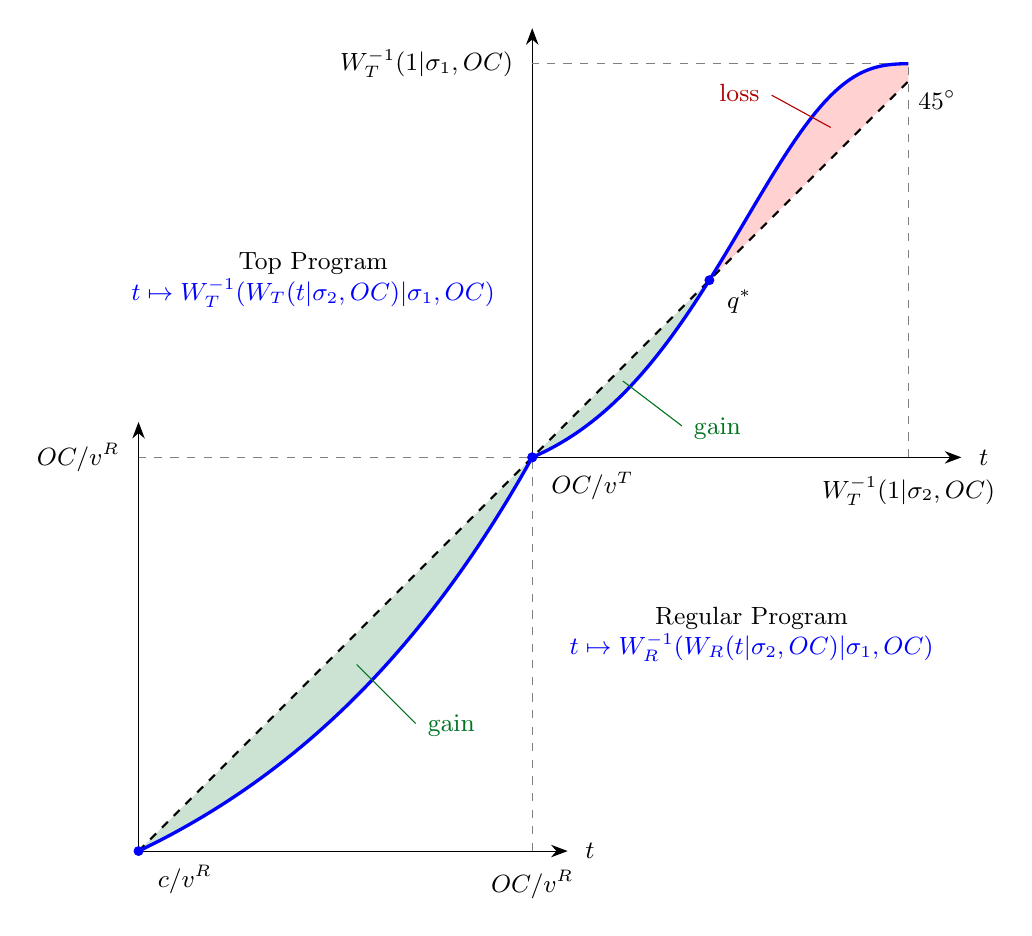
\begin{tikzpicture}[x=1cm,y=1cm]
  % the gains and the losses, beneath the 45 degree line
  \fill[darkgreen!20] plot coordinates {
(0.4000,0.4000) (0.4771,0.4372) (0.5534,0.4749) (0.6291,0.5130) (0.7041,0.5516)
(0.7784,0.5907) (0.8521,0.6302) (0.9252,0.6702) (0.9978,0.7108) (1.0698,0.7518)
(1.1413,0.7933) (1.2123,0.8353) (1.2828,0.8779) (1.3528,0.9210) (1.4224,0.9646)
(1.4915,1.0087) (1.5601,1.0534) (1.6284,1.0986) (1.6963,1.1444) (1.7637,1.1907)
(1.8308,1.2376) (1.8975,1.2851) (1.9639,1.3332) (2.0299,1.3818) (2.0955,1.4311)
(2.1608,1.4810) (2.2258,1.5314) (2.2905,1.5825) (2.3549,1.6342) (2.4189,1.6865)
(2.4827,1.7395) (2.5462,1.7931) (2.6094,1.8474) (2.6723,1.9024) (2.7350,1.9580)
(2.7974,2.0143) (2.8595,2.0713) (2.9214,2.1289) (2.9831,2.1873) (3.0445,2.2464)
(3.1056,2.3062) (3.1666,2.3668) (3.2273,2.4281) (3.2878,2.4901) (3.3480,2.5529)
(3.4081,2.6165) (3.4679,2.6808) (3.5276,2.7459) (3.5870,2.8118) (3.6463,2.8785)
(3.7053,2.9460) (3.7641,3.0143) (3.8228,3.0835) (3.8813,3.1535) (3.9396,3.2244)
(3.9977,3.2961) (4.0556,3.3687) (4.1134,3.4422) (4.1710,3.5165) (4.2284,3.5918)
(4.2857,3.6679) (4.3428,3.7450) (4.3998,3.8231) (4.4565,3.9020) (4.5132,3.9820)
(4.5696,4.0629) (4.6260,4.1447) (4.6822,4.2276) (4.7382,4.3114) (4.7941,4.3963)
(4.8498,4.4822) (4.9055,4.5691) (4.9609,4.6571) (5.0163,4.7461) (5.0715,4.8362)
(5.1265,4.9274) (5.1815,5.0197) (5.2363,5.1131) (5.2910,5.2076) (5.3456,5.3032)
(5.4000,5.4000) (5.4000,5.4000) (0.4000,0.4000)};
  \fill[darkgreen!20] plot coordinates {
(5.4000,5.4000) (5.4109,5.4047) (5.4218,5.4095) (5.4328,5.4144) (5.4437,5.4193)
(5.4547,5.4243) (5.4657,5.4293) (5.4767,5.4344) (5.4878,5.4395) (5.4988,5.4447)
(5.5099,5.4500) (5.5210,5.4553) (5.5321,5.4607) (5.5433,5.4661) (5.5544,5.4716)
(5.5656,5.4772) (5.5768,5.4828) (5.5880,5.4885) (5.5993,5.4942) (5.6105,5.5000)
(5.6218,5.5059) (5.6332,5.5119) (5.6445,5.5179) (5.6559,5.5240) (5.6673,5.5302)
(5.6787,5.5364) (5.6901,5.5427) (5.7016,5.5491) (5.7131,5.5555) (5.7246,5.5621)
(5.7362,5.5687) (5.7478,5.5753) (5.7594,5.5821) (5.7710,5.5889) (5.7827,5.5958)
(5.7944,5.6028) (5.8061,5.6099) (5.8178,5.6170) (5.8296,5.6243) (5.8414,5.6316)
(5.8533,5.6390) (5.8651,5.6465) (5.8770,5.6541) (5.8890,5.6617) (5.9009,5.6695)
(5.9129,5.6773) (5.9249,5.6853) (5.9370,5.6933) (5.9491,5.7014) (5.9612,5.7096)
(5.9734,5.7179) (5.9856,5.7264) (5.9978,5.7349) (6.0100,5.7435) (6.0223,5.7522)
(6.0347,5.7610) (6.0470,5.7699) (6.0594,5.7789) (6.0719,5.7880) (6.0843,5.7972)
(6.0968,5.8066) (6.1094,5.8160) (6.1220,5.8256) (6.1346,5.8352) (6.1472,5.8450)
(6.1599,5.8549) (6.1727,5.8649) (6.1854,5.8751) (6.1982,5.8853) (6.2111,5.8957)
(6.2240,5.9062) (6.2369,5.9168) (6.2499,5.9275) (6.2629,5.9384) (6.2759,5.9494)
(6.2890,5.9605) (6.3022,5.9717) (6.3153,5.9831) (6.3286,5.9946) (6.3418,6.0063)
(6.3551,6.0181) (6.3685,6.0300) (6.3819,6.0421) (6.3953,6.0543) (6.4088,6.0667)
(6.4223,6.0792) (6.4359,6.0918) (6.4495,6.1046) (6.4632,6.1176) (6.4769,6.1307)
(6.4907,6.1440) (6.5045,6.1574) (6.5184,6.1710) (6.5323,6.1847) (6.5462,6.1986)
(6.5602,6.2127) (6.5743,6.2269) (6.5884,6.2413) (6.6026,6.2559) (6.6168,6.2706)
(6.6311,6.2856) (6.6454,6.3007) (6.6598,6.3159) (6.6742,6.3314) (6.6887,6.3470)
(6.7032,6.3629) (6.7178,6.3789) (6.7325,6.3951) (6.7472,6.4115) (6.7620,6.4281)
(6.7768,6.4449) (6.7917,6.4619) (6.8067,6.4791) (6.8217,6.4965) (6.8368,6.5141)
(6.8519,6.5319) (6.8671,6.5499) (6.8823,6.5681) (6.8977,6.5866) (6.9131,6.6053)
(6.9285,6.6242) (6.9441,6.6433) (6.9596,6.6626) (6.9753,6.6822) (6.9910,6.7020)
(7.0068,6.7220) (7.0227,6.7423) (7.0386,6.7628) (7.0547,6.7836) (7.0707,6.8046)
(7.0869,6.8258) (7.1031,6.8473) (7.1195,6.8690) (7.1359,6.8910) (7.1523,6.9133)
(7.1689,6.9358) (7.1855,6.9586) (7.2022,6.9817) (7.2190,7.0050) (7.2359,7.0286)
(7.2529,7.0524) (7.2699,7.0766) (7.2870,7.1010) (7.3043,7.1257) (7.3216,7.1507)
(7.3390,7.1760) (7.3565,7.2015) (7.3741,7.2274) (7.3918,7.2536) (7.4096,7.2800)
(7.4274,7.3068) (7.4454,7.3338) (7.4635,7.3612) (7.4817,7.3889) (7.5000,7.4169)
(7.5184,7.4452) (7.5369,7.4738) (7.5555,7.5028) (7.5743,7.5320) (7.5931,7.5616)
(7.6121,7.5915) (7.6311,7.6218) (7.6469,7.6469) (5.4000,5.4000)};
  \fill[red!18] plot coordinates {
(7.6503,7.6524) (7.6697,7.6833) (7.6891,7.7145) (7.7087,7.7461) (7.7284,7.7780)
(7.7482,7.8103) (7.7682,7.8429) (7.7883,7.8758) (7.8086,7.9091) (7.8289,7.9427)
(7.8495,7.9767) (7.8702,8.0110) (7.8910,8.0457) (7.9120,8.0807) (7.9331,8.1160)
(7.9544,8.1517) (7.9759,8.1878) (7.9976,8.2242) (8.0194,8.2609) (8.0414,8.2980)
(8.0635,8.3354) (8.0859,8.3732) (8.1084,8.4113) (8.1312,8.4497) (8.1541,8.4884)
(8.1773,8.5275) (8.2007,8.5669) (8.2242,8.6066) (8.2480,8.6466) (8.2721,8.6869)
(8.2963,8.7275) (8.3208,8.7684) (8.3456,8.8096) (8.3706,8.8510) (8.3959,8.8927)
(8.4214,8.9347) (8.4473,8.9769) (8.4734,9.0192) (8.4998,9.0618) (8.5266,9.1046)
(8.5536,9.1476) (8.5810,9.1907) (8.6088,9.2339) (8.6369,9.2772) (8.6654,9.3206)
(8.6943,9.3641) (8.7236,9.4075) (8.7533,9.4510) (8.7835,9.4944) (8.8141,9.5377)
(8.8453,9.5809) (8.8769,9.6239) (8.9091,9.6668) (8.9419,9.7093) (8.9753,9.7515)
(9.0093,9.7933) (9.0440,9.8347) (9.0794,9.8755) (9.1156,9.9158) (9.1527,9.9553)
(9.1906,9.9941) (9.2295,10.0320) (9.2694,10.0689) (9.3105,10.1047) (9.3528,10.1392)
(9.3965,10.1724) (9.4417,10.2041) (9.4886,10.2341) (9.5375,10.2622) (9.5885,10.2883)
(9.6421,10.3122) (9.6988,10.3337) (9.7590,10.3525) (9.8238,10.3684) (9.8945,10.3812)
(9.9732,10.3907) (10.0642,10.3970) (10.1778,10.4000) (10.1778,10.1778) (7.6469,7.6469)};
  % the 45 degree line runs through both squares and stops where it
  % leaves the top square built by the two q = 1 quantiles
  \draw[black,dashed,thick] (0.40,0.40) -- (10.18,10.18);
  \node[anchor=north west,font=\small] at (10.18,10.18) {$45^{\circ}$};
  % --- regular program ---
  \draw[-{Stealth[length=6pt]},black] (0.40,0.40) -- (5.85,0.40);
  \draw[-{Stealth[length=6pt]},black] (0.40,0.40) -- (0.40,5.85);
  \node[anchor=west,font=\small] at (5.95,0.40) {$t$};
  \node[anchor=north west,font=\small] at (0.52,0.34) {$c/v^R$};
  \draw[gray,dashed] (5.40,0.40) -- (5.40,5.40) -- (0.40,5.40);
  \node[anchor=north,font=\small] at (5.40,0.28) {$OC/v^R$};
  \node[anchor=east,font=\small] at (0.28,5.40) {$OC/v^R$};
  \draw[blue,very thick] plot[smooth] coordinates {
(0.4000,0.4000) (0.4771,0.4372) (0.5534,0.4749) (0.6291,0.5130) (0.7041,0.5516)
(0.7784,0.5907) (0.8521,0.6302) (0.9252,0.6702) (0.9978,0.7108) (1.0698,0.7518)
(1.1413,0.7933) (1.2123,0.8353) (1.2828,0.8779) (1.3528,0.9210) (1.4224,0.9646)
(1.4915,1.0087) (1.5601,1.0534) (1.6284,1.0986) (1.6963,1.1444) (1.7637,1.1907)
(1.8308,1.2376) (1.8975,1.2851) (1.9639,1.3332) (2.0299,1.3818) (2.0955,1.4311)
(2.1608,1.4810) (2.2258,1.5314) (2.2905,1.5825) (2.3549,1.6342) (2.4189,1.6865)
(2.4827,1.7395) (2.5462,1.7931) (2.6094,1.8474) (2.6723,1.9024) (2.7350,1.9580)
(2.7974,2.0143) (2.8595,2.0713) (2.9214,2.1289) (2.9831,2.1873) (3.0445,2.2464)
(3.1056,2.3062) (3.1666,2.3668) (3.2273,2.4281) (3.2878,2.4901) (3.3480,2.5529)
(3.4081,2.6165) (3.4679,2.6808) (3.5276,2.7459) (3.5870,2.8118) (3.6463,2.8785)
(3.7053,2.9460) (3.7641,3.0143) (3.8228,3.0835) (3.8813,3.1535) (3.9396,3.2244)
(3.9977,3.2961) (4.0556,3.3687) (4.1134,3.4422) (4.1710,3.5165) (4.2284,3.5918)
(4.2857,3.6679) (4.3428,3.7450) (4.3998,3.8231) (4.4565,3.9020) (4.5132,3.9820)
(4.5696,4.0629) (4.6260,4.1447) (4.6822,4.2276) (4.7382,4.3114) (4.7941,4.3963)
(4.8498,4.4822) (4.9055,4.5691) (4.9609,4.6571) (5.0163,4.7461) (5.0715,4.8362)
(5.1265,4.9274) (5.1815,5.0197) (5.2363,5.1131) (5.2910,5.2076) (5.3456,5.3032)
(5.4000,5.4000)};
  \fill[blue] (0.40,0.40) circle (1.8pt) (5.40,5.40) circle (1.8pt);
  \draw[darkgreen,thin] (3.92,2.02) -- (3.17,2.77);
  \node[darkgreen,anchor=west,font=\small] at (3.95,1.99) {gain};
  % the title sits in the empty quadrant to the right of its square
  \node[anchor=west,font=\small,align=center] at (5.75,3.15) {Regular Program\\\textcolor{blue}{$t\mapsto W_R^{-1}(W_R(t|\sigma_2,OC)|\sigma_1,OC)$}};
  % --- top program ---
  \draw[-{Stealth[length=6pt]},black] (5.40,5.40) -- (10.85,5.40);
  \draw[-{Stealth[length=6pt]},black] (5.40,5.40) -- (5.40,10.85);
  \node[anchor=west,font=\small] at (10.95,5.40) {$t$};
  \node[anchor=north west,font=\small] at (5.52,5.34) {$OC/v^T$};
  \draw[gray,dashed] (10.18,5.40) -- (10.18,10.40) -- (5.40,10.40);
  \node[anchor=north,font=\small] at (10.18,5.28) {$W_T^{-1}(1|\sigma_2,OC)$};
  \node[anchor=east,font=\small] at (5.28,10.40) {$W_T^{-1}(1|\sigma_1,OC)$};
  \draw[blue,very thick] plot[smooth] coordinates {
(5.4000,5.4000) (5.4109,5.4047) (5.4218,5.4095) (5.4328,5.4144) (5.4437,5.4193)
(5.4547,5.4243) (5.4657,5.4293) (5.4767,5.4344) (5.4878,5.4395) (5.4988,5.4447)
(5.5099,5.4500) (5.5210,5.4553) (5.5321,5.4607) (5.5433,5.4661) (5.5544,5.4716)
(5.5656,5.4772) (5.5768,5.4828) (5.5880,5.4885) (5.5993,5.4942) (5.6105,5.5000)
(5.6218,5.5059) (5.6332,5.5119) (5.6445,5.5179) (5.6559,5.5240) (5.6673,5.5302)
(5.6787,5.5364) (5.6901,5.5427) (5.7016,5.5491) (5.7131,5.5555) (5.7246,5.5621)
(5.7362,5.5687) (5.7478,5.5753) (5.7594,5.5821) (5.7710,5.5889) (5.7827,5.5958)
(5.7944,5.6028) (5.8061,5.6099) (5.8178,5.6170) (5.8296,5.6243) (5.8414,5.6316)
(5.8533,5.6390) (5.8651,5.6465) (5.8770,5.6541) (5.8890,5.6617) (5.9009,5.6695)
(5.9129,5.6773) (5.9249,5.6853) (5.9370,5.6933) (5.9491,5.7014) (5.9612,5.7096)
(5.9734,5.7179) (5.9856,5.7264) (5.9978,5.7349) (6.0100,5.7435) (6.0223,5.7522)
(6.0347,5.7610) (6.0470,5.7699) (6.0594,5.7789) (6.0719,5.7880) (6.0843,5.7972)
(6.0968,5.8066) (6.1094,5.8160) (6.1220,5.8256) (6.1346,5.8352) (6.1472,5.8450)
(6.1599,5.8549) (6.1727,5.8649) (6.1854,5.8751) (6.1982,5.8853) (6.2111,5.8957)
(6.2240,5.9062) (6.2369,5.9168) (6.2499,5.9275) (6.2629,5.9384) (6.2759,5.9494)
(6.2890,5.9605) (6.3022,5.9717) (6.3153,5.9831) (6.3286,5.9946) (6.3418,6.0063)
(6.3551,6.0181) (6.3685,6.0300) (6.3819,6.0421) (6.3953,6.0543) (6.4088,6.0667)
(6.4223,6.0792) (6.4359,6.0918) (6.4495,6.1046) (6.4632,6.1176) (6.4769,6.1307)
(6.4907,6.1440) (6.5045,6.1574) (6.5184,6.1710) (6.5323,6.1847) (6.5462,6.1986)
(6.5602,6.2127) (6.5743,6.2269) (6.5884,6.2413) (6.6026,6.2559) (6.6168,6.2706)
(6.6311,6.2856) (6.6454,6.3007) (6.6598,6.3159) (6.6742,6.3314) (6.6887,6.3470)
(6.7032,6.3629) (6.7178,6.3789) (6.7325,6.3951) (6.7472,6.4115) (6.7620,6.4281)
(6.7768,6.4449) (6.7917,6.4619) (6.8067,6.4791) (6.8217,6.4965) (6.8368,6.5141)
(6.8519,6.5319) (6.8671,6.5499) (6.8823,6.5681) (6.8977,6.5866) (6.9131,6.6053)
(6.9285,6.6242) (6.9441,6.6433) (6.9596,6.6626) (6.9753,6.6822) (6.9910,6.7020)
(7.0068,6.7220) (7.0227,6.7423) (7.0386,6.7628) (7.0547,6.7836) (7.0707,6.8046)
(7.0869,6.8258) (7.1031,6.8473) (7.1195,6.8690) (7.1359,6.8910) (7.1523,6.9133)
(7.1689,6.9358) (7.1855,6.9586) (7.2022,6.9817) (7.2190,7.0050) (7.2359,7.0286)
(7.2529,7.0524) (7.2699,7.0766) (7.2870,7.1010) (7.3043,7.1257) (7.3216,7.1507)
(7.3390,7.1760) (7.3565,7.2015) (7.3741,7.2274) (7.3918,7.2536) (7.4096,7.2800)
(7.4274,7.3068) (7.4454,7.3338) (7.4635,7.3612) (7.4817,7.3889) (7.5000,7.4169)
(7.5184,7.4452) (7.5369,7.4738) (7.5555,7.5028) (7.5743,7.5320) (7.5931,7.5616)
(7.6121,7.5915) (7.6311,7.6218) (7.6503,7.6524) (7.6697,7.6833) (7.6891,7.7145)
(7.7087,7.7461) (7.7284,7.7780) (7.7482,7.8103) (7.7682,7.8429) (7.7883,7.8758)
(7.8086,7.9091) (7.8289,7.9427) (7.8495,7.9767) (7.8702,8.0110) (7.8910,8.0457)
(7.9120,8.0807) (7.9331,8.1160) (7.9544,8.1517) (7.9759,8.1878) (7.9976,8.2242)
(8.0194,8.2609) (8.0414,8.2980) (8.0635,8.3354) (8.0859,8.3732) (8.1084,8.4113)
(8.1312,8.4497) (8.1541,8.4884) (8.1773,8.5275) (8.2007,8.5669) (8.2242,8.6066)
(8.2480,8.6466) (8.2721,8.6869) (8.2963,8.7275) (8.3208,8.7684) (8.3456,8.8096)
(8.3706,8.8510) (8.3959,8.8927) (8.4214,8.9347) (8.4473,8.9769) (8.4734,9.0192)
(8.4998,9.0618) (8.5266,9.1046) (8.5536,9.1476) (8.5810,9.1907) (8.6088,9.2339)
(8.6369,9.2772) (8.6654,9.3206) (8.6943,9.3641) (8.7236,9.4075) (8.7533,9.4510)
(8.7835,9.4944) (8.8141,9.5377) (8.8453,9.5809) (8.8769,9.6239) (8.9091,9.6668)
(8.9419,9.7093) (8.9753,9.7515) (9.0093,9.7933) (9.0440,9.8347) (9.0794,9.8755)
(9.1156,9.9158) (9.1527,9.9553) (9.1906,9.9941) (9.2295,10.0320) (9.2694,10.0689)
(9.3105,10.1047) (9.3528,10.1392) (9.3965,10.1724) (9.4417,10.2041) (9.4886,10.2341)
(9.5375,10.2622) (9.5885,10.2883) (9.6421,10.3122) (9.6988,10.3337) (9.7590,10.3525)
(9.8238,10.3684) (9.8945,10.3812) (9.9732,10.3907) (10.0642,10.3970) (10.1778,10.4000)};
  \fill[blue] (5.40,5.40) circle (1.8pt) (7.65,7.65) circle (1.8pt);
  \node[anchor=north west,font=\small] at (7.75,7.65) {$q^{*}$};
  \draw[darkgreen,thin] (7.30,5.80) -- (6.55,6.37);
  \node[darkgreen,anchor=west,font=\small] at (7.33,5.77) {gain};
  \draw[red!70!black,thin] (8.44,10.00) -- (9.19,9.59);
  \node[red!70!black,anchor=east,font=\small] at (8.41,10.03) {loss};
  % the title sits in the empty quadrant to the left of its square
  \node[anchor=east,font=\small,align=center] at (5.05,7.65) {Top Program\\\textcolor{blue}{$t\mapsto W_T^{-1}(W_T(t|\sigma_2,OC)|\sigma_1,OC)$}};
\end{tikzpicture}
% Caption kept here, deliberately not typeset - the figure carries a
% number only.  To restore it, move the line below into \caption{}.
% Both QQ plots carry the same $45^{\circ}$ reference line, so the two squares sit on a single diagonal. Below left, the regular program: the curve is anchored to the diagonal at both ends, since the marginal regular applicant wins with probability $c/v^R$ and the marginal top applicant with probability $OC/v^R$ whatever the noise, and it lies strictly below (above) in between, so under a convex (concave) mills ratio every regular applicant gains (loses). Above right, the top program: the curve crosses the diagonal at the pivotal rank $q^*$. Convex: $v^R=0.4$, $c=0.03$.
\caption{Convex Mills Ratio}
\label{fig:qq_diag_convex}
\end{figure}


\subsubsection{What about the application ratio?}\label{section:fixedoc_application_ratio}: Holding fixed the marginal top applicant's opportunity cost, mills ratio curvature also governs the response of the application ratio $a^T/a^R$ following a rise in noise. Higher noise lowers the marginal top applicant $\hat{\theta}^T_{\sigma_2,OC} < \hat{\theta}^T_{\sigma_1,OC}$ so the number of top applicants rises. 

\noindent The effect of an increase in noise on the number of applicants in the regular program is generally ambiguous. To resolve this, recall the two opposite forces discussed in Section \ref{section:competing_forces}. Under a convex mills ratio, the regular acceptance rate rises because regular applicants who remain see a rise in their winning probability that offsets the lower quality applicant pool. This requires the inflow of low-merit applicants at the extensive margin to be sufficiently small relative to the outflow of the best regular applicants to the top program. Thus, any rise in regular applicants is small enough such that the ratio $a^T/a^R$ rises after an increase in noise. This is stated in the following proposition: 

\begin{proposition}\label{prop:noiseincrease_ratioapps}
Suppose that $g$ is log-concave with strictly decreasing mills ratio. Fix $\sigma_1<\sigma_2$ and an opportunity cost $OC$ such that $(OC,\sigma)\in\mathcal{D}$ for all $\sigma\in[\sigma_1,\sigma_2]$. If the mills ratio is convex (concave), then the share of top applicants $a^T/(a^T+a^R)$ weakly increases (decreases) following an increase in noise, when we hold fixed the opportunity cost of the marginal top applicant.
% \begin{align*}
%   \dfrac{1 - G(\hat{\theta}^T_{\sigma_1,OC})}{G(\hat{\theta}^T_{\sigma_1,OC}) - G(\hat{\theta}^R_{\sigma_1,OC})} \substack{\leq \\ (\geq)} \dfrac{1 - G(\hat{\theta}^T_{\sigma_2,OC})}{G(\hat{\theta}^T_{\sigma_2,OC}) - G(\hat{\theta}^R_{\sigma_2,OC})}
% \end{align*}
\end{proposition}

\subsection{Proving the headline result}

% Section 4.3.1 - R(OC,sigma) shifted up by higher noise, convex mills ratio.
% GENERATED BY generate_figures.py - edit that file, not this one.
% sigma_1=0.9: OC_1=0.2758 (dR/dOC=+0.9064), stable (regular True, top True); no crossing from above
% sigma_2=2.25: OC_2=0.2448 (dR/dOC=+1.5439), Definition 3 conditions (regular True, top True)
\begin{figure}[htbp]
\centering
\pgfplotsset{ocshift/.style={
  width=12.0cm, height=8.4cm,
  xmin=0.13, xmax=0.33, ymin=0.381, ymax=0.673,
  axis x line=bottom, axis y line=left,
  axis line style={-{Stealth[length=6pt]},black}, clip=false,
  xlabel={$OC$}, ylabel={$\mathcal{R}(OC,\sigma)$},
  every axis x label/.style={at={(current axis.south east)},anchor=west,xshift=9pt},
  every axis y label/.style={at={(current axis.north west)},anchor=south,yshift=7pt},
  tick label style={font=\footnotesize}, label style={font=\footnotesize},
  title style={font=\footnotesize, yshift=2pt},
  tick style={black},
  xtick={0.1400,0.2448,0.2758}, xticklabels={,,},
  ytick={0.5700}, yticklabels={$\lambda^{R}$},
  tick label style={font=\small}, label style={font=\small},
}}

\begin{tikzpicture}
\begin{axis}[ocshift]
  \addplot[black,dashed,thick,samples=2,domain=0.13:0.33] {0.5700};
  \draw[gray,dashed] (axis cs:0.24476,0.381) -- (axis cs:0.24476,0.57000);
  \draw[gray,dashed] (axis cs:0.27580,0.381) -- (axis cs:0.27580,0.61688);
  \node[anchor=north,font=\small] at (axis cs:0.14000,0.3788) {$c$};
  \node[anchor=north,font=\small] at (axis cs:0.24476,0.3788) {$OC_2$};
  \node[anchor=north,font=\small] at (axis cs:0.27580,0.3788) {$OC_1$};
  \addplot[blue,very thick,smooth] coordinates {
(0.1442,0.4060) (0.1468,0.4097) (0.1495,0.4134) (0.1521,0.4171) (0.1547,0.4209)
(0.1574,0.4246) (0.1600,0.4283) (0.1627,0.4320) (0.1654,0.4357) (0.1681,0.4395)
(0.1708,0.4432) (0.1734,0.4469) (0.1761,0.4505) (0.1788,0.4542) (0.1815,0.4578)
(0.1842,0.4615) (0.1869,0.4651) (0.1895,0.4687) (0.1922,0.4722) (0.1948,0.4758)
(0.1975,0.4793) (0.2001,0.4828) (0.2027,0.4862) (0.2054,0.4896) (0.2080,0.4930)
(0.2105,0.4963) (0.2131,0.4996) (0.2157,0.5028) (0.2182,0.5060) (0.2207,0.5092)
(0.2232,0.5123) (0.2257,0.5154) (0.2281,0.5184) (0.2305,0.5213) (0.2329,0.5242)
(0.2353,0.5271) (0.2377,0.5298) (0.2400,0.5326) (0.2423,0.5352) (0.2446,0.5378)
(0.2468,0.5404) (0.2491,0.5429) (0.2512,0.5453) (0.2534,0.5476) (0.2555,0.5499)
(0.2576,0.5522) (0.2597,0.5543) (0.2617,0.5564) (0.2638,0.5585) (0.2657,0.5605)
(0.2677,0.5624) (0.2696,0.5642) (0.2715,0.5660) (0.2733,0.5677) (0.2752,0.5694)
(0.2770,0.5710) (0.2787,0.5726) (0.2804,0.5741) (0.2821,0.5756) (0.2838,0.5770)
(0.2854,0.5783) (0.2870,0.5797) (0.2886,0.5809) (0.2901,0.5822) (0.2916,0.5834)
(0.2931,0.5845) (0.2946,0.5857) (0.2960,0.5868) (0.2974,0.5878) (0.2987,0.5889)};
  \addplot[blue,very thick,dash pattern=on 6pt off 3pt,smooth] coordinates {
(0.1442,0.4062) (0.1468,0.4102) (0.1495,0.4143) (0.1521,0.4185) (0.1547,0.4228)
(0.1574,0.4271) (0.1600,0.4315) (0.1627,0.4360) (0.1654,0.4404) (0.1681,0.4449)
(0.1708,0.4495) (0.1734,0.4540) (0.1761,0.4585) (0.1788,0.4630) (0.1815,0.4675)
(0.1842,0.4720) (0.1869,0.4765) (0.1895,0.4810) (0.1922,0.4854) (0.1948,0.4899)
(0.1975,0.4942) (0.2001,0.4986) (0.2027,0.5029) (0.2054,0.5072) (0.2080,0.5115)
(0.2105,0.5157) (0.2131,0.5199) (0.2157,0.5240) (0.2182,0.5281) (0.2207,0.5321)
(0.2232,0.5361) (0.2257,0.5400) (0.2281,0.5439) (0.2305,0.5478) (0.2329,0.5516)
(0.2353,0.5553) (0.2377,0.5590) (0.2400,0.5626) (0.2423,0.5662) (0.2446,0.5697)
(0.2468,0.5732) (0.2491,0.5766) (0.2512,0.5799) (0.2534,0.5832) (0.2555,0.5865)
(0.2576,0.5897) (0.2597,0.5928) (0.2617,0.5959) (0.2638,0.5989) (0.2657,0.6019)
(0.2677,0.6048) (0.2696,0.6076) (0.2715,0.6104) (0.2733,0.6132) (0.2752,0.6159)
(0.2770,0.6186) (0.2787,0.6212) (0.2804,0.6238) (0.2821,0.6264) (0.2838,0.6289)
(0.2854,0.6314) (0.2870,0.6339) (0.2886,0.6363) (0.2901,0.6388) (0.2916,0.6412)
(0.2931,0.6436) (0.2946,0.6460) (0.2960,0.6484) (0.2974,0.6508) (0.2987,0.6532)};
  % the dots carry a white rim so they stand out against the curves
  \filldraw[fill=darkgreen,draw=white,line width=0.8pt] (axis cs:0.27580,0.57000) circle (3.2pt);
  % the new stable crossing
  \filldraw[fill=red,draw=white,line width=0.8pt] (axis cs:0.24476,0.57000) circle (3.2pt);
  % where the guide at OC_1 meets the new curve
  \filldraw[fill=orange,draw=white,line width=0.8pt] (axis cs:0.27580,0.61688) circle (3.2pt);
  \node[blue,anchor=west,font=\small] at (axis cs:0.3019,0.6532) {$\mathcal{R}(OC,\sigma_2)$};
  \node[blue,anchor=west,font=\small] at (axis cs:0.3019,0.5889) {$\mathcal{R}(OC,\sigma_1)$};
\end{axis}
\end{tikzpicture}
\caption{}
% Caption kept here, deliberately not typeset - the figure carries a
% number only.  To restore it, move the line below into \caption{}.
% The regular acceptance rate curve before (solid) and after (dashed) a rise in noise from $\sigma_1$ to $\sigma_2$. The mills ratio is convex, so the curve shifts upwards. It crosses $\lambda^R$ from below at $OC_1$, a stable equilibrium in the sense of Definition \ref{def:equilibrium}; after the shift, the crossing from below moves to the lower opportunity cost $OC_2$, which is also stable. $\sigma_1=0.9$, $\sigma_2=2.25$; $F$ standard logistic, $\sigma=0.9$; $G=\mathrm{Beta}(2,2)$ on $[-2.5,2.5]$; $\lambda^T=0.3$, $v^R/v^T=0.35$, $\lambda^R=0.57$, $c/v^R=0.4$.
\label{fig:oc_noise_shift}
\end{figure}


\subsubsection{The effect of noise on opportunity costs}: We can now prove Proposition \ref{prop:mainresult}. We first show that a marginal rise in noise yields convergence to a new (stable) equilibrium with lower opportunity costs when the mills ratio is convex, and higher opportunity costs when the mills ratio is concave:

\begin{proposition}\label{prop:noise_oc}
Suppose that $g$ is log-concave with strictly decreasing mills ratio, and we are initially at an interior stable equilibrium. If the mills ratio is convex (concave), then a marginal rise in evaluation noise implies the existence of a new interior stable equilibrium in which the opportunity cost of the marginal top applicant is weakly lower (higher) than before. 
\end{proposition}

\noindent To see this, suppose we are initially at a stable fixed payline equilibrium $(\hat{\theta}^R_1, \hat{\theta}^T_1)$, with corresponding opportunity cost $OC_1$ and initial noise $\sigma_1$. By Proposition \ref{prop:reg_acceptance_stable_frombelow}, the regular acceptance rate curve $OC\mapsto \mathcal{R}(OC,\sigma_1)$ crosses $\lambda^R$ from below at $OC_1$. Figure \ref{fig:oc_noise_shift} plots the regular acceptance rate curve (the solid blue line) whose intersection with the horizontal line $\lambda^R$ at the green dot represents the original equilibrium. 

\noindent Suppose that the mills ratio is convex. By Proposition \ref{prop:reg_noise}, an increase in noise from $\sigma_1$ to $\sigma_2$ holding fixed a given opportunity cost necessarily involves an increase in the regular program average acceptance rate. Graphically, this is depicted as an upwards shift in the regular acceptance rate curve from the solid blue curve to the dashed one. At the original opportunity cost $OC_1$, a rise in noise raises the regular acceptance rate above the target payline $\lambda^R$ (see the orange dot). Thus, to restore the target payline, the regular score cutoff must rise. This leads to a fall in the average acceptance rate and in the opportunity cost of the marginal top applicant. The result is a new stable equilibrium at the red dot, with a new opportunity cost $OC_2$ that is smaller than before\footnote{If for instance the initial equilibrium was unstable, it may be the case that the curve $OC\mapsto \mathcal{R}(OC,\sigma_1)$ initially crossed the horizontal line $\lambda^R$ from above. An increase in noise then shifts this curve upwards, but the new intersection of the curve with the horizontal $\lambda^R$ curve occurs at a \textit{higher} opportunity cost than before.}. 

% Section 4.3.1 - best responses at the initial equilibrium OC_1 of Figure oc_noise_shift.
% GENERATED BY generate_figures.py - edit that file, not this one.
% Blue : xhat^R     |-> thetahat^T_top(xhat^R|sigma)   from 3.1.6, DECREASING.
% Red  : thetahat^T |-> xhat^R_reg(thetahat^T|sigma)   from 3.1.7, INCREASING.
% One falls and one rises, so they meet exactly once.
% Green: trajectories of the Proposition 4 partial-adjustment ODE.
% Its Jacobian has trace -(kappa_R+kappa_T) < 0 and determinant
% kappa_R kappa_T (1 - B_T' B_R'), so local asymptotic stability is
% exactly B_T' B_R' < 1; here B_T' B_R' = -2.6565, so the det
% factor is 3.6565 > 0.
% Equilibrium: xhat^R*=1.0065, thetahat^T*=2.1882 (implied thetahat^R*=0.6416).
\pgfplotsset{geaxis/.style={
  width=15.5cm, height=9.4cm,
  xmin=0.76, xmax=1.30, ymin=2.020, ymax=2.330,
  axis x line=bottom, axis y line=left,
  axis line style={-{Stealth[length=6pt]},black}, clip=false,
  xlabel={$\hat{x}^R$}, ylabel={$\hat{\theta}^T$},
  every axis x label/.style={at={(current axis.south east)},anchor=west,xshift=9pt},
  every axis y label/.style={at={(current axis.north west)},anchor=south,yshift=7pt},
  tick label style={font=\footnotesize}, label style={font=\footnotesize},
  title style={font=\footnotesize, yshift=2pt},
  tick style={black},
  xtick={1.0065}, xticklabels={$\hat{x}^R_1$},
  ytick={2.1882}, yticklabels={$\hat{\theta}^T_1$},
}}

\begin{figure}[htbp]
\centering
\begin{tikzpicture}
\begin{axis}[geaxis, legend cell align=left,
  legend entries={{$\hat{x}^R\mapsto\hat{\theta}^T_{top}(\hat{x}^R|\sigma_1)$},{$\hat{x}^R\mapsto\hat{\theta}^T_{top}(\hat{x}^R|\sigma_2)$},{$\hat{\theta}^T\mapsto\hat{x}^R_{reg}(\hat{\theta}^T|\lambda^R,\sigma_1)$},{$\hat{\theta}^T\mapsto\hat{x}^R_{reg}(\hat{\theta}^T|\mathcal{R}(OC_1,\sigma_2),\sigma_2)$},{$\hat{\theta}^T\mapsto\hat{x}^R_{reg}(\hat{\theta}^T|\lambda^R,\sigma_2)$}},
  legend style={at={(0.99,0.02)}, anchor=south east, font=\footnotesize,
    draw=gray!40, fill=white, row sep=1pt}]
  \addlegendimage{blue,very thick}
  \addlegendimage{blue,very thick,dash pattern=on 6pt off 3pt}
  \addlegendimage{red,very thick}
  \addlegendimage{red,very thick,dash pattern=on 6pt off 3pt}
  \addlegendimage{red,very thick,dash pattern=on 2pt off 2pt}
  \draw[gray,dashed] (axis cs:1.00649,2.020) -- (axis cs:1.00649,2.18817);
  \draw[gray,dashed] (axis cs:0.76,2.18817) -- (axis cs:1.00649,2.18817);
  \addplot[darkgreen!45,very thick,samples=2,domain=0.8383:1.1483] {x + 1.18168};
  \node[darkgreen,anchor=west,font=\footnotesize,inner sep=3pt] at (axis cs:1.1483,2.3300) {$OC_1,\sigma_1$};
  \addplot[darkgreen!45,very thick,samples=2,domain=0.7600:1.0302] {x + 1.29985};
  \node[darkgreen,anchor=south,font=\footnotesize,inner sep=3pt] at (axis cs:1.0302,2.3300) {$OC_1,\sigma_2$};
  \addplot[blue,very thick,smooth] coordinates {
(0.9693,2.3289) (0.9699,2.3271) (0.9706,2.3252) (0.9712,2.3233) (0.9719,2.3214)
(0.9725,2.3195) (0.9732,2.3176) (0.9738,2.3157) (0.9744,2.3137) (0.9751,2.3117)
(0.9757,2.3097) (0.9764,2.3078) (0.9770,2.3057) (0.9776,2.3037) (0.9783,2.3017)
(0.9789,2.2996) (0.9796,2.2975) (0.9802,2.2954) (0.9808,2.2933) (0.9815,2.2912)
(0.9821,2.2890) (0.9828,2.2869) (0.9834,2.2847) (0.9841,2.2825) (0.9847,2.2802)
(0.9853,2.2780) (0.9860,2.2757) (0.9866,2.2734) (0.9873,2.2711) (0.9879,2.2688)
(0.9885,2.2664) (0.9892,2.2640) (0.9898,2.2616) (0.9905,2.2592) (0.9911,2.2568)
(0.9918,2.2543) (0.9924,2.2518) (0.9930,2.2492) (0.9937,2.2467) (0.9943,2.2441)
(0.9950,2.2415) (0.9956,2.2388) (0.9962,2.2361) (0.9969,2.2334) (0.9975,2.2307)
(0.9982,2.2279) (0.9988,2.2251) (0.9995,2.2222) (1.0001,2.2194) (1.0007,2.2164)
(1.0014,2.2135) (1.0020,2.2105) (1.0027,2.2074) (1.0033,2.2043) (1.0039,2.2012)
(1.0046,2.1980) (1.0052,2.1947) (1.0059,2.1914) (1.0065,2.1881) (1.0072,2.1847)
(1.0078,2.1812) (1.0084,2.1777) (1.0091,2.1741) (1.0097,2.1705) (1.0104,2.1667)
(1.0110,2.1629) (1.0116,2.1590) (1.0123,2.1551) (1.0129,2.1510) (1.0136,2.1469)
(1.0142,2.1426) (1.0148,2.1383) (1.0155,2.1338) (1.0161,2.1292) (1.0168,2.1245)
(1.0174,2.1197) (1.0181,2.1146) (1.0187,2.1095) (1.0193,2.1041) (1.0200,2.0986)
(1.0206,2.0928) (1.0213,2.0867) (1.0219,2.0804) (1.0225,2.0738) (1.0232,2.0668)
(1.0238,2.0594) (1.0245,2.0515) (1.0251,2.0430) (1.0258,2.0337) (1.0264,2.0233)};
  \addplot[red,very thick,smooth] coordinates {
(0.9105,2.0229) (0.9147,2.0293) (0.9188,2.0357) (0.9228,2.0421) (0.9269,2.0485)
(0.9309,2.0549) (0.9348,2.0613) (0.9388,2.0678) (0.9427,2.0742) (0.9466,2.0806)
(0.9504,2.0870) (0.9543,2.0934) (0.9580,2.0998) (0.9618,2.1062) (0.9655,2.1126)
(0.9692,2.1190) (0.9728,2.1254) (0.9764,2.1318) (0.9800,2.1382) (0.9835,2.1446)
(0.9870,2.1510) (0.9905,2.1574) (0.9939,2.1638) (0.9973,2.1702) (1.0006,2.1766)
(1.0039,2.1830) (1.0071,2.1894) (1.0103,2.1958) (1.0135,2.2022) (1.0166,2.2087)
(1.0197,2.2151) (1.0227,2.2215) (1.0257,2.2279) (1.0286,2.2343) (1.0314,2.2407)
(1.0343,2.2471) (1.0370,2.2535) (1.0398,2.2599) (1.0424,2.2663) (1.0450,2.2727)
(1.0476,2.2791) (1.0501,2.2855) (1.0525,2.2919) (1.0549,2.2983) (1.0573,2.3047)
(1.0595,2.3111) (1.0617,2.3175) (1.0639,2.3239)};
  % the best responses at the higher noise, whose payline is the
  % regular acceptance rate at the original opportunity cost
  \addplot[blue,very thick,dash pattern=on 6pt off 3pt,smooth] coordinates {
(0.8102,2.3290) (0.8110,2.3268) (0.8119,2.3245) (0.8127,2.3223) (0.8135,2.3200)
(0.8143,2.3177) (0.8151,2.3154) (0.8159,2.3131) (0.8168,2.3107) (0.8176,2.3083)
(0.8184,2.3060) (0.8192,2.3036) (0.8200,2.3011) (0.8209,2.2987) (0.8217,2.2962)
(0.8225,2.2937) (0.8233,2.2912) (0.8241,2.2887) (0.8249,2.2861) (0.8258,2.2836)
(0.8266,2.2810) (0.8274,2.2783) (0.8282,2.2757) (0.8290,2.2730) (0.8298,2.2703)
(0.8307,2.2676) (0.8315,2.2648) (0.8323,2.2621) (0.8331,2.2593) (0.8339,2.2564)
(0.8348,2.2536) (0.8356,2.2507) (0.8364,2.2477) (0.8372,2.2448) (0.8380,2.2418)
(0.8388,2.2387) (0.8397,2.2357) (0.8405,2.2326) (0.8413,2.2294) (0.8421,2.2263)
(0.8429,2.2230) (0.8437,2.2198) (0.8446,2.2165) (0.8454,2.2132) (0.8462,2.2098)
(0.8470,2.2063) (0.8478,2.2029) (0.8487,2.1993) (0.8495,2.1958) (0.8503,2.1921)
(0.8511,2.1884) (0.8519,2.1847) (0.8527,2.1809) (0.8536,2.1770) (0.8544,2.1731)
(0.8552,2.1691) (0.8560,2.1651) (0.8568,2.1609) (0.8576,2.1567) (0.8585,2.1524)
(0.8593,2.1480) (0.8601,2.1436) (0.8609,2.1390) (0.8617,2.1344) (0.8626,2.1296)
(0.8634,2.1247) (0.8642,2.1197) (0.8650,2.1146) (0.8658,2.1094) (0.8666,2.1040)
(0.8675,2.0985) (0.8683,2.0927) (0.8691,2.0869) (0.8699,2.0808) (0.8707,2.0745)
(0.8715,2.0680) (0.8724,2.0612) (0.8732,2.0541) (0.8740,2.0467) (0.8748,2.0389)
(0.8756,2.0307) (0.8764,2.0221)};
  \addplot[red,very thick,dash pattern=on 6pt off 3pt,smooth] coordinates {
(0.7821,2.0229) (0.7860,2.0293) (0.7899,2.0357) (0.7938,2.0421) (0.7976,2.0485)
(0.8014,2.0549) (0.8051,2.0613) (0.8089,2.0678) (0.8126,2.0742) (0.8162,2.0806)
(0.8199,2.0870) (0.8235,2.0934) (0.8270,2.0998) (0.8306,2.1062) (0.8341,2.1126)
(0.8375,2.1190) (0.8410,2.1254) (0.8444,2.1318) (0.8477,2.1382) (0.8510,2.1446)
(0.8543,2.1510) (0.8575,2.1574) (0.8607,2.1638) (0.8639,2.1702) (0.8670,2.1766)
(0.8701,2.1830) (0.8731,2.1894) (0.8761,2.1958) (0.8791,2.2022) (0.8820,2.2087)
(0.8848,2.2151) (0.8877,2.2215) (0.8904,2.2279) (0.8932,2.2343) (0.8958,2.2407)
(0.8985,2.2471) (0.9010,2.2535) (0.9036,2.2599) (0.9060,2.2663) (0.9085,2.2727)
(0.9108,2.2791) (0.9132,2.2855) (0.9154,2.2919) (0.9176,2.2983) (0.9198,2.3047)
(0.9219,2.3111) (0.9239,2.3175) (0.9259,2.3239)};
  % back at the original regular payline, still at the higher noise
  \addplot[red,very thick,dash pattern=on 2pt off 2pt,smooth] coordinates {
(0.7986,2.0229) (0.8025,2.0293) (0.8064,2.0357) (0.8103,2.0421) (0.8141,2.0485)
(0.8180,2.0549) (0.8217,2.0613) (0.8255,2.0678) (0.8292,2.0742) (0.8329,2.0806)
(0.8366,2.0870) (0.8402,2.0934) (0.8438,2.0998) (0.8473,2.1062) (0.8509,2.1126)
(0.8543,2.1190) (0.8578,2.1254) (0.8612,2.1318) (0.8646,2.1382) (0.8679,2.1446)
(0.8712,2.1510) (0.8745,2.1574) (0.8777,2.1638) (0.8809,2.1702) (0.8840,2.1766)
(0.8871,2.1830) (0.8902,2.1894) (0.8932,2.1958) (0.8962,2.2022) (0.8991,2.2087)
(0.9020,2.2151) (0.9048,2.2215) (0.9076,2.2279) (0.9104,2.2343) (0.9131,2.2407)
(0.9157,2.2471) (0.9183,2.2535) (0.9208,2.2599) (0.9233,2.2663) (0.9258,2.2727)
(0.9282,2.2791) (0.9305,2.2855) (0.9328,2.2919) (0.9350,2.2983) (0.9372,2.3047)
(0.9393,2.3111) (0.9414,2.3175) (0.9434,2.3239)};
  \filldraw[fill=darkgreen,draw=white,line width=0.8pt] (axis cs:1.00649,2.18817) circle (3.2pt);
  \draw[gray,dashed] (axis cs:0.86194,2.0200) -- (axis cs:0.86194,2.13318) -- (axis cs:0.7600,2.13318);
  \draw[black] (axis cs:0.86194,2.0200) -- ++(0pt,-3pt);
  \draw[black] (axis cs:0.7600,2.13318) -- ++(-3pt,0pt);
  \node[anchor=north west,font=\footnotesize,inner sep=2pt,yshift=-3pt] at (axis cs:0.86194,2.0200) {$\hat{x}^R_2$};
  \node[anchor=east,font=\footnotesize,inner sep=2pt,xshift=-3pt] at (axis cs:0.7600,2.13318) {$\hat{\theta}^T_2$};
  \draw[gray,dashed] (axis cs:0.85752,2.0200) -- (axis cs:0.85752,2.15737) -- (axis cs:0.7600,2.15737);
  \draw[black] (axis cs:0.85752,2.0200) -- ++(0pt,-3pt);
  \draw[gray,dashed] (axis cs:0.85752,2.0200) -- ++(0pt,-16pt);
  \draw[black] (axis cs:0.7600,2.15737) -- ++(-3pt,0pt);
  \node[anchor=north,font=\footnotesize,inner sep=2pt,yshift=-16pt] at (axis cs:0.85752,2.0200) {$\hat{x}^{R}_{\sigma_2,OC_1}$};
  \node[anchor=east,font=\footnotesize,inner sep=2pt,xshift=-3pt] at (axis cs:0.7600,2.15737) {$\hat{\theta}^{T}_{\sigma_2,OC_1}$};
  \filldraw[fill=orange,draw=white,line width=0.8pt] (axis cs:0.85752,2.15737) circle (3.2pt);
  \filldraw[fill=red,draw=white,line width=0.8pt] (axis cs:0.86194,2.13318) circle (3.2pt);
\end{axis}
\end{tikzpicture}
\caption{}
% Caption kept here, deliberately not typeset - the figure carries a
% number only.  To restore it, move the line below into \caption{}.
% Best responses at the initial equilibrium $OC_1$ of Figure \ref{fig:oc_noise_shift}, with the lines along which the marginal top applicant faces opportunity cost $OC_1$ at $\sigma_1=0.9$ and at $\sigma_2=0.99$ (a smaller rise than in Figure \ref{fig:oc_noise_shift}). $F$ standard logistic, $\sigma=0.9$; $G=\mathrm{Beta}(2,2)$ on $[-2.5,2.5]$; $\lambda^T=0.3$, $v^R/v^T=0.35$, $\lambda^R=0.57$, $c/v^R=0.4$.
\label{fig:br_shift}
\end{figure}


% % Section 4.3.1 - best responses at the initial equilibrium OC_1 of Figure oc_noise_shift.
% GENERATED BY generate_figures.py - edit that file, not this one.
% Blue : xhat^R     |-> thetahat^T_top(xhat^R|sigma)   from 3.1.6, DECREASING.
% Red  : thetahat^T |-> xhat^R_reg(thetahat^T|sigma)   from 3.1.7, INCREASING.
% One falls and one rises, so they meet exactly once.
% Green: trajectories of the Proposition 4 partial-adjustment ODE.
% Its Jacobian has trace -(kappa_R+kappa_T) < 0 and determinant
% kappa_R kappa_T (1 - B_T' B_R'), so local asymptotic stability is
% exactly B_T' B_R' < 1; here B_T' B_R' = -2.6565, so the det
% factor is 3.6565 > 0.
% Equilibrium: xhat^R*=1.0065, thetahat^T*=2.1882 (implied thetahat^R*=0.6416).
\pgfplotsset{geaxis/.style={
  width=15.5cm, height=9.4cm,
  xmin=0.76, xmax=1.30, ymin=2.020, ymax=2.330,
  axis x line=bottom, axis y line=left,
  axis line style={-{Stealth[length=6pt]},black}, clip=false,
  xlabel={$\hat{x}^R$}, ylabel={$\hat{\theta}^T$},
  every axis x label/.style={at={(current axis.south east)},anchor=west,xshift=9pt},
  every axis y label/.style={at={(current axis.north west)},anchor=south,yshift=7pt},
  tick label style={font=\footnotesize}, label style={font=\footnotesize},
  title style={font=\footnotesize, yshift=2pt},
  tick style={black},
  xtick={1.0065}, xticklabels={$\hat{x}^R_1$},
  ytick={2.1882}, yticklabels={$\hat{\theta}^T_1$},
}}

\begin{figure}[htbp]
\centering
\begin{tikzpicture}
\begin{axis}[geaxis, legend cell align=left,
  legend entries={{$\hat{x}^R\mapsto\hat{\theta}^T_{top}(\hat{x}^R|\sigma_1)$},{$\hat{x}^R\mapsto\hat{\theta}^T_{top}(\hat{x}^R|\sigma_2)$},{$\hat{\theta}^T\mapsto\hat{x}^R_{reg}(\hat{\theta}^T|\lambda^R,\sigma_1)$},{$\hat{\theta}^T\mapsto\hat{x}^R_{reg}(\hat{\theta}^T|\mathcal{R}(OC_1,\sigma_2),\sigma_2)$},{$\hat{\theta}^T\mapsto\hat{x}^R_{reg}(\hat{\theta}^T|\lambda^R,\sigma_2)$}},
  legend style={at={(0.99,0.02)}, anchor=south east, font=\footnotesize,
    draw=gray!40, fill=white, row sep=1pt}]
  \addlegendimage{blue,very thick,opacity=0.4}
  \addlegendimage{blue,very thick,dash pattern=on 6pt off 3pt,opacity=0.4}
  \addlegendimage{red,very thick,opacity=0.4}
  \addlegendimage{red,very thick,dash pattern=on 6pt off 3pt,opacity=0.4}
  \addlegendimage{red,very thick,dash pattern=on 2pt off 2pt,opacity=0.4}
  \draw[gray,dashed] (axis cs:1.00649,2.020) -- (axis cs:1.00649,2.18817);
  \draw[gray,dashed] (axis cs:0.76,2.18817) -- (axis cs:1.00649,2.18817);
  \addplot[darkgreen!45,very thick,opacity=0.4,samples=2,domain=0.8383:1.1483] {x + 1.18168};
  \node[darkgreen,anchor=west,font=\footnotesize,inner sep=3pt] at (axis cs:1.1483,2.3300) {$OC_1,\sigma_1$};
  \addplot[darkgreen!45,very thick,opacity=0.4,samples=2,domain=0.7600:1.0302] {x + 1.29985};
  \node[darkgreen,anchor=south,font=\footnotesize,inner sep=3pt] at (axis cs:1.0302,2.3300) {$OC_1,\sigma_2$};
  \addplot[blue,very thick,opacity=0.4,smooth] coordinates {
(0.9693,2.3289) (0.9699,2.3271) (0.9706,2.3252) (0.9712,2.3233) (0.9719,2.3214)
(0.9725,2.3195) (0.9732,2.3176) (0.9738,2.3157) (0.9744,2.3137) (0.9751,2.3117)
(0.9757,2.3097) (0.9764,2.3078) (0.9770,2.3057) (0.9776,2.3037) (0.9783,2.3017)
(0.9789,2.2996) (0.9796,2.2975) (0.9802,2.2954) (0.9808,2.2933) (0.9815,2.2912)
(0.9821,2.2890) (0.9828,2.2869) (0.9834,2.2847) (0.9841,2.2825) (0.9847,2.2802)
(0.9853,2.2780) (0.9860,2.2757) (0.9866,2.2734) (0.9873,2.2711) (0.9879,2.2688)
(0.9885,2.2664) (0.9892,2.2640) (0.9898,2.2616) (0.9905,2.2592) (0.9911,2.2568)
(0.9918,2.2543) (0.9924,2.2518) (0.9930,2.2492) (0.9937,2.2467) (0.9943,2.2441)
(0.9950,2.2415) (0.9956,2.2388) (0.9962,2.2361) (0.9969,2.2334) (0.9975,2.2307)
(0.9982,2.2279) (0.9988,2.2251) (0.9995,2.2222) (1.0001,2.2194) (1.0007,2.2164)
(1.0014,2.2135) (1.0020,2.2105) (1.0027,2.2074) (1.0033,2.2043) (1.0039,2.2012)
(1.0046,2.1980) (1.0052,2.1947) (1.0059,2.1914) (1.0065,2.1881) (1.0072,2.1847)
(1.0078,2.1812) (1.0084,2.1777) (1.0091,2.1741) (1.0097,2.1705) (1.0104,2.1667)
(1.0110,2.1629) (1.0116,2.1590) (1.0123,2.1551) (1.0129,2.1510) (1.0136,2.1469)
(1.0142,2.1426) (1.0148,2.1383) (1.0155,2.1338) (1.0161,2.1292) (1.0168,2.1245)
(1.0174,2.1197) (1.0181,2.1146) (1.0187,2.1095) (1.0193,2.1041) (1.0200,2.0986)
(1.0206,2.0928) (1.0213,2.0867) (1.0219,2.0804) (1.0225,2.0738) (1.0232,2.0668)
(1.0238,2.0594) (1.0245,2.0515) (1.0251,2.0430) (1.0258,2.0337) (1.0264,2.0233)};
  \addplot[red,very thick,opacity=0.4,smooth] coordinates {
(0.9105,2.0229) (0.9147,2.0293) (0.9188,2.0357) (0.9228,2.0421) (0.9269,2.0485)
(0.9309,2.0549) (0.9348,2.0613) (0.9388,2.0678) (0.9427,2.0742) (0.9466,2.0806)
(0.9504,2.0870) (0.9543,2.0934) (0.9580,2.0998) (0.9618,2.1062) (0.9655,2.1126)
(0.9692,2.1190) (0.9728,2.1254) (0.9764,2.1318) (0.9800,2.1382) (0.9835,2.1446)
(0.9870,2.1510) (0.9905,2.1574) (0.9939,2.1638) (0.9973,2.1702) (1.0006,2.1766)
(1.0039,2.1830) (1.0071,2.1894) (1.0103,2.1958) (1.0135,2.2022) (1.0166,2.2087)
(1.0197,2.2151) (1.0227,2.2215) (1.0257,2.2279) (1.0286,2.2343) (1.0314,2.2407)
(1.0343,2.2471) (1.0370,2.2535) (1.0398,2.2599) (1.0424,2.2663) (1.0450,2.2727)
(1.0476,2.2791) (1.0501,2.2855) (1.0525,2.2919) (1.0549,2.2983) (1.0573,2.3047)
(1.0595,2.3111) (1.0617,2.3175) (1.0639,2.3239)};
  % the best responses at the higher noise, whose payline is the
  % regular acceptance rate at the original opportunity cost
  \addplot[blue,very thick,dash pattern=on 6pt off 3pt,opacity=0.4,smooth] coordinates {
(0.8102,2.3290) (0.8110,2.3268) (0.8119,2.3245) (0.8127,2.3223) (0.8135,2.3200)
(0.8143,2.3177) (0.8151,2.3154) (0.8159,2.3131) (0.8168,2.3107) (0.8176,2.3083)
(0.8184,2.3060) (0.8192,2.3036) (0.8200,2.3011) (0.8209,2.2987) (0.8217,2.2962)
(0.8225,2.2937) (0.8233,2.2912) (0.8241,2.2887) (0.8249,2.2861) (0.8258,2.2836)
(0.8266,2.2810) (0.8274,2.2783) (0.8282,2.2757) (0.8290,2.2730) (0.8298,2.2703)
(0.8307,2.2676) (0.8315,2.2648) (0.8323,2.2621) (0.8331,2.2593) (0.8339,2.2564)
(0.8348,2.2536) (0.8356,2.2507) (0.8364,2.2477) (0.8372,2.2448) (0.8380,2.2418)
(0.8388,2.2387) (0.8397,2.2357) (0.8405,2.2326) (0.8413,2.2294) (0.8421,2.2263)
(0.8429,2.2230) (0.8437,2.2198) (0.8446,2.2165) (0.8454,2.2132) (0.8462,2.2098)
(0.8470,2.2063) (0.8478,2.2029) (0.8487,2.1993) (0.8495,2.1958) (0.8503,2.1921)
(0.8511,2.1884) (0.8519,2.1847) (0.8527,2.1809) (0.8536,2.1770) (0.8544,2.1731)
(0.8552,2.1691) (0.8560,2.1651) (0.8568,2.1609) (0.8576,2.1567) (0.8585,2.1524)
(0.8593,2.1480) (0.8601,2.1436) (0.8609,2.1390) (0.8617,2.1344) (0.8626,2.1296)
(0.8634,2.1247) (0.8642,2.1197) (0.8650,2.1146) (0.8658,2.1094) (0.8666,2.1040)
(0.8675,2.0985) (0.8683,2.0927) (0.8691,2.0869) (0.8699,2.0808) (0.8707,2.0745)
(0.8715,2.0680) (0.8724,2.0612) (0.8732,2.0541) (0.8740,2.0467) (0.8748,2.0389)
(0.8756,2.0307) (0.8764,2.0221)};
  \addplot[red,very thick,dash pattern=on 6pt off 3pt,opacity=0.4,smooth] coordinates {
(0.7821,2.0229) (0.7860,2.0293) (0.7899,2.0357) (0.7938,2.0421) (0.7976,2.0485)
(0.8014,2.0549) (0.8051,2.0613) (0.8089,2.0678) (0.8126,2.0742) (0.8162,2.0806)
(0.8199,2.0870) (0.8235,2.0934) (0.8270,2.0998) (0.8306,2.1062) (0.8341,2.1126)
(0.8375,2.1190) (0.8410,2.1254) (0.8444,2.1318) (0.8477,2.1382) (0.8510,2.1446)
(0.8543,2.1510) (0.8575,2.1574) (0.8607,2.1638) (0.8639,2.1702) (0.8670,2.1766)
(0.8701,2.1830) (0.8731,2.1894) (0.8761,2.1958) (0.8791,2.2022) (0.8820,2.2087)
(0.8848,2.2151) (0.8877,2.2215) (0.8904,2.2279) (0.8932,2.2343) (0.8958,2.2407)
(0.8985,2.2471) (0.9010,2.2535) (0.9036,2.2599) (0.9060,2.2663) (0.9085,2.2727)
(0.9108,2.2791) (0.9132,2.2855) (0.9154,2.2919) (0.9176,2.2983) (0.9198,2.3047)
(0.9219,2.3111) (0.9239,2.3175) (0.9259,2.3239)};
  % back at the original regular payline, still at the higher noise
  \addplot[red,very thick,dash pattern=on 2pt off 2pt,opacity=0.4,smooth] coordinates {
(0.7986,2.0229) (0.8025,2.0293) (0.8064,2.0357) (0.8103,2.0421) (0.8141,2.0485)
(0.8180,2.0549) (0.8217,2.0613) (0.8255,2.0678) (0.8292,2.0742) (0.8329,2.0806)
(0.8366,2.0870) (0.8402,2.0934) (0.8438,2.0998) (0.8473,2.1062) (0.8509,2.1126)
(0.8543,2.1190) (0.8578,2.1254) (0.8612,2.1318) (0.8646,2.1382) (0.8679,2.1446)
(0.8712,2.1510) (0.8745,2.1574) (0.8777,2.1638) (0.8809,2.1702) (0.8840,2.1766)
(0.8871,2.1830) (0.8902,2.1894) (0.8932,2.1958) (0.8962,2.2022) (0.8991,2.2087)
(0.9020,2.2151) (0.9048,2.2215) (0.9076,2.2279) (0.9104,2.2343) (0.9131,2.2407)
(0.9157,2.2471) (0.9183,2.2535) (0.9208,2.2599) (0.9233,2.2663) (0.9258,2.2727)
(0.9282,2.2791) (0.9305,2.2855) (0.9328,2.2919) (0.9350,2.2983) (0.9372,2.3047)
(0.9393,2.3111) (0.9414,2.3175) (0.9434,2.3239)};
  \draw[black,thick,-{Stealth[length=6pt]},shorten <=5pt,shorten >=5pt] (axis cs:1.00649,2.18817) -- (axis cs:0.85752,2.15737);
  \draw[black,thick,-{Stealth[length=6pt]},shorten <=5pt,shorten >=5pt] (axis cs:0.85752,2.15737) -- (axis cs:0.86194,2.13318);
  \filldraw[fill=darkgreen,draw=white,line width=0.8pt] (axis cs:1.00649,2.18817) circle (3.2pt);
  \draw[gray,dashed] (axis cs:0.86194,2.0200) -- (axis cs:0.86194,2.13318) -- (axis cs:0.7600,2.13318);
  \draw[black] (axis cs:0.86194,2.0200) -- ++(0pt,-3pt);
  \draw[black] (axis cs:0.7600,2.13318) -- ++(-3pt,0pt);
  \node[anchor=north west,font=\footnotesize,inner sep=2pt,yshift=-3pt] at (axis cs:0.86194,2.0200) {$\hat{x}^R_2$};
  \node[anchor=east,font=\footnotesize,inner sep=2pt,xshift=-3pt] at (axis cs:0.7600,2.13318) {$\hat{\theta}^T_2$};
  \draw[gray,dashed] (axis cs:0.85752,2.0200) -- (axis cs:0.85752,2.15737) -- (axis cs:0.7600,2.15737);
  \draw[black] (axis cs:0.85752,2.0200) -- ++(0pt,-3pt);
  \draw[gray,dashed] (axis cs:0.85752,2.0200) -- ++(0pt,-16pt);
  \draw[black] (axis cs:0.7600,2.15737) -- ++(-3pt,0pt);
  \node[anchor=north,font=\footnotesize,inner sep=2pt,yshift=-16pt] at (axis cs:0.85752,2.0200) {$\hat{x}^{R}_{\sigma_2,OC_1}$};
  \node[anchor=east,font=\footnotesize,inner sep=2pt,xshift=-3pt] at (axis cs:0.7600,2.15737) {$\hat{\theta}^{T}_{\sigma_2,OC_1}$};
  \filldraw[fill=orange,draw=white,line width=0.8pt] (axis cs:0.85752,2.15737) circle (3.2pt);
  \filldraw[fill=red,draw=white,line width=0.8pt] (axis cs:0.86194,2.13318) circle (3.2pt);
\end{axis}
\end{tikzpicture}
\caption{}
% Caption kept here, deliberately not typeset - the figure carries a
% number only.  To restore it, move the line below into \caption{}.
% Best responses at the initial equilibrium $OC_1$ of Figure \ref{fig:oc_noise_shift}, with the lines along which the marginal top applicant faces opportunity cost $OC_1$ at $\sigma_1=0.9$ and at $\sigma_2=0.99$ (a smaller rise than in Figure \ref{fig:oc_noise_shift}). $F$ standard logistic, $\sigma=0.9$; $G=\mathrm{Beta}(2,2)$ on $[-2.5,2.5]$; $\lambda^T=0.3$, $v^R/v^T=0.35$, $\lambda^R=0.57$, $c/v^R=0.4$.
\label{fig:br_shift_arrows}
\end{figure}


\noindent This can also be understood using the best response curves that characterize a stable fixed payline equilibrium. The intersection of the solid red and blue curves in Figure \ref{fig:br_shift} at the green dot refers to the original stable equilibrium. The green curve labeled $OC_1,\sigma_1$ is a level curve that represents all combinations of $\hat{x}^R$ and $\hat{\theta}^T$ that keep the opportunity cost fixed at its initial level:
\begin{align*}
    v^R\bar{F}\left(\dfrac{\hat{x}^R - \hat{\theta}^T}{\sigma_1}\right) = OC_1
\end{align*}
A rise in noise shifts the level curve representing all combinations of points that keep the opportunity cost fixed at $OC_1$. Suppose that the regular program score cutoff is less than the marginal top applicant $\hat{x}_1^R < \hat{\theta}_1^T$ at the initial equilibrium\footnote{This is without loss of generality. If instead we have $\hat{x}_1^R \geq \hat{\theta}_1^T$, then the new level curve after the rise in noise will lie weakly below the curve labeled $OC_1,\sigma_1$. The rest of the argument in this section continues analogously with no change in its final conclusion.}. Since the level curve has slope 1, all points on this curve are such that $\hat{x}^R < \hat{\theta}^T$. The rise in noise reduces the regular probability of acceptance for any fixed marginal top applicant, thereby decreasing his opportunity cost below $OC_1$. To keep the opportunity cost fixed at $OC_1$, the regular score cutoff must fall. This yields a new green level curve labeled $OC_1,\sigma_2$ that lies above the original level curve.

\noindent We now ask where the best response curves shift following an increase in noise from $\sigma_1$ to $\sigma_2$, but where we allow the regular program average acceptance rate to adjust so as to keep the opportunity cost fixed at its initial level $OC_1$. First, the intersection of these two new best response curves must lie on the new green line $OC_1,\sigma_2$ to keep the opportunity cost fixed. Moreover, this intersection must lie below $\hat{\theta}_1^T$ because higher noise yields a lower-merit marginal top applicant (see Proposition \ref{prop:topmarginal_cost_noise}). This yields the dashed red/blue best response curves intersecting at the orange dot (which also coincides with the orange dot in Figure \ref{fig:oc_noise_shift}). Thus, to keep the opportunity cost fixed following a rise in noise, the regular score cutoff falls from $\hat{x}^R_1$ to $\hat{x}^R_{\sigma_2,OC_1}$ and the marginal top applicant falls from $\hat{\theta}_1^T$ to $\hat{\theta}_{\sigma_2,OC_1}^T$. 

\noindent The blue dashed line is the best response curve in the top program following a rise in noise. The red dashed line $\hat{\theta}^T\mapsto \hat{x}^R_{reg}(\hat{\theta}^T|\mathcal{R}(OC_1,\sigma_2),\sigma_2)$ is the best response curve after the rise in noise to $\sigma_2$ and a change in the payline from $\lambda^R$ to $\mathcal{R}(OC_1,\sigma_2)$. Under a convex mills ratio, the current regular acceptance rate lies above the target payline $\mathcal{R}(OC_1,\sigma_2)>\lambda^R$. Thus, since a fall in the regular acceptance rate can only be facilitated by a rise in the regular score cutoff, the best response curve $\hat{\theta}^T\mapsto \hat{x}^R_{reg}(\hat{\theta}^T|\lambda^R,\sigma_2)$ would lie below the best response curve $\hat{\theta}^T\mapsto \hat{x}^R_{reg}(\hat{\theta}^T|\mathcal{R}(OC_1,\sigma_2),\sigma_2)$. It then follows that the red point is the new stable fixed payline equilibrium following the noise increase. Importantly, this point lies below the green level curve labeled $OC_1,\sigma_2$, indicating that the opportunity cost $OC_2$ at this new equilibrium is smaller than $OC_1$. 

\noindent If instead, the mills ratio were concave, then the current regular acceptance rate at the orange dot in Figure \ref{fig:br_shift} would be lower than the target payline $\mathcal{R}(OC_1,\sigma_2)<\lambda^R$. It therefore follows that the best response curve $\hat{\theta}^T\mapsto \hat{x}^R_{reg}(\hat{\theta}^T|\lambda^R,\sigma_2)$ would lie \textit{above} the best response curve $\hat{\theta}^T\mapsto \hat{x}^R_{reg}(\hat{\theta}^T|\mathcal{R}(OC_1,\sigma_2),\sigma_2)$. The new stable fixed payline equilibrium would lie above the green level curve labeled $OC_1,\sigma_2$, indicating that the opportunity cost at this new equilibrium is \textit{larger} than $OC_1$. 


\subsubsection{The effect of noise on the application ratio $a^T/a^R$}: We now claim that the mills ratio convexity also implies a rise in the application ratio after an increase in noise:

\begin{proposition}\label{prop:noise_ratio}
Suppose that $g$ is log-concave with strictly decreasing mills ratio, and we are initially at an interior stable equilibrium. If the mills ratio is convex (concave), a marginal rise in evaluation noise implies the existence of a new interior stable equilibrium in which the application ratio $a^T/a^R$ is weakly larger (lower) than before.
\end{proposition}

\noindent To see why, start again at the green dot of Figure \ref{fig:br_shift} and raise noise from $\sigma_1$ to $\sigma_2$, holding the opportunity cost fixed at $OC_1$. The move to the orange dot lowers the marginal top applicant and, by Proposition \ref{prop:noiseincrease_ratioapps}, raises the top to regular ratio of applicants $a^T/a^R$. At the orange dot, the regular acceptance rate (weakly) exceeds the regular payline $\lambda^R$. The rise in the regular score cutoff to restore this payline deters the lowest merit regular applicants and pushes the best regular applicants to apply to the top program instead. Consequently, $a^T$ rises and $a^R$ falls. It thus follows that the new stable equilibrium after the noise increase has a higher application ratio than before. 

\section{Multiple Fields: Equilibria and stability}

\noindent We now turn to the problem of vertical choice with multiple fields. We may focus on 2 scientific fields without loss of generality\footnote{All our results naturally extend to the case of more than 2 fields.}. To emphasize the role of evaluation noise, let us assume for convenience that both fields are identical\footnote{That is, let us assume that both fields have an identical distribution of applicant merit $G$, the same screening technology $f$, identical application costs $c$, and each researcher earns the same benefit $v^P$ from applying to program $P\in \{R,T\}$.} except for the fact that field 2 has higher evaluation noise than field 1 $\sigma_2>\sigma_1$. For a given program $P\in\{R,T\}$, let $B^P$ denote the total budget of grants and suppose that this budget is distributed across scientific fields according to the following proportional allocation rule:
\begin{align*}
    B_i^P = \dfrac{a_i^P}{a_1^P+a_2^P}B^P
\end{align*}
That is, the budget of grants allocated to field $i$ is proportional to the number of applicants $a_i^P$ from that field. Proportional allocation can be equivalently understood as a budget rule that equalizes the average acceptance rate across different fields, while fully exhausting each program's budget:
\begin{align*}
    \dfrac{B_1^P}{a_1^P} = \dfrac{B_2^P}{a_2^P} \quad B_1^P + B_2^P = B^P
\end{align*}
We are particularly interested in an equilibrium that arises from the following iterative process:
\vspace{-5pt}
\begin{enumerate}[label=(\arabic*),ref=\thelemma(\arabic*)]
  \item The central administrator first commits to paylines $\lambda = (\lambda^R,\lambda^T)$ for each program. 
  \item Given these paylines, this yields a stable fixed payline equilibrium in each field as described in Definition \ref{def:equilibrium}. Let  $\hat{\theta}_i^P(\lambda), \hat{x}^P_i(\lambda)$ be the corresponding equilibrium marginal applicants and score cutoffs. The corresponding total number of grants awarded in the regular program is:
  \begin{align*}
      A^R = \sum_{i=1,2}\int_{\hat{\theta}_i^R(\lambda)}^{\hat{\theta}_i^T(\lambda)}\bar{F}_{\sigma_i}(\hat{x}^R_i(\lambda)|\theta) \,dG(\theta)
   \end{align*}
   Similarly, the corresponding number of grants awarded in the top program is:
   \begin{align*}
      A^T = \sum_{i=1,2}\int_{\hat{\theta}_i^T(\lambda)}^{\bar{\theta}}\bar{F}_{\sigma_i}(\hat{x}^T_i(\lambda)|\theta) \,dG(\theta)
   \end{align*}
   \item If $A^P > B^P$, the demand for grants exceeds the supply for program $P$ and thus the current payline is too lenient. The administrator then reduces the payline and we go back to step (2). Conversely, if $A^P < B^P$, the administrator instead raises the payline in program $P$. 
\end{enumerate} 
This process repeats until the total demand for grants equals the budget for both the top and regular program. This motivates the following definition of a stable equilibrium under proportional budget allocation:

\begin{definition}\label{def:multifieldequilibrium}
A stable proportional allocation equilibrium is a tuple of target paylines $\lambda^* = (\lambda^{R,*}, \lambda^{T,*})$ and field-specific marginal types $(\hat{\theta}^{R,*}_i, \hat{\theta}^{T,*}_i),i=1,2$ such that, for each program $P\in \{R,T\}$:
\vspace{-5pt}
\begin{enumerate}[label=(\arabic*),ref=\thedefinition(\arabic*)]
   \item For each field $i$, the equilibrium marginal types $(\hat{\theta}^{R,*}_i,\hat{\theta}^{T,*}_i )$ constitute a stable fixed payline equilibrium in the sense of Definition \ref{def:equilibrium} given target paylines $\lambda^{R,*},\lambda^{T,*}$.  
   \item The total demand for grants in both programs equals the supply $B^P$. 
\end{enumerate}
\end{definition}

\noindent Indeed, Proposition \ref{prop:multifield_stability} in the appendix shows that this definition of a stable proportional allocation equilibrium is sufficient to guarantee local stability under the aforementioned iterative process. 

\section{Do fields sort in equilibrium?}\label{section:multifield}

\subsubsection{The Multifield Headline Result}: In a (stable) proportional allocation equilibrium, will the higher-noise field sort into the more desirable top program or the less desirable regular program? We have the following result:

\begin{customprop}{1}
Suppose that $g$ is log-concave with strictly decreasing mills ratio. Consider some stable proportional allocation equilibrium. Under some technical regularity conditions\footnote{Formally, let $\lambda^{R,*}$ denote the common equilibrium regular program payline faced by both fields, and let $OC_i^*$ be the equilibrium opportunity cost of the marginal top applicant in field $i$. We assume that there exists a continuous map $OC^*:[\sigma_1,\sigma_2]\rightarrow (0,\infty)$ such that, for each $\sigma\in[\sigma_1,\sigma_2]$, we have that $(OC^*(\sigma),\sigma)\in \mathcal{D}$, $\mathcal{R}(OC^*(\sigma),\sigma) = \lambda^{R,*}$, and $OC^*(\sigma_i) = OC_i^*$ for $i=1,2$, where $\mathcal{D}$ is defined with top payline $\lambda^{T,*}$. We also assume that $(OC_1^*,\sigma)\in\mathcal{D}$ for all $\sigma\in[\sigma_1,\sigma_2]$, so that both marginal applicants remain interior when noise rises from $\sigma_1$ to $\sigma_2$ at field 1's opportunity cost.}, if the mills ratio of the merit distribution is convex (concave), we have that:
\vspace{-5pt}
\begin{enumerate}[label=(\arabic*),ref=\theinnercustomprop(\arabic*)]
   \item The opportunity cost of the marginal top applicant is weakly lower (higher) in the field with larger noise. 
   \item The percent of total applicants who apply to the top rather than regular program $a^T/(a^T+a^R)$ will be weakly larger (smaller) in the field with higher noise. 
   \item The ratio of grants awarded in the top to regular program $B_i^T/B_i^R$ will be weakly larger (smaller) in the field with higher noise. 
\end{enumerate}
\end{customprop}

\noindent That is, convexity of the mills ratio guarantees that the higher-noise field sorts into the top program, while the lower-noise field sorts into the regular program. As we will see, this outcome is a straightforward implication of the results we obtained in the single field environment. 

\noindent First, fix some stable proportional allocation equilibrium consisting of target paylines $\lambda^{R,*},\lambda^{T,*}$ and field-specific marginal types in both programs $(\hat{\theta}^{R,*}_i,\hat{\theta}^{T,*}_i)$. By definition, for each field $i$, the marginal types $(\hat{\theta}^{R,*}_i,\hat{\theta}^{T,*}_i)$ are stable fixed payline equilibria given target paylines $\lambda^{R,*},\lambda^{T,*}$. Now, plot the regular acceptance rate curves for both fields $OC\mapsto \mathcal{R}(OC,\sigma_i), i=1,2$. As discussed in Proposition \ref{prop:reg_acceptance_stable_frombelow}, for each field $i$, the opportunity cost $OC_i^*$ at which the field's regular acceptance rate curve intersects the horizontal line $\lambda^{R,*}$ exactly coincides with the equilibrium opportunity cost in that field. Moreover, we know from Proposition \ref{prop:reg_acceptance_stable_frombelow} that, in both fields, the regular acceptance rate curve $OC\mapsto \mathcal{R}(OC,\sigma_i)$ crosses the horizontal line from below because the equilibria in both fields were assumed to be stable. 

\noindent A natural next step is to determine whether the regular acceptance rate curve in the high-noise field lies above or below the corresponding curve in the low-noise field. Suppose that the mills ratio of the common merit distribution is convex. As discussed in Proposition \ref{prop:reg_noise}, the regular acceptance rate curve in the high-noise field $OC\mapsto \mathcal{R}(OC,\sigma_2)$ must lie above the corresponding curve in the low-noise field $OC\mapsto \mathcal{R}(OC,\sigma_1)$. This is depicted in Figure \ref{fig:field_convex}. It follows that (under the maintained regularity conditions) the equilibrium opportunity cost in field 1 is larger than that in field 2 $OC_1^*\geq OC_2^*$. Conversely, under a concave mills ratio, the regular acceptance rate curve in the high-noise field $OC\mapsto \mathcal{R}(OC,\sigma_2)$ must lie \textit{below} the corresponding curve in the low-noise field $OC\mapsto \mathcal{R}(OC,\sigma_1)$, as depicted in Figure \ref{fig:field_concave}. It then follows that the equilibrium opportunity cost in the high-noise field is \textit{larger} than in the low-noise field. 

% Section 6.0.1 - regular acceptance curves of two fields, convex and concave.
% GENERATED BY generate_figures.py - edit that file, not this one.
% convex: sigma_1=0.9: OC_1*=0.2758; sigma_2=2.25: OC_2*=0.2448; both stable (Definition 3).
% concave: sigma_1=0.3: OC_1*=0.2382; sigma_2=0.6: OC_2*=0.2609; both stable (Definition 3).
\begin{figure}[htbp]
\centering
\begin{subfigure}[t]{0.49\textwidth}\centering
\pgfplotsset{fieldRa/.style={
  width=7.6cm, height=6.6cm,
  xmin=0.13, xmax=0.31, ymin=0.381, ymax=0.673,
  axis x line=bottom, axis y line=left,
  axis line style={-{Stealth[length=6pt]},black}, clip=false,
  xlabel={$OC$}, ylabel={$\mathcal{R}(OC,\sigma)$},
  every axis x label/.style={at={(current axis.south east)},anchor=west,xshift=9pt},
  every axis y label/.style={at={(current axis.north west)},anchor=south,yshift=7pt},
  tick label style={font=\footnotesize}, label style={font=\footnotesize},
  title style={font=\footnotesize, yshift=2pt},
  tick style={black},
  xtick={0.1400,0.2758,0.2448}, xticklabels={,,},
  ytick={0.5700}, yticklabels={$\lambda^{R,*}$},
  tick label style={font=\footnotesize}, label style={font=\footnotesize},
  title={(a) Convex mills ratio}, title style={font=\small, yshift=20pt},
}}

\begin{tikzpicture}[baseline=(current axis.south west)]
\begin{axis}[fieldRa]
  \addplot[black,dashed,thick,samples=2,domain=0.13:0.31] {0.5700};
  \draw[gray,dashed] (axis cs:0.27580,0.381) -- (axis cs:0.27580,0.61688);
  \draw[gray,dashed] (axis cs:0.24476,0.381) -- (axis cs:0.24476,0.57000);
  \node[anchor=north,font=\footnotesize] at (axis cs:0.14000,0.3788) {$c$};
  \node[anchor=north,font=\footnotesize] at (axis cs:0.24476,0.3788) {$OC_2^{*}$};
  \node[anchor=north,font=\footnotesize] at (axis cs:0.27580,0.3788) {$OC_1^{*}$};
  % the low noise field in blue, the high noise field in red
  \addplot[blue,very thick,smooth] coordinates {
(0.1442,0.4060) (0.1468,0.4097) (0.1495,0.4134) (0.1521,0.4171) (0.1547,0.4209)
(0.1574,0.4246) (0.1600,0.4283) (0.1627,0.4320) (0.1654,0.4357) (0.1681,0.4395)
(0.1708,0.4432) (0.1734,0.4469) (0.1761,0.4505) (0.1788,0.4542) (0.1815,0.4578)
(0.1842,0.4615) (0.1869,0.4651) (0.1895,0.4687) (0.1922,0.4722) (0.1948,0.4758)
(0.1975,0.4793) (0.2001,0.4828) (0.2027,0.4862) (0.2054,0.4896) (0.2080,0.4930)
(0.2105,0.4963) (0.2131,0.4996) (0.2157,0.5028) (0.2182,0.5060) (0.2207,0.5092)
(0.2232,0.5123) (0.2257,0.5154) (0.2281,0.5184) (0.2305,0.5213) (0.2329,0.5242)
(0.2353,0.5271) (0.2377,0.5298) (0.2400,0.5326) (0.2423,0.5352) (0.2446,0.5378)
(0.2468,0.5404) (0.2491,0.5429) (0.2512,0.5453) (0.2534,0.5476) (0.2555,0.5499)
(0.2576,0.5522) (0.2597,0.5543) (0.2617,0.5564) (0.2638,0.5585) (0.2657,0.5605)
(0.2677,0.5624) (0.2696,0.5642) (0.2715,0.5660) (0.2733,0.5677) (0.2752,0.5694)
(0.2770,0.5710) (0.2787,0.5726) (0.2804,0.5741) (0.2821,0.5756) (0.2838,0.5770)
(0.2854,0.5783) (0.2870,0.5797) (0.2886,0.5809) (0.2901,0.5822) (0.2916,0.5834)
(0.2931,0.5845) (0.2946,0.5857) (0.2960,0.5868) (0.2974,0.5878) (0.2987,0.5889)};
  \addplot[red,very thick,smooth] coordinates {
(0.1442,0.4062) (0.1468,0.4102) (0.1495,0.4143) (0.1521,0.4185) (0.1547,0.4228)
(0.1574,0.4271) (0.1600,0.4315) (0.1627,0.4360) (0.1654,0.4404) (0.1681,0.4449)
(0.1708,0.4495) (0.1734,0.4540) (0.1761,0.4585) (0.1788,0.4630) (0.1815,0.4675)
(0.1842,0.4720) (0.1869,0.4765) (0.1895,0.4810) (0.1922,0.4854) (0.1948,0.4899)
(0.1975,0.4942) (0.2001,0.4986) (0.2027,0.5029) (0.2054,0.5072) (0.2080,0.5115)
(0.2105,0.5157) (0.2131,0.5199) (0.2157,0.5240) (0.2182,0.5281) (0.2207,0.5321)
(0.2232,0.5361) (0.2257,0.5400) (0.2281,0.5439) (0.2305,0.5478) (0.2329,0.5516)
(0.2353,0.5553) (0.2377,0.5590) (0.2400,0.5626) (0.2423,0.5662) (0.2446,0.5697)
(0.2468,0.5732) (0.2491,0.5766) (0.2512,0.5799) (0.2534,0.5832) (0.2555,0.5865)
(0.2576,0.5897) (0.2597,0.5928) (0.2617,0.5959) (0.2638,0.5989) (0.2657,0.6019)
(0.2677,0.6048) (0.2696,0.6076) (0.2715,0.6104) (0.2733,0.6132) (0.2752,0.6159)
(0.2770,0.6186) (0.2787,0.6212) (0.2804,0.6238) (0.2821,0.6264) (0.2838,0.6289)
(0.2854,0.6314) (0.2870,0.6339) (0.2886,0.6363) (0.2901,0.6388) (0.2916,0.6412)
(0.2931,0.6436) (0.2946,0.6460) (0.2960,0.6484) (0.2974,0.6508) (0.2987,0.6532)};
  % each field's equilibrium, with a white rim so it stands out
  \filldraw[fill=blue,draw=white,line width=0.8pt] (axis cs:0.27580,0.57000) circle (3.2pt);
  \filldraw[fill=red,draw=white,line width=0.8pt] (axis cs:0.24476,0.57000) circle (3.2pt);
  % the high noise field's acceptance rate at OC_1^*
  \filldraw[fill=orange,draw=white,line width=0.8pt] (axis cs:0.27580,0.61688) circle (3.2pt);
\end{axis}
\end{tikzpicture}
\phantomsubcaption
\label{fig:field_convex}
\end{subfigure}
\hfill
\begin{subfigure}[t]{0.49\textwidth}\centering
\pgfplotsset{fieldRb/.style={
  width=7.6cm, height=6.6cm,
  xmin=0.11, xmax=0.31, ymin=0.373, ymax=0.759,
  axis x line=bottom, axis y line=left,
  axis line style={-{Stealth[length=6pt]},black}, clip=false,
  xlabel={$OC$}, ylabel={$\mathcal{R}(OC,\sigma)$},
  every axis x label/.style={at={(current axis.south east)},anchor=west,xshift=9pt},
  every axis y label/.style={at={(current axis.north west)},anchor=south,yshift=7pt},
  tick label style={font=\footnotesize}, label style={font=\footnotesize},
  title style={font=\footnotesize, yshift=2pt},
  tick style={black},
  xtick={0.1200,0.2382,0.2609}, xticklabels={,,},
  ytick={0.5830}, yticklabels={$\lambda^{R,*}$},
  tick label style={font=\footnotesize}, label style={font=\footnotesize},
  title={(b) Concave mills ratio}, title style={font=\small, yshift=20pt},
}}

\begin{tikzpicture}[baseline=(current axis.south west)]
\begin{axis}[fieldRb]
  \addplot[black,dashed,thick,samples=2,domain=0.11:0.31] {0.5830};
  \draw[gray,dashed] (axis cs:0.23824,0.373) -- (axis cs:0.23824,0.58300);
  \draw[gray,dashed] (axis cs:0.26088,0.373) -- (axis cs:0.26088,0.58300);
  \node[anchor=north,font=\footnotesize] at (axis cs:0.12000,0.3700) {$c$};
  \node[anchor=north east,font=\footnotesize] at (axis cs:0.23824,0.3700) {$OC_1^{*}$};
  \node[anchor=north west,font=\footnotesize] at (axis cs:0.26088,0.3700) {$OC_2^{*}$};
  % the low noise field in blue, the high noise field in red
  \addplot[blue,very thick,smooth] coordinates {
(0.1236,0.4060) (0.1259,0.4097) (0.1281,0.4133) (0.1304,0.4170) (0.1326,0.4207)
(0.1349,0.4243) (0.1372,0.4280) (0.1395,0.4316) (0.1418,0.4352) (0.1441,0.4389)
(0.1464,0.4425) (0.1487,0.4461) (0.1510,0.4496) (0.1533,0.4532) (0.1556,0.4568)
(0.1579,0.4603) (0.1602,0.4638) (0.1624,0.4673) (0.1647,0.4708) (0.1670,0.4743)
(0.1693,0.4777) (0.1715,0.4811) (0.1738,0.4845) (0.1760,0.4879) (0.1782,0.4913)
(0.1805,0.4946) (0.1827,0.4979) (0.1848,0.5012) (0.1870,0.5045) (0.1892,0.5077)
(0.1913,0.5109) (0.1934,0.5141) (0.1955,0.5172) (0.1976,0.5204) (0.1997,0.5235)
(0.2017,0.5265) (0.2037,0.5296) (0.2057,0.5326) (0.2077,0.5356) (0.2096,0.5385)
(0.2116,0.5415) (0.2135,0.5444) (0.2153,0.5472) (0.2172,0.5501) (0.2190,0.5529)
(0.2208,0.5556) (0.2226,0.5584) (0.2244,0.5611) (0.2261,0.5638) (0.2278,0.5664)
(0.2294,0.5690) (0.2311,0.5716) (0.2327,0.5742) (0.2343,0.5767) (0.2359,0.5792)
(0.2374,0.5816) (0.2389,0.5841) (0.2404,0.5865) (0.2418,0.5888) (0.2433,0.5911)
(0.2447,0.5934) (0.2460,0.5957) (0.2474,0.5980) (0.2487,0.6002) (0.2500,0.6023)
(0.2512,0.6045) (0.2525,0.6066) (0.2537,0.6087) (0.2549,0.6107) (0.2561,0.6128)
(0.2572,0.6148) (0.2583,0.6167) (0.2594,0.6187) (0.2605,0.6206) (0.2615,0.6225)
(0.2625,0.6243) (0.2635,0.6261) (0.2645,0.6279) (0.2654,0.6297) (0.2664,0.6315)
(0.2673,0.6332) (0.2682,0.6349) (0.2690,0.6365) (0.2699,0.6382) (0.2707,0.6398)
(0.2715,0.6414) (0.2723,0.6429) (0.2730,0.6445) (0.2738,0.6460) (0.2745,0.6475)
(0.2752,0.6490) (0.2759,0.6504) (0.2766,0.6518) (0.2772,0.6532) (0.2779,0.6546)
(0.2785,0.6560) (0.2791,0.6573) (0.2797,0.6586) (0.2803,0.6599) (0.2808,0.6612)
(0.2814,0.6624) (0.2819,0.6636) (0.2824,0.6649) (0.2829,0.6660) (0.2834,0.6672)
(0.2839,0.6684) (0.2843,0.6695) (0.2848,0.6706) (0.2852,0.6717) (0.2856,0.6728)
(0.2861,0.6738) (0.2865,0.6749) (0.2868,0.6759) (0.2872,0.6769) (0.2876,0.6779)
(0.2880,0.6789) (0.2883,0.6799) (0.2886,0.6808) (0.2890,0.6817) (0.2893,0.6826)
(0.2896,0.6835) (0.2899,0.6844) (0.2902,0.6853) (0.2905,0.6862) (0.2908,0.6870)
(0.2910,0.6878) (0.2913,0.6886) (0.2916,0.6894) (0.2918,0.6902) (0.2921,0.6910)
(0.2923,0.6918) (0.2925,0.6925) (0.2927,0.6932) (0.2929,0.6940) (0.2932,0.6947)
(0.2934,0.6954) (0.2936,0.6961) (0.2937,0.6968) (0.2939,0.6974) (0.2941,0.6981)
(0.2943,0.6987) (0.2945,0.6994) (0.2946,0.7000) (0.2948,0.7006) (0.2949,0.7012)
(0.2951,0.7018) (0.2952,0.7024) (0.2954,0.7030) (0.2955,0.7036) (0.2956,0.7041)
(0.2958,0.7047) (0.2959,0.7052) (0.2960,0.7057) (0.2961,0.7063) (0.2963,0.7068)
(0.2964,0.7073) (0.2965,0.7078) (0.2966,0.7083) (0.2967,0.7088) (0.2968,0.7092)
(0.2969,0.7097) (0.2970,0.7102) (0.2971,0.7106) (0.2972,0.7111) (0.2972,0.7115)
(0.2973,0.7119) (0.2974,0.7124) (0.2975,0.7128) (0.2976,0.7132) (0.2976,0.7136)
(0.2977,0.7140) (0.2978,0.7144) (0.2978,0.7148) (0.2979,0.7152) (0.2980,0.7155)
(0.2980,0.7159) (0.2981,0.7163) (0.2981,0.7166) (0.2982,0.7170) (0.2983,0.7173)
(0.2983,0.7177) (0.2984,0.7180) (0.2984,0.7183) (0.2985,0.7186) (0.2985,0.7190)
(0.2985,0.7193) (0.2986,0.7196) (0.2986,0.7199) (0.2987,0.7202) (0.2987,0.7205)
(0.2988,0.7208) (0.2988,0.7211) (0.2988,0.7214) (0.2989,0.7216) (0.2989,0.7219)
(0.2989,0.7222) (0.2990,0.7225) (0.2990,0.7227) (0.2990,0.7230) (0.2991,0.7232)
(0.2991,0.7235) (0.2991,0.7237) (0.2991,0.7240) (0.2992,0.7242) (0.2992,0.7244)
(0.2992,0.7247) (0.2992,0.7249) (0.2993,0.7251) (0.2993,0.7253) (0.2993,0.7256)
(0.2993,0.7258) (0.2993,0.7260) (0.2994,0.7262) (0.2994,0.7264) (0.2994,0.7266)
(0.2994,0.7268) (0.2994,0.7270) (0.2995,0.7272) (0.2995,0.7274) (0.2995,0.7276)
(0.2995,0.7278) (0.2995,0.7279) (0.2995,0.7281) (0.2995,0.7283) (0.2996,0.7285)
(0.2996,0.7286) (0.2996,0.7288) (0.2996,0.7290) (0.2996,0.7291) (0.2996,0.7293)
(0.2996,0.7295) (0.2996,0.7296) (0.2997,0.7298) (0.2997,0.7299) (0.2997,0.7301)
(0.2997,0.7302) (0.2997,0.7304) (0.2997,0.7305) (0.2997,0.7307) (0.2997,0.7308)
(0.2997,0.7309) (0.2997,0.7311) (0.2997,0.7312) (0.2998,0.7313) (0.2998,0.7315)
(0.2998,0.7316) (0.2998,0.7317) (0.2998,0.7318) (0.2998,0.7320) (0.2998,0.7321)
(0.2998,0.7322) (0.2998,0.7323) (0.2998,0.7324) (0.2998,0.7326) (0.2998,0.7327)
(0.2998,0.7328) (0.2998,0.7329) (0.2998,0.7330) (0.2998,0.7331) (0.2998,0.7332)};
  \addplot[red,very thick,smooth] coordinates {
(0.1236,0.4060) (0.1259,0.4096) (0.1281,0.4132) (0.1304,0.4168) (0.1326,0.4204)
(0.1349,0.4240) (0.1372,0.4275) (0.1395,0.4310) (0.1418,0.4344) (0.1441,0.4379)
(0.1464,0.4413) (0.1487,0.4447) (0.1510,0.4480) (0.1533,0.4513) (0.1556,0.4546)
(0.1579,0.4579) (0.1602,0.4611) (0.1624,0.4643) (0.1647,0.4674) (0.1670,0.4706)
(0.1693,0.4736) (0.1715,0.4767) (0.1738,0.4797) (0.1760,0.4827) (0.1782,0.4856)
(0.1805,0.4885) (0.1827,0.4913) (0.1848,0.4942) (0.1870,0.4969) (0.1892,0.4997)
(0.1913,0.5024) (0.1934,0.5050) (0.1955,0.5076) (0.1976,0.5102) (0.1997,0.5128)
(0.2017,0.5153) (0.2037,0.5177) (0.2057,0.5201) (0.2077,0.5225) (0.2096,0.5249)
(0.2116,0.5272) (0.2135,0.5294) (0.2153,0.5316) (0.2172,0.5338) (0.2190,0.5360)
(0.2208,0.5381) (0.2226,0.5401) (0.2244,0.5421) (0.2261,0.5441) (0.2278,0.5461)
(0.2294,0.5480) (0.2311,0.5499) (0.2327,0.5517) (0.2343,0.5535) (0.2359,0.5553)
(0.2374,0.5570) (0.2389,0.5587) (0.2404,0.5604) (0.2418,0.5620) (0.2433,0.5636)
(0.2447,0.5651) (0.2460,0.5667) (0.2474,0.5682) (0.2487,0.5696) (0.2500,0.5710)
(0.2512,0.5724) (0.2525,0.5738) (0.2537,0.5751) (0.2549,0.5764) (0.2561,0.5777)
(0.2572,0.5790) (0.2583,0.5802) (0.2594,0.5814) (0.2605,0.5825) (0.2615,0.5837)
(0.2625,0.5848) (0.2635,0.5859) (0.2645,0.5869) (0.2654,0.5880) (0.2664,0.5890)
(0.2673,0.5900) (0.2682,0.5909) (0.2690,0.5919) (0.2699,0.5928) (0.2707,0.5937)
(0.2715,0.5946) (0.2723,0.5954) (0.2730,0.5962) (0.2738,0.5970) (0.2745,0.5978)
(0.2752,0.5986) (0.2759,0.5994) (0.2766,0.6001) (0.2772,0.6008) (0.2779,0.6015)
(0.2785,0.6022) (0.2791,0.6028) (0.2797,0.6035) (0.2803,0.6041) (0.2808,0.6047)
(0.2814,0.6053) (0.2819,0.6059) (0.2824,0.6065) (0.2829,0.6070) (0.2834,0.6076)
(0.2839,0.6081) (0.2843,0.6086) (0.2848,0.6091) (0.2852,0.6096) (0.2856,0.6101)
(0.2861,0.6105) (0.2865,0.6110) (0.2868,0.6114) (0.2872,0.6118) (0.2876,0.6123)
(0.2880,0.6127) (0.2883,0.6130) (0.2886,0.6134) (0.2890,0.6138) (0.2893,0.6142)
(0.2896,0.6145) (0.2899,0.6149) (0.2902,0.6152) (0.2905,0.6155) (0.2908,0.6158)
(0.2910,0.6162) (0.2913,0.6165) (0.2916,0.6167) (0.2918,0.6170) (0.2921,0.6173)
(0.2923,0.6176) (0.2925,0.6178) (0.2927,0.6181) (0.2929,0.6183) (0.2932,0.6186)
(0.2934,0.6188) (0.2936,0.6191) (0.2937,0.6193) (0.2939,0.6195) (0.2941,0.6197)
(0.2943,0.6199) (0.2945,0.6201) (0.2946,0.6203) (0.2948,0.6205) (0.2949,0.6207)
(0.2951,0.6209) (0.2952,0.6210) (0.2954,0.6212) (0.2955,0.6214) (0.2956,0.6215)
(0.2958,0.6217) (0.2959,0.6219) (0.2960,0.6220) (0.2961,0.6221) (0.2963,0.6223)
(0.2964,0.6224) (0.2965,0.6226) (0.2966,0.6227) (0.2967,0.6228) (0.2968,0.6229)
(0.2969,0.6231) (0.2970,0.6232) (0.2971,0.6233) (0.2972,0.6234) (0.2972,0.6235)
(0.2973,0.6236) (0.2974,0.6237) (0.2975,0.6238) (0.2976,0.6239) (0.2976,0.6240)
(0.2977,0.6241) (0.2978,0.6242) (0.2978,0.6243) (0.2979,0.6243) (0.2980,0.6244)
(0.2980,0.6245) (0.2981,0.6246) (0.2981,0.6247) (0.2982,0.6247) (0.2983,0.6248)
(0.2983,0.6249) (0.2984,0.6249) (0.2984,0.6250) (0.2985,0.6251) (0.2985,0.6251)
(0.2985,0.6252) (0.2986,0.6252) (0.2986,0.6253) (0.2987,0.6254) (0.2987,0.6254)
(0.2988,0.6255) (0.2988,0.6255) (0.2988,0.6256) (0.2989,0.6256) (0.2989,0.6257)
(0.2989,0.6257) (0.2990,0.6257) (0.2990,0.6258) (0.2990,0.6258) (0.2991,0.6259)
(0.2991,0.6259) (0.2991,0.6260) (0.2991,0.6260) (0.2992,0.6260) (0.2992,0.6261)
(0.2992,0.6261) (0.2992,0.6261) (0.2993,0.6262) (0.2993,0.6262) (0.2993,0.6262)
(0.2993,0.6263) (0.2993,0.6263) (0.2994,0.6263) (0.2994,0.6263) (0.2994,0.6264)
(0.2994,0.6264) (0.2994,0.6264) (0.2995,0.6264) (0.2995,0.6265) (0.2995,0.6265)
(0.2995,0.6265) (0.2995,0.6265) (0.2995,0.6266) (0.2995,0.6266) (0.2996,0.6266)
(0.2996,0.6266) (0.2996,0.6266) (0.2996,0.6267) (0.2996,0.6267) (0.2996,0.6267)
(0.2996,0.6267) (0.2996,0.6267) (0.2997,0.6267) (0.2997,0.6268) (0.2997,0.6268)
(0.2997,0.6268) (0.2997,0.6268) (0.2997,0.6268) (0.2997,0.6268) (0.2997,0.6269)
(0.2997,0.6269) (0.2997,0.6269) (0.2997,0.6269) (0.2998,0.6269) (0.2998,0.6269)
(0.2998,0.6269) (0.2998,0.6269) (0.2998,0.6269) (0.2998,0.6270) (0.2998,0.6270)
(0.2998,0.6270) (0.2998,0.6270) (0.2998,0.6270) (0.2998,0.6270) (0.2998,0.6270)
(0.2998,0.6270) (0.2998,0.6270) (0.2998,0.6270) (0.2998,0.6270) (0.2998,0.6271)};
  % each field's equilibrium, with a white rim so it stands out
  \filldraw[fill=blue,draw=white,line width=0.8pt] (axis cs:0.23824,0.58300) circle (3.2pt);
  \filldraw[fill=red,draw=white,line width=0.8pt] (axis cs:0.26088,0.58300) circle (3.2pt);
  % the high noise field's acceptance rate at OC_1^*
  \filldraw[fill=orange,draw=white,line width=0.8pt] (axis cs:0.23824,0.55796) circle (3.2pt);
\end{axis}
\end{tikzpicture}
\phantomsubcaption
\label{fig:field_concave}
\end{subfigure}
\par\medskip
{\footnotesize\tikz[baseline=-0.6ex]\draw[blue,very thick] (0,0) -- (0.7,0);\ $\mathcal{R}(OC,\sigma_1)$, low noise field\qquad\tikz[baseline=-0.6ex]\draw[red,very thick] (0,0) -- (0.7,0);\ $\mathcal{R}(OC,\sigma_2)$, high noise field\par}
\caption{}
% Caption kept here, deliberately not typeset - the figure carries a
% number only.  To restore it, move a line below into \caption{}.
% (a) Regular acceptance rate curves of the low noise field (blue, $\sigma_1$) and the high noise field (red, $\sigma_2$) under a convex mills ratio: the high noise curve lies above the low noise one. Each field's equilibrium opportunity cost $OC_i^*$ is where its curve crosses the common regular payline $\lambda^{R,*}$ from below; both equilibria are stable in the sense of Definition \ref{def:equilibrium}. $\sigma_1=0.9$, $\sigma_2=2.25$; F standard logistic; $G=\mathrm{Beta}(2,2)$ on $[-2.5,2.5]$; $\lambda^T=0.3$, $v^R/v^T=0.35$, $\lambda^{R,*}=0.57$, $c/v^R=0.4$.
% (b) Regular acceptance rate curves of the low noise field (blue, $\sigma_1$) and the high noise field (red, $\sigma_2$) under a concave mills ratio: the high noise curve lies below the low noise one. Each field's equilibrium opportunity cost $OC_i^*$ is where its curve crosses the common regular payline $\lambda^{R,*}$ from below; both equilibria are stable in the sense of Definition \ref{def:equilibrium}. $\sigma_1=0.3$, $\sigma_2=0.6$; F standard logistic; $G$ exponential with rate $1.5$ truncated to $[-2.5,2.5]$; $\lambda^T=0.3$, $v^R/v^T=0.3$, $\lambda^{R,*}=0.583$, $c/v^R=0.4$.
\label{fig:field}
\end{figure}


\noindent As for the percent of total applicants applying to the top program, it is convenient to imagine the equilibrium in field 2 as originating from the following process: Noise is initially equal to that in field 1 $\sigma_1$ and we are initially at field 1's equilibrium with application ratio $a_1^{T,*}/a_1^{R,*}$. Now, increase this noise to $\sigma_2$, holding fixed the opportunity cost at $OC_1^*$. By the regularity conditions, both marginal applicants remain interior along the way. When the mills ratio is convex, we know from the discussion in Section \ref{section:fixedoc_application_ratio} that this yields an increase in the application ratio:
\begin{align*}
  \dfrac{a^T}{a^R} \geq \dfrac{a_1^{T,*}}{a_1^{R,*}}
\end{align*}
Graphically, we are at the orange dot in Figure \ref{fig:field_convex}, with a higher regular program acceptance rate than the equilibrium payline $\lambda^{R,*}$. To reach field 2's equilibrium, the regular score cutoff must rise (yielding a larger marginal regular applicant) and the opportunity cost must fall (yielding a lower marginal top applicant). Consequently, the application ratio rises to reach field 2's equilibrium. We thus have:
\begin{align*}
  \dfrac{a^{T,*}_2}{a^{R,*}_2} \geq \dfrac{a^T}{a^R} \geq \dfrac{a_1^{T,*}}{a_1^{R,*}}
\end{align*}
The converse result holds for the case where the mills ratio is concave. 

\newpage
\section{Conclusion}

The allocation of research funding depends on how researchers choose among the programs available to them. With one application per researcher, the expected return from the regular program is the opportunity cost of applying to the top program. Proportional allocation links these choices to the distribution of funding across fields, while evaluation thresholds adjust to the resulting applicant pools.

Our analysis shows how evaluation noise changes this allocation. Under the maintained regularity and stability assumptions, convexity of the merit distribution’s Mills ratio makes otherwise identical fields with noisier evaluation send a larger share of applicants to the top program; concavity reverses the comparison. The characterization of Mills ratio curvature through the convex-transform ordering of left truncations explains how changes in applicant-pool composition generate this response. The association between reviewer disagreement and Global Fellowship applications in the MSCA provides evidence consistent with the convex case.

The welfare performance of proportional allocation mechanisms in vertically ranked institutions is a natural next question. A funder must weigh the social returns to supporting different researchers under each program against the resources spent on applications and evaluation. Program choice matters for this assessment because a change in the allocation rule changes both the distribution of applicants and the composition of funded projects. Related work shows how selection rules can improve welfare by changing behavior: Morgan, Tumlinson, and Várdy (2022) show that greater meritocracy can weaken effort incentives, and Krishna, Lychagin, Olszewski, Siegel, and Tergiman (2026) identify Pareto improvements in college-admissions contests through changes in effort incentives. In our setting, a central design question is how to direct applicants toward the program in which funding them generates the greatest social return. 

A useful starting point would be to compare proportional allocation with rules that place less weight on application volumes, allowing participation, program choice, and evaluation thresholds to adjust. Another is to study where investments in evaluation precision yield the largest gains. The sorting response characterized here is relevant to both exercises: improving evaluation in one field or program changes the opportunities and incentives facing applicants elsewhere. Combining reviewer assessments and application histories with subsequent research outcomes would help quantify these adjustments and guide the design of grant allocation schemes.


\newpage
% Appendix numbering: sections A.1, A.2, ...; results, equations, figures and tables A1, A2, ...
\setcounter{section}{0}
\renewcommand{\thesection}{A.\arabic{section}}
\renewcommand{\theHsection}{A.\arabic{section}}
\makeatletter
\@for\@tempa:=theorem,proposition,lemma,corollary,definition,assumption,example,remark,equation,figure,table\do{%
  \setcounter{\@tempa}{0}%
  \expandafter\edef\csname the\@tempa\endcsname{A\noexpand\arabic{\@tempa}}%
  \expandafter\edef\csname theH\@tempa\endcsname{A\noexpand\arabic{\@tempa}}}
\makeatother

% % !LW recipe = latexmk (Output folder)
% \documentclass[12pt,reqno]{amsart}
% \usepackage{graphicx}
% \usepackage{indentfirst,csquotes}
% \usepackage{etoolbox}
% \usepackage{amssymb,amsthm,amsmath}
% \usepackage{xcolor,paralist,titlesec,fancyhdr,etoolbox}
% % define a dark green used across Figures
% \definecolor{darkgreen}{rgb}{0.0,0.45,0.13}
% \usepackage{fancyhdr}
% \usepackage{titlesec}
% \usepackage{bbm}
% \usepackage{etoolbox}
% \usepackage{thmtools}
% \usepackage{stmaryrd} % for \bigtimes
% \usepackage{subcaption}
% \usepackage{tikz}
% \usepackage{pgfplots}
% \pgfplotsset{compat=1.18}
% \usetikzlibrary{decorations.markings}
% \usetikzlibrary{arrows.meta}
% \usepackage{marginnote}
% \usepackage{enumitem}
% \usepackage{booktabs}
% \usepackage[authoryear,round]{natbib} % author-year citations; load before hyperref
% \usepackage{hyperref} % Load hyperref last

% %%%%%%%%%%%%%%%%%%%%%%% Margins
% \usepackage[a4paper, top = 2cm, bottom = 2cm, left = 2cm, right = 2cm]{geometry}

% %%%%%%%%%%%%%%%%%%%%%%% Environments
% \newtheorem{theorem}{Theorem}[]
% \newtheorem{definition}{Definition}
% \newtheorem{lemma}{Lemma}
% \newtheorem{proposition}{Proposition}
% \newtheorem{corollary}{Corollary}
% \newtheorem{conjecture}{Conjecture}
% \theoremstyle{definition}
% \newtheorem{assumption}{Assumption}
% \newtheorem{example}{Example}
% \newtheorem{remark}{Remark}
% \theoremstyle{plain} % restated results (customprop, customlemma) in the italic style of the other propositions
% \newtheorem{innercustomprop}{Proposition}
% \newenvironment{customprop}[1]{\renewcommand\theinnercustomprop{#1}\innercustomprop}{\endinnercustomprop}
% \newtheorem{innercustomlemma}{Lemma}
% \newenvironment{customlemma}[1]{\renewcommand\theinnercustomlemma{#1}\innercustomlemma}{\endinnercustomlemma}


% %%%%%%%%%%%%%%%%%%%%%%% Footnotes
% \hypersetup{colorlinks=true, linkcolor=blue, filecolor=black, urlcolor=black, citecolor=blue}

% %%%%%%%%%%%%%%%%%%%%%%% Line-Spacing + Spacing Between Paragraphs
% \linespread{1} 
% \setlength{\parskip}{0.5em}
% \newcommand{\Hquad}{\hspace{0.5em}} 

% %%%%%%%%%%%%%%%%%%%%%%% Equation Spacing
% \setlength{\abovedisplayskip}{6pt}  
% \setlength{\belowdisplayskip}{6pt}
% \setlength{\abovedisplayshortskip}{0pt}
% \setlength{\belowdisplayshortskip}{4pt}

% %%%%%%%%%%%%%%%%%%%%%%% Sections
% \makeatletter
% \providecommand{\@secnumpunct}{\quad} % Section title formatting
% \renewcommand{\l@section}{\@tocline{1}{0pt}{1.5em}{2.3em}{}} % Table of Content Formatting
% \renewcommand{\@secnumfont}{\bfseries} % Force amsart to display section numbers
% \makeatother
% \titleformat{\section}
%   [block]
%   {\normalfont\Large\bfseries}
%   {\thesection}
%   {1em}
%   {}
% \titleformat{\subsection}
%   [block]
%   {\normalfont\large\bfseries}
%   {\thesubsection}
%   {1em}
%   {}
% \titleformat{\subsubsection}
%   [runin]
%   {\normalfont}
%   {\bfseries\thesubsubsection.}
%   {0.5em}
%   {\itshape}
% \titlespacing*{\subsubsection}{0pt}{1.5ex plus 0.5ex minus 0.2ex}{0pt} % no gap before the ":" that follows each title
% \raggedbottom % do not stretch vertical space to fill pages

% %%%%%%%%%%%%%%%%%%%%%%% Figure Placement
% % Every figure goes at the top of a page (or on a page of figures if too tall),
% % whatever placement option its own file specifies.
% \let\origfigure\figure
% \let\endorigfigure\endfigure
% \renewenvironment{figure}[1][]{\origfigure[tp]}{\endorigfigure}
% \renewcommand{\topfraction}{0.9}
% \renewcommand{\floatpagefraction}{0.8}

% %%%%%%%%%%%%%%%%%%%%%%% Page Number Formatting
% \pagestyle{fancy}
% \fancyhf{}
% \fancyfoot[C]{\thepage}  % Page number at bottom center
% \renewcommand{\headrulewidth}{0pt}  % Remove header rule line
% \setlength{\footskip}{13.0pt}

% \begin{document}

\section{Proving Proposition \ref{prop:regwin_likelihood}}

\noindent This section is dedicated to proving Proposition \ref{prop:regwin_likelihood} using a purely graphical QQ-plot approach. To that end, in Section \ref{section:truncations}, we provide some preliminary results about the relationship between QQ plots of two distributions, before vs. after left truncation. Using these results, in Section \ref{section:stochorder_characterizations}, we prove Theorem 1 and provide a stochastic order characterization of a distribution admitting log-concave density. In Section \ref{section:proofsketch}, we provide a sketch of the proof using the tools developed in the previous 2 sections. 

\subsection{Truncations and QQ Plots}\label{section:truncations}

\noindent For this section, let $F_1,F_2$ be two distributions admitting twice continuously differentiable densities with connected supports (where their supports need not overlap). Let $H_i(x) = -\log \bar{F}_i(x)$ and $R_i(x) = -\log F_i(x)$ denote the cumulative hazard and reverse hazard function for $F_i$. Let $Q(x):=F_2^{-1}(F_1(x))$ denote the QQ plot of $F_1,F_2$, with $F_1$ on the $x$ axis. Henceforth, for measurable $A_i\subseteq \operatorname{supp}(F_i)$, let $F_i(\cdot|A_i)$ denote the conditional distribution of $F_i$ given $A_i$ and denote $Q(x|A_1,A_2) = F_2^{-1}(F_1(x|A_1)|A_2)$ the QQ plot comparing both conditional distributions. 

\noindent In this section, we are particularly interested in left truncations $[\underline{x}_i,\infty)$, right truncations $(-\infty,\bar{x}_i]$, and truncations to an interval $[\underline{x}_i,\bar{x}_i]$, for $\underline{x}_i,\bar{x}_i\in \operatorname{supp}(F_i)$. Note that the QQ plot of the conditional distributions $Q(\cdot|A_1,A_2)$ can be plotted alongside the original QQ plot of unconditional distributions $Q(\cdot)$. In this section, we are interested in the relationship between these two curves. We first note the following basic result when the left and right truncations lie on the graph of the original QQ plot:

\begin{lemma}\label{lemma:QQ_preservation}
If $(\underline{x}_1,\underline{x}_2),(\bar{x}_1,\bar{x}_2)\in \operatorname{Gr} Q$, then the graph of the truncated QQ plot coincides with the original QQ plot wherever it is defined:
\begin{align*}
    \forall x\in [\underline{x}_1,\bar{x}_1],\quad Q(x|[\underline{x}_i,\bar{x}_i]_{i=1,2}) = Q(x)
\end{align*}
\end{lemma}

\noindent The next lemma examines the relative position of a left/right truncated QQ plot when the corresponding truncation does not lie on the graph of the original QQ plot:

\begin{lemma}\label{lemma:relativeposition}
We have that:
\begin{gather*}
    Q(x|[\underline{x}_i,\infty)_{i=1,2}) = H_2^{-1}(H_1(x) - H_1(\underline{x}_1) + H_2(\underline{x}_2)) \\ 
    Q(x|(-\infty,\bar{x}_i]_{i=1,2}) = R_2^{-1}(R_1(x) - R_1(\bar{x}_1) + R_2(\bar{x}_2)) 
\end{gather*}
We therefore have the following result:
\vspace{-5pt}
\begin{enumerate}[label=(\arabic*),ref=\thelemma(\arabic*)]
   \item For all $x\geq \underline{x}_1$:
    \begin{align*}
        \operatorname{sign}(Q(x|[\underline{x}_i,\infty)_{i=1,2})- Q(x)) = \operatorname{sign}(\underline{x}_2 - Q(\underline{x}_1))
    \end{align*}
    \item For all $x\leq \bar{x}_1$:
    \begin{align*}
        \operatorname{sign}(Q(x|(-\infty,\bar{x}_i]_{i=1,2}) - Q(x)) = \operatorname{sign}(\bar{x}_2 - Q(\bar{x}_1))
    \end{align*}
\end{enumerate}
\end{lemma}

\noindent Part (1) says that if we left truncate at a point below (above) the original QQ plot, then the new truncated QQ plot always lies below (above) the original QQ plot. A similar conclusion holds for right truncations. The next result provides a sort of converse to the previous lemma for the case of left truncations. 

\begin{lemma}\label{lemma:rays}
Suppose that $F_{i}^{-1}(0) = 0$ for $i=1,2$ and $F_2$ admits a non-decreasing hazard rate (or $Q(\underline{x}_1) = \underline{x}_2$). Suppose that the following holds:
\begin{align*}
    \dfrac{Q(\underline{x}_1)}{\underline{x}_1} \underset{(\leq)}{\geq} Q'(\underline{x}_1) \quad Q'(\underline{x}_1|[\underline{x}_i,\infty)_{i=1,2}) \underset{(\leq)}{\geq} \dfrac{\underline{x}_2}{\underline{x}_1}
\end{align*}
Then we have that $Q(\underline{x}_1) \geq (\leq) \,\underline{x}_2$. 
\end{lemma}

\begin{proof}{[\textbf{Lemma} ~\ref{lemma:rays}]} Suppose by contradiction that $Q(\underline{x}_1)<\underline{x}_2$. Letting $h_i$ denote the hazard rate for $F_i$, we have that:
\begin{align*}
    \dfrac{\underline{x}_2}{\underline{x}_1} > \dfrac{Q(\underline{x}_1)}{\underline{x}_1} \geq Q'(\underline{x}_1) = \dfrac{h_1(\underline{x}_1)}{h_2(Q(\underline{x}_1))}\geq \dfrac{h_1(\underline{x}_1)}{h_2(\underline{x}_2)} =Q'(\underline{x}_1|[\underline{x}_i,\infty)_{i=1,2}) \geq \dfrac{\underline{x}_2}{\underline{x}_1}
\end{align*}
This yields a contradiction and establishes the result. 
\end{proof}

\noindent Lemma \ref{lemma:rays} can be understood graphically: If the ray from the origin intersects the original QQ plot from below at $\underline{x}_1$, and if the ray from the origin intersects the left truncated QQ plot from above at $\underline{x}_1$, then it must be that the truncated QQ plot lies below the original QQ plot at $\underline{x}_1$. By Lemma \ref{lemma:relativeposition}, the truncated QQ plot lies below the original QQ plot for all $x\geq \underline{x}_1$.

% Appendix, Lemma lemma:rays - rays from the origin and left truncation.
% GENERATED BY generate_figures.py - edit that file, not this one.
% F_1 = Gamma(1), F_2 = Weibull(2, scale 2); x1 = 3.5, Q(x1) = 3.7417, x2 = 1.4
% ray slopes: through Q 1.0690 vs Q'(x1) 0.5345; through x2 0.4000 vs truncated slope 1.4286
\pgfplotsset{qqra/.style={
  width=5.2cm, height=5.2cm,
  xmin=-0.3400, xmax=8.5000, ymin=-0.2680, ymax=6.7000,
  axis x line=bottom, axis y line=left,
  axis line style={-{Stealth[length=6pt]},black},
  clip=false, axis on top,
  xlabel={$x$},
  every axis x label/.style={at={(current axis.right of origin)},anchor=west,xshift=8pt},
  tick label style={font=\footnotesize}, label style={font=\footnotesize},
  title style={font=\small, yshift=2pt},
  ytick=\empty, xtick=\empty, tick style={black},
}}
\pgfplotsset{qqrb/.style={
  width=5.2cm, height=5.2cm,
  xmin=-0.3400, xmax=8.5000, ymin=-0.2680, ymax=6.7000,
  axis x line=bottom, axis y line=left,
  axis line style={-{Stealth[length=6pt]},black},
  clip=false, axis on top,
  xlabel={$x$},
  every axis x label/.style={at={(current axis.right of origin)},anchor=west,xshift=8pt},
  tick label style={font=\footnotesize}, label style={font=\footnotesize},
  title style={font=\small, yshift=2pt},
  ytick=\empty, xtick=\empty, tick style={black},
}}
\pgfplotsset{qqrc/.style={
  width=5.2cm, height=5.2cm,
  xmin=-0.3400, xmax=8.5000, ymin=-0.2680, ymax=6.7000,
  axis x line=bottom, axis y line=left,
  axis line style={-{Stealth[length=6pt]},black},
  clip=false, axis on top,
  xlabel={$x$},
  every axis x label/.style={at={(current axis.right of origin)},anchor=west,xshift=8pt},
  tick label style={font=\footnotesize}, label style={font=\footnotesize},
  title style={font=\small, yshift=2pt},
  ytick=\empty, xtick=\empty, tick style={black},
}}

\begin{figure}[htbp]
\centering
\begin{subfigure}[t]{0.33\textwidth}\centering
\begin{tikzpicture}[baseline=(qqraframe.south west)]
\begin{axis}[qqra, name=qqraframe, title={(a) Original QQ plot}]
  % rays from the origin, stopped at the edge of the box
  \draw[black,dashed,thick] (axis cs:0,0) -- (axis cs:6.2673,6.7000);
  % guides from the axes to the point at x1
  \draw[gray,dashed] (axis cs:3.5000,-0.2680) -- (axis cs:3.5000,3.7417);
  \draw[gray,dashed] (axis cs:-0.3400,3.7417) -- (axis cs:3.5000,3.7417);
  \addplot[blue,very thick,smooth] coordinates {
(0.0000,0.0006) (0.0001,0.0152) (0.0002,0.0298) (0.0005,0.0444) (0.0009,0.0590)
(0.0014,0.0736) (0.0019,0.0883) (0.0026,0.1029) (0.0035,0.1175) (0.0044,0.1321)
(0.0054,0.1467) (0.0065,0.1613) (0.0077,0.1759) (0.0091,0.1905) (0.0105,0.2052)
(0.0121,0.2198) (0.0137,0.2344) (0.0155,0.2490) (0.0174,0.2636) (0.0194,0.2782)
(0.0214,0.2928) (0.0236,0.3074) (0.0259,0.3221) (0.0283,0.3367) (0.0308,0.3513)
(0.0335,0.3659) (0.0362,0.3805) (0.0390,0.3951) (0.0420,0.4097) (0.0450,0.4243)
(0.0482,0.4390) (0.0514,0.4536) (0.0548,0.4682) (0.0583,0.4828) (0.0619,0.4974)
(0.0655,0.5120) (0.0693,0.5266) (0.0732,0.5412) (0.0772,0.5559) (0.0814,0.5705)
(0.0856,0.5851) (0.0899,0.5997) (0.0943,0.6143) (0.0989,0.6289) (0.1035,0.6435)
(0.1083,0.6581) (0.1132,0.6728) (0.1181,0.6874) (0.1232,0.7020) (0.1284,0.7166)
(0.1337,0.7312) (0.1391,0.7458) (0.1446,0.7604) (0.1502,0.7750) (0.1559,0.7897)
(0.1617,0.8043) (0.1676,0.8189) (0.1737,0.8335) (0.1798,0.8481) (0.1861,0.8627)
(0.1924,0.8773) (0.1989,0.8919) (0.2055,0.9066) (0.2121,0.9212) (0.2189,0.9358)
(0.2258,0.9504) (0.2328,0.9650) (0.2399,0.9796) (0.2471,0.9942) (0.2544,1.0088)
(0.2619,1.0235) (0.2694,1.0381) (0.2770,1.0527) (0.2848,1.0673) (0.2926,1.0819)
(0.3006,1.0965) (0.3087,1.1111) (0.3168,1.1257) (0.3251,1.1404) (0.3335,1.1550)
(0.3420,1.1696) (0.3506,1.1842) (0.3593,1.1988) (0.3681,1.2134) (0.3770,1.2280)
(0.3860,1.2426) (0.3952,1.2573) (0.4044,1.2719) (0.4138,1.2865) (0.4232,1.3011)
(0.4328,1.3157) (0.4424,1.3303) (0.4522,1.3449) (0.4621,1.3595) (0.4721,1.3742)
(0.4822,1.3888) (0.4924,1.4034) (0.5027,1.4180) (0.5131,1.4326) (0.5236,1.4472)
(0.5342,1.4618) (0.5450,1.4764) (0.5558,1.4911) (0.5668,1.5057) (0.5778,1.5203)
(0.5890,1.5349) (0.6002,1.5495) (0.6116,1.5641) (0.6231,1.5787) (0.6347,1.5933)
(0.6464,1.6080) (0.6582,1.6226) (0.6701,1.6372) (0.6821,1.6518) (0.6942,1.6664)
(0.7065,1.6810) (0.7188,1.6956) (0.7312,1.7102) (0.7438,1.7249) (0.7564,1.7395)
(0.7692,1.7541) (0.7821,1.7687) (0.7950,1.7833) (0.8081,1.7979) (0.8213,1.8125)
(0.8346,1.8271) (0.8480,1.8418) (0.8615,1.8564) (0.8751,1.8710) (0.8889,1.8856)
(0.9027,1.9002) (0.9166,1.9148) (0.9307,1.9294) (0.9448,1.9440) (0.9591,1.9587)
(0.9734,1.9733) (0.9879,1.9879) (1.0025,2.0025) (1.0172,2.0171) (1.0320,2.0317)
(1.0469,2.0463) (1.0619,2.0609) (1.0770,2.0756) (1.0922,2.0902) (1.1075,2.1048)
(1.1230,2.1194) (1.1385,2.1340) (1.1541,2.1486) (1.1699,2.1632) (1.1857,2.1778)
(1.2017,2.1925) (1.2178,2.2071) (1.2340,2.2217) (1.2502,2.2363) (1.2666,2.2509)
(1.2831,2.2655) (1.2997,2.2801) (1.3165,2.2947) (1.3333,2.3094) (1.3502,2.3240)
(1.3672,2.3386) (1.3844,2.3532) (1.4016,2.3678) (1.4190,2.3824) (1.4364,2.3970)
(1.4540,2.4116) (1.4717,2.4263) (1.4895,2.4409) (1.5073,2.4555) (1.5253,2.4701)
(1.5434,2.4847) (1.5616,2.4993) (1.5800,2.5139) (1.5984,2.5285) (1.6169,2.5431)
(1.6355,2.5578) (1.6543,2.5724) (1.6731,2.5870) (1.6921,2.6016) (1.7111,2.6162)
(1.7303,2.6308) (1.7496,2.6454) (1.7690,2.6600) (1.7885,2.6747) (1.8080,2.6893)
(1.8278,2.7039) (1.8476,2.7185) (1.8675,2.7331) (1.8875,2.7477) (1.9076,2.7623)
(1.9279,2.7769) (1.9482,2.7916) (1.9687,2.8062) (1.9892,2.8208) (2.0099,2.8354)
(2.0306,2.8500) (2.0515,2.8646) (2.0725,2.8792) (2.0936,2.8938) (2.1148,2.9085)
(2.1361,2.9231) (2.1575,2.9377) (2.1790,2.9523) (2.2006,2.9669) (2.2224,2.9815)
(2.2442,2.9961) (2.2662,3.0107) (2.2882,3.0254) (2.3104,3.0400) (2.3326,3.0546)
(2.3550,3.0692) (2.3775,3.0838) (2.4001,3.0984) (2.4227,3.1130) (2.4455,3.1276)
(2.4685,3.1423) (2.4915,3.1569) (2.5146,3.1715) (2.5378,3.1861) (2.5611,3.2007)
(2.5846,3.2153) (2.6081,3.2299) (2.6318,3.2445) (2.6555,3.2592) (2.6794,3.2738)
(2.7034,3.2884) (2.7274,3.3030) (2.7516,3.3176) (2.7759,3.3322) (2.8003,3.3468)
(2.8248,3.3614) (2.8494,3.3761) (2.8742,3.3907) (2.8990,3.4053) (2.9239,3.4199)
(2.9490,3.4345) (2.9741,3.4491) (2.9994,3.4637) (3.0247,3.4783) (3.0502,3.4930)
(3.0758,3.5076) (3.1014,3.5222) (3.1272,3.5368) (3.1531,3.5514) (3.1791,3.5660)
(3.2052,3.5806) (3.2314,3.5952) (3.2578,3.6099) (3.2842,3.6245) (3.3107,3.6391)
(3.3374,3.6537) (3.3641,3.6683) (3.3910,3.6829) (3.4179,3.6975) (3.4450,3.7121)
(3.4722,3.7268) (3.4995,3.7414) (3.5269,3.7560) (3.5543,3.7706) (3.5820,3.7852)
(3.6097,3.7998) (3.6375,3.8144) (3.6654,3.8290) (3.6934,3.8437) (3.7216,3.8583)
(3.7498,3.8729) (3.7782,3.8875) (3.8066,3.9021) (3.8352,3.9167) (3.8638,3.9313)
(3.8926,3.9459) (3.9215,3.9606) (3.9505,3.9752) (3.9796,3.9898) (4.0088,4.0044)
(4.0381,4.0190) (4.0675,4.0336) (4.0970,4.0482) (4.1267,4.0628) (4.1564,4.0775)
(4.1863,4.0921) (4.2162,4.1067) (4.2463,4.1213) (4.2764,4.1359) (4.3067,4.1505)
(4.3371,4.1651) (4.3676,4.1797) (4.3982,4.1944) (4.4289,4.2090) (4.4597,4.2236)
(4.4906,4.2382) (4.5216,4.2528) (4.5527,4.2674) (4.5839,4.2820) (4.6153,4.2966)
(4.6467,4.3113) (4.6783,4.3259) (4.7099,4.3405) (4.7417,4.3551) (4.7736,4.3697)
(4.8056,4.3843) (4.8376,4.3989) (4.8698,4.4135) (4.9021,4.4282) (4.9345,4.4428)
(4.9671,4.4574) (4.9997,4.4720) (5.0324,4.4866) (5.0652,4.5012) (5.0982,4.5158)
(5.1312,4.5304) (5.1644,4.5451) (5.1976,4.5597) (5.2310,4.5743) (5.2645,4.5889)
(5.2981,4.6035) (5.3318,4.6181) (5.3655,4.6327) (5.3994,4.6473) (5.4335,4.6620)
(5.4676,4.6766) (5.5018,4.6912) (5.5361,4.7058) (5.5706,4.7204) (5.6051,4.7350)
(5.6397,4.7496) (5.6745,4.7642) (5.7094,4.7789) (5.7443,4.7935) (5.7794,4.8081)
(5.8146,4.8227) (5.8499,4.8373) (5.8853,4.8519) (5.9208,4.8665) (5.9564,4.8811)
(5.9921,4.8958) (6.0279,4.9104) (6.0639,4.9250) (6.0999,4.9396) (6.1360,4.9542)
(6.1723,4.9688) (6.2086,4.9834) (6.2451,4.9980) (6.2817,5.0127) (6.3184,5.0273)
(6.3551,5.0419) (6.3920,5.0565) (6.4290,5.0711) (6.4661,5.0857) (6.5033,5.1003)
(6.5407,5.1149) (6.5781,5.1296) (6.6156,5.1442) (6.6533,5.1588) (6.6910,5.1734)
(6.7288,5.1880) (6.7668,5.2026) (6.8049,5.2172) (6.8430,5.2318) (6.8813,5.2465)
(6.9197,5.2611) (6.9582,5.2757) (6.9968,5.2903) (7.0355,5.3049) (7.0743,5.3195)
(7.1132,5.3341) (7.1523,5.3487) (7.1914,5.3634) (7.2306,5.3780) (7.2700,5.3926)
(7.3094,5.4072) (7.3490,5.4218) (7.3887,5.4364) (7.4284,5.4510) (7.4683,5.4656)
(7.5083,5.4803) (7.5484,5.4949) (7.5886,5.5095) (7.6289,5.5241) (7.6693,5.5387)
(7.7098,5.5533) (7.7505,5.5679) (7.7912,5.5825) (7.8320,5.5972) (7.8730,5.6118)
(7.9140,5.6264) (7.9552,5.6410) (7.9965,5.6556) (8.0378,5.6702) (8.0793,5.6848)
(8.1209,5.6994) (8.1626,5.7141) (8.2044,5.7287) (8.2463,5.7433) (8.2883,5.7579)
(8.3304,5.7725) (8.3727,5.7871) (8.4150,5.8017) (8.4575,5.8163) (8.5000,5.8310)};
  \addplot[blue,only marks,mark=*,mark size=1.8pt,forget plot] coordinates {(3.5000,3.7417)};
  \node[anchor=east,font=\footnotesize] at (axis cs:-0.3400,3.7417) {$Q(\underline{x}_1)$};
  \node[anchor=north,font=\footnotesize] at (axis cs:3.5000,-0.2680) {$\underline{x}_1$};
  \node[anchor=north east,font=\footnotesize] at (axis cs:-0.3400,-0.2680) {$0$};
  % the widest y label, invisible, so the three panels are equally wide
  \node[anchor=east,font=\footnotesize] at (axis cs:-0.3400,3.3500) {\phantom{$Q(\underline{x}_1)$}};
\end{axis}
\end{tikzpicture}
\phantomsubcaption
\label{fig:qq_rays_a}
\end{subfigure}\hfill
\begin{subfigure}[t]{0.33\textwidth}\centering
\begin{tikzpicture}[baseline=(qqrbframe.south west)]
\begin{axis}[qqrb, name=qqrbframe, title={(b) Left-truncated QQ plot}]
  % rays from the origin, stopped at the edge of the box
  \draw[black,dashed,thick] (axis cs:0,0) -- (axis cs:8.5000,3.4000);
  % guides from the axes to the point at x1
  \draw[gray,dashed] (axis cs:3.5000,-0.2680) -- (axis cs:3.5000,1.4000);
  \draw[gray,dashed] (axis cs:-0.3400,1.4000) -- (axis cs:3.5000,1.4000);
  \addplot[red,very thick,smooth] coordinates {
(3.5000,1.4000) (3.5167,1.4237) (3.5334,1.4470) (3.5502,1.4699) (3.5669,1.4925)
(3.5836,1.5147) (3.6003,1.5367) (3.6171,1.5583) (3.6338,1.5796) (3.6505,1.6006)
(3.6672,1.6214) (3.6839,1.6419) (3.7007,1.6621) (3.7174,1.6821) (3.7341,1.7019)
(3.7508,1.7214) (3.7676,1.7408) (3.7843,1.7599) (3.8010,1.7788) (3.8177,1.7975)
(3.8344,1.8160) (3.8512,1.8343) (3.8679,1.8525) (3.8846,1.8704) (3.9013,1.8882)
(3.9181,1.9058) (3.9348,1.9233) (3.9515,1.9406) (3.9682,1.9578) (3.9849,1.9748)
(4.0017,1.9917) (4.0184,2.0084) (4.0351,2.0250) (4.0518,2.0414) (4.0686,2.0577)
(4.0853,2.0739) (4.1020,2.0900) (4.1187,2.1059) (4.1355,2.1217) (4.1522,2.1375)
(4.1689,2.1530) (4.1856,2.1685) (4.2023,2.1839) (4.2191,2.1991) (4.2358,2.2143)
(4.2525,2.2294) (4.2692,2.2443) (4.2860,2.2592) (4.3027,2.2739) (4.3194,2.2886)
(4.3361,2.3031) (4.3528,2.3176) (4.3696,2.3320) (4.3863,2.3463) (4.4030,2.3605)
(4.4197,2.3746) (4.4365,2.3887) (4.4532,2.4026) (4.4699,2.4165) (4.4866,2.4303)
(4.5033,2.4440) (4.5201,2.4577) (4.5368,2.4713) (4.5535,2.4848) (4.5702,2.4982)
(4.5870,2.5115) (4.6037,2.5248) (4.6204,2.5380) (4.6371,2.5512) (4.6538,2.5643)
(4.6706,2.5773) (4.6873,2.5902) (4.7040,2.6031) (4.7207,2.6159) (4.7375,2.6287)
(4.7542,2.6413) (4.7709,2.6540) (4.7876,2.6666) (4.8043,2.6791) (4.8211,2.6915)
(4.8378,2.7039) (4.8545,2.7163) (4.8712,2.7285) (4.8880,2.7408) (4.9047,2.7529)
(4.9214,2.7651) (4.9381,2.7771) (4.9548,2.7892) (4.9716,2.8011) (4.9883,2.8130)
(5.0050,2.8249) (5.0217,2.8367) (5.0385,2.8485) (5.0552,2.8602) (5.0719,2.8719)
(5.0886,2.8835) (5.1054,2.8951) (5.1221,2.9066) (5.1388,2.9181) (5.1555,2.9295)
(5.1722,2.9409) (5.1890,2.9523) (5.2057,2.9636) (5.2224,2.9748) (5.2391,2.9861)
(5.2559,2.9972) (5.2726,3.0084) (5.2893,3.0195) (5.3060,3.0305) (5.3227,3.0415)
(5.3395,3.0525) (5.3562,3.0635) (5.3729,3.0744) (5.3896,3.0852) (5.4064,3.0960)
(5.4231,3.1068) (5.4398,3.1176) (5.4565,3.1283) (5.4732,3.1389) (5.4900,3.1496)
(5.5067,3.1602) (5.5234,3.1707) (5.5401,3.1813) (5.5569,3.1918) (5.5736,3.2022)
(5.5903,3.2127) (5.6070,3.2231) (5.6237,3.2334) (5.6405,3.2437) (5.6572,3.2540)
(5.6739,3.2643) (5.6906,3.2745) (5.7074,3.2847) (5.7241,3.2949) (5.7408,3.3050)
(5.7575,3.3151) (5.7742,3.3252) (5.7910,3.3352) (5.8077,3.3453) (5.8244,3.3552)
(5.8411,3.3652) (5.8579,3.3751) (5.8746,3.3850) (5.8913,3.3949) (5.9080,3.4047)
(5.9247,3.4145) (5.9415,3.4243) (5.9582,3.4341) (5.9749,3.4438) (5.9916,3.4535)
(6.0084,3.4632) (6.0251,3.4728) (6.0418,3.4824) (6.0585,3.4920) (6.0753,3.5016)
(6.0920,3.5111) (6.1087,3.5206) (6.1254,3.5301) (6.1421,3.5396) (6.1589,3.5490)
(6.1756,3.5584) (6.1923,3.5678) (6.2090,3.5772) (6.2258,3.5865) (6.2425,3.5958)
(6.2592,3.6051) (6.2759,3.6144) (6.2926,3.6236) (6.3094,3.6328) (6.3261,3.6420)
(6.3428,3.6512) (6.3595,3.6603) (6.3763,3.6695) (6.3930,3.6786) (6.4097,3.6877)
(6.4264,3.6967) (6.4431,3.7057) (6.4599,3.7148) (6.4766,3.7238) (6.4933,3.7327)
(6.5100,3.7417) (6.5268,3.7506) (6.5435,3.7595) (6.5602,3.7684) (6.5769,3.7773)
(6.5936,3.7861) (6.6104,3.7949) (6.6271,3.8037) (6.6438,3.8125) (6.6605,3.8213)
(6.6773,3.8300) (6.6940,3.8387) (6.7107,3.8474) (6.7274,3.8561) (6.7441,3.8648)
(6.7609,3.8734) (6.7776,3.8821) (6.7943,3.8907) (6.8110,3.8992) (6.8278,3.9078)
(6.8445,3.9164) (6.8612,3.9249) (6.8779,3.9334) (6.8946,3.9419) (6.9114,3.9504)
(6.9281,3.9588) (6.9448,3.9673) (6.9615,3.9757) (6.9783,3.9841) (6.9950,3.9925)
(7.0117,4.0009) (7.0284,4.0092) (7.0452,4.0175) (7.0619,4.0259) (7.0786,4.0342)
(7.0953,4.0424) (7.1120,4.0507) (7.1288,4.0589) (7.1455,4.0672) (7.1622,4.0754)
(7.1789,4.0836) (7.1957,4.0918) (7.2124,4.0999) (7.2291,4.1081) (7.2458,4.1162)
(7.2625,4.1243) (7.2793,4.1324) (7.2960,4.1405) (7.3127,4.1486) (7.3294,4.1566)
(7.3462,4.1647) (7.3629,4.1727) (7.3796,4.1807) (7.3963,4.1887) (7.4130,4.1967)
(7.4298,4.2046) (7.4465,4.2126) (7.4632,4.2205) (7.4799,4.2284) (7.4967,4.2363)
(7.5134,4.2442) (7.5301,4.2521) (7.5468,4.2600) (7.5635,4.2678) (7.5803,4.2756)
(7.5970,4.2835) (7.6137,4.2913) (7.6304,4.2990) (7.6472,4.3068) (7.6639,4.3146)
(7.6806,4.3223) (7.6973,4.3300) (7.7140,4.3378) (7.7308,4.3455) (7.7475,4.3532)
(7.7642,4.3608) (7.7809,4.3685) (7.7977,4.3761) (7.8144,4.3838) (7.8311,4.3914)
(7.8478,4.3990) (7.8645,4.4066) (7.8813,4.4142) (7.8980,4.4218) (7.9147,4.4293)
(7.9314,4.4369) (7.9482,4.4444) (7.9649,4.4519) (7.9816,4.4594) (7.9983,4.4669)
(8.0151,4.4744) (8.0318,4.4819) (8.0485,4.4893) (8.0652,4.4968) (8.0819,4.5042)
(8.0987,4.5116) (8.1154,4.5190) (8.1321,4.5264) (8.1488,4.5338) (8.1656,4.5412)
(8.1823,4.5485) (8.1990,4.5559) (8.2157,4.5632) (8.2324,4.5705) (8.2492,4.5778)
(8.2659,4.5851) (8.2826,4.5924) (8.2993,4.5997) (8.3161,4.6070) (8.3328,4.6142)
(8.3495,4.6215) (8.3662,4.6287) (8.3829,4.6359) (8.3997,4.6431) (8.4164,4.6503)
(8.4331,4.6575) (8.4498,4.6647) (8.4666,4.6719) (8.4833,4.6790) (8.5000,4.6861)};
  \addplot[red,only marks,mark=*,mark size=1.8pt,forget plot] coordinates {(3.5000,1.4000)};
  \node[anchor=east,font=\footnotesize] at (axis cs:-0.3400,1.4000) {$\underline{x}_2$};
  \node[anchor=north,font=\footnotesize] at (axis cs:3.5000,-0.2680) {$\underline{x}_1$};
  \node[anchor=north east,font=\footnotesize] at (axis cs:-0.3400,-0.2680) {$0$};
  % the widest y label, invisible, so the three panels are equally wide
  \node[anchor=east,font=\footnotesize] at (axis cs:-0.3400,3.3500) {\phantom{$Q(\underline{x}_1)$}};
\end{axis}
\end{tikzpicture}
\phantomsubcaption
\label{fig:qq_rays_b}
\end{subfigure}\hfill
\begin{subfigure}[t]{0.33\textwidth}\centering
\begin{tikzpicture}[baseline=(qqrcframe.south west)]
\begin{axis}[qqrc, name=qqrcframe, title={(c) Both}]
  % rays from the origin, stopped at the edge of the box
  \draw[black,dashed,thick] (axis cs:0,0) -- (axis cs:6.2673,6.7000);
  \draw[black,dashed,thick] (axis cs:0,0) -- (axis cs:8.5000,3.4000);
  % guides from the axes to the point at x1
  \draw[gray,dashed] (axis cs:3.5000,-0.2680) -- (axis cs:3.5000,3.7417);
  \draw[gray,dashed] (axis cs:-0.3400,3.7417) -- (axis cs:3.5000,3.7417);
  \draw[gray,dashed] (axis cs:-0.3400,1.4000) -- (axis cs:3.5000,1.4000);
  \addplot[blue,very thick,smooth] coordinates {
(0.0000,0.0006) (0.0001,0.0152) (0.0002,0.0298) (0.0005,0.0444) (0.0009,0.0590)
(0.0014,0.0736) (0.0019,0.0883) (0.0026,0.1029) (0.0035,0.1175) (0.0044,0.1321)
(0.0054,0.1467) (0.0065,0.1613) (0.0077,0.1759) (0.0091,0.1905) (0.0105,0.2052)
(0.0121,0.2198) (0.0137,0.2344) (0.0155,0.2490) (0.0174,0.2636) (0.0194,0.2782)
(0.0214,0.2928) (0.0236,0.3074) (0.0259,0.3221) (0.0283,0.3367) (0.0308,0.3513)
(0.0335,0.3659) (0.0362,0.3805) (0.0390,0.3951) (0.0420,0.4097) (0.0450,0.4243)
(0.0482,0.4390) (0.0514,0.4536) (0.0548,0.4682) (0.0583,0.4828) (0.0619,0.4974)
(0.0655,0.5120) (0.0693,0.5266) (0.0732,0.5412) (0.0772,0.5559) (0.0814,0.5705)
(0.0856,0.5851) (0.0899,0.5997) (0.0943,0.6143) (0.0989,0.6289) (0.1035,0.6435)
(0.1083,0.6581) (0.1132,0.6728) (0.1181,0.6874) (0.1232,0.7020) (0.1284,0.7166)
(0.1337,0.7312) (0.1391,0.7458) (0.1446,0.7604) (0.1502,0.7750) (0.1559,0.7897)
(0.1617,0.8043) (0.1676,0.8189) (0.1737,0.8335) (0.1798,0.8481) (0.1861,0.8627)
(0.1924,0.8773) (0.1989,0.8919) (0.2055,0.9066) (0.2121,0.9212) (0.2189,0.9358)
(0.2258,0.9504) (0.2328,0.9650) (0.2399,0.9796) (0.2471,0.9942) (0.2544,1.0088)
(0.2619,1.0235) (0.2694,1.0381) (0.2770,1.0527) (0.2848,1.0673) (0.2926,1.0819)
(0.3006,1.0965) (0.3087,1.1111) (0.3168,1.1257) (0.3251,1.1404) (0.3335,1.1550)
(0.3420,1.1696) (0.3506,1.1842) (0.3593,1.1988) (0.3681,1.2134) (0.3770,1.2280)
(0.3860,1.2426) (0.3952,1.2573) (0.4044,1.2719) (0.4138,1.2865) (0.4232,1.3011)
(0.4328,1.3157) (0.4424,1.3303) (0.4522,1.3449) (0.4621,1.3595) (0.4721,1.3742)
(0.4822,1.3888) (0.4924,1.4034) (0.5027,1.4180) (0.5131,1.4326) (0.5236,1.4472)
(0.5342,1.4618) (0.5450,1.4764) (0.5558,1.4911) (0.5668,1.5057) (0.5778,1.5203)
(0.5890,1.5349) (0.6002,1.5495) (0.6116,1.5641) (0.6231,1.5787) (0.6347,1.5933)
(0.6464,1.6080) (0.6582,1.6226) (0.6701,1.6372) (0.6821,1.6518) (0.6942,1.6664)
(0.7065,1.6810) (0.7188,1.6956) (0.7312,1.7102) (0.7438,1.7249) (0.7564,1.7395)
(0.7692,1.7541) (0.7821,1.7687) (0.7950,1.7833) (0.8081,1.7979) (0.8213,1.8125)
(0.8346,1.8271) (0.8480,1.8418) (0.8615,1.8564) (0.8751,1.8710) (0.8889,1.8856)
(0.9027,1.9002) (0.9166,1.9148) (0.9307,1.9294) (0.9448,1.9440) (0.9591,1.9587)
(0.9734,1.9733) (0.9879,1.9879) (1.0025,2.0025) (1.0172,2.0171) (1.0320,2.0317)
(1.0469,2.0463) (1.0619,2.0609) (1.0770,2.0756) (1.0922,2.0902) (1.1075,2.1048)
(1.1230,2.1194) (1.1385,2.1340) (1.1541,2.1486) (1.1699,2.1632) (1.1857,2.1778)
(1.2017,2.1925) (1.2178,2.2071) (1.2340,2.2217) (1.2502,2.2363) (1.2666,2.2509)
(1.2831,2.2655) (1.2997,2.2801) (1.3165,2.2947) (1.3333,2.3094) (1.3502,2.3240)
(1.3672,2.3386) (1.3844,2.3532) (1.4016,2.3678) (1.4190,2.3824) (1.4364,2.3970)
(1.4540,2.4116) (1.4717,2.4263) (1.4895,2.4409) (1.5073,2.4555) (1.5253,2.4701)
(1.5434,2.4847) (1.5616,2.4993) (1.5800,2.5139) (1.5984,2.5285) (1.6169,2.5431)
(1.6355,2.5578) (1.6543,2.5724) (1.6731,2.5870) (1.6921,2.6016) (1.7111,2.6162)
(1.7303,2.6308) (1.7496,2.6454) (1.7690,2.6600) (1.7885,2.6747) (1.8080,2.6893)
(1.8278,2.7039) (1.8476,2.7185) (1.8675,2.7331) (1.8875,2.7477) (1.9076,2.7623)
(1.9279,2.7769) (1.9482,2.7916) (1.9687,2.8062) (1.9892,2.8208) (2.0099,2.8354)
(2.0306,2.8500) (2.0515,2.8646) (2.0725,2.8792) (2.0936,2.8938) (2.1148,2.9085)
(2.1361,2.9231) (2.1575,2.9377) (2.1790,2.9523) (2.2006,2.9669) (2.2224,2.9815)
(2.2442,2.9961) (2.2662,3.0107) (2.2882,3.0254) (2.3104,3.0400) (2.3326,3.0546)
(2.3550,3.0692) (2.3775,3.0838) (2.4001,3.0984) (2.4227,3.1130) (2.4455,3.1276)
(2.4685,3.1423) (2.4915,3.1569) (2.5146,3.1715) (2.5378,3.1861) (2.5611,3.2007)
(2.5846,3.2153) (2.6081,3.2299) (2.6318,3.2445) (2.6555,3.2592) (2.6794,3.2738)
(2.7034,3.2884) (2.7274,3.3030) (2.7516,3.3176) (2.7759,3.3322) (2.8003,3.3468)
(2.8248,3.3614) (2.8494,3.3761) (2.8742,3.3907) (2.8990,3.4053) (2.9239,3.4199)
(2.9490,3.4345) (2.9741,3.4491) (2.9994,3.4637) (3.0247,3.4783) (3.0502,3.4930)
(3.0758,3.5076) (3.1014,3.5222) (3.1272,3.5368) (3.1531,3.5514) (3.1791,3.5660)
(3.2052,3.5806) (3.2314,3.5952) (3.2578,3.6099) (3.2842,3.6245) (3.3107,3.6391)
(3.3374,3.6537) (3.3641,3.6683) (3.3910,3.6829) (3.4179,3.6975) (3.4450,3.7121)
(3.4722,3.7268) (3.4995,3.7414) (3.5269,3.7560) (3.5543,3.7706) (3.5820,3.7852)
(3.6097,3.7998) (3.6375,3.8144) (3.6654,3.8290) (3.6934,3.8437) (3.7216,3.8583)
(3.7498,3.8729) (3.7782,3.8875) (3.8066,3.9021) (3.8352,3.9167) (3.8638,3.9313)
(3.8926,3.9459) (3.9215,3.9606) (3.9505,3.9752) (3.9796,3.9898) (4.0088,4.0044)
(4.0381,4.0190) (4.0675,4.0336) (4.0970,4.0482) (4.1267,4.0628) (4.1564,4.0775)
(4.1863,4.0921) (4.2162,4.1067) (4.2463,4.1213) (4.2764,4.1359) (4.3067,4.1505)
(4.3371,4.1651) (4.3676,4.1797) (4.3982,4.1944) (4.4289,4.2090) (4.4597,4.2236)
(4.4906,4.2382) (4.5216,4.2528) (4.5527,4.2674) (4.5839,4.2820) (4.6153,4.2966)
(4.6467,4.3113) (4.6783,4.3259) (4.7099,4.3405) (4.7417,4.3551) (4.7736,4.3697)
(4.8056,4.3843) (4.8376,4.3989) (4.8698,4.4135) (4.9021,4.4282) (4.9345,4.4428)
(4.9671,4.4574) (4.9997,4.4720) (5.0324,4.4866) (5.0652,4.5012) (5.0982,4.5158)
(5.1312,4.5304) (5.1644,4.5451) (5.1976,4.5597) (5.2310,4.5743) (5.2645,4.5889)
(5.2981,4.6035) (5.3318,4.6181) (5.3655,4.6327) (5.3994,4.6473) (5.4335,4.6620)
(5.4676,4.6766) (5.5018,4.6912) (5.5361,4.7058) (5.5706,4.7204) (5.6051,4.7350)
(5.6397,4.7496) (5.6745,4.7642) (5.7094,4.7789) (5.7443,4.7935) (5.7794,4.8081)
(5.8146,4.8227) (5.8499,4.8373) (5.8853,4.8519) (5.9208,4.8665) (5.9564,4.8811)
(5.9921,4.8958) (6.0279,4.9104) (6.0639,4.9250) (6.0999,4.9396) (6.1360,4.9542)
(6.1723,4.9688) (6.2086,4.9834) (6.2451,4.9980) (6.2817,5.0127) (6.3184,5.0273)
(6.3551,5.0419) (6.3920,5.0565) (6.4290,5.0711) (6.4661,5.0857) (6.5033,5.1003)
(6.5407,5.1149) (6.5781,5.1296) (6.6156,5.1442) (6.6533,5.1588) (6.6910,5.1734)
(6.7288,5.1880) (6.7668,5.2026) (6.8049,5.2172) (6.8430,5.2318) (6.8813,5.2465)
(6.9197,5.2611) (6.9582,5.2757) (6.9968,5.2903) (7.0355,5.3049) (7.0743,5.3195)
(7.1132,5.3341) (7.1523,5.3487) (7.1914,5.3634) (7.2306,5.3780) (7.2700,5.3926)
(7.3094,5.4072) (7.3490,5.4218) (7.3887,5.4364) (7.4284,5.4510) (7.4683,5.4656)
(7.5083,5.4803) (7.5484,5.4949) (7.5886,5.5095) (7.6289,5.5241) (7.6693,5.5387)
(7.7098,5.5533) (7.7505,5.5679) (7.7912,5.5825) (7.8320,5.5972) (7.8730,5.6118)
(7.9140,5.6264) (7.9552,5.6410) (7.9965,5.6556) (8.0378,5.6702) (8.0793,5.6848)
(8.1209,5.6994) (8.1626,5.7141) (8.2044,5.7287) (8.2463,5.7433) (8.2883,5.7579)
(8.3304,5.7725) (8.3727,5.7871) (8.4150,5.8017) (8.4575,5.8163) (8.5000,5.8310)};
  \addplot[red,very thick,smooth] coordinates {
(3.5000,1.4000) (3.5167,1.4237) (3.5334,1.4470) (3.5502,1.4699) (3.5669,1.4925)
(3.5836,1.5147) (3.6003,1.5367) (3.6171,1.5583) (3.6338,1.5796) (3.6505,1.6006)
(3.6672,1.6214) (3.6839,1.6419) (3.7007,1.6621) (3.7174,1.6821) (3.7341,1.7019)
(3.7508,1.7214) (3.7676,1.7408) (3.7843,1.7599) (3.8010,1.7788) (3.8177,1.7975)
(3.8344,1.8160) (3.8512,1.8343) (3.8679,1.8525) (3.8846,1.8704) (3.9013,1.8882)
(3.9181,1.9058) (3.9348,1.9233) (3.9515,1.9406) (3.9682,1.9578) (3.9849,1.9748)
(4.0017,1.9917) (4.0184,2.0084) (4.0351,2.0250) (4.0518,2.0414) (4.0686,2.0577)
(4.0853,2.0739) (4.1020,2.0900) (4.1187,2.1059) (4.1355,2.1217) (4.1522,2.1375)
(4.1689,2.1530) (4.1856,2.1685) (4.2023,2.1839) (4.2191,2.1991) (4.2358,2.2143)
(4.2525,2.2294) (4.2692,2.2443) (4.2860,2.2592) (4.3027,2.2739) (4.3194,2.2886)
(4.3361,2.3031) (4.3528,2.3176) (4.3696,2.3320) (4.3863,2.3463) (4.4030,2.3605)
(4.4197,2.3746) (4.4365,2.3887) (4.4532,2.4026) (4.4699,2.4165) (4.4866,2.4303)
(4.5033,2.4440) (4.5201,2.4577) (4.5368,2.4713) (4.5535,2.4848) (4.5702,2.4982)
(4.5870,2.5115) (4.6037,2.5248) (4.6204,2.5380) (4.6371,2.5512) (4.6538,2.5643)
(4.6706,2.5773) (4.6873,2.5902) (4.7040,2.6031) (4.7207,2.6159) (4.7375,2.6287)
(4.7542,2.6413) (4.7709,2.6540) (4.7876,2.6666) (4.8043,2.6791) (4.8211,2.6915)
(4.8378,2.7039) (4.8545,2.7163) (4.8712,2.7285) (4.8880,2.7408) (4.9047,2.7529)
(4.9214,2.7651) (4.9381,2.7771) (4.9548,2.7892) (4.9716,2.8011) (4.9883,2.8130)
(5.0050,2.8249) (5.0217,2.8367) (5.0385,2.8485) (5.0552,2.8602) (5.0719,2.8719)
(5.0886,2.8835) (5.1054,2.8951) (5.1221,2.9066) (5.1388,2.9181) (5.1555,2.9295)
(5.1722,2.9409) (5.1890,2.9523) (5.2057,2.9636) (5.2224,2.9748) (5.2391,2.9861)
(5.2559,2.9972) (5.2726,3.0084) (5.2893,3.0195) (5.3060,3.0305) (5.3227,3.0415)
(5.3395,3.0525) (5.3562,3.0635) (5.3729,3.0744) (5.3896,3.0852) (5.4064,3.0960)
(5.4231,3.1068) (5.4398,3.1176) (5.4565,3.1283) (5.4732,3.1389) (5.4900,3.1496)
(5.5067,3.1602) (5.5234,3.1707) (5.5401,3.1813) (5.5569,3.1918) (5.5736,3.2022)
(5.5903,3.2127) (5.6070,3.2231) (5.6237,3.2334) (5.6405,3.2437) (5.6572,3.2540)
(5.6739,3.2643) (5.6906,3.2745) (5.7074,3.2847) (5.7241,3.2949) (5.7408,3.3050)
(5.7575,3.3151) (5.7742,3.3252) (5.7910,3.3352) (5.8077,3.3453) (5.8244,3.3552)
(5.8411,3.3652) (5.8579,3.3751) (5.8746,3.3850) (5.8913,3.3949) (5.9080,3.4047)
(5.9247,3.4145) (5.9415,3.4243) (5.9582,3.4341) (5.9749,3.4438) (5.9916,3.4535)
(6.0084,3.4632) (6.0251,3.4728) (6.0418,3.4824) (6.0585,3.4920) (6.0753,3.5016)
(6.0920,3.5111) (6.1087,3.5206) (6.1254,3.5301) (6.1421,3.5396) (6.1589,3.5490)
(6.1756,3.5584) (6.1923,3.5678) (6.2090,3.5772) (6.2258,3.5865) (6.2425,3.5958)
(6.2592,3.6051) (6.2759,3.6144) (6.2926,3.6236) (6.3094,3.6328) (6.3261,3.6420)
(6.3428,3.6512) (6.3595,3.6603) (6.3763,3.6695) (6.3930,3.6786) (6.4097,3.6877)
(6.4264,3.6967) (6.4431,3.7057) (6.4599,3.7148) (6.4766,3.7238) (6.4933,3.7327)
(6.5100,3.7417) (6.5268,3.7506) (6.5435,3.7595) (6.5602,3.7684) (6.5769,3.7773)
(6.5936,3.7861) (6.6104,3.7949) (6.6271,3.8037) (6.6438,3.8125) (6.6605,3.8213)
(6.6773,3.8300) (6.6940,3.8387) (6.7107,3.8474) (6.7274,3.8561) (6.7441,3.8648)
(6.7609,3.8734) (6.7776,3.8821) (6.7943,3.8907) (6.8110,3.8992) (6.8278,3.9078)
(6.8445,3.9164) (6.8612,3.9249) (6.8779,3.9334) (6.8946,3.9419) (6.9114,3.9504)
(6.9281,3.9588) (6.9448,3.9673) (6.9615,3.9757) (6.9783,3.9841) (6.9950,3.9925)
(7.0117,4.0009) (7.0284,4.0092) (7.0452,4.0175) (7.0619,4.0259) (7.0786,4.0342)
(7.0953,4.0424) (7.1120,4.0507) (7.1288,4.0589) (7.1455,4.0672) (7.1622,4.0754)
(7.1789,4.0836) (7.1957,4.0918) (7.2124,4.0999) (7.2291,4.1081) (7.2458,4.1162)
(7.2625,4.1243) (7.2793,4.1324) (7.2960,4.1405) (7.3127,4.1486) (7.3294,4.1566)
(7.3462,4.1647) (7.3629,4.1727) (7.3796,4.1807) (7.3963,4.1887) (7.4130,4.1967)
(7.4298,4.2046) (7.4465,4.2126) (7.4632,4.2205) (7.4799,4.2284) (7.4967,4.2363)
(7.5134,4.2442) (7.5301,4.2521) (7.5468,4.2600) (7.5635,4.2678) (7.5803,4.2756)
(7.5970,4.2835) (7.6137,4.2913) (7.6304,4.2990) (7.6472,4.3068) (7.6639,4.3146)
(7.6806,4.3223) (7.6973,4.3300) (7.7140,4.3378) (7.7308,4.3455) (7.7475,4.3532)
(7.7642,4.3608) (7.7809,4.3685) (7.7977,4.3761) (7.8144,4.3838) (7.8311,4.3914)
(7.8478,4.3990) (7.8645,4.4066) (7.8813,4.4142) (7.8980,4.4218) (7.9147,4.4293)
(7.9314,4.4369) (7.9482,4.4444) (7.9649,4.4519) (7.9816,4.4594) (7.9983,4.4669)
(8.0151,4.4744) (8.0318,4.4819) (8.0485,4.4893) (8.0652,4.4968) (8.0819,4.5042)
(8.0987,4.5116) (8.1154,4.5190) (8.1321,4.5264) (8.1488,4.5338) (8.1656,4.5412)
(8.1823,4.5485) (8.1990,4.5559) (8.2157,4.5632) (8.2324,4.5705) (8.2492,4.5778)
(8.2659,4.5851) (8.2826,4.5924) (8.2993,4.5997) (8.3161,4.6070) (8.3328,4.6142)
(8.3495,4.6215) (8.3662,4.6287) (8.3829,4.6359) (8.3997,4.6431) (8.4164,4.6503)
(8.4331,4.6575) (8.4498,4.6647) (8.4666,4.6719) (8.4833,4.6790) (8.5000,4.6861)};
  \addplot[blue,only marks,mark=*,mark size=1.8pt,forget plot] coordinates {(3.5000,3.7417)};
  \node[anchor=east,font=\footnotesize] at (axis cs:-0.3400,3.7417) {$Q(\underline{x}_1)$};
  \addplot[red,only marks,mark=*,mark size=1.8pt,forget plot] coordinates {(3.5000,1.4000)};
  \node[anchor=east,font=\footnotesize] at (axis cs:-0.3400,1.4000) {$\underline{x}_2$};
  \node[anchor=north,font=\footnotesize] at (axis cs:3.5000,-0.2680) {$\underline{x}_1$};
  \node[anchor=north east,font=\footnotesize] at (axis cs:-0.3400,-0.2680) {$0$};
  % the widest y label, invisible, so the three panels are equally wide
  \node[anchor=east,font=\footnotesize] at (axis cs:-0.3400,3.3500) {\phantom{$Q(\underline{x}_1)$}};
\end{axis}
\end{tikzpicture}
\phantomsubcaption
\label{fig:qq_rays_c}
\end{subfigure}
\par\medskip
{\footnotesize\tikz[baseline=-0.6ex]\draw[blue,very thick] (0,0) -- (0.7,0);\ $x\mapsto Q(x)$\qquad\tikz[baseline=-0.6ex]\draw[red,very thick] (0,0) -- (0.7,0);\ $x\mapsto Q(x|[\underline{x}_i,\infty)_{i=1,2})$\qquad\tikz[baseline=-0.6ex]\draw[black,thick,dashed] (0,0) -- (0.7,0);\ rays from the origin\par}
% Caption kept here, deliberately not typeset - the figure carries a
% number only.  To restore it, move the line below into \caption{}.
% Lemma \ref{lemma:rays}. (a) The ray from the origin through $(\underline{x}_1,Q(\underline{x}_1))$ crosses the QQ plot from below, $Q(\underline{x}_1)/\underline{x}_1>Q'(\underline{x}_1)$. (b) The ray through $(\underline{x}_1,\underline{x}_2)$ crosses the left-truncated QQ plot from above, $Q'(\underline{x}_1|[\underline{x}_i,\infty)_{i=1,2})>\underline{x}_2/\underline{x}_1$. (c) Since $F_2$ has an increasing hazard rate, the truncated QQ plot starts below the original, $\underline{x}_2<Q(\underline{x}_1)$, and by Lemma \ref{lemma:relativeposition} stays below it for all $x\geq\underline{x}_1$. $F_1$ is standard exponential and $F_2$ Weibull with shape 2 and scale 2; $\underline{x}_1=3.5$, $\underline{x}_2=1.4$.
\caption{Rays from the Origin and Left Truncation}
\label{fig:qq_rays}
\end{figure}


\subsection{Stochastic Orders and QQ Plots}\label{section:stochorder_characterizations}

\noindent Now fix a distribution $\theta\sim G$ admitting twice continuously differentiable density with connected support. For some $\hat{\theta}$ in the support of $G$, denote $U_{\hat{\theta}}\sim \theta - \hat{\theta}|\theta>\hat{\theta}$ as the residual life distribution of $G$ after left truncation at $\hat{\theta}$. 

\noindent In this section, we show that mills ratio curvature and a log-concave density have important implications on the shape of the QQ curve obtained by comparing the residual life distributions of $G$ left truncated at different points on the interior of its support. The result below is an equivalent restatement of Theorem 1:

\begin{theorem}[Mills Ratio Curvature]\label{theorem:millsratio_qq} The following statements are equivalent:
\vspace{-5pt}
\begin{enumerate}[label=(\arabic*),ref=\thelemma(\arabic*)]
   \item $G$ has a convex (concave) mills ratio. 
   \item For all $\hat{\theta}_1<\hat{\theta}_2$, we have that $\theta-\hat{\theta}_1|\theta>\hat{\theta}_1 \leq_{ct} (\geq_{ct})\,\theta-\hat{\theta}_2|\theta>\hat{\theta}_2$. 
   \item For all $\hat{\theta}_1<\hat{\theta}_2$, we have that the QQ plot $u\mapsto U_{\hat{\theta}_2}^{-1}(U_{\hat{\theta}_1}(u))$ is convex (concave). 
\end{enumerate}
\end{theorem}

\begin{proof}{[\textbf{Theorem} ~\ref{theorem:millsratio_qq}]} Define $\Lambda(\theta):=-\log \bar{G}(\theta)$ and $Q(u) := U_{\hat{\theta}_2}^{-1}(U_{\hat{\theta}_1}(u))$. Notice that:
\begin{align*}
    Q''(u) = \dfrac{Q'(u)}{r(u+\hat{\theta}_1)}\left[r'(\Lambda^{-1}(\Lambda(u+\hat{\theta}_1) - \Lambda(\hat{\theta}_1) + \Lambda(\hat{\theta}_2))) - r'(u+\hat{\theta}_1)\right]
\end{align*}
Assume that (1) holds and the mills ratio is convex. Let $\hat{\theta}_1<\hat{\theta}_2$. Then for all $u\in(0,\bar{\theta}-\hat{\theta}_1)$, we have that $\Lambda^{-1}(\Lambda(u+\hat{\theta}_1) - \Lambda(\hat{\theta}_1) + \Lambda(\hat{\theta}_2))\geq u+\hat{\theta}_1$ and thus $Q''(u)\geq 0$. Thus, (3) holds.

\noindent Now we prove the converse. Suppose that (3) holds, and fix arbitrary $\tilde{\theta}_1<\tilde{\theta}_2$. Define $\hat{\theta}_i=\Lambda^{-1}(\Lambda(\tilde{\theta}_i)-0.5\Lambda(\tilde{\theta}_1))$ for $i=1,2$. Since $\Lambda$ is strictly increasing on $(\underline{\theta},\bar{\theta})$ with $\Lambda(\underline{\theta})=0$, we have $\underline{\theta}<\hat{\theta}_1<\hat{\theta}_2<\bar{\theta}$ and $\hat{\theta}_i<\tilde{\theta}_i$. By construction, $\Lambda(\tilde{\theta}_1)-\Lambda(\hat{\theta}_1)=\Lambda(\tilde{\theta}_2)-\Lambda(\hat{\theta}_2)=0.5\Lambda(\tilde{\theta}_1)$. Let $u^*=\tilde{\theta}_1-\hat{\theta}_1\in(0,\bar{\theta}-\hat{\theta}_1)$. Then:
\begin{align*}
    \Lambda^{-1}\big(\Lambda(u^*+\hat{\theta}_1)-\Lambda(\hat{\theta}_1)+\Lambda(\hat{\theta}_2)\big)=\Lambda^{-1}\big(\Lambda(\tilde{\theta}_2)\big)=\tilde{\theta}_2
\end{align*}
so that $Q(u^*)+\hat{\theta}_2=\tilde{\theta}_2$, and $Q'(u^*)=r(\tilde{\theta}_2)/r(\tilde{\theta}_1)>0$. Evaluating the expression for $Q''$ at $u^*$:
\begin{align*}
    Q''(u^*)=\dfrac{Q'(u^*)}{r(\tilde{\theta}_1)}\big[r'(\tilde{\theta}_2)-r'(\tilde{\theta}_1)\big]
\end{align*}
By (3), $Q$ is convex and $Q''(u^*)\geq 0$. Thus $r'(\tilde{\theta}_2)\geq r'(\tilde{\theta}_1)$. Since $\tilde{\theta}_1<\tilde{\theta}_2$ were arbitrary, $r'$ is non-decreasing on $(\underline{\theta},\bar{\theta})$, and $r$ is convex. Finally, (2) and (3) are equivalent by the definition of the convex transform order. The proof for the concave case follows analogously. 
\end{proof}

\begin{theorem}[Log-Concavity/Convexity]\label{theorem:logconcavity} The following statements are equivalent:
\vspace{-5pt}
\begin{enumerate}[label=(\arabic*),ref=\thelemma(\arabic*)]
   \item $G$ admits a log-concave (log-convex) density. 
   \item For all $\hat{\theta}_1<\hat{\theta}_2$, we have that $U_{\hat{\theta}_1}\geq_{lr} (\leq_{lr})\,U_{\hat{\theta}_2}$. 
   \item For all $\Delta>0$ and $\hat{\theta}_1<\hat{\theta}_2$, we have that:
   \begin{align*}
        \theta-\hat{\theta}_1|\theta\in[\hat{\theta}_1,\hat{\theta}_1+\Delta] \geq_{st}(\leq_{st})\,\theta-\hat{\theta}_2|\theta\in[\hat{\theta}_2,\hat{\theta}_2+\Delta] 
   \end{align*}
   \item For all $\Delta>0$ and $\hat{\theta}_1<\hat{\theta}_2$, the QQ plot $u\mapsto U_{\hat{\theta}_2}^{-1}(U_{\hat{\theta}_1}(u|(-\infty,\Delta])|(-\infty,\Delta])$ lies below (above) the diagonal.
\end{enumerate}
\end{theorem}

\begin{proof}{[\textbf{Theorem} ~\ref{theorem:logconcavity}]} We first prove that (1) is equivalent to (2). By \citet{saumard2014logconcavity} Proposition 2.3(b), $g$ is log-concave if and only if, for each $\hat{\theta}_1<\hat{\theta}_2$, the map below is non-decreasing wherever it is defined:
\begin{align*}
    u\mapsto \dfrac{g(u+\hat{\theta}_1)}{g(u+\hat{\theta}_2)}
\end{align*}
Consequently, since the density of $U_{\hat{\theta}}$ is $g(u+\hat{\theta})/\bar{G}(\hat{\theta})$, $g$ is log-concave if and only if $U_{\hat{\theta}_1}\geq_{lr} U_{\hat{\theta}_2}$ for all $\hat{\theta}_1<\hat{\theta}_2$. Next, since $\theta-\hat{\theta}|\hat{\theta}<\theta<\hat{\theta}+\Delta$ is just the right truncation of $U_{\hat{\theta}}$ at $\Delta$, the equivalence of (2) and (3) is given by \citet[Theorem 1.C.5]{shaked2007stochastic}. The equivalence of (3) and (4) follows trivially. 
\end{proof}

% Appendix, section 1.2 - Theorem 1 (mills ratio curvature) and Theorem 2
% (log-concavity) as QQ plots of residual lives.
% GENERATED BY generate_figures.py - edit that file, not this one.
% (a) convex: kappa = -4, slope at 0 = 0.185
% (a) concave: kappa = +4, slope at 0 = 0.909
% (b) log-concave $g$: largest gap from the diagonal 0.352
% (b) log-convex $g$: largest gap from the diagonal 0.268
\begin{figure}[htbp]
\centering
\begin{subfigure}[t]{0.49\textwidth}\centering
\pgfplotsset{qqoa/.style={
  width=7.3cm, height=7.3cm,
  xmin=-0.0475, xmax=0.9975, ymin=-0.0475, ymax=0.9975,
  axis x line=bottom, axis y line=left,
  axis line style={-{Stealth[length=6pt]},black},
  clip=false, axis on top,
  xlabel={$t$},
  every axis x label/.style={at={(current axis.right of origin)},anchor=west,xshift=8pt},
  tick label style={font=\footnotesize}, label style={font=\footnotesize},
  title style={font=\small, yshift=2pt},
  ytick=\empty, xtick=\empty, tick style={black},
}}

\begin{tikzpicture}[baseline=(qqoaframe.south west)]
\begin{axis}[qqoa, name=qqoaframe, title={(a) Mills ratio curvature}]
  \addplot[black,dashed,thick,samples=2,domain=-0.0475:0.5500] {x};
  \node[anchor=south east,font=\footnotesize] at (axis cs:0.5500,0.5500) {$45^{\circ}$};
  % rank 1: the ends of both residual life distributions
  \draw[gray,dashed] (axis cs:0.9500,-0.0475) -- (axis cs:0.9500,0.5500) -- (axis cs:-0.0475,0.5500);
  \addplot[blue,very thick,smooth] coordinates {
(0.0000,0.0000) (0.0040,0.0007) (0.0079,0.0015) (0.0119,0.0022) (0.0158,0.0030)
(0.0198,0.0038) (0.0237,0.0045) (0.0277,0.0053) (0.0317,0.0061) (0.0356,0.0069)
(0.0396,0.0078) (0.0435,0.0086) (0.0475,0.0094) (0.0515,0.0103) (0.0554,0.0111)
(0.0594,0.0120) (0.0633,0.0129) (0.0673,0.0138) (0.0712,0.0147) (0.0752,0.0156)
(0.0792,0.0165) (0.0831,0.0175) (0.0871,0.0184) (0.0910,0.0194) (0.0950,0.0204)
(0.0990,0.0214) (0.1029,0.0224) (0.1069,0.0234) (0.1108,0.0244) (0.1148,0.0254)
(0.1187,0.0265) (0.1227,0.0275) (0.1267,0.0286) (0.1306,0.0297) (0.1346,0.0308)
(0.1385,0.0319) (0.1425,0.0330) (0.1465,0.0341) (0.1504,0.0353) (0.1544,0.0364)
(0.1583,0.0376) (0.1623,0.0388) (0.1662,0.0400) (0.1702,0.0412) (0.1742,0.0424)
(0.1781,0.0437) (0.1821,0.0449) (0.1860,0.0462) (0.1900,0.0475) (0.1940,0.0487)
(0.1979,0.0501) (0.2019,0.0514) (0.2058,0.0527) (0.2098,0.0541) (0.2137,0.0554)
(0.2177,0.0568) (0.2217,0.0582) (0.2256,0.0596) (0.2296,0.0610) (0.2335,0.0624)
(0.2375,0.0639) (0.2415,0.0654) (0.2454,0.0668) (0.2494,0.0683) (0.2533,0.0698)
(0.2573,0.0714) (0.2612,0.0729) (0.2652,0.0744) (0.2692,0.0760) (0.2731,0.0776)
(0.2771,0.0792) (0.2810,0.0808) (0.2850,0.0824) (0.2890,0.0841) (0.2929,0.0857)
(0.2969,0.0874) (0.3008,0.0891) (0.3048,0.0908) (0.3087,0.0925) (0.3127,0.0942)
(0.3167,0.0960) (0.3206,0.0978) (0.3246,0.0995) (0.3285,0.1013) (0.3325,0.1031)
(0.3365,0.1050) (0.3404,0.1068) (0.3444,0.1087) (0.3483,0.1105) (0.3523,0.1124)
(0.3562,0.1143) (0.3602,0.1163) (0.3642,0.1182) (0.3681,0.1201) (0.3721,0.1221)
(0.3760,0.1241) (0.3800,0.1261) (0.3840,0.1281) (0.3879,0.1301) (0.3919,0.1322)
(0.3958,0.1343) (0.3998,0.1363) (0.4037,0.1384) (0.4077,0.1405) (0.4117,0.1427)
(0.4156,0.1448) (0.4196,0.1469) (0.4235,0.1491) (0.4275,0.1513) (0.4315,0.1535)
(0.4354,0.1557) (0.4394,0.1580) (0.4433,0.1602) (0.4473,0.1625) (0.4512,0.1647)
(0.4552,0.1670) (0.4592,0.1694) (0.4631,0.1717) (0.4671,0.1740) (0.4710,0.1764)
(0.4750,0.1787) (0.4790,0.1811) (0.4829,0.1835) (0.4869,0.1859) (0.4908,0.1884)
(0.4948,0.1908) (0.4987,0.1933) (0.5027,0.1957) (0.5067,0.1982) (0.5106,0.2007)
(0.5146,0.2033) (0.5185,0.2058) (0.5225,0.2083) (0.5265,0.2109) (0.5304,0.2135)
(0.5344,0.2161) (0.5383,0.2187) (0.5423,0.2213) (0.5462,0.2239) (0.5502,0.2266)
(0.5542,0.2292) (0.5581,0.2319) (0.5621,0.2346) (0.5660,0.2373) (0.5700,0.2400)
(0.5740,0.2427) (0.5779,0.2455) (0.5819,0.2482) (0.5858,0.2510) (0.5898,0.2538)
(0.5937,0.2566) (0.5977,0.2594) (0.6017,0.2622) (0.6056,0.2650) (0.6096,0.2679)
(0.6135,0.2707) (0.6175,0.2736) (0.6215,0.2765) (0.6254,0.2794) (0.6294,0.2823)
(0.6333,0.2852) (0.6373,0.2881) (0.6412,0.2911) (0.6452,0.2940) (0.6492,0.2970)
(0.6531,0.3000) (0.6571,0.3030) (0.6610,0.3060) (0.6650,0.3090) (0.6690,0.3120)
(0.6729,0.3150) (0.6769,0.3181) (0.6808,0.3212) (0.6848,0.3242) (0.6887,0.3273)
(0.6927,0.3304) (0.6967,0.3335) (0.7006,0.3366) (0.7046,0.3397) (0.7085,0.3429)
(0.7125,0.3460) (0.7165,0.3492) (0.7204,0.3523) (0.7244,0.3555) (0.7283,0.3587)
(0.7323,0.3619) (0.7362,0.3651) (0.7402,0.3683) (0.7442,0.3715) (0.7481,0.3747)
(0.7521,0.3780) (0.7560,0.3812) (0.7600,0.3845) (0.7640,0.3878) (0.7679,0.3910)
(0.7719,0.3943) (0.7758,0.3976) (0.7798,0.4009) (0.7837,0.4042) (0.7877,0.4076)
(0.7917,0.4109) (0.7956,0.4142) (0.7996,0.4176) (0.8035,0.4209) (0.8075,0.4243)
(0.8115,0.4277) (0.8154,0.4310) (0.8194,0.4344) (0.8233,0.4378) (0.8273,0.4412)
(0.8312,0.4446) (0.8352,0.4481) (0.8392,0.4515) (0.8431,0.4549) (0.8471,0.4583)
(0.8510,0.4618) (0.8550,0.4652) (0.8590,0.4687) (0.8629,0.4722) (0.8669,0.4756)
(0.8708,0.4791) (0.8748,0.4826) (0.8787,0.4861) (0.8827,0.4896) (0.8867,0.4931)
(0.8906,0.4966) (0.8946,0.5001) (0.8985,0.5037) (0.9025,0.5072) (0.9065,0.5107)
(0.9104,0.5143) (0.9144,0.5178) (0.9183,0.5214) (0.9223,0.5249) (0.9262,0.5285)
(0.9302,0.5321) (0.9342,0.5356) (0.9381,0.5392) (0.9421,0.5428) (0.9460,0.5464)
(0.9500,0.5500)};
  \addplot[red,very thick,smooth] coordinates {
(0.0000,0.0000) (0.0040,0.0036) (0.0079,0.0072) (0.0119,0.0108) (0.0158,0.0144)
(0.0198,0.0179) (0.0237,0.0215) (0.0277,0.0251) (0.0317,0.0286) (0.0356,0.0322)
(0.0396,0.0357) (0.0435,0.0393) (0.0475,0.0428) (0.0515,0.0463) (0.0554,0.0499)
(0.0594,0.0534) (0.0633,0.0569) (0.0673,0.0604) (0.0712,0.0639) (0.0752,0.0674)
(0.0792,0.0709) (0.0831,0.0744) (0.0871,0.0778) (0.0910,0.0813) (0.0950,0.0848)
(0.0990,0.0882) (0.1029,0.0917) (0.1069,0.0951) (0.1108,0.0985) (0.1148,0.1019)
(0.1187,0.1054) (0.1227,0.1088) (0.1267,0.1122) (0.1306,0.1156) (0.1346,0.1190)
(0.1385,0.1223) (0.1425,0.1257) (0.1465,0.1291) (0.1504,0.1324) (0.1544,0.1358)
(0.1583,0.1391) (0.1623,0.1424) (0.1662,0.1458) (0.1702,0.1491) (0.1742,0.1524)
(0.1781,0.1557) (0.1821,0.1590) (0.1860,0.1622) (0.1900,0.1655) (0.1940,0.1688)
(0.1979,0.1720) (0.2019,0.1753) (0.2058,0.1785) (0.2098,0.1817) (0.2137,0.1849)
(0.2177,0.1881) (0.2217,0.1913) (0.2256,0.1945) (0.2296,0.1977) (0.2335,0.2008)
(0.2375,0.2040) (0.2415,0.2071) (0.2454,0.2103) (0.2494,0.2134) (0.2533,0.2165)
(0.2573,0.2196) (0.2612,0.2227) (0.2652,0.2258) (0.2692,0.2288) (0.2731,0.2319)
(0.2771,0.2350) (0.2810,0.2380) (0.2850,0.2410) (0.2890,0.2440) (0.2929,0.2470)
(0.2969,0.2500) (0.3008,0.2530) (0.3048,0.2560) (0.3087,0.2589) (0.3127,0.2619)
(0.3167,0.2648) (0.3206,0.2677) (0.3246,0.2706) (0.3285,0.2735) (0.3325,0.2764)
(0.3365,0.2793) (0.3404,0.2821) (0.3444,0.2850) (0.3483,0.2878) (0.3523,0.2906)
(0.3562,0.2934) (0.3602,0.2962) (0.3642,0.2990) (0.3681,0.3018) (0.3721,0.3045)
(0.3760,0.3073) (0.3800,0.3100) (0.3840,0.3127) (0.3879,0.3154) (0.3919,0.3181)
(0.3958,0.3208) (0.3998,0.3234) (0.4037,0.3261) (0.4077,0.3287) (0.4117,0.3313)
(0.4156,0.3339) (0.4196,0.3365) (0.4235,0.3391) (0.4275,0.3417) (0.4315,0.3442)
(0.4354,0.3467) (0.4394,0.3493) (0.4433,0.3518) (0.4473,0.3543) (0.4512,0.3567)
(0.4552,0.3592) (0.4592,0.3616) (0.4631,0.3641) (0.4671,0.3665) (0.4710,0.3689)
(0.4750,0.3713) (0.4790,0.3736) (0.4829,0.3760) (0.4869,0.3783) (0.4908,0.3806)
(0.4948,0.3830) (0.4987,0.3853) (0.5027,0.3875) (0.5067,0.3898) (0.5106,0.3920)
(0.5146,0.3943) (0.5185,0.3965) (0.5225,0.3987) (0.5265,0.4009) (0.5304,0.4031)
(0.5344,0.4052) (0.5383,0.4073) (0.5423,0.4095) (0.5462,0.4116) (0.5502,0.4137)
(0.5542,0.4157) (0.5581,0.4178) (0.5621,0.4199) (0.5660,0.4219) (0.5700,0.4239)
(0.5740,0.4259) (0.5779,0.4279) (0.5819,0.4299) (0.5858,0.4318) (0.5898,0.4337)
(0.5937,0.4357) (0.5977,0.4376) (0.6017,0.4395) (0.6056,0.4413) (0.6096,0.4432)
(0.6135,0.4450) (0.6175,0.4469) (0.6215,0.4487) (0.6254,0.4505) (0.6294,0.4522)
(0.6333,0.4540) (0.6373,0.4558) (0.6412,0.4575) (0.6452,0.4592) (0.6492,0.4609)
(0.6531,0.4626) (0.6571,0.4643) (0.6610,0.4659) (0.6650,0.4676) (0.6690,0.4692)
(0.6729,0.4708) (0.6769,0.4724) (0.6808,0.4740) (0.6848,0.4756) (0.6887,0.4771)
(0.6927,0.4786) (0.6967,0.4802) (0.7006,0.4817) (0.7046,0.4832) (0.7085,0.4846)
(0.7125,0.4861) (0.7165,0.4876) (0.7204,0.4890) (0.7244,0.4904) (0.7283,0.4918)
(0.7323,0.4932) (0.7362,0.4946) (0.7402,0.4959) (0.7442,0.4973) (0.7481,0.4986)
(0.7521,0.4999) (0.7560,0.5013) (0.7600,0.5025) (0.7640,0.5038) (0.7679,0.5051)
(0.7719,0.5063) (0.7758,0.5076) (0.7798,0.5088) (0.7837,0.5100) (0.7877,0.5112)
(0.7917,0.5124) (0.7956,0.5136) (0.7996,0.5147) (0.8035,0.5159) (0.8075,0.5170)
(0.8115,0.5181) (0.8154,0.5192) (0.8194,0.5203) (0.8233,0.5214) (0.8273,0.5225)
(0.8312,0.5235) (0.8352,0.5246) (0.8392,0.5256) (0.8431,0.5266) (0.8471,0.5276)
(0.8510,0.5286) (0.8550,0.5296) (0.8590,0.5306) (0.8629,0.5316) (0.8669,0.5325)
(0.8708,0.5335) (0.8748,0.5344) (0.8787,0.5353) (0.8827,0.5362) (0.8867,0.5371)
(0.8906,0.5380) (0.8946,0.5389) (0.8985,0.5397) (0.9025,0.5406) (0.9065,0.5414)
(0.9104,0.5422) (0.9144,0.5431) (0.9183,0.5439) (0.9223,0.5447) (0.9262,0.5455)
(0.9302,0.5462) (0.9342,0.5470) (0.9381,0.5478) (0.9421,0.5485) (0.9460,0.5493)
(0.9500,0.5500)};
  \node[blue!80!black,anchor=center,font=\footnotesize,inner sep=1.5pt] (qqoablue) at (axis cs:0.5747,0.0570) {convex};
  \draw[blue!80!black,thin] (qqoablue) -- (axis cs:0.4512,0.1647);
  \node[red!80!black,anchor=center,font=\footnotesize,inner sep=1.5pt] (qqoared) at (axis cs:0.6808,0.6355) {concave};
  \draw[red!80!black,thin] (qqoared) -- (axis cs:0.6808,0.4740);
  \addplot[black,only marks,mark=*,mark size=1.8pt,forget plot] coordinates {(0,0) (0.9500,0.5500)};
  \node[anchor=north,font=\footnotesize] at (axis cs:0,-0.0665) {$0$};
  \node[anchor=east,font=\footnotesize] at (axis cs:-0.0570,0) {$0$};
  \node[anchor=north,font=\footnotesize] at (axis cs:0.9500,-0.0665) {$U_{\hat{\theta}_1}^{-1}(1)$};
  \node[anchor=south west,font=\footnotesize] at (axis cs:-0.0380,0.5500) {$U_{\hat{\theta}_2}^{-1}(1)$};
\end{axis}
\end{tikzpicture}
\par\smallskip{\footnotesize $t\mapsto U_{\hat{\theta}_2}^{-1}(U_{\hat{\theta}_1}(t))$\par}
\phantomsubcaption
\label{fig:qq_orders_ct}
\end{subfigure}
\hfill
\begin{subfigure}[t]{0.49\textwidth}\centering
\pgfplotsset{qqob/.style={
  width=7.3cm, height=7.3cm,
  xmin=-0.0750, xmax=1.5750, ymin=-0.0750, ymax=1.5750,
  axis x line=bottom, axis y line=left,
  axis line style={-{Stealth[length=6pt]},black},
  clip=false, axis on top,
  xlabel={$t$},
  every axis x label/.style={at={(current axis.right of origin)},anchor=west,xshift=8pt},
  tick label style={font=\footnotesize}, label style={font=\footnotesize},
  title style={font=\small, yshift=2pt},
  ytick=\empty, xtick=\empty, tick style={black},
}}

\begin{tikzpicture}[baseline=(qqobframe.south west)]
\begin{axis}[qqob, name=qqobframe, title={(b) Log-concavity}]
  \addplot[black,dashed,thick,samples=2,domain=-0.0750:1.5000] {x};
  \node[anchor=south east,font=\footnotesize] at (axis cs:1.5000,1.5000) {$45^{\circ}$};
  % rank 1: the ends of both residual life distributions
  \draw[gray,dashed] (axis cs:1.5000,-0.0750) -- (axis cs:1.5000,1.5000) -- (axis cs:-0.0750,1.5000);
  \addplot[blue,very thick,smooth] coordinates {
(0.0000,0.0000) (0.0063,0.0023) (0.0125,0.0046) (0.0188,0.0070) (0.0250,0.0094)
(0.0312,0.0117) (0.0375,0.0141) (0.0438,0.0166) (0.0500,0.0190) (0.0563,0.0214)
(0.0625,0.0239) (0.0688,0.0264) (0.0750,0.0289) (0.0813,0.0314) (0.0875,0.0340)
(0.0938,0.0365) (0.1000,0.0391) (0.1063,0.0417) (0.1125,0.0443) (0.1188,0.0469)
(0.1250,0.0496) (0.1313,0.0523) (0.1375,0.0549) (0.1438,0.0576) (0.1500,0.0604)
(0.1562,0.0631) (0.1625,0.0659) (0.1688,0.0687) (0.1750,0.0714) (0.1813,0.0743)
(0.1875,0.0771) (0.1938,0.0800) (0.2000,0.0828) (0.2063,0.0857) (0.2125,0.0886)
(0.2188,0.0916) (0.2250,0.0945) (0.2313,0.0975) (0.2375,0.1005) (0.2438,0.1035)
(0.2500,0.1065) (0.2563,0.1096) (0.2625,0.1127) (0.2687,0.1158) (0.2750,0.1189)
(0.2812,0.1220) (0.2875,0.1251) (0.2938,0.1283) (0.3000,0.1315) (0.3063,0.1347)
(0.3125,0.1380) (0.3188,0.1412) (0.3250,0.1445) (0.3313,0.1478) (0.3375,0.1511)
(0.3438,0.1544) (0.3500,0.1578) (0.3563,0.1612) (0.3625,0.1646) (0.3688,0.1680)
(0.3750,0.1714) (0.3813,0.1749) (0.3875,0.1784) (0.3938,0.1819) (0.4000,0.1854)
(0.4062,0.1890) (0.4125,0.1926) (0.4188,0.1962) (0.4250,0.1998) (0.4313,0.2034)
(0.4375,0.2071) (0.4438,0.2108) (0.4500,0.2145) (0.4563,0.2182) (0.4625,0.2220)
(0.4688,0.2257) (0.4750,0.2295) (0.4813,0.2334) (0.4875,0.2372) (0.4938,0.2411)
(0.5000,0.2450) (0.5062,0.2489) (0.5125,0.2528) (0.5188,0.2568) (0.5250,0.2608)
(0.5312,0.2648) (0.5375,0.2688) (0.5438,0.2729) (0.5500,0.2770) (0.5563,0.2811)
(0.5625,0.2852) (0.5687,0.2894) (0.5750,0.2936) (0.5813,0.2978) (0.5875,0.3020)
(0.5938,0.3063) (0.6000,0.3106) (0.6063,0.3149) (0.6125,0.3192) (0.6188,0.3236)
(0.6250,0.3279) (0.6313,0.3324) (0.6375,0.3368) (0.6438,0.3413) (0.6500,0.3458)
(0.6562,0.3503) (0.6625,0.3548) (0.6688,0.3594) (0.6750,0.3640) (0.6813,0.3687)
(0.6875,0.3733) (0.6938,0.3780) (0.7000,0.3827) (0.7063,0.3875) (0.7125,0.3922)
(0.7188,0.3971) (0.7250,0.4019) (0.7313,0.4067) (0.7375,0.4116) (0.7438,0.4166)
(0.7500,0.4215) (0.7563,0.4265) (0.7625,0.4315) (0.7688,0.4366) (0.7750,0.4416)
(0.7812,0.4467) (0.7875,0.4519) (0.7938,0.4571) (0.8000,0.4623) (0.8063,0.4675)
(0.8125,0.4728) (0.8188,0.4781) (0.8250,0.4834) (0.8313,0.4888) (0.8375,0.4942)
(0.8438,0.4996) (0.8500,0.5051) (0.8563,0.5106) (0.8625,0.5162) (0.8688,0.5217)
(0.8750,0.5274) (0.8813,0.5330) (0.8875,0.5387) (0.8938,0.5444) (0.9000,0.5502)
(0.9062,0.5560) (0.9125,0.5619) (0.9188,0.5678) (0.9250,0.5737) (0.9313,0.5797)
(0.9375,0.5857) (0.9438,0.5917) (0.9500,0.5978) (0.9563,0.6040) (0.9625,0.6101)
(0.9688,0.6164) (0.9750,0.6226) (0.9813,0.6290) (0.9875,0.6353) (0.9938,0.6417)
(1.0000,0.6482) (1.0063,0.6547) (1.0125,0.6612) (1.0188,0.6678) (1.0250,0.6745)
(1.0312,0.6812) (1.0375,0.6880) (1.0437,0.6948) (1.0500,0.7016) (1.0563,0.7086)
(1.0625,0.7155) (1.0688,0.7226) (1.0750,0.7297) (1.0813,0.7368) (1.0875,0.7440)
(1.0938,0.7513) (1.1000,0.7586) (1.1062,0.7660) (1.1125,0.7735) (1.1188,0.7810)
(1.1250,0.7886) (1.1313,0.7963) (1.1375,0.8040) (1.1438,0.8118) (1.1500,0.8197)
(1.1562,0.8276) (1.1625,0.8357) (1.1687,0.8438) (1.1750,0.8520) (1.1813,0.8603)
(1.1875,0.8686) (1.1938,0.8771) (1.2000,0.8856) (1.2063,0.8942) (1.2125,0.9030)
(1.2188,0.9118) (1.2250,0.9207) (1.2313,0.9297) (1.2375,0.9388) (1.2438,0.9481)
(1.2500,0.9574) (1.2563,0.9669) (1.2625,0.9764) (1.2688,0.9861) (1.2750,0.9959)
(1.2812,1.0059) (1.2875,1.0160) (1.2938,1.0262) (1.3000,1.0366) (1.3063,1.0471)
(1.3125,1.0577) (1.3188,1.0685) (1.3250,1.0795) (1.3313,1.0907) (1.3375,1.1020)
(1.3438,1.1135) (1.3500,1.1253) (1.3563,1.1372) (1.3625,1.1493) (1.3688,1.1616)
(1.3750,1.1742) (1.3813,1.1870) (1.3875,1.2001) (1.3938,1.2134) (1.4000,1.2270)
(1.4062,1.2409) (1.4125,1.2551) (1.4188,1.2697) (1.4250,1.2845) (1.4313,1.2998)
(1.4375,1.3154) (1.4438,1.3314) (1.4500,1.3479) (1.4563,1.3649) (1.4625,1.3823)
(1.4688,1.4003) (1.4750,1.4189) (1.4813,1.4381) (1.4875,1.4579) (1.4938,1.4786)
(1.5000,1.5000)};
  \addplot[red,very thick,smooth] coordinates {
(0.0000,0.0000) (0.0063,0.0119) (0.0125,0.0238) (0.0188,0.0355) (0.0250,0.0472)
(0.0312,0.0589) (0.0375,0.0704) (0.0438,0.0819) (0.0500,0.0933) (0.0563,0.1047)
(0.0625,0.1160) (0.0688,0.1272) (0.0750,0.1384) (0.0813,0.1494) (0.0875,0.1605)
(0.0938,0.1714) (0.1000,0.1823) (0.1063,0.1931) (0.1125,0.2039) (0.1188,0.2146)
(0.1250,0.2252) (0.1313,0.2357) (0.1375,0.2462) (0.1438,0.2567) (0.1500,0.2670)
(0.1562,0.2773) (0.1625,0.2876) (0.1688,0.2978) (0.1750,0.3079) (0.1813,0.3179)
(0.1875,0.3279) (0.1938,0.3379) (0.2000,0.3477) (0.2063,0.3575) (0.2125,0.3673)
(0.2188,0.3770) (0.2250,0.3866) (0.2313,0.3962) (0.2375,0.4057) (0.2438,0.4151)
(0.2500,0.4245) (0.2563,0.4338) (0.2625,0.4431) (0.2687,0.4523) (0.2750,0.4615)
(0.2812,0.4706) (0.2875,0.4797) (0.2938,0.4886) (0.3000,0.4976) (0.3063,0.5065)
(0.3125,0.5153) (0.3188,0.5241) (0.3250,0.5328) (0.3313,0.5414) (0.3375,0.5500)
(0.3438,0.5586) (0.3500,0.5671) (0.3563,0.5755) (0.3625,0.5839) (0.3688,0.5923)
(0.3750,0.6005) (0.3813,0.6088) (0.3875,0.6170) (0.3938,0.6251) (0.4000,0.6332)
(0.4062,0.6412) (0.4125,0.6492) (0.4188,0.6571) (0.4250,0.6650) (0.4313,0.6728)
(0.4375,0.6806) (0.4438,0.6884) (0.4500,0.6961) (0.4563,0.7037) (0.4625,0.7113)
(0.4688,0.7188) (0.4750,0.7263) (0.4813,0.7338) (0.4875,0.7412) (0.4938,0.7485)
(0.5000,0.7558) (0.5062,0.7631) (0.5125,0.7703) (0.5188,0.7775) (0.5250,0.7846)
(0.5312,0.7917) (0.5375,0.7987) (0.5438,0.8057) (0.5500,0.8127) (0.5563,0.8196)
(0.5625,0.8265) (0.5687,0.8333) (0.5750,0.8401) (0.5813,0.8468) (0.5875,0.8535)
(0.5938,0.8602) (0.6000,0.8668) (0.6063,0.8733) (0.6125,0.8799) (0.6188,0.8864)
(0.6250,0.8928) (0.6313,0.8992) (0.6375,0.9056) (0.6438,0.9119) (0.6500,0.9182)
(0.6562,0.9245) (0.6625,0.9307) (0.6688,0.9369) (0.6750,0.9430) (0.6813,0.9491)
(0.6875,0.9551) (0.6938,0.9612) (0.7000,0.9672) (0.7063,0.9731) (0.7125,0.9790)
(0.7188,0.9849) (0.7250,0.9907) (0.7313,0.9965) (0.7375,1.0023) (0.7438,1.0080)
(0.7500,1.0137) (0.7563,1.0194) (0.7625,1.0250) (0.7688,1.0306) (0.7750,1.0362)
(0.7812,1.0417) (0.7875,1.0472) (0.7938,1.0526) (0.8000,1.0581) (0.8063,1.0634)
(0.8125,1.0688) (0.8188,1.0741) (0.8250,1.0794) (0.8313,1.0847) (0.8375,1.0899)
(0.8438,1.0951) (0.8500,1.1003) (0.8563,1.1054) (0.8625,1.1105) (0.8688,1.1156)
(0.8750,1.1206) (0.8813,1.1256) (0.8875,1.1306) (0.8938,1.1355) (0.9000,1.1405)
(0.9062,1.1453) (0.9125,1.1502) (0.9188,1.1550) (0.9250,1.1598) (0.9313,1.1646)
(0.9375,1.1693) (0.9438,1.1741) (0.9500,1.1787) (0.9563,1.1834) (0.9625,1.1880)
(0.9688,1.1926) (0.9750,1.1972) (0.9813,1.2018) (0.9875,1.2063) (0.9938,1.2108)
(1.0000,1.2152) (1.0063,1.2197) (1.0125,1.2241) (1.0188,1.2285) (1.0250,1.2328)
(1.0312,1.2372) (1.0375,1.2415) (1.0437,1.2458) (1.0500,1.2500) (1.0563,1.2543)
(1.0625,1.2585) (1.0688,1.2627) (1.0750,1.2668) (1.0813,1.2709) (1.0875,1.2751)
(1.0938,1.2791) (1.1000,1.2832) (1.1062,1.2872) (1.1125,1.2913) (1.1188,1.2952)
(1.1250,1.2992) (1.1313,1.3032) (1.1375,1.3071) (1.1438,1.3110) (1.1500,1.3148)
(1.1562,1.3187) (1.1625,1.3225) (1.1687,1.3263) (1.1750,1.3301) (1.1813,1.3339)
(1.1875,1.3376) (1.1938,1.3414) (1.2000,1.3451) (1.2063,1.3487) (1.2125,1.3524)
(1.2188,1.3560) (1.2250,1.3596) (1.2313,1.3632) (1.2375,1.3668) (1.2438,1.3704)
(1.2500,1.3739) (1.2563,1.3774) (1.2625,1.3809) (1.2688,1.3844) (1.2750,1.3878)
(1.2812,1.3913) (1.2875,1.3947) (1.2938,1.3981) (1.3000,1.4014) (1.3063,1.4048)
(1.3125,1.4081) (1.3188,1.4114) (1.3250,1.4147) (1.3313,1.4180) (1.3375,1.4213)
(1.3438,1.4245) (1.3500,1.4278) (1.3563,1.4310) (1.3625,1.4342) (1.3688,1.4373)
(1.3750,1.4405) (1.3813,1.4436) (1.3875,1.4467) (1.3938,1.4498) (1.4000,1.4529)
(1.4062,1.4560) (1.4125,1.4590) (1.4188,1.4621) (1.4250,1.4651) (1.4313,1.4681)
(1.4375,1.4711) (1.4438,1.4740) (1.4500,1.4770) (1.4563,1.4799) (1.4625,1.4828)
(1.4688,1.4857) (1.4750,1.4886) (1.4813,1.4915) (1.4875,1.4943) (1.4938,1.4972)
(1.5000,1.5000)};
  \node[blue!80!black,anchor=center,font=\footnotesize,inner sep=1.5pt] (qqobblue) at (axis cs:1.1638,0.4214) {log-concave $g$};
  \draw[blue!80!black,thin] (qqobblue) -- (axis cs:0.9688,0.6164);
  \node[red!80!black,anchor=center,font=\footnotesize,inner sep=1.5pt] (qqobred) at (axis cs:0.4612,1.1195) {log-convex $g$};
  \draw[red!80!black,thin] (qqobred) -- (axis cs:0.6562,0.9245);
  \addplot[black,only marks,mark=*,mark size=1.8pt,forget plot] coordinates {(0,0) (1.5000,1.5000)};
  \node[anchor=north,font=\footnotesize] at (axis cs:0,-0.1050) {$0$};
  \node[anchor=east,font=\footnotesize] at (axis cs:-0.0900,0) {$0$};
  \node[anchor=north,font=\footnotesize] at (axis cs:1.5000,-0.1050) {$\Delta$};
  \node[anchor=south west,font=\footnotesize] at (axis cs:-0.0600,1.5000) {$\Delta$};
\end{axis}
\end{tikzpicture}
\par\smallskip{\footnotesize $t\mapsto U_{\hat{\theta}_2}^{-1}\big(U_{\hat{\theta}_1}(t|[0,\Delta])\,\big|\,[0,\Delta]\big)$\par}
\phantomsubcaption
\label{fig:qq_orders_lc}
\end{subfigure}
% Caption kept here, deliberately not typeset - the figure carries a
% number only.  To restore it, move the line below into \caption{}.
% (a) Theorem 1: the QQ plot of the residual lives at $\hat{\theta}_1<\hat{\theta}_2$ is convex when the mills ratio is convex (blue) and concave when it is concave (red). $G$ is exponential truncated to $[0,1]$ with density proportional to $e^{-\kappa\theta}$, $\kappa=-4$ (blue) and $\kappa=4$ (red); $\hat{\theta}_1=0.05$, $\hat{\theta}_2=0.45$. (b) Theorem 2: the QQ plot of the residual lives conditioned on $[0,\Delta]$ lies below the diagonal when the density is log-concave (blue: standard normal, $\hat{\theta}_1=-1$, $\hat{\theta}_2=0.5$) and above it when it is log-convex (red: Lomax with shape 2, $\hat{\theta}_1=0.05$, $\hat{\theta}_2=2$); $\Delta=1.5$.
\caption{Stochastic Orders and QQ Plots}
\label{fig:qq_orders}
\end{figure}




\newpage
\subsection{A sketch of the proof for Proposition \ref{prop:regwin_likelihood}, under log-concavity}\label{section:proofsketch}

% Appendix, section 1.3 - the proof sketch of Proposition 12, step by step.
% GENERATED BY generate_figures.py - edit that file, not this one.
% theta^T +1.3674 -> -0.9705, theta^R +0.9190 -> -2.3156, kappa(OC) = 1.1209, theta^* = -0.9975
% Q(kappa) = 0.2840; Q(kappa)/kappa = 0.2534 <= Q'(kappa) = 0.5776; left-truncated slope at kappa = 0.4905
% largest gaps on [0, kappa]: diagonal - Q*_r 0.2330, Q*_r - Q_r 0.1180
\begin{figure}[htbp]
\centering
\begin{subfigure}[t]{0.49\textwidth}\centering
\pgfplotsset{qqpa/.style={
  width=6.7cm, height=6.7cm,
  xmin=-0.0841, xmax=1.7654, ymin=-0.0841, ymax=1.7654,
  axis x line=bottom, axis y line=left,
  axis line style={-{Stealth[length=6pt]},black},
  clip=false, axis on top,
  xlabel={$u$},
  every axis x label/.style={at={(current axis.right of origin)},anchor=west,xshift=8pt},
  tick label style={font=\footnotesize}, label style={font=\footnotesize},
  title style={font=\small, yshift=2pt},
  ytick=\empty, xtick=\empty, tick style={black},
}}

\begin{tikzpicture}[baseline=(qqpaframe.south west)]
\begin{axis}[qqpa, name=qqpaframe, title={(a) Step 1}]
  \addplot[black,dashed,thick,samples=2,domain=-0.0841:1.6813] {x};
  \node[anchor=north west,font=\footnotesize] at (axis cs:1.6813,1.6813) {$45^{\circ}$};
  \draw[black,dashed,thick] (axis cs:0,0) -- (axis cs:1.6813,0.4260);
  \draw[gray,dashed] (axis cs:1.1209,-0.0841) -- (axis cs:1.1209,1.1209);
  \draw[gray,dashed] (axis cs:-0.0841,1.1209) -- (axis cs:1.1209,1.1209);
  \draw[gray,dashed] (axis cs:-0.0841,0.2840) -- (axis cs:1.1209,0.2840);
  \addplot[blue,very thick,smooth] coordinates {
(0.0000,0.0000) (0.0042,0.0002) (0.0084,0.0005) (0.0126,0.0007) (0.0169,0.0010)
(0.0211,0.0012) (0.0253,0.0015) (0.0295,0.0017) (0.0337,0.0020) (0.0379,0.0023)
(0.0421,0.0025) (0.0464,0.0028) (0.0506,0.0031) (0.0548,0.0034) (0.0590,0.0036)
(0.0632,0.0039) (0.0674,0.0042) (0.0716,0.0045) (0.0758,0.0048) (0.0801,0.0051)
(0.0843,0.0054) (0.0885,0.0057) (0.0927,0.0060) (0.0969,0.0063) (0.1011,0.0066)
(0.1053,0.0069) (0.1096,0.0073) (0.1138,0.0076) (0.1180,0.0079) (0.1222,0.0082)
(0.1264,0.0086) (0.1306,0.0089) (0.1348,0.0092) (0.1391,0.0096) (0.1433,0.0099)
(0.1475,0.0103) (0.1517,0.0107) (0.1559,0.0110) (0.1601,0.0114) (0.1643,0.0118)
(0.1686,0.0121) (0.1728,0.0125) (0.1770,0.0129) (0.1812,0.0133) (0.1854,0.0137)
(0.1896,0.0141) (0.1938,0.0145) (0.1981,0.0149) (0.2023,0.0153) (0.2065,0.0157)
(0.2107,0.0161) (0.2149,0.0165) (0.2191,0.0169) (0.2233,0.0174) (0.2275,0.0178)
(0.2318,0.0182) (0.2360,0.0187) (0.2402,0.0191) (0.2444,0.0196) (0.2486,0.0200)
(0.2528,0.0205) (0.2570,0.0210) (0.2613,0.0214) (0.2655,0.0219) (0.2697,0.0224)
(0.2739,0.0229) (0.2781,0.0234) (0.2823,0.0239) (0.2865,0.0244) (0.2908,0.0249)
(0.2950,0.0254) (0.2992,0.0259) (0.3034,0.0264) (0.3076,0.0270) (0.3118,0.0275)
(0.3160,0.0280) (0.3203,0.0286) (0.3245,0.0291) (0.3287,0.0297) (0.3329,0.0302)
(0.3371,0.0308) (0.3413,0.0314) (0.3455,0.0319) (0.3498,0.0325) (0.3540,0.0331)
(0.3582,0.0337) (0.3624,0.0343) (0.3666,0.0349) (0.3708,0.0355) (0.3750,0.0361)
(0.3792,0.0368) (0.3835,0.0374) (0.3877,0.0380) (0.3919,0.0387) (0.3961,0.0393)
(0.4003,0.0400) (0.4045,0.0406) (0.4087,0.0413) (0.4130,0.0420) (0.4172,0.0427)
(0.4214,0.0433) (0.4256,0.0440) (0.4298,0.0447) (0.4340,0.0454) (0.4382,0.0462)
(0.4425,0.0469) (0.4467,0.0476) (0.4509,0.0483) (0.4551,0.0491) (0.4593,0.0498)
(0.4635,0.0506) (0.4677,0.0513) (0.4720,0.0521) (0.4762,0.0529) (0.4804,0.0537)
(0.4846,0.0544) (0.4888,0.0552) (0.4930,0.0560) (0.4972,0.0568) (0.5015,0.0577)
(0.5057,0.0585) (0.5099,0.0593) (0.5141,0.0602) (0.5183,0.0610) (0.5225,0.0619)
(0.5267,0.0627) (0.5309,0.0636) (0.5352,0.0645) (0.5394,0.0654) (0.5436,0.0662)
(0.5478,0.0671) (0.5520,0.0681) (0.5562,0.0690) (0.5604,0.0699) (0.5647,0.0708)
(0.5689,0.0718) (0.5731,0.0727) (0.5773,0.0737) (0.5815,0.0746) (0.5857,0.0756)
(0.5899,0.0766) (0.5942,0.0776) (0.5984,0.0786) (0.6026,0.0796) (0.6068,0.0806)
(0.6110,0.0816) (0.6152,0.0827) (0.6194,0.0837) (0.6237,0.0848) (0.6279,0.0858)
(0.6321,0.0869) (0.6363,0.0880) (0.6405,0.0890) (0.6447,0.0901) (0.6489,0.0912)
(0.6532,0.0924) (0.6574,0.0935) (0.6616,0.0946) (0.6658,0.0957) (0.6700,0.0969)
(0.6742,0.0981) (0.6784,0.0992) (0.6826,0.1004) (0.6869,0.1016) (0.6911,0.1028)
(0.6953,0.1040) (0.6995,0.1052) (0.7037,0.1064) (0.7079,0.1077) (0.7121,0.1089)
(0.7164,0.1102) (0.7206,0.1114) (0.7248,0.1127) (0.7290,0.1140) (0.7332,0.1153)
(0.7374,0.1166) (0.7416,0.1179) (0.7459,0.1192) (0.7501,0.1206) (0.7543,0.1219)
(0.7585,0.1233) (0.7627,0.1246) (0.7669,0.1260) (0.7711,0.1274) (0.7754,0.1288)
(0.7796,0.1302) (0.7838,0.1316) (0.7880,0.1331) (0.7922,0.1345) (0.7964,0.1360)
(0.8006,0.1374) (0.8049,0.1389) (0.8091,0.1404) (0.8133,0.1419) (0.8175,0.1434)
(0.8217,0.1449) (0.8259,0.1464) (0.8301,0.1480) (0.8343,0.1495) (0.8386,0.1511)
(0.8428,0.1526) (0.8470,0.1542) (0.8512,0.1558) (0.8554,0.1574) (0.8596,0.1591)
(0.8638,0.1607) (0.8681,0.1623) (0.8723,0.1640) (0.8765,0.1657) (0.8807,0.1673)
(0.8849,0.1690) (0.8891,0.1707) (0.8933,0.1724) (0.8976,0.1742) (0.9018,0.1759)
(0.9060,0.1776) (0.9102,0.1794) (0.9144,0.1812) (0.9186,0.1830) (0.9228,0.1848)
(0.9271,0.1866) (0.9313,0.1884) (0.9355,0.1902) (0.9397,0.1921) (0.9439,0.1939)
(0.9481,0.1958) (0.9523,0.1977) (0.9566,0.1996) (0.9608,0.2015) (0.9650,0.2034)
(0.9692,0.2054) (0.9734,0.2073) (0.9776,0.2093) (0.9818,0.2113) (0.9860,0.2132)
(0.9903,0.2153) (0.9945,0.2173) (0.9987,0.2193) (1.0029,0.2213) (1.0071,0.2234)
(1.0113,0.2255) (1.0155,0.2275) (1.0198,0.2296) (1.0240,0.2317) (1.0282,0.2339)
(1.0324,0.2360) (1.0366,0.2381) (1.0408,0.2403) (1.0450,0.2425) (1.0493,0.2447)
(1.0535,0.2469) (1.0577,0.2491) (1.0619,0.2513) (1.0661,0.2535) (1.0703,0.2558)
(1.0745,0.2581) (1.0788,0.2604) (1.0830,0.2627) (1.0872,0.2650) (1.0914,0.2673)
(1.0956,0.2696) (1.0998,0.2720) (1.1040,0.2744) (1.1083,0.2767) (1.1125,0.2791)
(1.1167,0.2816) (1.1209,0.2840) (1.1251,0.2864) (1.1293,0.2889) (1.1335,0.2914)
(1.1377,0.2938) (1.1420,0.2963) (1.1462,0.2988) (1.1504,0.3014) (1.1546,0.3039)
(1.1588,0.3065) (1.1630,0.3090) (1.1672,0.3116) (1.1715,0.3142) (1.1757,0.3169)
(1.1799,0.3195) (1.1841,0.3221) (1.1883,0.3248) (1.1925,0.3275) (1.1967,0.3302)
(1.2010,0.3329) (1.2052,0.3356) (1.2094,0.3383) (1.2136,0.3411) (1.2178,0.3438)
(1.2220,0.3466) (1.2262,0.3494) (1.2305,0.3522) (1.2347,0.3551) (1.2389,0.3579)
(1.2431,0.3608) (1.2473,0.3636) (1.2515,0.3665) (1.2557,0.3694) (1.2600,0.3724)
(1.2642,0.3753) (1.2684,0.3782) (1.2726,0.3812) (1.2768,0.3842) (1.2810,0.3872)
(1.2852,0.3902) (1.2894,0.3932) (1.2937,0.3963) (1.2979,0.3994) (1.3021,0.4024)
(1.3063,0.4055) (1.3105,0.4086) (1.3147,0.4118) (1.3189,0.4149) (1.3232,0.4181)
(1.3274,0.4212) (1.3316,0.4244) (1.3358,0.4276) (1.3400,0.4309) (1.3442,0.4341)
(1.3484,0.4373) (1.3527,0.4406) (1.3569,0.4439) (1.3611,0.4472) (1.3653,0.4505)
(1.3695,0.4539) (1.3737,0.4572) (1.3779,0.4606) (1.3822,0.4640) (1.3864,0.4674)
(1.3906,0.4708) (1.3948,0.4742) (1.3990,0.4777) (1.4032,0.4811) (1.4074,0.4846)
(1.4116,0.4881) (1.4159,0.4916) (1.4201,0.4952) (1.4243,0.4987) (1.4285,0.5023)
(1.4327,0.5058) (1.4369,0.5094) (1.4411,0.5131) (1.4454,0.5167) (1.4496,0.5203)
(1.4538,0.5240) (1.4580,0.5277) (1.4622,0.5314) (1.4664,0.5351) (1.4706,0.5388)
(1.4749,0.5426) (1.4791,0.5463) (1.4833,0.5501) (1.4875,0.5539) (1.4917,0.5577)
(1.4959,0.5616) (1.5001,0.5654) (1.5044,0.5693) (1.5086,0.5732) (1.5128,0.5771)
(1.5170,0.5810) (1.5212,0.5849) (1.5254,0.5889) (1.5296,0.5928) (1.5339,0.5968)
(1.5381,0.6008) (1.5423,0.6049) (1.5465,0.6089) (1.5507,0.6129) (1.5549,0.6170)
(1.5591,0.6211) (1.5633,0.6252) (1.5676,0.6293) (1.5718,0.6335) (1.5760,0.6376)
(1.5802,0.6418) (1.5844,0.6460) (1.5886,0.6502) (1.5928,0.6544) (1.5971,0.6586)
(1.6013,0.6629) (1.6055,0.6672) (1.6097,0.6715) (1.6139,0.6758) (1.6181,0.6801)
(1.6223,0.6844) (1.6266,0.6888) (1.6308,0.6932) (1.6350,0.6976) (1.6392,0.7020)
(1.6434,0.7064) (1.6476,0.7109) (1.6518,0.7153) (1.6561,0.7198) (1.6603,0.7243)
(1.6645,0.7288) (1.6687,0.7334) (1.6729,0.7379) (1.6771,0.7425) (1.6813,0.7471)};
  \addplot[red,very thick,smooth] coordinates {
(1.1209,1.1209) (1.1228,1.1218) (1.1246,1.1227) (1.1265,1.1237) (1.1284,1.1246)
(1.1303,1.1255) (1.1321,1.1265) (1.1340,1.1274) (1.1359,1.1283) (1.1378,1.1293)
(1.1396,1.1302) (1.1415,1.1312) (1.1434,1.1321) (1.1453,1.1331) (1.1471,1.1340)
(1.1490,1.1350) (1.1509,1.1359) (1.1528,1.1369) (1.1546,1.1378) (1.1565,1.1388)
(1.1584,1.1398) (1.1603,1.1407) (1.1621,1.1417) (1.1640,1.1427) (1.1659,1.1437)
(1.1678,1.1447) (1.1696,1.1456) (1.1715,1.1466) (1.1734,1.1476) (1.1752,1.1486)
(1.1771,1.1496) (1.1790,1.1506) (1.1809,1.1516) (1.1827,1.1526) (1.1846,1.1536)
(1.1865,1.1546) (1.1884,1.1556) (1.1902,1.1566) (1.1921,1.1576) (1.1940,1.1587)
(1.1959,1.1597) (1.1977,1.1607) (1.1996,1.1617) (1.2015,1.1628) (1.2034,1.1638)
(1.2052,1.1648) (1.2071,1.1658) (1.2090,1.1669) (1.2109,1.1679) (1.2127,1.1690)
(1.2146,1.1700) (1.2165,1.1711) (1.2184,1.1721) (1.2202,1.1732) (1.2221,1.1742)
(1.2240,1.1753) (1.2259,1.1763) (1.2277,1.1774) (1.2296,1.1785) (1.2315,1.1795)
(1.2334,1.1806) (1.2352,1.1817) (1.2371,1.1828) (1.2390,1.1838) (1.2409,1.1849)
(1.2427,1.1860) (1.2446,1.1871) (1.2465,1.1882) (1.2484,1.1893) (1.2502,1.1904)
(1.2521,1.1915) (1.2540,1.1926) (1.2558,1.1937) (1.2577,1.1948) (1.2596,1.1959)
(1.2615,1.1970) (1.2633,1.1981) (1.2652,1.1993) (1.2671,1.2004) (1.2690,1.2015)
(1.2708,1.2026) (1.2727,1.2037) (1.2746,1.2049) (1.2765,1.2060) (1.2783,1.2071)
(1.2802,1.2083) (1.2821,1.2094) (1.2840,1.2106) (1.2858,1.2117) (1.2877,1.2129)
(1.2896,1.2140) (1.2915,1.2152) (1.2933,1.2163) (1.2952,1.2175) (1.2971,1.2187)
(1.2990,1.2198) (1.3008,1.2210) (1.3027,1.2222) (1.3046,1.2233) (1.3065,1.2245)
(1.3083,1.2257) (1.3102,1.2269) (1.3121,1.2281) (1.3140,1.2293) (1.3158,1.2305)
(1.3177,1.2317) (1.3196,1.2328) (1.3215,1.2340) (1.3233,1.2353) (1.3252,1.2365)
(1.3271,1.2377) (1.3290,1.2389) (1.3308,1.2401) (1.3327,1.2413) (1.3346,1.2425)
(1.3364,1.2438) (1.3383,1.2450) (1.3402,1.2462) (1.3421,1.2474) (1.3439,1.2487)
(1.3458,1.2499) (1.3477,1.2511) (1.3496,1.2524) (1.3514,1.2536) (1.3533,1.2549)
(1.3552,1.2561) (1.3571,1.2574) (1.3589,1.2586) (1.3608,1.2599) (1.3627,1.2612)
(1.3646,1.2624) (1.3664,1.2637) (1.3683,1.2650) (1.3702,1.2662) (1.3721,1.2675)
(1.3739,1.2688) (1.3758,1.2701) (1.3777,1.2714) (1.3796,1.2726) (1.3814,1.2739)
(1.3833,1.2752) (1.3852,1.2765) (1.3871,1.2778) (1.3889,1.2791) (1.3908,1.2804)
(1.3927,1.2817) (1.3946,1.2830) (1.3964,1.2844) (1.3983,1.2857) (1.4002,1.2870)
(1.4021,1.2883) (1.4039,1.2896) (1.4058,1.2910) (1.4077,1.2923) (1.4095,1.2936)
(1.4114,1.2950) (1.4133,1.2963) (1.4152,1.2977) (1.4170,1.2990) (1.4189,1.3003)
(1.4208,1.3017) (1.4227,1.3031) (1.4245,1.3044) (1.4264,1.3058) (1.4283,1.3071)
(1.4302,1.3085) (1.4320,1.3099) (1.4339,1.3112) (1.4358,1.3126) (1.4377,1.3140)
(1.4395,1.3154) (1.4414,1.3168) (1.4433,1.3181) (1.4452,1.3195) (1.4470,1.3209)
(1.4489,1.3223) (1.4508,1.3237) (1.4527,1.3251) (1.4545,1.3265) (1.4564,1.3279)
(1.4583,1.3293) (1.4602,1.3307) (1.4620,1.3322) (1.4639,1.3336) (1.4658,1.3350)
(1.4677,1.3364) (1.4695,1.3379) (1.4714,1.3393) (1.4733,1.3407) (1.4752,1.3422)
(1.4770,1.3436) (1.4789,1.3450) (1.4808,1.3465) (1.4827,1.3479) (1.4845,1.3494)
(1.4864,1.3508) (1.4883,1.3523) (1.4901,1.3538) (1.4920,1.3552) (1.4939,1.3567)
(1.4958,1.3582) (1.4976,1.3596) (1.4995,1.3611) (1.5014,1.3626) (1.5033,1.3641)
(1.5051,1.3655) (1.5070,1.3670) (1.5089,1.3685) (1.5108,1.3700) (1.5126,1.3715)
(1.5145,1.3730) (1.5164,1.3745) (1.5183,1.3760) (1.5201,1.3775) (1.5220,1.3790)
(1.5239,1.3805) (1.5258,1.3821) (1.5276,1.3836) (1.5295,1.3851) (1.5314,1.3866)
(1.5333,1.3882) (1.5351,1.3897) (1.5370,1.3912) (1.5389,1.3928) (1.5408,1.3943)
(1.5426,1.3959) (1.5445,1.3974) (1.5464,1.3989) (1.5483,1.4005) (1.5501,1.4021)
(1.5520,1.4036) (1.5539,1.4052) (1.5558,1.4067) (1.5576,1.4083) (1.5595,1.4099)
(1.5614,1.4115) (1.5633,1.4130) (1.5651,1.4146) (1.5670,1.4162) (1.5689,1.4178)
(1.5707,1.4194) (1.5726,1.4210) (1.5745,1.4226) (1.5764,1.4242) (1.5782,1.4258)
(1.5801,1.4274) (1.5820,1.4290) (1.5839,1.4306) (1.5857,1.4322) (1.5876,1.4338)
(1.5895,1.4354) (1.5914,1.4371) (1.5932,1.4387) (1.5951,1.4403) (1.5970,1.4420)
(1.5989,1.4436) (1.6007,1.4452) (1.6026,1.4469) (1.6045,1.4485) (1.6064,1.4502)
(1.6082,1.4518) (1.6101,1.4535) (1.6120,1.4551) (1.6139,1.4568) (1.6157,1.4585)
(1.6176,1.4601) (1.6195,1.4618) (1.6214,1.4635) (1.6232,1.4651) (1.6251,1.4668)
(1.6270,1.4685) (1.6289,1.4702) (1.6307,1.4719) (1.6326,1.4736) (1.6345,1.4753)
(1.6364,1.4769) (1.6382,1.4786) (1.6401,1.4804) (1.6420,1.4821) (1.6439,1.4838)
(1.6457,1.4855) (1.6476,1.4872) (1.6495,1.4889) (1.6513,1.4906) (1.6532,1.4924)
(1.6551,1.4941) (1.6570,1.4958) (1.6588,1.4976) (1.6607,1.4993) (1.6626,1.5010)
(1.6645,1.5028) (1.6663,1.5045) (1.6682,1.5063) (1.6701,1.5080) (1.6720,1.5098)
(1.6738,1.5115) (1.6757,1.5133) (1.6776,1.5151) (1.6795,1.5168) (1.6813,1.5186)};
  \addplot[black,only marks,mark=*,mark size=1.8pt,forget plot] coordinates {(1.1209,1.1209)};
  \addplot[blue,only marks,mark=*,mark size=1.8pt,forget plot] coordinates {(1.1209,0.2840)};
  \node[blue,anchor=center,font=\footnotesize,inner sep=1.5pt] (lab826209) at (axis cs:1.3109,0.7481) {$Q$};
  \draw[blue,thin] (lab826209) -- (axis cs:1.4791,0.5463);
  \node[anchor=north,font=\footnotesize] at (axis cs:0,-0.1177) {$0$};
  \node[anchor=east,font=\footnotesize] at (axis cs:-0.1009,0) {$0$};
  \node[anchor=north,font=\footnotesize] at (axis cs:1.1209,-0.1177) {$\kappa(OC)$};
  \node[anchor=east,font=\footnotesize] at (axis cs:-0.1009,0.2840) {$Q(\kappa(OC))$};
  \node[anchor=east,font=\footnotesize] at (axis cs:-0.1009,1.1209) {$\kappa(OC)$};
\end{axis}
\end{tikzpicture}
\phantomsubcaption
\label{fig:qq_proof12_a}
\end{subfigure}
\hfill
\begin{subfigure}[t]{0.49\textwidth}\centering
\pgfplotsset{qqpb/.style={
  width=6.7cm, height=6.7cm,
  xmin=-0.0841, xmax=1.7654, ymin=-0.0841, ymax=1.7654,
  axis x line=bottom, axis y line=left,
  axis line style={-{Stealth[length=6pt]},black},
  clip=false, axis on top,
  xlabel={$u$},
  every axis x label/.style={at={(current axis.right of origin)},anchor=west,xshift=8pt},
  tick label style={font=\footnotesize}, label style={font=\footnotesize},
  title style={font=\small, yshift=2pt},
  ytick=\empty, xtick=\empty, tick style={black},
}}

\begin{tikzpicture}[baseline=(qqpbframe.south west)]
\begin{axis}[qqpb, name=qqpbframe, title={(b) Step 2}]
  \addplot[black,dashed,thick,samples=2,domain=-0.0841:1.6813] {x};
  \node[anchor=north west,font=\footnotesize] at (axis cs:1.6813,1.6813) {$45^{\circ}$};
  \draw[gray,dashed] (axis cs:1.1209,-0.0841) -- (axis cs:1.1209,1.1209);
  \draw[gray,dashed] (axis cs:-0.0841,1.1209) -- (axis cs:1.1209,1.1209);
  \draw[gray,dashed] (axis cs:-0.0841,0.2840) -- (axis cs:1.1209,0.2840);
  \addplot[blue,very thick,smooth] coordinates {
(0.0000,0.0000) (0.0056,0.0003) (0.0112,0.0006) (0.0169,0.0010) (0.0225,0.0013)
(0.0281,0.0017) (0.0337,0.0020) (0.0394,0.0024) (0.0450,0.0027) (0.0506,0.0031)
(0.0562,0.0035) (0.0619,0.0038) (0.0675,0.0042) (0.0731,0.0046) (0.0787,0.0050)
(0.0843,0.0054) (0.0900,0.0058) (0.0956,0.0062) (0.1012,0.0066) (0.1068,0.0070)
(0.1125,0.0075) (0.1181,0.0079) (0.1237,0.0084) (0.1293,0.0088) (0.1350,0.0093)
(0.1406,0.0097) (0.1462,0.0102) (0.1518,0.0107) (0.1574,0.0112) (0.1631,0.0116)
(0.1687,0.0121) (0.1743,0.0126) (0.1799,0.0132) (0.1856,0.0137) (0.1912,0.0142)
(0.1968,0.0147) (0.2024,0.0153) (0.2081,0.0158) (0.2137,0.0164) (0.2193,0.0170)
(0.2249,0.0175) (0.2306,0.0181) (0.2362,0.0187) (0.2418,0.0193) (0.2474,0.0199)
(0.2530,0.0205) (0.2587,0.0211) (0.2643,0.0218) (0.2699,0.0224) (0.2755,0.0231)
(0.2812,0.0237) (0.2868,0.0244) (0.2924,0.0251) (0.2980,0.0258) (0.3037,0.0265)
(0.3093,0.0272) (0.3149,0.0279) (0.3205,0.0286) (0.3261,0.0293) (0.3318,0.0301)
(0.3374,0.0308) (0.3430,0.0316) (0.3486,0.0324) (0.3543,0.0332) (0.3599,0.0340)
(0.3655,0.0348) (0.3711,0.0356) (0.3768,0.0364) (0.3824,0.0372) (0.3880,0.0381)
(0.3936,0.0389) (0.3992,0.0398) (0.4049,0.0407) (0.4105,0.0416) (0.4161,0.0425)
(0.4217,0.0434) (0.4274,0.0443) (0.4330,0.0453) (0.4386,0.0462) (0.4442,0.0472)
(0.4499,0.0482) (0.4555,0.0491) (0.4611,0.0501) (0.4667,0.0511) (0.4723,0.0522)
(0.4780,0.0532) (0.4836,0.0543) (0.4892,0.0553) (0.4948,0.0564) (0.5005,0.0575)
(0.5061,0.0586) (0.5117,0.0597) (0.5173,0.0608) (0.5230,0.0619) (0.5286,0.0631)
(0.5342,0.0643) (0.5398,0.0654) (0.5455,0.0666) (0.5511,0.0679) (0.5567,0.0691)
(0.5623,0.0703) (0.5679,0.0716) (0.5736,0.0728) (0.5792,0.0741) (0.5848,0.0754)
(0.5904,0.0767) (0.5961,0.0780) (0.6017,0.0794) (0.6073,0.0807) (0.6129,0.0821)
(0.6186,0.0835) (0.6242,0.0849) (0.6298,0.0863) (0.6354,0.0877) (0.6410,0.0892)
(0.6467,0.0906) (0.6523,0.0921) (0.6579,0.0936) (0.6635,0.0951) (0.6692,0.0967)
(0.6748,0.0982) (0.6804,0.0998) (0.6860,0.1014) (0.6917,0.1030) (0.6973,0.1046)
(0.7029,0.1062) (0.7085,0.1078) (0.7141,0.1095) (0.7198,0.1112) (0.7254,0.1129)
(0.7310,0.1146) (0.7366,0.1164) (0.7423,0.1181) (0.7479,0.1199) (0.7535,0.1217)
(0.7591,0.1235) (0.7648,0.1253) (0.7704,0.1272) (0.7760,0.1290) (0.7816,0.1309)
(0.7872,0.1328) (0.7929,0.1347) (0.7985,0.1367) (0.8041,0.1386) (0.8097,0.1406)
(0.8154,0.1426) (0.8210,0.1446) (0.8266,0.1467) (0.8322,0.1487) (0.8379,0.1508)
(0.8435,0.1529) (0.8491,0.1550) (0.8547,0.1572) (0.8604,0.1593) (0.8660,0.1615)
(0.8716,0.1637) (0.8772,0.1659) (0.8828,0.1682) (0.8885,0.1705) (0.8941,0.1727)
(0.8997,0.1750) (0.9053,0.1774) (0.9110,0.1797) (0.9166,0.1821) (0.9222,0.1845)
(0.9278,0.1869) (0.9335,0.1894) (0.9391,0.1918) (0.9447,0.1943) (0.9503,0.1968)
(0.9559,0.1993) (0.9616,0.2019) (0.9672,0.2045) (0.9728,0.2070) (0.9784,0.2097)
(0.9841,0.2123) (0.9897,0.2150) (0.9953,0.2177) (1.0009,0.2204) (1.0066,0.2231)
(1.0122,0.2259) (1.0178,0.2287) (1.0234,0.2315) (1.0290,0.2343) (1.0347,0.2371)
(1.0403,0.2400) (1.0459,0.2429) (1.0515,0.2459) (1.0572,0.2488) (1.0628,0.2518)
(1.0684,0.2548) (1.0740,0.2578) (1.0797,0.2609) (1.0853,0.2639) (1.0909,0.2670)
(1.0965,0.2702) (1.1021,0.2733) (1.1078,0.2765) (1.1134,0.2797) (1.1190,0.2829)
(1.1246,0.2862) (1.1303,0.2894) (1.1359,0.2927) (1.1415,0.2961) (1.1471,0.2994)
(1.1528,0.3028) (1.1584,0.3062) (1.1640,0.3096) (1.1696,0.3131) (1.1752,0.3166)
(1.1809,0.3201) (1.1865,0.3236) (1.1921,0.3272) (1.1977,0.3308) (1.2034,0.3344)
(1.2090,0.3381) (1.2146,0.3417) (1.2202,0.3454) (1.2259,0.3492) (1.2315,0.3529)
(1.2371,0.3567) (1.2427,0.3605) (1.2484,0.3644) (1.2540,0.3682) (1.2596,0.3721)
(1.2652,0.3760) (1.2708,0.3800) (1.2765,0.3840) (1.2821,0.3880) (1.2877,0.3920)
(1.2933,0.3961) (1.2990,0.4001) (1.3046,0.4043) (1.3102,0.4084) (1.3158,0.4126)
(1.3215,0.4168) (1.3271,0.4210) (1.3327,0.4253) (1.3383,0.4296) (1.3439,0.4339)
(1.3496,0.4382) (1.3552,0.4426) (1.3608,0.4470) (1.3664,0.4514) (1.3721,0.4559)
(1.3777,0.4604) (1.3833,0.4649) (1.3889,0.4694) (1.3946,0.4740) (1.4002,0.4786)
(1.4058,0.4833) (1.4114,0.4879) (1.4170,0.4926) (1.4227,0.4973) (1.4283,0.5021)
(1.4339,0.5069) (1.4395,0.5117) (1.4452,0.5165) (1.4508,0.5214) (1.4564,0.5263)
(1.4620,0.5312) (1.4677,0.5362) (1.4733,0.5412) (1.4789,0.5462) (1.4845,0.5512)
(1.4901,0.5563) (1.4958,0.5614) (1.5014,0.5666) (1.5070,0.5717) (1.5126,0.5769)
(1.5183,0.5822) (1.5239,0.5874) (1.5295,0.5927) (1.5351,0.5980) (1.5408,0.6034)
(1.5464,0.6088) (1.5520,0.6142) (1.5576,0.6196) (1.5633,0.6251) (1.5689,0.6306)
(1.5745,0.6361) (1.5801,0.6417) (1.5857,0.6473) (1.5914,0.6529) (1.5970,0.6586)
(1.6026,0.6643) (1.6082,0.6700) (1.6139,0.6757) (1.6195,0.6815) (1.6251,0.6873)
(1.6307,0.6931) (1.6364,0.6990) (1.6420,0.7049) (1.6476,0.7108) (1.6532,0.7168)
(1.6588,0.7228) (1.6645,0.7288) (1.6701,0.7349) (1.6757,0.7409) (1.6813,0.7471)};
  \addplot[blue,densely dashed,very thick,smooth] coordinates {
(0.0000,0.0000) (0.0056,0.0016) (0.0112,0.0033) (0.0169,0.0050) (0.0225,0.0067)
(0.0281,0.0084) (0.0337,0.0101) (0.0394,0.0119) (0.0450,0.0137) (0.0506,0.0155)
(0.0562,0.0174) (0.0619,0.0193) (0.0675,0.0212) (0.0731,0.0231) (0.0787,0.0251)
(0.0843,0.0271) (0.0900,0.0291) (0.0956,0.0312) (0.1012,0.0333) (0.1068,0.0354)
(0.1125,0.0375) (0.1181,0.0397) (0.1237,0.0419) (0.1293,0.0441) (0.1350,0.0464)
(0.1406,0.0487) (0.1462,0.0510) (0.1518,0.0533) (0.1574,0.0557) (0.1631,0.0581)
(0.1687,0.0606) (0.1743,0.0631) (0.1799,0.0656) (0.1856,0.0681) (0.1912,0.0707)
(0.1968,0.0733) (0.2024,0.0760) (0.2081,0.0787) (0.2137,0.0814) (0.2193,0.0842)
(0.2249,0.0870) (0.2306,0.0898) (0.2362,0.0927) (0.2418,0.0956) (0.2474,0.0985)
(0.2530,0.1015) (0.2587,0.1045) (0.2643,0.1075) (0.2699,0.1106) (0.2755,0.1137)
(0.2812,0.1169) (0.2868,0.1201) (0.2924,0.1233) (0.2980,0.1266) (0.3037,0.1299)
(0.3093,0.1333) (0.3149,0.1367) (0.3205,0.1401) (0.3261,0.1436) (0.3318,0.1471)
(0.3374,0.1507) (0.3430,0.1543) (0.3486,0.1580) (0.3543,0.1616) (0.3599,0.1654)
(0.3655,0.1691) (0.3711,0.1730) (0.3768,0.1768) (0.3824,0.1807) (0.3880,0.1847)
(0.3936,0.1887) (0.3992,0.1927) (0.4049,0.1968) (0.4105,0.2009) (0.4161,0.2050)
(0.4217,0.2093) (0.4274,0.2135) (0.4330,0.2178) (0.4386,0.2222) (0.4442,0.2266)
(0.4499,0.2310) (0.4555,0.2355) (0.4611,0.2400) (0.4667,0.2446) (0.4723,0.2492)
(0.4780,0.2539) (0.4836,0.2586) (0.4892,0.2634) (0.4948,0.2682) (0.5005,0.2730)
(0.5061,0.2780) (0.5117,0.2829) (0.5173,0.2879) (0.5230,0.2930) (0.5286,0.2981)
(0.5342,0.3032) (0.5398,0.3084) (0.5455,0.3137) (0.5511,0.3190) (0.5567,0.3243)
(0.5623,0.3297) (0.5679,0.3352) (0.5736,0.3407) (0.5792,0.3462) (0.5848,0.3518)
(0.5904,0.3575) (0.5961,0.3632) (0.6017,0.3689) (0.6073,0.3747) (0.6129,0.3806)
(0.6186,0.3865) (0.6242,0.3925) (0.6298,0.3985) (0.6354,0.4045) (0.6410,0.4106)
(0.6467,0.4168) (0.6523,0.4230) (0.6579,0.4293) (0.6635,0.4356) (0.6692,0.4419)
(0.6748,0.4484) (0.6804,0.4548) (0.6860,0.4614) (0.6917,0.4679) (0.6973,0.4746)
(0.7029,0.4812) (0.7085,0.4880) (0.7141,0.4948) (0.7198,0.5016) (0.7254,0.5085)
(0.7310,0.5154) (0.7366,0.5224) (0.7423,0.5295) (0.7479,0.5366) (0.7535,0.5437)
(0.7591,0.5509) (0.7648,0.5582) (0.7704,0.5655) (0.7760,0.5728) (0.7816,0.5802)
(0.7872,0.5877) (0.7929,0.5952) (0.7985,0.6028) (0.8041,0.6104) (0.8097,0.6181)
(0.8154,0.6258) (0.8210,0.6336) (0.8266,0.6414) (0.8322,0.6493) (0.8379,0.6572)
(0.8435,0.6652) (0.8491,0.6732) (0.8547,0.6813) (0.8604,0.6895) (0.8660,0.6976)
(0.8716,0.7059) (0.8772,0.7142) (0.8828,0.7225) (0.8885,0.7309) (0.8941,0.7394)
(0.8997,0.7478) (0.9053,0.7564) (0.9110,0.7650) (0.9166,0.7736) (0.9222,0.7823)
(0.9278,0.7911) (0.9335,0.7999) (0.9391,0.8087) (0.9447,0.8176) (0.9503,0.8266)
(0.9559,0.8356) (0.9616,0.8446) (0.9672,0.8537) (0.9728,0.8629) (0.9784,0.8721)
(0.9841,0.8813) (0.9897,0.8906) (0.9953,0.8999) (1.0009,0.9093) (1.0066,0.9188)
(1.0122,0.9283) (1.0178,0.9378) (1.0234,0.9474) (1.0290,0.9570) (1.0347,0.9667)
(1.0403,0.9764) (1.0459,0.9862) (1.0515,0.9960) (1.0572,1.0059) (1.0628,1.0158)
(1.0684,1.0257) (1.0740,1.0357) (1.0797,1.0458) (1.0853,1.0559) (1.0909,1.0660)
(1.0965,1.0762) (1.1021,1.0865) (1.1078,1.0967) (1.1134,1.1071) (1.1190,1.1174)
(1.1246,1.1278) (1.1303,1.1383) (1.1359,1.1488) (1.1415,1.1593) (1.1471,1.1699)
(1.1528,1.1806) (1.1584,1.1912) (1.1640,1.2020) (1.1696,1.2127) (1.1752,1.2235)
(1.1809,1.2344) (1.1865,1.2452) (1.1921,1.2562) (1.1977,1.2671) (1.2034,1.2782)
(1.2090,1.2892) (1.2146,1.3003) (1.2202,1.3114) (1.2259,1.3226) (1.2315,1.3338)
(1.2371,1.3451) (1.2427,1.3564) (1.2484,1.3677) (1.2540,1.3791) (1.2596,1.3905)
(1.2652,1.4020) (1.2708,1.4134) (1.2765,1.4250) (1.2821,1.4365) (1.2877,1.4482)
(1.2933,1.4598) (1.2990,1.4715) (1.3046,1.4832) (1.3102,1.4950) (1.3158,1.5067)
(1.3215,1.5186) (1.3271,1.5304) (1.3327,1.5423) (1.3383,1.5543) (1.3439,1.5663)
(1.3496,1.5783) (1.3552,1.5903) (1.3608,1.6024) (1.3664,1.6145) (1.3721,1.6267)
(1.3777,1.6388) (1.3833,1.6511) (1.3889,1.6633) (1.3946,1.6756) (1.3972,1.6813)};
  \addplot[blue,thick,-{Stealth[length=5pt]},smooth] coordinates {
(1.2745,0.4298) (1.2702,0.4426) (1.2657,0.4553) (1.2611,0.4679) (1.2563,0.4805)
(1.2514,0.4931) (1.2464,0.5056) (1.2413,0.5180) (1.2361,0.5304) (1.2307,0.5428)
(1.2252,0.5551) (1.2196,0.5673) (1.2138,0.5795) (1.2080,0.5917) (1.2020,0.6037)
(1.1959,0.6157) (1.1896,0.6277) (1.1833,0.6396) (1.1768,0.6514) (1.1702,0.6631)
(1.1635,0.6748) (1.1567,0.6864) (1.1498,0.6980) (1.1427,0.7095) (1.1356,0.7209)
(1.1283,0.7322) (1.1209,0.7435) (1.1134,0.7547) (1.1058,0.7658) (1.0981,0.7768)
(1.0902,0.7878) (1.0823,0.7987) (1.0742,0.8095) (1.0661,0.8202) (1.0578,0.8308)
(1.0494,0.8414) (1.0410,0.8518) (1.0324,0.8622) (1.0237,0.8725) (1.0149,0.8827)};
  \node[blue,anchor=west,font=\footnotesize] at (axis cs:1.2080,0.8543) {$\hat{\theta}^R_{\sigma_1,OC}\to\hat{\theta}^*$};
  \addplot[black,only marks,mark=*,mark size=1.8pt,forget plot] coordinates {(1.1209,1.1209)};
  \addplot[blue,only marks,mark=*,mark size=1.8pt,forget plot] coordinates {(1.1209,0.2840)};
  \node[blue,anchor=center,font=\footnotesize,inner sep=1.5pt] (lab975988) at (axis cs:1.4619,0.2331) {$Q$};
  \draw[blue,thin] (lab975988) -- (axis cs:1.4283,0.5021);
  \node[blue,anchor=center,font=\footnotesize,inner sep=1.5pt] (lab858782) at (axis cs:0.3608,0.5666) {$Q^*$};
  \draw[blue,thin] (lab858782) -- (axis cs:0.6298,0.3985);
  \node[anchor=north,font=\footnotesize] at (axis cs:0,-0.1177) {$0$};
  \node[anchor=east,font=\footnotesize] at (axis cs:-0.1009,0) {$0$};
  \node[anchor=north,font=\footnotesize] at (axis cs:1.1209,-0.1177) {$\kappa(OC)$};
  \node[anchor=east,font=\footnotesize] at (axis cs:-0.1009,0.2840) {$Q(\kappa(OC))$};
  \node[anchor=east,font=\footnotesize] at (axis cs:-0.1009,1.1209) {$\kappa(OC)$};
\end{axis}
\end{tikzpicture}
\phantomsubcaption
\label{fig:qq_proof12_b}
\end{subfigure}
\par\bigskip
\begin{subfigure}[t]{0.49\textwidth}\centering
\pgfplotsset{qqpc/.style={
  width=6.7cm, height=6.7cm,
  xmin=-0.0841, xmax=1.7654, ymin=-0.0841, ymax=1.7654,
  axis x line=bottom, axis y line=left,
  axis line style={-{Stealth[length=6pt]},black},
  clip=false, axis on top,
  xlabel={$u$},
  every axis x label/.style={at={(current axis.right of origin)},anchor=west,xshift=8pt},
  tick label style={font=\footnotesize}, label style={font=\footnotesize},
  title style={font=\small, yshift=2pt},
  ytick=\empty, xtick=\empty, tick style={black},
}}

\begin{tikzpicture}[baseline=(qqpcframe.south west)]
\begin{axis}[qqpc, name=qqpcframe, title={(c) Step 3}]
  \addplot[black,dashed,thick,samples=2,domain=-0.0841:1.6813] {x};
  \node[anchor=north west,font=\footnotesize] at (axis cs:1.6813,1.6813) {$45^{\circ}$};
  \draw[gray,dashed] (axis cs:1.1209,-0.0841) -- (axis cs:1.1209,1.1209);
  \draw[gray,dashed] (axis cs:-0.0841,1.1209) -- (axis cs:1.1209,1.1209);
  \draw[gray,dashed] (axis cs:-0.0841,0.2840) -- (axis cs:1.1209,0.2840);
  \addplot[blue,opacity=0.35,very thick,smooth] coordinates {
(0.0000,0.0000) (0.0056,0.0003) (0.0112,0.0006) (0.0169,0.0010) (0.0225,0.0013)
(0.0281,0.0017) (0.0337,0.0020) (0.0394,0.0024) (0.0450,0.0027) (0.0506,0.0031)
(0.0562,0.0035) (0.0619,0.0038) (0.0675,0.0042) (0.0731,0.0046) (0.0787,0.0050)
(0.0843,0.0054) (0.0900,0.0058) (0.0956,0.0062) (0.1012,0.0066) (0.1068,0.0070)
(0.1125,0.0075) (0.1181,0.0079) (0.1237,0.0084) (0.1293,0.0088) (0.1350,0.0093)
(0.1406,0.0097) (0.1462,0.0102) (0.1518,0.0107) (0.1574,0.0112) (0.1631,0.0116)
(0.1687,0.0121) (0.1743,0.0126) (0.1799,0.0132) (0.1856,0.0137) (0.1912,0.0142)
(0.1968,0.0147) (0.2024,0.0153) (0.2081,0.0158) (0.2137,0.0164) (0.2193,0.0170)
(0.2249,0.0175) (0.2306,0.0181) (0.2362,0.0187) (0.2418,0.0193) (0.2474,0.0199)
(0.2530,0.0205) (0.2587,0.0211) (0.2643,0.0218) (0.2699,0.0224) (0.2755,0.0231)
(0.2812,0.0237) (0.2868,0.0244) (0.2924,0.0251) (0.2980,0.0258) (0.3037,0.0265)
(0.3093,0.0272) (0.3149,0.0279) (0.3205,0.0286) (0.3261,0.0293) (0.3318,0.0301)
(0.3374,0.0308) (0.3430,0.0316) (0.3486,0.0324) (0.3543,0.0332) (0.3599,0.0340)
(0.3655,0.0348) (0.3711,0.0356) (0.3768,0.0364) (0.3824,0.0372) (0.3880,0.0381)
(0.3936,0.0389) (0.3992,0.0398) (0.4049,0.0407) (0.4105,0.0416) (0.4161,0.0425)
(0.4217,0.0434) (0.4274,0.0443) (0.4330,0.0453) (0.4386,0.0462) (0.4442,0.0472)
(0.4499,0.0482) (0.4555,0.0491) (0.4611,0.0501) (0.4667,0.0511) (0.4723,0.0522)
(0.4780,0.0532) (0.4836,0.0543) (0.4892,0.0553) (0.4948,0.0564) (0.5005,0.0575)
(0.5061,0.0586) (0.5117,0.0597) (0.5173,0.0608) (0.5230,0.0619) (0.5286,0.0631)
(0.5342,0.0643) (0.5398,0.0654) (0.5455,0.0666) (0.5511,0.0679) (0.5567,0.0691)
(0.5623,0.0703) (0.5679,0.0716) (0.5736,0.0728) (0.5792,0.0741) (0.5848,0.0754)
(0.5904,0.0767) (0.5961,0.0780) (0.6017,0.0794) (0.6073,0.0807) (0.6129,0.0821)
(0.6186,0.0835) (0.6242,0.0849) (0.6298,0.0863) (0.6354,0.0877) (0.6410,0.0892)
(0.6467,0.0906) (0.6523,0.0921) (0.6579,0.0936) (0.6635,0.0951) (0.6692,0.0967)
(0.6748,0.0982) (0.6804,0.0998) (0.6860,0.1014) (0.6917,0.1030) (0.6973,0.1046)
(0.7029,0.1062) (0.7085,0.1078) (0.7141,0.1095) (0.7198,0.1112) (0.7254,0.1129)
(0.7310,0.1146) (0.7366,0.1164) (0.7423,0.1181) (0.7479,0.1199) (0.7535,0.1217)
(0.7591,0.1235) (0.7648,0.1253) (0.7704,0.1272) (0.7760,0.1290) (0.7816,0.1309)
(0.7872,0.1328) (0.7929,0.1347) (0.7985,0.1367) (0.8041,0.1386) (0.8097,0.1406)
(0.8154,0.1426) (0.8210,0.1446) (0.8266,0.1467) (0.8322,0.1487) (0.8379,0.1508)
(0.8435,0.1529) (0.8491,0.1550) (0.8547,0.1572) (0.8604,0.1593) (0.8660,0.1615)
(0.8716,0.1637) (0.8772,0.1659) (0.8828,0.1682) (0.8885,0.1705) (0.8941,0.1727)
(0.8997,0.1750) (0.9053,0.1774) (0.9110,0.1797) (0.9166,0.1821) (0.9222,0.1845)
(0.9278,0.1869) (0.9335,0.1894) (0.9391,0.1918) (0.9447,0.1943) (0.9503,0.1968)
(0.9559,0.1993) (0.9616,0.2019) (0.9672,0.2045) (0.9728,0.2070) (0.9784,0.2097)
(0.9841,0.2123) (0.9897,0.2150) (0.9953,0.2177) (1.0009,0.2204) (1.0066,0.2231)
(1.0122,0.2259) (1.0178,0.2287) (1.0234,0.2315) (1.0290,0.2343) (1.0347,0.2371)
(1.0403,0.2400) (1.0459,0.2429) (1.0515,0.2459) (1.0572,0.2488) (1.0628,0.2518)
(1.0684,0.2548) (1.0740,0.2578) (1.0797,0.2609) (1.0853,0.2639) (1.0909,0.2670)
(1.0965,0.2702) (1.1021,0.2733) (1.1078,0.2765) (1.1134,0.2797) (1.1190,0.2829)
(1.1246,0.2862) (1.1303,0.2894) (1.1359,0.2927) (1.1415,0.2961) (1.1471,0.2994)
(1.1528,0.3028) (1.1584,0.3062) (1.1640,0.3096) (1.1696,0.3131) (1.1752,0.3166)
(1.1809,0.3201) (1.1865,0.3236) (1.1921,0.3272) (1.1977,0.3308) (1.2034,0.3344)
(1.2090,0.3381) (1.2146,0.3417) (1.2202,0.3454) (1.2259,0.3492) (1.2315,0.3529)
(1.2371,0.3567) (1.2427,0.3605) (1.2484,0.3644) (1.2540,0.3682) (1.2596,0.3721)
(1.2652,0.3760) (1.2708,0.3800) (1.2765,0.3840) (1.2821,0.3880) (1.2877,0.3920)
(1.2933,0.3961) (1.2990,0.4001) (1.3046,0.4043) (1.3102,0.4084) (1.3158,0.4126)
(1.3215,0.4168) (1.3271,0.4210) (1.3327,0.4253) (1.3383,0.4296) (1.3439,0.4339)
(1.3496,0.4382) (1.3552,0.4426) (1.3608,0.4470) (1.3664,0.4514) (1.3721,0.4559)
(1.3777,0.4604) (1.3833,0.4649) (1.3889,0.4694) (1.3946,0.4740) (1.4002,0.4786)
(1.4058,0.4833) (1.4114,0.4879) (1.4170,0.4926) (1.4227,0.4973) (1.4283,0.5021)
(1.4339,0.5069) (1.4395,0.5117) (1.4452,0.5165) (1.4508,0.5214) (1.4564,0.5263)
(1.4620,0.5312) (1.4677,0.5362) (1.4733,0.5412) (1.4789,0.5462) (1.4845,0.5512)
(1.4901,0.5563) (1.4958,0.5614) (1.5014,0.5666) (1.5070,0.5717) (1.5126,0.5769)
(1.5183,0.5822) (1.5239,0.5874) (1.5295,0.5927) (1.5351,0.5980) (1.5408,0.6034)
(1.5464,0.6088) (1.5520,0.6142) (1.5576,0.6196) (1.5633,0.6251) (1.5689,0.6306)
(1.5745,0.6361) (1.5801,0.6417) (1.5857,0.6473) (1.5914,0.6529) (1.5970,0.6586)
(1.6026,0.6643) (1.6082,0.6700) (1.6139,0.6757) (1.6195,0.6815) (1.6251,0.6873)
(1.6307,0.6931) (1.6364,0.6990) (1.6420,0.7049) (1.6476,0.7108) (1.6532,0.7168)
(1.6588,0.7228) (1.6645,0.7288) (1.6701,0.7349) (1.6757,0.7409) (1.6813,0.7471)};
  \addplot[blue,densely dashed,opacity=0.35,very thick,smooth] coordinates {
(0.0000,0.0000) (0.0056,0.0016) (0.0112,0.0033) (0.0169,0.0050) (0.0225,0.0067)
(0.0281,0.0084) (0.0337,0.0101) (0.0394,0.0119) (0.0450,0.0137) (0.0506,0.0155)
(0.0562,0.0174) (0.0619,0.0193) (0.0675,0.0212) (0.0731,0.0231) (0.0787,0.0251)
(0.0843,0.0271) (0.0900,0.0291) (0.0956,0.0312) (0.1012,0.0333) (0.1068,0.0354)
(0.1125,0.0375) (0.1181,0.0397) (0.1237,0.0419) (0.1293,0.0441) (0.1350,0.0464)
(0.1406,0.0487) (0.1462,0.0510) (0.1518,0.0533) (0.1574,0.0557) (0.1631,0.0581)
(0.1687,0.0606) (0.1743,0.0631) (0.1799,0.0656) (0.1856,0.0681) (0.1912,0.0707)
(0.1968,0.0733) (0.2024,0.0760) (0.2081,0.0787) (0.2137,0.0814) (0.2193,0.0842)
(0.2249,0.0870) (0.2306,0.0898) (0.2362,0.0927) (0.2418,0.0956) (0.2474,0.0985)
(0.2530,0.1015) (0.2587,0.1045) (0.2643,0.1075) (0.2699,0.1106) (0.2755,0.1137)
(0.2812,0.1169) (0.2868,0.1201) (0.2924,0.1233) (0.2980,0.1266) (0.3037,0.1299)
(0.3093,0.1333) (0.3149,0.1367) (0.3205,0.1401) (0.3261,0.1436) (0.3318,0.1471)
(0.3374,0.1507) (0.3430,0.1543) (0.3486,0.1580) (0.3543,0.1616) (0.3599,0.1654)
(0.3655,0.1691) (0.3711,0.1730) (0.3768,0.1768) (0.3824,0.1807) (0.3880,0.1847)
(0.3936,0.1887) (0.3992,0.1927) (0.4049,0.1968) (0.4105,0.2009) (0.4161,0.2050)
(0.4217,0.2093) (0.4274,0.2135) (0.4330,0.2178) (0.4386,0.2222) (0.4442,0.2266)
(0.4499,0.2310) (0.4555,0.2355) (0.4611,0.2400) (0.4667,0.2446) (0.4723,0.2492)
(0.4780,0.2539) (0.4836,0.2586) (0.4892,0.2634) (0.4948,0.2682) (0.5005,0.2730)
(0.5061,0.2780) (0.5117,0.2829) (0.5173,0.2879) (0.5230,0.2930) (0.5286,0.2981)
(0.5342,0.3032) (0.5398,0.3084) (0.5455,0.3137) (0.5511,0.3190) (0.5567,0.3243)
(0.5623,0.3297) (0.5679,0.3352) (0.5736,0.3407) (0.5792,0.3462) (0.5848,0.3518)
(0.5904,0.3575) (0.5961,0.3632) (0.6017,0.3689) (0.6073,0.3747) (0.6129,0.3806)
(0.6186,0.3865) (0.6242,0.3925) (0.6298,0.3985) (0.6354,0.4045) (0.6410,0.4106)
(0.6467,0.4168) (0.6523,0.4230) (0.6579,0.4293) (0.6635,0.4356) (0.6692,0.4419)
(0.6748,0.4484) (0.6804,0.4548) (0.6860,0.4614) (0.6917,0.4679) (0.6973,0.4746)
(0.7029,0.4812) (0.7085,0.4880) (0.7141,0.4948) (0.7198,0.5016) (0.7254,0.5085)
(0.7310,0.5154) (0.7366,0.5224) (0.7423,0.5295) (0.7479,0.5366) (0.7535,0.5437)
(0.7591,0.5509) (0.7648,0.5582) (0.7704,0.5655) (0.7760,0.5728) (0.7816,0.5802)
(0.7872,0.5877) (0.7929,0.5952) (0.7985,0.6028) (0.8041,0.6104) (0.8097,0.6181)
(0.8154,0.6258) (0.8210,0.6336) (0.8266,0.6414) (0.8322,0.6493) (0.8379,0.6572)
(0.8435,0.6652) (0.8491,0.6732) (0.8547,0.6813) (0.8604,0.6895) (0.8660,0.6976)
(0.8716,0.7059) (0.8772,0.7142) (0.8828,0.7225) (0.8885,0.7309) (0.8941,0.7394)
(0.8997,0.7478) (0.9053,0.7564) (0.9110,0.7650) (0.9166,0.7736) (0.9222,0.7823)
(0.9278,0.7911) (0.9335,0.7999) (0.9391,0.8087) (0.9447,0.8176) (0.9503,0.8266)
(0.9559,0.8356) (0.9616,0.8446) (0.9672,0.8537) (0.9728,0.8629) (0.9784,0.8721)
(0.9841,0.8813) (0.9897,0.8906) (0.9953,0.8999) (1.0009,0.9093) (1.0066,0.9188)
(1.0122,0.9283) (1.0178,0.9378) (1.0234,0.9474) (1.0290,0.9570) (1.0347,0.9667)
(1.0403,0.9764) (1.0459,0.9862) (1.0515,0.9960) (1.0572,1.0059) (1.0628,1.0158)
(1.0684,1.0257) (1.0740,1.0357) (1.0797,1.0458) (1.0853,1.0559) (1.0909,1.0660)
(1.0965,1.0762) (1.1021,1.0865) (1.1078,1.0967) (1.1134,1.1071) (1.1190,1.1174)
(1.1246,1.1278) (1.1303,1.1383) (1.1359,1.1488) (1.1415,1.1593) (1.1471,1.1699)
(1.1528,1.1806) (1.1584,1.1912) (1.1640,1.2020) (1.1696,1.2127) (1.1752,1.2235)
(1.1809,1.2344) (1.1865,1.2452) (1.1921,1.2562) (1.1977,1.2671) (1.2034,1.2782)
(1.2090,1.2892) (1.2146,1.3003) (1.2202,1.3114) (1.2259,1.3226) (1.2315,1.3338)
(1.2371,1.3451) (1.2427,1.3564) (1.2484,1.3677) (1.2540,1.3791) (1.2596,1.3905)
(1.2652,1.4020) (1.2708,1.4134) (1.2765,1.4250) (1.2821,1.4365) (1.2877,1.4482)
(1.2933,1.4598) (1.2990,1.4715) (1.3046,1.4832) (1.3102,1.4950) (1.3158,1.5067)
(1.3215,1.5186) (1.3271,1.5304) (1.3327,1.5423) (1.3383,1.5543) (1.3439,1.5663)
(1.3496,1.5783) (1.3552,1.5903) (1.3608,1.6024) (1.3664,1.6145) (1.3721,1.6267)
(1.3777,1.6388) (1.3833,1.6511) (1.3889,1.6633) (1.3946,1.6756) (1.3972,1.6813)};
  \node[blue!50,anchor=center,font=\footnotesize,inner sep=1.5pt] (lab975988) at (axis cs:1.4619,0.2331) {$Q$};
  \draw[blue!50,thin] (lab975988) -- (axis cs:1.4283,0.5021);
  \node[blue!50,anchor=center,font=\footnotesize,inner sep=1.5pt] (lab706672) at (axis cs:1.0129,1.3338) {$Q^*$};
  \draw[blue!50,thin] (lab706672) -- (axis cs:1.2315,1.3338);
  \addplot[orange!90!black,densely dashed,very thick,smooth] coordinates {
(0.0000,0.0000) (0.0047,0.0013) (0.0093,0.0027) (0.0140,0.0041) (0.0187,0.0055)
(0.0234,0.0069) (0.0280,0.0084) (0.0327,0.0098) (0.0374,0.0113) (0.0420,0.0128)
(0.0467,0.0143) (0.0514,0.0158) (0.0560,0.0173) (0.0607,0.0189) (0.0654,0.0205)
(0.0701,0.0221) (0.0747,0.0237) (0.0794,0.0253) (0.0841,0.0270) (0.0887,0.0287)
(0.0934,0.0304) (0.0981,0.0321) (0.1027,0.0338) (0.1074,0.0356) (0.1121,0.0374)
(0.1168,0.0392) (0.1214,0.0410) (0.1261,0.0428) (0.1308,0.0447) (0.1354,0.0466)
(0.1401,0.0485) (0.1448,0.0504) (0.1495,0.0523) (0.1541,0.0543) (0.1588,0.0563)
(0.1635,0.0583) (0.1681,0.0603) (0.1728,0.0624) (0.1775,0.0645) (0.1821,0.0666)
(0.1868,0.0687) (0.1915,0.0709) (0.1962,0.0730) (0.2008,0.0752) (0.2055,0.0775)
(0.2102,0.0797) (0.2148,0.0820) (0.2195,0.0843) (0.2242,0.0866) (0.2288,0.0889)
(0.2335,0.0913) (0.2382,0.0937) (0.2429,0.0961) (0.2475,0.0985) (0.2522,0.1010)
(0.2569,0.1035) (0.2615,0.1060) (0.2662,0.1086) (0.2709,0.1112) (0.2756,0.1137)
(0.2802,0.1164) (0.2849,0.1190) (0.2896,0.1217) (0.2942,0.1244) (0.2989,0.1271)
(0.3036,0.1299) (0.3082,0.1327) (0.3129,0.1355) (0.3176,0.1383) (0.3223,0.1412)
(0.3269,0.1441) (0.3316,0.1470) (0.3363,0.1500) (0.3409,0.1530) (0.3456,0.1560)
(0.3503,0.1590) (0.3549,0.1621) (0.3596,0.1652) (0.3643,0.1683) (0.3690,0.1715)
(0.3736,0.1747) (0.3783,0.1779) (0.3830,0.1811) (0.3876,0.1844) (0.3923,0.1877)
(0.3970,0.1911) (0.4017,0.1944) (0.4063,0.1978) (0.4110,0.2013) (0.4157,0.2047)
(0.4203,0.2082) (0.4250,0.2117) (0.4297,0.2153) (0.4343,0.2189) (0.4390,0.2225)
(0.4437,0.2261) (0.4484,0.2298) (0.4530,0.2335) (0.4577,0.2373) (0.4624,0.2410)
(0.4670,0.2448) (0.4717,0.2487) (0.4764,0.2526) (0.4810,0.2565) (0.4857,0.2604)
(0.4904,0.2644) (0.4951,0.2684) (0.4997,0.2724) (0.5044,0.2765) (0.5091,0.2806)
(0.5137,0.2847) (0.5184,0.2889) (0.5231,0.2931) (0.5278,0.2973) (0.5324,0.3016)
(0.5371,0.3059) (0.5418,0.3102) (0.5464,0.3146) (0.5511,0.3190) (0.5558,0.3235)
(0.5604,0.3279) (0.5651,0.3324) (0.5698,0.3370) (0.5745,0.3416) (0.5791,0.3462)
(0.5838,0.3508) (0.5885,0.3555) (0.5931,0.3602) (0.5978,0.3650) (0.6025,0.3698)
(0.6071,0.3746) (0.6118,0.3794) (0.6165,0.3843) (0.6212,0.3893) (0.6258,0.3942)
(0.6305,0.3992) (0.6352,0.4042) (0.6398,0.4093) (0.6445,0.4144) (0.6492,0.4196)
(0.6539,0.4247) (0.6585,0.4299) (0.6632,0.4352) (0.6679,0.4405) (0.6725,0.4458)
(0.6772,0.4511) (0.6819,0.4565) (0.6865,0.4620) (0.6912,0.4674) (0.6959,0.4729)
(0.7006,0.4785) (0.7052,0.4840) (0.7099,0.4896) (0.7146,0.4953) (0.7192,0.5009)
(0.7239,0.5067) (0.7286,0.5124) (0.7333,0.5182) (0.7379,0.5240) (0.7426,0.5299)
(0.7473,0.5358) (0.7519,0.5417) (0.7566,0.5477) (0.7613,0.5537) (0.7659,0.5597)
(0.7706,0.5658) (0.7753,0.5719) (0.7800,0.5780) (0.7846,0.5842) (0.7893,0.5904)
(0.7940,0.5967) (0.7986,0.6030) (0.8033,0.6093) (0.8080,0.6157) (0.8126,0.6221)
(0.8173,0.6285) (0.8220,0.6350) (0.8267,0.6415) (0.8313,0.6480) (0.8360,0.6546)
(0.8407,0.6612) (0.8453,0.6678) (0.8500,0.6745) (0.8547,0.6812) (0.8594,0.6880)
(0.8640,0.6948) (0.8687,0.7016) (0.8734,0.7085) (0.8780,0.7154) (0.8827,0.7223)
(0.8874,0.7293) (0.8920,0.7363) (0.8967,0.7433) (0.9014,0.7504) (0.9061,0.7575)
(0.9107,0.7646) (0.9154,0.7718) (0.9201,0.7790) (0.9247,0.7863) (0.9294,0.7935)
(0.9341,0.8009) (0.9387,0.8082) (0.9434,0.8156) (0.9481,0.8230) (0.9528,0.8305)
(0.9574,0.8380) (0.9621,0.8455) (0.9668,0.8530) (0.9714,0.8606) (0.9761,0.8683)
(0.9808,0.8759) (0.9855,0.8836) (0.9901,0.8913) (0.9948,0.8991) (0.9995,0.9069)
(1.0041,0.9147) (1.0088,0.9226) (1.0135,0.9305) (1.0181,0.9384) (1.0228,0.9463)
(1.0275,0.9543) (1.0322,0.9624) (1.0368,0.9704) (1.0415,0.9785) (1.0462,0.9866)
(1.0508,0.9948) (1.0555,1.0030) (1.0602,1.0112) (1.0648,1.0194) (1.0695,1.0277)
(1.0742,1.0360) (1.0789,1.0444) (1.0835,1.0527) (1.0882,1.0612) (1.0929,1.0696)
(1.0975,1.0781) (1.1022,1.0866) (1.1069,1.0951) (1.1116,1.1037) (1.1162,1.1123)
(1.1209,1.1209)};
  \addplot[black,only marks,mark=*,mark size=1.8pt,forget plot] coordinates {(1.1209,1.1209)};
  \addplot[blue,opacity=0.35,only marks,mark=*,mark size=1.8pt,forget plot] coordinates {(1.1209,0.2840)};
  \node[orange!90!black,anchor=center,font=\footnotesize,inner sep=1.5pt] (lab398647) at (axis cs:0.5044,0.7273) {$Q^*_r$};
  \draw[orange!90!black,thin] (lab398647) -- (axis cs:0.6725,0.4458);
  \node[anchor=north,font=\footnotesize] at (axis cs:0,-0.1177) {$0$};
  \node[anchor=east,font=\footnotesize] at (axis cs:-0.1009,0) {$0$};
  \node[anchor=north,font=\footnotesize] at (axis cs:1.1209,-0.1177) {$\kappa(OC)$};
  \node[anchor=east,font=\footnotesize] at (axis cs:-0.1009,0.2840) {$Q(\kappa(OC))$};
  \node[anchor=east,font=\footnotesize] at (axis cs:-0.1009,1.1209) {$\kappa(OC)$};
\end{axis}
\end{tikzpicture}
\phantomsubcaption
\label{fig:qq_proof12_c}
\end{subfigure}
\hfill
\begin{subfigure}[t]{0.49\textwidth}\centering
\pgfplotsset{qqpd/.style={
  width=6.7cm, height=6.7cm,
  xmin=-0.0841, xmax=1.7654, ymin=-0.0841, ymax=1.7654,
  axis x line=bottom, axis y line=left,
  axis line style={-{Stealth[length=6pt]},black},
  clip=false, axis on top,
  xlabel={$u$},
  every axis x label/.style={at={(current axis.right of origin)},anchor=west,xshift=8pt},
  tick label style={font=\footnotesize}, label style={font=\footnotesize},
  title style={font=\small, yshift=2pt},
  ytick=\empty, xtick=\empty, tick style={black},
}}

\begin{tikzpicture}[baseline=(qqpdframe.south west)]
\begin{axis}[qqpd, name=qqpdframe, title={(d) Steps 4 and 5}]
  \addplot[black,dashed,thick,samples=2,domain=-0.0841:1.6813] {x};
  \node[anchor=north west,font=\footnotesize] at (axis cs:1.6813,1.6813) {$45^{\circ}$};
  \draw[gray,dashed] (axis cs:1.1209,-0.0841) -- (axis cs:1.1209,1.1209);
  \draw[gray,dashed] (axis cs:-0.0841,1.1209) -- (axis cs:1.1209,1.1209);
  \draw[gray,dashed] (axis cs:-0.0841,0.2840) -- (axis cs:1.1209,0.2840);
  \addplot[blue,opacity=0.35,very thick,smooth] coordinates {
(0.0000,0.0000) (0.0056,0.0003) (0.0112,0.0006) (0.0169,0.0010) (0.0225,0.0013)
(0.0281,0.0017) (0.0337,0.0020) (0.0394,0.0024) (0.0450,0.0027) (0.0506,0.0031)
(0.0562,0.0035) (0.0619,0.0038) (0.0675,0.0042) (0.0731,0.0046) (0.0787,0.0050)
(0.0843,0.0054) (0.0900,0.0058) (0.0956,0.0062) (0.1012,0.0066) (0.1068,0.0070)
(0.1125,0.0075) (0.1181,0.0079) (0.1237,0.0084) (0.1293,0.0088) (0.1350,0.0093)
(0.1406,0.0097) (0.1462,0.0102) (0.1518,0.0107) (0.1574,0.0112) (0.1631,0.0116)
(0.1687,0.0121) (0.1743,0.0126) (0.1799,0.0132) (0.1856,0.0137) (0.1912,0.0142)
(0.1968,0.0147) (0.2024,0.0153) (0.2081,0.0158) (0.2137,0.0164) (0.2193,0.0170)
(0.2249,0.0175) (0.2306,0.0181) (0.2362,0.0187) (0.2418,0.0193) (0.2474,0.0199)
(0.2530,0.0205) (0.2587,0.0211) (0.2643,0.0218) (0.2699,0.0224) (0.2755,0.0231)
(0.2812,0.0237) (0.2868,0.0244) (0.2924,0.0251) (0.2980,0.0258) (0.3037,0.0265)
(0.3093,0.0272) (0.3149,0.0279) (0.3205,0.0286) (0.3261,0.0293) (0.3318,0.0301)
(0.3374,0.0308) (0.3430,0.0316) (0.3486,0.0324) (0.3543,0.0332) (0.3599,0.0340)
(0.3655,0.0348) (0.3711,0.0356) (0.3768,0.0364) (0.3824,0.0372) (0.3880,0.0381)
(0.3936,0.0389) (0.3992,0.0398) (0.4049,0.0407) (0.4105,0.0416) (0.4161,0.0425)
(0.4217,0.0434) (0.4274,0.0443) (0.4330,0.0453) (0.4386,0.0462) (0.4442,0.0472)
(0.4499,0.0482) (0.4555,0.0491) (0.4611,0.0501) (0.4667,0.0511) (0.4723,0.0522)
(0.4780,0.0532) (0.4836,0.0543) (0.4892,0.0553) (0.4948,0.0564) (0.5005,0.0575)
(0.5061,0.0586) (0.5117,0.0597) (0.5173,0.0608) (0.5230,0.0619) (0.5286,0.0631)
(0.5342,0.0643) (0.5398,0.0654) (0.5455,0.0666) (0.5511,0.0679) (0.5567,0.0691)
(0.5623,0.0703) (0.5679,0.0716) (0.5736,0.0728) (0.5792,0.0741) (0.5848,0.0754)
(0.5904,0.0767) (0.5961,0.0780) (0.6017,0.0794) (0.6073,0.0807) (0.6129,0.0821)
(0.6186,0.0835) (0.6242,0.0849) (0.6298,0.0863) (0.6354,0.0877) (0.6410,0.0892)
(0.6467,0.0906) (0.6523,0.0921) (0.6579,0.0936) (0.6635,0.0951) (0.6692,0.0967)
(0.6748,0.0982) (0.6804,0.0998) (0.6860,0.1014) (0.6917,0.1030) (0.6973,0.1046)
(0.7029,0.1062) (0.7085,0.1078) (0.7141,0.1095) (0.7198,0.1112) (0.7254,0.1129)
(0.7310,0.1146) (0.7366,0.1164) (0.7423,0.1181) (0.7479,0.1199) (0.7535,0.1217)
(0.7591,0.1235) (0.7648,0.1253) (0.7704,0.1272) (0.7760,0.1290) (0.7816,0.1309)
(0.7872,0.1328) (0.7929,0.1347) (0.7985,0.1367) (0.8041,0.1386) (0.8097,0.1406)
(0.8154,0.1426) (0.8210,0.1446) (0.8266,0.1467) (0.8322,0.1487) (0.8379,0.1508)
(0.8435,0.1529) (0.8491,0.1550) (0.8547,0.1572) (0.8604,0.1593) (0.8660,0.1615)
(0.8716,0.1637) (0.8772,0.1659) (0.8828,0.1682) (0.8885,0.1705) (0.8941,0.1727)
(0.8997,0.1750) (0.9053,0.1774) (0.9110,0.1797) (0.9166,0.1821) (0.9222,0.1845)
(0.9278,0.1869) (0.9335,0.1894) (0.9391,0.1918) (0.9447,0.1943) (0.9503,0.1968)
(0.9559,0.1993) (0.9616,0.2019) (0.9672,0.2045) (0.9728,0.2070) (0.9784,0.2097)
(0.9841,0.2123) (0.9897,0.2150) (0.9953,0.2177) (1.0009,0.2204) (1.0066,0.2231)
(1.0122,0.2259) (1.0178,0.2287) (1.0234,0.2315) (1.0290,0.2343) (1.0347,0.2371)
(1.0403,0.2400) (1.0459,0.2429) (1.0515,0.2459) (1.0572,0.2488) (1.0628,0.2518)
(1.0684,0.2548) (1.0740,0.2578) (1.0797,0.2609) (1.0853,0.2639) (1.0909,0.2670)
(1.0965,0.2702) (1.1021,0.2733) (1.1078,0.2765) (1.1134,0.2797) (1.1190,0.2829)
(1.1246,0.2862) (1.1303,0.2894) (1.1359,0.2927) (1.1415,0.2961) (1.1471,0.2994)
(1.1528,0.3028) (1.1584,0.3062) (1.1640,0.3096) (1.1696,0.3131) (1.1752,0.3166)
(1.1809,0.3201) (1.1865,0.3236) (1.1921,0.3272) (1.1977,0.3308) (1.2034,0.3344)
(1.2090,0.3381) (1.2146,0.3417) (1.2202,0.3454) (1.2259,0.3492) (1.2315,0.3529)
(1.2371,0.3567) (1.2427,0.3605) (1.2484,0.3644) (1.2540,0.3682) (1.2596,0.3721)
(1.2652,0.3760) (1.2708,0.3800) (1.2765,0.3840) (1.2821,0.3880) (1.2877,0.3920)
(1.2933,0.3961) (1.2990,0.4001) (1.3046,0.4043) (1.3102,0.4084) (1.3158,0.4126)
(1.3215,0.4168) (1.3271,0.4210) (1.3327,0.4253) (1.3383,0.4296) (1.3439,0.4339)
(1.3496,0.4382) (1.3552,0.4426) (1.3608,0.4470) (1.3664,0.4514) (1.3721,0.4559)
(1.3777,0.4604) (1.3833,0.4649) (1.3889,0.4694) (1.3946,0.4740) (1.4002,0.4786)
(1.4058,0.4833) (1.4114,0.4879) (1.4170,0.4926) (1.4227,0.4973) (1.4283,0.5021)
(1.4339,0.5069) (1.4395,0.5117) (1.4452,0.5165) (1.4508,0.5214) (1.4564,0.5263)
(1.4620,0.5312) (1.4677,0.5362) (1.4733,0.5412) (1.4789,0.5462) (1.4845,0.5512)
(1.4901,0.5563) (1.4958,0.5614) (1.5014,0.5666) (1.5070,0.5717) (1.5126,0.5769)
(1.5183,0.5822) (1.5239,0.5874) (1.5295,0.5927) (1.5351,0.5980) (1.5408,0.6034)
(1.5464,0.6088) (1.5520,0.6142) (1.5576,0.6196) (1.5633,0.6251) (1.5689,0.6306)
(1.5745,0.6361) (1.5801,0.6417) (1.5857,0.6473) (1.5914,0.6529) (1.5970,0.6586)
(1.6026,0.6643) (1.6082,0.6700) (1.6139,0.6757) (1.6195,0.6815) (1.6251,0.6873)
(1.6307,0.6931) (1.6364,0.6990) (1.6420,0.7049) (1.6476,0.7108) (1.6532,0.7168)
(1.6588,0.7228) (1.6645,0.7288) (1.6701,0.7349) (1.6757,0.7409) (1.6813,0.7471)};
  \addplot[blue,densely dashed,opacity=0.35,very thick,smooth] coordinates {
(0.0000,0.0000) (0.0056,0.0016) (0.0112,0.0033) (0.0169,0.0050) (0.0225,0.0067)
(0.0281,0.0084) (0.0337,0.0101) (0.0394,0.0119) (0.0450,0.0137) (0.0506,0.0155)
(0.0562,0.0174) (0.0619,0.0193) (0.0675,0.0212) (0.0731,0.0231) (0.0787,0.0251)
(0.0843,0.0271) (0.0900,0.0291) (0.0956,0.0312) (0.1012,0.0333) (0.1068,0.0354)
(0.1125,0.0375) (0.1181,0.0397) (0.1237,0.0419) (0.1293,0.0441) (0.1350,0.0464)
(0.1406,0.0487) (0.1462,0.0510) (0.1518,0.0533) (0.1574,0.0557) (0.1631,0.0581)
(0.1687,0.0606) (0.1743,0.0631) (0.1799,0.0656) (0.1856,0.0681) (0.1912,0.0707)
(0.1968,0.0733) (0.2024,0.0760) (0.2081,0.0787) (0.2137,0.0814) (0.2193,0.0842)
(0.2249,0.0870) (0.2306,0.0898) (0.2362,0.0927) (0.2418,0.0956) (0.2474,0.0985)
(0.2530,0.1015) (0.2587,0.1045) (0.2643,0.1075) (0.2699,0.1106) (0.2755,0.1137)
(0.2812,0.1169) (0.2868,0.1201) (0.2924,0.1233) (0.2980,0.1266) (0.3037,0.1299)
(0.3093,0.1333) (0.3149,0.1367) (0.3205,0.1401) (0.3261,0.1436) (0.3318,0.1471)
(0.3374,0.1507) (0.3430,0.1543) (0.3486,0.1580) (0.3543,0.1616) (0.3599,0.1654)
(0.3655,0.1691) (0.3711,0.1730) (0.3768,0.1768) (0.3824,0.1807) (0.3880,0.1847)
(0.3936,0.1887) (0.3992,0.1927) (0.4049,0.1968) (0.4105,0.2009) (0.4161,0.2050)
(0.4217,0.2093) (0.4274,0.2135) (0.4330,0.2178) (0.4386,0.2222) (0.4442,0.2266)
(0.4499,0.2310) (0.4555,0.2355) (0.4611,0.2400) (0.4667,0.2446) (0.4723,0.2492)
(0.4780,0.2539) (0.4836,0.2586) (0.4892,0.2634) (0.4948,0.2682) (0.5005,0.2730)
(0.5061,0.2780) (0.5117,0.2829) (0.5173,0.2879) (0.5230,0.2930) (0.5286,0.2981)
(0.5342,0.3032) (0.5398,0.3084) (0.5455,0.3137) (0.5511,0.3190) (0.5567,0.3243)
(0.5623,0.3297) (0.5679,0.3352) (0.5736,0.3407) (0.5792,0.3462) (0.5848,0.3518)
(0.5904,0.3575) (0.5961,0.3632) (0.6017,0.3689) (0.6073,0.3747) (0.6129,0.3806)
(0.6186,0.3865) (0.6242,0.3925) (0.6298,0.3985) (0.6354,0.4045) (0.6410,0.4106)
(0.6467,0.4168) (0.6523,0.4230) (0.6579,0.4293) (0.6635,0.4356) (0.6692,0.4419)
(0.6748,0.4484) (0.6804,0.4548) (0.6860,0.4614) (0.6917,0.4679) (0.6973,0.4746)
(0.7029,0.4812) (0.7085,0.4880) (0.7141,0.4948) (0.7198,0.5016) (0.7254,0.5085)
(0.7310,0.5154) (0.7366,0.5224) (0.7423,0.5295) (0.7479,0.5366) (0.7535,0.5437)
(0.7591,0.5509) (0.7648,0.5582) (0.7704,0.5655) (0.7760,0.5728) (0.7816,0.5802)
(0.7872,0.5877) (0.7929,0.5952) (0.7985,0.6028) (0.8041,0.6104) (0.8097,0.6181)
(0.8154,0.6258) (0.8210,0.6336) (0.8266,0.6414) (0.8322,0.6493) (0.8379,0.6572)
(0.8435,0.6652) (0.8491,0.6732) (0.8547,0.6813) (0.8604,0.6895) (0.8660,0.6976)
(0.8716,0.7059) (0.8772,0.7142) (0.8828,0.7225) (0.8885,0.7309) (0.8941,0.7394)
(0.8997,0.7478) (0.9053,0.7564) (0.9110,0.7650) (0.9166,0.7736) (0.9222,0.7823)
(0.9278,0.7911) (0.9335,0.7999) (0.9391,0.8087) (0.9447,0.8176) (0.9503,0.8266)
(0.9559,0.8356) (0.9616,0.8446) (0.9672,0.8537) (0.9728,0.8629) (0.9784,0.8721)
(0.9841,0.8813) (0.9897,0.8906) (0.9953,0.8999) (1.0009,0.9093) (1.0066,0.9188)
(1.0122,0.9283) (1.0178,0.9378) (1.0234,0.9474) (1.0290,0.9570) (1.0347,0.9667)
(1.0403,0.9764) (1.0459,0.9862) (1.0515,0.9960) (1.0572,1.0059) (1.0628,1.0158)
(1.0684,1.0257) (1.0740,1.0357) (1.0797,1.0458) (1.0853,1.0559) (1.0909,1.0660)
(1.0965,1.0762) (1.1021,1.0865) (1.1078,1.0967) (1.1134,1.1071) (1.1190,1.1174)
(1.1246,1.1278) (1.1303,1.1383) (1.1359,1.1488) (1.1415,1.1593) (1.1471,1.1699)
(1.1528,1.1806) (1.1584,1.1912) (1.1640,1.2020) (1.1696,1.2127) (1.1752,1.2235)
(1.1809,1.2344) (1.1865,1.2452) (1.1921,1.2562) (1.1977,1.2671) (1.2034,1.2782)
(1.2090,1.2892) (1.2146,1.3003) (1.2202,1.3114) (1.2259,1.3226) (1.2315,1.3338)
(1.2371,1.3451) (1.2427,1.3564) (1.2484,1.3677) (1.2540,1.3791) (1.2596,1.3905)
(1.2652,1.4020) (1.2708,1.4134) (1.2765,1.4250) (1.2821,1.4365) (1.2877,1.4482)
(1.2933,1.4598) (1.2990,1.4715) (1.3046,1.4832) (1.3102,1.4950) (1.3158,1.5067)
(1.3215,1.5186) (1.3271,1.5304) (1.3327,1.5423) (1.3383,1.5543) (1.3439,1.5663)
(1.3496,1.5783) (1.3552,1.5903) (1.3608,1.6024) (1.3664,1.6145) (1.3721,1.6267)
(1.3777,1.6388) (1.3833,1.6511) (1.3889,1.6633) (1.3946,1.6756) (1.3972,1.6813)};
  \node[blue!50,anchor=center,font=\footnotesize,inner sep=1.5pt] (lab975988) at (axis cs:1.4619,0.2331) {$Q$};
  \draw[blue!50,thin] (lab975988) -- (axis cs:1.4283,0.5021);
  \node[blue!50,anchor=center,font=\footnotesize,inner sep=1.5pt] (lab706672) at (axis cs:1.0129,1.3338) {$Q^*$};
  \draw[blue!50,thin] (lab706672) -- (axis cs:1.2315,1.3338);
  \addplot[orange!90!black,densely dashed,very thick,smooth] coordinates {
(0.0000,0.0000) (0.0047,0.0013) (0.0093,0.0027) (0.0140,0.0041) (0.0187,0.0055)
(0.0234,0.0069) (0.0280,0.0084) (0.0327,0.0098) (0.0374,0.0113) (0.0420,0.0128)
(0.0467,0.0143) (0.0514,0.0158) (0.0560,0.0173) (0.0607,0.0189) (0.0654,0.0205)
(0.0701,0.0221) (0.0747,0.0237) (0.0794,0.0253) (0.0841,0.0270) (0.0887,0.0287)
(0.0934,0.0304) (0.0981,0.0321) (0.1027,0.0338) (0.1074,0.0356) (0.1121,0.0374)
(0.1168,0.0392) (0.1214,0.0410) (0.1261,0.0428) (0.1308,0.0447) (0.1354,0.0466)
(0.1401,0.0485) (0.1448,0.0504) (0.1495,0.0523) (0.1541,0.0543) (0.1588,0.0563)
(0.1635,0.0583) (0.1681,0.0603) (0.1728,0.0624) (0.1775,0.0645) (0.1821,0.0666)
(0.1868,0.0687) (0.1915,0.0709) (0.1962,0.0730) (0.2008,0.0752) (0.2055,0.0775)
(0.2102,0.0797) (0.2148,0.0820) (0.2195,0.0843) (0.2242,0.0866) (0.2288,0.0889)
(0.2335,0.0913) (0.2382,0.0937) (0.2429,0.0961) (0.2475,0.0985) (0.2522,0.1010)
(0.2569,0.1035) (0.2615,0.1060) (0.2662,0.1086) (0.2709,0.1112) (0.2756,0.1137)
(0.2802,0.1164) (0.2849,0.1190) (0.2896,0.1217) (0.2942,0.1244) (0.2989,0.1271)
(0.3036,0.1299) (0.3082,0.1327) (0.3129,0.1355) (0.3176,0.1383) (0.3223,0.1412)
(0.3269,0.1441) (0.3316,0.1470) (0.3363,0.1500) (0.3409,0.1530) (0.3456,0.1560)
(0.3503,0.1590) (0.3549,0.1621) (0.3596,0.1652) (0.3643,0.1683) (0.3690,0.1715)
(0.3736,0.1747) (0.3783,0.1779) (0.3830,0.1811) (0.3876,0.1844) (0.3923,0.1877)
(0.3970,0.1911) (0.4017,0.1944) (0.4063,0.1978) (0.4110,0.2013) (0.4157,0.2047)
(0.4203,0.2082) (0.4250,0.2117) (0.4297,0.2153) (0.4343,0.2189) (0.4390,0.2225)
(0.4437,0.2261) (0.4484,0.2298) (0.4530,0.2335) (0.4577,0.2373) (0.4624,0.2410)
(0.4670,0.2448) (0.4717,0.2487) (0.4764,0.2526) (0.4810,0.2565) (0.4857,0.2604)
(0.4904,0.2644) (0.4951,0.2684) (0.4997,0.2724) (0.5044,0.2765) (0.5091,0.2806)
(0.5137,0.2847) (0.5184,0.2889) (0.5231,0.2931) (0.5278,0.2973) (0.5324,0.3016)
(0.5371,0.3059) (0.5418,0.3102) (0.5464,0.3146) (0.5511,0.3190) (0.5558,0.3235)
(0.5604,0.3279) (0.5651,0.3324) (0.5698,0.3370) (0.5745,0.3416) (0.5791,0.3462)
(0.5838,0.3508) (0.5885,0.3555) (0.5931,0.3602) (0.5978,0.3650) (0.6025,0.3698)
(0.6071,0.3746) (0.6118,0.3794) (0.6165,0.3843) (0.6212,0.3893) (0.6258,0.3942)
(0.6305,0.3992) (0.6352,0.4042) (0.6398,0.4093) (0.6445,0.4144) (0.6492,0.4196)
(0.6539,0.4247) (0.6585,0.4299) (0.6632,0.4352) (0.6679,0.4405) (0.6725,0.4458)
(0.6772,0.4511) (0.6819,0.4565) (0.6865,0.4620) (0.6912,0.4674) (0.6959,0.4729)
(0.7006,0.4785) (0.7052,0.4840) (0.7099,0.4896) (0.7146,0.4953) (0.7192,0.5009)
(0.7239,0.5067) (0.7286,0.5124) (0.7333,0.5182) (0.7379,0.5240) (0.7426,0.5299)
(0.7473,0.5358) (0.7519,0.5417) (0.7566,0.5477) (0.7613,0.5537) (0.7659,0.5597)
(0.7706,0.5658) (0.7753,0.5719) (0.7800,0.5780) (0.7846,0.5842) (0.7893,0.5904)
(0.7940,0.5967) (0.7986,0.6030) (0.8033,0.6093) (0.8080,0.6157) (0.8126,0.6221)
(0.8173,0.6285) (0.8220,0.6350) (0.8267,0.6415) (0.8313,0.6480) (0.8360,0.6546)
(0.8407,0.6612) (0.8453,0.6678) (0.8500,0.6745) (0.8547,0.6812) (0.8594,0.6880)
(0.8640,0.6948) (0.8687,0.7016) (0.8734,0.7085) (0.8780,0.7154) (0.8827,0.7223)
(0.8874,0.7293) (0.8920,0.7363) (0.8967,0.7433) (0.9014,0.7504) (0.9061,0.7575)
(0.9107,0.7646) (0.9154,0.7718) (0.9201,0.7790) (0.9247,0.7863) (0.9294,0.7935)
(0.9341,0.8009) (0.9387,0.8082) (0.9434,0.8156) (0.9481,0.8230) (0.9528,0.8305)
(0.9574,0.8380) (0.9621,0.8455) (0.9668,0.8530) (0.9714,0.8606) (0.9761,0.8683)
(0.9808,0.8759) (0.9855,0.8836) (0.9901,0.8913) (0.9948,0.8991) (0.9995,0.9069)
(1.0041,0.9147) (1.0088,0.9226) (1.0135,0.9305) (1.0181,0.9384) (1.0228,0.9463)
(1.0275,0.9543) (1.0322,0.9624) (1.0368,0.9704) (1.0415,0.9785) (1.0462,0.9866)
(1.0508,0.9948) (1.0555,1.0030) (1.0602,1.0112) (1.0648,1.0194) (1.0695,1.0277)
(1.0742,1.0360) (1.0789,1.0444) (1.0835,1.0527) (1.0882,1.0612) (1.0929,1.0696)
(1.0975,1.0781) (1.1022,1.0866) (1.1069,1.0951) (1.1116,1.1037) (1.1162,1.1123)
(1.1209,1.1209)};
  \addplot[orange!90!black,very thick,smooth] coordinates {
(0.0000,0.0000) (0.0047,0.0009) (0.0093,0.0018) (0.0140,0.0027) (0.0187,0.0036)
(0.0234,0.0045) (0.0280,0.0055) (0.0327,0.0064) (0.0374,0.0074) (0.0420,0.0084)
(0.0467,0.0094) (0.0514,0.0104) (0.0560,0.0114) (0.0607,0.0124) (0.0654,0.0135)
(0.0701,0.0146) (0.0747,0.0156) (0.0794,0.0167) (0.0841,0.0178) (0.0887,0.0189)
(0.0934,0.0201) (0.0981,0.0212) (0.1027,0.0224) (0.1074,0.0236) (0.1121,0.0247)
(0.1168,0.0260) (0.1214,0.0272) (0.1261,0.0284) (0.1308,0.0297) (0.1354,0.0309)
(0.1401,0.0322) (0.1448,0.0335) (0.1495,0.0348) (0.1541,0.0362) (0.1588,0.0375)
(0.1635,0.0389) (0.1681,0.0403) (0.1728,0.0417) (0.1775,0.0431) (0.1821,0.0445)
(0.1868,0.0460) (0.1915,0.0475) (0.1962,0.0489) (0.2008,0.0505) (0.2055,0.0520)
(0.2102,0.0535) (0.2148,0.0551) (0.2195,0.0567) (0.2242,0.0583) (0.2288,0.0599)
(0.2335,0.0615) (0.2382,0.0632) (0.2429,0.0649) (0.2475,0.0666) (0.2522,0.0683)
(0.2569,0.0701) (0.2615,0.0718) (0.2662,0.0736) (0.2709,0.0754) (0.2756,0.0772)
(0.2802,0.0791) (0.2849,0.0810) (0.2896,0.0829) (0.2942,0.0848) (0.2989,0.0867)
(0.3036,0.0887) (0.3082,0.0907) (0.3129,0.0927) (0.3176,0.0947) (0.3223,0.0968)
(0.3269,0.0988) (0.3316,0.1009) (0.3363,0.1031) (0.3409,0.1052) (0.3456,0.1074)
(0.3503,0.1096) (0.3549,0.1118) (0.3596,0.1141) (0.3643,0.1164) (0.3690,0.1187)
(0.3736,0.1210) (0.3783,0.1234) (0.3830,0.1258) (0.3876,0.1282) (0.3923,0.1306)
(0.3970,0.1331) (0.4017,0.1356) (0.4063,0.1381) (0.4110,0.1407) (0.4157,0.1432)
(0.4203,0.1459) (0.4250,0.1485) (0.4297,0.1512) (0.4343,0.1539) (0.4390,0.1566)
(0.4437,0.1594) (0.4484,0.1622) (0.4530,0.1650) (0.4577,0.1678) (0.4624,0.1707)
(0.4670,0.1736) (0.4717,0.1766) (0.4764,0.1796) (0.4810,0.1826) (0.4857,0.1856)
(0.4904,0.1887) (0.4951,0.1918) (0.4997,0.1950) (0.5044,0.1982) (0.5091,0.2014)
(0.5137,0.2046) (0.5184,0.2079) (0.5231,0.2113) (0.5278,0.2146) (0.5324,0.2180)
(0.5371,0.2215) (0.5418,0.2249) (0.5464,0.2284) (0.5511,0.2320) (0.5558,0.2356)
(0.5604,0.2392) (0.5651,0.2429) (0.5698,0.2466) (0.5745,0.2503) (0.5791,0.2541)
(0.5838,0.2579) (0.5885,0.2618) (0.5931,0.2657) (0.5978,0.2696) (0.6025,0.2736)
(0.6071,0.2777) (0.6118,0.2817) (0.6165,0.2859) (0.6212,0.2900) (0.6258,0.2942)
(0.6305,0.2985) (0.6352,0.3028) (0.6398,0.3071) (0.6445,0.3115) (0.6492,0.3159)
(0.6539,0.3204) (0.6585,0.3249) (0.6632,0.3295) (0.6679,0.3341) (0.6725,0.3388)
(0.6772,0.3435) (0.6819,0.3483) (0.6865,0.3531) (0.6912,0.3580) (0.6959,0.3629)
(0.7006,0.3679) (0.7052,0.3729) (0.7099,0.3780) (0.7146,0.3831) (0.7192,0.3883)
(0.7239,0.3935) (0.7286,0.3988) (0.7333,0.4041) (0.7379,0.4096) (0.7426,0.4150)
(0.7473,0.4205) (0.7519,0.4261) (0.7566,0.4317) (0.7613,0.4374) (0.7659,0.4432)
(0.7706,0.4490) (0.7753,0.4548) (0.7800,0.4608) (0.7846,0.4668) (0.7893,0.4728)
(0.7940,0.4789) (0.7986,0.4851) (0.8033,0.4914) (0.8080,0.4977) (0.8126,0.5040)
(0.8173,0.5105) (0.8220,0.5170) (0.8267,0.5236) (0.8313,0.5302) (0.8360,0.5369)
(0.8407,0.5437) (0.8453,0.5506) (0.8500,0.5575) (0.8547,0.5645) (0.8594,0.5716)
(0.8640,0.5787) (0.8687,0.5860) (0.8734,0.5933) (0.8780,0.6007) (0.8827,0.6081)
(0.8874,0.6157) (0.8920,0.6233) (0.8967,0.6310) (0.9014,0.6387) (0.9061,0.6466)
(0.9107,0.6546) (0.9154,0.6626) (0.9201,0.6707) (0.9247,0.6789) (0.9294,0.6872)
(0.9341,0.6956) (0.9387,0.7040) (0.9434,0.7126) (0.9481,0.7213) (0.9528,0.7300)
(0.9574,0.7389) (0.9621,0.7478) (0.9668,0.7568) (0.9714,0.7660) (0.9761,0.7752)
(0.9808,0.7846) (0.9855,0.7940) (0.9901,0.8036) (0.9948,0.8132) (0.9995,0.8230)
(1.0041,0.8328) (1.0088,0.8428) (1.0135,0.8529) (1.0181,0.8631) (1.0228,0.8735)
(1.0275,0.8839) (1.0322,0.8945) (1.0368,0.9052) (1.0415,0.9160) (1.0462,0.9269)
(1.0508,0.9380) (1.0555,0.9492) (1.0602,0.9605) (1.0648,0.9720) (1.0695,0.9836)
(1.0742,0.9953) (1.0789,1.0072) (1.0835,1.0192) (1.0882,1.0314) (1.0929,1.0437)
(1.0975,1.0562) (1.1022,1.0688) (1.1069,1.0816) (1.1116,1.0945) (1.1162,1.1076)
(1.1209,1.1209)};
  \addplot[black,only marks,mark=*,mark size=1.8pt,forget plot] coordinates {(1.1209,1.1209)};
  \addplot[blue,opacity=0.35,only marks,mark=*,mark size=1.8pt,forget plot] coordinates {(1.1209,0.2840)};
  \node[orange!90!black,anchor=center,font=\footnotesize,inner sep=1.5pt] (lab373924) at (axis cs:1.3002,0.7024) {$Q_r$};
  \draw[orange!90!black,thin] (lab373924) -- (axis cs:0.9528,0.7300);
  \node[orange!90!black,anchor=center,font=\footnotesize,inner sep=1.5pt] (lab398647) at (axis cs:0.5044,0.7273) {$Q^*_r$};
  \draw[orange!90!black,thin] (lab398647) -- (axis cs:0.6725,0.4458);
  \node[anchor=north,font=\footnotesize] at (axis cs:0,-0.1177) {$0$};
  \node[anchor=east,font=\footnotesize] at (axis cs:-0.1009,0) {$0$};
  \node[anchor=north,font=\footnotesize] at (axis cs:1.1209,-0.1177) {$\kappa(OC)$};
  \node[anchor=east,font=\footnotesize] at (axis cs:-0.1009,0.2840) {$Q(\kappa(OC))$};
  \node[anchor=east,font=\footnotesize] at (axis cs:-0.1009,1.1209) {$\kappa(OC)$};
\end{axis}
\end{tikzpicture}
\phantomsubcaption
\label{fig:qq_proof12_d}
\end{subfigure}
\par\medskip
{\footnotesize \tikz[baseline=-0.6ex]\draw[blue,very thick] (0,0) -- (0.7,0);\ $U_1$ (cutoff $\hat{\theta}^R_{\sigma_1,OC}$) against $U_2$\qquad\tikz[baseline=-0.6ex]\draw[blue,very thick,densely dashed] (0,0) -- (0.7,0);\ $U_1^*$ (cutoff $\hat{\theta}^*$) against $U_2$\par\tikz[baseline=-0.6ex]\draw[red,very thick] (0,0) -- (0.7,0);\ left truncated at $\kappa(OC)$\qquad\tikz[baseline=-0.6ex]\draw[orange!90!black,very thick] (0,0) -- (0.7,0);\ right truncated at $\kappa(OC)$\par}
% Caption kept here, deliberately not typeset - the figure carries a
% number only.  To restore it, move the line below into \caption{}.
% The proof of Proposition \ref{prop:regwin_likelihood} under a convex mills ratio, drawn in standardized residual life $u$ above the regular cutoff: $u=0$ is the marginal regular applicant and $u=\kappa(OC)$ the marginal top applicant. (a) $Q$ is convex (Theorem \ref{lemma:millsratio_curvature}), so the ray through $(\kappa(OC),Q(\kappa(OC)))$ crosses it from above, while the left-truncated QQ plot leaves $(\kappa(OC),\kappa(OC))$ with slope below one, so the $45^\circ$ line crosses it from below; by Lemma \ref{lemma:rays}, $Q(\kappa(OC))\leq\kappa(OC)$. (b) Lowering the cutoff of $U_1$ to $\hat{\theta}^*$ lifts $Q$ to $Q^*$, which passes through $(\kappa(OC),\kappa(OC))$; so $\hat{\theta}^*\leq\hat{\theta}^R_{\sigma_1,OC}$. (c) Right truncating $U_1^*$ and $U_2$ at $\kappa(OC)$ leaves $Q^*$ unchanged on $[0,\kappa(OC)]$ (Lemma \ref{lemma:QQ_preservation}), and convexity puts it below the diagonal. (d) Right truncating $U_1$ and $U_2$ at $\kappa(OC)$ gives $Q_r$, which ends at $(\kappa(OC),\kappa(OC))$ and so lies above $Q$ (Lemma \ref{lemma:relativeposition}); by Theorem \ref{theorem:logconcavity}, the higher cutoff puts $Q_r$ below $Q^*_r$, hence below the diagonal: regular applicants gain from the rise in noise. $G$ and $F$ standard normal, $\sigma_1=0.4$, $\sigma_2=1.2$, $v^T=1$, $\lambda^T=0.5$, $OC=0.15$, $v^R=0.4$, $c=0.03$.
\caption{Proving Proposition 12 under Log-Concavity}
\label{fig:qq_proof12}
\end{figure}


\noindent Consider the setting as in Proposition 12. Let $\hat{\theta}^R_{\sigma_i,OC} = \hat{\theta}^T_{\sigma_i,OC} - \sigma_i\kappa(OC)$ and denote:
\begin{align*}
    U_i \sim \dfrac{\theta - \hat{\theta}^R_{\sigma_i,OC}}{\sigma_i}|\theta > \hat{\theta}^R_{\sigma_i,OC}
\end{align*}
Since $(OC,\sigma_i)\in\mathcal{D}$, each $\hat{\theta}^R_{\sigma_i,OC}$ lies inside the support of $G$, so each $U_i$ is a (scaled) residual life distribution of $G$ to which the results of Section \ref{section:truncations} apply. Define $Q(u) = U_1^{-1}(U_2(u))$ the QQ curve with the standardized residual life distribution $U_2$ on the $x$ axis, and $U_1$ on the $y$ axis. To connect this setting with Section \ref{section:truncations}, take $F_1 = U_2$ and $F_2 = U_1$. We first provide a sketch of the proof in the following 5 steps:

\noindent \textbf{Step 1}: Left truncate both distributions at $(\kappa(OC),\kappa(OC))$. Using properties of the corresponding QQ curve of the left truncated distributions, we will use Lemma \ref{lemma:rays} and Theorem \ref{theorem:millsratio_qq} to establish that $Q(\kappa(OC))\leq\kappa(OC)$ when the mills ratio is convex (see Figure \ref{fig:qq_proof12_a}) and $Q(\kappa(OC))\geq\kappa(OC)$ when the mills ratio is concave. 

\noindent \textbf{Step 2}: Let:
\begin{align*}
    U_1^* \sim \dfrac{\theta - \hat{\theta}^*}{\sigma_1}|\theta > \hat{\theta}^*
\end{align*}
Choose $\hat{\theta}^*$ such that the QQ curve $Q^*(u) = U_1^{*,-1}(U_2(u))$ intersects the left truncation point $(\kappa(OC),\kappa(OC))$. The result in Step 1 tells us that $\hat{\theta}^{R}_{\sigma_1,OC}\geq \hat{\theta}^*$ when the mills ratio is convex (see Figure \ref{fig:qq_proof12_b}), and $\hat{\theta}^{R}_{\sigma_1,OC}\leq \hat{\theta}^*$ when the mills ratio is concave. 

\noindent \textbf{Step 3}: Right truncate $U_1^*$ and $U_2$ at $(\kappa(OC),\kappa(OC))$. Since the pre-truncation QQ curve $Q^*$ passes through this point, Lemma \ref{lemma:QQ_preservation} tells us that the QQ curve of the resulting right truncated distributions, denoted $Q^*_r$, coincides with $Q^*$ on $(0,\kappa(OC))$. When the mills ratio is convex, $Q^*_r$ lies weakly below the 45 degree diagonal (see Figure \ref{fig:qq_proof12_c}). When the mills ratio is concave, $Q^*_r$ lies weakly above the 45 degree diagonal. 

\noindent \textbf{Step 4}: Right truncate $U_1$ and $U_2$ at $(\kappa(OC),\kappa(OC))$. Denote the QQ plot of the right truncated distributions by $Q_r$. Using Theorem \ref{theorem:logconcavity}, we will show that $\hat{\theta}^{R}_{\sigma_1,OC}\geq \hat{\theta}^*$ implies that $Q_r$ lies weakly below $Q_r^*$ (and thus lies below the 45 degree diagonal when the mills ratio is convex. See Figure \ref{fig:qq_proof12_d}). Conversely, if $\hat{\theta}^{R}_{\sigma_1,OC}\leq \hat{\theta}^*$, then $Q_r$ lies weakly above $Q_r^*$ (and thus lies above the 45 degree diagonal when the mills ratio is concave). 

\noindent \textbf{Step 5}: By Step 4, under log-concavity and a convex (concave) mills ratio, $Q_r$ lies weakly below (above) the 45 degree diagonal. Consequently:
\begin{align*}
    \dfrac{\theta - \hat{\theta}^R_{\sigma_2,OC}}{\sigma_2}|\hat{\theta}^R_{\sigma_2,OC}<\theta < \hat{\theta}^T_{\sigma_2,OC} \underset{(\leq_{st})}{\geq_{st}} \dfrac{\theta - \hat{\theta}^R_{\sigma_1,OC}}{\sigma_1}|\hat{\theta}^R_{\sigma_1,OC}<\theta < \hat{\theta}^T_{\sigma_1,OC} 
\end{align*}
Proposition 12 then immediately follows since first order stochastic dominance is preserved under a non-decreasing transformation. 

\subsection{Proof of Proposition 12}

\begin{lemma}[Step 1]\label{lemma:step1} When $G$ admits a strictly increasing hazard rate and a convex (concave) mills ratio, we have that $Q(\kappa(OC))\leq (\geq)\, \kappa(OC)$. 
\end{lemma}

\begin{proof}{[\textbf{Lemma} ~\ref{lemma:step1}]} Suppose that the mills ratio is convex. First, by Theorem \ref{theorem:millsratio_qq}, $\hat{\theta}_{\sigma_2,OC}^T \leq \hat{\theta}^T_{\sigma_1,OC}$ implies that:
\begin{align*}
    \dfrac{\theta-\hat{\theta}^T_{\sigma_1,OC}}{\sigma_1}|\theta>\hat{\theta}^T_{\sigma_1,OC} \geq_{ct} \dfrac{\theta-\hat{\theta}^T_{\sigma_2,OC}}{\sigma_2}|\theta>\hat{\theta}^T_{\sigma_2,OC} 
\end{align*}
Since $U_i(\cdot|[\kappa(OC),\infty))\sim (\theta-\hat{\theta}^T_{\sigma_i,OC})/\sigma_i + \kappa(OC)|\theta>\hat{\theta}^T_{\sigma_i,OC}$ and the convex transform order is preserved under scalar translations, it follows that $u\mapsto Q(u|[\kappa(OC),\infty))= U_1^{-1}(U_2(u|[\kappa(OC),\infty))|[\kappa(OC),\infty))$ is convex. By Proposition \ref{prop:winner_redistribution}, we have that there exists $u^*\in(0,(\bar{\theta} - \hat{\theta}^T_{\sigma_2,OC})/\sigma_2)$ such that $U_1(\kappa(OC)+u^*|[\kappa(OC),\infty)) = U_2(\kappa(OC)+u^*|[\kappa(OC),\infty))$. It therefore follows that $Q'(\kappa(OC)|[\kappa(OC),\infty))\leq 1 = \kappa(OC)/\kappa(OC)$. Next, since $\hat{\theta}_{\sigma_2,OC}^R \leq \hat{\theta}^R_{\sigma_1,OC}$, by Theorem \ref{theorem:millsratio_qq}, we have that $Q$ is also convex and thus $Q'(\kappa(OC))\geq Q(\kappa(OC))/\kappa(OC)$. 

\noindent Lastly, notice that $U_1$ admits a non-decreasing hazard rate since $G$ has a non-decreasing hazard rate (left truncation and scalar multiplication preserve hazard rate monotonicity). By Lemma \ref{lemma:rays}, we have that $Q(\kappa(OC))\leq \kappa(OC)$. This establishes the result. 
\end{proof}

\begin{lemma}[Step 2 and 3]\label{lemma:step2and3}
Suppose that $G$ admits a strictly increasing hazard rate. The following holds:
\vspace{-5pt}
\begin{enumerate}[label=(\arabic*),ref=\thelemma(\arabic*)]
   \item If the mills ratio is convex or concave, there exists $\hat{\theta}^*$ such that the map $u\mapsto Q^*(u) = U_1^{*,-1}(U_2(u))$ satisfies $Q^*(\kappa(OC)) = \kappa(OC)$. 
   \item If $Q(\kappa(OC))\leq (\geq)\, \kappa(OC)$, then $\hat{\theta}^{R}_{\sigma_1,OC}\geq (\leq)\, \hat{\theta}^*$. 
   \item If the mills ratio is convex (concave), we have that $Q^*_r(u)\leq (\geq)\, u$ for all $u\in(0,\kappa(OC))$. 
\end{enumerate}
\end{lemma}

\noindent For each $t\in(\underline{\theta},\bar{\theta})$, define:
\begin{align*}
    Q^*(u;t) =\dfrac{1}{\sigma_1}\left[\Lambda^{-1}\big(\Lambda(\hat{\theta}^R_{\sigma_2,OC}+\sigma_2u)-\Lambda(\hat{\theta}^R_{\sigma_2,OC})+\Lambda(t)\big) - t\right]
\end{align*}
Thus $t\mapsto Q^*(u;t)$ is continuous, $Q^*(\cdot\,;\hat{\theta}^R_{\sigma_1,OC})=Q$, and $Q^*(u;\hat{\theta}^R_{\sigma_2,OC})=\sigma_2u/\sigma_1$. Moreover, for all $u>0$:
\begin{align*}
    \dfrac{\partial}{\partial t}\big[\sigma_1Q^*(u;t)\big]=\dfrac{r(\sigma_1Q^*(u;t)+t)}{r(t)}-1<0
\end{align*}
since $r$ is strictly decreasing and $\sigma_1Q^*(u;t)+t>t$. That is, the QQ curve $Q^*$ rotates downward as $t$ rises (see Figure \ref{fig:qq_proof12_b}).

\begin{proof}{[\textbf{Lemma} ~\ref{lemma:step2and3}(1)]} Suppose that the mills ratio is convex. Since $\sigma_1<\sigma_2$, we have $Q^*(\kappa(OC);\hat{\theta}^R_{\sigma_2,OC})>\kappa(OC)$, while Lemma \ref{lemma:step1} gives $Q^*(\kappa(OC);\hat{\theta}^R_{\sigma_1,OC})=Q(\kappa(OC))\leq\kappa(OC)$. By the intermediate value theorem, there exists $\hat{\theta}^*\in(\hat{\theta}^R_{\sigma_2,OC},\hat{\theta}^R_{\sigma_1,OC}]$ such that $Q^*(\kappa(OC);\hat{\theta}^*)=\kappa(OC)$.

\noindent Now suppose that the mills ratio is concave. We first show that $\bar{\theta}<\infty$. Since $r$ is strictly decreasing, there exists $\theta_0\in(\underline{\theta},\bar{\theta})$ with $r'(\theta_0)<0$, and concavity gives $r(\theta)\leq r(\theta_0)+r'(\theta_0)(\theta-\theta_0)$ for all $\theta\in(\underline{\theta},\bar{\theta})$. If $\bar{\theta}=\infty$, the right-hand side is strictly negative for $\theta$ sufficiently large, contradicting $r>0$. Hence there exists no distribution with infinite upper support whose mills ratio is both strictly decreasing and concave, and $\bar{\theta}<\infty$. Because $\sigma_1Q^*(\kappa(OC);t)+t<\bar{\theta}$, we have $Q^*(\kappa(OC);t)<\kappa(OC)$ for $t$ sufficiently close to $\bar{\theta}$. The intermediate value theorem again yields some $\hat{\theta}^*>\hat{\theta}^R_{\sigma_2,OC}$ with $Q^*(\kappa(OC);\hat{\theta}^*)=\kappa(OC)$.

\noindent In both cases $\hat{\theta}^*$ is unique, since $t\mapsto Q^*(\kappa(OC);t)$ is strictly decreasing.
\end{proof}

\begin{proof}{[\textbf{Lemma} ~\ref{lemma:step2and3}(2)]} Suppose that $Q(\kappa(OC))\leq(\geq)\,\kappa(OC)$. Then $Q^*(\kappa(OC);\hat{\theta}^R_{\sigma_1,OC})\underset{(\geq)}{\leq}Q^*(\kappa(OC);\hat{\theta}^*)$. Since $t\mapsto Q^*(\kappa(OC);t)$ is strictly decreasing, $\hat{\theta}^R_{\sigma_1,OC}\geq(\leq)\,\hat{\theta}^*$.
\end{proof}

\begin{proof}{[\textbf{Lemma} ~\ref{lemma:step2and3}(3)]} Note that $Q^*(u)=\sigma_1^{-1}U^{-1}_{\hat{\theta}^*}(U_{\hat{\theta}^R_{\sigma_2,OC}}(\sigma_2u))$ and that $\hat{\theta}^R_{\sigma_2,OC}<\hat{\theta}^*$ by Lemma \ref{lemma:step2and3}(1). Theorem \ref{theorem:millsratio_qq} therefore implies that $Q^*$ is convex (concave) when the mills ratio is convex (concave). As $Q^*(0)=0$ and $Q^*(\kappa(OC))=\kappa(OC)$, it follows that $Q^*(u)\leq(\geq)\,u$ for all $u\in(0,\kappa(OC))$. Finally, since $(\kappa(OC),\kappa(OC))\in\operatorname{Gr}Q^*$, Lemma \ref{lemma:QQ_preservation} gives $Q^*_r=Q^*$ on $(0,\kappa(OC))$. This establishes the result.
\end{proof}

\begin{lemma}[Step 4 and 5]\label{lemma:step4and5} 
Suppose that $G$ admits a log-concave density and a strictly increasing hazard rate. If the mills ratio is convex (concave), then:
\begin{align*}
    \forall u\in (0,\kappa(OC)),\quad Q_r(u) \underset{(\geq)}{\leq} Q_r^*(u) \underset{(\geq)}{\leq} u  
\end{align*}
Consequently, we have that:
\begin{align*}
    \dfrac{\theta - \hat{\theta}^R_{\sigma_2,OC}}{\sigma_2}|\hat{\theta}^R_{\sigma_2,OC}<\theta < \hat{\theta}^T_{\sigma_2,OC} \underset{(\leq_{st})}{\geq_{st}} \dfrac{\theta - \hat{\theta}^R_{\sigma_1,OC}}{\sigma_1}|\hat{\theta}^R_{\sigma_1,OC}<\theta < \hat{\theta}^T_{\sigma_1,OC} 
\end{align*}
\end{lemma}

\begin{proof}{[\textbf{Lemma} ~\ref{lemma:step4and5}]} We formalize Steps 4 and 5 of Section \ref{section:proofsketch}. Suppose that the mills ratio is convex (concave). By Lemma \ref{lemma:step1} and Lemma \ref{lemma:step2and3}(2), $\hat{\theta}^*\leq(\geq)\,\hat{\theta}^R_{\sigma_1,OC}$. As in Step 4, right truncate $U_1$, $U^*_1$ and $U_2$ at $\kappa(OC)$. The right truncated distributions on the $y$ axis of $Q_r$ and $Q^*_r$ are:
\begin{align*}
    U_1(\cdot|(-\infty,\kappa(OC)]) &\sim \dfrac{\theta-\hat{\theta}^R_{\sigma_1,OC}}{\sigma_1}|\theta\in[\hat{\theta}^R_{\sigma_1,OC},\hat{\theta}^R_{\sigma_1,OC}+\sigma_1\kappa(OC)] \\
    U^*_1(\cdot|(-\infty,\kappa(OC)]) &\sim \dfrac{\theta-\hat{\theta}^*}{\sigma_1}|\theta\in[\hat{\theta}^*,\hat{\theta}^*+\sigma_1\kappa(OC)]
\end{align*}
Each is a residual life of $G$, scaled by $1/\sigma_1$ and right truncated at the same length $\Delta=\sigma_1\kappa(OC)$, but left truncated at different points. Since $g$ is log-concave, Theorem \ref{theorem:logconcavity}(3) gives $U_1(\cdot|(-\infty,\kappa(OC)])\leq_{st}(\geq_{st})\,U^*_1(\cdot|(-\infty,\kappa(OC)])$. As $Q_r$ and $Q^*_r$ share the same distribution $U_2(\cdot|(-\infty,\kappa(OC)])$ on the $x$ axis, it follows that $Q_r(u)\leq(\geq)\,Q^*_r(u)$ for all $u\in(0,\kappa(OC))$ (see Figure \ref{fig:qq_proof12_d}). Combined with Lemma \ref{lemma:step2and3}(3), this establishes the first claim.

\noindent Finally, as in Step 5, since $Q_r$ lies weakly below (above) the diagonal, the distribution on its $x$ axis dominates (is dominated by) the distribution on its $y$ axis in the usual stochastic order, that is, $U_2(\cdot|(-\infty,\kappa(OC)])\geq_{st}(\leq_{st})\,U_1(\cdot|(-\infty,\kappa(OC)])$. Since $\hat{\theta}^R_{\sigma_i,OC}+\sigma_i\kappa(OC)=\hat{\theta}^T_{\sigma_i,OC}$, this is the second claim.
\end{proof}

\begin{proof}{[\textbf{Proposition} ~\ref{prop:regwin_likelihood}]} Lemma \ref{lemma:step4and5} and the preservation of first order stochastic dominance under non-decreasing transformations yield:
\begin{align*}
  W_R(\cdot|\sigma_2,OC) &\sim \bar{F}\left(-\dfrac{\theta - \hat{\theta}^T_{\sigma_2,OC}}{\sigma_2} + F^{-1}(1-OC/v^R)\right)|\theta\in (\hat{\theta}^R_{\sigma_2,OC}, \hat{\theta}^T_{\sigma_2,OC})\\ 
  &\underset{(\leq_{st})}{\geq_{st}} \bar{F}\left(-\dfrac{\theta - \hat{\theta}^T_{\sigma_1,OC}}{\sigma_1}+F^{-1}(1-OC/v^R)\right)|\theta\in (\hat{\theta}^R_{\sigma_1,OC}, \hat{\theta}^T_{\sigma_1,OC}) \\
  &\sim W_R(\cdot|\sigma_1,OC)
\end{align*}
This establishes the result. 
\end{proof}

\newpage
\section{Stability of Equilibria}


\noindent The following proposition formalizes the notion that equilibria satisfying Definition \ref{def:equilibrium} are locally stable under best response dynamics:

\begin{proposition}[Single Field Stability]\label{prop:local_asymptotic_stabilty} Fix an interior stable equilibrium $(\hat{\theta}^{R,*},\hat{\theta}^{T,*})$ with corresponding equilibrium score cutoffs $(\hat{x}^{R,*},\hat{x}^{T,*} )$. Consider the following system of differential equations:
\begin{gather}\label{eq:ODE}
    \dfrac{\partial \hat{\theta}^T(t)}{\partial t} = K_T\left(\hat{\theta}^T_{top}(\hat{x}^R(t)|\lambda^T,\sigma) - \hat{\theta}^{T}(t)\right) \\
    \dfrac{\partial \hat{x}^R(t)}{\partial t} = K_R\left(\hat{x}^R_{reg}(\hat{\theta}^T(t)|\lambda^R,\sigma) - \hat{x}^R(t)\right) \notag
\end{gather}
where $K_T,K_R:\mathbb{R}\rightarrow \mathbb{R}$ map each program's current deviation from its best reply into a rate of adjustment. Assume that $K_T,K_R$ are both continuously differentiable and satisfy the following properties:
\vspace{-5pt}
\begin{enumerate}[label=(\arabic*),ref=\theproposition(\arabic*)]
  \item In equilibrium under mutual best response, the rate of adjustment is zero $K_{R}(0) = K_{T}(0) = 0$
  \item In each program, the rate of adjustment is an increasing function of the current deviation from its best reply (locally around the equilibrium) $K_{R}'(0),K_{T}'(0)>0$
\end{enumerate}
Then $(\hat{x}^{R,*}, \hat{\theta}^{T,*})$ is a locally asymptotically stable equilibrium of \eqref{eq:ODE}. That is, there exists an open neighborhood $U$ around $(\hat{x}^{R,*}, \hat{\theta}^{T,*})$ such that for any initial starting point $(\hat{x}^R(0),\hat{\theta}^T(0))\in U$, the unique maximal solution to \eqref{eq:ODE} with initial value $(\hat{x}^R(0),\hat{\theta}^T(0))$ both remains close to the equilibrium\footnote{Formally, the equilibrium is stable in the sense of Lyapunov.} for all $t\geq 0$ and converges to the equilibrium as $t\rightarrow \infty$.
\end{proposition}


\begin{proof}{[\textbf{Proposition} ~\ref{prop:local_asymptotic_stabilty}]} Since $(\hat{\theta}^{R,*},\hat{\theta}^{T,*})$ is a stable equilibrium and we assume strict crossings at each partial equilibrium, there exist open neighborhoods $U,V$ containing $\hat{x}^{R,*},\hat{\theta}^{T,*}$ respectively, such that the best response functions are well-defined and continuously differentiable on these neighborhoods $\hat{\theta}^T_{top}:U\rightarrow \mathbb{R}, \hat{x}^{R}_{reg}:V\rightarrow \mathbb{R}$. Now, define $F:U\times V\rightarrow \mathbb{R}^2$ by:
\begin{align*}
  F(\hat{x}^R,\hat{\theta}^T) = \begin{bmatrix} K_R\left(\hat{x}^R_{reg}(\hat{\theta}^T|\lambda^R,\sigma) - \hat{x}^R\right) \\ K_T\left(\hat{\theta}^T_{top}(\hat{x}^R|\lambda^T,\sigma) - \hat{\theta}^{T}\right) \end{bmatrix} \quad \forall (\hat{x}^R,\hat{\theta}^T)\in U\times V
\end{align*}
Its Jacobian evaluated at the equilibrium $(\hat{x}^{R,*},\hat{\theta}^{T,*})$ is given by:
\begin{align*}
    J = \begin{bmatrix} -K_R'(0) & K_R'(0)\dfrac{\partial \hat{x}_{reg}^R(\hat{\theta}^{T,*})}{\partial \theta} \\
    K_T'(0)\dfrac{\partial \hat{\theta}^T_{top}(\hat{x}^{R,*})}{\partial x} & -K_T'(0)  \end{bmatrix}
\end{align*}
It suffices to show that $J$ admits eigenvalues with strictly negative real part. First, note that:
\begin{gather}
  \operatorname{tr} J = -\left(K_T'(0) + K_R'(0) \right) < 0 \label{eq:trace}\\
  \operatorname{det} J = K_T'(0) K_R'(0) \left[1 - \dfrac{\partial \hat{\theta}^T_{top}(\hat{x}^{R,*})}{\partial x}\dfrac{\partial \hat{x}_{reg}^R(\hat{\theta}^{T,*})}{\partial \theta} \right] > 0 \label{eq:det}
\end{gather}
where the last inequality follows since $\hat{x}^R\mapsto \hat{\theta}^T_{top}(\hat{x}^{R})$ is strictly decreasing on $U$ and $\hat{\theta}^T\mapsto \hat{x}^R_{reg}(\hat{\theta}^T)$ is strictly increasing on $V$. There are two cases:
\begin{enumerate}[label=(\arabic*),ref=\thelemma(\arabic*)]
  \item If the eigenvalues of $J$ are complex, then they are complex conjugates $a\pm bi$. Thus, \eqref{eq:trace} gives $2a<0$, as desired. 
  \item If both eigenvalues of $J$ are real, then \eqref{eq:trace} and \eqref{eq:det} imply that their sum is strictly negative and their product is strictly positive. Thus, both eigenvalues are strictly negative, as desired. 
\end{enumerate}
Thus, the Hartman--Grobman theorem gives us local asymptotic stability of the equilibrium solution to \eqref{eq:ODE}. 
\end{proof}

\noindent The following proposition formalizes the notion that equilibria satisfying Definition \ref{def:multifieldequilibrium} are stable under the iterative process described in Section \ref{section:multifield}: 

\begin{proposition}[Multiple Field Stability]\label{prop:multifield_stability}
Fix a stable proportional allocation equilibrium $(\lambda^{R,*},\lambda^{T,*}, (\hat{\theta}^{R,*}_i, \hat{\theta}^{T,*}_i)_{i=1,2})$. Let $(\hat{\theta}^{R}_i(\lambda),\hat{\theta}^{T}_i(\lambda))$ denote the stable fixed payline equilibrium that we converge to if we start at $(\hat{\theta}^{R,*}_i, \hat{\theta}^{T,*}_i)_{i=1,2}$ but make a small perturbation in the payline from $\lambda^*$ to $\lambda$\footnote{Formally, by the implicit function theorem, there exists an open neighborhood $U$ containing $(\lambda^{R,*},\lambda^{T,*})$ and unique maps $\lambda\mapsto \hat{\theta}^{P}_i(\lambda),\hat{x}^{P}_i(\lambda)$ for $ P\in \{R,T\}, i=1,2$ that are well-defined and continuously differentiable on $U$ such that the following hold:
\vspace{-5pt}
\begin{enumerate}[label=(\arabic*),ref=\theproposition(\arabic*)]
   \item For each $P\in \{R,T\}$ and $i=1,2$, we have that $\hat{\theta}^{P}_i(\lambda^*) = \hat{\theta}_i^{P,*}, \hat{x}^P_i(\lambda^*) = \hat{x}_i^{P,*}$.
   \item For each $\lambda\in U$, $(\hat{\theta}^{R}_i(\lambda),\hat{\theta}^T_i(\lambda))$ constitute a stable fixed payline equilibrium in field $i$ for target payline $\lambda$ with corresponding equilibrium score cutoffs $\hat{x}^R_i(\lambda),\hat{x}^T_i(\lambda)$. 
\end{enumerate}}. Consider the following system of differential equations:
\begin{align}\label{eq:rateofadjustment}
  \dfrac{\partial \lambda^R(t)}{\partial t} = \mathcal{P}_R\left(B^R - \sum_{i=1,2}\int_{\hat{\theta}_i^{R}(\lambda(t))}^{\hat{\theta}_i^{T}(\lambda(t))}\bar{F}_{\sigma_i}(\hat{x}^{R}_i(\lambda(t))|\theta) \,dG(\theta)\right) \\ 
  \dfrac{\partial \lambda^T(t)}{\partial t} = \mathcal{P}_T\left(B^T -  \sum_{i=1,2}\int_{\hat{\theta}_i^{T}(\lambda(t))}^{\bar{\theta}}\bar{F}_{\sigma_i}(\hat{x}^T_i(\lambda(t))|\theta) \,dG(\theta)\right)
\end{align}
where $\mathcal{P}_R,\mathcal{P}_T:\mathbb{R}\rightarrow \mathbb{R}$ map each program's excess demand/supply for grants into a rate of adjustment. Assume that $\mathcal{P}_R,\mathcal{P}_T$ are continuously differentiable and satisfy the following properties:
\vspace{-5pt}
\begin{enumerate}[label=(\arabic*),ref=\theproposition(\arabic*)]
   \item In equilibrium when demand for grants equals supply, the rate of adjustment is zero $\mathcal{P}_R(0)=\mathcal{P}_T(0)=0$. 
   \item In each program, the rate of adjustment is an increasing function of the current excess demand/supply for grants (locally around the equilibrium) $\mathcal{P}_R'(0),\mathcal{P}_T'(0)>0$. 
\end{enumerate} 
Then $(\lambda^{R,*}, \lambda^{T,*})$ is a locally asymptotically stable equilibrium of \eqref{eq:rateofadjustment}. 
\end{proposition}


\begin{proof}{[\textbf{Proposition} ~\ref{prop:multifield_stability}]}
Fix a stable proportional allocation equilibrium with paylines $(\bar{\lambda}^{R},\bar{\lambda}^{T})$ and marginal types $(\hat{\theta}^{R,*}_i, \hat{\theta}^{T,*}_i)_{i=1,2}$ with corresponding equilibrium score cutoffs $\hat{x}^{T,*}_i,\hat{x}^{R,*}_i, i=1,2$. For each field $i$, let $\lambda\mapsto \hat{\theta}^P_i(\lambda),\hat{x}^P_i(\lambda)$ for $P\in \{R,T\}$ be defined as in Lemma \ref{lemma:existence_payline_toeqm} applied to field $i$, with evaluation noise held fixed at $\sigma_i$ (we suppress the dependence on $\sigma_i$ for brevity). They are continuously differentiable on $L^R\times L^T$, where $L^R,L^T$ are open sets containing $\bar{\lambda}^R,\bar{\lambda}^T$ that are chosen sufficiently small for both fields. Now, by definition of a stable fixed payline equilibrium, we have that for each $\lambda\in L^R\times L^T$:
\begin{gather*}
  \int_{\hat{\theta}_i^{T}(\lambda)}^{\bar{\theta}}\bar{F}_{\sigma_i}(\hat{x}^{T}_i(\lambda)|\theta) \,dG(\theta) = \lambda^T\bar{G}(\hat{\theta}^T_i(\lambda)) \\ 
  \int_{\hat{\theta}_i^{R}(\lambda)}^{\hat{\theta}_i^{T}(\lambda)}\bar{F}_{\sigma_i}(\hat{x}^{R}_i(\lambda)|\theta) \,dG(\theta) = \lambda^R(G(\hat{\theta}^{T}_i(\lambda)) - G(\hat{\theta}^{R}_i(\lambda)))
\end{gather*}
The corresponding differential equations can thus be written as:
\begin{gather*}
  \dfrac{\partial \lambda^R(t)}{\partial t} = \mathcal{P}_R\left(B^R -  \lambda^R(t)\sum_{i=1,2}(G(\hat{\theta}^{T}_i(\lambda(t))) - G(\hat{\theta}^{R}_i(\lambda(t))))\right) \\ 
  \dfrac{\partial \lambda^T(t)}{\partial t} = \mathcal{P}_T\left(B^T - \lambda^T(t)\sum_{i=1,2}\bar{G}(\hat{\theta}_i^T(\lambda(t)))\right)
\end{gather*}
Now, define $F:L^R\times L^T\rightarrow \mathbb{R}^2$ by:
\begin{align*}
  F(\lambda^R,\lambda^T) := \begin{bmatrix}\mathcal{P}_R\left(B^R -  \lambda^R\sum_{i=1,2}(G(\hat{\theta}^{T}_i(\lambda)) - G(\hat{\theta}^{R}_i(\lambda)))\right)  \\ \mathcal{P}_T\left(B^T - \lambda^T\sum_{i=1,2}\bar{G}(\hat{\theta}_i^T(\lambda))\right) \end{bmatrix}
\end{align*}
Denote $J\in \mathbb{R}^{2\times 2}$ the Jacobian of $F$ evaluated at the equilibrium paylines $(\bar{\lambda}^R,\bar{\lambda}^T)$. It has components:
\begin{gather*}
  J_{11} = -\mathcal{P}_R'(0)\sum_{i=1,2}\left[a_i^{R,*} + \bar{\lambda}^R\left(\dfrac{\partial \hat{\theta}_i^T(\bar{\lambda})}{\partial \lambda^R}g(\hat{\theta}_i^{T,*}) - \dfrac{\partial \hat{\theta}^R_i(\bar{\lambda})}{\partial \lambda^R}g(\hat{\theta}^{R,*}_i)\right)\right] \\ 
  J_{12} = -\mathcal{P}_R'(0)\bar{\lambda}^R\sum_{i=1,2}\left(\dfrac{\partial \hat{\theta}_i^T(\bar{\lambda})}{\partial \lambda^T}g(\hat{\theta}_i^{T,*}) - \dfrac{\partial \hat{\theta}^R_i(\bar{\lambda})}{\partial \lambda^T}g(\hat{\theta}^{R,*}_i)\right)\\ 
  J_{21} = \mathcal{P}_T'(0)\bar{\lambda}^T\sum_{i=1,2}\dfrac{\partial \hat{\theta}_i^T(\bar{\lambda}) }{\partial \lambda^R}g(\hat{\theta}^{T,*}_i) \\ 
  J_{22} = -\mathcal{P}_T'(0)\sum_{i=1,2}\left[a_i^{T,*} - \bar{\lambda}^T\dfrac{\partial \hat{\theta}_i^T(\bar{\lambda})}{\partial \lambda^T}g(\hat{\theta}_i^{T,*})\right]
\end{gather*}
where $a_i^{R,*} = G(\hat{\theta}^{T,*}_i) - G(\hat{\theta}^{R,*}_i)$ and $a_i^{T,*} = \bar{G}(\hat{\theta}^{T,*}_i)$. It suffices to show that $J$ admits eigenvalues with strictly negative real part. First, notice that:
\begin{align*}
  \operatorname{tr} J = J_{11} + J_{22}<0
\end{align*}
Since $\mathcal{P}_R'(0),\mathcal{P}_T'(0)>0$, we have $J_{11},J_{22}<0$ using Lemmas \ref{lemma:lbdaR_increase} and \ref{lemma:lbdaT_increase}. Next, notice that:
\begin{align*}
  \operatorname{det} J &= J_{11}J_{22} - J_{12}J_{21} \\
  &= \mathcal{P}_R'(0)\mathcal{P}_T'(0)\Bigg\{\underbrace{\sum_{i=1,2}\left[a_i^{R,*} - \bar{\lambda}^R\dfrac{\partial \hat{\theta}^R_i(\bar{\lambda})}{\partial \lambda^R}g(\hat{\theta}^{R,*}_i)\right]}_{>0}\,\underbrace{\sum_{i=1,2}\left[a_i^{T,*} - \bar{\lambda}^T\dfrac{\partial \hat{\theta}_i^T(\bar{\lambda})}{\partial \lambda^T}g(\hat{\theta}_i^{T,*})\right]}_{>0} \\
  &\hphantom{= \mathcal{P}_R'(0)\mathcal{P}_T'(0)\Bigg\{} + \bar{\lambda}^R\underbrace{\sum_{i=1,2}\dfrac{\partial \hat{\theta}_i^T(\bar{\lambda})}{\partial \lambda^R}g(\hat{\theta}^{T,*}_i)}_{>0}\,\underbrace{\sum_{i=1,2}\left[a_i^{T,*} - \bar{\lambda}^T\dfrac{\partial \hat{\theta}^R_i(\bar{\lambda})}{\partial \lambda^T}g(\hat{\theta}^{R,*}_i)\right]}_{>0}\Bigg\} > 0
\end{align*}
There are two cases:
\begin{enumerate}[label=(\arabic*),ref=\thelemma(\arabic*)]
  \item If the eigenvalues of $J$ are complex, then they are complex conjugates $a\pm bi$. Thus, $\operatorname{tr} J = 2a < 0$ gives $a<0$, as desired. 
  \item If both eigenvalues of $J$ are real, then $\operatorname{tr} J<0$ and $\operatorname{det} J>0$ imply that their sum is strictly negative and their product is strictly positive. Thus, both eigenvalues are strictly negative, as desired. 
\end{enumerate}
Thus, the Hartman--Grobman theorem gives us local asymptotic stability of the equilibrium paylines $(\bar{\lambda}^R,\bar{\lambda}^T)$ under \eqref{eq:rateofadjustment}.  
\end{proof}

\newpage
\section{Relaxing Log-Concavity in the Merit Distribution}\label{section:relax_logconcave}

\subsection{Replacing log-concavity with monotonicity in $\Psi$}
\noindent Most of our results are stated under the assumption that the merit distribution is log-concave. This is in general too restrictive as it rules out a large class of distributions that may be reasonable candidates for the true merit distributions. This section explores a way to relax this assumption for merit distributions with finite upper support $\bar{\theta}<\infty$. First, let us define the following object:
\begin{align*}
  \Psi(\theta) := -(\bar{\theta} - \theta)\dfrac{\partial \log g(\theta)}{\partial \theta}
\end{align*}
This coincides with the expression $\Psi(\theta)=(\bar{\theta}-\theta)[1+r'(\theta)]/r(\theta)$ used earlier, since $1+r'(\theta) = -r(\theta)\,\partial \log g(\theta)/\partial \theta$. All the results in the previous sections hold if one replaces the assumption of log-concavity with the assumption that $\Psi$ is non-decreasing (when the mills ratio is convex) or $\Psi$ is non-increasing (when the mills ratio is concave). As the next lemma shows, this is a weaker assumption than assuming log-concavity with mills ratio curvature:

\begin{lemma}\label{lemma:logconcave_implies_phi}
Let $g$ be a log-concave density (where we do not require that the mills ratio needs to be strictly decreasing) with bounded upper support $\bar{\theta}<+\infty$. If it admits a convex (concave) mills ratio, then $\Psi$ is non-decreasing (non-increasing). 
\end{lemma}

\noindent As the following examples show, there is a large class of distributions that are not log-concave but for which this weaker set of assumptions continues to hold:

\begin{example}[Convex Mills Ratio but not log-concave] Consider for instance the $BETA(\alpha,\beta)$ distribution with $\alpha>1$ and $\beta\in (0,1)$. Notice that:
\begin{align*}
  \dfrac{\partial^2 \log g(\theta)}{\partial \theta^2} = -\dfrac{\alpha-1}{\theta^2} + \dfrac{1-\beta}{(1-\theta)^2} \quad \theta_0 = \dfrac{\sqrt{\alpha-1}}{\sqrt{\alpha-1}+\sqrt{1-\beta}} 
\end{align*}
The distribution is log-concave on $(0,\theta_0)$ and log-convex on $(\theta_0,1)$. However, its mills ratio is convex and strictly decreasing. Another example is $Kumaraswamy(a,b)$ with $a>1$ and $b\in(0,1)$. We have that:
\begin{align*}
     \dfrac{\partial^2 \log g(\theta)}{\partial \theta^2} = -\dfrac{a-1}{\theta^2} + \dfrac{(1-b)a\theta^{a-2}(a-1+\theta^a)}{(1-\theta^a)^2}
\end{align*} 
This term goes to $+\infty$ as $\theta\rightarrow 1$. Thus, this distribution is not globally log-concave on the interior of its support. However, its mills ratio is convex and strictly decreasing. For both these distributions, $\Psi$ is strictly increasing. 
\end{example}

\begin{example}[Concave Mills Ratio but not log-concave] 
Consider a $BETA(1/2, 1)$ distribution left-truncated at $\underline{\theta} = 0.25$. It admits a density $g(\theta) = \theta^{-1/2}$, which is clearly log-convex. It admits mills ratio $r(\theta) = 2(\sqrt{\theta} - \theta)$, which is concave and strictly decreasing. Notice that:
\begin{align*}
  \Psi(\theta) = \dfrac{1-\theta}{2\theta}
\end{align*}
which is clearly strictly decreasing.
\end{example}

\begin{example}[Linear Mills Ratio but not log-concave]
Consider a $BETA(1,\beta)$ distribution with $\beta\in(0,1)$. It admits density $g(\theta) = \beta(1-\theta)^{\beta-1}$ and has linear mills ratio $r(\theta) = \beta^{-1}(1-\theta)$ that is clearly strictly decreasing. However, its density is log-convex rather than log-concave. It can be verified that $\Psi(\theta) = -(1-\beta)$, which is constant. 
\end{example}

\subsection{Characterization using stochastic orders}

\noindent Conditions such as log-concavity, mills ratio monotonicity/curvature, and the monotonicity of $\Psi$ all admit a characterization in terms of stochastic orders. Let $U_{\hat{\theta}}\sim \theta-\hat{\theta}|\theta>\hat{\theta}$ denote the residual life distribution at left truncation $\hat{\theta}$. We restate these results below. 

\begin{lemma}
Fix some distribution $G$ with twice continuously differentiable Lebesgue density defined on a connected support. We have the following:
\vspace{-5pt}
\begin{enumerate}[label=(\arabic*),ref=\thelemma(\arabic*)]
   \item The mills ratio is non-increasing (non-decreasing) if and only if, for all $\hat{\theta}_L <\hat{\theta}_H$, we have that:
   \begin{align*}
      U_{\hat{\theta}_L} \substack{\geq_{st} \\ (\leq_{st})}  U_{\hat{\theta}_H} 
   \end{align*}
   Mills ratio monotonicity is equivalent to requiring first order stochastic dominance between residual life distributions. This is a well-known result in \cite{shaked2007stochastic}. 
   \item The density $g$ is log-concave if and only if, for all $\hat{\theta}_L <\hat{\theta}_H$, we have that:
   \begin{align*}
      U_{\hat{\theta}_L} \geq_{lr}  U_{\hat{\theta}_H} 
   \end{align*}
   \item The mills ratio is convex (concave) if and only if, for all $\hat{\theta}_L <\hat{\theta}_H$, we have that:
   \begin{align*}
      U_{\hat{\theta}_L} \substack{\leq_{ct}\\ (\geq_{ct})} U_{\hat{\theta}_H}
   \end{align*}
   where $\geq_{ct}$ denotes \cite{vanzwet1964convex}'s convex transform order. This was stated in Theorem \ref{lemma:millsratio_curvature}. 
\end{enumerate}
\end{lemma}

\noindent The key implication of the monotonicity in $\Psi$ is that it is equivalent to requiring that the residual life distribution as a proportion of the maximum remaining life $V_{\hat{\theta}}\sim (\theta-\hat{\theta})/(\bar{\theta}-\hat{\theta})|\theta\geq \hat{\theta}$ is ordered in the likelihood ratio order. This is stated in the next lemma:
\begin{lemma}\label{lemma:phi_characterization}
Suppose that $g$ has bounded upper support $\bar{\theta}<\infty$. We have that $\Psi$ is non-decreasing (non-increasing) if and only if, for all $\hat{\theta}_L<\hat{\theta}_H$, we have that:
\begin{align*}
  V_{\hat{\theta}_L} \substack{\geq_{lr}\\(\leq_{lr})} V_{\hat{\theta}_H} 
\end{align*}
\end{lemma}

\newpage
\section{Omitted Proofs}

\begin{lemma}\label{lemma:existence_payline_toeqm}
Fix some target paylines $\bar{\lambda} = (\bar{\lambda}^R,\bar{\lambda}^T)$ and let $\hat{\theta}^{R,*},\hat{\theta}^{T,*}$ denote an interior stable fixed payline equilibrium with corresponding score cutoffs $\hat{x}^{P,*}$ at initial evaluation noise $\bar{\sigma}$. There exist open neighborhoods $L^R, L^T, \Sigma$ containing $\bar{\lambda}^R,\bar{\lambda}^T,\bar{\sigma}$ respectively, and unique maps $(\lambda,\sigma)\mapsto \hat{\theta}^P(\lambda,\sigma),\hat{x}^P(\lambda,\sigma)$ for $P\in \{R,T\}$ well-defined and continuously differentiable on $L^R\times L^T\times \Sigma$ such that the following hold:
\vspace{-5pt}
\begin{enumerate}[label=(\arabic*),ref=\thelemma(\arabic*)]
  \item For each $P\in \{R,T\}$, we have that $\hat{\theta}^{P}(\bar{\lambda},\bar{\sigma}) = \hat{\theta}^{P,*}, \hat{x}^P(\bar{\lambda},\bar{\sigma}) = \hat{x}^{P,*}$.
   \item For each $\lambda\in L^R\times L^T$ and $\sigma\in \Sigma$, $(\hat{\theta}^{R}(\lambda,\sigma),\hat{\theta}^T(\lambda,\sigma))$ constitute an interior stable fixed payline equilibrium for target payline $\lambda$ under evaluation noise $\sigma$ with corresponding equilibrium score cutoffs $\hat{x}^R(\lambda,\sigma),\hat{x}^T(\lambda,\sigma)$. 
\end{enumerate}
\end{lemma}

\begin{proof}{[\textbf{Lemma} ~\ref{lemma:existence_payline_toeqm}]} First, define:
\begin{gather*}
  H^T(\hat{\theta}^T|\hat{x}^R,\lambda^T,\sigma) = \hat{x}^T_D(\hat{\theta}^T|\hat{x}^R,\sigma) - \hat{x}^T_S(\hat{\theta}^T|\lambda^T,\sigma) \\
  H^R(\hat{x}^R|\lambda^R,\hat{\theta}^T,\sigma) = \hat{x}^{R,-1}_D(\hat{x}^R|\sigma) - \hat{x}^{R,-1}_S(\hat{x}^R|\lambda^R,\hat{\theta}^T,\sigma)
\end{gather*}
Note that:
\begin{gather*}
   \dfrac{\partial H^R(\hat{x}^{R,*}|\bar{\lambda}^R,\hat{\theta}^{T,*},\bar{\sigma}) }{\partial \hat{\theta}^T} > 0 \quad \dfrac{\partial H^R(\hat{x}^{R,*}|\bar{\lambda}^R,\hat{\theta}^{T,*},\bar{\sigma}) }{\partial \hat{x}^R} < 0 \\  \dfrac{\partial H^T(\hat{\theta}^{T,*}|\hat{x}^{R,*},\bar{\lambda}^T, \bar{\sigma})}{\partial \hat{\theta}^T} > 0 \quad \dfrac{\partial H^T(\hat{\theta}^{T,*}|\hat{x}^{R,*},\bar{\lambda}^T, \bar{\sigma})}{\partial \hat{x}^R} > 0 
\end{gather*}
The map $(\hat{\theta}^T,\hat{x}^R)\mapsto (H^R(\hat{x}^R|\lambda^R,\hat{\theta}^T,\sigma),H^T(\hat{\theta}^T|\hat{x}^R,\lambda^T,\sigma))$ thus has a Jacobian with non-zero determinant when evaluated at the stable fixed payline equilibrium. The implicit function theorem supplies the proof for all parts except (2). Since $H^T,H^R$ are continuously differentiable, we can choose $L^T,L^R,\Sigma$ sufficiently small such that:
\begin{align*}
  \forall (\lambda,\sigma)\in L^R\times L^T\times \Sigma,\quad \dfrac{\partial H^T(\hat{\theta}^{T}(\lambda,\sigma)|\hat{x}^{R}(\lambda,\sigma),\lambda^T,\sigma)}{\partial \hat{\theta}^T} > 0 \quad \dfrac{\partial H^R(\hat{x}^{R}(\lambda,\sigma)|\lambda^R,\hat{\theta}^{T}(\lambda,\sigma),\sigma) }{\partial \hat{x}^R} < 0
\end{align*}
Since the maps $\hat{\theta}^R(\lambda,\sigma),\hat{\theta}^T(\lambda,\sigma)$ are continuous and the initial equilibrium is interior, we can also choose these neighborhoods such that $\underline{\theta}<\hat{\theta}^R(\lambda,\sigma)<\hat{\theta}^T(\lambda,\sigma)<\bar{\theta}$, so that each of these equilibria is interior. This provides the proof for (2).
\end{proof}

\begin{lemma}\label{lemma:best_responsefunctions}
Consider the setting as in Lemma \ref{lemma:existence_payline_toeqm}. Then there exist open sets $\mathcal{X}^R, \tilde{\mathcal{X}}^R$ containing $\hat{x}^R(L^R\times L^T\times \Sigma)$ and open sets $U^T,\tilde{U}^T$ containing $\hat{\theta}^T(L^R\times L^T\times \Sigma)$, and maps $\hat{\theta}^T_{top}:\mathcal{X}^R\times L^T\times \Sigma\rightarrow \tilde{U}^T$ and $\hat{x}^R_{reg}:U^T\times L^R\times \Sigma\rightarrow \tilde{\mathcal{X}}^R$ such that:
\vspace{-5pt}
\begin{enumerate}[label=(\arabic*),ref=\thelemma(\arabic*)]
   \item For each $(\hat{x}^R,\lambda^T,\sigma)\in \mathcal{X}^R\times L^T\times \Sigma$, we have that $H^T(\hat{\theta}^T_{top}(\hat{x}^R|\lambda^T,\sigma)|\hat{x}^R,\lambda^T,\sigma)=0$. Moreover, if there exists $\hat{\theta}^T\in \tilde{U}^T$ such that $H^T(\hat{\theta}^T|\hat{x}^R,\lambda^T,\sigma) = 0$, then necessarily we have $\hat{\theta}^T = \hat{\theta}^T_{top}(\hat{x}^R|\lambda^T,\sigma)$. 
   \item For each $(\hat{\theta}^T,\lambda^R,\sigma)\in U^T\times L^R\times \Sigma$, we have that $H^R(\hat{x}^R_{reg}(\hat{\theta}^T|\lambda^R,\sigma)|\lambda^R,\hat{\theta}^T,\sigma) = 0$. Moreover, if there exists $\hat{x}^R\in \tilde{\mathcal{X}}^R$ such that $H^R(\hat{x}^R|\lambda^R,\hat{\theta}^T,\sigma) = 0$, then necessarily we have $\hat{x}^R = \hat{x}^R_{reg}(\hat{\theta}^T|\lambda^R,\sigma)$. 
   \item For each $\lambda\in L^R\times L^T$ and $\sigma\in \Sigma$, we have that $\hat{\theta}^T(\lambda,\sigma) = \hat{\theta}^T_{top}(\hat{x}^R(\lambda,\sigma)|\lambda^T,\sigma)$ and $\hat{x}^R(\lambda,\sigma) = \hat{x}^R_{reg}(\hat{\theta}^T(\lambda,\sigma)|\lambda^R,\sigma)$. 
\end{enumerate}
\end{lemma}

\begin{proof}{[\textbf{Lemma} ~\ref{lemma:best_responsefunctions}]} This follows from a simple application of the implicit function theorem. 
\end{proof}

\begin{lemma}
Consider the setting in Lemmas \ref{lemma:existence_payline_toeqm} and \ref{lemma:best_responsefunctions}. We have that the following hold:
\vspace{-5pt}
\begin{enumerate}[label=(\arabic*),ref=\thelemma(\arabic*)]
   \item\label{lemma:xR_thetaT} We have that for all $(\hat{x}^R,\lambda^T,\sigma)\in \mathcal{X}^R\times L^T\times \Sigma$:
   \begin{align*}
      \dfrac{\partial \hat{\theta}^T_{top}(\hat{x}^R|\lambda^T,\sigma)}{\partial \hat{x}^R} < 0
   \end{align*}
   \item\label{lemma:thetaT_xR} We have that for all $(\hat{\theta}^T,\lambda^R,\sigma)\in U^T\times L^R\times \Sigma$:
   \begin{align*}
      \dfrac{\partial \hat{x}^R_{reg}(\hat{\theta}^T|\lambda^R,\sigma)}{\partial \hat{\theta}^T} > 0
   \end{align*}
   \item\label{lemma:lbdaT_thetaT} We have that for all $(\hat{x}^R,\lambda^T,\sigma)\in \mathcal{X}^R\times L^T\times \Sigma$:
   \begin{align*}
      \dfrac{\partial \hat{\theta}^T_{top}(\hat{x}^R|\lambda^T,\sigma)}{\partial \lambda^T} < 0
   \end{align*}
   \item\label{lemma:lbdaR_xR} We have that for all $(\hat{\theta}^T,\lambda^R,\sigma)\in U^T\times L^R\times \Sigma$:
   \begin{align*}
      \dfrac{\partial \hat{x}^R_{reg}(\hat{\theta}^T|\lambda^R,\sigma)}{\partial \lambda^R} < 0
   \end{align*}
\end{enumerate}
\end{lemma}

\begin{lemma}\label{lemma:stable_fixedpayline_eqm}
Consider the setting in Lemmas \ref{lemma:existence_payline_toeqm} and \ref{lemma:best_responsefunctions}. We have that the following hold:
\vspace{-5pt}
\begin{enumerate}[label=(\arabic*),ref=\thelemma(\arabic*)]
   \item\label{lemma:lbdaR_increase} We have that for all $\lambda\in L^R\times L^T$ and $\sigma\in \Sigma$:
   \begin{align*}
      \dfrac{\partial \hat{\theta}^T(\lambda,\sigma) }{\partial \lambda^R} > 0 \quad \dfrac{\partial \hat{\theta}^R(\lambda,\sigma) }{\partial \lambda^R} < 0
   \end{align*}
   \item\label{lemma:lbdaT_increase} We have that for all $\lambda\in L^R\times L^T$ and $\sigma\in \Sigma$:
   \begin{align*}
      \dfrac{\partial \hat{\theta}^T(\lambda,\sigma) }{\partial \lambda^T} <0 \quad \dfrac{\partial \hat{\theta}^R(\lambda,\sigma) }{\partial \lambda^T} < 0 
   \end{align*}
   \item\label{lemma:OC_lbdaR} Moreover, let $OC(\lambda,\sigma) := v^R\bar{F}_{\sigma}(\hat{x}^R(\lambda,\sigma)|\hat{\theta}^T(\lambda,\sigma))$. We have that for all $\lambda\in L^R\times L^T$ and $\sigma\in \Sigma$:
  \begin{align*}
    \dfrac{\partial OC(\lambda,\sigma)}{\partial \lambda^R} > 0 
  \end{align*}
\end{enumerate}
\end{lemma}

\begin{proof}{[\textbf{Lemma} ~\ref{lemma:stable_fixedpayline_eqm}]}
Fix $\lambda\in L^R\times L^T$ and $\sigma\in \Sigma$. Throughout, the partial derivatives of the best response functions are evaluated at $(\hat{x}^R(\lambda,\sigma),\hat{\theta}^T(\lambda,\sigma))$. By Lemmas \ref{lemma:xR_thetaT}, \ref{lemma:thetaT_xR}, \ref{lemma:lbdaT_thetaT} and \ref{lemma:lbdaR_xR}, we have that:
\begin{align*}
  \dfrac{\partial \hat{\theta}^T_{top}}{\partial \hat{x}^R} < 0, \quad \dfrac{\partial \hat{x}^R_{reg}}{\partial \hat{\theta}^T} > 0, \quad \dfrac{\partial \hat{\theta}^T_{top}}{\partial \lambda^T} < 0, \quad \dfrac{\partial \hat{x}^R_{reg}}{\partial \lambda^R} < 0
\end{align*}
In particular, $1 - \dfrac{\partial \hat{\theta}^T_{top}}{\partial \hat{x}^R}\dfrac{\partial \hat{x}^R_{reg}}{\partial \hat{\theta}^T} > 0$. By Lemma \ref{lemma:best_responsefunctions}, we have that $\hat{\theta}^T(\lambda,\sigma) = \hat{\theta}^T_{top}(\hat{x}^R(\lambda,\sigma)|\lambda^T,\sigma)$ and $\hat{x}^R(\lambda,\sigma) = \hat{x}^R_{reg}(\hat{\theta}^T(\lambda,\sigma)|\lambda^R,\sigma)$. Differentiating both identities with respect to $\lambda^R$ and solving yields:
\begin{align*}
  \dfrac{\partial \hat{x}^R(\lambda,\sigma)}{\partial \lambda^R} = \left[1 - \dfrac{\partial \hat{\theta}^T_{top}}{\partial \hat{x}^R}\dfrac{\partial \hat{x}^R_{reg}}{\partial \hat{\theta}^T}\right]^{-1}\dfrac{\partial \hat{x}^R_{reg}}{\partial \lambda^R} < 0, \quad \dfrac{\partial \hat{\theta}^T(\lambda,\sigma)}{\partial \lambda^R} = \dfrac{\partial \hat{\theta}^T_{top}}{\partial \hat{x}^R}\dfrac{\partial \hat{x}^R(\lambda,\sigma)}{\partial \lambda^R} > 0
\end{align*}
Similarly, differentiating both identities with respect to $\lambda^T$ yields:
\begin{align*}
  \dfrac{\partial \hat{\theta}^T(\lambda,\sigma)}{\partial \lambda^T} = \left[1 - \dfrac{\partial \hat{\theta}^T_{top}}{\partial \hat{x}^R}\dfrac{\partial \hat{x}^R_{reg}}{\partial \hat{\theta}^T}\right]^{-1}\dfrac{\partial \hat{\theta}^T_{top}}{\partial \lambda^T} < 0, \quad \dfrac{\partial \hat{x}^R(\lambda,\sigma)}{\partial \lambda^T} = \dfrac{\partial \hat{x}^R_{reg}}{\partial \hat{\theta}^T}\dfrac{\partial \hat{\theta}^T(\lambda,\sigma)}{\partial \lambda^T} < 0
\end{align*}
Finally, by \eqref{eq:reg_demand}, the marginal regular applicant satisfies $\hat{\theta}^R(\lambda,\sigma) = \hat{x}^R(\lambda,\sigma) - \sigma F^{-1}(1-c/v^R)$, so that $\partial \hat{\theta}^R(\lambda,\sigma)/\partial \lambda^P = \partial \hat{x}^R(\lambda,\sigma)/\partial \lambda^P$ for $P\in\{R,T\}$. This establishes Lemmas \ref{lemma:lbdaR_increase} and \ref{lemma:lbdaT_increase}. As for Lemma \ref{lemma:OC_lbdaR}, \eqref{eq:reg_demand} also gives:
\begin{align*}
  OC(\lambda,\sigma) = v^R\bar{F}\left(-\dfrac{\hat{\theta}^T(\lambda,\sigma)-\hat{\theta}^R(\lambda,\sigma)}{\sigma} + F^{-1}\left(1-\dfrac{c}{v^R}\right)\right)
\end{align*}
Differentiating with respect to $\lambda^R$, we have that:
\begin{align*}
  \dfrac{\partial OC(\lambda,\sigma)}{\partial \lambda^R} = \dfrac{v^R}{\sigma}f\left(F^{-1}\left(1-\dfrac{OC(\lambda,\sigma)}{v^R}\right)\right)\left[\dfrac{\partial \hat{\theta}^T(\lambda,\sigma)}{\partial \lambda^R} - \dfrac{\partial \hat{\theta}^R(\lambda,\sigma)}{\partial \lambda^R}\right] > 0
\end{align*}
where the inequality follows from Lemma \ref{lemma:lbdaR_increase}, and since $f$ is strictly positive on the interior of its support and $0<OC(\lambda,\sigma)<v^R$.
\end{proof}

% \begin{proof}{[\textbf{Lemma} ~\ref{lemma:lbdaR_increase}]}
% First, fix $\lambda^T\in L^T$ and $\sigma\in \Sigma$ arbitrary and let $\lambda_1^R<\lambda_2^R$ with $\lambda_1^R,\lambda_2^R\in L^R$. Denote $\hat{\theta}_i^T = \hat{\theta}^T(\lambda^R_i,\lambda^T,\sigma)$, $\hat{\theta}_i^R = \hat{\theta}^R(\lambda^R_i,\lambda^T,\sigma)$ and $\hat{x}^R_i = \hat{x}^R(\lambda^R_i,\lambda^T,\sigma)$ for $i=1,2$. Suppose by contradiction that $\hat{\theta}_2^T\leq \hat{\theta}_1^T$. We have that:
% \begin{align*}
%   \hat{x}^R_1 = \hat{x}^R_{reg}(\hat{\theta}_1^T|\lambda_1^R,\sigma) > \hat{x}_{reg}^R(\hat{\theta}_1^T|\lambda_2^R,\sigma) \geq \hat{x}_{reg}^R(\hat{\theta}_2^T|\lambda_2^R,\sigma) = \hat{x}_2^R
% \end{align*}
% Where the first strict inequality follows by Lemma \ref{lemma:lbdaR_xR}, and the second inequality follows by Lemma \ref{lemma:thetaT_xR}. We thus have that:
% \begin{align*}
%   \hat{\theta}_1^T = \hat{\theta}_{top}^T(\hat{x}_1^R|\lambda^T,\sigma) < \hat{\theta}^T_{top}(\hat{x}_2^R|\lambda^T,\sigma) = \hat{\theta}_2^T
% \end{align*}
% The inequality follows by Lemma \ref{lemma:xR_thetaT}. This yields a contradiction. Thus we have that $\hat{\theta}_2^T>\hat{\theta}_1^T$. It follows that for each fixed $\lambda^T\in L^T$ and $\sigma\in \Sigma$, we have that $\lambda^R\mapsto \hat{\theta}^T(\lambda^R,\lambda^T,\sigma)$ is strictly increasing on $L^R$. Moreover, notice that $\hat{\theta}_2^T>\hat{\theta}_1^T$ implies that:
% \begin{align*}
%   \hat{\theta}_{top}^T(\hat{x}_1^R|\lambda^T,\sigma) = \hat{\theta}_1^T < \hat{\theta}_2^T = \hat{\theta}_{top}^T(\hat{x}_2^R|\lambda^T,\sigma)
% \end{align*}
% Since $\hat{x}^R\mapsto \hat{\theta}^T_{top}(\hat{x}^R|\lambda^T,\sigma)$ is strictly decreasing on $\mathcal{X}^R$ by Lemma \ref{lemma:xR_thetaT}, it follows that $\hat{x}_2^R < \hat{x}^R_1$. This implies that:
% \begin{align*}
%   \hat{x}^R_D(\hat{\theta}_1^R|\sigma) = \hat{x}^R_1 > \hat{x}^R_2 = \hat{x}^R_D(\hat{\theta}_2^R|\sigma) 
% \end{align*}
% Since $\hat{\theta}^R\mapsto \hat{x}^R_D(\hat{\theta}^R|\sigma)$ is stricrly increasing, it follows that $\hat{\theta}_1^R>\hat{\theta}_2^R$. Thus, for each fixed $\lambda^T\in L^T$ and $\sigma\in \Sigma$, we have that $\lambda^R\mapsto \hat{\theta}^R(\lambda^R,\lambda^T,\sigma)$ is strictly decreasing. 
% \end{proof}

% \begin{proof}{[\textbf{Lemma} ~\ref{lemma:lbdaT_increase}]} Now fix $\lambda^R\in L^R$ and $\sigma\in \Sigma$, and let $\lambda_1^T<\lambda_2^T$. Denote $\hat{\theta}_i^T = \hat{\theta}^T(\lambda^R,\lambda^T_i,\sigma)$, $\hat{\theta}_i^R = \hat{\theta}^R(\lambda^R,\lambda^T_i,\sigma)$ and $\hat{x}^R_i = \hat{x}^R(\lambda^R,\lambda^T_i,\sigma)$ for $i=1,2$. Suppose by contradiction that $\hat{x}_2^R \geq \hat{x}_1^R$. We have that:
% \begin{align*}
%   \hat{\theta}_1^T = \hat{\theta}_{top}^T(\hat{x}_1^R|\lambda_1^T,\sigma) > \hat{\theta}_{top}^T(\hat{x}_1^R|\lambda_2^T,\sigma) \geq \hat{\theta}_{top}^T(\hat{x}_2^R|\lambda_2^T,\sigma) = \hat{\theta}_2^T
% \end{align*}
% Where the first inequality follows by Lemma \ref{lemma:lbdaT_thetaT} and the second by Lemma \ref{lemma:xR_thetaT}. This implies that:
% \begin{align*}
%   \hat{x}_1^R = \hat{x}_{reg}^R(\hat{\theta}_1^T|\lambda^R,\sigma) > \hat{x}^R_{reg}(\hat{\theta}_2^T|\lambda^R,\sigma) = \hat{x}_2^R
% \end{align*}
% Yielding a contradiction. Thus, we have that $\hat{x}_2^R < \hat{x}_1^R$ and:
% \begin{align*}
%   \hat{x}_{reg}^R(\hat{\theta}_1^T|\lambda^R,\sigma) = \hat{x}_1^R > \hat{x}_2^R = \hat{x}_{reg}^R(\hat{\theta}_2^T|\lambda^R,\sigma)
% \end{align*}
% Since $\hat{\theta}^T\mapsto \hat{x}_{reg}^R(\hat{\theta}^T|\lambda^R,\sigma)$ is strictly increasing, it follows that $\hat{\theta}_1^T>\hat{\theta}_2^T$. It follows that for each fixed $\lambda^R\in L^R$ and $\sigma\in \Sigma$, the map $\lambda^T\mapsto \hat{\theta}^T(\lambda^R,\lambda^T,\sigma)$ is strictly decreasing on $L^T$. Moreover, notice that $\hat{x}_1^R>\hat{x}_2^R$ implies:
% \begin{align*}
%   \hat{x}_D^R(\hat{\theta}_1^R|\sigma) = \hat{x}_1^R > \hat{x}_2^R = \hat{x}_D^R(\hat{\theta}_2^R|\sigma)
% \end{align*}
% Since $\hat{\theta}^R\mapsto \hat{x}_D^R(\hat{\theta}^R|\sigma)$ is strictly increasing, it follows that $\hat{\theta}_1^R>\hat{\theta}_2^R$. It follows that for each fixed $\lambda^R\in L^R$ and $\sigma\in \Sigma$, the map $\lambda^T\mapsto \hat{\theta}^R(\lambda^R,\lambda^T,\sigma)$ is strictly decreasing on $L^T$. 
% \end{proof}

% \begin{proof}{[\textbf{Lemma} ~\ref{lemma:OC_lbdaR}]}
% Note that for each $\lambda\in L^R\times L^T$ and $\sigma\in \Sigma$, we have that:
% \begin{align*}
%   OC(\lambda,\sigma) = v^R\bar{F}_{\sigma}(\hat{x}^R(\lambda,\sigma)|\hat{\theta}^T(\lambda,\sigma)) = v^R\bar{F}\left(-\dfrac{\hat{\theta}^T(\lambda,\sigma) - \hat{\theta}^R(\lambda,\sigma)}{\sigma} + F^{-1}(1-c/v^R)\right)
% \end{align*}
% Since $\partial \hat{\theta}^T(\lambda,\sigma)/\partial\lambda^R>0$ and $\partial \hat{\theta}^R(\lambda,\sigma)/\partial \lambda^R<0$, the result follows immediately. 
% \end{proof}
\begin{proof}{[\textbf{Proposition} ~\ref{prop:stable_higherpayline_oc}]} Consider the setting as in Lemma \ref{lemma:existence_payline_toeqm}. Let $\lambda^R>\bar{\lambda}^R$ with $\lambda^R\in L^R$. Then $(\hat{\theta}^R(\lambda^R,\bar{\lambda}^T,\bar{\sigma}), \hat{\theta}^T(\lambda^R,\bar{\lambda}^T,\bar{\sigma}))$ is a new stable equilibrium consistent with this larger regular program payline. Moreover, by Lemma \ref{lemma:OC_lbdaR}, the opportunity cost of the marginal top applicant at this new stable equilibrium is strictly larger than before. This proves the result. 
\end{proof}

% \begin{proof}{[\textbf{Proposition} ~\ref{prop:topacceptance_strictlydecreasig}]}

% \end{proof}

% \begin{proof}{[\textbf{Proposition} ~\ref{prop:equivalence_eqm}]}

% \end{proof}

\begin{proof}{[\textbf{Proposition} ~\ref{prop:reg_acceptance_stable_frombelow}]}
Consider the setting as in Lemma \ref{lemma:existence_payline_toeqm} as the initial equilibrium under consideration. For each $\lambda^R\in L^R$, Lemma \ref{lemma:existence_payline_toeqm} gives an interior stable equilibrium with opportunity cost $OC(\lambda^R,\bar{\lambda}^T,\bar{\sigma})$, so Proposition \ref{prop:equivalence_eqm}(1) gives $(OC(\lambda^R,\bar{\lambda}^T,\bar{\sigma}),\bar{\sigma})\in\mathcal{D}$ and:
\begin{align*}
  \forall \lambda^R\in L^R,\quad \mathcal{R}(OC(\lambda^R,\bar{\lambda}^T,\bar{\sigma}),\bar{\sigma}) = \lambda^R
\end{align*}
Differentiating both sides with respect to $\lambda^R$ and evaluating at $\lambda^R = \bar{\lambda}^R$, we have:
\begin{align*}
    \dfrac{\partial \mathcal{R}(OC(\bar{\lambda},\bar{\sigma}),\bar{\sigma})}{\partial OC} = \left[\dfrac{\partial OC(\bar{\lambda},\bar{\sigma})}{\partial \lambda^R}\right]^{-1} >0
\end{align*}
This establishes the result. 
\end{proof}


\begin{proof}{[\textbf{Proposition} ~\ref{prop:noiseincrease_ratioapps}]}
Suppose first that $r$ is convex. Fix $\sigma\in[\sigma_1,\sigma_2]$, so that $(OC,\sigma)\in\mathcal{D}$ and both marginal applicants $\hat{\theta}^T_{\sigma,OC}$ and $\hat{\theta}^R_{\sigma,OC}$ are interior. Define:
\begin{align*}
    \delta(\sigma,OC) := \dfrac{\bar{G}(\hat{\theta}^T_{\sigma,OC})}{\bar{G}(\hat{\theta}^T_{\sigma,OC}-\sigma \kappa(OC)) - \bar{G}(\hat{\theta}^T_{\sigma,OC})} 
\end{align*} 
We have:
\begin{align*}
    \dfrac{\partial \log \delta(\sigma,OC)}{\partial \sigma} 
    &= \dfrac{r(\hat{\theta}^T_{\sigma,OC}-\sigma \kappa(OC))-r(\hat{\theta}^T_{\sigma,OC})}{\bar{G}(\hat{\theta}^T_{\sigma,OC}-\sigma \kappa(OC)) - \bar{G}(\hat{\theta}^T_{\sigma,OC})}\,\dfrac{g(\hat{\theta}^T_{\sigma,OC}-\sigma \kappa(OC))}{\sigma} \\
    &\qquad \times \left[-\sigma \dfrac{\partial \hat{\theta}^T_{\sigma,OC}}{\partial \sigma}\dfrac{1}{r(\hat{\theta}^T_{\sigma,OC})} - \dfrac{\sigma \kappa(OC)}{r(\hat{\theta}^T_{\sigma,OC}-\sigma \kappa(OC))-r(\hat{\theta}^T_{\sigma,OC})}\right]
\end{align*}
Since $r$ is strictly decreasing, the first two factors are non-negative. It therefore suffices to show that the term in square brackets is non-negative. Since $\mathcal{T}(\hat{\theta}^T_{\sigma,OC}|\sigma,OC)=\lambda^T$, the implicit function theorem gives $-\partial \hat{\theta}^T_{\sigma,OC}/\partial \sigma = [\partial \mathcal{T}/\partial \sigma][\partial \mathcal{T}/\partial \hat{\theta}^T]^{-1}$, evaluated at $\hat{\theta}^T=\hat{\theta}^T_{\sigma,OC}$, where:
\begin{gather*}
    \dfrac{\partial \mathcal{T}(\hat{\theta}^T|\sigma,OC)}{\partial \sigma} = \int_{0}^{\bar{\theta} - \hat{\theta}^T}-\dfrac{1}{\sigma^2}f\left(F^{-1}(1-OC/v^T)- \dfrac{u}{\sigma}\right)\dfrac{\bar{G}(u+\hat{\theta}^T)}{\bar{G}(\hat{\theta}^T)}\dfrac{u}{r(u+\hat{\theta}^T)} \,du \\
    \dfrac{\partial \mathcal{T}(\hat{\theta}^T|\sigma,OC)}{\partial \hat{\theta}^T} = -\dfrac{1}{\sigma}\int_{0}^{\bar{\theta}-\hat{\theta}^T}f\left(F^{-1}(1-OC/v^T)-\dfrac{u}{\sigma}\right)\dfrac{\bar{G}(u+\hat{\theta}^T)}{\bar{G}(\hat{\theta}^T)}\left(\dfrac{1}{r(\hat{\theta}^T+u)} - \dfrac{1}{r(\hat{\theta}^T)}\right) \,du
\end{gather*}
Consequently:
\begin{align*}
    -\sigma \dfrac{\partial \hat{\theta}^T_{\sigma,OC}}{\partial \sigma}\dfrac{1}{r(\hat{\theta}^T_{\sigma,OC})} &= \int_{0}^{\bar{\theta}-\hat{\theta}^T_{\sigma,OC}}\dfrac{u}{r(\hat{\theta}^T_{\sigma,OC})-r(u+\hat{\theta}^T_{\sigma,OC})} q(u|\sigma,OC)\,du \\
    &\geq \dfrac{\sigma \kappa(OC)}{r(\hat{\theta}^T_{\sigma,OC}-\sigma \kappa(OC))-r(\hat{\theta}^T_{\sigma,OC})}
\end{align*}
where $q(\cdot|\sigma,OC)$ is a density:
\begin{align*}
    q(u|\sigma,OC) := \dfrac{f\left(F^{-1}(1-OC/v^T)-\dfrac{u}{\sigma}\right)\dfrac{\bar{G}(u+\hat{\theta}^T_{\sigma,OC})}{\bar{G}(\hat{\theta}^T_{\sigma,OC})}\left[\dfrac{1}{r(u+\hat{\theta}^T_{\sigma,OC})} - \dfrac{1}{r(\hat{\theta}^T_{\sigma,OC})}\right]}{\int_{0}^{\bar{\theta} - \hat{\theta}^T_{\sigma,OC}} f\left(F^{-1}(1-OC/v^T)-\dfrac{u}{\sigma}\right)\dfrac{\bar{G}(u+\hat{\theta}^T_{\sigma,OC})}{\bar{G}(\hat{\theta}^T_{\sigma,OC})}\left[\dfrac{1}{r(u+\hat{\theta}^T_{\sigma,OC})} - \dfrac{1}{r(\hat{\theta}^T_{\sigma,OC})}\right]\,du}
\end{align*}
The inequality follows since convexity of $r$ implies that, for all $u\in(0,\bar{\theta}-\hat{\theta}^T_{\sigma,OC})$, the slope of the chord to the right of $\hat{\theta}^T_{\sigma,OC}$ is no steeper than the slope of the chord to its left:
\begin{align*}
    0< \dfrac{r(\hat{\theta}^T_{\sigma,OC})-r(u+\hat{\theta}^T_{\sigma,OC})}{u} \leq -r'(\hat{\theta}^T_{\sigma,OC}) \leq \dfrac{r(\hat{\theta}^T_{\sigma,OC}-\sigma \kappa(OC))-r(\hat{\theta}^T_{\sigma,OC})}{\sigma\kappa(OC)}
\end{align*}
Thus, the integrand is bounded below by $\sigma\kappa(OC)/[r(\hat{\theta}^T_{\sigma,OC}-\sigma \kappa(OC))-r(\hat{\theta}^T_{\sigma,OC})]$ for every $u$, and $q(\cdot|\sigma,OC)$ integrates to one. We thus have that $\partial \log \delta(\sigma,OC)/\partial \sigma \geq 0$ for all $\sigma\in[\sigma_1,\sigma_2]$. Integrating from $\sigma_1$ to $\sigma_2$ gives $\delta(\sigma_1,OC)\leq \delta(\sigma_2,OC)$. Since $\hat{\theta}^R_{\sigma,OC} = \hat{\theta}^T_{\sigma,OC}-\sigma\kappa(OC)$ by \eqref{eq:induced_regtype}, $\delta(\sigma,OC)$ is precisely the application ratio $a^T/a^R$ in the statement of the proposition. This establishes the result. The proof for the case where $r$ is concave follows analogously, with all chord inequalities reversed.
\end{proof}

\begin{proof}{[\textbf{Propositions} ~\ref{prop:noise_oc}, \ref{prop:noise_ratio}]} Consider the setting as in Lemma \ref{lemma:existence_payline_toeqm} as the initial equilibrium under consideration. Suppose that the mills ratio is convex. By Proposition \ref{prop:reg_acceptance_stable_frombelow}, we have that:
\begin{align*}
    \dfrac{\partial \mathcal{R}(OC(\bar{\lambda},\bar{\sigma}),\bar{\sigma})}{\partial OC} > 0
\end{align*}
By Proposition \ref{prop:equivalence_eqm}(1), $(OC(\bar{\lambda},\bar{\sigma}),\bar{\sigma})\in\mathcal{D}$. Since $\mathcal{D}$ is open, there exist open intervals $\mathcal{C}$ containing $OC(\bar{\lambda},\bar{\sigma})$ and $\tilde{\Sigma}\subseteq\Sigma$ containing $\bar{\sigma}$ such that $\mathcal{C}\times\tilde{\Sigma}\subseteq\mathcal{D}$, $\partial \mathcal{R}(OC,\bar{\sigma})/\partial OC >0$ for all $OC\in \mathcal{C}$, and $OC(\bar{\lambda},\sigma)\in \mathcal{C}$ for all $\sigma\in\tilde{\Sigma}$. In particular, for any $\sigma\in\tilde{\Sigma}$, both marginal applicants remain interior when noise moves between $\bar{\sigma}$ and $\sigma$ at the opportunity cost $OC(\bar{\lambda},\sigma)$. Take arbitrary $\sigma>\bar{\sigma}$ with $\sigma\in \tilde{\Sigma}$. Lemma \ref{lemma:existence_payline_toeqm} suggests there exists a stable equilibrium $(\hat{\theta}^R(\bar{\lambda},\sigma),\hat{\theta}^T(\bar{\lambda},\sigma))$ consistent with this noise increase. Suppose by contradiction that $OC(\bar{\lambda},\sigma) > OC(\bar{\lambda},\bar{\sigma})$. Then:
\begin{align*}
  \bar{\lambda}^R = \mathcal{R}(OC(\bar{\lambda},\bar{\sigma}),\bar{\sigma}) < \mathcal{R}(OC(\bar{\lambda},\sigma),\bar{\sigma}) \leq \mathcal{R}(OC(\bar{\lambda},\sigma),\sigma) = \bar{\lambda}^R
\end{align*}
where the first inequality follows since $OC\mapsto \mathcal{R}(OC,\bar{\sigma})$ is strictly increasing on $\mathcal{C}$ and $OC(\bar{\lambda},\bar{\sigma}),\allowbreak OC(\bar{\lambda},\sigma)\in \mathcal{C}$. The second inequality follows by Proposition \ref{prop:reg_noise}, since $(OC(\bar{\lambda},\sigma),s)\in\mathcal{C}\times\tilde{\Sigma}\subseteq\mathcal{D}$ for all $s\in[\bar{\sigma},\sigma]$. This yields a contradiction. Thus, it must be that $OC(\bar{\lambda},\sigma) \leq OC(\bar{\lambda},\bar{\sigma})$. The stable equilibrium $(\hat{\theta}^R(\bar{\lambda},\sigma),\hat{\theta}^T(\bar{\lambda},\sigma))$ is consistent with higher noise and has a lower opportunity cost. This establishes Proposition \ref{prop:noise_oc}. 

\noindent First, note that $\hat{\theta}^T(\bar{\lambda},\bar{\sigma}) = \hat\theta^T_{\bar{\sigma},OC(\bar{\lambda},\bar{\sigma})}$ and $\hat{\theta}^R(\bar{\lambda},\bar{\sigma}) = \hat{\theta}^R_{\bar{\sigma},OC(\bar{\lambda},\bar{\sigma})} = \hat{\theta}^T_{\bar{\sigma},OC(\bar{\lambda},\bar{\sigma})} - \bar{\sigma}\kappa(OC(\bar{\lambda},\bar{\sigma}))$ (where $\hat{\theta}^T_{\sigma,OC}$ and $\hat{\theta}^R_{\sigma,OC}$ are defined according to \eqref{eq:induced_toptype} and \eqref{eq:induced_regtype} replacing $\lambda^T$ with $\bar{\lambda}^T$). We have that:
\begin{align*}
    \dfrac{\bar{G}(\hat{\theta}^T(\bar{\lambda},\bar{\sigma}) )}{\bar{G}(\hat{\theta}^R(\bar{\lambda},\bar{\sigma}) ) - \bar{G}(\hat{\theta}^T(\bar{\lambda},\bar{\sigma}) )} &= \dfrac{1}{\dfrac{\bar{G}(\hat{\theta}^T_{\bar{\sigma},OC(\bar{\lambda},\bar{\sigma})}-\bar{\sigma}\kappa(OC(\bar{\lambda},\bar{\sigma})))}{\bar{G}(\hat{\theta}^T_{\bar{\sigma},OC(\bar{\lambda},\bar{\sigma})})} - 1} \\
    &\leq \dfrac{1}{\dfrac{\bar{G}(\hat{\theta}^T_{\bar{\sigma},OC(\bar{\lambda},\sigma)}-\bar{\sigma}\kappa(OC(\bar{\lambda},\bar{\sigma})))}{\bar{G}(\hat{\theta}^T_{\bar{\sigma},OC(\bar{\lambda},\sigma)})} - 1} \\
    &\leq \dfrac{1}{\dfrac{\bar{G}(\hat{\theta}^T_{\bar{\sigma},OC(\bar{\lambda},\sigma)}-\bar{\sigma}\kappa(OC(\bar{\lambda},\sigma)))}{\bar{G}(\hat{\theta}^T_{\bar{\sigma},OC(\bar{\lambda},\sigma)})} - 1} \\
    &= \dfrac{\bar{G}(\hat{\theta}^T_{\bar{\sigma},OC(\bar{\lambda},\sigma)})}{\bar{G}(\hat{\theta}^R_{\bar{\sigma},OC(\bar{\lambda},\sigma)}) - \bar{G}(\hat{\theta}^T_{\bar{\sigma},OC(\bar{\lambda},\sigma)})}
\end{align*}
where the first inequality follows since a strictly increasing hazard rate implies that $\bar{G}$ is strictly log-concave, so that $\theta\mapsto \bar{G}(\theta-\bar{\sigma}\kappa(OC(\bar{\lambda},\bar{\sigma})))/\bar{G}(\theta)$ is increasing, and $\hat{\theta}^T_{\bar{\sigma},OC(\bar{\lambda},\sigma)}\leq \hat{\theta}^T_{\bar{\sigma},OC(\bar{\lambda},\bar{\sigma})}$ because $OC(\bar{\lambda},\sigma)\leq OC(\bar{\lambda},\bar{\sigma})$ (by Proposition \ref{prop:topmarginal_cost_noise}, a lower opportunity cost lowers $\mathcal{T}(\hat{\theta}^T|\bar{\sigma},OC)$ at every marginal top applicant $\hat{\theta}^T$, so by Proposition \ref{prop:topacceptance_strictlydecreasig} and \eqref{eq:induced_toptype} the marginal top applicant must fall to restore the payline $\bar{\lambda}^T$). The second inequality follows since $OC\mapsto\kappa(OC)$ is increasing and $\bar{G}$ is decreasing. The last equality follows from \eqref{eq:induced_regtype}.

\noindent Next, applying Proposition \ref{prop:noiseincrease_ratioapps} with opportunity cost fixed at $OC(\bar{\lambda},\sigma)$ and noise rising from $\bar{\sigma}$ to $\sigma$, which is valid since $(OC(\bar{\lambda},\sigma),s)\in\mathcal{D}$ for all $s\in[\bar{\sigma},\sigma]$, we have that:
\begin{align*}
    \dfrac{\bar{G}(\hat{\theta}^T_{\bar{\sigma},OC(\bar{\lambda},\sigma)})}{\bar{G}(\hat{\theta}^R_{\bar{\sigma},OC(\bar{\lambda},\sigma)}) - \bar{G}(\hat{\theta}^T_{\bar{\sigma},OC(\bar{\lambda},\sigma)})} &\leq \dfrac{\bar{G}(\hat{\theta}^T_{\sigma,OC(\bar{\lambda},\sigma)})}{\bar{G}(\hat{\theta}^R_{\sigma,OC(\bar{\lambda},\sigma)}) - \bar{G}(\hat{\theta}^T_{\sigma,OC(\bar{\lambda},\sigma)})} \\
    &= \dfrac{\bar{G}(\hat{\theta}^T(\bar{\lambda},\sigma) )}{\bar{G}(\hat{\theta}^R(\bar{\lambda},\sigma) ) - \bar{G}(\hat{\theta}^T(\bar{\lambda},\sigma) )}
\end{align*}
where the equality follows since the stable equilibrium $(\hat{\theta}^R(\bar{\lambda},\sigma),\hat{\theta}^T(\bar{\lambda},\sigma))$ has top payline $\bar{\lambda}^T$ and opportunity cost $OC(\bar{\lambda},\sigma)$, so that $\hat{\theta}^T(\bar{\lambda},\sigma) = \hat{\theta}^T_{\sigma,OC(\bar{\lambda},\sigma)}$ and $\hat{\theta}^R(\bar{\lambda},\sigma) = \hat{\theta}^R_{\sigma,OC(\bar{\lambda},\sigma)}$. Combining both chains of inequalities, the application ratio $a^T/a^R$ at the stable equilibrium $(\hat{\theta}^R(\bar{\lambda},\sigma),\hat{\theta}^T(\bar{\lambda},\sigma))$ is at least as large as that at the initial equilibrium $(\hat{\theta}^R(\bar{\lambda},\bar{\sigma}),\hat{\theta}^T(\bar{\lambda},\bar{\sigma}))$. This establishes Proposition \ref{prop:noise_ratio}. The proof for the case where the mills ratio is concave follows analogously. 
\end{proof}

\begin{proof}{[\textbf{Lemma} ~\ref{lemma:logconcave_implies_phi}]} Define $l(\theta) = g'(\theta)/g(\theta)$. First, note that:
\begin{gather*}
  \Psi'(\theta) = l(\theta) - (\bar{\theta}-\theta)l'(\theta) \\
  l(\theta) = -\dfrac{1+r'(\theta)}{r(\theta)} \\ 
  l'(\theta) = -\dfrac{r''(\theta)r(\theta) - r'(\theta)[1+r'(\theta)]}{r(\theta)^2}
\end{gather*}
Let $\tilde{\theta}\in(\underline{\theta},\bar{\theta})$. Suppose first that $r$ is convex. There are three cases:
\vspace{-5pt}
\begin{enumerate}[label=(\arabic*),ref=\thelemma(\arabic*)]
   \item If $l(\tilde{\theta})\geq 0$, then $\Psi'(\tilde{\theta})\geq0$ since $l'\leq 0$ by log-concavity of $g$. 
   \item If $l(\tilde{\theta})<0 = l'(\tilde{\theta})$, then we have that:
   \begin{align*}
    0\leq r''(\tilde{\theta})r(\tilde{\theta}) = r'(\tilde{\theta})[1+r'(\tilde{\theta})]
   \end{align*}
   Since $r'\leq 0$, this implies that $r'(\tilde{\theta})\leq -1$ or $r'(\tilde{\theta})=0$. If the latter is true, then $r$ being convex implies that $\tilde{\theta}$ is a global minimum. Since $r(\bar{\theta}) = 0$, this implies that $r(\tilde{\theta})=0$, yielding a contradiction since $\tilde{\theta}$ lies in the interior of the support of $G$. Thus, it must be that $r'(\tilde{\theta})\leq -1$. But this implies that $l(\tilde{\theta})\geq 0$, yielding a contradiction. So this case cannot occur. 
   \item Suppose that $l(\tilde{\theta})<0,l'(\tilde{\theta})<0$. Note that $l(\tilde{\theta}) = -[1+r'(\tilde{\theta})]/r(\tilde{\theta})$ and $r'(\tilde{\theta})<0$ (if $r'(\tilde{\theta})=0$, then since $r$ is convex this implies that $r$ has reached its global minimum. Since $r(\bar{\theta})=0$, we have that $r(\tilde{\theta})=0$, yielding a contradiction since $\tilde{\theta}$ lies in the interior of the support of $G$). We have that:
   \begin{align*}
    \dfrac{l(\tilde{\theta})}{l'(\tilde{\theta})} &= \dfrac{r(\tilde{\theta})[1+r'(\tilde{\theta})]}{r''(\tilde{\theta})r(\tilde{\theta}) - r'(\tilde{\theta})[1+r'(\tilde{\theta})]} = \left[\dfrac{r''(\tilde{\theta})}{1+r'(\tilde{\theta})} - \dfrac{r'(\tilde{\theta})}{r(\tilde{\theta})}\right]^{-1} \leq -\dfrac{r(\tilde{\theta})}{r'(\tilde{\theta})} \leq \bar{\theta}-\tilde{\theta}
   \end{align*}
   where the first inequality follows since $r''\geq 0$ and $l(\tilde{\theta})<0$. The last inequality follows since $r$ is convex and $r(\bar{\theta})=0$. We thus have $\Psi'(\tilde{\theta})\geq 0$. 
\end{enumerate}
Thus, in all cases we have that $\Psi'(\tilde{\theta})\geq 0$. We now prove the result when $r$ is concave. There are again three cases:
\vspace{-5pt}
\begin{enumerate}[label=(\arabic*),ref=\thelemma(\arabic*)]
   \item If $l(\tilde{\theta})\geq 0$, then $r'(\tilde{\theta})\leq -1$. Since $g$ is log-concave, we have that $l'\leq0$ and thus: 
   \begin{align*}
      r''(\tilde{\theta})r(\tilde{\theta})\geq r'(\tilde{\theta})[1+r'(\tilde{\theta})] \geq 0
   \end{align*}
   But $r''\leq 0$ implies that $r''(\tilde{\theta}) = 0$. Consequently, $r'(\tilde{\theta}) = 0$ or $r'(\tilde{\theta})=-1$. The former yields a contradiction with $r'(\tilde{\theta})\leq -1$, thus the latter must hold. Consequently, $l(\tilde{\theta})=l'(\tilde{\theta})=0$, implying that $\Psi'(\tilde{\theta})=0$. 
   \item If $l(\tilde{\theta})<0,l'(\tilde{\theta})=0$, then $\Psi'(\tilde{\theta})<0$. 
   \item Suppose that $l(\tilde{\theta})<0,l'(\tilde{\theta})<0$. Note that if $r'(\tilde{\theta})=0$, then $l'(\tilde{\theta}) = -r''(\tilde{\theta})/r(\tilde{\theta})\geq 0$, yielding a contradiction. Thus, it must be that $r'(\tilde{\theta})<0$. Next, notice that:
   \begin{align*}
      \dfrac{l(\tilde{\theta})}{l'(\tilde{\theta})} &= \dfrac{r(\tilde{\theta})[1+r'(\tilde{\theta})]}{r''(\tilde{\theta})r(\tilde{\theta}) - r'(\tilde{\theta})[1+r'(\tilde{\theta})]} = \left[\dfrac{r''(\tilde{\theta})}{[1+r'(\tilde{\theta})]} - \dfrac{r'(\tilde{\theta})}{r(\tilde{\theta})}\right]^{-1} \geq -\dfrac{r(\tilde{\theta})}{r'(\tilde{\theta})} \geq \bar{\theta}-\tilde{\theta}
   \end{align*}
   where the first inequality follows since $r''\leq 0$ and $l(\tilde{\theta})<0$. The second inequality follows since $r$ is concave and $r(\bar{\theta})=0$. We thus have that $\Psi'(\tilde{\theta})\leq0$. 
\end{enumerate}
Thus, in all cases we have that $\Psi'(\tilde{\theta})\leq0$. 
\end{proof}

\begin{proof}{[\textbf{Lemma} ~\ref{lemma:phi_characterization}]}
Fix $\hat{\theta}_1<\hat{\theta}_2$ and let $h(\cdot|\hat{\theta})\sim (\theta - \hat{\theta})/(\bar{\theta} - \hat{\theta})|\theta > \hat{\theta}$. We have that:
\begin{align*}
  h(u|\hat{\theta}) = \dfrac{(\bar{\theta} - \hat{\theta})g((\bar{\theta}-\hat{\theta})u + \hat{\theta})}{\bar{G}(\hat{\theta})}1(0<u<1)
\end{align*}
Defining $v(u|\hat{\theta}_1,\hat{\theta}_2) := \log h(u|\hat{\theta}_1) - \log h(u|\hat{\theta}_2)$, we have that:
\begin{align*}
  v'(u) &= \dfrac{(\bar{\theta} - [\bar{\theta}u + \hat{\theta}_1[1-u]])\dfrac{\partial \log g(\bar{\theta}u + \hat{\theta}_1[1-u])}{\partial \theta} - (\bar{\theta} - [\bar{\theta}u + \hat{\theta}_2[1-u]])\dfrac{\partial \log g(\bar{\theta}u + \hat{\theta}_2[1-u])}{\partial \theta}}{1-u} \\
  &= \dfrac{\Psi(\bar{\theta}u + \hat{\theta}_2[1-u]) - \Psi(\bar{\theta}u + \hat{\theta}_1[1-u])}{1-u}
\end{align*}
Suppose first that $\Psi$ is non-decreasing, then $v'(u|\hat{\theta}_1,\hat{\theta}_2)\geq 0$ for all $u\in(0,1)$ and thus $h(\cdot|\hat{\theta}_1)\geq_{lr} h(\cdot|\hat{\theta}_2)$, as desired. Now suppose conversely that $h(\cdot|\hat{\theta}_1)\geq_{lr} h(\cdot|\hat{\theta}_2)$ for all $\hat{\theta}_1<\hat{\theta}_2$. Let $z_1<z_2$ be arbitrary. Fix $u^*\in(0,1)$ sufficiently small such that $\hat{\theta}_i = (z_i-\bar{\theta}u^*)/(1-u^*)>\underline{\theta}$ for $i=1,2$, so that $\bar{\theta}u^* + \hat{\theta}_i[1-u^*] = z_i$. Since $\hat{\theta}_1<\hat{\theta}_2$, we have that $h(\cdot|\hat{\theta}_1)\geq_{lr} h(\cdot|\hat{\theta}_2)$ and thus $[\Psi(z_2) - \Psi(z_1)]/(1-u^*) = v'(u^*|\hat{\theta}_1,\hat{\theta}_2)\geq 0$. Thus $\Psi(z_1)\leq\Psi(z_2)$, proving the converse result.
\end{proof}

\noindent Throughout the next three proofs, $\mathcal{R}$ and $\mathcal{D}$ are defined with top payline $\lambda^{T,*}$, $OC^*$ is the path in the regularity conditions, and $\delta(\sigma,OC)$ denotes the application ratio $a^T/a^R$ induced at $(OC,\sigma)\in\mathcal{D}$, as in the proof of Proposition \ref{prop:noiseincrease_ratioapps}. By Proposition \ref{prop:equivalence_eqm}(1), $\mathcal{R}(OC_i^*,\sigma_i)=\lambda^{R,*}$ and $a_i^{T,*}/a_i^{R,*}=\delta(\sigma_i,OC_i^*)$.

\begin{proof}{[\textbf{Proposition} ~\ref{prop:intro}(1)]} Suppose that the mills ratio is convex and, by contradiction, that $OC_1^*<OC_2^*$. Proposition \ref{prop:reg_acceptance_stable_frombelow} implies that $\mathcal{R}(\cdot,\sigma_1)$ crosses $\lambda^{R,*}$ from below at $OC_1^*$. Since $\mathcal{D}$ is open, there exists $OC'\in(OC_1^*,OC_2^*)$ with $(OC',\sigma_1)\in\mathcal{D}$ and $\mathcal{R}(OC',\sigma_1)>\lambda^{R,*}$. By continuity of $OC^*$, $OC'=OC^*(\sigma')$ for some $\sigma'\in(\sigma_1,\sigma_2)$, so that $(OC',\sigma')\in\mathcal{D}$ and $\mathcal{R}(OC',\sigma')=\lambda^{R,*}$. Taking expectations in Proposition \ref{prop:regwin_likelihood} yields $\lambda^{R,*}=\mathcal{R}(OC',\sigma')\geq\mathcal{R}(OC',\sigma_1)>\lambda^{R,*}$, a contradiction. The concave case is analogous, using opportunity costs just below $OC_1^*$.
\end{proof}

\begin{proof}{[\textbf{Proposition} ~\ref{prop:intro}(2)]} Suppose that the mills ratio is convex. Then $\delta(\sigma_1,OC_1^*)\leq\delta(\sigma_2,OC_1^*)$ by Proposition \ref{prop:noiseincrease_ratioapps}. At fixed noise, $\delta$ is non-increasing in the opportunity cost (see the first chain of inequalities in the proof of Propositions \ref{prop:noise_oc} and \ref{prop:noise_ratio}). Since $OC_2^*\leq OC_1^*$ by Proposition \ref{prop:intro}(1), $\delta(\sigma_2,OC_1^*)\leq\delta(\sigma_2,OC_2^*)$. Both steps are valid by the regularity conditions. Hence $a_1^{T,*}/a_1^{R,*}\leq a_2^{T,*}/a_2^{R,*}$, and the same holds for the share $a^T/(a^T+a^R)=\delta/(1+\delta)$. The concave case reverses all inequalities.
\end{proof}

\begin{proof}{[\textbf{Proposition} ~\ref{prop:intro}(3)]} Under proportional allocation, $B_i^P=\lambda^{P,*}a_i^{P,*}$, so that:
\begin{align*}
    \dfrac{B_i^T}{B_i^R}=\dfrac{\lambda^{T,*}}{\lambda^{R,*}}\,\dfrac{a_i^{T,*}}{a_i^{R,*}}
\end{align*}
The result follows from the proof of Proposition \ref{prop:intro}(2).
\end{proof}


% \end{document}

% \section{Characterization of Mills Ratio Curvature}

% \noindent This section is dedicated to proving the main theoretical contribution that is used to prove our headline result (Proposition \ref{prop:intro}):

% \millsratio*


% \begin{proof}{[\textbf{Theorem} ~\ref{lemma:millsratio_curvature}]} 
% Denote $H(\cdot|\hat{\theta}) \sim \theta - \hat{\theta}|\theta > \hat{\theta}$. Fix some $\underline{\theta}<\hat{\theta}_1<\hat{\theta}_2<\bar{\theta}$. Define:
% \begin{align*}
%     T(u|\hat{\theta}_1,\hat{\theta}_2) = H^{-1}(H(u|\hat{\theta}_1)|\hat{\theta}_2)
% \end{align*}
% First, notice that:
% \begin{align*}
%     T'(u|\hat{\theta}_1,\hat{\theta}_2) &= \dfrac{\dfrac{1-G(\hat{\theta}_2)}{1-G(\hat{\theta}_1)}g(u+\hat{\theta}_1)}{g\left(G^{-1}\left((1-G(\hat{\theta}_2))\dfrac{G(u+\hat{\theta}_1)-G(\hat{\theta}_1)}{1-G(\hat{\theta}_1)} + G(\hat{\theta}_2)\right)\right)}  = \dfrac{r(\hat{\theta}_2 + T(u|\hat{\theta}_1,\hat{\theta}_2))}{r(u+\hat{\theta}_1)}
% \end{align*}
% where the last equality follows because:
% \begin{align*}
%     \bar{G}\left(G^{-1}\left((1-G(\hat{\theta}_2))\dfrac{G(u+\hat{\theta}_1)-G(\hat{\theta}_1)}{1-G(\hat{\theta}_1)} + G(\hat{\theta}_2)\right)\right) = \dfrac{1-G(\hat{\theta}_2)}{1-G(\hat{\theta}_1)}(1-G(u+\hat{\theta}_1))
% \end{align*}
% Next, notice that, for all $q\in(0,1)$:
% \begin{align*}
%     \dfrac{\partial \log T'(H^{-1}(q|\hat{\theta}_1)|\hat{\theta}_1,\hat{\theta}_2)}{\partial q} = \dfrac{r'(G^{-1}((1-G(\hat{\theta}_2))q + G(\hat{\theta}_2)))-r'(G^{-1}((1-G(\hat{\theta}_1))q + G(\hat{\theta}_1)))}{1-q}
% \end{align*}
% We now prove the equivalence:
% \vspace{-5pt}
% \begin{enumerate}[label=(\arabic*),ref=\thelemma(\arabic*)]
%    \item Suppose that the mills ratio $r$ is convex. Then we have that $\partial \log T'(H^{-1}(q|\hat{\theta}_1))/\partial q\geq 0$ because $\hat{\theta}_2>\hat{\theta}_1$ implies $G^{-1}((1-G(\hat{\theta}_2))q + G(\hat{\theta}_2))\geq G^{-1}((1-G(\hat{\theta}_1))q + G(\hat{\theta}_1))$. Now, fix some arbitrary $u_1,u_2\in (0,\bar{\theta} - \hat{\theta}_1)$ with $u_2>u_1$. Define $q_{u_i} = H(u_i|\hat{\theta}_1)$. We then have that:
%   \begin{align*}
%       \log T'(u_1) = \log(T'(H^{-1}(q_{u_1}|\hat{\theta}_1))) \leq \log(T'(H^{-1}(q_{u_2}|\hat{\theta}_1))) = \log T'(u_2)
%   \end{align*}
%   where the inequality follows since $q_{u_1}\leq q_{u_2}$. It thus follows that $T'(u_1)\leq T'(u_2)$ for each $u_1,u_2\in (0,\bar{\theta} - \hat{\theta}_1)$ with $u_2>u_1$. Thus, $u\mapsto T(u)$ is convex on $(0,\bar{\theta}-\hat{\theta}_1)$, establishing that $H(\cdot|\hat{\theta}_1)\leq_{ct}H(\cdot|\hat{\theta}_2)$. 
%   \item Now suppose that, for all $\hat{\theta}_1<\hat{\theta}_2$, we have that $H(\cdot|\hat{\theta}_2)\geq_{ct}H(\cdot|\hat{\theta}_1)$. Let $\tilde{\theta}_1<\tilde{\theta}_2$ be arbitrary. Define $q^* = 0.5\min\{G(\tilde{\theta}_1),G(\tilde{\theta}_2)\}$ and:
%   \begin{align*}
%     \hat{\theta}_i = G^{-1}\left(\dfrac{G(\tilde{\theta}_i)-q^*}{1-q^*}\right)
%   \end{align*}
%   Trivially, $\hat{\theta}_1<\hat{\theta}_2$ and $H(\cdot|\hat{\theta}_2)\geq_{ct}H(\cdot|\hat{\theta}_1)$. It follows that $u\mapsto T(u|\hat{\theta}_1,\hat{\theta}_2)$ is convex. Consequently:
%   \begin{align*}
%       \dfrac{r'(\tilde{\theta}_2) - r'(\tilde{\theta}_1)}{1-q^*}=\dfrac{\partial \log T'(H^{-1}(q^*|\hat{\theta}_1)|\hat{\theta}_1,\hat{\theta}_2)}{\partial q} \geq 0
%   \end{align*}
%   Thus, for all $\tilde{\theta}_1<\tilde{\theta}_2$, we have that $r'(\tilde{\theta}_2) \geq r'(\tilde{\theta}_1)$. It thus follows that $r$ is convex. 
% \end{enumerate}
% The proof for the case where $r$ is concave follows analogously. 
% \end{proof}

% \section{Stability of Equilibria}

% \noindent The following proposition formalizes the notion that equilibria satisfying Definition \ref{def:equilibrium} are locally stable under best response dynamics:

% \begin{proposition}[Single Field Stability]\label{prop:local_asymptotic_stabilty} Fix an interior stable equilibrium $(\hat{\theta}^{R,*},\hat{\theta}^{T,*})$ with corresponding equilibrium score cutoffs $(\hat{x}^{R,*},\hat{x}^{T,*} )$. Consider the following system of differential equations:
% \begin{gather}\label{eq:ODE}
%     \dfrac{\partial \hat{\theta}^T(t)}{\partial t} = K_T\left(\hat{\theta}^T_{top}(\hat{x}^R(t)|\lambda^T,\sigma) - \hat{\theta}^{T}(t)\right) \\
%     \dfrac{\partial \hat{x}^R(t)}{\partial t} = K_R\left(\hat{x}^R_{reg}(\hat{\theta}^T(t)|\lambda^R,\sigma) - \hat{x}^R(t)\right) \notag
% \end{gather}
% where $K_T,K_R:\mathbb{R}\rightarrow \mathbb{R}$ map each program's current deviation from its best reply into a rate of adjustment. Assume that $K_T,K_R$ are both continuously differentiable and satisfy the following properties:
% \vspace{-5pt}
% \begin{enumerate}[label=(\arabic*),ref=\theproposition(\arabic*)]
%   \item In equilibrium under mutual best response, the rate of adjustment is zero $K_{R}(0) = K_{T}(0) = 0$
%   \item In each program, the rate of adjustment is an increasing function of the current deviation from its best reply (locally around the equilibrium) $K_{R}'(0),K_{T}'(0)>0$
% \end{enumerate}
% Then $(\hat{x}^{R,*}, \hat{\theta}^{T,*})$ is a locally asymptotically stable equilibrium of \eqref{eq:ODE}. That is, there exists an open neighborhood $U$ around $(\hat{x}^{R,*}, \hat{\theta}^{T,*})$ such that for any initial starting point $(\hat{x}^R(0),\hat{\theta}^T(0))\in U$, the unique maximal solution to \eqref{eq:ODE} with initial value $(\hat{x}^R(0),\hat{\theta}^T(0))$ both remains close to the equilibrium\footnote{Formally, the equilibrium is stable in the sense of Lyapunov.} for all $t\geq 0$ and converges to the equilibrium as $t\rightarrow \infty$.
% \end{proposition}

% \noindent The following proposition formalizes the notion that equilibria satisfying Definition \ref{def:multifieldequilibrium} are stable under the iterative process described in Section \ref{section:multifield}: 

% \begin{proposition}[Multiple Field Stability]\label{prop:multifield_stability}
% Fix a stable proportional allocation equilibrium $(\lambda^{R,*},\lambda^{T,*}, (\hat{\theta}^{R,*}_i, \hat{\theta}^{T,*}_i)_{i=1,2})$. Let $(\hat{\theta}^{R}_i(\lambda),\hat{\theta}^{T}_i(\lambda))$ denote the stable fixed payline equilibrium that we converge to if we start at $(\hat{\theta}^{R,*}_i, \hat{\theta}^{T,*}_i)_{i=1,2}$ but make a small perturbation in the payline from $\lambda^*$ to $\lambda$\footnote{Formally, by the implicit function theorem, there exists an open neighborhood $U$ containing $(\lambda^{R,*},\lambda^{T,*})$ and unique maps $\lambda\mapsto \hat{\theta}^{P}_i(\lambda),\hat{x}^{P}_i(\lambda)$ for $ P\in \{R,T\}, i=1,2$ that are well-defined and continuously differentiable on $U$ such that the following hold:
% \vspace{-5pt}
% \begin{enumerate}[label=(\arabic*),ref=\theproposition(\arabic*)]
%    \item For each $P\in \{R,T\}$ and $i=1,2$, we have that $\hat{\theta}^{P}_i(\lambda^*) = \hat{\theta}_i^{P,*}, \hat{x}^P_i(\lambda^*) = \hat{x}_i^{P,*}$.
%    \item For each $\lambda\in U$, $(\hat{\theta}^{R}_i(\lambda),\hat{\theta}^T_i(\lambda))$ constitute a stable fixed payline equilibrium in field $i$ for target payline $\lambda$ with corresponding equilibrium score cutoffs $\hat{x}^R_i(\lambda),\hat{x}^T_i(\lambda)$. 
% \end{enumerate}}. Consider the following system of differential equations:
% \begin{align}\label{eq:rateofadjustment}
%   \dfrac{\partial \lambda^R(t)}{\partial t} = \mathcal{P}_R\left(B^R - \sum_{i=1,2}\int_{\hat{\theta}_i^{R}(\lambda(t))}^{\hat{\theta}_i^{T}(\lambda(t))}\bar{F}_{\sigma_i}(\hat{x}^{R}_i(\lambda(t))|\theta) \,dG(\theta)\right) \\ 
%   \dfrac{\partial \lambda^T(t)}{\partial t} = \mathcal{P}_T\left(B^T -  \sum_{i=1,2}\int_{\hat{\theta}_i^{T}(\lambda(t))}^{\bar{\theta}}\bar{F}_{\sigma_i}(\hat{x}^T_i(\lambda(t))|\theta) \,dG(\theta)\right)
% \end{align}
% where $\mathcal{P}_R,\mathcal{P}_T:\mathbb{R}\rightarrow \mathbb{R}$ map each program's excess demand/supply for grants into a rate of adjustment. Assume that $\mathcal{P}_R,\mathcal{P}_T$ are continuously differentiable and satisfy the following properties:
% \vspace{-5pt}
% \begin{enumerate}[label=(\arabic*),ref=\theproposition(\arabic*)]
%    \item In equilibrium when demand for grants equals supply, the rate of adjustment is zero $\mathcal{P}_R(0)=\mathcal{P}_T(0)=0$. 
%    \item In each program, the rate of adjustment is an increasing function of the current excess demand/supply for grants (locally around the equilibrium) $\mathcal{P}_R'(0),\mathcal{P}_T'(0)>0$. 
% \end{enumerate} 
% Then $(\lambda^{R,*}, \lambda^{T,*})$ is a locally asymptotically stable equilibrium of \eqref{eq:rateofadjustment}. 
% \end{proposition}

% \section{Relaxing Log-Concavity in the Merit Distribution}\label{section:relax_logconcave}

% \subsection{Replacing log-concavity with monotonicity in $\Psi$}
% \noindent Most of our results are stated under the assumption that the merit distribution is log-concave. This is in general too restrictive as it rules out a large class of distributions that may be reasonable candidates for the true merit distributions. This section explores a way to relax this assumption for merit distributions with finite upper support $\bar{\theta}<\infty$. First, let us define the following object:
% \begin{align*}
%   \Psi(\theta) := -(\bar{\theta} - \theta)\dfrac{\partial \log g(\theta)}{\partial \theta}
% \end{align*}
% This coincides with the expression $\Psi(\theta)=(\bar{\theta}-\theta)[1+r'(\theta)]/r(\theta)$ used earlier, since $1+r'(\theta) = -r(\theta)\,\partial \log g(\theta)/\partial \theta$. All the results in the previous sections hold if one replaces the assumption of log-concavity with the assumption that $\Psi$ is non-decreasing (when the mills ratio is convex) or $\Psi$ is non-increasing (when the mills ratio is concave). As the next lemma shows, this is a weaker assumption than assuming log-concavity with mills ratio curvature:

% \begin{lemma}\label{lemma:logconcave_implies_phi}
% Let $g$ be a log-concave density (where we do not require that the mills ratio needs to be strictly decreasing) with bounded upper support $\bar{\theta}<+\infty$. If it admits a convex (concave) mills ratio, then $\Psi$ is non-decreasing (non-increasing). 
% \end{lemma}

% \noindent As the following examples show, there is a large class of distributions that are not log-concave but for which this weaker set of assumptions continues to hold:

% \begin{example}[Convex Mills Ratio but not log-concave] Consider for instance the $BETA(\alpha,\beta)$ distribution with $\alpha>1$ and $\beta\in (0,1)$. Notice that:
% \begin{align*}
%   \dfrac{\partial^2 \log g(\theta)}{\partial \theta^2} = -\dfrac{\alpha-1}{\theta^2} + \dfrac{1-\beta}{(1-\theta)^2} \quad \theta_0 = \dfrac{\sqrt{\alpha-1}}{\sqrt{\alpha-1}+\sqrt{1-\beta}} 
% \end{align*}
% The distribution is log-concave on $(0,\theta_0)$ and log-convex on $(\theta_0,1)$. However, its mills ratio is convex and strictly decreasing. Another example is $Kumaraswamy(a,b)$ with $a>1$ and $b\in(0,1)$. We have that:
% \begin{align*}
%      \dfrac{\partial^2 \log g(\theta)}{\partial \theta^2} = -\dfrac{a-1}{\theta^2} + \dfrac{(1-b)a\theta^{a-2}(a-1+\theta^a)}{(1-\theta^a)^2}
% \end{align*} 
% This term goes to $+\infty$ as $\theta\rightarrow 1$. Thus, this distribution is not globally log-concave on the interior of its support. However, its mills ratio is convex and strictly decreasing. For both these distributions, $\Psi$ is strictly increasing. 
% \end{example}

% \begin{example}[Concave Mills Ratio but not log-concave] 
% Consider a $BETA(1/2, 1)$ distribution left-truncated at $\underline{\theta} = 0.25$. It admits a density $g(\theta) = \theta^{-1/2}$, which is clearly log-convex. It admits mills ratio $r(\theta) = 2(\sqrt{\theta} - \theta)$, which is concave and strictly decreasing. Notice that:
% \begin{align*}
%   \Psi(\theta) = \dfrac{1-\theta}{2\theta}
% \end{align*}
% which is clearly strictly decreasing.
% \end{example}

% \begin{example}[Linear Mills Ratio but not log-concave]
% Consider a $BETA(1,\beta)$ distribution with $\beta\in(0,1)$. It admits density $g(\theta) = (1-\theta)^{\beta-1}$ and has linear mills ratio $r(\theta) = \beta^{-1}(1-\theta)$ that is clearly strictly decreasing. However, its density is log-convex rather than log-concave. It can be verified that $\Psi(\theta) = -(1-\beta)$, which is constant. 
% \end{example}

% \subsection{Characterization using stochastic orders}

% \noindent Conditions such as log-concavity, mills ratio monotonicity/curvature, and the monotonicity of $\Psi$ all admit a characterization in terms of stochastic orders. Let $U_{\hat{\theta}}\sim \theta-\hat{\theta}|\theta>\hat{\theta}$ denote the residual life distribution at left truncation $\hat{\theta}$. We restate these results below. 

% \begin{lemma}
% Fix some distribution $G$ with twice continuously differentiable Lebesgue density defined on a connected support. We have the following:
% \vspace{-5pt}
% \begin{enumerate}[label=(\arabic*),ref=\thelemma(\arabic*)]
%    \item The mills ratio is non-increasing (non-decreasing) if and only if, for all $\hat{\theta}_L <\hat{\theta}_H$, we have that:
%    \begin{align*}
%       U_{\hat{\theta}_L} \substack{\geq_{st} \\ (\leq_{st})}  U_{\hat{\theta}_H} 
%    \end{align*}
%    Mills ratio monotonicity is equivalent to requiring first order stochastic dominance between residual life distributions. This is a well-known result in \cite{shaked2007stochastic}. 
%    \item The density $g$ is log-concave if and only if, for all $\hat{\theta}_L <\hat{\theta}_H$, we have that:
%    \begin{align*}
%       U_{\hat{\theta}_L} \geq_{lr}  U_{\hat{\theta}_H} 
%    \end{align*}
%    \item The mills ratio is convex (concave) if and only if, for all $\hat{\theta}_L <\hat{\theta}_H$, we have that:
%    \begin{align*}
%       U_{\hat{\theta}_L} \substack{\leq_{ct}\\ (\geq_{ct})} U_{\hat{\theta}_H}
%    \end{align*}
%    where $\geq_{ct}$ denotes \cite{vanzwet1964convex}'s convex transform order. This was stated in Theorem \ref{lemma:millsratio_curvature}. 
% \end{enumerate}
% \end{lemma}

% \noindent The key implication of the monotonicity in $\Psi$ is that it is equivalent to requiring that the residual life distribution as a proportion of the maximum remaining life $V_{\hat{\theta}}\sim (\theta-\hat{\theta})/(\bar{\theta}-\hat{\theta})|\theta\geq \hat{\theta}$ is ordered in the likelihood ratio order. This is stated in the next lemma:
% \begin{lemma}\label{lemma:phi_characterization}
% Suppose that $g$ has bounded upper support $\bar{\theta}<\infty$. We have that $\Psi$ is non-decreasing (non-increasing) if and only if, for all $\hat{\theta}_L<\hat{\theta}_H$, we have that:
% \begin{align*}
%   V_{\hat{\theta}_L} \substack{\geq_{lr}\\(\leq_{lr})} V_{\hat{\theta}_H} 
% \end{align*}
% \end{lemma}





% % \newpage
% % \section{More General Evaluation Technology}

% % \subsubsection{Different Accuracy for different types}: We have:
% % \vspace{-5pt}
% % \begin{enumerate}[label=(\arabic*),ref=\thelemma(\arabic*)]
% %    \item Extensions to allow for the possibility that higher-merit applicants are evaluated with higher noise than lower-merit applicants (or vice versa). Take:
% %    \begin{align*}
% %       \psi(x) = \psi(\theta) + \sigma\varepsilon
% %    \end{align*}
% %    With $\psi$ strictly increasing and $\varepsilon\sim f$ with $f$ log-concave. The resulting signal distribution $F_{\sigma}(x|\theta)$ still obeys MLRP. Now, fix $\theta_1<\theta_2$. We have that:
% %    \begin{enumerate}[label=(\arabic*),ref=\thelemma(\arabic*)]
% %      \item If $\Psi$ is linear, then $F_{\sigma}(x|\theta_1) =_{disp} F_{\sigma}(x|\theta_2)$.
% %      \item If $\Psi$ is convex, then $F_{\sigma}(x|\theta_1) \geq_{disp} F_{\sigma}(x|\theta_2)$. Higher merit leads to more precise evaluation.
% %      \item If $\Psi$ is concave, then $F_{\sigma}(x|\theta_1) \leq_{disp} F_{\sigma}(x|\theta_2)$. Higher merit leads to less precise evaluation.
% %    \end{enumerate}
% %    The claim is that all results hold when one restates all requirements on the distribution of $\psi(\theta)$ rather than on the distribution of project merit $\theta$. Note that dispersive order does not translate to a order of accuracy in the sense of Lehmann. Need to rethink this. 
% % \end{enumerate}

% % \subsubsection{Non-Scale Noise}: 


% % \subsubsection{Doom Spirals}: Consider a model in which evaluation noise changes from one period to the next. Think of a fixed pool of reviewers, where evaluation in the top program requires more reviewer resources (more of them, or more time per proposal etc...). Once the demand of reviews exceeds the supply, reviewers cut corners, they increase the noise with which they evaluate. Noise rises in the next period. Consider a convex mills ratio where we are resting at equilibrium. The idea is a sudden influx of applicants causes reviewers to cut corners, putting us in a sort of "doom spiral" when the mills ratio is convex, rather than concave where there is a self correcting mechanism.




% % \newpage
% % \begin{remark}[Remaining Todo (single field)] The following:
% % \vspace{-5pt}
% % \begin{enumerate}[label=(\arabic*),ref=\thelemma(\arabic*)]
% %    \item Finish the intuition on $a^R/a^R$. 
% %    \item Finish the intuition showing the convergence to a new, lower cost. Again, referencing the application ratio. And exploiting stability of equilibria. 
% %    \item Summarize and complete the single field case. 
% %    \item Write all relevant proofs
% % \end{enumerate}
% % \end{remark}

% % \begin{remark}[Remaining Todo (Multi field)] The following:
% % \vspace{-5pt}
% % \begin{enumerate}[label=(\arabic*),ref=\thelemma(\arabic*)]
% %    \item The definition and characterization of equilibria. 
% %    \item Stability of equilibria. 
% %    \item The new assumption (technical). 
% %    \item Using he tools of the single field case to analyze the multi field environment. 
% % \end{enumerate}
% % \end{remark}

% % \begin{remark}[Extensions] We have:
% % \vspace{-5pt}
% % \begin{enumerate}[label=(\arabic*),ref=\thelemma(\arabic*)]
% %   \item Relaxing log-concavity
% %   \item Who wins and loses after reconvergence back to a fixed payline equilibrium? The goal is to pin down a list of insights and predictions (right now I have 2). 
% %   \item 
% % \end{enumerate}
% % \end{remark}




% % \part{Extensions}

% % \section{Non-Location Scale Noise} 
% % Inverse of the elasticity of the type distribution? Worth discussing. Not sure if it holds.

% % \section{Relaxing Log-Concavity of the Merit Distribution}

% % \section{A Global Condition for Uniqueness and Stability of Equilibria}

% % \section{Heterogenous Merit Distributions}

% % \section{Who wins and loses? Analysis of the QQ plots of winning probabilities}

% % Various single/double crossing results hold for the QQ plot. In particular, we have some clean results about the upper tail behavior of the winning probability distribution. 

% % \section{Fair, Subproportional Allocation Rules}: Notice that (1), all that is needed in the top program is a guarantee of one field NOT first order stochastically dominating another program, and (2) and for the regular program, notice that we have FULL FOSD (in fact, likelihood ratio ordering) from the behavior in the top program... This one is an ambitious extension...

% % \section{Lotteries? $\sigma\rightarrow +\infty$}
% \newpage
% \section{Proofs}

% \begin{lemma}\label{lemma:existence_payline_toeqm}
Fix some target paylines $\bar{\lambda} = (\bar{\lambda}^R,\bar{\lambda}^T)$ and let $\hat{\theta}^{R,*},\hat{\theta}^{T,*}$ denote a stable fixed payline equilibrium with corresponding score cutoffs $\hat{x}^{P,*}$ at initial evaluation noise $\bar{\sigma}$. There exist open neighborhoods $L^R, L^T, \Sigma$ containing $\bar{\lambda}^R,\bar{\lambda}^T,\bar{\sigma}$ respectively, and unique maps $(\lambda,\sigma)\mapsto \hat{\theta}^P(\lambda,\sigma),\hat{x}^P(\lambda,\sigma)$ for $P\in \{R,T\}$ well-defined and continuously differentiable on $L^R\times L^T\times \Sigma$ such that the following hold:
\vspace{-5pt}
\begin{enumerate}[label=(\arabic*),ref=\thelemma(\arabic*)]
  \item For each $P\in \{R,T\}$, we have that $\hat{\theta}^{P}(\bar{\lambda},\bar{\sigma}) = \hat{\theta}^{P,*}, \hat{x}^P(\bar{\lambda},\bar{\sigma}) = \hat{x}^{P,*}$.
   \item For each $\lambda\in L^R\times L^T$ and $\sigma\in \Sigma$, $(\hat{\theta}^{R}(\lambda,\sigma),\hat{\theta}^T(\lambda,\sigma))$ constitute a stable fixed payline equilibrium for target payline $\lambda$ under evaluation noise $\sigma$ with corresponding equilibrium score cutoffs $\hat{x}^R(\lambda,\sigma),\hat{x}^T(\lambda,\sigma)$. 
\end{enumerate}
\end{lemma}

\begin{proof}{[\textbf{Lemma} ~\ref{lemma:existence_payline_toeqm}]} First, define:
\begin{gather*}
  H^T(\hat{\theta}^T|\hat{x}^R,\lambda^T,\sigma) = \hat{x}^T_D(\hat{\theta}^T|\hat{x}^R,\sigma) - \hat{x}^T_S(\hat{\theta}^T|\lambda^T,\sigma) \\
  H^R(\hat{x}^R|\lambda^R,\hat{\theta}^T,\sigma) = \hat{x}^{R,-1}_D(\hat{x}^R|\sigma) - \hat{x}^{R,-1}_S(\hat{x}^R|\lambda^R,\hat{\theta}^T,\sigma)
\end{gather*}
Note that:
\begin{gather*}
   \dfrac{\partial H^R(\hat{x}^{R,*}|\bar{\lambda}^R,\hat{\theta}^{T,*},\bar{\sigma}) }{\partial \hat{\theta}^T} > 0 \quad \dfrac{\partial H^R(\hat{x}^{R,*}|\bar{\lambda}^R,\hat{\theta}^{T,*},\bar{\sigma}) }{\partial \hat{x}^R} < 0 \\  \dfrac{\partial H^T(\hat{\theta}^{T,*}|\hat{x}^{R,*},\bar{\lambda}^T, \bar{\sigma})}{\partial \hat{\theta}^T} > 0 \quad \dfrac{\partial H^T(\hat{\theta}^{T,*}|\hat{x}^{R,*},\bar{\lambda}^T, \bar{\sigma})}{\partial \hat{x}^R} > 0 
\end{gather*}
The map $(\hat{\theta}^T,\hat{x}^R)\mapsto (H^R(\hat{x}^R|\lambda^R,\hat{\theta}^T,\sigma),H^T(\hat{\theta}^T|\hat{x}^R,\lambda^T,\sigma))$ thus has a Jacobian with non-zero determinant when evaluated at the stable fixed payline equilibrium. The implicit function theorem supplies the proof for all parts except (2). Since $H^T,H^R$ are continuously differentiable, we can choose $L^T,L^R,\Sigma$ sufficiently small such that:
\begin{align*}
  \forall (\lambda,\sigma)\in L^R\times L^T\times \Sigma,\quad \dfrac{\partial H^T(\hat{\theta}^{T}(\lambda,\sigma)|\hat{x}^{R}(\lambda,\sigma),\lambda^T,\sigma)}{\partial \hat{\theta}^T} > 0 \quad \dfrac{\partial H^R(\hat{x}^{R}(\lambda,\sigma)|\lambda^R,\hat{\theta}^{T}(\lambda,\sigma),\sigma) }{\partial \hat{x}^R} < 0
\end{align*}
This provides the proof for (2). 
\end{proof}

\begin{lemma}\label{lemma:best_responsefunctions}
Consider the setting as in Lemma \ref{lemma:existence_payline_toeqm}. Then there exist open sets $\mathcal{X}^R, \tilde{\mathcal{X}}^R$ containing $\hat{x}^R(L^R\times L^T\times \Sigma)$ and open sets $U^T,\tilde{U}^T$ containing $\hat{\theta}^T(L^R\times L^T\times \Sigma)$, and maps $\hat{\theta}^T_{top}:\mathcal{X}^R\times L^T\times \Sigma\rightarrow \tilde{U}^T$ and $\hat{x}^R_{reg}:U^T\times L^R\times \Sigma\rightarrow \tilde{\mathcal{X}}^R$ such that:
\vspace{-5pt}
\begin{enumerate}[label=(\arabic*),ref=\thelemma(\arabic*)]
   \item For each $(\hat{x}^R,\lambda^T,\sigma)\in \mathcal{X}^R\times L^T\times \Sigma$, we have that $H^T(\hat{\theta}^T_{top}(\hat{x}^R|\lambda^T,\sigma)|\hat{x}^R,\lambda^T,\sigma)=0$. Moreover, if there exists $\hat{\theta}^T\in \tilde{U}^T$ such that $H^T(\hat{\theta}^T|\hat{x}^R,\lambda^T,\sigma) = 0$, then necessarily we have $\hat{\theta}^T = \hat{\theta}^T_{top}(\hat{x}^R|\lambda^T,\sigma)$. 
   \item For each $(\hat{\theta}^T,\lambda^R,\sigma)\in U^T\times L^R\times \Sigma$, we have that $H^R(\hat{x}^R_{reg}(\hat{\theta}^T|\lambda^R,\sigma)|\lambda^R,\hat{\theta}^T,\sigma) = 0$. Moreover, if there exists $\hat{x}^R\in \tilde{\mathcal{X}}^R$ such that $H^R(\hat{x}^R|\lambda^R,\hat{\theta}^T,\sigma) = 0$, then necessarily we have $\hat{x}^R = \hat{x}^R_{reg}(\hat{\theta}^T|\lambda^R,\sigma)$. 
   \item For each $\lambda\in L^R\times L^T$ and $\sigma\in \Sigma$, we have that $\hat{\theta}^T(\lambda,\sigma) = \hat{\theta}^T_{top}(\hat{x}^R(\lambda,\sigma)|\lambda^T,\sigma)$ and $\hat{x}^R(\lambda,\sigma) = \hat{x}^R_{reg}(\hat{\theta}^T(\lambda,\sigma)|\lambda^R,\sigma)$. 
\end{enumerate}
\end{lemma}

\begin{proof}{[\textbf{Lemma} ~\ref{lemma:best_responsefunctions}]} Follows from a simple application of the implicit function theorem. 
\end{proof}

\begin{lemma}
Consider the setting in Lemmas \ref{lemma:existence_payline_toeqm} and \ref{lemma:best_responsefunctions}. We have that the following hold:
\vspace{-5pt}
\begin{enumerate}[label=(\arabic*),ref=\thelemma(\arabic*)]
   \item\label{lemma:xR_thetaT} We have that for all $(\hat{x}^R,\lambda^T,\sigma)\in \mathcal{X}^R\times L^T\times \Sigma$:
   \begin{align*}
      \dfrac{\partial \hat{\theta}^T_{top}(\hat{x}^R|\lambda^T,\sigma)}{\partial \hat{x}^R} < 0
   \end{align*}
   \item\label{lemma:thetaT_xR} We have that for all $(\hat{\theta}^T,\lambda^R,\sigma)\in U^T\times L^R\times \Sigma$:
   \begin{align*}
      \dfrac{\partial \hat{x}^R_{reg}(\hat{\theta}^T|\lambda^R,\sigma)}{\partial \hat{\theta}^T} > 0
   \end{align*}
   \item\label{lemma:lbdaT_thetaT} We have that for all $(\hat{x}^R,\lambda^T,\sigma)\in \mathcal{X}^R\times L^T\times \Sigma$:
   \begin{align*}
      \dfrac{\partial \hat{\theta}^T_{top}(\hat{x}^R|\lambda^T,\sigma)}{\partial \lambda^T} < 0
   \end{align*}
   \item\label{lemma:lbdaR_xR} We have that for all $(\hat{\theta}^T,\lambda^R,\sigma)\in U^T\times L^R\times \Sigma$:
   \begin{align*}
      \dfrac{\partial \hat{x}^R_{reg}(\hat{\theta}^T|\lambda^R,\sigma)}{\partial \lambda^R} < 0
   \end{align*}
\end{enumerate}
\end{lemma}

\begin{lemma}\label{lemma:stable_fixedpayline_eqm}
Consider the setting in Lemmas \ref{lemma:existence_payline_toeqm} and \ref{lemma:best_responsefunctions}. We have that the following hold:
\vspace{-5pt}
\begin{enumerate}[label=(\arabic*),ref=\thelemma(\arabic*)]
   \item\label{lemma:lbdaR_increase} We have that for all $\lambda\in L^R\times L^T$ and $\sigma\in \Sigma$:
   \begin{align*}
      \dfrac{\partial \hat{\theta}^T(\lambda,\sigma) }{\partial \lambda^R} > 0 \quad \dfrac{\partial \hat{\theta}^R(\lambda,\sigma) }{\partial \lambda^R} < 0
   \end{align*}
   \item\label{lemma:lbdaT_increase} We have that for all $\lambda\in L^R\times L^T$ and $\sigma\in \Sigma$:
   \begin{align*}
      \dfrac{\partial \hat{\theta}^T(\lambda,\sigma) }{\partial \lambda^T} <0 \quad \dfrac{\partial \hat{\theta}^R(\lambda,\sigma) }{\partial \lambda^T} < 0 
   \end{align*}
   \item\label{lemma:OC_lbdaR} Moreover, let $OC(\lambda,\sigma) := v^R\bar{F}_{\sigma}(\hat{x}^R(\lambda,\sigma)|\hat{\theta}^T(\lambda,\sigma))$. We have that for all $\lambda\in L^R\times L^T$ and $\sigma\in \Sigma$:
  \begin{align*}
    \dfrac{\partial OC(\lambda,\sigma)}{\partial \lambda^R} > 0 
  \end{align*}
\end{enumerate}
\end{lemma}

\begin{proof}{[\textbf{Lemma} ~\ref{lemma:stable_fixedpayline_eqm}]}
Fix $\lambda\in L^R\times L^T$ and $\sigma\in \Sigma$. Throughout, the partial derivatives of the best response functions are evaluated at $(\hat{x}^R(\lambda,\sigma),\hat{\theta}^T(\lambda,\sigma))$. By Lemmas \ref{lemma:xR_thetaT}, \ref{lemma:thetaT_xR}, \ref{lemma:lbdaT_thetaT} and \ref{lemma:lbdaR_xR}, we have that:
\begin{align*}
  \dfrac{\partial \hat{\theta}^T_{top}}{\partial \hat{x}^R} < 0, \quad \dfrac{\partial \hat{x}^R_{reg}}{\partial \hat{\theta}^T} > 0, \quad \dfrac{\partial \hat{\theta}^T_{top}}{\partial \lambda^T} < 0, \quad \dfrac{\partial \hat{x}^R_{reg}}{\partial \lambda^R} < 0
\end{align*}
In particular, $1 - \dfrac{\partial \hat{\theta}^T_{top}}{\partial \hat{x}^R}\dfrac{\partial \hat{x}^R_{reg}}{\partial \hat{\theta}^T} > 0$. By Lemma \ref{lemma:best_responsefunctions}, we have that $\hat{\theta}^T(\lambda,\sigma) = \hat{\theta}^T_{top}(\hat{x}^R(\lambda,\sigma)|\lambda^T,\sigma)$ and $\hat{x}^R(\lambda,\sigma) = \hat{x}^R_{reg}(\hat{\theta}^T(\lambda,\sigma)|\lambda^R,\sigma)$. Differentiating both identities with respect to $\lambda^R$ and solving yields:
\begin{align*}
  \dfrac{\partial \hat{x}^R(\lambda,\sigma)}{\partial \lambda^R} = \left[1 - \dfrac{\partial \hat{\theta}^T_{top}}{\partial \hat{x}^R}\dfrac{\partial \hat{x}^R_{reg}}{\partial \hat{\theta}^T}\right]^{-1}\dfrac{\partial \hat{x}^R_{reg}}{\partial \lambda^R} < 0, \quad \dfrac{\partial \hat{\theta}^T(\lambda,\sigma)}{\partial \lambda^R} = \dfrac{\partial \hat{\theta}^T_{top}}{\partial \hat{x}^R}\dfrac{\partial \hat{x}^R(\lambda,\sigma)}{\partial \lambda^R} > 0
\end{align*}
Similarly, differentiating both identities with respect to $\lambda^T$ yields:
\begin{align*}
  \dfrac{\partial \hat{\theta}^T(\lambda,\sigma)}{\partial \lambda^T} = \left[1 - \dfrac{\partial \hat{\theta}^T_{top}}{\partial \hat{x}^R}\dfrac{\partial \hat{x}^R_{reg}}{\partial \hat{\theta}^T}\right]^{-1}\dfrac{\partial \hat{\theta}^T_{top}}{\partial \lambda^T} < 0, \quad \dfrac{\partial \hat{x}^R(\lambda,\sigma)}{\partial \lambda^T} = \dfrac{\partial \hat{x}^R_{reg}}{\partial \hat{\theta}^T}\dfrac{\partial \hat{\theta}^T(\lambda,\sigma)}{\partial \lambda^T} < 0
\end{align*}
Finally, by \eqref{eq:reg_demand}, the marginal regular applicant satisfies $\hat{\theta}^R(\lambda,\sigma) = \hat{x}^R(\lambda,\sigma) - \sigma F^{-1}(1-c/v^R)$, so that $\partial \hat{\theta}^R(\lambda,\sigma)/\partial \lambda^P = \partial \hat{x}^R(\lambda,\sigma)/\partial \lambda^P$ for $P\in\{R,T\}$. This establishes Lemmas \ref{lemma:lbdaR_increase} and \ref{lemma:lbdaT_increase}. As for Lemma \ref{lemma:OC_lbdaR}, \eqref{eq:reg_demand} also gives:
\begin{align*}
  OC(\lambda,\sigma) = v^R\bar{F}\left(-\dfrac{\hat{\theta}^T(\lambda,\sigma)-\hat{\theta}^R(\lambda,\sigma)}{\sigma} + F^{-1}\left(1-\dfrac{c}{v^R}\right)\right)
\end{align*}
Differentiating with respect to $\lambda^R$, we have that:
\begin{align*}
  \dfrac{\partial OC(\lambda,\sigma)}{\partial \lambda^R} = \dfrac{v^R}{\sigma}f\left(F^{-1}\left(1-\dfrac{OC(\lambda,\sigma)}{v^R}\right)\right)\left[\dfrac{\partial \hat{\theta}^T(\lambda,\sigma)}{\partial \lambda^R} - \dfrac{\partial \hat{\theta}^R(\lambda,\sigma)}{\partial \lambda^R}\right] > 0
\end{align*}
where the inequality follows from Lemma \ref{lemma:lbdaR_increase}, and since $f$ is strictly positive on the interior of its support and $0<OC(\lambda,\sigma)<v^R$.
\end{proof}

% \begin{proof}{[\textbf{Lemma} ~\ref{lemma:lbdaR_increase}]}
% First, fix $\lambda^T\in L^T$ and $\sigma\in \Sigma$ arbitrary and let $\lambda_1^R<\lambda_2^R$ with $\lambda_1^R,\lambda_2^R\in L^R$. Denote $\hat{\theta}_i^T = \hat{\theta}^T(\lambda^R_i,\lambda^T,\sigma)$, $\hat{\theta}_i^R = \hat{\theta}^R(\lambda^R_i,\lambda^T,\sigma)$ and $\hat{x}^R_i = \hat{x}^R(\lambda^R_i,\lambda^T,\sigma)$ for $i=1,2$. Suppose by contradiction that $\hat{\theta}_2^T\leq \hat{\theta}_1^T$. We have that:
% \begin{align*}
%   \hat{x}^R_1 = \hat{x}^R_{reg}(\hat{\theta}_1^T|\lambda_1^R,\sigma) > \hat{x}_{reg}^R(\hat{\theta}_1^T|\lambda_2^R,\sigma) \geq \hat{x}_{reg}^R(\hat{\theta}_2^T|\lambda_2^R,\sigma) = \hat{x}_2^R
% \end{align*}
% Where the first strict inequality follows by Lemma \ref{lemma:lbdaR_xR}, and the second inequality follows by Lemma \ref{lemma:thetaT_xR}. We thus have that:
% \begin{align*}
%   \hat{\theta}_1^T = \hat{\theta}_{top}^T(\hat{x}_1^R|\lambda^T,\sigma) < \hat{\theta}^T_{top}(\hat{x}_2^R|\lambda^T,\sigma) = \hat{\theta}_2^T
% \end{align*}
% The inequality follows by Lemma \ref{lemma:xR_thetaT}. This yields a contradiction. Thus we have that $\hat{\theta}_2^T>\hat{\theta}_1^T$. It follows that for each fixed $\lambda^T\in L^T$ and $\sigma\in \Sigma$, we have that $\lambda^R\mapsto \hat{\theta}^T(\lambda^R,\lambda^T,\sigma)$ is strictly increasing on $L^R$. Moreover, notice that $\hat{\theta}_2^T>\hat{\theta}_1^T$ implies that:
% \begin{align*}
%   \hat{\theta}_{top}^T(\hat{x}_1^R|\lambda^T,\sigma) = \hat{\theta}_1^T < \hat{\theta}_2^T = \hat{\theta}_{top}^T(\hat{x}_2^R|\lambda^T,\sigma)
% \end{align*}
% Since $\hat{x}^R\mapsto \hat{\theta}^T_{top}(\hat{x}^R|\lambda^T,\sigma)$ is strictly decreasing on $\mathcal{X}^R$ by Lemma \ref{lemma:xR_thetaT}, it follows that $\hat{x}_2^R < \hat{x}^R_1$. This implies that:
% \begin{align*}
%   \hat{x}^R_D(\hat{\theta}_1^R|\sigma) = \hat{x}^R_1 > \hat{x}^R_2 = \hat{x}^R_D(\hat{\theta}_2^R|\sigma) 
% \end{align*}
% Since $\hat{\theta}^R\mapsto \hat{x}^R_D(\hat{\theta}^R|\sigma)$ is stricrly increasing, it follows that $\hat{\theta}_1^R>\hat{\theta}_2^R$. Thus, for each fixed $\lambda^T\in L^T$ and $\sigma\in \Sigma$, we have that $\lambda^R\mapsto \hat{\theta}^R(\lambda^R,\lambda^T,\sigma)$ is strictly decreasing. 
% \end{proof}

% \begin{proof}{[\textbf{Lemma} ~\ref{lemma:lbdaT_increase}]} Now fix $\lambda^R\in L^R$ and $\sigma\in \Sigma$, and let $\lambda_1^T<\lambda_2^T$. Denote $\hat{\theta}_i^T = \hat{\theta}^T(\lambda^R,\lambda^T_i,\sigma)$, $\hat{\theta}_i^R = \hat{\theta}^R(\lambda^R,\lambda^T_i,\sigma)$ and $\hat{x}^R_i = \hat{x}^R(\lambda^R,\lambda^T_i,\sigma)$ for $i=1,2$. Suppose by contradiction that $\hat{x}_2^R \geq \hat{x}_1^R$. We have that:
% \begin{align*}
%   \hat{\theta}_1^T = \hat{\theta}_{top}^T(\hat{x}_1^R|\lambda_1^T,\sigma) > \hat{\theta}_{top}^T(\hat{x}_1^R|\lambda_2^T,\sigma) \geq \hat{\theta}_{top}^T(\hat{x}_2^R|\lambda_2^T,\sigma) = \hat{\theta}_2^T
% \end{align*}
% Where the first inequality follows by Lemma \ref{lemma:lbdaT_thetaT} and the second by Lemma \ref{lemma:xR_thetaT}. This implies that:
% \begin{align*}
%   \hat{x}_1^R = \hat{x}_{reg}^R(\hat{\theta}_1^T|\lambda^R,\sigma) > \hat{x}^R_{reg}(\hat{\theta}_2^T|\lambda^R,\sigma) = \hat{x}_2^R
% \end{align*}
% Yielding a contradiction. Thus, we have that $\hat{x}_2^R < \hat{x}_1^R$ and:
% \begin{align*}
%   \hat{x}_{reg}^R(\hat{\theta}_1^T|\lambda^R,\sigma) = \hat{x}_1^R > \hat{x}_2^R = \hat{x}_{reg}^R(\hat{\theta}_2^T|\lambda^R,\sigma)
% \end{align*}
% Since $\hat{\theta}^T\mapsto \hat{x}_{reg}^R(\hat{\theta}^T|\lambda^R,\sigma)$ is strictly increasing, it follows that $\hat{\theta}_1^T>\hat{\theta}_2^T$. It follows that for each fixed $\lambda^R\in L^R$ and $\sigma\in \Sigma$, the map $\lambda^T\mapsto \hat{\theta}^T(\lambda^R,\lambda^T,\sigma)$ is strictly decreasing on $L^T$. Moreover, notice that $\hat{x}_1^R>\hat{x}_2^R$ implies:
% \begin{align*}
%   \hat{x}_D^R(\hat{\theta}_1^R|\sigma) = \hat{x}_1^R > \hat{x}_2^R = \hat{x}_D^R(\hat{\theta}_2^R|\sigma)
% \end{align*}
% Since $\hat{\theta}^R\mapsto \hat{x}_D^R(\hat{\theta}^R|\sigma)$ is strictly increasing, it follows that $\hat{\theta}_1^R>\hat{\theta}_2^R$. It follows that for each fixed $\lambda^R\in L^R$ and $\sigma\in \Sigma$, the map $\lambda^T\mapsto \hat{\theta}^R(\lambda^R,\lambda^T,\sigma)$ is strictly decreasing on $L^T$. 
% \end{proof}

% \begin{proof}{[\textbf{Lemma} ~\ref{lemma:OC_lbdaR}]}
% Note that for each $\lambda\in L^R\times L^T$ and $\sigma\in \Sigma$, we have that:
% \begin{align*}
%   OC(\lambda,\sigma) = v^R\bar{F}_{\sigma}(\hat{x}^R(\lambda,\sigma)|\hat{\theta}^T(\lambda,\sigma)) = v^R\bar{F}\left(-\dfrac{\hat{\theta}^T(\lambda,\sigma) - \hat{\theta}^R(\lambda,\sigma)}{\sigma} + F^{-1}(1-c/v^R)\right)
% \end{align*}
% Since $\partial \hat{\theta}^T(\lambda,\sigma)/\partial\lambda^R>0$ and $\partial \hat{\theta}^R(\lambda,\sigma)/\partial \lambda^R<0$, the result follows immediately. 
% \end{proof}

\begin{proof}{[\textbf{Proposition} ~\ref{prop:local_asymptotic_stabilty}]} Since $(\hat{\theta}^{R,*},\hat{\theta}^{T,*})$ is a stable equilibrium and we assume strict crossings at each partial equilibrium, there exist open neighborhoods $U,V$ containing $\hat{x}^{R,*},\hat{\theta}^{T,*}$ respectively, such that the best response functions are well-defined and continuously differentiable on these neighborhoods $\hat{\theta}^T_{top}:U\rightarrow \mathbb{R}, \hat{x}^{R}_{reg}:V\rightarrow \mathbb{R}$. Now, define $F:U\times V\rightarrow \mathbb{R}^2$ by:
\begin{align*}
  F(\hat{x}^R,\hat{\theta}^T) = \begin{bmatrix} K_R\left(\hat{x}^R_{reg}(\hat{\theta}^T|\lambda^R,\sigma) - \hat{x}^R\right) \\ K_T\left(\hat{\theta}^T_{top}(\hat{x}^R|\lambda^T,\sigma) - \hat{\theta}^{T}\right) \end{bmatrix} \quad \forall (\hat{x}^R,\hat{\theta}^T)\in U\times V
\end{align*}
Its Jacobian evaluated at the equilibrium $(\hat{x}^{R,*},\hat{\theta}^{T,*})$ is given by:
\begin{align*}
    J = \begin{bmatrix} -K_R'(0) & K_R'(0)\dfrac{\partial \hat{x}_{reg}^R(\hat{\theta}^{T,*})}{\partial \theta} \\
    K_T'(0)\dfrac{\partial \hat{\theta}^T_{top}(\hat{x}^{R,*})}{\partial x} & -K_T'(0)  \end{bmatrix}
\end{align*}
It suffices to show that $J$ admits eigenvalues with strictly negative real part. First, note that:
\begin{gather}
  \operatorname{tr} J = -\left(K_T'(0) + K_R'(0) \right) < 0 \label{eq:trace}\\
  \operatorname{det} J = K_T'(0) K_R'(0) \left[1 - \dfrac{\partial \hat{\theta}^T_{top}(\hat{x}^{R,*})}{\partial x}\dfrac{\partial \hat{x}_{reg}^R(\hat{\theta}^{T,*})}{\partial \theta} \right] > 0 \label{eq:det}
\end{gather}
where the last inequality follows since $\hat{x}^R\mapsto \hat{\theta}^T_{top}(\hat{x}^{R})$ is strictly decreasing on $U$ and $\hat{\theta}^T\mapsto \hat{x}^R_{reg}(\hat{\theta}^T)$ is strictly increasing on $V$. There are two cases:
\begin{enumerate}[label=(\arabic*),ref=\thelemma(\arabic*)]
  \item If the eigenvalues of $J$ are complex, then they are complex conjugates $a\pm bi$. Thus, \eqref{eq:trace} gives $2a<0$, as desired. 
  \item If both eigenvalues of $J$ are real, then \eqref{eq:trace} and \eqref{eq:det} imply that their sum is strictly negative and their product is strictly positive. Thus, both eigenvalues are strictly negative, as desired. 
\end{enumerate}
Thus, the Hartman--Grobman theorem gives us local asymptotic stability of the equilibrium solution to \eqref{eq:ODE}. 
\end{proof}

\begin{proof}{[\textbf{Proposition} ~\ref{prop:stable_higherpayline_oc}]} Consider the setting as in Lemma \ref{lemma:existence_payline_toeqm}. Let $\lambda^R>\bar{\lambda}^R$ with $\lambda^R\in L^R$. Then $(\hat{\theta}^R(\lambda^R,\bar{\lambda}^T,\bar{\sigma}), \hat{\theta}^T(\lambda^R,\bar{\lambda}^T,\bar{\sigma}))$ is a new stable equilibrium consistent with this larger regular program payline. Moreover, by Lemma \ref{lemma:OC_lbdaR}, the opportunity cost of the marginal top applicant at this new stable equilibrium is strictly larger than before. This proves the result. 
\end{proof}

% \begin{proof}{[\textbf{Proposition} ~\ref{prop:topacceptance_strictlydecreasig}]}

% \end{proof}

% \begin{proof}{[\textbf{Proposition} ~\ref{prop:equivalence_eqm}]}

% \end{proof}

\begin{proof}{[\textbf{Proposition} ~\ref{prop:reg_acceptance_stable_frombelow}]}
Consider the setting as in Lemma \ref{lemma:existence_payline_toeqm} as the initial equilibrium under consideration. By Proposition \ref{prop:equivalence_eqm}, it follows that:
\begin{align*}
  \forall \lambda^R\in L^R,\quad \mathcal{R}(OC(\lambda^R,\bar{\lambda}^T,\bar{\sigma}),\bar{\sigma}) = \lambda^R
\end{align*}
Differentiating both sides with respect to $\lambda^R$ and evaluating at $\lambda^R = \bar{\lambda}^R$, we have:
\begin{align*}
    \dfrac{\partial \mathcal{R}(OC(\bar{\lambda},\bar{\sigma}),\bar{\sigma})}{\partial OC} = \left[\dfrac{\partial OC(\bar{\lambda},\bar{\sigma})}{\partial \lambda^R}\right]^{-1} >0
\end{align*}
This establishes the result. 
\end{proof}


\begin{proof}{[\textbf{Proposition} ~\ref{prop:winner_redistribution}]}
Suppose first that $r$ is convex and let $\sigma_1<\sigma_2$. Denote $H_i(\cdot)\sim (\theta-\hat{\theta}^T_{\sigma_i,OC})/(\sigma_i)|\theta>\hat{\theta}^T_{\sigma_i,OC}$. Note that:
\begin{align*}
  W_T^{-1}(q|\sigma_i,OC) = \bar{F}\left(-H_{i}^{-1}(q)+F^{-1}(1-OC/v^T)\right)
\end{align*}
Since the top program average acceptance rate is held fixed at the top program payline, before/after the rise in noise, it follows that there exists $q^*\in(0,1)$ such that $W_T^{-1}(q^*|\sigma_1,OC)= W_T^{-1}(q^*|\sigma_2,OC)$. Thus, we have that $H_1^{-1}(q^*) = H_2^{-1}(q^*)$. Since $\hat{\theta}^T_{\sigma_2,OC}<\hat{\theta}^T_{\sigma_1,OC}$, by Theorem \ref{lemma:millsratio_curvature}, we have that $u\mapsto H_1^{-1}(H_2(u))$ is convex. Thus, it is star-shaped and $u\mapsto H_1^{-1}(H_2(u))/u$ is non-decreasing. There are two cases:
\vspace{-5pt}
\begin{enumerate}[label=(\arabic*),ref=\thelemma(\arabic*)]
   \item ($q>q^*$): Thus, $H_2^{-1}(q)>H_2^{-1}(q^*)$ and we have that:
    \begin{align*}
        \dfrac{H_1^{-1}(H_2(H_2^{-1}(q)))}{H_2^{-1}(q)} \geq \dfrac{H_1^{-1}(H_2(H_2^{-1}(q^*)))}{H_2^{-1}(q^*)}
    \end{align*}
    We thus have $H_1^{-1}(q)\geq H_2^{-1}(q)$ and thus $W_T^{-1}(q|\sigma_2,OC)\leq W_T^{-1}(q|\sigma_1,OC)$. 
    \item ($q<q^*$): Thus, $H_2^{-1}(q)<H_2^{-1}(q^*)$ and we have that:
    \begin{align*}
        \dfrac{H_1^{-1}(H_2(H_2^{-1}(q)))}{H_2^{-1}(q)} \leq \dfrac{H_1^{-1}(H_2(H_2^{-1}(q^*)))}{H_2^{-1}(q^*)}
    \end{align*}
    We thus have $H_1^{-1}(q)\leq H_2^{-1}(q)$ and thus $W_T^{-1}(q|\sigma_2,OC)\geq W_T^{-1}(q|\sigma_1,OC)$. 
\end{enumerate}
This establishes the result. 
\end{proof}

\begin{lemma}\label{lemma:ineq}
Suppose $G$ admits a mills ratio that is convex and strictly decreasing. Define $\mathcal{D}^T = \{(\sigma,OC)\in(0,\infty)\times (c,\infty): \exists \hat{\theta}^T \text{ s.t. } \mathcal{T}(\hat{\theta}^T|\sigma,OC) = \lambda^T\}$. Then we have that:
\begin{align*}
    \forall (\sigma,OC)\in \mathcal{D}^T,\quad -\dfrac{r(\hat{\theta}^T_{\sigma,OC})}{\sigma r'(\hat{\theta}^T_{\sigma,OC})} \leq -\dfrac{\partial \hat{\theta}^T_{\sigma,OC}}{\partial \sigma} 
\end{align*}
If we also have that $\bar{\theta}<\infty$, then we have:
\begin{align*}
 \forall (\sigma,OC)\in \mathcal{D}^T,\quad -\dfrac{r(\hat{\theta}^T_{\sigma,OC})}{\sigma r'(\hat{\theta}^T_{\sigma,OC})} \leq -\dfrac{\partial \hat{\theta}^T_{\sigma,OC}}{\partial \sigma}  \leq \dfrac{\bar{\theta} - \hat{\theta}^T_{\sigma,OC}}{\sigma}
\end{align*}
When $r$ is concave, all inequalities are reversed. 
\end{lemma}

\begin{proof}{[\textbf{Lemma} ~\ref{lemma:ineq}]}
First, note that:
\begin{gather*}
    \dfrac{\partial \mathcal{T}(\hat{\theta}^T|\sigma,OC)}{\partial \sigma} = \int_{0}^{\bar{\theta} - \hat{\theta}^T}-\dfrac{1}{\sigma^2}f\left(F^{-1}(1-OC/v^T)- \dfrac{u}{\sigma}\right)\dfrac{\bar{G}(u+\hat{\theta}^T)}{\bar{G}(\hat{\theta}^T)}\dfrac{u}{r(u+\hat{\theta}^T)} \,du \\
    \dfrac{\partial \mathcal{T}(\hat{\theta}^T|\sigma,OC)}{\partial \hat{\theta}^T} = -\dfrac{1}{\sigma}\int_{0}^{\bar{\theta}-\hat{\theta}^T}f\left(F^{-1}(1-OC/v^T)-\dfrac{u}{\sigma}\right)\dfrac{\bar{G}(u+\hat{\theta}^T)}{\bar{G}(\hat{\theta}^T)}\left(\dfrac{1}{r(\hat{\theta}^T+u)} - \dfrac{1}{r(\hat{\theta}^T)}\right) \,du
\end{gather*}
Take arbitrary $(\sigma,OC)\in \mathcal{D}^T$. We have that:
\begin{align}\label{eq:2}
    -\dfrac{\partial \hat{\theta}^T_{\sigma,OC}}{\partial \sigma} &= \dfrac{\partial \mathcal{T}(\hat{\theta}^T_{\sigma,OC}|\sigma,OC)}{\partial \sigma} \left[\dfrac{\partial \mathcal{T}(\hat{\theta}^T_{\sigma,OC}|\sigma,OC)}{\partial \hat{\theta}^T}\right]^{-1} \\
    &= \int_{0}^{\bar{\theta}-\hat{\theta}^T_{\sigma,OC}}\dfrac{ur(\hat{\theta}^T_{\sigma,OC})}{\sigma[r(\hat{\theta}^T_{\sigma,OC})-r(u+\hat{\theta}^T_{\sigma,OC})]} q(u|\sigma,OC)\,du
\end{align}
where:
\begin{align*}
    q(u|\sigma,OC) := \dfrac{f\left(F^{-1}(1-OC/v^T)-\dfrac{u}{\sigma}\right)\dfrac{\bar{G}(u+\hat{\theta}^T_{\sigma,OC})}{\bar{G}(\hat{\theta}^T_{\sigma,OC})}\left[\dfrac{1}{r(u+\hat{\theta}^T_{\sigma,OC})} - \dfrac{1}{r(\hat{\theta}^T_{\sigma,OC})}\right]}{\int_{0}^{\bar{\theta} - \hat{\theta}^T_{\sigma,OC}} f\left(F^{-1}(1-OC/v^T)-\dfrac{u}{\sigma}\right)\dfrac{\bar{G}(u+\hat{\theta}^T_{\sigma,OC})}{\bar{G}(\hat{\theta}^T_{\sigma,OC})}\left[\dfrac{1}{r(u+\hat{\theta}^T_{\sigma,OC})} - \dfrac{1}{r(\hat{\theta}^T_{\sigma,OC})}\right]\,du}
\end{align*}
Now, since the mills ratio $r$ is convex, we have that the following inequalities hold:
\begin{align*}
    \dfrac{r(\hat{\theta}^T_{\sigma,OC})}{\bar{\theta}-\hat{\theta}^T_{\sigma,OC}}\leq \dfrac{r(\hat{\theta}^T_{\sigma,OC}) - r(u+\hat{\theta}^T_{\sigma,OC})}{u}\leq - r'(\hat{\theta}^T_{\sigma,OC})
\end{align*}
where the left inequality holds since $r(\bar{\theta})=0$. Plugging this inequality into equation \eqref{eq:2} yields:
\begin{align*}
    -\dfrac{r(\hat{\theta}^T_{\sigma,OC})}{\sigma r'(\hat{\theta}^T_{\sigma,OC})}\leq -\dfrac{\partial \hat{\theta}^T_{\sigma,OC}}{\partial \sigma}  \leq \dfrac{\bar{\theta} - \hat{\theta}^T_{\sigma,OC}}{\sigma}
\end{align*}
which establishes the result. The proof for the case where $r$ is concave follows analogously. 
\end{proof}

\begin{proof}{[\textbf{Proposition} ~\ref{prop:regwin_likelihood}]} Suppose first that $r$ is convex (concave) and $g$ is log-concave if $\bar{\theta}=+\infty$, or $\Psi$ is non-decreasing (non-increasing) if $\bar{\theta}<+\infty$. Fix $(\sigma,OC)$. Let $\hat{\theta}^R_{\sigma,OC} := \hat{\theta}^T_{\sigma,OC}-\sigma \kappa(OC)$ and let $h(\cdot|\sigma,OC)$ denote the density of the (noise) standardized residual life distribution $(\theta - \hat{\theta}^R_{\sigma,OC})/\sigma|\theta\in (\hat{\theta}^R_{\sigma,OC}, \hat{\theta}^T_{\sigma,OC})$. We have that:
\begin{align*}
    h(u|\sigma,OC) := \dfrac{1(0<u<\kappa(OC))\sigma g(\sigma[u-\kappa(OC)] + \hat{\theta}^T_{\sigma,OC})}{G(\hat{\theta}^T_{\sigma,OC}) - G(\hat{\theta}^R_{\sigma,OC})}
\end{align*}
Denote $l = g'/g$ and let $z = \hat{\theta}^T_{\sigma,OC} - \sigma[\kappa(OC)-u]$. Notice that, for all $u\in(0,\kappa(OC))$:
\begin{align*}
    \dfrac{\partial \log h(u|\sigma,OC)}{\partial \sigma} &= \dfrac{1}{\sigma} - \left[\kappa(OC)-u-\dfrac{\partial \hat{\theta}^T_{\sigma,OC}}{\partial \sigma}\right]l(z) \\ 
    &- \dfrac{\dfrac{\partial \hat{\theta}^T_{\sigma,OC}}{\partial \sigma}g(\hat{\theta}^T_{\sigma,OC}) - \left[\dfrac{\partial \hat{\theta}^T_{\sigma,OC}}{\partial \sigma} - \kappa(OC)\right]g(\hat{\theta}^R_{\sigma,OC})}{G(\hat{\theta}^T_{\sigma,OC}) - G(\hat{\theta}^R_{\sigma,OC})}
\end{align*}
For each $u<\kappa(OC)$, we have:
\begin{align}\label{eq:scorederiv}
    \dfrac{\partial^2 \log h(u|\sigma,OC)}{\partial \sigma \partial u} = l(z) - \sigma\left[\kappa(OC)-u-\dfrac{\partial \hat{\theta}^T_{\sigma,OC}}{\partial \sigma}\right]l'(z) 
\end{align}
First, note that convexity (concavity) of $r$ combined with Lemma \ref{lemma:ineq} imply that:
\begin{align}\label{eq:ineq2}
    -\dfrac{r(\hat{\theta}^T_{\sigma,OC})}{r'(\hat{\theta}^T_{\sigma,OC})} + \sigma[\kappa(OC)-u] \substack{\leq \\ (\geq)} \sigma\left[\kappa(OC)-u-\dfrac{\partial \hat{\theta}^T_{\sigma,OC}}{\partial \sigma}\right]
\end{align}


\noindent \textbf{Convex Mills Ratio Case}: We first prove the case when $r$ is convex and $\Psi$ is non-decreasing if $\bar{\theta}<+\infty$ (or $g$ log-concave when $\bar{\theta}=+\infty$). There are four cases to consider:
\vspace{-5pt}
\begin{enumerate}[label=(\arabic*),ref=\thelemma(\arabic*)]
  \item If $g$ is log-concave, then $l'\leq 0$ and we can proceed to the next cases. If instead we drop log-concavity and replace it with the assumption that $\Psi$ is non-decreasing (when $\bar{\theta}<\infty$), then it could be that $l'(z) >  0$. We now tackle this case. First, by Lemma \ref{lemma:ineq}, convexity of $r$ gives:
  \begin{align}\label{eq:ineq22}
  -\dfrac{r(\hat{\theta}^T_{\sigma,OC})}{r'(\hat{\theta}^T_{\sigma,OC})} + \sigma[\kappa(OC)-u] \leq \sigma\left[\kappa(OC)-u-\dfrac{\partial \hat{\theta}^T_{\sigma,OC}}{\partial \sigma}\right] \leq \bar{\theta} - z
  \end{align}
  We then obtain:
  \begin{align*}
      \dfrac{\partial^2 \log h(u|\sigma,OC)}{\partial \sigma \partial u} &\geq l(z) - (\bar{\theta} - z)l'(z)  = \Psi'(z) \geq 0
  \end{align*}
  The first inequality is obtained using $l'(z)\geq 0$ and inequality \eqref{eq:ineq22}. The equality follows since $\Psi'(\theta) = l(\theta) - (\bar{\theta}-\theta)l'(\theta)$. The last inequality follows by assumption that $\theta\mapsto \Psi(\theta)$ is weakly increasing. 
  \item (Suppose that $l'(z) \leq  0 \leq l(z)$): Since $u<\kappa(OC)$ and $\partial \hat{\theta}^T_{\sigma,OC}/\partial \sigma \leq 0$ by Proposition \ref{prop:topmarginal_cost_noise}, this implies that the RHS of equation \eqref{eq:scorederiv} is non-negative. 
  \item (Suppose that $l'(z)= 0, l(z) < 0$): Note that:
  \begin{gather*}
    \forall \theta\in (\underline{\theta},\bar{\theta}),\quad l(\theta) = -\dfrac{1+r'(\theta)}{r(\theta)} \quad l'(\theta) = -\dfrac{r''(\theta)r(\theta) - r'(\theta)[1+r'(\theta)]}{r(\theta)^2}
  \end{gather*}
  Therefore, we have:
  \begin{align*}
    0 \leq r''(z)r(z) = r'(z)[1+r'(z)] \leq0 
  \end{align*}
  where the first inequality follows since $r$ is convex and the last inequality follows since $l(z)<0$ implies $r'(z)+1>0$. Thus, it must be that $r'(z) = 0$. Then $r$ being convex implies that $z$ is a global minimum. $z$ lies within the interior of the support of $G$. Thus we may select $z<\theta<\bar{\theta}$ with $r(\theta)<r(z)$ since $r$ is strictly decreasing. This yields a contradiction of $z$ being a global minimum of $r$. 
  \item (Suppose that $l'(z)< 0, l(z) < 0$): We first establish two key results. We first have:
  \begin{align}\label{eq:ineq3}
  \dfrac{l(z)}{l'(z)} &= \dfrac{[1+r'(z)]r(z)}{r''(z)r(z) - r'(z)[1+r'(z)]} = \left[\dfrac{r''(z)}{1+r'(z)} - \dfrac{r'(z)}{r(z)}\right]^{-1} \leq -\dfrac{r(z)}{r'(z)}
  \end{align}
  where the inequality follows since $r$ is convex and the LHS is strictly positive. Next, notice that for all $\underline{\theta}<\hat{\theta}_1\leq \hat{\theta}_2<\bar{\theta}$, we have:
  \begin{align}\label{eq:ineq4}
      -\dfrac{r(\hat{\theta}_1)}{r'(\hat{\theta}_1)} = \int_{\hat{\theta}_1}^{\hat{\theta}_2}\left(1-\dfrac{r''(t)r(t)}{[r'(t)]^2}\right) \,dt - \dfrac{r(\hat{\theta}_2)}{r'(\hat{\theta}_2)} \leq [\hat{\theta}_2 - \hat{\theta}_1] - \dfrac{r(\hat{\theta}_2)}{r'(\hat{\theta}_2)} 
  \end{align}
  where the last inequality follows since $r''\geq 0$ by convexity of $r$. We thus have:
  \begin{align*}
      \dfrac{l(z)}{l'(z)} \leq  -\dfrac{r(z)}{r'(z)} \leq \sigma[\kappa(OC)-u] - \dfrac{r(\hat{\theta}^T_{\sigma,OC})}{r'(\hat{\theta}^T_{\sigma,OC})} \leq \sigma\left[\kappa(OC)-u-\dfrac{\partial \hat{\theta}^T_{\sigma,OC}}{\partial \sigma}\right] 
  \end{align*}
  where the second inequality follows from \eqref{eq:ineq4} with $\hat{\theta}_1=z$ and $\hat{\theta}_2 = \hat{\theta}^T_{\sigma,OC}$ and the last inequality follows by inequality \eqref{eq:ineq2}. Finally, since $l'(z)<0$, we have:
  \begin{align*}
  \dfrac{\partial^2 \log h(u|\sigma,OC)}{\partial \sigma \partial u} &= l(z) - \sigma\left[\kappa(OC)-u-\dfrac{\partial \hat{\theta}^T_{\sigma,OC}}{\partial \sigma}\right]l'(z) \geq 0
  \end{align*}
\end{enumerate}
Thus, for all $(\sigma,OC)$ and $u\in(0,\kappa(OC))$:
\begin{align}\label{eq:ineq5}
    \dfrac{\partial^2 \log h(u|\sigma,OC)}{\partial \sigma \partial u} \geq 0
\end{align}
It thus follows that:
\begin{align*}
  \dfrac{\theta - \hat{\theta}^T_{\sigma_2,OC}}{\sigma_2}|\theta\in (\hat{\theta}^R_{\sigma_2,OC}, \hat{\theta}^T_{\sigma_2,OC}) \geq_{lr} \dfrac{\theta - \hat{\theta}^T_{\sigma_1,OC}}{\sigma_1}|\theta\in (\hat{\theta}^R_{\sigma_1,OC}, \hat{\theta}^T_{\sigma_1,OC})
\end{align*}
Because stochastic orders are preserved by increasing transformations, we have:
\begin{align*}
  W_R(\cdot|\sigma_2,OC) &\sim \bar{F}\left(-\dfrac{\theta - \hat{\theta}^T_{\sigma_2,OC}}{\sigma_2} + F^{-1}(1-OC/v^R)\right)|\theta\in (\hat{\theta}^R_{\sigma_2,OC}, \hat{\theta}^T_{\sigma_2,OC})\\ 
  &\geq_{st} \bar{F}\left(-\dfrac{\theta - \hat{\theta}^T_{\sigma_1,OC}}{\sigma_1}+F^{-1}(1-OC/v^R)\right)|\theta\in (\hat{\theta}^R_{\sigma_1,OC}, \hat{\theta}^T_{\sigma_1,OC}) \\
  &\sim W_R(\cdot|\sigma_1,OC)
\end{align*}
\noindent \textbf{Concave Mills Ratio Case}: We now prove the case when $r$ is concave and $\Psi$ is non-increasing if $\bar{\theta} < \infty$ (or $g$ log-concave when $\bar{\theta}=+\infty$). There are four cases to consider:
\vspace{-5pt}
\begin{enumerate}[label=(\arabic*),ref=\thelemma(\arabic*)]
  \item If $g$ is log-concave, then $l'\leq 0$ and we can proceed to the next cases. If instead we drop log-concavity and replace it with the assumption that $\Psi$ is non-increasing (when $\bar{\theta}<\infty$), then it could be that $l'(z) >  0$. We now tackle this case. First, by Lemma \ref{lemma:ineq}, concavity of $r$ gives:
  \begin{align}\label{eq:ineq22_concave}
  -\dfrac{r(\hat{\theta}^T_{\sigma,OC})}{r'(\hat{\theta}^T_{\sigma,OC})} + \sigma[\kappa(OC)-u] \geq \sigma\left[\kappa(OC)-u-\dfrac{\partial \hat{\theta}^T_{\sigma,OC}}{\partial \sigma}\right] \geq \bar{\theta} - z
  \end{align}
  We then obtain:
  \begin{align*}
      \dfrac{\partial^2 \log h(u|\sigma,OC)}{\partial \sigma \partial u} &\leq l(z) - (\bar{\theta} - z)l'(z)  = \Psi'(z) \leq 0
  \end{align*}
  The first inequality is obtained using $l'(z)\geq 0$ and inequality \eqref{eq:ineq22_concave}. The equality follows since $\Psi'(\theta) = l(\theta) - (\bar{\theta}-\theta)l'(\theta)$. The last inequality follows by assumption that $\theta\mapsto \Psi(\theta)$ is non-increasing. 
  \item (Suppose that $l'(z) \leq 0 \leq l(z)$):   Note that:
  \begin{gather*}
    \forall \theta\in (\underline{\theta},\bar{\theta}),\quad l(\theta) = -\dfrac{1+r'(\theta)}{r(\theta)} \quad l'(\theta) = -\dfrac{r''(\theta)r(\theta) - r'(\theta)[1+r'(\theta)]}{r(\theta)^2}
  \end{gather*}
  We thus have that:
  \begin{align}\label{eq:spec}
      0\geq r''(z)r(z) \geq r'(z)[1+r'(z)] \geq 0
  \end{align}
  where the first inequality follows since $r$ is concave, the second inequality follows since $l'(z)\leq 0$, and the third inequality follows since $l(z)\geq 0$ implies that $r'(z)+1\leq 0$. Thus, we have that $r'(z)=-1$ or $r'(z) = 0$. In the latter case, since $r'(z)+1\leq 0$ we have $1\leq0$, yielding a contradiction. Thus, it must be that $r'(z)=-1$ and $l(z)=0$. But \eqref{eq:spec} implies that $l'(z)=0$, thus we have that:
  \begin{align*}
      \dfrac{\partial^2 \log h(u|\sigma,OC)}{\partial \sigma \partial u} &= l(z) - \sigma\left[\kappa(OC)-u-\dfrac{\partial \hat{\theta}^T_{\sigma,OC}}{\partial \sigma}\right]l'(z) = 0
  \end{align*}
  \item (Suppose that $l'(z)= 0, l(z) < 0$): Then we have that:
  \begin{align*}
    \dfrac{\partial^2 \log h(u|\sigma,OC)}{\partial \sigma \partial u} = l(z) - \sigma\left[\kappa(OC)-u-\dfrac{\partial \hat{\theta}^T_{\sigma,OC}}{\partial \sigma}\right]l'(z) = l(z) < 0
  \end{align*}
  \item (Suppose that $l'(z)< 0, l(z) < 0$): We first establish two key results. We first have:
  \begin{align}\label{eq:ineq3_concave}
  \dfrac{l(z)}{l'(z)} &= \dfrac{[1+r'(z)]r(z)}{r''(z)r(z) - r'(z)[1+r'(z)]} = \left[\dfrac{r''(z)}{1+r'(z)} - \dfrac{r'(z)}{r(z)}\right]^{-1} \geq -\dfrac{r(z)}{r'(z)}
  \end{align}
  where the inequality follows since $r$ is concave and the LHS is strictly positive. Next, notice that for all $\underline{\theta}<\hat{\theta}_1\leq \hat{\theta}_2<\bar{\theta}$, we have:
  \begin{align}\label{eq:ineq4_concave}
      -\dfrac{r(\hat{\theta}_1)}{r'(\hat{\theta}_1)} = \int_{\hat{\theta}_1}^{\hat{\theta}_2}\left(1-\dfrac{r''(t)r(t)}{[r'(t)]^2}\right) \,dt - \dfrac{r(\hat{\theta}_2)}{r'(\hat{\theta}_2)} \geq [\hat{\theta}_2 - \hat{\theta}_1] - \dfrac{r(\hat{\theta}_2)}{r'(\hat{\theta}_2)} 
  \end{align}
  where the last inequality follows since $r''\leq0$ by concavity of $r$. We thus have:
  \begin{align*}
      \dfrac{l(z)}{l'(z)} \geq  -\dfrac{r(z)}{r'(z)} \geq \sigma[\kappa(OC)-u] - \dfrac{r(\hat{\theta}^T_{\sigma,OC})}{r'(\hat{\theta}^T_{\sigma,OC})} \geq \sigma\left[\kappa(OC)-u-\dfrac{\partial \hat{\theta}^T_{\sigma,OC}}{\partial \sigma}\right] 
  \end{align*}
  where the second inequality follows from \eqref{eq:ineq4_concave} with $\hat{\theta}_1=z$ and $\hat{\theta}_2 = \hat{\theta}^T_{\sigma,OC}$ and the last inequality follows by inequality \eqref{eq:ineq2}. Finally, since $l'(z)<0$, we have:
  \begin{align*}
  \dfrac{\partial^2 \log h(u|\sigma,OC)}{\partial \sigma \partial u} &= l(z) - \sigma\left[\kappa(OC)-u-\dfrac{\partial \hat{\theta}^T_{\sigma,OC}}{\partial \sigma}\right]l'(z) \leq 0
  \end{align*}
\end{enumerate}
Thus, for all $(\sigma,OC)$ and $u\in(0,\kappa(OC))$:
\begin{align}\label{eq:ineq5_concave}
    \dfrac{\partial^2 \log h(u|\sigma,OC)}{\partial \sigma \partial u} \leq 0
\end{align}
It thus follows that:
\begin{align*}
  \dfrac{\theta - \hat{\theta}^T_{\sigma_2,OC}}{\sigma_2}|\theta\in (\hat{\theta}^R_{\sigma_2,OC}, \hat{\theta}^T_{\sigma_2,OC}) \leq_{lr} \dfrac{\theta - \hat{\theta}^T_{\sigma_1,OC}}{\sigma_1}|\theta\in (\hat{\theta}^R_{\sigma_1,OC}, \hat{\theta}^T_{\sigma_1,OC})
\end{align*}
Because stochastic orders are preserved by increasing transformations, we have:
\begin{align*}
  W_R(\cdot|\sigma_2,OC) &\sim \bar{F}\left(-\dfrac{\theta - \hat{\theta}^T_{\sigma_2,OC}}{\sigma_2} + F^{-1}(1-OC/v^R)\right)|\theta\in (\hat{\theta}^R_{\sigma_2,OC}, \hat{\theta}^T_{\sigma_2,OC})\\ 
  &\leq_{st} \bar{F}\left(-\dfrac{\theta - \hat{\theta}^T_{\sigma_1,OC}}{\sigma_1}+F^{-1}(1-OC/v^R)\right)|\theta\in (\hat{\theta}^R_{\sigma_1,OC}, \hat{\theta}^T_{\sigma_1,OC}) \\
  &\sim W_R(\cdot|\sigma_1,OC)
\end{align*}
This establishes the result. 
\end{proof}

\begin{proof}{[\textbf{Proposition} ~\ref{prop:noiseincrease_ratioapps}]}
Suppose first that $r$ is convex. Fix $(\sigma,OC)$.  Define:
\begin{align*}
    \delta(\sigma,OC) := \dfrac{\bar{G}(\hat{\theta}^T_{\sigma,OC})}{\bar{G}(\hat{\theta}^T_{\sigma,OC}-\sigma \kappa(OC)) - \bar{G}(\hat{\theta}^T_{\sigma,OC})} 
\end{align*} 
We have:
\begin{align*}
    \dfrac{\partial \log \delta(\sigma,OC)}{\partial \sigma} 
    &= \dfrac{r(\hat{\theta}^T_{\sigma,OC}-\sigma \kappa(OC))-r(\hat{\theta}^T_{\sigma,OC})}{\bar{G}(\hat{\theta}^T_{\sigma,OC}-\sigma \kappa(OC)) - \bar{G}(\hat{\theta}^T_{\sigma,OC})}\,\dfrac{g(\hat{\theta}^T_{\sigma,OC}-\sigma \kappa(OC))}{\sigma} \\
    &\qquad \times \left[-\sigma \dfrac{\partial \hat{\theta}^T_{\sigma,OC}}{\partial \sigma}\dfrac{1}{r(\hat{\theta}^T_{\sigma,OC})} - \dfrac{\sigma \kappa(OC)}{r(\hat{\theta}^T_{\sigma,OC}-\sigma \kappa(OC))-r(\hat{\theta}^T_{\sigma,OC})}\right]
\end{align*}
Since $r$ is strictly decreasing, the first two factors are non-negative. It therefore suffices to show that the term in square brackets is non-negative. Using the expressions for $\partial \mathcal{T}/\partial \sigma$ and $\partial \mathcal{T}/\partial \hat{\theta}^T$ in the proof of Lemma \ref{lemma:ineq}, notice that:
\begin{align*}
    -\sigma \dfrac{\partial \hat{\theta}^T_{\sigma,OC}}{\partial \sigma}\dfrac{1}{r(\hat{\theta}^T_{\sigma,OC})} &= \int_{0}^{\bar{\theta}-\hat{\theta}^T_{\sigma,OC}}\dfrac{u}{r(\hat{\theta}^T_{\sigma,OC})-r(u+\hat{\theta}^T_{\sigma,OC})} q(u|\sigma,OC)\,du \\
    &\geq \dfrac{\sigma \kappa(OC)}{r(\hat{\theta}^T_{\sigma,OC}-\sigma \kappa(OC))-r(\hat{\theta}^T_{\sigma,OC})}
\end{align*}
where $q(\cdot|\sigma,OC)$ is a density:
\begin{align*}
    q(u|\sigma,OC) := \dfrac{f\left(F^{-1}(1-OC/v^T)-\dfrac{u}{\sigma}\right)\dfrac{\bar{G}(u+\hat{\theta}^T_{\sigma,OC})}{\bar{G}(\hat{\theta}^T_{\sigma,OC})}\left[\dfrac{1}{r(u+\hat{\theta}^T_{\sigma,OC})} - \dfrac{1}{r(\hat{\theta}^T_{\sigma,OC})}\right]}{\int_{0}^{\bar{\theta} - \hat{\theta}^T_{\sigma,OC}} f\left(F^{-1}(1-OC/v^T)-\dfrac{u}{\sigma}\right)\dfrac{\bar{G}(u+\hat{\theta}^T_{\sigma,OC})}{\bar{G}(\hat{\theta}^T_{\sigma,OC})}\left[\dfrac{1}{r(u+\hat{\theta}^T_{\sigma,OC})} - \dfrac{1}{r(\hat{\theta}^T_{\sigma,OC})}\right]\,du}
\end{align*}
The inequality follows since convexity of $r$ implies that, for all $u\in(0,\bar{\theta}-\hat{\theta}^T_{\sigma,OC})$, the slope of the chord to the right of $\hat{\theta}^T_{\sigma,OC}$ is no steeper than the slope of the chord to its left:
\begin{align*}
    0< \dfrac{r(\hat{\theta}^T_{\sigma,OC})-r(u+\hat{\theta}^T_{\sigma,OC})}{u} \leq -r'(\hat{\theta}^T_{\sigma,OC}) \leq \dfrac{r(\hat{\theta}^T_{\sigma,OC}-\sigma \kappa(OC))-r(\hat{\theta}^T_{\sigma,OC})}{\sigma\kappa(OC)}
\end{align*}
Thus, the integrand is bounded below by $\sigma\kappa(OC)/[r(\hat{\theta}^T_{\sigma,OC}-\sigma \kappa(OC))-r(\hat{\theta}^T_{\sigma,OC})]$ for every $u$, and $q(\cdot|\sigma,OC)$ integrates to one. We thus have that $\partial \log \delta(\sigma,OC)/\partial \sigma \geq 0$ for all $\sigma>0$. Integrating from $\sigma_1$ to $\sigma_2$ gives $\delta(\sigma_1,OC)\leq \delta(\sigma_2,OC)$. Since $\hat{\theta}^R_{\sigma,OC} = \hat{\theta}^T_{\sigma,OC}-\sigma\kappa(OC)$ by \eqref{eq:induced_regtype}, $\delta(\sigma,OC)$ is precisely the application ratio $a^T/a^R$ in the statement of the proposition. This establishes the result. The proof for the case where $r$ is concave follows analogously, with all chord inequalities reversed.
\end{proof}

\begin{proof}{[\textbf{Propositions} ~\ref{prop:noise_oc}, \ref{prop:noise_ratio}]} Consider the setting as in Lemma \ref{lemma:existence_payline_toeqm} as the initial equilibrium under consideration. Suppose that the mills ratio is convex. By Proposition \ref{prop:reg_acceptance_stable_frombelow}, we have that:
\begin{align*}
    \dfrac{\partial \mathcal{R}(OC(\bar{\lambda},\bar{\sigma}),\bar{\sigma})}{\partial OC} > 0
\end{align*}
Thus, there exists an open neighborhood $\mathcal{C}$ containing $OC(\bar{\lambda},\bar{\sigma})$ such that $\partial \mathcal{R}(OC,\bar{\sigma})/\partial OC >0$ for all $OC\in \mathcal{C}$. There exists an open neighborhood $\tilde{\Sigma}\subseteq \Sigma$ sufficiently small such that $OC(\bar{\lambda},\sigma)\in \mathcal{C}$ for all $\sigma\in\tilde{\Sigma}$. Take arbitrary $\sigma>\bar{\sigma}$ with $\sigma\in \tilde{\Sigma}$. Lemma \ref{lemma:existence_payline_toeqm} suggests there exists a stable equilibrium $(\hat{\theta}^R(\bar{\lambda},\sigma),\hat{\theta}^T(\bar{\lambda},\sigma))$ consistent with this noise increase. Suppose by contradiction that $OC(\bar{\lambda},\sigma) > OC(\bar{\lambda},\bar{\sigma})$. Then:
\begin{align*}
  \bar{\lambda}^R = \mathcal{R}(OC(\bar{\lambda},\bar{\sigma}),\bar{\sigma}) < \mathcal{R}(OC(\bar{\lambda},\sigma),\bar{\sigma}) \leq \mathcal{R}(OC(\bar{\lambda},\sigma),\sigma) = \bar{\lambda}^R
\end{align*}
where the first inequality follows since $OC\mapsto \mathcal{R}(OC,\bar{\sigma})$ is strictly increasing on $\mathcal{C}$ and $OC(\bar{\lambda},\bar{\sigma}),\allowbreak OC(\bar{\lambda},\sigma)\in \mathcal{C}$. The second inequality follows by Proposition \ref{prop:reg_noise}. This yields a contradiction. Thus, it must be that $OC(\bar{\lambda},\sigma) \leq OC(\bar{\lambda},\bar{\sigma})$. The stable equilibrium $(\hat{\theta}^R(\bar{\lambda},\sigma),\hat{\theta}^T(\bar{\lambda},\sigma))$ is consistent with higher noise and has a lower opportunity cost. This establishes Proposition \ref{prop:noise_oc}. 

\noindent First, note that $\hat{\theta}^T(\bar{\lambda},\bar{\sigma}) = \hat\theta^T_{\bar{\sigma},OC(\bar{\lambda},\bar{\sigma})}$ and $\hat{\theta}^R(\bar{\lambda},\bar{\sigma}) = \hat{\theta}^R_{\bar{\sigma},OC(\bar{\lambda},\bar{\sigma})} = \hat{\theta}^T_{\bar{\sigma},OC(\bar{\lambda},\bar{\sigma})} - \bar{\sigma}\kappa(OC(\bar{\lambda},\bar{\sigma}))$ (where $\hat{\theta}^T_{\sigma,OC}$ and $\hat{\theta}^R_{\sigma,OC}$ are defined according to \eqref{eq:induced_toptype} and \eqref{eq:induced_regtype} replacing $\lambda^T$ with $\bar{\lambda}^T$). We have that:
\begin{align*}
    \dfrac{\bar{G}(\hat{\theta}^T(\bar{\lambda},\bar{\sigma}) )}{\bar{G}(\hat{\theta}^R(\bar{\lambda},\bar{\sigma}) ) - \bar{G}(\hat{\theta}^T(\bar{\lambda},\bar{\sigma}) )} &= \dfrac{1}{\dfrac{\bar{G}(\hat{\theta}^T_{\bar{\sigma},OC(\bar{\lambda},\bar{\sigma})}-\bar{\sigma}\kappa(OC(\bar{\lambda},\bar{\sigma})))}{\bar{G}(\hat{\theta}^T_{\bar{\sigma},OC(\bar{\lambda},\bar{\sigma})})} - 1} \\
    &\leq \dfrac{1}{\dfrac{\bar{G}(\hat{\theta}^T_{\bar{\sigma},OC(\bar{\lambda},\sigma)}-\bar{\sigma}\kappa(OC(\bar{\lambda},\bar{\sigma})))}{\bar{G}(\hat{\theta}^T_{\bar{\sigma},OC(\bar{\lambda},\sigma)})} - 1} \\
    &\leq \dfrac{1}{\dfrac{\bar{G}(\hat{\theta}^T_{\bar{\sigma},OC(\bar{\lambda},\sigma)}-\bar{\sigma}\kappa(OC(\bar{\lambda},\sigma)))}{\bar{G}(\hat{\theta}^T_{\bar{\sigma},OC(\bar{\lambda},\sigma)})} - 1} \\
    &= \dfrac{\bar{G}(\hat{\theta}^T_{\bar{\sigma},OC(\bar{\lambda},\sigma)})}{\bar{G}(\hat{\theta}^R_{\bar{\sigma},OC(\bar{\lambda},\sigma)}) - \bar{G}(\hat{\theta}^T_{\bar{\sigma},OC(\bar{\lambda},\sigma)})}
\end{align*}
where the first inequality follows since strictly increasing hazard rate implies that $\bar{G}$ is strictly log-concave, so that $\theta\mapsto \bar{G}(\theta-\bar{\sigma}\kappa(OC(\bar{\lambda},\bar{\sigma})))/\bar{G}(\theta)$ is increasing, and $\hat{\theta}^T_{\bar{\sigma},OC(\bar{\lambda},\sigma)}\leq \hat{\theta}^T_{\bar{\sigma},OC(\bar{\lambda},\bar{\sigma})}$ because $OC(\bar{\lambda},\sigma)\leq OC(\bar{\lambda},\bar{\sigma})$ (by Proposition \ref{prop:topmarginal_cost_noise}, a lower opportunity cost lowers $\mathcal{T}(\hat{\theta}^T|\bar{\sigma},OC)$ at every marginal top applicant $\hat{\theta}^T$, so by Proposition \ref{prop:topacceptance_strictlydecreasig} and \eqref{eq:induced_toptype} the marginal top applicant must fall to restore the payline $\bar{\lambda}^T$). The second inequality follows since $OC\mapsto\kappa(OC)$ is increasing and $\bar{G}$ is decreasing. The last equality follows from \eqref{eq:induced_regtype}.

\noindent Next, applying Proposition \ref{prop:noiseincrease_ratioapps} with opportunity cost fixed at $OC(\bar{\lambda},\sigma)$ and noise rising from $\bar{\sigma}$ to $\sigma$, we have that:
\begin{align*}
    \dfrac{\bar{G}(\hat{\theta}^T_{\bar{\sigma},OC(\bar{\lambda},\sigma)})}{\bar{G}(\hat{\theta}^R_{\bar{\sigma},OC(\bar{\lambda},\sigma)}) - \bar{G}(\hat{\theta}^T_{\bar{\sigma},OC(\bar{\lambda},\sigma)})} &\leq \dfrac{\bar{G}(\hat{\theta}^T_{\sigma,OC(\bar{\lambda},\sigma)})}{\bar{G}(\hat{\theta}^R_{\sigma,OC(\bar{\lambda},\sigma)}) - \bar{G}(\hat{\theta}^T_{\sigma,OC(\bar{\lambda},\sigma)})} \\
    &= \dfrac{\bar{G}(\hat{\theta}^T(\bar{\lambda},\sigma) )}{\bar{G}(\hat{\theta}^R(\bar{\lambda},\sigma) ) - \bar{G}(\hat{\theta}^T(\bar{\lambda},\sigma) )}
\end{align*}
where the equality follows since the stable equilibrium $(\hat{\theta}^R(\bar{\lambda},\sigma),\hat{\theta}^T(\bar{\lambda},\sigma))$ has top payline $\bar{\lambda}^T$ and opportunity cost $OC(\bar{\lambda},\sigma)$, so that $\hat{\theta}^T(\bar{\lambda},\sigma) = \hat{\theta}^T_{\sigma,OC(\bar{\lambda},\sigma)}$ and $\hat{\theta}^R(\bar{\lambda},\sigma) = \hat{\theta}^R_{\sigma,OC(\bar{\lambda},\sigma)}$. Combining both chains of inequalities, the application ratio $a^T/a^R$ at the stable equilibrium $(\hat{\theta}^R(\bar{\lambda},\sigma),\hat{\theta}^T(\bar{\lambda},\sigma))$ is at least as large as that at the initial equilibrium $(\hat{\theta}^R(\bar{\lambda},\bar{\sigma}),\hat{\theta}^T(\bar{\lambda},\bar{\sigma}))$. This establishes Proposition \ref{prop:noise_ratio}. The proof for the case where the mills ratio is concave follows analogously. 
\end{proof}


\begin{proof}{[\textbf{Proposition} ~\ref{prop:multifield_stability}]}
Fix a stable proportional allocation equilibrium with paylines $(\bar{\lambda}^{R},\bar{\lambda}^{T})$ and marginal types $(\hat{\theta}^{R,*}_i, \hat{\theta}^{T,*}_i)_{i=1,2}$ with corresponding equilibrium score cutoffs $\hat{x}^{T,*}_i,\hat{x}^{R,*}_i, i=1,2$. For each field $i$, let $\lambda\mapsto \hat{\theta}^P_i(\lambda),\hat{x}^P_i(\lambda)$ for $P\in \{R,T\}$ be defined as in Lemma \ref{lemma:existence_payline_toeqm} applied to field $i$, with evaluation noise held fixed at $\sigma_i$ (we suppress the dependence on $\sigma_i$ for brevity). They are continuously differentiable on $L^R\times L^T$, where $L^R,L^T$ are open sets containing $\bar{\lambda}^R,\bar{\lambda}^T$ that are chosen sufficiently small for both fields. Now, by definition of a stable fixed payline equilibrium, we have that for each $\lambda\in L^R\times L^T$:
\begin{gather*}
  \int_{\hat{\theta}_i^{T}(\lambda)}^{\bar{\theta}}\bar{F}_{\sigma_i}(\hat{x}^{T}_i(\lambda)|\theta) \,dG(\theta) = \lambda^T\bar{G}(\hat{\theta}^T_i(\lambda)) \\ 
  \int_{\hat{\theta}_i^{R}(\lambda)}^{\hat{\theta}_i^{T}(\lambda)}\bar{F}_{\sigma_i}(\hat{x}^{R}_i(\lambda)|\theta) \,dG(\theta) = \lambda^R(G(\hat{\theta}^{T}_i(\lambda)) - G(\hat{\theta}^{R}_i(\lambda)))
\end{gather*}
The corresponding differential equations can thus be written as:
\begin{gather*}
  \dfrac{\partial \lambda^R(t)}{\partial t} = \mathcal{P}_R\left(B^R -  \lambda^R(t)\sum_{i=1,2}(G(\hat{\theta}^{T}_i(\lambda(t))) - G(\hat{\theta}^{R}_i(\lambda(t))))\right) \\ 
  \dfrac{\partial \lambda^T(t)}{\partial t} = \mathcal{P}_T\left(B^T - \lambda^T(t)\sum_{i=1,2}\bar{G}(\hat{\theta}_i^T(\lambda(t)))\right)
\end{gather*}
Now, define $F:L^R\times L^T\rightarrow \mathbb{R}^2$ by:
\begin{align*}
  F(\lambda^R,\lambda^T) := \begin{bmatrix}\mathcal{P}_R\left(B^R -  \lambda^R\sum_{i=1,2}(G(\hat{\theta}^{T}_i(\lambda)) - G(\hat{\theta}^{R}_i(\lambda)))\right)  \\ \mathcal{P}_T\left(B^T - \lambda^T\sum_{i=1,2}\bar{G}(\hat{\theta}_i^T(\lambda))\right) \end{bmatrix}
\end{align*}
Denote $J\in \mathbb{R}^{2\times 2}$ the Jacobian of $F$ evaluated at the equilibrium paylines $(\bar{\lambda}^R,\bar{\lambda}^T)$. It has components:
\begin{gather*}
  J_{11} = -\mathcal{P}_R'(0)\sum_{i=1,2}\left[a_i^{R,*} + \bar{\lambda}^R\left(\dfrac{\partial \hat{\theta}_i^T(\bar{\lambda})}{\partial \lambda^R}g(\hat{\theta}_i^{T,*}) - \dfrac{\partial \hat{\theta}^R_i(\bar{\lambda})}{\partial \lambda^R}g(\hat{\theta}^{R,*}_i)\right)\right] \\ 
  J_{12} = -\mathcal{P}_R'(0)\bar{\lambda}^R\sum_{i=1,2}\left(\dfrac{\partial \hat{\theta}_i^T(\bar{\lambda})}{\partial \lambda^T}g(\hat{\theta}_i^{T,*}) - \dfrac{\partial \hat{\theta}^R_i(\bar{\lambda})}{\partial \lambda^T}g(\hat{\theta}^{R,*}_i)\right)\\ 
  J_{21} = \mathcal{P}_T'(0)\bar{\lambda}^T\sum_{i=1,2}\dfrac{\partial \hat{\theta}_i^T(\bar{\lambda}) }{\partial \lambda^R}g(\hat{\theta}^{T,*}_i) \\ 
  J_{22} = -\mathcal{P}_T'(0)\sum_{i=1,2}\left[a_i^{T,*} - \bar{\lambda}^T\dfrac{\partial \hat{\theta}_i^T(\bar{\lambda})}{\partial \lambda^T}g(\hat{\theta}_i^{T,*})\right]
\end{gather*}
where $a_i^{R,*} = G(\hat{\theta}^{T,*}_i) - G(\hat{\theta}^{R,*}_i)$ and $a_i^{T,*} = \bar{G}(\hat{\theta}^{T,*}_i)$. It suffices to show that $J$ admits eigenvalues with strictly negative real part. First, notice that:
\begin{align*}
  \operatorname{tr} J = J_{11} + J_{22}<0
\end{align*}
Since $\mathcal{P}_R'(0),\mathcal{P}_T'(0)>0$, we have $J_{11},J_{22}<0$ using Lemmas \ref{lemma:lbdaR_increase} and \ref{lemma:lbdaT_increase}. Next, notice that:
\begin{align*}
  \operatorname{det} J &= J_{11}J_{22} - J_{12}J_{21} \\
  &= \mathcal{P}_R'(0)\mathcal{P}_T'(0)\Bigg\{\underbrace{\sum_{i=1,2}\left[a_i^{R,*} - \bar{\lambda}^R\dfrac{\partial \hat{\theta}^R_i(\bar{\lambda})}{\partial \lambda^R}g(\hat{\theta}^{R,*}_i)\right]}_{>0}\,\underbrace{\sum_{i=1,2}\left[a_i^{T,*} - \bar{\lambda}^T\dfrac{\partial \hat{\theta}_i^T(\bar{\lambda})}{\partial \lambda^T}g(\hat{\theta}_i^{T,*})\right]}_{>0} \\
  &\hphantom{= \mathcal{P}_R'(0)\mathcal{P}_T'(0)\Bigg\{} + \bar{\lambda}^R\underbrace{\sum_{i=1,2}\dfrac{\partial \hat{\theta}_i^T(\bar{\lambda})}{\partial \lambda^R}g(\hat{\theta}^{T,*}_i)}_{>0}\,\underbrace{\sum_{i=1,2}\left[a_i^{T,*} - \bar{\lambda}^T\dfrac{\partial \hat{\theta}^R_i(\bar{\lambda})}{\partial \lambda^T}g(\hat{\theta}^{R,*}_i)\right]}_{>0}\Bigg\} > 0
\end{align*}
There are two cases:
\begin{enumerate}[label=(\arabic*),ref=\thelemma(\arabic*)]
  \item If the eigenvalues of $J$ are complex, then they are complex conjugates $a\pm bi$. Thus, $\operatorname{tr} J = 2a < 0$ gives $a<0$, as desired. 
  \item If both eigenvalues of $J$ are real, then $\operatorname{tr} J<0$ and $\operatorname{det} J>0$ imply that their sum is strictly negative and their product is strictly positive. Thus, both eigenvalues are strictly negative, as desired. 
\end{enumerate}
Thus, the Hartman--Grobman theorem gives us local asymptotic stability of the equilibrium paylines $(\bar{\lambda}^R,\bar{\lambda}^T)$ under \eqref{eq:rateofadjustment}.  
\end{proof}

\begin{proof}{[\textbf{Lemma} ~\ref{lemma:logconcave_implies_phi}]} Define $l(\theta) = g'(\theta)/g(\theta)$. First, note that:
\begin{gather*}
  \Psi'(\theta) = l(\theta) - (\bar{\theta}-\theta)l'(\theta) \\
  l(\theta) = -\dfrac{1+r'(\theta)}{r(\theta)} \\ 
  l'(\theta) = -\dfrac{r''(\theta)r(\theta) - r'(\theta)[1+r'(\theta)]}{r(\theta)^2}
\end{gather*}
Let $\tilde{\theta}\in(\underline{\theta},\bar{\theta})$. Suppose first that $r$ is convex. There are three cases:
\vspace{-5pt}
\begin{enumerate}[label=(\arabic*),ref=\thelemma(\arabic*)]
   \item If $l(\tilde{\theta})\geq 0$, then $\Psi'(\tilde{\theta})\geq0$ since $l'\leq 0$ by log-concavity of $g$. 
   \item If $l(\tilde{\theta})<0 = l'(\tilde{\theta})$, then we have that:
   \begin{align*}
    0\leq r''(\tilde{\theta})r(\tilde{\theta}) = r'(\tilde{\theta})[1+r'(\tilde{\theta})]
   \end{align*}
   Since $r'\leq 0$, this implies that $r'(\tilde{\theta})\leq -1$ or $r'(\tilde{\theta})=0$. If the latter is true, then $r$ being convex implies that $\tilde{\theta}$ is a global minimum. Since $r(\bar{\theta}) = 0$, this implies that $r(\tilde{\theta})=0$, yielding a contradiction since $\tilde{\theta}$ lies in the interior of the support of $G$. Thus, it must be that $r'(\tilde{\theta})\leq -1$. But this implies that $l(\tilde{\theta})\geq 0$, yielding a contradiction. So this case cannot occur. 
   \item Suppose that $l(\tilde{\theta})<0,l'(\tilde{\theta})<0$. Note that $l(\tilde{\theta}) = -[1+r'(\tilde{\theta})]/r(\tilde{\theta})$ and $r'(\tilde{\theta})<0$ (if $r'(\tilde{\theta})=0$, then since $r$ is convex this implies that $r$ has reached its global minimum. Since $r(\bar{\theta})=0$, we have that $r(\tilde{\theta})=0$, yielding a contradiction since $\tilde{\theta}$ lies in the interior of the support of $G$). We have that:
   \begin{align*}
    \dfrac{l(\tilde{\theta})}{l'(\tilde{\theta})} &= \dfrac{r(\tilde{\theta})[1+r'(\tilde{\theta})]}{r''(\tilde{\theta})r(\tilde{\theta}) - r'(\tilde{\theta})[1+r'(\tilde{\theta})]} = \left[\dfrac{r''(\tilde{\theta})}{1+r'(\tilde{\theta})} - \dfrac{r'(\tilde{\theta})}{r(\tilde{\theta})}\right]^{-1} \leq -\dfrac{r(\tilde{\theta})}{r'(\tilde{\theta})} \leq \bar{\theta}-\tilde{\theta}
   \end{align*}
   where the first inequality follows since $r''\geq 0$ and $l(\tilde{\theta})<0$. The last inequality follows since $r$ is convex and $r(\bar{\theta})=0$. We thus have $\Psi'(\tilde{\theta})\geq 0$. 
\end{enumerate}
Thus, in all cases we have that $\Psi'(\tilde{\theta})\geq 0$. We now prove the result when $r$ is concave. There are again three cases:
\vspace{-5pt}
\begin{enumerate}[label=(\arabic*),ref=\thelemma(\arabic*)]
   \item If $l(\tilde{\theta})\geq 0$, then $r'(\tilde{\theta})\leq -1$. Since $g$ is log-concave, we have that $l'\leq0$ and thus: 
   \begin{align*}
      r''(\tilde{\theta})r(\tilde{\theta})\geq r'(\tilde{\theta})[1+r'(\tilde{\theta})] \geq 0
   \end{align*}
   But $r''\leq 0$ implies that $r''(\tilde{\theta}) = 0$. Consequently, $r'(\tilde{\theta}) = 0$ or $r'(\tilde{\theta})=-1$. The former yields a contradiction with $r'(\tilde{\theta})\leq -1$, thus the latter must hold. Consequently, $l(\tilde{\theta})=l'(\tilde{\theta})=0$, implying that $\Psi'(\tilde{\theta})=0$. 
   \item If $l(\tilde{\theta})<0,l'(\tilde{\theta})=0$, then $\Psi'(\tilde{\theta})<0$. 
   \item Suppose that $l(\tilde{\theta})<0,l'(\tilde{\theta})<0$. Note that if $r'(\tilde{\theta})=0$, then $l'(\tilde{\theta}) = -r''(\tilde{\theta})/r(\tilde{\theta})\geq 0$, yielding a contradiction. Thus, it must be that $r'(\tilde{\theta})<0$. Next, notice that:
   \begin{align*}
      \dfrac{l(\tilde{\theta})}{l'(\tilde{\theta})} &= \dfrac{r(\tilde{\theta})[1+r'(\tilde{\theta})]}{r''(\tilde{\theta})r(\tilde{\theta}) - r'(\tilde{\theta})[1+r'(\tilde{\theta})]} = \left[\dfrac{r''(\tilde{\theta})}{[1+r'(\tilde{\theta})]} - \dfrac{r'(\tilde{\theta})}{r(\tilde{\theta})}\right]^{-1} \geq -\dfrac{r(\tilde{\theta})}{r'(\tilde{\theta})} \geq \bar{\theta}-\tilde{\theta}
   \end{align*}
   where the first inequality follows since $r''\leq 0$ and $l(\tilde{\theta})<0$. The second inequality follows since $r$ is concave and $r(\bar{\theta})=0$. We thus have that $\Psi'(\tilde{\theta})\leq0$. 
\end{enumerate}
Thus, in all cases we have that $\Psi'(\tilde{\theta})\leq0$. 
\end{proof}

\begin{proof}{[\textbf{Lemma} ~\ref{lemma:phi_characterization}]}
Fix $\hat{\theta}_1<\hat{\theta}_2$ and let $h(\cdot|\hat{\theta})\sim (\theta - \hat{\theta})/(\bar{\theta} - \hat{\theta})|\theta > \hat{\theta}$. We have that:
\begin{align*}
  h(u|\hat{\theta}) = \dfrac{(\bar{\theta} - \hat{\theta})g((\bar{\theta}-\hat{\theta})u + \hat{\theta})}{\bar{G}(\hat{\theta})}1(0<u<1)
\end{align*}
Defining $v(u|\hat{\theta}_1,\hat{\theta}_2) := \log h(u|\hat{\theta}_1) - \log h(u|\hat{\theta}_2)$, we have that:
\begin{align*}
  v'(u) &= \dfrac{(\bar{\theta} - [\bar{\theta}u + \hat{\theta}_1[1-u]])\dfrac{\partial \log g(\bar{\theta}u + \hat{\theta}_1[1-u])}{\partial \theta} - (\bar{\theta} - [\bar{\theta}u + \hat{\theta}_2[1-u]])\dfrac{\partial \log g(\bar{\theta}u + \hat{\theta}_2[1-u])}{\partial \theta}}{1-u} \\
  &= \dfrac{\Psi(\bar{\theta}u + \hat{\theta}_2[1-u]) - \Psi(\bar{\theta}u + \hat{\theta}_1[1-u])}{1-u}
\end{align*}
Suppose first that $\Psi$ is non-decreasing, then $v'(u|\hat{\theta}_1,\hat{\theta}_2)\geq 0$ for all $u\in(0,1)$ and thus $h(\cdot|\hat{\theta}_1)\geq_{lr} h(\cdot|\hat{\theta}_2)$, as desired. Now suppose conversely that $h(\cdot|\hat{\theta}_1)\geq_{lr} h(\cdot|\hat{\theta}_2)$ for all $\hat{\theta}_1<\hat{\theta}_2$. Let $z_1<z_2$ be arbitrary. Fix $u^*\in(0,1)$ sufficiently small such that $\hat{\theta}_i = (z_i-\bar{\theta}u^*)/(1-u^*)>\underline{\theta}$ for $i=1,2$, so that $\bar{\theta}u^* + \hat{\theta}_i[1-u^*] = z_i$. Since $\hat{\theta}_1<\hat{\theta}_2$, we have that $h(\cdot|\hat{\theta}_1)\geq_{lr} h(\cdot|\hat{\theta}_2)$ and thus $[\Psi(z_2) - \Psi(z_1)]/(1-u^*) = v'(u^*|\hat{\theta}_1,\hat{\theta}_2)\geq 0$. Thus $\Psi(z_1)\leq\Psi(z_2)$, proving the converse result. 
\end{proof}

\newpage
\bibliographystyle{plainnat}
\bibliography{references}

\end{document}